\documentclass[10pt,a4paper]{article}
\usepackage[margin=1.7cm]{geometry}
\usepackage{amsmath}
\usepackage{tikz}
\usetikzlibrary{arrows.meta,positioning,shapes.geometric,fit,calc}
\usepackage[most]{tcolorbox}
\usepackage{booktabs,tabularx}
\usepackage{enumitem}
\usepackage{titlesec}
\usepackage{xcolor}
\usepackage{colortbl}
\usepackage[hidelinks]{hyperref}
\setlist{nosep,leftmargin=1.2em}
\setlength{\parindent}{0pt}
\setlength{\parskip}{3pt}
\setlength{\emergencystretch}{3em}
\titlespacing*{\section}{0pt}{8pt}{4pt}
\titlespacing*{\subsection}{0pt}{6pt}{2pt}

% ---------- Atom One Light theme ----------
\makeatletter
\def\XC@clr@rgb@white{0.98039,0.98039,0.98039}% #FAFAFA
\def\XC@clr@gray@white{0.98}
\makeatother
\definecolor{white}{HTML}{FAFAFA}   % background
\definecolor{black}{HTML}{383A42}   % foreground
\definecolor{red}{HTML}{E45649}
\definecolor{orange}{HTML}{986801}
\definecolor{yellow}{HTML}{C18401}
\definecolor{green}{HTML}{50A14F}
\definecolor{cyan}{HTML}{0184BC}
\definecolor{blue}{HTML}{4078F2}
\definecolor{magenta}{HTML}{A626A4}
\definecolor{brown}{HTML}{986801}
\definecolor{gray}{HTML}{A0A1A7}
\definecolor{acc}{HTML}{4078F2}     % blue: headings, key boxes
\definecolor{warn}{HTML}{E45649}    % red: exam tips, highlights
\definecolor{ok}{HTML}{50A14F}      % green
\pagecolor{white}
\AtBeginDocument{\color{black}\def\normalcolor{\color{black}}}
\tcbset{colupper=black,collower=black,coltitle=white}% tcolorbox froze the old black/white at load time
% code font
\usepackage{fontspec}
% text: Fira Sans (pairs with Fira Math); code: AnnotationM
\setmainfont{FiraSans}[Extension=.otf,UprightFont=*-Regular,BoldFont=*-SemiBold,ItalicFont=*-Italic,BoldItalicFont=*-SemiBoldItalic]
\setsansfont{FiraSans}[Extension=.otf,UprightFont=*-Regular,BoldFont=*-SemiBold,ItalicFont=*-Italic,BoldItalicFont=*-SemiBoldItalic]
\IfFontExistsTF{AnnotationM Nerd Font Mono}{\setmonofont{AnnotationM Nerd Font Mono}[Scale=MatchLowercase]}%
  {\setmonofont{FiraMono}[Extension=.otf,UprightFont=*-Regular,BoldFont=*-Bold,Scale=MatchLowercase]}% fallback (cloud build)
\usepackage{unicode-math}
\setmathfont{FiraMath-Regular.otf}[Scale=0.95]
% glyphs missing from AnnotationM and Fira Math: take them from STIX Two
\newfontfamily\symfallback{STIXTwoMath-Regular.otf}
\AtBeginDocument{\renewcommand{\checkmark}{\text{\symfallback\char"2713}}\renewcommand{\bigstar}{\text{\symfallback\char"2605}}}
\titleformat{\section}{\large\bfseries\color{acc}}{\thesection}{0.6em}{}
\titleformat{\subsection}{\normalsize\bfseries}{\thesubsection}{0.5em}{}

\newtcolorbox{keybox}[1][]{colback=acc!6,colframe=acc,boxrule=0.6pt,arc=2pt,left=4pt,right=4pt,top=2pt,bottom=2pt,fonttitle=\bfseries\small,#1}
\newtcolorbox{examtip}{colback=warn!6,colframe=warn,boxrule=0.6pt,arc=2pt,left=4pt,right=4pt,top=2pt,bottom=2pt,title=Exam tips,fonttitle=\bfseries\small}
\newtcolorbox{trap}[1][]{colback=warn!6,colframe=warn,boxrule=0.6pt,arc=2pt,left=4pt,right=4pt,top=2pt,bottom=2pt,title={Trap#1},fonttitle=\bfseries\small}
\newtcolorbox{fixbox}{colback=gray!6,colframe=gray!60,boxrule=0.6pt,arc=2pt,left=4pt,right=4pt,top=2pt,bottom=2pt,title=Corrections to the notes / slides,fonttitle=\bfseries\small,coltitle=black}

\tikzset{
  box/.style={draw,rounded corners=2pt,align=center,font=\small,minimum height=7mm,inner sep=3pt},
  circ/.style={draw,circle,fill=orange!25,font=\small\bfseries,minimum size=8mm},
  arr/.style={-{Stealth[length=2mm]},thick},
  darr/.style={{Stealth[length=2mm]}-{Stealth[length=2mm]},thick}
}
\usepackage{soul}
\let\soulhl\hl
\renewcommand{\hl}[1]{\cellcolor{warn!18}\textbf{#1}}% table-cell highlight (kept for old sections)
\sethlcolor{yellow!30}
\newcommand{\imp}[1]{\soulhl{#1}}% highlight = write this in the exam
\newcommand{\ttx}[1]{\texttt{#1}}

\usepackage[normalem]{ulem}
\newcommand{\pfcell}[3]{\fill[#3] (#1-1,1-#2) rectangle (#1,-#2);}
\newcommand{\pfletters}[1]{%
  \foreach \row [count=\r] in #1{\foreach \l [count=\c] in \row {\node[font=\small] at (\c-0.5,0.5-\r) {\l};}}
  \foreach \i in {0,...,5}{\draw[gray!70] (\i,0) -- (\i,-5); \draw[gray!70] (0,-\i) -- (5,-\i);}}
\newcommand{\MONARCHY}{{M,O,N,A,R},{C,H,Y,B,D},{E,F,G,{I/J},K},{L,P,Q,S,T},{U,V,W,X,Z}}
\setcounter{tocdepth}{2}
\setlength{\headheight}{14pt}

% ---------- importance markers (same system as the DBMS / CN / ES notes) ----------
\definecolor{gold}{HTML}{C18401}
\definecolor{good}{HTML}{50A14F}
\definecolor{trick}{HTML}{A626A4}
\newcommand{\hot}{\texorpdfstring{\textcolor{gold}{$\bigstar$}}{\9042\005}}% high-priority topic
\newcommand{\hothot}{\texorpdfstring{\textcolor{gold}{$\bigstar\bigstar$}}{\9042\005\9042\005}}% asked in BOTH past papers
\newcommand{\asked}[1]{\par\noindent{\small\textcolor{gold}{\textbf{$\bigstar$ In the papers:}} #1}\par}
\newcommand{\new}{\texorpdfstring{\textcolor{acc}{$\blacktriangleright$}}{\9045\266}}% new-in-syllabus marker for headings
\newcommand{\likely}[1]{\par\noindent{\small\textcolor{acc}{\textbf{$\blacktriangleright$ Likely this year:}} #1}\par}
\newtcolorbox{mustknow}[1][]{colback=yellow!10,colframe=gold,boxrule=0.9pt,arc=2pt,left=4pt,right=4pt,top=2pt,bottom=2pt,title={$\bigstar$ MUST KNOW #1},fonttitle=\bfseries\small,breakable}
\newtcolorbox{intuition}[1][]{colback=good!6,colframe=good,boxrule=0.6pt,arc=2pt,left=4pt,right=4pt,top=2pt,bottom=2pt,title={THE IDEA #1},fonttitle=\bfseries\small,breakable}
\newtcolorbox{worked}[1][]{colback=white,colframe=acc!70,boxrule=0.6pt,arc=2pt,left=4pt,right=4pt,top=2pt,bottom=2pt,title={WORKED EXAMPLE #1},fonttitle=\bfseries\small,breakable}
\newtcolorbox{mnemonic}[1][]{colback=trick!6,colframe=trick,boxrule=0.6pt,arc=2pt,left=4pt,right=4pt,top=2pt,bottom=2pt,title={MEMORY TRICK #1},fonttitle=\bfseries\small}

\hypersetup{bookmarksdepth=1}


\begin{document}

\begin{center}
{\LARGE\bfseries Cryptography \& Network Security}\\[3pt]
{\large End-Sem Notes: Lectures 1--18 and the rest of the official syllabus}\\[2pt]
{\small CSN15403, MNNIT Allahabad \quad$\cdot$\quad All questions, past papers and practice sets are in the separate \textbf{Question Bank} PDF}
\end{center}
\begin{center}\small
\begin{tabular}{@{}lll@{}}
\hothot\ = asked in \emph{both} past mid-sem papers & \hot\ = asked once / high priority & \textcolor{acc}{$\blacktriangleright$} = not examined yet, likely in the end-sem\\[3pt]
\fcolorbox{gold}{yellow!10}{\strut\textbf{$\bigstar$ MUST KNOW}} & \fcolorbox{warn}{warn!6}{\strut\textbf{TRAP}} & \imp{highlight = write this sentence in the exam}
\end{tabular}
\end{center}
{\small\tableofcontents}

% End-sem priority map: syllabus, what the past mid-sem papers reveal about the examiner, what is new after the mid-sem, and the study order.
\section{What to Study First (End-Sem)}\label{sec:roadmap}

\subsection{What the end-sem covers}
The end-sem paper covers the whole course: the eighteen lecture decks of Dr.\ J Sathish Kumar (CSN15403) and the official syllabus behind them. Lectures 1--14 were the mid-sem syllabus; Lectures 15--18 (message authentication and digital signatures, key management, entity authentication, and other techniques such as DNA and quantum cryptography) have never been examined, so they are the most likely source of new long questions. The official syllabus also names topics that the slides only touch or skip, namely block-cipher modes of operation, triple DES, MD5 and the SHA family, Kerberos and X.509, PGP and S/MIME, IPSec, SSL/TLS, SET, intruders, viruses, firewalls and trusted systems. These are taught in full in \S\ref{sec:modes}, \S\ref{sec:keymgmt} and \S\ref{sec:netsec}, so that a question taken from the syllabus rather than from the slides is still covered. Finally, the teacher set eight assignment topics (WhatsApp end-to-end encryption, internet banking and UPI security, the AKS test, factorization methods, attacks on RSA, OAEP, other hash algorithms and attacks on signature schemes); a teacher who sets an assignment usually asks about it, so they have their own chapter, \S\ref{sec:assign}.

\subsection{What the past papers say about the examiner}
Both mid-sem papers (2024--25 and 2025--26, solved in the Question Bank) were taken almost word for word from the two standard textbooks: \textbf{Forouzan} (\emph{Cryptography and Network Security}) and \textbf{Stallings}. The slides are mostly Forouzan's figures, so the notes teach the textbook method wherever a slide is thin, and the worked examples are phrased the way those exercises are phrased. The instruction ``precise answer with proper justification will be considered to get complete marks'' means that every numerical must show its full working (the extended-Euclid table, the square-and-multiply trace, the signature verification with both sides computed) and every protocol answer should have a diagram with numbered messages.
\begin{center}\small
\begin{tabularx}{\textwidth}{@{}l X c c l@{}}
\toprule
 & Topic asked in the mid-sem papers & 2024--25 & 2025--26 & Where\\
\midrule
\hothot & Playfair encryption & 3 & 4 & \S\ref{sec:playfair}\\
\hothot & GF$(2^8)$ inverse by the extended Euclidean algorithm & 4 & 4 & \S\ref{sec:algebra}\\
\hothot & Extended Euclid: integer inverse, Diophantine equation & 5 & 3 & \S\ref{sec:exteuclid}\\
\hot & One-time-pad version of Vigen\`ere & -- & 8 & \S\ref{sec:poly}, \S\ref{sec:otp}\\
\hot & AES: ShiftRows and AddRoundKey on a given state & -- & 6 & \S\ref{sec:aes}\\
\hot & DES: Feistel structure, round function, key generation & 5 & -- & \S\ref{sec:des}\\
\hot & GF$(p)$ division, Fermat exponent reduction & 3 & -- & \S\ref{sec:fermat}\\
\hot & Keyed transposition, attack types, cipher properties & 5 & -- & \S\ref{sec:classextra}, \S\ref{sec:attacks}\\
\bottomrule
\end{tabularx}
\end{center}
Three patterns are worth carrying into the end-sem. Each paper had one block-cipher question (DES one year, AES the other), so expect one again, possibly on modes of operation this time. The extended Euclidean algorithm appeared twice in each paper, and in the end-sem it reappears inside RSA key generation, ElGamal and DSS signatures and the CRT, so it is still the single most reusable skill. Finally, classical ciphers carried a large share of the mid-sem marks; in an end-sem they are usually reduced to one short question.

\subsection{What is most likely after the mid-sem \new}
The prediction below comes from the syllabus, the slides and the textbook exercises, not from an end-sem paper (none was available), so treat it as a ranking rather than a promise.
\begin{center}\small
\begin{tabularx}{\textwidth}{@{}l X l@{}}
\toprule
 & Likely question & Where\\
\midrule
\hot\new & RSA, ElGamal and DSS digital signatures: generate keys, sign, verify (small numbers); prove verification works & \S\ref{sec:dsig}\\
\hot\new & Diffie--Hellman key agreement with numbers, the man-in-the-middle attack, station-to-station & \S\ref{sec:keymgmt}\\
\hot\new & MAC vs MDC vs signature; HMAC and CMAC with diagrams & \S\ref{sec:mac}\\
\hot\new & Kerberos (draw and explain), KDC protocols, X.509 certificates and PKI & \S\ref{sec:keymgmt}\\
\hot\new & Passwords (hashing, salting, Lamport one-time passwords), challenge--response, Fiat--Shamir zero knowledge, biometrics & \S\ref{sec:entityauth}\\
\new & RSA numericals, CRT, Miller--Rabin, ElGamal/ECC point arithmetic, birthday attack & \S\ref{sec:rsa}--\S\ref{sec:integrity}\\
\new & DNA cryptography, BB84 quantum key distribution, steganography vs watermarking & \S\ref{sec:othertech}\\
\new & Modes of operation (ECB, CBC, CFB, OFB, CTR), double/triple DES & \S\ref{sec:modes}\\
\new & PGP, IPSec (AH vs ESP, transport vs tunnel), SSL/TLS handshake, SET dual signature, firewalls & \S\ref{sec:netsec}\\
\new & Assignment topics: AKS, Pollard $p-1$ and rho, attacks on RSA, OAEP, SHA family, WhatsApp, UPI & \S\ref{sec:assign}\\
\bottomrule
\end{tabularx}
\end{center}

\subsection{Study order}
The order puts the most marks per hour first and reuses earlier skills in later topics.
\begin{enumerate}[leftmargin=1.6em,itemsep=2pt]
\item \textbf{Number-theory toolkit} (\S\ref{sec:modexp}, \S\ref{sec:exteuclid}, \S\ref{sec:fermat}, \S\ref{sec:primes}). Be fluent with square-and-multiply, the extended-Euclid table, Fermat/Euler exponent reduction and the CRT table; every public-key numerical below is built from these four.
\item \textbf{Public-key encryption} (\S\ref{sec:rsa}, \S\ref{sec:elgamal}). RSA key generation, encryption and decryption; ElGamal; elliptic-curve point addition and doubling.
\item \textbf{Hash, MAC and signatures} (\S\ref{sec:integrity}, \S\ref{sec:mac}, \S\ref{sec:dsig}). The three resistance properties and the birthday bound, then HMAC/CMAC, then each signature scheme with a worked example and its proof of correctness.
\item \textbf{Key management and entity authentication} (\S\ref{sec:keymgmt}, \S\ref{sec:entityauth}). Practise drawing every protocol from memory with numbered messages, and say in one line what each nonce, timestamp or signature prevents.
\item \textbf{Block ciphers} (\S\ref{sec:modern}--\S\ref{sec:modes}). DES round and key schedule, AES round operations, modes of operation.
\item \textbf{Remaining syllabus} (\S\ref{sec:othertech}, \S\ref{sec:netsec}, \S\ref{sec:assign}). Read once for theory questions; learn the comparison tables.
\item \textbf{Classical ciphers} (Part~I). One pass of Playfair, Vigen\`ere/one-time pad, Hill and transposition, since one short question is still likely.
\item Finally, the formula sheet (\S\ref{sec:formulas}) the night before, and the timed mock end-sem paper in the Question Bank.
\end{enumerate}


\part{Foundations and Classical Cryptography}
% Sources: Neso videos (model for network security, network access security model, symmetric cipher model, types of
% cryptography, security of encryption schemes; crypto/notes1.md), slides L1 (definitions), Stallings ch. 1--2,
% Forouzan ch. 1 and 3. Brute-force times recomputed by script (scratchpad/r1/verify.py).
\section{Model for Network Security}\label{sec:netmodel}

Two parties, a sender $S$ and a receiver $R$, want to exchange messages over an insecure communication facility such as the Internet. The parties are called \textbf{principals}. Computer networking is concerned with getting the message from $S$ to $R$; network security is concerned with what can go wrong on the way, because the path passes through links and routers that neither principal controls. Anyone with access to the path, called the \textbf{opponent} (eavesdropper, sniffer, attacker), can read, copy, change or block what is sent. The model below shows the general pattern that every protection scheme in this course follows.

\begin{center}
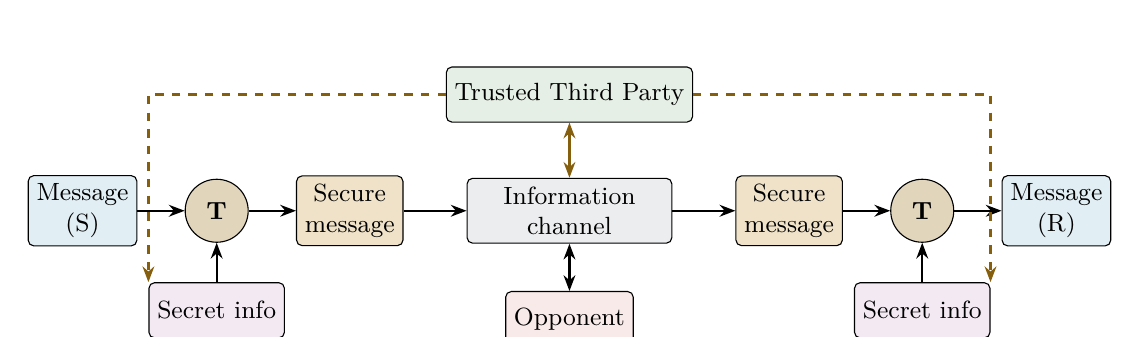
\begin{tikzpicture}[node distance=6mm]
  \node[box,fill=cyan!10] (m1) {Message\\(S)};
  \node[circ,right=of m1] (t1) {T};
  \node[box,below=5mm of t1,fill=magenta!8] (k1) {Secret info};
  \node[box,right=of t1,fill=yellow!20] (c1) {Secure\\message};
  \node[box,right=8mm of c1,minimum width=26mm,fill=gray!15] (ch) {Information\\channel};
  \node[box,right=8mm of ch,fill=yellow!20] (c2) {Secure\\message};
  \node[circ,right=of c2] (t2) {T};
  \node[box,below=5mm of t2,fill=magenta!8] (k2) {Secret info};
  \node[box,right=of t2,fill=cyan!10] (m2) {Message\\(R)};
  \node[box,below=6mm of ch,fill=red!10] (op) {Opponent};
  \node[box,above=7mm of ch,fill=green!12] (ttp) {Trusted Third Party};
  \draw[arr] (m1)--(t1); \draw[arr] (k1)--(t1); \draw[arr] (t1)--(c1);
  \draw[arr] (c1)--(ch); \draw[arr] (ch)--(c2);
  \draw[arr] (c2)--(t2); \draw[arr] (k2)--(t2); \draw[arr] (t2)--(m2);
  \draw[darr] (op)--(ch);
  \draw[darr,orange!80!black] (ttp)--(ch);
  \draw[arr,orange!80!black,dashed] (ttp.west) -| (k1.north west);
  \draw[arr,orange!80!black,dashed] (ttp.east) -| (k2.north east);
\end{tikzpicture}
\end{center}

\textbf{The transformation and the secret.} Instead of sending the plaintext message, $S$ passes it through a \textbf{security-related transformation} $T$. The transformation has two inputs: the message and a piece of \textbf{secret information} (normally a \textbf{key}, a string of bits that selects one particular transformation out of a whole family). Its output is the \textbf{secure message}, for example a ciphertext. At the other end $R$ applies the complementary transformation with its own copy of the secret information and gets the original message back. Stallings sums up the model in one sentence: \imp{every technique for providing security has two components, a security-related transformation of the information to be sent and some secret information shared by the two principals.}

\textbf{Why $T$ and not $E$.} The box is labelled $T$ rather than $E$ (encryption) because encryption is only one kind of transformation. \textbf{Steganography}, which hides the message inside an innocent-looking carrier such as an image or an audio file so that its very existence is concealed, is another; appending an authentication code or a signature to the message is a third. The model covers all of them.

\textbf{What the opponent can do.} The opponent sits on the channel and can intercept the secure message, but since it was transformed with a secret he does not have, he cannot recover the content. Security therefore does \emph{not} come from hiding how $T$ works: the algorithms are public and standardised. It comes from two things: the strength of the algorithm, and the secrecy and length of the key. If the key can take only a few values, the opponent simply tries all of them (a brute-force attack, \S\ref{sec:bruteforce}); every extra key bit doubles his work.

\textbf{The trusted third party.} A \textbf{trusted third party} (TTP) is an entity that both principals trust and that the opponent cannot impersonate. It may be needed to \emph{distribute} the secret information to $S$ and $R$ while keeping it from the opponent (a key distribution centre), to \emph{certify} public keys, or to \emph{arbitrate} disputes between the principals about whether a message was really sent or received. A familiar example is the certificate authority (CA) that signs a bank's SSL/TLS certificate: when a customer opens the bank's website, the browser trusts the bank's public key only because a CA it already trusts vouches for it. The details come in key management (\S\ref{sec:keymgmt}).

\subsection{Four tasks in designing a security service}
Each component of the model turns into one design task. A transformation is needed, so an algorithm must be designed; the algorithm needs secret information, so keys must be generated; both principals need the same (or matching) secret information, so it must be distributed; and the principals must use all of this in the same way, so a protocol must be fixed.

\begin{mustknow}[: the four tasks (Stallings)]
\begin{enumerate}[leftmargin=1.5em]
  \item \textbf{Design an algorithm} for performing the security-related transformation (encryption at $S$, decryption at $R$), such that an opponent cannot defeat its purpose.
  \item \textbf{Generate the secret information} to be used with the algorithm: keys large and random enough that guessing or exhaustive search is infeasible.
  \item \textbf{Develop methods for the distribution and sharing} of the secret information, so that $S$ and $R$ obtain it without the opponent learning it.
  \item \textbf{Specify a protocol} to be used by the two principals that makes use of the algorithm and the secret information to achieve a particular security service (e.g.\ SSL/TLS, IPsec).
\end{enumerate}
Memory aid: \emph{Algorithm $\to$ Key $\to$ Distribute $\to$ Protocol}.
\end{mustknow}

Task 1 is where cryptographic design happens (the ciphers of the coming chapters). Task 2 is harder than it looks, because a key produced by a predictable process (a timestamp, a weak random-number generator) shrinks the effective key space no matter how long the key is. Task 3 is the \emph{key distribution problem}: in symmetric cryptography both principals need the same key, and sending it over the channel it is meant to protect defeats the purpose; it is solved by a TTP, by public-key methods or by Diffie--Hellman. Task 4 exists because a strong algorithm with good keys can still be used insecurely: the protocol fixes the message formats, the order of messages and the checks each party performs, which is what SSL/TLS and IPsec standardise.

\section{Network Access Security Model}\label{sec:accessmodel}

The first model protects a \emph{message in transit}. A second class of threats targets an \emph{information system} itself: an opponent tries to get into a computer system through the network, to read or change the data stored there or to disrupt its service. Stallings divides such threats into \textbf{information access threats}, which intercept or modify data on behalf of users who should not have access to it, and \textbf{service threats}, which exploit flaws in services to stop legitimate users from using them.

\begin{center}
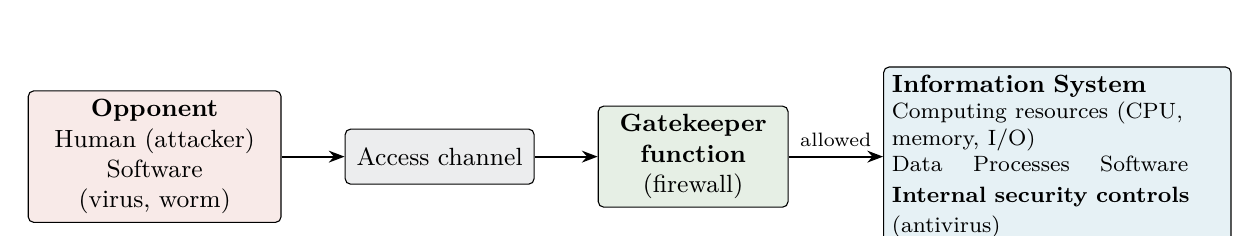
\begin{tikzpicture}[node distance=8mm]
  \node[box,fill=red!10,text width=30mm] (op) {\textbf{Opponent}\\Human (attacker)\\Software (virus, worm)};
  \node[box,right=of op,fill=gray!15,minimum width=24mm] (ac) {Access channel};
  \node[box,right=of ac,fill=green!12,text width=22mm] (gk) {\textbf{Gatekeeper function}\\(firewall)};
  \node[box,right=12mm of gk,fill=cyan!8,text width=42mm,align=left] (is) {\textbf{Information System}\\
    \footnotesize Computing resources (CPU, memory, I/O)\\ \footnotesize Data \quad Processes \quad Software\\
    \footnotesize\textbf{Internal security controls} (antivirus)};
  \draw[arr] (op)--(ac); \draw[arr] (ac)--(gk); \draw[arr] (gk)--node[above,font=\scriptsize]{allowed} (is);
\end{tikzpicture}
\end{center}

The \textbf{opponent} may be a human (a hacker who breaks in for the challenge, a criminal after money, a disgruntled ex-employee) or software (viruses, worms, Trojan horses), which may arrive over the network or on a USB stick. It reaches the system through the \textbf{access channel}, normally the Internet. The \textbf{information system} contains the assets to be protected: computing resources (processor, memory, I/O), data, running processes and installed software.

Defence is placed in two layers. The \textbf{gatekeeper function} is the first line, like a guard at a gate: it examines everything that comes in through the access channel and admits only what is allowed. Firewalls, packet filters, password-based login procedures and screening logic that rejects worms and viruses all belong here. Since no gate is perfect and some attacks start inside, the second line consists of \textbf{internal security controls}, which run inside the system and watch its activity and stored information to detect and contain whatever got past the gate: antivirus software, file-integrity checkers, intrusion detection and operating-system access permissions.

\textbf{Insiders.} An employee who misuses legitimate access never passes the gatekeeper, so only the internal controls can catch him. Insider attacks can do great damage, but the model is drawn mainly for the outside opponent, who must come through the access channel.

\begin{center}\small
\begin{tabularx}{\textwidth}{@{}l X X@{}}
\toprule
 & Model for network security & Network access security model\\
\midrule
Protects & a message while it travels from $S$ to $R$ & an information system and the resources inside it\\
Opponent & on the channel, between the principals & outside the system, trying to get in (or an insider)\\
Defence & security-related transformation with secret information (encryption, MAC, signature) & gatekeeper (firewall, login) plus internal security controls (antivirus, IDS)\\
Extra party & trusted third party for keys and disputes & none required\\
\bottomrule
\end{tabularx}
\end{center}

\section{Cryptography}\label{sec:cryptobasics}

The Concise Oxford English Dictionary defines cryptography as ``the art of writing or solving codes''. The definition used in this course (Stallings, quoted in the lecture) is more precise:
\begin{center}
\imp{Cryptography is the art or science encompassing the principles and methods of transforming an intelligible}\\
\imp{message into one that is unintelligible, and then retransforming that message back to its original form.}
\end{center}
\textbf{Intelligible} means readable by anyone; \textbf{unintelligible} means meaningless to anyone who does not hold the key; \textbf{retransforming} means the process must be reversible by the intended receiver. The word ``art'' reflects that classical ciphers were designed by ingenuity; modern cryptography is a science built on mathematics and complexity theory.

\textbf{Terminology.} The original message is the \textbf{plaintext} (clear text) and the coded message is the \textbf{ciphertext}. Converting plaintext to ciphertext is \textbf{enciphering} or \textbf{encryption}; recovering the plaintext is \textbf{deciphering} or \textbf{decryption}. The scheme used is a \textbf{cryptographic system} or \textbf{cipher}, and the \textbf{key} is the input to the cryptographic algorithm that selects the particular transformation. The slides contrast \textbf{cryptography}, the science of creating coded messages, with \textbf{cryptanalysis}, the art of breaking them, i.e.\ recovering the plaintext or the key without being told the key. The two together form \textbf{cryptology}.

\textbf{Scope today.} Cryptography now covers much more than secret writing: mechanisms for ensuring integrity, techniques for exchanging secret keys, protocols for authenticating users, electronic auctions and elections, and digital cash. Forouzan groups the tools into three mechanisms: \textbf{symmetric-key encipherment}, \textbf{asymmetric-key encipherment} and \textbf{hashing}.

\subsection{Symmetric cipher model}
A symmetric (conventional, single-key) cipher has five ingredients (Stallings): the \textbf{plaintext}; the \textbf{encryption algorithm}, which performs substitutions and transformations on the plaintext; the \textbf{secret key}, also an input to the encryption algorithm, which determines the exact substitutions and transformations; the \textbf{ciphertext}, which depends on both the plaintext and the key, so that two different keys give two different ciphertexts for the same message; and the \textbf{decryption algorithm}, which is the encryption algorithm run in reverse with the same key.

\begin{center}
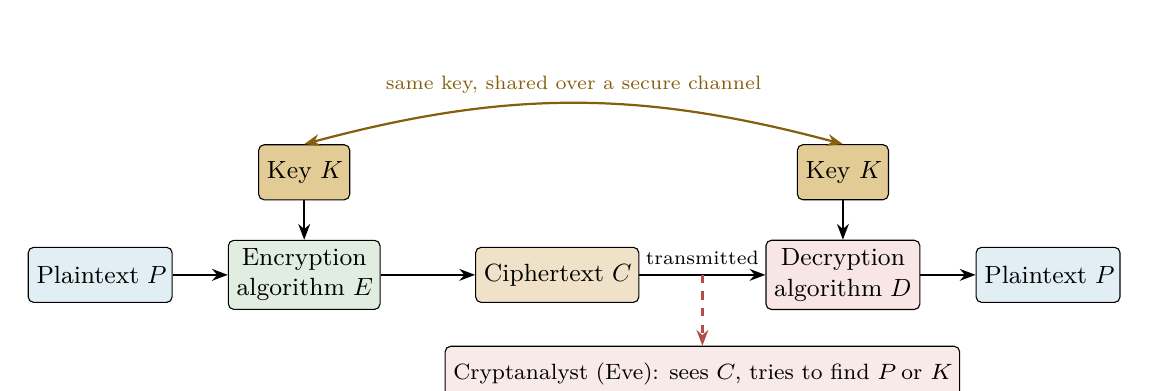
\begin{tikzpicture}[node distance=7mm]
  \node[box,fill=cyan!10] (p1) {Plaintext $P$};
  \node[box,right=of p1,fill=green!15] (e) {Encryption\\algorithm $E$};
  \node[box,right=12mm of e,fill=yellow!20] (c) {Ciphertext $C$};
  \node[box,right=16mm of c,fill=red!12] (d) {Decryption\\algorithm $D$};
  \node[box,right=of d,fill=cyan!10] (p2) {Plaintext $P$};
  \node[box,above=5mm of e,fill=yellow!40] (k1) {Key $K$};
  \node[box,above=5mm of d,fill=yellow!40] (k2) {Key $K$};
  \draw[arr] (p1)--(e); \draw[arr] (k1)--(e); \draw[arr] (e)--(c);
  \draw[arr] (c)--node[above,font=\scriptsize]{transmitted}(d); \draw[arr] (k2)--(d); \draw[arr] (d)--(p2);
  \draw[darr,bend left=15,orange!80!black] (k1.north) to node[above,font=\scriptsize]{same key, shared over a secure channel} (k2.north);
  \coordinate (mid) at ($(c.east)!0.5!(d.west)$);
  \node[box,below=9mm of mid,fill=red!10,font=\footnotesize] (eve) {Cryptanalyst (Eve): sees $C$, tries to find $P$ or $K$};
  \draw[arr,dashed,red!70!black] (mid) -- (eve.north);
\end{tikzpicture}
\end{center}
\[
C = E(K, P) \qquad\qquad P = D(K, C) = D\big(K, E(K,P)\big)
\]
Both algorithms take \textbf{two} inputs: encryption takes $P$ and $K$, decryption takes $C$ and $K$. The equation on the right is the correctness requirement: $D$ with key $K$ must be the inverse of $E$ with key $K$, so that applying one after the other returns the original input.

\textbf{Requirements for secure use.} Stallings states two. First, the encryption algorithm must be strong: an opponent who knows the algorithm and holds many ciphertexts, even together with their plaintexts, must be unable to decrypt other ciphertexts or to find the key. Second, sender and receiver must have obtained their copies of the key in a secure fashion and must keep it secure. The algorithms $E$ and $D$ are \textbf{public}; only $K$ is secret (Kerckhoff's principle, \S\ref{sec:attacks}). This is what makes symmetric encryption practical: since the algorithm need not be hidden, manufacturers can build cheap chips implementing it, and the only thing that must be protected is the key.

\textbf{The key is everything.} If the opponent recovers one plaintext, he has read one message. If he recovers the key, he can read \emph{every} past and future message encrypted under it, which is why cryptanalysts aim at the key. In the lecture's toy example both ends use $K = 100$; such a key would be found instantly. Real symmetric keys are 128 or 256 bits long (2048 bits is the size of an RSA modulus, a different kind of key), so exhaustive search is out of reach (\S\ref{sec:schemes}).

\subsection{Types of cryptography}
Cryptosystems are classified by the number of keys. In \textbf{symmetric-key} (private-key, secret-key, conventional) cryptography one secret key, known only to $S$ and $R$, is used both to encrypt and to decrypt. In \textbf{asymmetric-key} (public-key) cryptography each user has a \textbf{key pair}: one key encrypts and a different but mathematically related key decrypts. One key of the pair is published (the \textbf{public key}) and the other is kept by its owner (the \textbf{private key}). The lecture's toy question, ``can we encrypt with 100 and decrypt with 500?'', has the answer \emph{yes}, provided the two numbers satisfy a mathematical relationship that makes decryption undo encryption, and provided the private key cannot be computed from the public one in practice (RSA, \S\ref{sec:rsa}, is the standard example).
\begin{center}
\small
\begin{tabularx}{\textwidth}{@{}l X X@{}}
\toprule
 & \textbf{Symmetric} (private / secret key) & \textbf{Asymmetric} (public key) \\
\midrule
Keys & One shared key & Key pair: public + private \\
Use & Same key encrypts and decrypts & One key encrypts, the other (mathematically related) decrypts \\
Secrecy & Key known only to $S$ and $R$ & Public key published; private key kept by owner \\
Toy example & Encrypt 100, decrypt 100 & Encrypt 100, decrypt 500 \\
Based on & substitution and permutation of symbols & number theory (factoring, discrete logarithms) \\
Speed and use & fast; bulk data & slow; key exchange, signatures \\
\bottomrule
\end{tabularx}
\end{center}

\textbf{Three dimensions (Stallings).} A cryptographic system is characterised along three independent dimensions. (1) The \textbf{type of operation} used to turn plaintext into ciphertext: \emph{substitution}, in which each element is mapped to another element, and \emph{transposition}, in which elements are rearranged; no information may be lost, so that the operations can be undone, and most real systems, called \emph{product systems}, use several stages of both. (2) The \textbf{number of keys}: one for symmetric, two for asymmetric. (3) The \textbf{way the plaintext is processed}: a \emph{block cipher} processes one block of elements at a time and produces an output block for each input block, while a \emph{stream cipher} processes the input continuously, one element at a time (\S\ref{sec:modern}).

\section{Security of Encryption Schemes}\label{sec:schemes}

Calling a cipher ``secure'' needs a definition: secure against an opponent with how much ciphertext, how much computing power and how much time? Two standards are used.

\textbf{Unconditional security.} \imp{An encryption scheme is unconditionally secure if the ciphertext generated by the scheme does not contain enough information to determine uniquely the corresponding plaintext, no matter how much ciphertext is available.} The guarantee holds against an opponent with unlimited time and computing power, because the obstacle is not the amount of work but the absence of information: every candidate plaintext remains possible and equally likely after the ciphertext is seen. Shannon (1949) called this \textbf{perfect secrecy}.

A one-letter example shows how this is possible. Encrypt a single letter $p$ with a shift cipher, $C = (p + k) \bmod 26$, where the key $k$ is chosen uniformly at random from $0, \dots, 25$ and used only for this letter. For any ciphertext letter $c$ and \emph{any} candidate plaintext $p$ there is exactly one key that maps $p$ to $c$, namely $k = (c - p) \bmod 26$. Each candidate therefore has the same probability $1/26$ of producing the observed $c$, so seeing $c$ tells the opponent nothing about $p$, and trying all 26 keys just lists all 26 letters. Extending this to a long message with a fresh random key for every letter gives the \textbf{one-time pad} (\S\ref{sec:otp}), the only practical unconditionally secure cipher. The price is visible in the argument: the key must be truly random, as long as the message, and never reused, which makes key distribution as hard as sending the message itself.

\textbf{Computational security.} Practical ciphers reuse a short key for long messages, so the ciphertext \emph{does} determine the plaintext in principle; the opponent's problem is only the amount of work. Such a scheme is called computationally secure if it meets either of two criteria:
\begin{mustknow}[: the two definitions]
\textbf{Unconditionally secure}: the ciphertext does not contain enough information to determine the plaintext uniquely, no matter how much ciphertext is available (holds even against unlimited computing power; example: one-time pad).\\[2pt]
\textbf{Computationally secure}: either (1) the \textbf{cost} of breaking the cipher exceeds the \textbf{value} of the encrypted information, or (2) the \textbf{time} required to break the cipher exceeds the \textbf{useful lifetime} of the information.
\end{mustknow}
The cost criterion says that breaking is pointless when it is unprofitable: spending \$1{,}000{,}000 of computing to steal a \$1{,}000 transfer is a loss. The time criterion says that breaking is pointless when it is too late: a price quote valid for 10 minutes that takes 50 years to crack is worthless when cracked. Almost all ciphers in use (AES, RSA) are only computationally secure, since unconditional security needs a key as long as all the data ever sent.

\textbf{Estimating the work: brute force.} The one attack that works against every cipher is \textbf{exhaustive key search}: try every key until the output is meaningful plaintext. If there are $N$ keys and the correct one is equally likely to be any of them, the attacker finds it after $1, 2, \dots, N$ trials with equal probability, so the expected number of trials is $(1 + 2 + \cdots + N)/N = (N+1)/2 \approx N/2$. A $b$-bit key gives $N = 2^b$, so each extra bit doubles the work. The table gives the average search time, computed by script, at $10^9$ decryptions per second (one fast processor) and $10^{13}$ per second (a large parallel machine).
\begin{center}\small
\begin{tabular}{@{}lrrr@{}}
\toprule
Key & Number of keys $N$ & Time at $10^9$/s & Time at $10^{13}$/s\\
\midrule
Shift cipher (Caesar family) & 25 & $1.3 \times 10^{-8}$ s & $1.3 \times 10^{-12}$ s\\
56 bits (DES) & $2^{56} \approx 7.2 \times 10^{16}$ & 1.14 years & 1.0 hour\\
128 bits (AES) & $2^{128} \approx 3.4 \times 10^{38}$ & $5.4 \times 10^{21}$ years & $5.4 \times 10^{17}$ years\\
168 bits (triple DES) & $2^{168} \approx 3.7 \times 10^{50}$ & $5.9 \times 10^{33}$ years & $5.9 \times 10^{29}$ years\\
256 bits (AES) & $2^{256} \approx 1.2 \times 10^{77}$ & $1.8 \times 10^{60}$ years & $1.8 \times 10^{56}$ years\\
26-letter permutation (monoalphabetic) & $26! \approx 4.0 \times 10^{26}$ & $6.4 \times 10^{9}$ years & $6.4 \times 10^{5}$ years\\
\bottomrule
\end{tabular}
\end{center}
The universe is about $1.4 \times 10^{10}$ years old, so a 128-bit key meets the time criterion for any information whatsoever, while a 56-bit key no longer does. Two cautions follow. Brute force also needs the attacker to \emph{recognise} the correct plaintext; this is easy for English text but harder if the plaintext was compressed or is random binary data. And a large key space is necessary but not sufficient: the monoalphabetic cipher has $26!$ keys yet falls in minutes to frequency analysis, which never tries keys at all. Computational security is therefore never proved; a cipher is accepted as computationally secure when the best \emph{known} attack is still too expensive.

\begin{center}\small
\begin{tabularx}{\textwidth}{@{}l X X@{}}
\toprule
 & Unconditionally secure & Computationally secure\\
\midrule
Opponent assumed & unlimited time and computing power & realistic resources and time\\
Why it cannot be broken & ciphertext carries no information about the plaintext & breaking costs more or takes longer than the information is worth\\
Key requirement & random, as long as the message, used once & short key (128--256 bits) reused for many messages\\
Proof & information-theoretic (Shannon) & none; based on the best known attack\\
Example & one-time pad & AES, RSA, DES (in its time)\\
\bottomrule
\end{tabularx}
\end{center}

\begin{trap}[: what ``secure'' does and does not mean]
The Caesar cipher is neither: it is broken in seconds (\S\ref{sec:bruteforce}). Computationally secure does not mean ``unbreakable''; it means ``not worth breaking'' or ``not breakable in time'', and it can be lost when computers get faster (DES) or a better attack is found. Write both criteria of computational security, joined by \emph{either}, and use the words cost/value and time/useful lifetime.
\end{trap}

% College Lecture 3 (security goals, attacks) + Lecture 5 (Kerckhoff, cryptanalysis attack types)
\section{Security Goals, Attacks and Cryptanalysis}\label{sec:attacks}

\subsection{Security goals (CIA)}
\begin{center}\small
\begin{tabularx}{\textwidth}{@{}l X@{}}
\toprule
\textbf{Confidentiality} & hide information from unauthorised access, in storage \emph{and} in transmission (military secrets, bank accounts).\\
\textbf{Integrity} & changes only by authorised entities through authorised mechanisms. Violation need not be malicious (a power surge can corrupt data).\\
\textbf{Availability} & information must be accessible to authorised entities when needed; unavailability is as harmful as a breach.\\
\bottomrule
\end{tabularx}
\end{center}

\subsection{Attacks (Forouzan's taxonomy)}
\begin{center}\small
\begin{tabularx}{\textwidth}{@{}l l l X@{}}
\toprule
Attack & Threatens & Type & What happens\\
\midrule
\textbf{Snooping} & confidentiality & passive & unauthorised access/interception of data. Counter: encipherment.\\
\textbf{Traffic analysis} & confidentiality & passive & learning addresses, timing, request/response pairs from traffic even when it's encrypted.\\
\textbf{Modification} & integrity & active & intercept and change (or delete, delay) a message.\\
\textbf{Masquerading} (spoofing) & integrity & active & impersonating someone (stolen card + PIN; a fake bank site).\\
\textbf{Replaying} & integrity & active & capture a message and resend it later (a second payment).\\
\textbf{Repudiation} & integrity & active & a \emph{party to the communication} denies having sent or received a message.\\
\textbf{Denial of service} & availability & active & slow down or stop the service (bogus requests; deleting responses).\\
\bottomrule
\end{tabularx}
\end{center}
\textbf{Passive} attacks only obtain information: they don't change data, are hard to \emph{detect}, and are prevented by encipherment. \textbf{Active} attacks change data or harm the system: they are easier to detect than to prevent.

\textbf{Stallings' four-way picture} (normal flow source $\to$ destination): \textbf{interruption} (availability), \textbf{interception} (confidentiality), \textbf{modification} (integrity), \textbf{fabrication} (authenticity / masquerade).

\begin{trap}[: repudiation is not an outsider attack]
Every other attack is by a third party (Eve). Repudiation is done by Alice or Bob themselves. It is countered by digital signatures (non-repudiation), not encryption.
\end{trap}

\subsection{Kerckhoff's principle and cryptanalysis attacks \hot}
\asked{2024--25 Q3(a): Eve types ``abcdefghij'' on Alice's computer and reads the output: which attack? (\textbf{chosen-plaintext}, since she chose the plaintext and saw its ciphertext).}
\textbf{Kerckhoff's principle}: assume Eve knows the algorithm; security must rest \emph{only} on the secrecy of the key.
\begin{center}\small
\begin{tabularx}{\textwidth}{@{}l X X@{}}
\toprule
Attack & Eve has & Note\\
\midrule
\textbf{Ciphertext-only} & only ciphertext & most probable. Methods: brute force (key space must be huge), statistical (letter frequencies), pattern attacks.\\
\textbf{Known-plaintext} & earlier plaintext/ciphertext pairs (same key) & easier, less likely (key may have changed).\\
\textbf{Chosen-plaintext} & pairs for plaintexts she chose (access to Alice's machine) & much easier, much less likely.\\
\textbf{Chosen-ciphertext} & plaintexts for ciphertexts she chose (access to Bob's machine) & \\
\bottomrule
\end{tabularx}
\end{center}

\subsection{History notes from the slides}
Atbash (Hebrew, reversed alphabet), scytale (Greek, rod transposition), Caesar (shift 3), Vigen\`ere (1587, broken by Kasiski 1863), Enigma (Scherbius 1918, rotor machine), Shannon (1949, proved OTP unbreakable), DES (IBM, 1970s), Diffie--Hellman (1976), RSA (1977), ECC (Miller, Koblitz 1985), MD5 (Rivest 1991), AES (2001), SHA-512 (2001).

\textbf{ADFGVX} (German army, WWI): a keyed $6 \times 6$ Polybius square (letters $+$ digits, rows/columns labelled A D F G V X) followed by a \textbf{columnar transposition}.
\begin{center}\small
\begin{tabular}{@{}c|cccccc@{}}
 & A&D&F&G&V&X\\ \midrule
A&1&4&7&r&e&g\\
D&i&m&n&t&a&b\\
F&c&d&f&h&j&k\\
G&l&o&p&q&s&u\\
V&v&w&x&y&z&0\\
X&2&3&5&6&8&9\\
\end{tabular}
\quad
\begin{minipage}{0.55\textwidth}
Square keyword \ttx{147regiment} (then the rest of a--z, 0--9). Encrypt \ttx{attackat1200am}: $a \to$ DV, $t \to$ DG, \dots\ giving \ttx{DVDGDGDVFAFXDVDGAAXAVXVXDVDD}. Write it under the transposition key \ttx{PRIVACY}, read columns in alphabetical order of the key letters (A, C, I, P, R, V, Y):\\
\ttx{DXXV GDAD DAAX DVDX VFGV GFAD DVVD} (verified).
\end{minipage}
\end{center}

\begin{fixbox}
\begin{itemize}
  \item Slide 13's figure lists replaying under integrity (correct) but places it visually near confidentiality; use the table above.
  \item The ADFGVX decryption example (keys \ttx{monkeys}/\ttx{zebras}): the transposition step with key \ttx{zebras} does give the slide's intermediate text \ttx{GXFGAXXFDFDAFXDDDXGAAXDFGG}, but a square built from \ttx{monkeys} does not give ``the way is clear''; the slide's square is a different (unshown) one. Learn the method from the encryption example.
\end{itemize}
\end{fixbox}

% Sources: Neso videos (classical techniques, Caesar part 1 & 2: shift cipher, brute force; crypto/notes2.md), slides L1
% (Caesar, monoalphabetic), older L4b/L5 slides (additive cipher, Forouzan Examples 3.3--3.5), Stallings 2.2.
% Every ciphertext and table recomputed by script (scratchpad/r1/verify.py, stat.py).
\section{Classical Encryption Techniques}\label{sec:classical}

Plaintext sent in the open over a public channel invites both kinds of attack (\S\ref{sec:attacks}): \textbf{passive} attacks, in which the opponent eavesdrops and reads the data, and \textbf{active} attacks, in which he alters or injects data. Encryption turns the plaintext into ciphertext so that an interceptor learns nothing from it.

\textbf{Classical} techniques are the ciphers used before computers, operating on the letters of a natural-language alphabet. All of them are now \textbf{obsolete}: they are easy to break and their keys are recovered quickly, often by hand. They are still studied for two reasons. Every modern cipher is built from the same two operations, \emph{substitution} and \emph{transposition}, only applied to bits and repeated over many rounds (\S\ref{sec:modern}); and the ways classical ciphers fail (small key space, preserved letter frequencies, linearity) are exactly the weaknesses that modern designs are built to avoid.

\subsection{Substitution technique}
In a \textbf{substitution} cipher each letter of the plaintext is \textbf{replaced} by another letter, number or symbol, while the \emph{positions} of the letters stay the same. The cipher is a mapping from the plaintext alphabet to the ciphertext alphabet, and this mapping must be one-to-one: if two plaintext letters were sent to the same ciphertext letter, the receiver could not tell which one was meant, and decryption would be ambiguous. Decryption applies the inverse mapping.

\begin{minipage}[t]{0.48\textwidth}
Key (a mapping table):\quad a$\to$M,\; b$\to$X,\; g$\to$A,\; x$\to$Z\\[3pt]
\begin{tabular}{@{}lccc@{}}
Plaintext  & b & a & g \\
           & $\downarrow$ & $\downarrow$ & $\downarrow$ \\
Ciphertext & \textbf{X} & \textbf{M} & \textbf{A}
\end{tabular}
\end{minipage}\hfill
\begin{minipage}[t]{0.48\textwidth}
In the lecture's example the plaintext \ttx{bag} becomes \ttx{XMA}: each letter is looked up in the table and replaced. The mapping table \emph{is} the key. Sender and receiver must share the same table, so this is symmetric encryption.
\end{minipage}
\medskip

If a given plaintext letter is always replaced by the same ciphertext letter, wherever it occurs, the cipher is \textbf{monoalphabetic} (a one-to-one relationship between plaintext and ciphertext symbols). The Caesar cipher and the general monoalphabetic cipher are of this kind. If the same plaintext letter can be replaced by different ciphertext letters at different positions, the cipher is \textbf{polyalphabetic} (one-to-many), like Vigen\`ere and the one-time pad (\S\ref{sec:poly}, \S\ref{sec:otp}); Playfair and Hill, which substitute groups of letters at once, are filed with them by Forouzan. A monoalphabetic substitution only renames the letters, so the ciphertext has the same frequency profile as the plaintext moved onto different symbols, and that is what frequency analysis exploits.

\subsection{Transposition technique}
A \textbf{transposition} cipher does not replace any letter. It applies a \textbf{permutation}, a rearrangement, to the positions of the plaintext letters, so the ciphertext consists of exactly the plaintext letters in a different order. The permutation is the key.

Plaintext \ttx{NESO} $\to$ \ttx{ESON}, \ttx{SONE}, \ttx{ONES}, \ttx{ENOS}, \dots
\quad e.g.\ \ttx{ESON} takes letters in order $(2,3,4,1)$; \ttx{SONE} takes $(3,4,1,2)$.

The number of possible keys for a block of $n$ letters is the number of orderings of $n$ positions: $n$ choices for the first position, $n - 1$ for the second, and so on, giving $n!$. A 4-letter word has only $4! = 24$ arrangements, so short messages are easy to guess. Since $n!$ grows fast ($10! = 3\,628\,800$, $20! \approx 2.4 \times 10^{18}$), transposition is only effective for \textbf{long} plaintexts. Even then it has a built-in weakness: the letter frequencies of the ciphertext are \emph{identical} to those of the plaintext, so a cryptanalyst sees at once that a transposition was used (English frequencies, but no English words) and can rebuild the text by anagramming common pairs such as \ttx{th} and \ttx{he}. Rail fence and row--column transposition (Transposition Ciphers section) and keyed transposition (\S\ref{sec:classextra}) are the standard examples.

\subsection{Substitution vs.\ transposition}
The two techniques attack the structure of the plaintext from opposite sides: substitution hides \emph{which} letters occur, transposition hides \emph{where} they occur. Neither alone hides everything, which is why practical ciphers combine them (ADFGVX in 1918, every round of DES and AES today).
\begin{center}\small
\begin{tabularx}{\textwidth}{@{}l X X@{}}
\toprule
 & \textbf{Substitution} & \textbf{Transposition} \\
\midrule
What changes & The letters themselves & The order of the letters \\
Positions & Unchanged & Permuted \\
Letters in ciphertext & New letters / symbols & Exactly the plaintext letters \\
Letter frequencies & Moved onto different symbols & Identical to plaintext \\
Key & a mapping of the alphabet (e.g.\ a shift) & a permutation of positions \\
Weak against & frequency analysis (monoalphabetic) & anagramming; short messages ($n!$ small) \\
\bottomrule
\end{tabularx}
\end{center}

\begin{center}
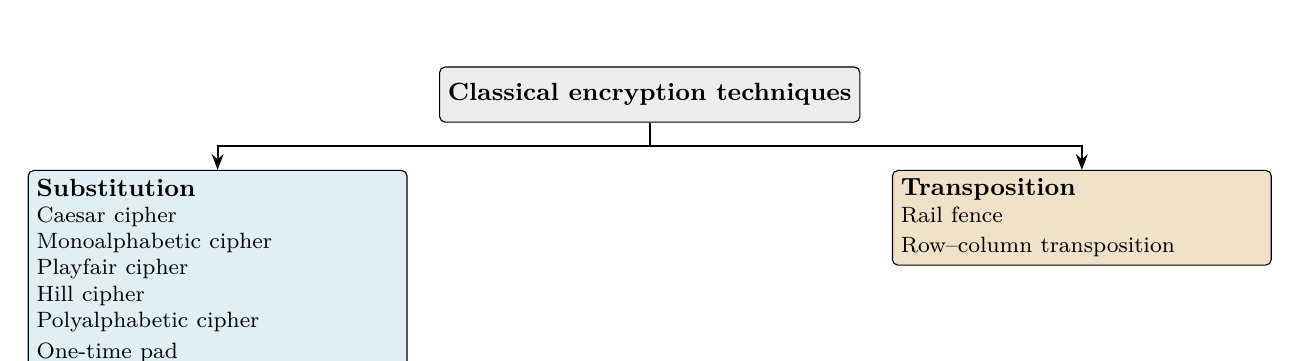
\begin{tikzpicture}[node distance=5mm]
  \node[box,fill=gray!15] (root) {\textbf{Classical encryption techniques}};
  \node[box,fill=cyan!10,below left=6mm and 4mm of root,text width=46mm,align=left] (sub) {\textbf{Substitution}\\
  \footnotesize Caesar cipher\\ \footnotesize Monoalphabetic cipher\\ \footnotesize Playfair cipher\\ \footnotesize Hill cipher\\ \footnotesize Polyalphabetic cipher\\ \footnotesize One-time pad};
  \node[box,fill=yellow!20,below right=6mm and 4mm of root,text width=46mm,align=left] (tra) {\textbf{Transposition}\\
  \footnotesize Rail fence\\ \footnotesize Row--column transposition};
  \draw[arr] (root.south) -- ++(0,-3mm) -| (sub.north);
  \draw[arr] (root.south) -- ++(0,-3mm) -| (tra.north);
\end{tikzpicture}
\end{center}

\section{Caesar Cipher}\label{sec:caesar}

The Caesar cipher is the earliest known and simplest substitution cipher, used by Julius Caesar for military messages. \imp{Each letter of the alphabet is replaced by the letter standing three places further down the alphabet,} and the alphabet is treated as a circle, so that after \ttx{z} it wraps round to \ttx{a}:
\begin{center}\small\ttfamily\setlength{\tabcolsep}{3.2pt}
\begin{tabular}{@{}l*{26}{c}@{}}
\rmfamily plain: & a&b&c&d&e&f&g&h&i&j&k&l&m&n&o&p&q&r&s&t&u&v&w&x&y&z\\
\rmfamily cipher: & D&E&F&G&H&I&J&K&L&M&N&O&P&Q&R&S&T&U&V&W&X&Y&Z&A&B&C\\
\end{tabular}
\end{center}
Since every letter is moved by the same amount and a letter is always replaced by the same letter, it is a monoalphabetic substitution. Stallings' classic example: \ttx{meet me after the toga party} $\to$ \ttx{PHHW PH DIWHU WKH WRJD SDUWB}.

\subsection{Letters as numbers (start at 0)}
To write the rule as a formula, each letter is replaced by its position in the alphabet, starting from 0:
\begin{center}\small\setlength{\tabcolsep}{4pt}
\begin{tabular}{*{13}{c}}
\toprule
A&B&C&D&E&F&G&H&I&J&K&L&M\\
0&1&2&3&4&5&6&7&8&9&10&11&12\\
\midrule
N&O&P&Q&R&S&T&U&V&W&X&Y&Z\\
13&14&15&16&17&18&19&20&21&22&23&24&25\\
\bottomrule
\end{tabular}
\end{center}
Numbering from 0 matches the remainders mod 26, which are exactly $0,1,\dots,25$. The wrap-around from \ttx{z} to \ttx{a} is then simply reduction modulo 26, i.e.\ arithmetic in $\mathbb{Z}_{26}$ (\S\ref{sec:modular}). If the letters were numbered 1 to 26, \ttx{z} would be 26, which reduces to 0, a number that stands for no letter.

\subsection{Algorithm}
With $p$ the number of a plaintext letter, $C$ the number of the ciphertext letter and $k$ the key (the shift), encryption adds the key and decryption subtracts it, both modulo 26.
\begin{mustknow}[: Caesar / shift cipher]
\vspace{-6pt}
\begin{align*}
C &= E(p,k) = (p + k) \bmod 26\\
p &= D(C,k) = (C - k) \bmod 26
\end{align*}
Caesar cipher: $k = 3$. Shift cipher: any $k \in \{1, \dots, 25\}$.
\end{mustknow}

\begin{minipage}[c]{0.55\textwidth}
\textbf{Why decryption works.} Decrypting the encryption gives $\big((p + k) \bmod 26 - k\big) \bmod 26 = p \bmod 26$, because reducing modulo 26 before or after the subtraction gives the same remainder. Since $0 \le p \le 25$, this is exactly $p$.

\textbf{Computing the remainder.} \textbf{mod gives the remainder, not the quotient}: $27 \bmod 26 = 1$, because $27 = 1 \times 26 + 1$. During decryption $C - k$ can be negative; the remainder must lie in $0, \dots, 25$, so add 26: $-2 \bmod 26 = 24$, because $-2 = (-1) \times 26 + 24$.

\textbf{Convention.} Plaintext is written in lowercase and ciphertext in UPPERCASE, which keeps the two apart in a worked answer. For letters away from the end of the alphabet one can simply count $k$ letters forward; the formula matters at the wrap-around.
\end{minipage}\hfill
\begin{minipage}[c]{0.42\textwidth}
\centering
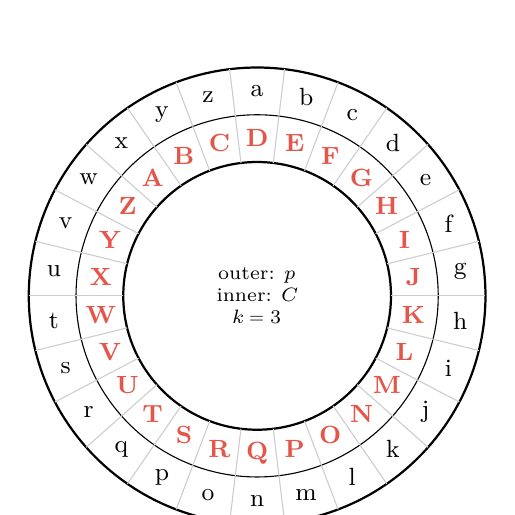
\begin{tikzpicture}
  \draw[thick] (0,0) circle (2.9);
  \draw (0,0) circle (2.3);
  \draw[thick] (0,0) circle (1.7);
  \foreach \pl/\cl [count=\n from 0] in {a/D,b/E,c/F,d/G,e/H,f/I,g/J,h/K,i/L,j/M,k/N,l/O,m/P,n/Q,o/R,p/S,q/T,r/U,s/V,t/W,u/X,v/Y,w/Z,x/A,y/B,z/C}{
    \pgfmathsetmacro{\ang}{90-\n*360/26}
    \pgfmathsetmacro{\sep}{\ang+180/26}
    \node[font=\small] at (\ang:2.6) {\pl};
    \node[font=\small\bfseries,text=warn] at (\ang:2.0) {\cl};
    \draw[gray!50] (\sep:1.7) -- (\sep:2.9);
  }
  \node[font=\scriptsize,align=center] at (0,0) {outer: $p$\\inner: $C$\\$k=3$};
\end{tikzpicture}
\end{minipage}

\subsection{Worked example: encrypt ``neso academy'' ($k=3$)}
\begin{worked}[: Caesar encryption (lecture example)]
\textbf{Q.} Encrypt ``neso academy'' using the Caesar cipher.

\textbf{A.} Convert each letter to its number, add 3, reduce mod 26, convert back:
\begin{center}\small\setlength{\tabcolsep}{5pt}
\begin{tabular}{@{}l*{4}{c}|*{7}{c}@{}}
\toprule
Plaintext & n&e&s&o & a&c&a&d&e&m&y\\
$p$ & 13&4&18&14 & 0&2&0&3&4&12&24\\
$p+3$ & 16&7&21&17 & 3&5&3&6&7&15&\hl{27}\\
$\bmod 26$ & 16&7&21&17 & 3&5&3&6&7&15&\hl{1}\\
Ciphertext & \textbf{Q}&\textbf{H}&\textbf{V}&\textbf{R} & \textbf{D}&\textbf{F}&\textbf{D}&\textbf{G}&\textbf{H}&\textbf{P}&\textbf{B}\\
\bottomrule
\end{tabular}
\end{center}
Answer: \textbf{\ttx{QHVR DFDGHPB}}.
The only wrap-around is \ttx{y}: $24+3 = 27$, and $27 = 26\times 1 + \mathbf{1}$, so $C = 1 = $ \ttx{B}.
(Counting on: y $\to$ z $\to$ a $\to$ \textbf{b}.) For the other letters you can just count three letters forward.
\textbf{Check:} $B = 1$, $1 - 3 = -2 \equiv 24 = $ \ttx{y} \checkmark.
\end{worked}

\subsection{Homework 1: decrypt ``QHWZRUN VHFXULWB'' ($k=3$)}
\begin{worked}[: Caesar decryption (lecture homework)]
\textbf{Q.} Decrypt ``QHWZRUN VHFXULWB'' using the Caesar cipher.

\textbf{A.} Apply $p = (C - 3) \bmod 26$ to every letter:
\begin{center}\small\setlength{\tabcolsep}{3.6pt}
\begin{tabular}{@{}l*{7}{c}|*{8}{c}@{}}
\toprule
Ciphertext & Q&H&W&Z&R&U&N & V&H&F&X&U&L&W&B\\
$C$ & 16&7&22&25&17&20&13 & 21&7&5&23&20&11&22&1\\
$C-3$ & 13&4&19&22&14&17&10 & 18&4&2&20&17&8&19&\hl{$-2$}\\
$\bmod 26$ & 13&4&19&22&14&17&10 & 18&4&2&20&17&8&19&\hl{24}\\
Plaintext & n&e&t&w&o&r&k & s&e&c&u&r&i&t&y\\
\bottomrule
\end{tabular}
\end{center}
Answer: \textbf{network security}. Note the last letter: $1-3=-2$, add 26 $\Rightarrow 24 =$ \ttx{y}.
\end{worked}

\section{Shift Cipher (the general form)}\label{sec:shift}

The Caesar cipher has no real key: the shift is always 3, so anyone who knows the method can read every message. The obvious repair is to let the shift vary and keep it secret. The \textbf{shift cipher} uses the same two formulas with a secret key $k$; Forouzan calls it the \textbf{additive cipher}, because encryption is addition in $\mathbb{Z}_{26}$. \textbf{Caesar cipher = shift cipher with $k=3$.}

\textbf{How many keys?} A key $k$ and the key $k + 26$ give the same cipher, since $(p + k + 26) \bmod 26 = (p + k) \bmod 26$; so every key can be reduced modulo 26 (a shift of 29 is a Caesar shift of 3), and there are only 26 different keys, $0$ to $25$. One of them is useless:
\begin{itemize}
  \item $k=0$ is useless: $C = (p+0) \bmod 26 = p$, so the ciphertext equals the plaintext. (Homework: ``Neso'', $k=0$ $\Rightarrow$ \ttx{NESO}.)
  \item $k=26$ is the same as $k=0$. So there are only \textbf{25 usable keys}.
\end{itemize}

\textbf{Decryption is encryption with $26 - k$.} Subtracting $k$ modulo 26 is the same as adding its additive inverse $26 - k$: $(C - k) \bmod 26 = (C + 26 - k) \bmod 26$. Decrypting the Caesar cipher is therefore the same as encrypting with key 23, and an attacker who tries all forward shifts tries all decryption keys too. This is why the forward and backward shifts in the brute-force table below always add up to 26.

\textbf{Encrypting twice does not help.} Shifting by $k_1$ and then by $k_2$ gives $(p + k_1 + k_2) \bmod 26$, which is a single shift by $(k_1 + k_2) \bmod 26$. Double encryption with two shift keys is just another shift cipher, still with 25 keys to search. (In algebraic terms, the shift ciphers are closed under composition.)

\textbf{Example:} ``Neso'', $k=4$: \;
N $13{+}4{=}17\to$\textbf{R},\;
e $4{+}4{=}8\to$\textbf{I},\;
s $18{+}4{=}22\to$\textbf{W},\;
o $14{+}4{=}18\to$\textbf{S} \;$\Rightarrow$\; \textbf{\ttx{RIWS}}.

\textbf{Homework 2:} ``cryptography'', $k=4$:
\begin{center}\small\setlength{\tabcolsep}{4.5pt}
\begin{tabular}{@{}l*{12}{c}@{}}
\toprule
Plaintext & c&r&y&p&t&o&g&r&a&p&h&y\\
$p$ & 2&17&24&15&19&14&6&17&0&15&7&24\\
$p+4 \bmod 26$ & 6&21&\hl{2}&19&23&18&10&21&4&19&11&\hl{2}\\
Ciphertext & G&V&C&T&X&S&K&V&E&T&L&C\\
\bottomrule
\end{tabular}
\end{center}
Answer: \textbf{\ttx{GVCTXSKVETLC}} (both \ttx{y}'s wrap: $24+4=28 \equiv 2$).

\textbf{In code:} the 0--25 numbering is a convention. With ASCII (\ttx{A}=65, \ttx{a}=97), shift to 0 first, then back:
\;$C = \big((p - 65 + k) \bmod 26\big) + 65$ for uppercase (use 97 for lowercase).

\begin{worked}[: Forouzan Example 3.3 (additive cipher)]
\textbf{Q.} Use the additive cipher with key $= 15$ to encrypt the message ``hello''. Decrypt the result to verify.

\textbf{Encryption}, $C = (p + 15) \bmod 26$:
\begin{center}\small\setlength{\tabcolsep}{6pt}
\begin{tabular}{@{}l*{5}{c}@{}}
\toprule
Plaintext & h&e&l&l&o\\
$p$ & 7&4&11&11&14\\
$p + 15$ & 22&19&\hl{26}&\hl{26}&\hl{29}\\
$\bmod 26$ & 22&19&0&0&3\\
Ciphertext & \textbf{W}&\textbf{T}&\textbf{A}&\textbf{A}&\textbf{D}\\
\bottomrule
\end{tabular}
\qquad
\begin{tabular}{@{}l*{5}{c}@{}}
\toprule
Ciphertext & W&T&A&A&D\\
$C$ & 22&19&0&0&3\\
$C - 15$ & 7&4&\hl{$-15$}&\hl{$-15$}&\hl{$-12$}\\
$\bmod 26$ & 7&4&11&11&14\\
Plaintext & h&e&l&l&o\\
\bottomrule
\end{tabular}
\end{center}
Ciphertext \textbf{\ttx{WTAAD}}; decryption with $p = (C - 15) \bmod 26$ (adding 26 to the negative values) returns \textbf{hello} \checkmark. Note that the double \ttx{l} gives the double \ttx{A}: a monoalphabetic cipher keeps repeated letters visible.
\end{worked}

\subsection{Pros and cons of the Caesar cipher}
\textbf{Advantages.} The cipher is \textbf{simple} and \textbf{easy to implement}: it needs one addition per letter and can be done by hand or written in a few lines of code.

\textbf{Disadvantages.} The lecture lists three, and together they are exactly what makes a brute-force attack succeed.
\begin{enumerate}[leftmargin=1.5em]
  \item \textbf{The encryption and decryption algorithms are known.} By itself this is normal (Kerckhoff's principle, \S\ref{sec:attacks}); it means the attacker knows the cipher is a shift and only has to find $k$.
  \item \textbf{There are only 25 keys to try}, so the cipher is vulnerable to a \textbf{brute-force attack}: trying all of them takes seconds.
  \item \textbf{The language of the plaintext is known and easily recognisable}, so the attacker can tell when he has hit the right key, because exactly one trial produces readable text.
\end{enumerate}
A fourth weakness follows from being monoalphabetic with a single shift: letter frequencies survive, so even without trying keys, one correct guess of a single plaintext--ciphertext letter pair reveals the key (statistical attack below).

\section{Brute-Force Attack on the Caesar/Shift Cipher}\label{sec:bruteforce}

A \textbf{brute-force} (exhaustive key search) attack tries every possible key until readable plaintext appears. For the shift cipher this is trivial. There are 25 keys and the right one is equally likely to be any of them, so on average the attacker needs $(1 + 2 + \cdots + 25)/25 = 13$ trials and at worst 25. By hand that is a few minutes of counting; a computer doing $10^9$ trials per second needs about $10^{-8}$ seconds. Compare $2^{128} \approx 3.4 \times 10^{38}$ keys for AES (\S\ref{sec:schemes}): the attack is the same, only the size of the key space differs.

\begin{mustknow}[: when brute force works (Stallings)]
Three conditions make brute-force cryptanalysis of the Caesar cipher easy: (1) the encryption and decryption algorithms are known; (2) there are only 25 keys to try; (3) the language of the plaintext is known and easily recognisable. A cipher defeats brute force by making (2) false: a key space of $2^{128}$ or more.
\end{mustknow}

\textbf{The lecture example.} Ciphertext: \ttx{SQDYMZK}. Shift every letter forward by 0, 1, 2, \dots, 25 and look for a real word:

\begin{center}\small\ttfamily\setlength{\tabcolsep}{6pt}
\begin{tabular}{@{}ccl@{}}
\toprule
\rmfamily\bfseries Fwd & \rmfamily\bfseries Back & \rmfamily\bfseries Result\\
\midrule
0 & 26 & SQDYMZK\\
1 & 25 & TREZNAL\\
2 & 24 & USFAOBM\\
3 & 23 & VTGBPCN\\
4 & 22 & WUHCQDO\\
5 & 21 & XVIDREP\\
6 & 20 & YWJESFQ\\
7 & 19 & ZXKFTGR\\
8 & 18 & AYLGUHS\\
9 & 17 & BZMHVIT\\
10 & 16 & CANIWJU\\
11 & 15 & DBOJXKV$^\ast$\\
12 & 14 & ECPKYLW\\
\bottomrule
\end{tabular}
\qquad
\begin{tabular}{@{}ccl@{}}
\toprule
\rmfamily\bfseries Fwd & \rmfamily\bfseries Back & \rmfamily\bfseries Result\\
\midrule
13 & 13 & FDQLZMX\\
\rowcolor{warn!18} \textbf{14} & \textbf{12} & \textbf{GERMANY}\\
15 & 11 & HFSNBOZ\\
16 & 10 & IGTOCPA\\
17 & 9 & JHUPDQB\\
18 & 8 & KIVQERC\\
19 & 7 & LJWRFSD\\
20 & 6 & MKXSGTE\\
21 & 5 & NLYTHUF\\
22 & 4 & OMZUIVG$^\ast$\\
23 & 3 & PNAVJWH\\
24 & 2 & QOBWKXI\\
25 & 1 & RPCXLYJ\\
\bottomrule
\end{tabular}
\end{center}
{\footnotesize $^\ast$ Recomputed; the notes had these rows slightly wrong (see corrections box).}

Forward $+$ back $= 26$ in every row, because shifting forward 14 is the same as shifting back 12: $\;C + 14 \equiv C - 12 \pmod{26}$ (\S\ref{sec:shift}). Only one row is English, \textbf{GERMANY}, so the attacker now has the plaintext \emph{and} the key.

\textbf{Which number is the key?} The sender encrypted with $k = \mathbf{12}$ (G $6+12=18=$ S, \dots, Y $24+12=36\equiv10=$ K). The 14 is the forward shift that \emph{undoes} it. The lecture calls 14 ``the key''; be clear which one you mean in an exam: write ``encryption key $k = 12$; decryption is a forward shift of 14 (a backward shift of 12)''.

\textbf{Decryption versus cryptanalysis.} \imp{Decryption is done by the receiver, who has the key and reverses the encryption; cryptanalysis is done by an attacker who does not have the key and recovers the plaintext and/or the key}, here by brute force. The table above is cryptanalysis, not decryption.

\textbf{A caution.} Brute force assumes that exactly one trial gives meaningful text. For a long ciphertext this is practically certain, but a very short ciphertext (three or four letters) may decrypt to two different words under two keys, and then the attacker cannot decide without more ciphertext or context.

\begin{worked}[: Forouzan Example 3.4 (brute force)]
\textbf{Q.} Eve has intercepted the ciphertext \ttx{UVACLYFZLJBYL}. Show how she can use a brute-force attack to break the cipher.

\textbf{A.} Eve knows the cipher is additive and that the key domain is $\{1, \dots, 25\}$. She decrypts with $p = (C - k) \bmod 26$ for $k = 1, 2, 3, \dots$ and stops at the first meaningful text:
\begin{center}\small\setlength{\tabcolsep}{8pt}
\begin{tabular}{@{}cl|cl@{}}
\toprule
Key & Plaintext & Key & Plaintext\\
\midrule
1 & \ttx{tuzbkxeykiaxk} & 5 & \ttx{pqvxgtaugewtg}\\
2 & \ttx{styajwdxjhzwj} & 6 & \ttx{opuwfsztfdvsf}\\
3 & \ttx{rsxzivcwigyvi} & \cellcolor{warn!18}\textbf{7} & \cellcolor{warn!18}\textbf{\ttx{notverysecure}}\\
4 & \ttx{qrwyhubvhfxuh} & & \\
\bottomrule
\end{tabular}
\end{center}
The plaintext is \textbf{``not very secure''} and the key is $\mathbf{k = 7}$. \textbf{Check:} \ttx{n} $= 13$, $13 + 7 = 20 = $ \ttx{U}, the first ciphertext letter \checkmark. (The remaining keys 8--25 were also tried by script; none gives English.)
\end{worked}

\textbf{Statistical attack.} The shift cipher also falls without trying keys. Since every letter is shifted by the same $k$, a single correct pair is enough: if ciphertext letter $c$ stands for plaintext letter $p$, then $k = (c - p) \bmod 26$. The attacker counts the ciphertext letters and assumes the most frequent one stands for \ttx{e}, the most common letter in English (about 12.5\% of letters on the slide's chart; then \ttx{t}, \ttx{a}, \ttx{o}). If the result is not readable, the next most frequent letter is tried as \ttx{e}, or the top letter as \ttx{t}. The attack needs a reasonably long ciphertext, because the frequencies of a short text can differ from the averages.

\begin{worked}[: Forouzan Example 3.5 (statistical attack)]
\textbf{Q.} Eve has intercepted the following ciphertext. Using a statistical attack, find the plaintext.\\
\ttx{XLILSYWIMWRSAJSVWEPIJSVJSYVQMPPMSRHSPPEVWMXMWASVX}\\
\ttx{LQSVILYVVCFIJSVIXLIWIPPIVVIGIMZIWQSVISJJIVW}

\textbf{A.} Count the 92 ciphertext letters. The most frequent are \ttx{I} (14 times), \ttx{V} (13) and \ttx{S} (12). Assume \ttx{I} $\to$ \ttx{e}: $k = (8 - 4) \bmod 26 = \mathbf{4}$. Decrypt with $p = (C - 4) \bmod 26$:
\begin{center}\small
\emph{the house is now for sale for four million dollars it is worth more hurry before the seller receives more offers}
\end{center}
The text is English, so the key is $\mathbf{4}$. \textbf{Check:} \ttx{t} $= 19$, $19 + 4 = 23 = $ \ttx{X} \checkmark. (Taking \ttx{V} as \ttx{e} would give $k = 17$ and gibberish; \ttx{V} actually stands for \ttx{r}, which is unusually common in this text.)
\end{worked}

\begin{trap}[: the usual slips with shift ciphers]
The key space is 25, not 26, since $k = 0$ changes nothing. Show the wrap-around step ($27 \bmod 26 = 1$) and turn a negative value into a remainder by adding 26. In a brute-force answer, draw the table, box the readable row and state the \emph{encryption} key (12 in the \ttx{SQDYMZK} example, not 14). Know the three cons of the Caesar cipher, and do not call ``the algorithm is public'' a violation of Kerckhoff's principle: it is what the principle assumes.
\end{trap}

\begin{fixbox}
\begin{itemize}
  \item ``neso academy'' encrypts to \ttx{QHVR DFDGHPB}. The notes' final answer \ttx{QHVRDFDGHB} drops the \ttx{P}.
  \item Brute-force table: row 11 is \ttx{DBOJXKV} and row 22 is \ttx{OMZUIVG}. Row 12 (\ttx{ECPKYLW}) was already correct.
  \item The notes call con \#1 a ``Kerckhoffs violation''. It isn't: public algorithms are normal (see the intro sheet). The problem is a public algorithm \emph{plus} only 25 keys.
  \item Slide typo: ``used \emph{be} Julius Caesar'' $\to$ ``used \emph{by}''.
  \item Shift-cipher slide: ``Key = 2, 3, 4, 5, \dots'' leaves out $k = 1$, which is a valid key; the usable keys are $1, \dots, 25$.
\end{itemize}
\end{fixbox}

% Sources: Neso videos (monoalphabetic; Playfair parts 1-2; Playfair solved question; crypto/notes3.md), college Lecture 5
% (Forouzan 3.2: monoalphabetic key table, statistical attack, Playfair secret key and "hello", cryptanalysis of Playfair),
% Stallings 2.2 (frequency analysis, homophones, Playfair strength). Every number recomputed by script (scratchpad/r2/verify.py).
\providecommand{\NESOACADEMY}{{N,E,S,O,A},{C,D,M,Y,B},{F,G,H,{I/J},K},{L,P,Q,R,T},{U,V,W,X,Z}}
\providecommand{\JUPITER}{{{I/J},U,P,T,E},{R,A,B,C,D},{F,G,H,K,L},{M,N,O,Q,S},{V,W,X,Y,Z}}
\providecommand{\NESOAPP}{{N,E,S,O,A},{P,B,C,D,F},{G,H,{I/J},K,L},{M,Q,R,T,U},{V,W,X,Y,Z}}
\providecommand{\PFFOROUZAN}{{L,G,D,B,A},{Q,M,H,E,C},{U,R,N,{I/J},F},{X,V,S,O,K},{Z,Y,W,T,P}}

\section{Monoalphabetic Cipher}\label{sec:monoalpha}

The Caesar (shift) cipher has two weaknesses that make it useless. Its key space has only 25 useful keys, so an attacker simply tries them all. Worse, every letter is shifted by the \emph{same} amount, so the shift found for a single letter decrypts the whole message. The monoalphabetic cipher removes both weaknesses at once: instead of shifting the alphabet, it replaces each letter by an \emph{arbitrary} other letter, chosen independently for each of the 26 letters. The only constraint is that the replacement must be one-to-one, so that the receiver can undo it.

\subsection{Permutations}
A \imp{permutation of a finite set $S$ is an ordered sequence of all the elements of $S$, with each element appearing exactly once.} The set $S = \{a, b, c\}$ has six permutations: \ttx{abc, acb, bac, bca, cab, cba}. In general a set of $n$ elements has $n! = n(n-1)\cdots 2 \cdot 1$ permutations, because the first position can be filled in $n$ ways, the second in $n - 1$ ways (one element is used up), and so on down to one way for the last position. For example $2! = 2$ and $4! = 24$.

Permutations matter here because the key of a monoalphabetic cipher \emph{is} a permutation of the alphabet: writing the ciphertext letters for $a, b, \dots, z$ in order gives a sequence in which each of the 26 letters appears exactly once. The number of possible keys is therefore the number of permutations of 26 letters, $26!$.

\subsection{The cipher}
In a \textbf{monoalphabetic substitution cipher} Alice and Bob agree on a table that pairs every plaintext letter with one ciphertext letter. The bottom row of the table, the \textbf{cipher line}, can be any permutation of the 26 letters. To encrypt, each plaintext letter is looked up in the top row and replaced by the letter below it; to decrypt, each ciphertext letter is found in the bottom row and replaced by the letter above it. The relationship between plaintext and ciphertext symbols is \textbf{one-to-one}: a plaintext letter always becomes the same ciphertext letter, and no two plaintext letters share a ciphertext letter. If two letters shared one, the receiver could not tell which was meant, so the table would not be decryptable.

The key space has $26! \approx 4.03 \times 10^{26} \approx 2^{88}$ keys, compared with 25 for the shift cipher. A computer testing $10^{12}$ keys per second would need about 13 million years to try them all, so the slide's conclusion is that the large key space ``would seem to eliminate brute-force techniques''. The shift ciphers are just 26 of these $26!$ permutations, those in which the cipher line is the alphabet rotated. Although a permutation is involved, the monoalphabetic cipher is still a \textbf{substitution} cipher: the permutation is applied to the \emph{alphabet} to build the key, while the letters of the message keep their positions. Rearranging the message itself would be a transposition.

\textbf{Example (lecture).} Under one key, ``Neso'' becomes \ttx{DULA}. The distance each letter moves is different, so learning one pair of the table says nothing about the others; with Caesar the distance is always 3.
\begin{center}\small\setlength{\tabcolsep}{6pt}
\begin{tabular}{@{}lcccc@{}}
\toprule
Plaintext & N (13) & E (4) & S (18) & O (14)\\
Ciphertext & \textbf{D} (3) & \textbf{U} (20) & \textbf{L} (11) & \textbf{A} (0)\\
Shift $(C-p) \bmod 26$ & 16 & 16 & 19 & 12\\
\bottomrule
\end{tabular}
\end{center}

\begin{worked}[: the slide's key table (Forouzan)]
\textbf{Q.} Using the key below, encrypt ``this message is easy to encrypt but hard to find the key'', and show how Bob decrypts.
\begin{center}\small\setlength{\tabcolsep}{2.4pt}
\begin{tabular}{@{}l*{26}{c}@{}}
\toprule
Plain & a&b&c&d&e&f&g&h&i&j&k&l&m&n&o&p&q&r&s&t&u&v&w&x&y&z\\
Cipher & N&O&A&T&R&B&E&C&F&U&X&D&Q&G&Y&L&K&H&V&I&J&M&P&Z&S&W\\
\bottomrule
\end{tabular}
\end{center}
\textbf{A.} Remove the spaces and replace each letter by the one below it: t$\to$I, h$\to$C, i$\to$F, s$\to$V, so ``this'' $\to$ \ttx{ICFV}; ``message'' $\to$ \ttx{QRVVNER}; and so on. The ciphertext is
\begin{center}\small\ttfamily ICFVQRVVNERFVRNVSIYRGAHSLIOJICNHTIYBFGTICRXRS\end{center}
Bob finds each ciphertext letter in the bottom row and reads the letter above it (I$\to$t, C$\to$h, F$\to$i, V$\to$s, \dots), which recovers the plaintext. Note that the three \ttx{s} of ``message is'' all became \ttx{V} and every \ttx{e} became \ttx{R}: the frequency pattern of the plaintext survives, which is the subject of the next subsection.
\end{worked}

\subsection{Breaking it: frequency analysis}
The huge key space does not protect the cipher, because the attacker never searches through keys. A monoalphabetic cipher only \emph{renames} letters. If the key maps $x$ to $\pi(x)$, then every occurrence of $x$ in the plaintext becomes an occurrence of $\pi(x)$ in the ciphertext and nothing else becomes $\pi(x)$, so $\pi(x)$ occurs in the ciphertext exactly as often as $x$ occurs in the plaintext. The histogram of ciphertext letters is the histogram of plaintext letters with the bars relabelled. \imp{A monoalphabetic cipher does not change the frequency of characters}, so each letter of the key can be found separately by matching frequencies, and the attack needs a few dozen decisions instead of $26!$ guesses. This is a \textbf{statistical} (frequency) attack, and it needs only the ciphertext, which makes it a ciphertext-only attack, the most likely kind in practice.

The attack works because English letters are far from equally common. The relative frequencies (lecture chart, from a large corpus) are:
\begin{center}
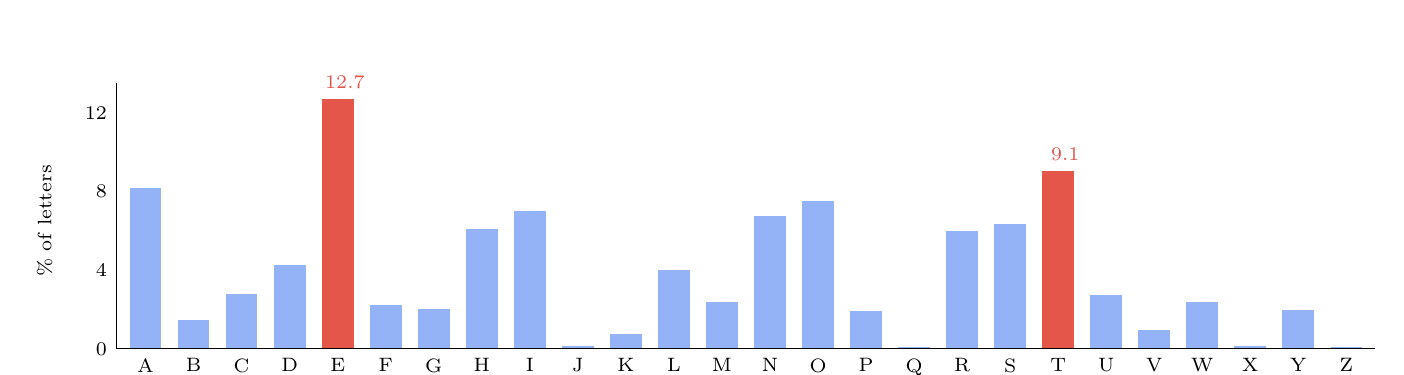
\begin{tikzpicture}[x=6.1mm,y=2.5mm]
  \foreach \L/\v [count=\i] in {A/8.167,B/1.492,C/2.782,D/4.253,E/12.702,F/2.228,G/2.015,H/6.094,I/6.996,J/0.153,K/0.772,L/4.025,M/2.406,N/6.749,O/7.507,P/1.929,Q/0.095,R/5.987,S/6.327,T/9.056,U/2.758,V/0.978,W/2.360,X/0.150,Y/1.974,Z/0.074}{
    \fill[acc!55] (\i-0.33,0) rectangle (\i+0.33,\v);
    \node[font=\scriptsize,below] at (\i,0) {\L};
  }
  \fill[warn] (5-0.33,0) rectangle (5.33,12.702) node[above,font=\scriptsize,xshift=-1.1mm] {12.7};
  \fill[warn] (20-0.33,0) rectangle (20.33,9.056) node[above,font=\scriptsize,xshift=-1.1mm] {9.1};
  \draw (0.4,0) -- (26.6,0);
  \draw (0.4,0) -- (0.4,13.5);
  \foreach \y in {0,4,8,12} \node[font=\scriptsize,left] at (0.4,\y) {\y};
  \node[font=\scriptsize,rotate=90] at (-1.1,6.5) {\% of letters};
\end{tikzpicture}
\end{center}
Ranked from most to least common, the letters are
\begin{center}
\ttx{e t a o i n s h r d l c u m w f g y p b v k j x q z}.
\end{center}
The letter \ttx{e} alone is 12.7\% of English text and \ttx{t} is 9.1\%; the nine letters \ttx{e t a o i n s h r} together make up about 70\% of it, while \ttx{j, x, q, z} are each below 0.2\%. Pairs and triples are just as uneven. The most common \textbf{digrams} (two-letter groups) are \ttx{th, he, in, er, an, re, ed, on, es, st, en, at, to, nt, ha, nd, ou, ea, ng, as, or, ti, is, et, it, ar, te, se, hi, of}, and the most common \textbf{trigrams} are \ttx{the, ing, and, her, ere, ent, tha, nth, was, eth, for, dth} (lecture table, from Forouzan).

The attack therefore proceeds as follows. Eve counts the ciphertext letters and guesses that the most frequent one stands for \ttx{e} and the next for \ttx{t}. She then tests the guesses against digrams and trigrams: if \ttx{t} has been placed, a frequent pattern ``\ttx{t?e}'' is almost certainly \ttx{the}, which reveals \ttx{h}. Each new letter makes more words partly readable, and the remaining letters are filled in by recognising words. The statistics only become reliable with enough text: with about 100 letters the top two or three ranks usually match English, while the lower ranks are shuffled and have to be fixed by word guessing. For a very short message the counts may mislead completely.

\begin{worked}[: the lecture's frequency attack (Stallings' ciphertext, 120 letters)]
\textbf{Q.} The following ciphertext was produced by a monoalphabetic cipher. Use a statistical attack to find the plaintext.
\begin{center}\small\ttfamily
UZQSOVUOHXMOPVGPOZPEVSGZWSZOPFPESXUDBMETSXAIZ\\
VUEPHZHMDZSHZOWSFPAPPDTSVPQUZWYMXUZUHSX\\
EPYEPOPDZSZUFPOMBZWPFUPZHMDJUDTMOHMQ
\end{center}
\textbf{A. Step 1: count.} The 120 letters occur as follows (C, K, L, N, R do not occur):
\begin{center}\small\setlength{\tabcolsep}{3pt}
\begin{tabular}{@{}l*{21}{c}@{}}
\toprule
Letter & \textbf{P}&\textbf{Z}&S&U&O&M&H&D&E&V&X&F&W&Q&T&A&B&G&Y&I&J\\
Count & 16&14&10&10&9&8&7&6&6&5&5&4&4&3&3&2&2&2&2&1&1\\
\bottomrule
\end{tabular}
\end{center}
\textbf{Step 2: the two peaks.} \ttx{P} is $16/120 = 13.33\%$ and \ttx{Z} is $14/120 = 11.67\%$, close to the 12.7\% of \ttx{e} and 9.1\% of \ttx{t}. Guess \ttx{P} $=$ e and \ttx{Z} $=$ t.

\textbf{Step 3: digrams and trigrams.} The digram \ttx{ZW} occurs 3 times, and \ttx{ZWP} once. With the guesses this is ``t?e'', so \ttx{ZWP} $=$ ``the'' and \ttx{W} $=$ h. Then \ttx{ZWS} $=$ ``th?'', which fits ``that'', so \ttx{S} $=$ a.

\textbf{Step 4: fill in.} With \ttx{e, t, h, a} placed, $16 + 14 + 4 + 10 = 44$ of the 120 letters (37\%) are known and words become guessable. For example, \ttx{ZWSZ OPFPESX} now reads ``that ?e?e?a?'', which suggests ``that several'' and gives \ttx{O} $=$ s, \ttx{F} $=$ v, \ttx{E} $=$ r, \ttx{X} $=$ l. Each guess is checked against the rest of the text, and the remaining letters follow in the same way. The result is
\begin{center}\small
\emph{it was disclosed yesterday that several informal but direct contacts have been made with political representatives of the viet cong in moscow}
\end{center}
and the recovered key (cipher $\to$ plain) is
\begin{center}\small\setlength{\tabcolsep}{2.6pt}
\begin{tabular}{@{}l*{21}{c}@{}}
\toprule
Cipher & A&B&D&E&F&G&H&I&J&M&O&\textbf{P}&Q&S&T&U&V&\textbf{W}&X&Y&\textbf{Z}\\
Plain  & b&f&n&r&v&y&c&u&g&o&s&\textbf{e}&w&a&m&i&d&\textbf{h}&l&p&\textbf{t}\\
\bottomrule
\end{tabular}
\end{center}
\textbf{Check:} applying this table to all 120 letters gives the sentence above. Note that \ttx{S} (a) and \ttx{U} (i) tie at 10, ahead of \ttx{O} (s) at 9: below the top two ranks, a short text does not follow the English ranking exactly, which is why steps 3--4 are needed.
\end{worked}

\subsection{Pros, cons, countermeasure}
\textbf{Advantages.} The monoalphabetic cipher is as simple to use as the Caesar cipher, but its key space of $26!$ makes brute force impossible, and knowing one letter's substitute reveals nothing about the others. It is therefore much more secure than the Caesar cipher against an attacker who only tries keys.

\textbf{Disadvantages.} Since the ciphertext reflects the frequency data of the original alphabet, the cipher is easy to break with frequency analysis; the guessing attack above needs only a short ciphertext and some knowledge of English letter frequencies. The key is also long (a full table of 26 letters) and awkward to share and memorise, which is why practical versions derive it from a key phrase (see the homework below).

\textbf{Countermeasure: homophones.} A \textbf{homophonic substitution} gives each plaintext letter several possible ciphertext symbols, called \textbf{homophones}, and the encryptor picks one of them at random for each occurrence. The number of homophones is made proportional to the letter's frequency: \ttx{e} (about 13\%) gets about 13 symbols, while \ttx{z} gets one. Since each of the 13 symbols for \ttx{e} is then used for roughly $12.7/13 \approx 1\%$ of the text, every symbol appears with about the same frequency and the peaks in the histogram disappear. The ciphertext alphabet must be larger than 26, for example the numbers 00 to 99. Decryption is still unique, because each symbol belongs to only one plaintext letter.

Homophones flatten the \emph{single-letter} frequencies, but they do not make the cipher secure. Each plaintext letter still affects only one ciphertext symbol, so multi-letter patterns survive: \ttx{t} is still very often followed by \ttx{h}, so the symbols of \ttx{t} are often followed by symbols of \ttx{h}, and the attacker can group the symbols that behave alike and then proceed as before. Two better remedies were developed from this observation: encrypting \emph{several letters together} (Playfair, Hill), and using \emph{several cipher alphabets} chosen by a key (the polyalphabetic ciphers of \S\ref{sec:poly}).

\subsection{Homework: encrypt with a key phrase}
Since a random 26-letter table is hard to remember, the key is often derived from a key phrase: write the phrase without spaces, delete every letter that has already appeared, and use the result as the cipher line. If the phrase does not contain all 26 letters, the unused letters are appended in alphabetical order (exactly as in the Playfair square below).

\begin{worked}[: lecture homework]
\textbf{Q.} Encrypt ``Attack postponed to tomorrow and do not use our secret paper until further info'' with a monoalphabetic cipher whose key is ``The quick brown fox jumps over the lazy dog'' (ignore the second and later occurrences of a letter in the key).

\textbf{A.} Removing spaces and repeated letters from the key phrase leaves \ttx{THEQUICKBROWNFXJMPSVLAZYDG}. The phrase is a pangram, so this already contains all 26 letters and is the whole cipher line:
\begin{center}\small\setlength{\tabcolsep}{2.4pt}
\begin{tabular}{@{}l*{26}{c}@{}}
\toprule
Plain & a&b&c&d&e&f&g&h&i&j&k&l&m&n&o&p&q&r&s&t&u&v&w&x&y&z\\
Cipher & T&H&E&Q&U&I&C&K&B&R&O&W&N&F&X&J&M&P&S&V&L&A&Z&Y&D&G\\
\bottomrule
\end{tabular}
\end{center}
Substituting letter by letter (spaces kept only for readability):
\begin{center}\small\ttfamily
TVVTEO JXSVJXFUQ VX VXNXPPXZ TFQ QX FXV LSU XLP SUEPUV JTJUP LFVBW ILPVKUP BFIX
\end{center}
\textbf{Check} on the first word: a$\to$T, t$\to$V, t$\to$V, a$\to$T, c$\to$E, k$\to$O gives \ttx{TVVTEO}. The doubled \ttx{tt} became the doubled \ttx{VV}, another pattern a monoalphabetic cipher cannot hide.
\end{worked}

%%PLAYFAIR%%

% Sources: Neso videos (Hill encryption, Hill decryption, Vigenere & autokey, Vernam; crypto/notes4.md), college Lecture 5
% (Forouzan 3.2: Hill 4x4 "code is ready", cryptanalysis of Hill, Vigenere "She is listening", Kasiski, autokey
% "Attack is today"), Stallings 2.2 (Hill known-plaintext "hillcipher", Vigenere/autokey "deceptive", Vernam).
% Every number recomputed by script (scratchpad/r2/verify.py, verify2.py).
\section{Hill Cipher}\label{sec:hill}
\likely{Hill encryption with a $2\times2$ or $3\times3$ key, then $K^{-1}$ and decryption (5--8 marks); or the known-plaintext attack $K = P^{-1}C$ (3--4 marks).}

Playfair hides single-letter frequencies, but it works only on pairs, its rules are fixed geometric moves, and each digram always has the same substitute, so digram statistics still leak. The \textbf{Hill cipher}, published by the mathematician \textbf{Lester Hill in 1929}, generalises the idea to blocks of any size $m$ and replaces the geometric rules by linear algebra modulo 26. Each ciphertext letter of a block is a weighted sum of \emph{all} $m$ plaintext letters of that block, so the same plaintext letter becomes different ciphertext letters depending on its neighbours, and for $m \ge 3$ even digram frequencies are hidden. It is a \textbf{multiletter} (polygraphic) substitution cipher: $m = 2$ encrypts digraphs, $m = 3$ trigraphs, general $m$ polygraphs. Because every character of a block contributes to the encryption of every other character of the block, Forouzan classifies Hill as a \textbf{block cipher}, while the letter-by-letter ciphers before it are stream ciphers.

The mathematics needed is matrix multiplication modulo 26 for encryption, and the determinant and the multiplicative inverse modulo 26 for decryption.

\subsection{Encryption: matrix multiplication mod 26}
The letters are numbered $a = 0, \dots, z = 25$. The plaintext is cut into blocks of $m$ letters (the last block is padded with a filler such as \ttx{x}), and each block is written as a \textbf{row vector} $P = (P_1\;P_2\;\cdots\;P_m)$. The key is an $m \times m$ matrix $K$ with entries in $\mathbb{Z}_{26}$. A block is encrypted by multiplying it by the key and reducing every entry modulo 26; decryption multiplies by the inverse matrix.

\begin{mustknow}[: Hill cipher]
\vspace{-6pt}
\[
\text{Encrypt: } C = PK \bmod 26 \qquad\qquad \text{Decrypt: } P = CK^{-1} \bmod 26, \qquad K^{-1} = (\det K)^{-1} \cdot \operatorname{adj}(K) \bmod 26
\]
Decryption works because $CK^{-1} = (PK)K^{-1} = P(KK^{-1}) = PI = P$. The key is valid only if $\gcd(\det K, 26) = 1$.
\end{mustknow}

For $m = 3$ the multiplication written out is
\[
(C_1\;C_2\;C_3) = (P_1\;P_2\;P_3)\begin{pmatrix}K_{11}&K_{12}&K_{13}\\K_{21}&K_{22}&K_{23}\\K_{31}&K_{32}&K_{33}\end{pmatrix} \bmod 26
\qquad
\begin{aligned}
C_1 &= (P_1K_{11}+P_2K_{21}+P_3K_{31}) \bmod 26\\
C_2 &= (P_1K_{12}+P_2K_{22}+P_3K_{32}) \bmod 26\\
C_3 &= (P_1K_{13}+P_2K_{23}+P_3K_{33}) \bmod 26
\end{aligned}
\]
The sizes are $(1\times3)(3\times3) = (1\times3)$, and each $C_j$ is the plaintext row multiplied entry by entry with column $j$ of $K$ and summed. The equations show directly that every ciphertext letter depends on every plaintext letter of the block.

\textbf{$PK$ vs.\ $KP$.} This lecture and Forouzan use $C = PK$ (plaintext as a row). Some books (and some exam papers) write the plaintext as a \textbf{column} vector: then $C = KP$ and decryption is $P = K^{-1}C$. The two conventions give different ciphertexts for the same key (column-vector encryption with $K$ is row-vector encryption with the transpose $K^T$), so state the convention and use it consistently.

\subsection{Which matrices can be keys}
Not every square matrix has an inverse modulo 26, and a key without one is useless, because Bob could not decrypt. The test comes from the \textbf{adjugate} $\operatorname{adj}(K)$, the transpose of the matrix of cofactors $C_{ij} = (-1)^{i+j} M_{ij}$, where the minor $M_{ij}$ is the determinant of $K$ with row $i$ and column $j$ deleted. Over the integers every square matrix satisfies
\[
K \cdot \operatorname{adj}(K) = \det(K) \cdot I
\]
(for the key in the next example, $K \cdot \operatorname{adj}(K) = -939\, I$, checked). If $\det K$ has a multiplicative inverse modulo 26, multiplying both sides by it gives $K \cdot \big((\det K)^{-1}\operatorname{adj}(K)\big) \equiv I$, which is the formula for $K^{-1}$. Conversely, if $K^{-1}$ exists then $\det(K)\det(K^{-1}) = \det(I) = 1 \pmod{26}$, so $\det K$ must be invertible. Hence \imp{a Hill key is valid if and only if $\gcd(\det K \bmod 26, 26) = 1$}, i.e.\ $\det K \bmod 26$ is odd and not 13. Only 12 of the 26 values qualify: $1, 3, 5, 7, 9, 11, 15, 17, 19, 21, 23, 25$.

When the condition fails, encryption is not one-to-one. With $K = \begin{pmatrix}2&0\\0&1\end{pmatrix}$ ($\det K = 2$), the blocks \ttx{aa} $= (0, 0)$ and \ttx{na} $= (13, 0)$ both encrypt to $(0, 0) = $ \ttx{AA}, because $13 \cdot 2 = 26 \equiv 0$. Bob, receiving \ttx{AA}, cannot know which was sent.

\textbf{Key space.} The slides count $26^{m \times m}$ matrices ($26^9 \approx 5.4 \times 10^{12}$ for $m = 3$, $26^{16} \approx 4.4 \times 10^{22}$ for $m = 4$). Only the invertible ones are keys (157{,}248 of the 456{,}976 matrices for $m = 2$), but the count grows so fast with $m$ that brute force on a large key is hopeless.

\subsection{Encryption example: ``pay more money''}
\begin{worked}[: lecture / Stallings]
\textbf{Q.} Encrypt ``pay more money'' with the Hill cipher, $C = PK \bmod 26$, \;$K = \begin{pmatrix}17&17&5\\21&18&21\\2&2&19\end{pmatrix}$.

\textbf{A.} $m = 3$, so the 12 letters form four blocks \ttx{pay | mor | emo | ney} (no padding needed). Block 1, \ttx{pay} $= (15\;0\;24)$:
\[
\begin{aligned}
C_1 &= 15\cdot17 + 0\cdot21 + 24\cdot2 = 255+0+48 = 303 = 11\cdot26 + \mathbf{17} &&\to \ttx{R}\\
C_2 &= 15\cdot17 + 0\cdot18 + 24\cdot2 = 255+0+48 = 303 \equiv \mathbf{17} &&\to \ttx{R}\\
C_3 &= 15\cdot5 + 0\cdot21 + 24\cdot19 = 75+0+456 = 531 = 20\cdot26 + \mathbf{11} &&\to \ttx{L}
\end{aligned}
\]
\begin{center}\small
\begin{tabular}{@{}lcccc@{}}
\toprule
Block & $P$ & $PK$ (before mod) & $\bmod 26$ & Ciphertext\\
\midrule
pay & (15, 0, 24) & (303, 303, 531) & (17, 17, 11) & \textbf{RRL}\\
mor & (12, 14, 17) & (532, 490, 677) & (12, 22, 1) & \textbf{MWB}\\
emo & (4, 12, 14) & (348, 312, 538) & (10, 0, 18) & \textbf{KAS}\\
ney & (13, 4, 24) & (353, 341, 605) & (15, 3, 7) & \textbf{PDH}\\
\bottomrule
\end{tabular}
\end{center}
Answer: \textbf{\ttx{RRLMWBKASPDH}}. \textbf{Check:} decryption below returns \ttx{pay more money}.
\end{worked}

\subsection{Decryption: finding $K^{-1}$}
By the previous subsection, $K^{-1} = (\det K)^{-1} \cdot \operatorname{adj}(K) \bmod 26$, and the computation is done in four steps, each of which should be shown in an exam answer: (1) $\det K \bmod 26$; (2) its multiplicative inverse modulo 26, which exists only if $\gcd(\det K, 26) = 1$; (3) $\operatorname{adj}(K) \bmod 26$; (4) the product of (2) and (3), reduced modulo 26, followed by the check $KK^{-1} \equiv I$.

\textbf{Step 1: determinant} (expand along row 1, signs $+\,-\,+$):
\[
\det K = 17\begin{vmatrix}18&21\\2&19\end{vmatrix} - 17\begin{vmatrix}21&21\\2&19\end{vmatrix} + 5\begin{vmatrix}21&18\\2&2\end{vmatrix}
= 17(300) - 17(357) + 5(6) = 5100 - 6069 + 30 = -939
\]
$-939 = -36\cdot26 - 3$, so $\det K \equiv -3 \equiv -3 + 26 = \mathbf{23} \pmod{26}$. Since 23 is odd and not 13, the key is valid.

\textbf{Step 2: inverse of 23 mod 26.} Find $x$ with $23x \bmod 26 = 1$ by trying $x = 1, 2, 3, \dots$ (or by the extended Euclidean algorithm, \S\ref{sec:exteuclid}):
\begin{center}\small\setlength{\tabcolsep}{3.2pt}
\begin{tabular}{@{}l*{17}{c}@{}}
\toprule
$x$ & 1&2&3&4&5&6&7&8&9&10&11&12&13&14&15&16&\hl{17}\\
$23x \bmod 26$ & 23&20&17&14&11&8&5&2&25&22&19&16&13&10&7&4&\hl{1}\\
\bottomrule
\end{tabular}
\end{center}
$23 \times 17 = 391 = 15\cdot26 + 1$, so $\mathbf{23^{-1} \equiv 17}$.

\textbf{Step 3: adjugate, using the $5\times5$ shortcut.} Computing nine cofactors and transposing is error-prone; the lecture's grid produces the adjugate directly, with the signs and the transpose built in.
\begin{enumerate}[leftmargin=1.5em]
  \item Copy the first two columns to the right, then the first two rows to the bottom ($5\times5$).
  \item Delete the first row and first column. That leaves a $4\times4$ grid.
  \item Slide a $2\times2$ window over the grid. Each window gives $ad - bc$.
  \textbf{Columns 1--2 of the grid give row 1 of $\operatorname{adj}K$} (windows at rows 1--2, 2--3, 3--4); columns 2--3 give row 2; columns 3--4 give row 3. The signs come out automatically.
\end{enumerate}
\begin{center}\small
\begin{tabular}{ccccc}
\color{gray}17&\color{gray}17&\color{gray}5&\color{gray}17&\color{gray}17\\
\color{gray}21&18&21&21&18\\
\color{gray}2&2&19&2&2\\
\color{gray}17&17&5&17&17\\
\color{gray}21&18&21&21&18
\end{tabular}
\quad$\Rightarrow$\quad
\begin{tabular}{|cc|cc|}
\hline
\cellcolor{cyan!20}18&\cellcolor{cyan!20}21&21&18\\
\cellcolor{cyan!20}2&\cellcolor{cyan!20}19&2&2\\
17&5&17&17\\
18&21&21&18\\
\hline
\end{tabular}
\quad
{\footnotesize first window: $18\cdot19 - 21\cdot2 = 300$}
\end{center}
\[
\operatorname{adj}K =
\begin{pmatrix}
18\cdot19-21\cdot2 & 2\cdot5-19\cdot17 & 17\cdot21-5\cdot18\\
21\cdot2-21\cdot19 & 19\cdot17-2\cdot5 & 5\cdot21-17\cdot21\\
21\cdot2-18\cdot2 & 2\cdot17-2\cdot17 & 17\cdot18-17\cdot21
\end{pmatrix}
=
\begin{pmatrix}300&-313&267\\-357&313&-252\\6&0&-51\end{pmatrix}
\]
\[
\equiv
\begin{pmatrix}14&-1&7\\-19&1&-18\\6&0&-25\end{pmatrix}
\equiv
\begin{pmatrix}14&25&7\\7&1&8\\6&0&1\end{pmatrix} \pmod{26}
\]
(Reduce mod 26, then add 26 to each negative: $-1\to25$, $-19\to7$, $-18\to8$, $-25\to1$.) The shortcut agrees with the cofactor definition: for example the entry in row 1, column 2 is the cofactor $C_{21} = -\begin{vmatrix}17&5\\2&19\end{vmatrix} = -(323 - 10) = -313$.

\textbf{Step 4: combine.}
\[
K^{-1} = 17\begin{pmatrix}14&25&7\\7&1&8\\6&0&1\end{pmatrix}
= \begin{pmatrix}238&425&119\\119&17&136\\102&0&17\end{pmatrix}
\equiv \boxed{\begin{pmatrix}4&9&15\\15&17&6\\24&0&17\end{pmatrix}} \pmod{26}
\]
Check: $KK^{-1} = \begin{pmatrix}443&442&442\\858&495&780\\494&52&365\end{pmatrix} \equiv \begin{pmatrix}1&0&0\\0&1&0\\0&0&1\end{pmatrix} = I$ \checkmark\;
($443 = 17\cdot26+1$, $442 = 17\cdot26$, \dots)

\subsection{Decryption example: \ttx{RRLMWBKASPDH}}
\begin{worked}[: lecture]
\textbf{Q.} Decrypt \ttx{RRLMWBKASPDH} with the key of the previous example.

\textbf{A.} Multiply each ciphertext block by $K^{-1}$ found above and reduce mod 26:
\begin{center}\small
\begin{tabular}{@{}lcccc@{}}
\toprule
Block & $C$ & $CK^{-1}$ (before mod) & $\bmod 26$ & Plaintext\\
\midrule
RRL & (17, 17, 11) & (587, 442, 544) & (15, 0, 24) & \textbf{pay}\\
MWB & (12, 22, 1) & (402, 482, 329) & (12, 14, 17) & \textbf{mor}\\
KAS & (10, 0, 18) & (472, 90, 456) & (4, 12, 14) & \textbf{emo}\\
PDH & (15, 3, 7) & (273, 186, 362) & (13, 4, 24) & \textbf{ney}\\
\bottomrule
\end{tabular}
\end{center}
e.g.\ $P_1 = 17\cdot4 + 17\cdot15 + 11\cdot24 = 68 + 255 + 264 = 587 = 22\cdot26 + 15 \to \ttx{p}$.\quad Answer: \textbf{pay more money}.
\end{worked}

\subsection{A $2\times2$ example}
For $m = 2$ the inverse has a closed form. If $K = \begin{pmatrix}a&b\\c&d\end{pmatrix}$, then $\det K = ad - bc$ and $\operatorname{adj}K = \begin{pmatrix}d&-b\\-c&a\end{pmatrix}$ (swap the diagonal, negate the other two entries), so
\[
K^{-1} = (ad - bc)^{-1}\begin{pmatrix}d&-b\\-c&a\end{pmatrix} \bmod 26 .
\]

\begin{worked}[: new, Forouzan exercise style]
\textbf{Q.} Using the Hill cipher with $C = PK \bmod 26$ and $K = \begin{pmatrix}5&8\\17&3\end{pmatrix}$, encrypt ``exam''. Find $K^{-1}$ and decrypt the result.

\textbf{Encrypt.} Blocks \ttx{ex} $= (4, 23)$ and \ttx{am} $= (0, 12)$.
\begin{center}\small
\begin{tabular}{@{}lll@{}}
\toprule
Block & $PK$ & mod 26\\
\midrule
ex & $(4\cdot5 + 23\cdot17,\; 4\cdot8 + 23\cdot3) = (411, 101)$ & $(21, 23) =$ \ttx{VX}\\
am & $(0\cdot5 + 12\cdot17,\; 0\cdot8 + 12\cdot3) = (204, 36)$ & $(22, 10) =$ \ttx{WK}\\
\bottomrule
\end{tabular}
\end{center}
Ciphertext: \textbf{\ttx{VXWK}}. ($411 = 15\cdot26 + 21$, $101 = 3\cdot26 + 23$, $204 = 7\cdot26 + 22$.)

\textbf{Inverse.} $\det K = 5\cdot3 - 8\cdot17 = 15 - 136 = -121 = -5\cdot26 + 9 \equiv 9$; $\gcd(9, 26) = 1$, so the key is valid. $9^{-1} \equiv 3$ since $9 \cdot 3 = 27 = 26 + 1$.
\[
K^{-1} = 3\begin{pmatrix}3&-8\\-17&5\end{pmatrix} = \begin{pmatrix}9&-24\\-51&15\end{pmatrix} \equiv \begin{pmatrix}9&2\\1&15\end{pmatrix} \pmod{26}.
\]
Check: $KK^{-1} = \begin{pmatrix}5\cdot9+8\cdot1 & 5\cdot2+8\cdot15\\17\cdot9+3\cdot1 & 17\cdot2+3\cdot15\end{pmatrix} = \begin{pmatrix}53&130\\156&79\end{pmatrix} \equiv I$ \checkmark\ ($53 = 2\cdot26+1$, $130 = 5\cdot26$, $156 = 6\cdot26$, $79 = 3\cdot26+1$).

\textbf{Decrypt.} \ttx{VX}: $(21\cdot9 + 23\cdot1,\; 21\cdot2 + 23\cdot15) = (212, 387) \equiv (4, 23) =$ \ttx{ex}. \;\ttx{WK}: $(22\cdot9 + 10\cdot1,\; 22\cdot2 + 10\cdot15) = (208, 194) \equiv (0, 12) =$ \ttx{am}. Plaintext: \textbf{exam} \checkmark.
\end{worked}

\subsection{The slide example: a $4\times4$ key (Forouzan)}
\begin{worked}[: slide example, corrected]
\textbf{Q.} Encrypt ``code is ready'' with the $4\times4$ key $K$ below ($C = PK \bmod 26$), and show that $K^{-1}$ recovers it.

\textbf{A.} Removing spaces gives 11 letters, so a bogus \ttx{z} is added and the blocks are \ttx{code | isre | adyz}, stacked as the rows of a $3\times4$ matrix $P$. Multiplying all blocks at once:
\[
\underbrace{\begin{pmatrix}2&14&3&4\\8&18&17&4\\0&3&24&25\end{pmatrix}}_{P}
\underbrace{\begin{pmatrix}9&7&11&13\\4&7&5&6\\2&21&14&9\\3&23&21&8\end{pmatrix}}_{K}
= \begin{pmatrix}92&267&218&169\\190&631&500&397\\135&1100&876&434\end{pmatrix}
\equiv \underbrace{\begin{pmatrix}14&7&10&13\\8&7&6&7\\5&8&18&18\end{pmatrix}}_{C} \pmod{26}
\]
For example $C_{24} = 8\cdot13 + 18\cdot6 + 17\cdot9 + 4\cdot8 = 104 + 108 + 153 + 32 = 397 = 15\cdot26 + 7$. Reading $C$ row by row gives \textbf{\ttx{OHKNIHGHFISS}}. With the slide's inverse
\[
K^{-1} = \begin{pmatrix}2&15&22&3\\15&0&19&3\\9&9&3&11\\17&0&4&7\end{pmatrix},
\]
$CK^{-1} \bmod 26$ gives back $P$ (\ttx{codeisreadyz}), and Bob drops the bogus \ttx{z}. ($\det K \equiv 3 \pmod{26}$, so the key is valid.) The slide prints \ttx{OHKNIHGKLISS}; two of its entries are wrong (see the corrections box).
\end{worked}

\subsection{Why Hill hides letter frequencies}
In $C_j = \sum_i P_i K_{ij}$ every ciphertext letter of a block depends on every plaintext letter of the block. Two consequences follow. First, a plaintext letter has no fixed substitute: what it becomes depends on its position in the block and on the other letters there. Second, changing a single plaintext letter changes up to all $m$ ciphertext letters of its block: changing $P_1$ by $\delta$ changes each $C_j$ by $\delta K_{1j}$, which is non-zero modulo 26 whenever $K_{1j}$ is invertible. With the lecture key, whose first row $17, 17, 5$ consists of invertible numbers, \ttx{pay}$\to$\ttx{RRL} but \ttx{bay}$\to$\ttx{NNT}, and \ttx{paz}$\to$\ttx{TTE}: one changed letter, three changed ciphertext letters. Since every ciphertext letter mixes $m$ plaintext letters, the peaks of single-letter frequencies are smeared out, and for $m \ge 3$ digram statistics are destroyed too.

What Hill does \emph{not} hide is the block itself: it is a fixed substitution on blocks, so the same block always gives the same ciphertext block. In effect it is a monoalphabetic cipher on an alphabet of $26^m$ ``letters'' ($676$ for $m = 2$, $17{,}576$ for $m = 3$). As the slides put it, \imp{Hill ciphers do not preserve the statistics of the plaintext: Eve cannot run frequency analysis on single letters, digrams or trigrams}; an analysis of blocks of size $m$ might work, but a plaintext rarely contains enough repeated blocks for it.

\subsection{Cryptanalysis: the known-plaintext attack}
Brute force and frequency analysis both fail, but the Hill cipher has a fatal structural weakness: it is \textbf{linear}. Suppose Eve knows $m$ and has $m$ pairs of plaintext/ciphertext blocks, which may come from the same message or different messages but must be distinct. She writes the plaintext blocks as the rows of an $m \times m$ matrix $P$ and the corresponding ciphertext blocks as the rows of $C$. Each row satisfies $c_i = p_i K$, and matrix multiplication works row by row, so the stacked matrices satisfy $C = PK$. If $P$ is invertible modulo 26, multiplying on the \emph{left} by $P^{-1}$ gives $P^{-1}C = P^{-1}PK = K$:
\[
\boxed{K = P^{-1}C \bmod 26}
\]
The order matters, because matrix multiplication is not commutative ($CP^{-1}$, as printed on the slide, is a different matrix). If $P$ is not invertible, Eve uses a different set of $m$ blocks; if she does not know $m$, she tries $m = 2, 3, \dots$ and checks each candidate key by decrypting more ciphertext. A \textbf{chosen-plaintext} attack is even easier: encrypting the unit blocks \ttx{baa}, \ttx{aba}, \ttx{aab} gives the rows of $K$ directly. With the lecture key they encrypt to \ttx{RRF} $= (17, 17, 5)$, \ttx{VSV} $= (21, 18, 21)$ and \ttx{CCT} $= (2, 2, 19)$, exactly the three rows.

\begin{worked}[: known-plaintext attack (Stallings)]
\textbf{Q.} A $2\times2$ Hill cipher ($C = PK$) encrypts ``hillcipher'' to \ttx{HCRZSSXNSP}. Find the key.

\textbf{A.} The pairs are \ttx{hi}$\to$\ttx{HC}, \ttx{ll}$\to$\ttx{RZ}, \ttx{ci}$\to$\ttx{SS}, \ttx{ph}$\to$\ttx{XN}, \ttx{er}$\to$\ttx{SP}. Take the first two:
\[
P = \begin{pmatrix}7&8\\11&11\end{pmatrix}\ (\ttx{hi}, \ttx{ll}),\qquad C = \begin{pmatrix}7&2\\17&25\end{pmatrix}\ (\ttx{HC}, \ttx{RZ}).
\]
$\det P = 7\cdot11 - 8\cdot11 = -11 \equiv 15$; $\gcd(15, 26) = 1$, so $P$ is invertible, and $15^{-1} \equiv 7$ ($15\cdot7 = 105 = 4\cdot26 + 1$).
\[
P^{-1} = 7\begin{pmatrix}11&-8\\-11&7\end{pmatrix} = \begin{pmatrix}77&-56\\-77&49\end{pmatrix} \equiv \begin{pmatrix}25&22\\1&23\end{pmatrix},
\]
\[
K = P^{-1}C = \begin{pmatrix}25\cdot7+22\cdot17 & 25\cdot2+22\cdot25\\ 1\cdot7+23\cdot17 & 1\cdot2+23\cdot25\end{pmatrix} = \begin{pmatrix}549&600\\398&577\end{pmatrix} \equiv \mathbf{\begin{pmatrix}3&2\\8&5\end{pmatrix}}
\]
($549 = 21\cdot26 + 3$, $600 = 23\cdot26 + 2$, $398 = 15\cdot26 + 8$, $577 = 22\cdot26 + 5$.) \textbf{Check} with the unused third pair: \ttx{ci} $= (2, 8)$ gives $(2\cdot3 + 8\cdot8,\; 2\cdot2 + 8\cdot5) = (70, 44) \equiv (18, 18) =$ \ttx{SS} \checkmark.
\end{worked}

The slide's $3\times3$ example (worked in \S\ref{sec:classextra}) is the same computation with three known blocks; $\det P \equiv 9$, so $P$ is invertible:
\[
P = \begin{pmatrix}5&7&10\\13&17&7\\0&5&4\end{pmatrix},\quad
C = \begin{pmatrix}3&6&0\\14&16&9\\3&17&11\end{pmatrix},\quad
P^{-1} = \begin{pmatrix}21&14&1\\0&8&25\\13&3&8\end{pmatrix},\quad
K = P^{-1}C = \begin{pmatrix}2&3&7\\5&7&9\\1&2&11\end{pmatrix}.
\]
The lesson carries over to modern ciphers: a cipher whose output is a linear function of its input is broken by a handful of known pairs, which is why DES and AES contain non-linear S-boxes (\S\ref{sec:des}, \S\ref{sec:aes}).

\begin{fixbox}
\begin{itemize}
  \item All of Gemini's numbers for this batch are correct (Hill encryption, det, adjoint, $K^{-1}$, decryption, Vigen\`ere, autokey; checked by script).
  \item Slide typos noted by Gemini: for \ttx{ney}, the slide shows the old vector $(348, 312, 538)$ instead of $(353, 341, 605)$. For \ttx{RRL}, the slide shows $(17\;17\;14)$ labelled $C$; it should be $(17\;17\;11)$ and the output is $P$.
  \item \textbf{Slide L5 (cryptanalysis of Hill):} ``Because $C = PK$, Eve can use the relationship $K = CP^{-1}$'' is wrong; it must be $K = P^{-1}C$ (the slide's own figure on the next page does compute $P^{-1}C$). For the slide's data, $CP^{-1}$ gives a different, wrong matrix.
  \item \textbf{Slide L5 (Hill, ``code is ready''):} with the slide's $K$, two entries of the printed $C$ are wrong: $C_{24} = 397 \bmod 26 = 7$ (slide: 11) and $C_{31} = 135 \bmod 26 = 5$ (slide: 11). The correct ciphertext is \ttx{OHKNIHGHFISS}; the slide's text \ttx{OHKNIHGKLISS} matches neither its own matrix nor the correct one. The slide's $K^{-1}$ is correct.
\end{itemize}
\end{fixbox}

\section{Polyalphabetic Ciphers}\label{sec:poly}

Monoalphabetic ciphers fall to frequency analysis because every letter always gets the same substitute. Playfair and Hill hide single-letter frequencies by encrypting blocks, but each block still has one fixed substitute. A \textbf{polyalphabetic} cipher attacks the problem from the other side: it keeps encrypting one letter at a time, but uses \textbf{different} monoalphabetic rules at different positions, so \imp{each occurrence of a character may have a different substitute; the relationship between plaintext and ciphertext characters is one-to-many}. All polyalphabetic ciphers share two features:
\begin{enumerate}[leftmargin=1.5em]
  \item A \textbf{set of related monoalphabetic substitution rules} is used.
  \item A \textbf{key} determines which rule is used for each letter.
\end{enumerate}
Since the occurrences of a frequent letter such as \ttx{e} are spread over several ciphertext letters, and each ciphertext letter collects several different plaintext letters, the ciphertext histogram is much flatter than the plaintext one, and Eve cannot use single-letter frequency statistics. How secure the cipher is then depends entirely on how the sequence of rules, the \textbf{key stream}, is produced. The four ciphers below are successive answers to that question: repeat a keyword (Vigen\`ere), continue the keyword with the plaintext (autokey), use an independent key stream of bits (Vernam), and finally a truly random key used once (the one-time pad, \S\ref{sec:otp}).

\subsection{Vigen\`ere cipher \hot}
\asked{2025--26 Q1 (8 marks, the biggest question so far): one-time-pad version of Vigen\`ere, encrypt ``sendmoremoney'' with a key stream, then find the key that turns the ciphertext into ``cashnotneeded''. 2024--25 Q1(c): characters changed.}
\likely{Encrypt or decrypt with a keyword (3--4 marks); find the key from a known plaintext ($K_i = C_i - P_i$); ``explain the Kasiski test'' (2--3 marks).}
The Vigen\`ere cipher (16th century) uses as its rule set the \textbf{26 Caesar ciphers} with shifts 0 to 25, each named by the letter that \ttx{a} is shifted to: key letter \ttx{d} means shift 3. The key is a keyword $k_1 k_2 \dots k_m$ of length $m$, and it is \textbf{repeated} as often as needed to cover the message, so plaintext letter $i$ is encrypted with the Caesar cipher chosen by key letter $i \bmod m$. In the \textbf{Vigen\`ere tableau}, a $26 \times 26$ table whose row $k$ is the alphabet shifted by $k$, encryption is a lookup: the row of the key letter and the column of the plaintext letter meet at the ciphertext letter.
\begin{center}
$C_i = \big(P_i + K_{i \bmod m}\big) \bmod 26 \qquad\qquad P_i = \big(C_i - K_{i \bmod m}\big) \bmod 26$
\end{center}
The key stream is $(k_1, \dots, k_m, k_1, \dots, k_m, \dots)$. Spaces are removed first, so the keyword runs continuously across word boundaries.

\begin{worked}[: Stallings / lecture]
\textbf{Q.} Encrypt \ttx{wearediscoveredsaveyourself} (27 letters) with the Vigen\`ere keyword \ttx{deceptive} (9 letters).

\textbf{A.} The key \ttx{deceptive} is repeated three times.
\begin{center}\footnotesize\setlength{\tabcolsep}{2.9pt}
\begin{tabular}{@{}l*{14}{c}@{}}
\toprule
Key & d&e&c&e&p&t&i&v&e&d&e&c&e&p\\
$K$ & 3&4&2&4&15&19&8&21&4&3&4&2&4&15\\
Plain & w&e&a&r&e&d&i&s&c&o&v&e&r&e\\
$P$ & 22&4&0&17&4&3&8&18&2&14&21&4&17&4\\
$(P{+}K) \bmod 26$ & 25&8&2&21&19&22&16&\hl{13}&6&17&25&6&21&19\\
Cipher & \textbf{Z}&\textbf{I}&\textbf{C}&\textbf{V}&\textbf{T}&\textbf{W}&\textbf{Q}&\textbf{N}&\textbf{G}&\textbf{R}&\textbf{Z}&\textbf{G}&\textbf{V}&\textbf{T}\\
\bottomrule
\end{tabular}
\\[4pt]
\begin{tabular}{@{}l*{13}{c}@{}}
\toprule
Key & t&i&v&e&d&e&c&e&p&t&i&v&e\\
$K$ & 19&8&21&4&3&4&2&4&15&19&8&21&4\\
Plain & d&s&a&v&e&y&o&u&r&s&e&l&f\\
$P$ & 3&18&0&21&4&24&14&20&17&18&4&11&5\\
$(P{+}K) \bmod 26$ & 22&\hl{0}&21&25&7&\hl{2}&16&24&\hl{6}&\hl{11}&12&\hl{6}&9\\
Cipher & \textbf{W}&\textbf{A}&\textbf{V}&\textbf{Z}&\textbf{H}&\textbf{C}&\textbf{Q}&\textbf{Y}&\textbf{G}&\textbf{L}&\textbf{M}&\textbf{G}&\textbf{J}\\
\bottomrule
\end{tabular}
\end{center}
Answer: \textbf{\ttx{ZICVTWQNGRZGVTWAVZHCQYGLMGJ}} (highlighted cells wrapped past 25). \textbf{Check:} $Z - d = 25 - 3 = 22 =$ \ttx{w}.
\end{worked}

\textbf{Why it is stronger.} The same plaintext letter gets different ciphertext letters: the six \ttx{e}'s of the message (positions 2, 5, 12, 14, 19, 25) become \ttx{I, T, G, T, H, M}. Conversely, the most common ciphertext letter, \ttx{G}, stands for \ttx{c}, \ttx{e}, \ttx{r} and \ttx{l}. A plaintext letter can have up to $m$ different substitutes, so a longer keyword with distinct letters flattens the frequencies more.

\textbf{Vigen\`ere is $m$ interleaved Caesar ciphers.} Writing the message in rows of length $m$ puts all letters encrypted with the same key letter into one column (Forouzan's view of Vigen\`ere as a combination of $m$ additive ciphers). Each column is an ordinary Caesar cipher:
\begin{center}\small\setlength{\tabcolsep}{4pt}
\begin{tabular}{@{}l*{9}{c}@{}}
\toprule
Key letter (shift) & d (3) & e (4) & c (2) & e (4) & p (15) & t (19) & i (8) & v (21) & e (4)\\
\midrule
Row 1 (plain/cipher) & w/Z & e/I & a/C & \textbf{r/V} & \textbf{e/T} & \textbf{d/W} & i/Q & s/N & c/G\\
Row 2 & o/R & v/Z & e/G & \textbf{r/V} & \textbf{e/T} & \textbf{d/W} & s/A & a/V & v/Z\\
Row 3 & e/H & y/C & o/Q & u/Y & r/G & s/L & e/M & l/G & f/J\\
\bottomrule
\end{tabular}
\end{center}

\textbf{Cryptanalysis.} The weakness is that the \textbf{key repeats}. Breaking Vigen\`ere has two parts: find the key length $m$, then find the key. For the first part the \textbf{Kasiski test} looks for repeated segments of at least three letters in the ciphertext. If the same plaintext fragment occurs at two positions whose distance is a multiple of $m$, it is encrypted with the same key letters both times and produces the same ciphertext fragment. In the example, the plaintext \ttx{red} at positions 4--6 and 13--15 meets the key letters \ttx{ept} both times and gives \ttx{VTW} twice (bold in the table); the distance is $13 - 4 = 9 = m$. A repeat of three or more letters is unlikely to be a coincidence, so the cryptanalyst assumes $m \mid d$ for each distance $d$, and with several repeats $m$ divides $\gcd(d_1, d_2, \dots)$. (The slide example, with distances 100, 48, 60, 8 and gcd 4, is in \S\ref{sec:classextra}.) For the second part, the ciphertext is split into $m$ pieces (letters $1, m{+}1, 2m{+}1, \dots$; letters $2, m{+}2, \dots$; and so on). \imp{The whole ciphertext does not preserve the single-letter frequencies of the plaintext, but each piece does}, because each piece is a Caesar cipher; each is broken by frequency analysis (its most common letter is probably \ttx{e}) or by trying its 26 shifts.

\textbf{Known plaintext.} If Eve knows some plaintext, the key falls out immediately, since $K_i = (C_i - P_i) \bmod 26$. From \ttx{ZICVTWQNGRZG} and \ttx{wearediscove} she gets $25 - 22 = 3$ (\ttx{d}), $8 - 4 = 4$ (\ttx{e}), \dots, i.e.\ \ttx{deceptivedec}, which shows both the key and its period. The same subtraction answers the past-paper question of finding a key that maps a ciphertext to a chosen plaintext (the Question Bank (past papers)).

\begin{worked}[: slide example (Forouzan)]
\textbf{Q.} Encrypt ``She is listening'' with the Vigen\`ere keyword ``PASCAL''.

\textbf{A.} The initial key stream is $(15, 0, 18, 2, 0, 11)$, repeated as often as needed.
\begin{center}\small\setlength{\tabcolsep}{3.6pt}
\begin{tabular}{@{}l*{14}{c}@{}}
\toprule
Plaintext & s&h&e&i&s&l&i&s&t&e&n&i&n&g\\
$P$ & 18&07&04&08&18&11&08&18&19&04&13&08&13&06\\
Key stream & 15&00&18&02&00&11&15&00&18&02&00&11&15&00\\
$P + K$ & \hl{33}&07&22&10&18&22&23&18&\hl{37}&06&13&19&\hl{28}&06\\
$C$ & 07&07&22&10&18&22&23&18&11&06&13&19&02&06\\
Ciphertext & \textbf{H}&\textbf{H}&\textbf{W}&\textbf{K}&\textbf{S}&\textbf{W}&\textbf{X}&\textbf{S}&\textbf{L}&\textbf{G}&\textbf{N}&\textbf{T}&\textbf{C}&\textbf{G}\\
\bottomrule
\end{tabular}
\end{center}
Ciphertext: \textbf{\ttx{HHWKSWXSLGNTCG}}. \textbf{Check:} $H - P = 7 - 15 = -8 \equiv 18 =$ \ttx{s}. The two \ttx{s} at positions 1 and 5 became \ttx{H} and \ttx{S}, and the two \ttx{H} at positions 1--2 come from different letters (\ttx{s}, \ttx{h}).
\end{worked}

\subsection{Autokey system \hot}
\asked{2024--25 Q1(d): one plaintext change alters \textbf{2} ciphertext characters in auto-key (the letter itself and the one it keys).}
\likely{An autokey encryption (keyword version or Forouzan's single initial key, 2--4 marks); ``how many ciphertext characters change'' or ``why is autokey still breakable'' (1--2 marks).}
Vigen\`ere's weakness is the period, so the obvious fix is a key that never repeats. Vigen\`ere himself proposed the \textbf{autokey system}: the keyword is followed by the \textbf{plaintext itself}, so the key is a \textbf{running key} as long as the message. In the lecture (Stallings) version with a keyword of length $m$, $k_{i+m} = P_i$. The slides (Forouzan) use the special case $m = 1$: the first subkey $k_1$ is a secret number agreed by Alice and Bob, the second subkey is the value of the first plaintext letter, the third is the second plaintext letter, and so on, so $k = (k_1, P_1, P_2, \dots)$. In both versions
\begin{center}
$C_i = (P_i + k_i) \bmod 26 \qquad\qquad P_i = (C_i - k_i) \bmod 26 .$
\end{center}
Bob knows only the keyword, so he must decrypt \textbf{strictly from left to right}: each recovered plaintext letter becomes the key for a later position.
\begin{center}\small\ttfamily\setlength{\tabcolsep}{2.2pt}
\begin{tabular}{@{}l*{27}{c}@{}}
\rmfamily Key & \textbf{d}&\textbf{e}&\textbf{c}&\textbf{e}&\textbf{p}&\textbf{t}&\textbf{i}&\textbf{v}&\textbf{e}&w&e&a&r&e&d&i&s&c&o&v&e&r&e&d&s&a&v\\
\rmfamily Plain & w&e&a&r&e&d&i&s&c&o&v&e&r&e&d&s&a&v&e&y&o&u&r&s&e&l&f\\
\rmfamily Cipher & Z&I&C&V&T&W&Q&N&G&K&Z&E&I&I&G&A&S&X&S&T&S&L&V&V&W&L&A
\end{tabular}
\end{center}
Answer: \textbf{\ttx{ZICVTWQNGKZEIIGASXSTSLVVWLA}}. The first 9 letters match Vigen\`ere (same key); after that the key is the plaintext (\ttx{w e a r e \dots}).

\textbf{Why it improves on Vigen\`ere.} The key has no period, so there are no repeats at multiples of a fixed distance, the Kasiski test finds nothing, and the ciphertext cannot be split into Caesar columns. Each key letter also depends on the message, so two messages under the same keyword quickly use different keys.

\textbf{Why it is still breakable.} The key is ordinary English text: key letters have English frequencies, so \textbf{key and plaintext share the same letter statistics}, and pairs of frequent letters (\ttx{e}+\ttx{e}, \ttx{e}+\ttx{t}, \dots) dominate the ciphertext; statistical attacks still apply. Forouzan's version is weaker still: once $k_1$ is known, $P_1 = C_1 - k_1$ is the next key, and the whole message unrolls. Since $k_1$ has only 26 values, \imp{the autokey cipher is as vulnerable to a brute-force attack as the additive cipher}.

\textbf{Effect of one change.} Changing plaintext letter $P_i$ changes $C_i$ and also the one ciphertext letter that $P_i$ keys, $C_{i+m}$ ($C_{i+1}$ in Forouzan's version): exactly \textbf{2} characters, which is the past-paper answer. (Changing the \ttx{r} at position 4 of the example changes ciphertext positions 4 and 13 only.) An \emph{error} in one ciphertext letter behaves differently: Bob decrypts a wrong $P_i$, uses it as the key at position $i + m$, gets that letter wrong too, and the error propagates to every $m$-th letter until the end of the message. In Vigen\`ere an error stays in one letter.

\begin{worked}[: slide example (Forouzan)]
\textbf{Q.} Alice and Bob use an autokey cipher with initial key $k_1 = 12$. Encrypt ``Attack is today''. Then show how Eve breaks it without the key.

\textbf{A.} The key stream is 12 followed by the plaintext values, shifted one place:
\begin{center}
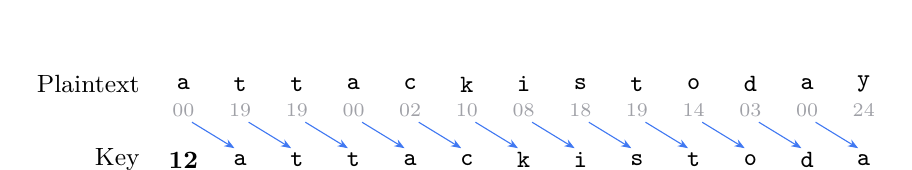
\begin{tikzpicture}[x=7.2mm,y=6mm,font=\small]
  \foreach \l/\v [count=\i] in {a/00,t/19,t/19,a/00,c/02,k/10,i/08,s/18,t/19,o/14,d/03,a/00,y/24}{
    \node (p\i) at (\i,0) {\ttx{\l}};
    \node[gray] at (\i,-0.55) {\scriptsize\v};
  }
  \node[anchor=east] at (0.4,0) {Plaintext};
  \node[anchor=east] at (0.4,-1.6) {Key};
  \node (k1) at (1,-1.6) {\textbf{12}};
  \foreach \l [count=\i] in {a,t,t,a,c,k,i,s,t,o,d,a}{
    \pgfmathtruncatemacro{\j}{\i+1}
    \node (k\j) at (\j,-1.6) {\ttx{\l}};
    \draw[-{Stealth[length=1.3mm]},acc] ($(p\i)+(0.15,-0.8)$) -- ($(k\j)+(-0.1,0.25)$);
  }
\end{tikzpicture}
\end{center}
\begin{center}\small\setlength{\tabcolsep}{3.6pt}
\begin{tabular}{@{}l*{13}{c}@{}}
\toprule
Plaintext & a&t&t&a&c&k&i&s&t&o&d&a&y\\
$P$ & 00&19&19&00&02&10&08&18&19&14&03&00&24\\
Key stream & \textbf{12}&00&19&19&00&02&10&08&18&19&14&03&00\\
$P + k$ & 12&19&\hl{38}&19&02&12&18&\hl{26}&\hl{37}&\hl{33}&17&03&24\\
$C$ & 12&19&12&19&02&12&18&00&11&07&17&03&24\\
Ciphertext & \textbf{M}&\textbf{T}&\textbf{M}&\textbf{T}&\textbf{C}&\textbf{M}&\textbf{S}&\textbf{A}&\textbf{L}&\textbf{H}&\textbf{R}&\textbf{D}&\textbf{Y}\\
\bottomrule
\end{tabular}
\end{center}
Ciphertext: \textbf{\ttx{MTMTCMSALHRDY}}. Each plaintext letter becomes the key one position later (arrows), and the last letter \ttx{y} keys nothing.

\textbf{Brute force.} Eve tries each $k_1$ and unrolls the chain $P_1 = C_1 - k_1$, $P_2 = C_2 - P_1$, \dots:
$k_1 = 11$ gives \ttx{bsuzdjjrunezz}, $k_1 = 13$ gives \ttx{zusbblhtspcbx}, and only $k_1 = 12$ gives readable text, \ttx{attackistoday}. At most 26 trials are needed.
\end{worked}

\subsection{Vernam cipher}
The autokey key is not independent of the message (it \emph{is} the message), so its statistics leak. The next step was taken by \textbf{Gilbert Vernam}, an AT\&T engineer, in \textbf{1918}: use a key stream \textbf{as long as the message} that \textbf{does not repeat} and has no statistical relationship to the plaintext, so that no pattern is left for a statistical attack. Vernam's cipher works on \textbf{binary bits}, not letters, because it was built for teletype machines that send each character as a short binary code. Each plaintext bit is combined with one key bit by exclusive-OR.

\begin{minipage}[c]{0.5\textwidth}
\[
C_i = P_i \oplus K_i \qquad\qquad P_i = C_i \oplus K_i
\]
Here $\oplus$ is XOR: the output is 1 if the two bits differ and 0 if they are equal. Decryption works because XOR undoes itself:
\[
C_i \oplus K_i = P_i \oplus K_i \oplus K_i = P_i \oplus 0 = P_i
\]
\end{minipage}\hfill
\begin{minipage}[c]{0.45\textwidth}
\centering\small
\begin{tabular}{cc|c}
\toprule
$a$ & $b$ & $a\oplus b$\\
\midrule
0&0&0\\ 0&1&1\\ 1&0&1\\ 1&1&0\\
\bottomrule
\end{tabular}
\qquad
\begin{tabular}{@{}r@{\;}l@{}}
$P$ & \ttx{1011}\\
$K$ & \ttx{0110}\\
\midrule
$C$ & \ttx{1101}\\
$C\oplus K$ & \ttx{1011} $= P$
\end{tabular}\\[2pt]
{\footnotesize (bit example is mine, not from the lecture)}
\end{minipage}

XOR is addition modulo 2, so Vernam is the Vigen\`ere idea applied to the two-letter alphabet $\{0, 1\}$: each key bit selects one of two ``Caesar ciphers'' (keep the bit, or flip it). XOR is the natural choice for two reasons. It is its own inverse, so the same operation and the same key stream encrypt and decrypt. And if a key bit is 0 or 1 with probability $\tfrac12$ each, independently of everything else, the ciphertext bit is also 0 or 1 with probability $\tfrac12$ whatever the plaintext bit is, so a single ciphertext bit reveals nothing about the plaintext bit.

\begin{center}
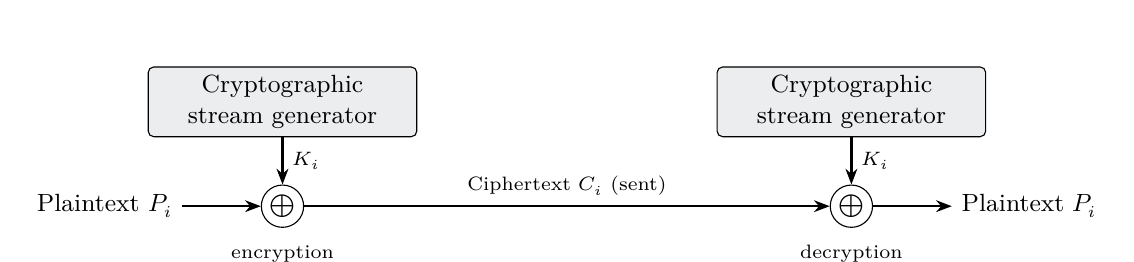
\begin{tikzpicture}[node distance=6mm]
  \node[box,fill=gray!15,text width=32mm] (g1) {Cryptographic stream generator};
  \node[draw,circle,below=6mm of g1,font=\large,inner sep=1pt] (x1) {$\oplus$};
  \node[left=10mm of x1,font=\small] (p1) {Plaintext $P_i$};
  \node[box,fill=gray!15,text width=32mm,right=38mm of g1] (g2) {Cryptographic stream generator};
  \node[draw,circle,below=6mm of g2,font=\large,inner sep=1pt] (x2) {$\oplus$};
  \node[right=10mm of x2,font=\small] (p2) {Plaintext $P_i$};
  \draw[arr] (g1) -- node[right,font=\scriptsize]{$K_i$} (x1);
  \draw[arr] (g2) -- node[right,font=\scriptsize]{$K_i$} (x2);
  \draw[arr] (p1) -- (x1);
  \draw[arr] (x1) -- node[above,font=\scriptsize]{Ciphertext $C_i$ (sent)} (x2);
  \draw[arr] (x2) -- (p2);
  \node[below=1mm of x1,font=\scriptsize] {encryption};
  \node[below=1mm of x2,font=\scriptsize] {decryption};
\end{tikzpicture}
\end{center}
Both sides need the \textbf{same, synchronised key stream}: the receiver's generator must produce exactly the bits the sender used, in the same order.

\textbf{Weakness.} Vernam's machine read the key from a \textbf{loop of paper tape}, so the key eventually \textbf{repeated}, and with enough ciphertext, and some known or probable plaintext, the cipher can be broken. The reason is that whenever two stretches of plaintext are encrypted with the same key bits, the key cancels: $C_1 \oplus C_2 = (P_1 \oplus K) \oplus (P_2 \oplus K) = P_1 \oplus P_2$. For example, with $P_1 = \ttx{10110010}$, $P_2 = \ttx{01100111}$ and $K = \ttx{11010100}$, the ciphertexts are $C_1 = \ttx{01100110}$ and $C_2 = \ttx{10110011}$, and $C_1 \oplus C_2 = \ttx{11010101} = P_1 \oplus P_2$, with no trace of $K$. The XOR of two English texts is full of structure; guessing a probable word in one plaintext reveals the matching part of the other, and then $K = C \oplus P$.
\textbf{Fix:} make the key truly random, as long as the message, and never reused. That is the \textbf{one-time pad} (\S\ref{sec:otp}), which gives perfect secrecy.

\subsection{The classical substitution ciphers compared}
Each cipher in this chapter was designed to remove the weakness that broke the one before it, and the summary below is the usual answer to a ``differentiate'' question.

\begin{mustknow}[: polyalphabetic ciphers]
\textbf{Vigen\`ere:} $C_i = (P_i + K_{i \bmod m}) \bmod 26$, keyword repeated; weakness: the period $m$ (Kasiski, then $m$ Caesar ciphers).
\textbf{Autokey:} key = keyword followed by the plaintext ($k_{i+m} = P_i$; Forouzan: $k_1$, then $k_i = P_{i-1}$); no period, but the key is English, and with a single $k_1$ only 26 keys; one plaintext change alters 2 ciphertext letters.
\textbf{Vernam (1918):} $C_i = P_i \oplus K_i$ on bits, key stream as long as the message; weakness: the tape loop repeats, and reused key bits cancel ($C_1 \oplus C_2 = P_1 \oplus P_2$). Random, never-reused key = one-time pad.
\end{mustknow}

\begin{center}\small\setlength{\tabcolsep}{4pt}
\begin{tabular}{@{}llllll@{}}
\toprule
Cipher & Unit & Key & Keys & Fixed substitute? & Main attack\\
\midrule
Shift (Caesar) & letter & shift $k$ & 25 & yes & brute force\\
Monoalphabetic & letter & permutation & $26!$ & yes & letter frequencies\\
Playfair & digram & $5\times5$ square & $25!$ & per digram & digram frequencies\\
Hill & $m$ letters & invertible $m\times m$ matrix & $< 26^{m^2}$ & per block & known plaintext\\
Vigen\`ere & letter & keyword, repeated & $26^m$ & no (period $m$) & Kasiski + Caesar\\
Autokey & letter & keyword + plaintext & $26^m$ & no (no period) & key is English\\
Vernam & bit & bit stream (tape) & -- & no & reused key stream\\
One-time pad & letter/bit & random, used once & -- & no & none (perfect)\\
\bottomrule
\end{tabular}
\end{center}

\begin{trap}[: the usual slips in Hill and Vigen\`ere answers]
In Hill, state the convention ($C = PK$ with row vectors, or $C = KP$ with columns) and keep it for decryption; check $\gcd(\det K, 26) = 1$ \emph{before} computing the inverse; turn negative entries into $0$--$25$ by adding 26; and always verify $KK^{-1} \equiv I$. In the known-plaintext attack the inverse goes on the left: $K = P^{-1}C$. In Vigen\`ere, remove the spaces first so the keyword runs continuously across words; in autokey, decrypt strictly left to right.
\end{trap}

\begin{fixbox}
\begin{itemize}
  \item The notes put ``key and plaintext share letter frequencies'' under Vigen\`ere cryptanalysis. That point is really about the autokey system, where the key \emph{is} plaintext, so it is placed there above.
  \item Slide L5 (autokey) is correct: \ttx{attackistoday} with $k_1 = 12$ gives \ttx{MTMTCMSALHRDY}; slide L5 (Vigen\`ere, PASCAL) is correct: \ttx{HHWKSWXSLGNTCG} (both checked by script).
\end{itemize}
\end{fixbox}

% Sources: Neso videos (one-time pad, rail fence, row-column transposition; notes5.md), college Lecture 5 slides 54-55,
% Stallings 2.2-2.3, Forouzan 3.2. Every number recomputed by script (scratchpad/r3/verify.py).
\providecommand{\railfence}[1]{%
  \foreach \l/\r [count=\i] in {#1}{\node[font=\small] (rf\i) at (\i*0.5,-\r*0.6) {\l};}}

\section{One-Time Pad \hot}\label{sec:otp}
\asked{Mid-sem 2025--26 Q1 (8 marks): OTP-Vigen\`ere with key stream 9 0 1 7 23 15 21 14 11 11 2 8 9 (Stallings 2.x). Part (b), finding a key that maps the ciphertext to another plaintext, is exactly why an OTP is unbreakable: every plaintext of the same length is possible.}

\subsection{How it grew out of the earlier ciphers}
Every substitution cipher so far was broken through the same flaw: the key is reused, so some regularity of the plaintext survives into the ciphertext. A monoalphabetic cipher applies one fixed substitution to the whole message, so the letter frequencies of English pass straight through. Vigen\`ere rotates through $m$ substitutions, so once $m$ is known the ciphertext splits into $m$ interleaved Caesar ciphers (\S\ref{sec:classextra} shows how the Kasiski test finds $m$). The autokey cipher removes the period by continuing the key with the plaintext itself, but then the key is English text and carries English statistics. Vernam's cipher (1918) works on bits with a long key stream punched on paper tape, but the tape was a loop, so the key eventually repeated and a long enough message could be broken.

Shannon's study of secrecy showed what the key must look like for \emph{no} regularity to survive: each plaintext symbol must be encrypted with a key symbol chosen \textbf{at random from the whole key domain}, independently of every other symbol. Even the weak additive cipher becomes perfect under this rule. It is broken easily because the same shift is used for every letter; but if the first letter is shifted by 04, the second by 02, the third by 21, and each shift is drawn at random from $00, 01, \dots, 25$, then nothing links one ciphertext letter to another or to the plaintext. This is the \textbf{one-time pad} (OTP), the last substitution technique of the course and an improvement to the Vernam cipher (Stallings credits the improvement to Joseph Mauborgne; Forouzan's slides credit Vernam).

\begin{center}\small
\begin{tabularx}{\textwidth}{@{}l X X@{}}
\toprule
Cipher & Key & What goes wrong\\
\midrule
Vigen\`ere & short keyword, \textbf{repeated} & repeats every $m$ letters $\Rightarrow$ split into Caesar ciphers\\
Autokey & keyword + plaintext & key is English $\Rightarrow$ has English letter frequencies\\
Vernam & long key stream (paper tape) & tape loops, so the key \textbf{eventually repeats}\\
\textbf{One-time pad} & \textbf{truly random}, \textbf{same length} as message, \textbf{used once} & nothing to exploit\\
\bottomrule
\end{tabularx}
\end{center}

\subsection{Definition and mechanism}
In a one-time pad the key is a \textbf{truly random} sequence that is \textbf{as long as the message}, so it never has to be repeated. The key is used to encrypt and decrypt \textbf{a single message} and is then \textbf{discarded}; every new message needs a new random key of its own length. The encryption rule itself is unchanged from Vigen\`ere (letters) or Vernam (bits): only the key is different. Stallings calls the result ``the ultimate in security'', because such a scheme is unbreakable.

\begin{mustknow}[: one-time pad]
\textbf{Key}: truly random, same length as the message, used once, then destroyed.\\[2pt]
\textbf{Letters}: $C_i = (P_i + K_i) \bmod 26$, \;$P_i = (C_i - K_i) \bmod 26$. \qquad \textbf{Bits}: $C_i = P_i \oplus K_i$, \;$P_i = C_i \oplus K_i$.\\[2pt]
\textbf{Perfect secrecy}: $\Pr[M \mid C] = \Pr[M]$; the ciphertext reveals nothing about the plaintext. The OTP is the \emph{only} cipher with this property (key at least as long as the message is necessary).\\[2pt]
\textbf{Two difficulties}: (1) making large quantities of random keys; (2) key distribution and protection.
\end{mustknow}

Decryption recovers the plaintext because the key cancels: $(P_i + K_i) - K_i \equiv P_i \pmod{26}$, and $(P_i \oplus K_i) \oplus K_i = P_i \oplus 0 = P_i$, since XOR of a bit with itself is 0. The receiver therefore needs exactly the same key, in the same order, aligned with the same letter positions; this requirement is the source of all the practical difficulties discussed below.

\subsection{Example 1: letters}
Plaintext \ttx{attackatdawn}, random key \ttx{qvhzmxkbplwe} (12 key letters for 12 plaintext letters). Each letter is shifted by its own key value, and four sums pass 25 and wrap:
\begin{center}\small\setlength{\tabcolsep}{4.5pt}
\begin{tabular}{@{}l*{12}{c}@{}}
\toprule
Plain & a&t&t&a&c&k&a&t&d&a&w&n\\
$P$ & 0&19&19&0&2&10&0&19&3&0&22&13\\
Key & q&v&h&z&m&x&k&b&p&l&w&e\\
$K$ & 16&21&7&25&12&23&10&1&15&11&22&4\\
$P+K$ & 16&\hl{40}&\hl{26}&25&14&\hl{33}&10&20&18&11&\hl{44}&17\\
$\bmod 26$ & 16&14&0&25&14&7&10&20&18&11&18&17\\
Cipher & \textbf{Q}&\textbf{O}&\textbf{A}&\textbf{Z}&\textbf{O}&\textbf{H}&\textbf{K}&\textbf{U}&\textbf{S}&\textbf{L}&\textbf{S}&\textbf{R}\\
\bottomrule
\end{tabular}
\end{center}
Ciphertext \textbf{\ttx{QOAZOHKUSLSR}}. The receiver computes $(C - K) \bmod 26$ letter by letter to get \ttx{attackatdawn} back, then destroys the key. The two \ttx{t}'s of \ttx{att} became \ttx{O} and \ttx{A}, and the two \ttx{S}'s of the ciphertext came from different letters (\ttx{d} and \ttx{w}): equal letters do not produce equal letters, and equal ciphertext letters do not mean equal plaintext letters.

\subsection{Example 2: bits}
``HI'' in 8-bit ASCII, XORed with a random 16-bit key. Each ciphertext bit is 1 exactly where the plaintext bit and the key bit differ:
\begin{center}\small\ttfamily
\begin{tabular}{@{}r@{\quad}l@{\quad}l@{}}
\rmfamily Plaintext (H, I) & 01001000 & 01001001\\
\rmfamily Key & 10110101 & 01101100\\
\midrule
\rmfamily Ciphertext $P\oplus K$ & 11111101 & 00100101\\
\rmfamily $C \oplus K$ & 01001000 & 01001001 \rmfamily\;= ``HI'' again\\
\end{tabular}
\end{center}

\subsection{Why it cannot be broken}
The one-time pad produces random output that has \textbf{no statistical relationship to the plaintext}. Since the ciphertext contains no information whatsoever about the plaintext, there is simply no way to break the code, and the security of the scheme comes \textbf{entirely from the randomness of the key}. This can be seen at three levels.

\textbf{One letter.} Suppose the attacker sees the ciphertext letter \ttx{Q} ($= 16$). Every plaintext letter could have produced it, each with exactly one key letter, namely $K = (16 - P) \bmod 26$:
\begin{center}\small\setlength{\tabcolsep}{5pt}
\begin{tabular}{@{}l*{7}{c}@{}}
\toprule
If the plaintext was & a & b & c & d & e & \dots & z\\
then the key was & q & p & o & n & m & \dots & r\\
\bottomrule
\end{tabular}
\end{center}
Since the key letter was drawn at random, all 26 cases are \textbf{equally likely}, and seeing \ttx{Q} tells the attacker nothing. The same argument shows that the ciphertext letters themselves are uniformly distributed: $\Pr[C_i = c] = \sum_p \Pr[P_i = p] \cdot \Pr[K_i = c - p] = \sum_p \Pr[P_i = p] \cdot \tfrac{1}{26} = \tfrac{1}{26}$, whatever the plaintext statistics. The ciphertext has a flat frequency histogram (no peak for \ttx{e} to aim at), and since the key never repeats, the Kasiski and index-of-coincidence tests of \S\ref{sec:classextra} find nothing.

\textbf{The whole message.} For a message of $n$ letters there are $26^n$ keys, exactly as many as there are $n$-letter strings, and every string is the decryption of the ciphertext under exactly one key. The same ciphertext therefore decrypts to anything of the same length:
\begin{center}\small
\begin{tabular}{@{}lll@{}}
\toprule
Ciphertext & Key tried & Result\\
\midrule
\ttx{QOAZOHKUSLSR} & \ttx{qvhzmxkbplwe} & \textbf{attack at dawn}\\
\ttx{QOAZOHKUSLSR} & \ttx{zkhikhruztku} & \textbf{retreat at six}\\
\ttx{KXFUDM} & \ttx{kemubc} & \textbf{attack}\\
\ttx{KXFUDM} & \ttx{htaqqj} & \textbf{defend}\\
\bottomrule
\end{tabular}
\end{center}
A brute-force search produces \emph{every} meaningful message of that length, with nothing to say which one was sent. Compare the Caesar cipher, where only one of the 25 tries makes sense (GERMANY): there the key space is far smaller than the message space, so wrong keys give gibberish and the right one stands out.

\subsection{Perfect secrecy: the derivation}
\textbf{Definition (Shannon, 1949).} A cipher has \textbf{perfect secrecy} if, for every plaintext $M$ and every ciphertext $C$ that can occur,
\[
\Pr[M \mid C] = \Pr[M].
\]
$\Pr[M]$ is what the attacker believes about the message before interception (for example, that ``no attack today'' is the usual message), and $\Pr[M \mid C]$ is what she believes after seeing $C$. Equality means the ciphertext changes nothing: \imp{given a ciphertext from a perfectly secure cipher, absolutely nothing is revealed about the plaintext.}

\textbf{The one-time pad meets the definition.} Fix any plaintext $M$ and ciphertext $C$ of length $n$. Exactly one key maps $M$ to $C$, namely $K = C - M \pmod{26}$ letter by letter (or $K = C \oplus M$ for bits). Every key is equally likely, with probability $1/26^n$, so
\[
\Pr[C \mid M] = \Pr[K = C - M] = \frac{1}{26^n}\quad\text{for every } M .
\]
Averaging over the messages, $\Pr[C] = \sum_{M} \Pr[M]\Pr[C \mid M] = \frac{1}{26^n}\sum_M \Pr[M] = \frac{1}{26^n}$. Bayes' rule then gives
\[
\Pr[M \mid C] = \frac{\Pr[C \mid M]\,\Pr[M]}{\Pr[C]} = \frac{(1/26^n)\,\Pr[M]}{1/26^n} = \Pr[M].
\]
In words: every key is equally likely, and for each candidate plaintext exactly one key turns it into the observed $C$, so $C$ ``points'' equally strongly to every plaintext, and the attacker's probabilities stay where they were. For a one-bit pad with $\Pr[M = 0] = 0.9$: $\Pr[C = 1] = 0.9 \cdot 0.5 + 0.1 \cdot 0.5 = 0.5$, and $\Pr[M = 0 \mid C = 1] = 0.5 \cdot 0.9 / 0.5 = 0.9$; Eve's best guess after interception is exactly her guess before it.

\textbf{Why the key must be as long as the message.} Suppose there were fewer keys than possible messages. Decrypting a given $C$ under all keys yields at most as many candidate plaintexts as there are keys, so some message $M$ with $\Pr[M] > 0$ is not among them and has $\Pr[M \mid C] = 0$: the ciphertext has ruled it out, and secrecy is not perfect. For example, a Caesar shift used for a two-letter message cannot turn \ttx{aa} into \ttx{AB}, because one shift maps equal letters to equal letters; seeing \ttx{AB} eliminates \ttx{aa}, \ttx{bb}, \dots. Hence perfect secrecy needs at least as many keys as messages, i.e.\ at least as much random key as message. This is Shannon's bound, and it is the reason the OTP is the \textbf{only} practical cipher with perfect secrecy.

\textbf{Unconditional versus computational security.} Perfect secrecy is the \textbf{unconditionally secure} case of \S\ref{sec:schemes}: no amount of ciphertext or computing power helps, because the information is simply not there. Every other cipher in this course (DES, AES, RSA, \dots) is only \textbf{computationally} secure: it can be broken in principle, but doing so costs more time or money than the information is worth.

\begin{trap}[: what perfect secrecy does not give]
The OTP hides the \emph{content} among messages of the \emph{same length}; it does not hide the length (if Alice's answer is ``YES'' or ``NO'', a 3-letter ciphertext gives it away). It also gives no integrity: flipping a ciphertext bit flips the same plaintext bit, and Bob cannot detect it. Integrity needs a hash or MAC (\S\ref{sec:integrity}).
\end{trap}

\subsection{The rules, and what breaks if you bend them}
\textbf{Rule 1: never reuse a key (the ``two-time pad'').} Encrypt a second message \ttx{holdposition} with the \emph{same} key \ttx{qvhzmxkbplwe}; the result is $C_2 = $ \ttx{XJSCBLCJITKR}. Subtracting the two ciphertexts cancels the key,
\[
C_1 - C_2 = (P_1 + K) - (P_2 + K) = P_1 - P_2 \pmod{26},
\]
and indeed both differences equal \ttx{TFIXNWILKSIA}. What remains is two English texts combined with each other, which has strong structure (common words, frequent letters) that the attacker can attack without knowing any key. Worse, if the attacker knows or guesses $P_1$ (``attack at dawn'' is a stock phrase), she recovers the key $K = C_1 - P_1 = $ \ttx{qvhzmxkbplwe} and then $P_2 = C_2 - K = $ \textbf{hold position}. With bits the same cancellation is $C_1 \oplus C_2 = P_1 \oplus P_2$. Historically, Soviet pads that were reused in the 1940s were partly read by the US VENONA project for exactly this reason.

\textbf{Rule 2: the key must be truly random.} If the key is text taken from a book (a \textbf{running key}), it has English letter frequencies and can be attacked like the autokey. If it is generated by a formula from a short seed, the cipher is really a stream cipher: at best \emph{computationally} secure, never perfect, because the number of possible key streams is only the number of seeds.

\textbf{Rule 3: the key must be at least as long as the message.} A shorter key has to repeat, and then the cipher is back to Vigen\`ere or Vernam with their weaknesses; the derivation above shows that perfect secrecy is then impossible.

\textbf{Known plaintext does not hurt a correctly used OTP.} If the attacker learns one plaintext and its ciphertext, she gets $K = C - P$, but only for that message, and that key is never used again. For every other cipher a known pair helps break future traffic (\S\ref{sec:classextra}); here it is worthless.

\subsection{Two fundamental difficulties}
In theory the one-time pad is the end of the story; in practice it has two fundamental difficulties.
\begin{enumerate}[leftmargin=1.5em]
  \item \imp{The practical problem of making large quantities of random keys.} Every message needs fresh random key material of the same size, so a system carrying a lot of traffic needs millions of truly random characters on a regular basis. Pseudorandom generators do not qualify (Rule 2), and good physical sources of randomness are slow.
  \item \imp{Even more daunting is the problem of key distribution and protection.} For every message, sender and receiver must hold an identical key of the same length, delivered and stored securely, and destroyed after use. If a secure channel able to carry that much key existed, the message could simply be sent over it instead.
\end{enumerate}
The second point is softened by \emph{timing}: the key can be carried in advance, by a trusted courier, at a moment and by a route the parties choose, after which the messages can travel over any insecure channel. The slide's example is a president who sends a trusted envoy with a random key to another president before sending a completely secret message. This is why Forouzan calls the OTP ``a perfect cipher, but almost impossible to implement commercially''.

\textbf{Advantages.} Perfect secrecy: no attack, however much ciphertext or computing power the attacker has, can extract information about the plaintext. Encryption and decryption are trivial additions or XORs. \textbf{Disadvantages.} The key is as long as all the traffic ever sent, must be truly random, must reach the receiver securely in advance and must never be reused; it gives no integrity. Because of these difficulties, \imp{the one-time pad is of limited utility, and is useful primarily for low-bandwidth channels requiring very high security} (diplomatic and military links).

\subsection{Exam-format one-time-pad numerical}
\begin{worked}[: Stallings 2.x, mid-sem 2025--26 Q1]
\textbf{Q.} This problem uses a one-time pad version of the Vigen\`ere cipher: each plaintext letter is shifted by the next number of the key stream \ttx{9 0 1 7 23 15 21 14 11 11 2 8 9}. (a) Encrypt \ttx{sendmoremoney}. (b) Using the ciphertext from (a), find a key stream that makes it decrypt to \ttx{cashnotneeded}. (8 marks)

\textbf{(a)} $C_i = (P_i + K_i) \bmod 26$, letters numbered from $a = 0$:
\begin{center}\small\setlength{\tabcolsep}{4pt}
\begin{tabular}{@{}l*{13}{c}@{}}
\toprule
Plain & s&e&n&d&m&o&r&e&m&o&n&e&y\\
$P$ & 18&4&13&3&12&14&17&4&12&14&13&4&24\\
$K$ & 9&0&1&7&23&15&21&14&11&11&2&8&9\\
$P{+}K$ & \hl{27}&4&14&10&\hl{35}&\hl{29}&\hl{38}&18&23&25&15&12&\hl{33}\\
mod 26 & 1&4&14&10&9&3&12&18&23&25&15&12&7\\
Cipher & \textbf{B}&\textbf{E}&\textbf{O}&\textbf{K}&\textbf{J}&\textbf{D}&\textbf{M}&\textbf{S}&\textbf{X}&\textbf{Z}&\textbf{P}&\textbf{M}&\textbf{H}\\
\bottomrule
\end{tabular}
\end{center}
Ciphertext: \textbf{\ttx{BEOKJDMSXZPMH}}.

\textbf{(b)} The key that turns $C$ into a chosen plaintext $P'$ is $K'_i = (C_i - P'_i) \bmod 26$:
\begin{center}\small\setlength{\tabcolsep}{3.6pt}
\begin{tabular}{@{}l*{13}{c}@{}}
\toprule
$C$ & B 1&E 4&O 14&K 10&J 9&D 3&M 12&S 18&X 23&Z 25&P 15&M 12&H 7\\
$P'$ & c 2&a 0&s 18&h 7&n 13&o 14&t 19&n 13&e 4&e 4&d 3&e 4&d 3\\
$C - P'$ & $-1$&4&$-4$&3&$-4$&$-11$&$-7$&5&19&21&12&8&4\\
$K'$ & \textbf{25}&\textbf{4}&\textbf{22}&\textbf{3}&\textbf{22}&\textbf{15}&\textbf{19}&\textbf{5}&\textbf{19}&\textbf{21}&\textbf{12}&\textbf{8}&\textbf{4}\\
\bottomrule
\end{tabular}
\end{center}
Key stream: \textbf{25 4 22 3 22 15 19 5 19 21 12 8 4}. Check, first letter: $(2 + 25) \bmod 26 = 1 = $ \ttx{B} \checkmark.

\textbf{Conclusion to write.} The same ciphertext decrypts to \ttx{sendmoremoney} under one key and to \ttx{cashnotneeded} under another, and both keys are equally likely random streams. An attacker who tries all keys gets every 13-letter message and cannot tell which was sent, so the one-time pad cannot be broken by brute force: it has perfect secrecy.
\end{worked}

\section{Transposition Ciphers}\label{sec:transp}
Substitution ciphers replace letters, and every one of them up to the one-time pad was attacked through the statistics of the replaced letters. A \textbf{transposition cipher} takes the opposite approach: some sort of \textbf{permutation is applied to the plaintext letters}. The letters themselves are \textbf{not replaced}; only their \textbf{positions} change, so a symbol in the first position of the plaintext may appear in the tenth position of the ciphertext. A \textbf{permutation} of $n$ positions is a rearrangement in which every position receives exactly one letter; there are $n!$ of them, and the key of a transposition cipher is a permutation or a rule (depth, column order) that generates one.

\textbf{Why transposition keeps the letter frequencies.} Every plaintext letter appears in the ciphertext exactly once, merely at another position, so the ciphertext is an \emph{anagram} of the plaintext: the two contain the same letters the same number of times, and their single-letter frequencies are identical. (Script check: the ciphertext of the Kill Corona example below has exactly the letter counts of its padded plaintext.) This gives the cryptanalyst an immediate test. If a ciphertext is unreadable but its letter counts look like normal English (\ttx{e} about 12.7\%, \ttx{t} 9.1\%, \ttx{a} 8.2\%, and \ttx{j}, \ttx{q}, \ttx{x}, \ttx{z} almost absent), the letters are genuine and only their order is scrambled: the cipher is a \textbf{transposition}. A monoalphabetic substitution shows the same \emph{shape} of histogram but on the wrong letters (the tallest bar is not \ttx{e}), and a polyalphabetic cipher flattens it. The frequency count identifies a transposition but does not break it; the attacker still has to find the order, using digram statistics (\ttx{th}, \ttx{he}, \ttx{in}, \dots) to decide which letters belong next to each other. The simplest transposition is the rail fence.

\begin{mustknow}[: transposition]
Substitution changes the \emph{letters}; transposition changes their \emph{positions}, so \textbf{letter frequencies are preserved} (a frequency count that looks like plain English means transposition).\\
Rail fence, depth $D$: zig-zag with period $2(D-1)$, read row by row. Row--column: write row by row, read column by column, \textbf{key = order of the columns}; two stages = do it again on the ciphertext.
\end{mustknow}

\subsection{Rail fence}
In the rail fence technique the plaintext is \textbf{written down as a sequence of diagonals and then read off as a sequence of rows}. The letters are written on $D$ rows (the \textbf{depth}), moving down one row per letter from row 1 to row $D$ and then back up to row 1, in a zig-zag; spaces and punctuation are dropped. The ciphertext is row 1, followed by row 2, and so on. Going down takes $D - 1$ steps and coming back takes $D - 1$ steps, so the row pattern repeats every $2(D-1)$ letters.

\textbf{Example:} ``neso academy is the best'', depth 2 (20 letters):
\begin{center}
\begin{tikzpicture}
  \railfence{n/0,e/1,s/0,o/1,a/0,c/1,a/0,d/1,e/0,m/1,y/0,i/1,s/0,t/1,h/0,e/1,b/0,e/1,s/0,t/1}
  \foreach \i in {1,...,19}{\pgfmathtruncatemacro{\j}{\i+1}\draw[gray!50] (rf\i) -- (rf\j);}
  \node[font=\scriptsize,anchor=east] at (0.2,0) {row 1};
  \node[font=\scriptsize,anchor=east] at (0.2,-0.6) {row 2};
\end{tikzpicture}
\end{center}
Row 1: \ttx{NSAAEYSHBS}\quad Row 2: \ttx{EOCDMITEET}\quad $\Rightarrow$\quad \textbf{\ttx{NSAAEYSHBSEOCDMITEET}}

\textbf{Depth 3}, ``Thank you very much'' (16 letters). The path visits rows 1, 2, 3, 2, 1, 2, 3, \dots\ and repeats every $2(D-1) = 4$ letters:
\begin{center}
\begin{tikzpicture}
  \railfence{t/0,h/1,a/2,n/1,k/0,y/1,o/2,u/1,v/0,e/1,r/2,y/1,m/0,u/1,c/2,h/1}
  \foreach \i in {1,...,15}{\pgfmathtruncatemacro{\j}{\i+1}\draw[gray!50] (rf\i) -- (rf\j);}
\end{tikzpicture}
\end{center}
Rows: \ttx{TKVM} + \ttx{HNYUEYUH} + \ttx{AORC} $\Rightarrow$ \textbf{\ttx{TKVMHNYUEYUHAORC}}. The middle row holds twice as many letters as the outer rows, because the zig-zag passes through it on the way down and again on the way up.

\textbf{Homework} (``neso academy is the best'', depth 3): the rows are \ttx{NAESB}, \ttx{EOCDMITEET} and \ttx{SAYHS}, so the ciphertext is \textbf{\ttx{NAESBEOCDMITEETSAYHS}}.

\textbf{Security.} The only secret is the depth, and it can only be one of $2, 3, \dots, L - 1$ for an $L$-letter message, so an attacker simply tries every depth; the frequencies are English, which tells her at once that she is facing a transposition. The rail fence is therefore a scrambling rule rather than a real cipher (Forouzan files it under \emph{keyless} transpositions, \S\ref{sec:classextra}).

\subsection{Decrypting a rail fence}
The receiver knows the depth $D$. The difficulty is that the ciphertext does not show where one row ends and the next begins, so the first job is to work out \textbf{how many letters each row holds}; after that the zig-zag can be rebuilt and read along its path.
\begin{enumerate}[leftmargin=1.5em]
  \item Count the letters $L$. The zig-zag pattern of rows repeats every $2(D-1)$ letters.
  \item Write the \textbf{row number of every position} (1, 2, \dots, $D$, \dots, 2, 1, 2, \dots) and \textbf{count} how many times each row appears.
  \item \textbf{Cut} the ciphertext into pieces of those lengths: the first piece is row 1, the next is row 2, and so on.
  \item Put each piece back into its row's positions, left to right. Then \textbf{read along the zig-zag} (position 1, 2, 3, \dots).
\end{enumerate}
\textbf{The counts without writing the pattern.} Write $L = q \cdot 2(D-1) + r$ with $0 \le r < 2(D-1)$. Each complete cycle visits row 1 and row $D$ once and every middle row twice, and within a cycle row $i$ is visited at positions $i$ and $2D - i$. So row 1 holds $q + [r \ge 1]$ letters, row $D$ holds $q + [r \ge D]$, and a middle row $i$ holds $2q + [r \ge i] + [r \ge 2D - i]$, where $[\cdot]$ is 1 if the condition holds and 0 otherwise. For $L = 17$, $D = 4$: $17 = 2 \cdot 6 + 5$, giving $3, 5, 6, 3$, as in Example 3 below.

\textbf{Example 1: depth 2.} \ttx{NSAAEYSHBSEOCDMITEET} (20 letters). The pattern is 1 2 1 2 \dots, so each row has 10 letters:
row 1 $=$ \ttx{NSAAEYSHBS}, row 2 $=$ \ttx{EOCDMITEET}. Take letters alternately from row 1 and row 2:
\ttx{N}\textbf{\ttx{E}}\ttx{S}\textbf{\ttx{O}}\ttx{A}\textbf{\ttx{C}}\dots\ $\Rightarrow$ \textbf{nesoacademyisthebest}.
(Depth-2 shortcut: split in half and interleave. With an odd length, row 1 gets the extra letter.)

\textbf{Example 2: depth 3.} \ttx{TKVMHNYUEYUHAORC} (16 letters). The pattern repeats every $2(3-1) = 4$:
\begin{center}\small\setlength{\tabcolsep}{4pt}
\begin{tabular}{@{}l*{16}{c}@{}}
\toprule
Position & 1&2&3&4&5&6&7&8&9&10&11&12&13&14&15&16\\
Row & 1&2&3&2&1&2&3&2&1&2&3&2&1&2&3&2\\
\bottomrule
\end{tabular}
\end{center}
Row 1 appears 4 times, row 2 8 times, row 3 4 times. Cut: \ttx{TKVM | HNYUEYUH | AORC}.
Fill the row-1 positions (1, 5, 9, 13) with T K V M, the row-2 positions with H N Y U E Y U H, and the row-3 positions with A O R C. Reading positions 1 to 16 gives \textbf{thankyouverymuch}.

\textbf{Example 3: depth 4, unequal rows} (the tricky case). \ttx{CGIRORYSYTAHFNPPU} (17 letters). The pattern repeats every $2(4-1) = 6$:
\begin{center}\small\setlength{\tabcolsep}{4pt}
\begin{tabular}{@{}l*{17}{c}@{}}
\toprule
Position & 1&2&3&4&5&6&7&8&9&10&11&12&13&14&15&16&17\\
Row & 1&2&3&4&3&2&1&2&3&4&3&2&1&2&3&4&3\\
\bottomrule
\end{tabular}
\end{center}
Counts: row 1 $= 3$, row 2 $= 5$, row 3 $= 6$, row 4 $= 3$ (total 17 \checkmark). Cut: \ttx{CGI | RORYS | YTAHFN | PPU}. Put the pieces back:
\begin{center}
\begin{tikzpicture}
  \railfence{C/0,R/1,Y/2,P/3,T/2,O/1,G/0,R/1,A/2,P/3,H/2,Y/1,I/0,S/1,F/2,U/3,N/2}
  \foreach \i in {1,...,16}{\pgfmathtruncatemacro{\j}{\i+1}\draw[gray!50] (rf\i) -- (rf\j);}
  \node[font=\scriptsize,anchor=east] at (0.2,0) {row 1: CGI};
  \node[font=\scriptsize,anchor=east] at (0.2,-0.6) {row 2: RORYS};
  \node[font=\scriptsize,anchor=east] at (0.2,-1.2) {row 3: YTAHFN};
  \node[font=\scriptsize,anchor=east] at (0.2,-1.8) {row 4: PPU};
\end{tikzpicture}
\end{center}
Read along the line: \textbf{cryptographyisfun} (``cryptography is fun''). The same steps, with row counts 5, 10, 5, turn the homework answer above back into \ttx{nesoacademyisthebest}.

\begin{trap}[: unequal rows]
Do not assume the rows are equal, or that the middle rows are equal to each other. In Example 3 rows 2 and 3 have different lengths (5 and 6) because the message stops partway through a cycle, after the zig-zag has passed row 3 on its way up but before it reaches row 2.
\end{trap}

\subsection{Row--column transposition}
The rail fence has too few keys to be of any use. A more complex scheme uses a \textbf{rectangle}: the message is \textbf{written row by row} into a rectangle of $c$ columns and \textbf{read column by column}, but the columns are read in a \textbf{secret order}. The \textbf{key} is that order of the columns, written as a number above each column (the column marked 1 is read first). Leftover cells in the last row are filled with agreed filler letters (\ttx{x}, \ttx{y}, \ttx{z}), so that every column has the same height and the receiver can remove the fillers after decryption.

\textbf{Example:} ``Kill Corona Virus at twelve am tomorrow'' (33 letters), 7 columns $\times$ 5 rows = 35 cells, so 2 fillers (\ttx{y}, \ttx{z}). Key \textbf{4 3 1 2 5 6 7}.
\begin{center}\small
\begin{minipage}[c]{0.4\textwidth}\centering
\begin{tabular}{|*{7}{c|}}
\multicolumn{1}{c}{4}&\multicolumn{1}{c}{3}&\multicolumn{1}{c}{\textbf{1}}&\multicolumn{1}{c}{2}&\multicolumn{1}{c}{5}&\multicolumn{1}{c}{6}&\multicolumn{1}{c}{7}\\
\hline
k&i&\cellcolor{warn!18}l&l&c&o&r\\ \hline
o&n&\cellcolor{warn!18}a&v&i&r&u\\ \hline
s&a&\cellcolor{warn!18}t&t&w&e&l\\ \hline
v&e&\cellcolor{warn!18}a&m&t&o&m\\ \hline
o&r&\cellcolor{warn!18}r&o&w&\textit{y}&\textit{z}\\ \hline
\end{tabular}\\[2pt]
{\footnotesize numbers above = read order}
\end{minipage}
\begin{minipage}[c]{0.5\textwidth}
\begin{tabular}{@{}lll@{}}
\toprule
Order & Column & Letters\\
\midrule
1 & col 3 & LATAR\\
2 & col 4 & LVTMO\\
3 & col 2 & INAER\\
4 & col 1 & KOSVO\\
5 & col 5 & CIWTW\\
6 & col 6 & OREOY\\
7 & col 7 & RULMZ\\
\bottomrule
\end{tabular}
\end{minipage}
\end{center}
Answer: \textbf{\ttx{LATARLVTMOINAERKOSVOCIWTWOREOYRULMZ}}

\textbf{Key space and weakness.} With $c$ columns there are $c!$ reading orders ($7! = 5040$ here), multiplied by the choice of $c$, so brute force by hand is already tedious. The weakness is structural. Consecutive ciphertext letters come from one column, i.e.\ from plaintext positions exactly $c$ apart: the first five ciphertext letters are plaintext letters 3, 10, 17, 24, 31. An attacker who guesses the number of rows (here 5, a divisor of 35) cuts the ciphertext into 5-letter pieces, stands them side by side as columns and rearranges the columns until the rows read as English, guided by common digrams; Forouzan calls this the \textbf{pattern attack} (\S\ref{sec:classextra}). This is why the lecture says a single transposition ``can be reconstructed''.

\begin{worked}[: decrypting a row--column transposition]
\textbf{Q.} Decrypt \ttx{LATARLVTMOINAERKOSVOCIWTWOREOYRULMZ}, written row by row into 7 columns and read in the column order \textbf{4 3 1 2 5 6 7}.

\textbf{Column height.} $L = 35$ letters in 7 columns, so every column holds $35 / 7 = 5$ letters (5 rows).

\textbf{Refill the columns in key order.} The first 5 letters belong to the column numbered 1 (column 3), the next 5 to the column numbered 2 (column 4), and so on:
\begin{center}\small
\begin{tabular}{@{}llllllll@{}}
\toprule
Piece & LATAR & LVTMO & INAER & KOSVO & CIWTW & OREOY & RULMZ\\
Goes to column & 3 & 4 & 2 & 1 & 5 & 6 & 7\\
\bottomrule
\end{tabular}
\end{center}
\textbf{Read row by row.} Column 1 is now \ttx{KOSVO}, column 2 \ttx{INAER}, column 3 \ttx{LATAR}, and so on; reading the rebuilt grid across its rows gives \ttx{killcor | onaviru | sattwel | veamtom | orrowyz}. Removing the fillers \ttx{yz}, the plaintext is \textbf{kill corona virus at twelve am tomorrow}. Check: re-encrypting gives the received ciphertext \checkmark.
\end{worked}

\subsection{Two stages: more complex}
A single transposition leaves the regular pattern just described. The remedy is to \textbf{feed the ciphertext back in} and transpose again, usually with the same key:
\begin{center}\small
\begin{minipage}[c]{0.4\textwidth}\centering
\begin{tabular}{|*{7}{c|}}
\multicolumn{1}{c}{4}&\multicolumn{1}{c}{3}&\multicolumn{1}{c}{\textbf{1}}&\multicolumn{1}{c}{2}&\multicolumn{1}{c}{5}&\multicolumn{1}{c}{6}&\multicolumn{1}{c}{7}\\
\hline
L&A&\cellcolor{warn!18}T&A&R&L&V\\ \hline
T&M&\cellcolor{warn!18}O&I&N&A&E\\ \hline
R&K&\cellcolor{warn!18}O&S&V&O&C\\ \hline
I&W&\cellcolor{warn!18}T&W&O&R&E\\ \hline
O&Y&\cellcolor{warn!18}R&U&L&M&Z\\ \hline
\end{tabular}
\end{minipage}
\begin{minipage}[c]{0.5\textwidth}
Read columns 3, 4, 2, 1, 5, 6, 7:\\[2pt]
\ttx{TOOTR AISWU AMKWY LTRIO RNVOL LAORM VECEZ}
\end{minipage}
\end{center}
Answer: \textbf{\ttx{TOOTRAISWUAMKWYLTRIORNVOLLAORMVECEZ}}.
The full key is now: the rectangle size, the column order and the number of stages. To decrypt, the receiver applies the single-stage decryption of the worked example twice (the second stage is undone first).

\textbf{Why two stages are stronger.} After one stage, ciphertext positions 1--5 hold plaintext letters $3, 10, 17, 24, 31$: a run with constant step 7. After two stages they hold plaintext letters $17, 32, 8, 26, 7$ (computed by composing the two permutations), and no constant step appears anywhere in the ciphertext. Cutting the ciphertext into columns therefore no longer produces fragments of plaintext rows, and the attacker must undo both permutations at once instead of one rectangle at a time. Two stages are still a single permutation of the 35 positions (so the letter frequencies are still those of English), but it is not a \emph{columnar} permutation: it lies outside the small, regular family that the pattern attack searches. \S\ref{sec:classextra} repeats this analysis on Forouzan's keyed columnar example.

\begin{fixbox}
\begin{itemize}
  \item ``Thank you very much'', depth 3, is \ttx{TKVMHNYUEYUH}\textbf{\ttx{AORC}}. The notes' final string ends in \ttx{AORE}, but their own row reading gives \ttx{AORC}.
  \item Row--column: the speaker says ``R U L M C'' for column 7, but the grid (and slide) give \ttx{RULMZ}. All other results were checked by script and are correct.
  \item The OTP formulas, Shannon and $P(M\mid C) = P(M)$ come from Gemini's notes, not the slides. They are standard and correct.
\end{itemize}
\end{fixbox}

% College Lecture 5 topics not in the Neso videos: multiplicative/affine and its attack, cryptanalysis of Vigenere
% (Kasiski, index of coincidence) and Hill, rotor/Enigma, keyless/keyed/columnar transposition, stream vs block.
% Sources: Lecture 5 slides (scanned; OCR in scratchpad/r3/l5.txt), Forouzan ch. 3, Stallings ch. 2-3.
% Every number recomputed by script (scratchpad/r3/verify2.py, kas2.py).
\section{Traditional Ciphers: Remaining Topics (Lecture 5)}\label{sec:classextra}
The college lecture follows Forouzan's chapter 3, which treats the classical ciphers as arithmetic in $\mathbb{Z}_{26}$ (letters $a = 0, \dots, z = 25$) and pays more attention to how each cipher is \emph{broken}. This section collects what the Neso videos did not cover: the multiplicative and affine ciphers and the attack on them, the cryptanalysis of Vigen\`ere and Hill, rotor machines, Forouzan's family of transposition ciphers with their attacks, and the stream/block classification. Throughout, Eve knows the algorithm (Kerckhoff's principle, \S\ref{sec:attacks}) and only the key is secret.

\subsection{Multiplicative and affine ciphers \hot}
\asked{Mid-sem 2024--25 Q1(a,b): one plaintext change alters only \textbf{1} ciphertext character in multiplicative and affine ciphers (each letter is enciphered on its own).}
The additive (shift) cipher has only 26 keys, one of them useless, so it falls to brute force. The obvious variation is to \emph{multiply} instead of add. In the \textbf{multiplicative cipher} the plaintext and ciphertext are integers in $\mathbb{Z}_{26}$ and the key $k$ is an integer in $\mathbb{Z}_{26}^*$:
\[
C = (P \times k) \bmod 26, \qquad P = (C \times k^{-1}) \bmod 26 .
\]

\textbf{Why the key must be in $\mathbb{Z}_{26}^*$.} Encryption must be one-to-one, otherwise two plaintext letters share a ciphertext letter and Bob cannot tell which was sent. If $d = \gcd(k, 26) > 1$, then $P$ and $P + 26/d$ encrypt to the same letter, since $k(P + 26/d) = kP + 26 \cdot (k/d) \equiv kP$. With $k = 2$, for example, \ttx{a} ($0$) and \ttx{n} ($13$) both become \ttx{A}, and \ttx{b} and \ttx{o} both become \ttx{C}. If $\gcd(k, 26) = 1$, $k$ has a multiplicative inverse $k^{-1}$ modulo 26 (extended Euclid, \S\ref{sec:exteuclid}), so multiplying by $k^{-1}$ undoes the encryption. The usable keys are therefore exactly the elements of
\[
\mathbb{Z}_{26}^* = \{1, 3, 5, 7, 9, 11, 15, 17, 19, 21, 23, 25\}
\]
(the odd numbers except 13), and there are $\phi(26) = \phi(2)\phi(13) = 1 \times 12 = 12$ of them (\S\ref{sec:totient}). The key domain is even smaller than the additive one.

\textbf{The affine cipher} combines the two: the first key multiplies, the second adds,
\[
C = (P \times k_1 + k_2) \bmod 26, \qquad P = \big((C - k_2) \times k_1^{-1}\big) \bmod 26 ,
\]
where $k_1 \in \mathbb{Z}_{26}^*$ and $k_2 \in \mathbb{Z}_{26}$. Decryption reverses the two steps in the opposite order: adding the additive inverse $-k_2$ undoes the addition, and multiplying by $k_1^{-1}$ undoes the multiplication. The additive cipher is the special case $k_1 = 1$ and the multiplicative cipher the case $k_2 = 0$.

\textbf{Why the affine key space is 312.} $k_1$ can be any of the 12 elements of $\mathbb{Z}_{26}^*$ and $k_2$ any of the 26 elements of $\mathbb{Z}_{26}$, giving $12 \times 26 = 312$ pairs. No two pairs give the same substitution: if $(k_1, k_2)$ and $(k_1', k_2')$ encrypted every letter identically, then $P = 0$ would give $k_2 = k_2'$ and $P = 1$ would then give $k_1 = k_1'$. So the affine cipher has exactly 312 keys (311 excluding the identity $(1, 0)$; a script check finds 312 distinct substitution tables). This is a tiny subset of the $26!$ monoalphabetic substitutions: brute force over 312 keys is trivial, and since each letter always maps to the same letter, the cipher also keeps the English letter frequencies.

\textbf{One plaintext change changes one ciphertext letter.} Each letter is enciphered on its own, with the same key and without reference to its neighbours, so changing $P_i$ changes $C_i$ and nothing else. This holds for the additive, multiplicative and affine ciphers alike.

\begin{center}\small
\begin{tabular}{@{}lll@{}}
\toprule
Cipher & Encrypt & Decrypt / key space\\
\midrule
Additive (shift) & $C = (P + k) \bmod 26$ & $P = (C - k) \bmod 26$; \; 26 keys\\
Multiplicative & $C = (P \times k) \bmod 26$ & $P = (C \times k^{-1}) \bmod 26$; \; $k \in \mathbb{Z}_{26}^*$: \textbf{12 keys}\\
Affine & $C = (P k_1 + k_2) \bmod 26$ & $P = ((C - k_2) k_1^{-1}) \bmod 26$; \; $12 \times 26 = \mathbf{312}$ keys\\
\bottomrule
\end{tabular}
\end{center}

\begin{mustknow}[: multiplicative and affine]
$k$ (or $k_1$) must be in $\mathbb{Z}_{26}^* = \{1,3,5,7,9,11,15,17,19,21,23,25\}$, i.e.\ $\gcd(k, 26) = 1$, so that $k^{-1}$ exists. Inverses: $3 \leftrightarrow 9$, $5 \leftrightarrow 21$, $7 \leftrightarrow 15$, $11 \leftrightarrow 19$, $17 \leftrightarrow 23$, $1$ and $25$ are their own.\\
Key spaces: additive 26, multiplicative 12, affine $12 \times 26 = 312$. Two plaintext/ciphertext pairs determine an affine key.
\end{mustknow}

\begin{worked}[: Forouzan, ``hello'' with the multiplicative and affine ciphers]
\textbf{Q.} (a) Encrypt ``hello'' with the multiplicative cipher, key 7. (b) Encrypt ``hello'' with the affine cipher, key pair $(7, 2)$. (c) Decrypt \ttx{ZEBBW} with the key pair $(7, 2)$.

Since $\gcd(7, 26) = 1$, both keys are valid; $7^{-1} \bmod 26 = 15$ because $7 \times 15 = 105 = 4 \times 26 + 1$, and the additive inverse of 2 is $-2 \equiv 24$.
\begin{center}\small
\begin{tabular}{@{}cc|cc|ccc@{}}
\toprule
Letter & $P$ & $7P$ & (a) mod 26 & $7P + 2$ & mod 26 & (b) $C$\\
\midrule
h & 7 & 49 & 23 \ttx{X} & 51 & 25 & \ttx{Z}\\
e & 4 & 28 & 2 \ttx{C} & 30 & 4 & \ttx{E}\\
l & 11 & 77 & 25 \ttx{Z} & 79 & 1 & \ttx{B}\\
l & 11 & 77 & 25 \ttx{Z} & 79 & 1 & \ttx{B}\\
o & 14 & 98 & 20 \ttx{U} & 100 & 22 & \ttx{W}\\
\bottomrule
\end{tabular}
\end{center}
(a) \textbf{\ttx{XCZZU}}. \quad (b) \textbf{\ttx{ZEBBW}}.

(c) $P = (C - 2) \times 15 \bmod 26$:
\begin{center}\small
\begin{tabular}{@{}cc|ccc|c@{}}
\toprule
Cipher & $C$ & $C - 2$ & $\times 15$ & mod 26 & Plain\\
\midrule
Z & 25 & 23 & 345 & 7 & h\\
E & 4 & 2 & 30 & 4 & e\\
B & 1 & $-1$ & $-15$ & 11 & l\\
B & 1 & $-1$ & $-15$ & 11 & l\\
W & 22 & 20 & 300 & 14 & o\\
\bottomrule
\end{tabular}
\end{center}
Plaintext \textbf{hello} \checkmark. The doubled \ttx{l} gives a doubled \ttx{B}: the cipher is monoalphabetic.
\end{worked}

\subsection{Breaking the affine cipher: two pairs give $(k_1, k_2)$}
Brute force and frequency analysis both work on an affine ciphertext, but the cipher's linearity allows something faster. Each known plaintext/ciphertext letter pair $(P, C)$ gives one linear congruence in the two unknowns,
\[
P \times k_1 + k_2 \equiv C \pmod{26}.
\]
Two pairs give two congruences, and subtracting them eliminates $k_2$:
\[
(P_1 - P_2)\, k_1 \equiv C_1 - C_2 \pmod{26}.
\]
If $\gcd(P_1 - P_2, 26) = 1$, multiplying by $(P_1 - P_2)^{-1}$ gives a unique $k_1$, and then $k_2 = C_1 - P_1 k_1 \bmod 26$. The same solution in matrix form, as on the slides, is $\binom{k_1}{k_2} = \left(\begin{smallmatrix} P_1 & 1\\ P_2 & 1\end{smallmatrix}\right)^{-1} \binom{C_1}{C_2}$. Finally the candidate must be checked: a $k_1$ outside $\mathbb{Z}_{26}^*$ cannot be an affine key, which means the data did not come from an affine cipher (or one of the pairs is wrong). If $\gcd(P_1 - P_2, 26) = 2$, the congruence has two solutions $k_1$ and $k_1 + 13$ (or none); one of them is even and is rejected, so normally one key remains. Where the pairs come from decides the name of the attack: \emph{chosen-plaintext} if Eve types the plaintext herself, \emph{known-plaintext} if she merely learns it, and \emph{ciphertext-only} if she guesses that the two most frequent ciphertext letters stand for \ttx{e} and \ttx{t}.

\begin{worked}[: slide example, chosen-plaintext attack on the affine cipher]
\textbf{Q.} Eve intercepts \ttx{PWUFFOGWCHFDWIWEJOUUNJORSMDWRHVCMWJUPVCCG}. She briefly gets access to Alice's computer and has time to type only ``et''. She is not sure which of two algorithms is the affine cipher: algorithm 1 gives \ttx{WC}, algorithm 2 gives \ttx{WF}. Find the key and the plaintext.

\textbf{Algorithm 1} ($\ttx{e} = 4 \to \ttx{W} = 22$, $\ttx{t} = 19 \to \ttx{C} = 2$):
\[
4k_1 + k_2 \equiv 22, \qquad 19k_1 + k_2 \equiv 2 \pmod{26}.
\]
Subtract: $15k_1 \equiv 2 - 22 = -20 \equiv 6$. Since $15^{-1} = 7$ ($15 \times 7 = 105 = 4 \times 26 + 1$), $k_1 = 6 \times 7 = 42 \bmod 26 = 16$, and $k_2 = 22 - 4 \times 16 = -42 \equiv 10$. In matrix form: $\det\left(\begin{smallmatrix}4 & 1\\ 19 & 1\end{smallmatrix}\right) = 4 - 19 = -15 \equiv 11$, $11^{-1} = 19$, inverse $= 19\left(\begin{smallmatrix}1 & -1\\ -19 & 4\end{smallmatrix}\right) \equiv \left(\begin{smallmatrix}19 & 7\\ 3 & 24\end{smallmatrix}\right)$, and $\left(\begin{smallmatrix}19 & 7\\ 3 & 24\end{smallmatrix}\right)\binom{22}{2} = \binom{432}{114} \equiv \binom{16}{10}$. \textbf{Rejected}: $\gcd(16, 26) = 2$, so 16 has no inverse in $\mathbb{Z}_{26}^*$ (indeed $16 \times 0 \equiv 16 \times 13 \equiv 0$), and algorithm 1 is not the affine cipher.

\textbf{Algorithm 2} ($\ttx{t} = 19 \to \ttx{F} = 5$): $15k_1 \equiv 5 - 22 = -17 \equiv 9$, so $k_1 = 9 \times 7 = 63 \bmod 26 = \mathbf{11}$ and $k_2 = 22 - 4 \times 11 = -22 \equiv \mathbf{4}$. The coefficient matrix is the same as for algorithm 1 (same plaintext ``et''), so with the same inverse: $\left(\begin{smallmatrix}19 & 7\\ 3 & 24\end{smallmatrix}\right)\binom{22}{5} = \binom{453}{186} \equiv \binom{11}{4}$. Accepted: $\gcd(11, 26) = 1$.

\textbf{Decrypt.} The decryption key is the pair of inverses $(k_1^{-1}, -k_2) = (19, 22)$, since $11 \times 19 = 209 = 8 \times 26 + 1$: $P = 19\,(C + 22) \bmod 26$. First letters: \ttx{P} $= 15$: $19 \times 37 = 703 \equiv 1 = $ \ttx{b}; \ttx{W} $= 22$: $19 \times 44 = 836 \equiv 4 = $ \ttx{e}; \ttx{U} $= 20$: $19 \times 42 = 798 \equiv 18 = $ \ttx{s}; \ttx{F} $= 5$: $19 \times 27 = 513 \equiv 19 = $ \ttx{t}. The whole text is \textbf{best time of the year is spring when flowers bloom}. Check: encrypting it with $(11, 4)$ gives the intercepted ciphertext \checkmark.
\end{worked}

\begin{worked}[: new, known pair with an even difference]
\textbf{Q.} An affine cipher encrypts ``go'' as \ttx{MA}. Find the key and decrypt \ttx{MAAXLESG}.

\textbf{Equations.} \ttx{g} $= 6 \to$ \ttx{M} $= 12$ and \ttx{o} $= 14 \to$ \ttx{A} $= 0$: $6k_1 + k_2 \equiv 12$ and $14k_1 + k_2 \equiv 0$. Subtracting the first from the second: $8k_1 \equiv -12 \equiv 14 \pmod{26}$.

\textbf{Solve.} $\gcd(8, 26) = 2$ divides 14, so divide everything by 2: $4k_1 \equiv 7 \pmod{13}$. $4^{-1} \bmod 13 = 10$ ($40 = 3 \times 13 + 1$), so $k_1 \equiv 70 \equiv 5 \pmod{13}$, i.e.\ $k_1 \in \{5, 18\}$ modulo 26. $18$ is even, hence not in $\mathbb{Z}_{26}^*$: $k_1 = \mathbf{5}$, and $k_2 = 12 - 6 \times 5 = -18 \equiv \mathbf{8}$.

\textbf{Decrypt} with $5^{-1} = 21$ ($105 = 4 \times 26 + 1$): $P = 21\,(C - 8) \bmod 26$.
\begin{center}\small
\begin{tabular}{@{}l*{8}{c}@{}}
\toprule
$C$ & M 12 & A 0 & A 0 & X 23 & L 11 & E 4 & S 18 & G 6\\
$21(C - 8)$ & 84 & $-168$ & $-168$ & 315 & 63 & $-84$ & 210 & $-42$\\
mod 26 & 6 & 14 & 14 & 3 & 11 & 20 & 2 & 10\\
$P$ & g & o & o & d & l & u & c & k\\
\bottomrule
\end{tabular}
\end{center}
Plaintext \textbf{good luck}. Check: $5 \times 6 + 8 = 38 \equiv 12 = $ \ttx{M} \checkmark.
\end{worked}

\subsection{Cryptanalysis of Vigen\`ere: Kasiski test and index of coincidence}
Vigen\`ere ciphers, like all polyalphabetic ciphers, do not preserve the frequency of characters: each plaintext letter is shifted by one of $m$ different amounts, so the peaks of English are spread out. Their weakness is the \emph{period}. Every $m$-th letter is shifted by the same key letter, so the ciphertext is really $m$ interleaved additive ciphers (\S\ref{sec:poly}). Cryptanalysis therefore has two parts: \textbf{finding the length $m$ of the key}, and then \textbf{finding the key itself}.

\textbf{The Kasiski test.} English repeats short fragments constantly (\ttx{the}, \ttx{ing}, \ttx{and}, \ttx{tion}). When the same fragment occurs twice at a distance that is a multiple of $m$, both occurrences line up with the same key letters, so they are enciphered identically and the ciphertext shows a repeated segment. The Kasiski test therefore searches the ciphertext for repeated segments of \textbf{at least three characters} and measures the distance $d$ between them; the cryptanalyst assumes that $m$ divides $d$. With several repeats at distances $d_1, d_2, \dots, d_n$, $m$ divides all of them, so
\[
m \mid \gcd(d_1, d_2, \dots, d_n).
\]
A chance repetition (two different plaintext fragments under different key letters that happen to give the same three ciphertext letters) is rare, which is why short repeats of one or two letters are ignored; a distance that does not share the common factor is treated as such a coincidence and left out of the gcd.

\textbf{Finding the key.} Once $m$ is known, the ciphertext is divided into $m$ pieces: piece $j$ holds letters $j, j + m, j + 2m, \dots$. All letters of one piece were shifted by the same key letter, so each piece is an additive cipher on a sample of English and is broken by the methods for the additive cipher: frequency analysis, or simply trying all 26 shifts. \imp{The whole ciphertext does not preserve the single-letter frequencies of the plaintext, but each piece does.} The deciphered pieces are then interleaved one character at a time to give the plaintext; if it does not make sense, another $m$ is tried.

\textbf{The index of coincidence} (Friedman) finds $m$ without needing repeats. The IC of a text of $N$ letters, in which letter $i$ occurs $f_i$ times, is the probability that two letters picked at random from it are equal:
\[
\text{IC} = \frac{\sum_{i} f_i (f_i - 1)}{N (N - 1)} .
\]
For English it is about $\sum p_i^2 \approx 0.066$ (0.0655 from the standard frequency table), while for uniformly random letters it is $1/26 \approx 0.038$. A monoalphabetic substitution only renames the letters, so it leaves the IC unchanged; a Vigen\`ere ciphertext mixes $m$ alphabets, so its IC falls towards 0.038 as $m$ grows. To find $m$, split the ciphertext into $m$ pieces for each candidate $m$ and average the pieces' IC: for the right $m$ (and its multiples) every piece is a single Caesar cipher and its IC jumps to about 0.066.

\begin{worked}[: slide example, Forouzan's Vigen\`ere ciphertext]
\textbf{Q.} Find the key length and the key of the 175-letter Vigen\`ere ciphertext
\begin{center}\small\ttfamily
LIOMWGFEGGDVWGHHCQUCRHRWAGWIOWQLKGZETKKMEVLWPCZVGTHVTSGXQOVGCSVETQLTJSU\\
MVWVEUVLXEWSLGFZMVVWLGYHCUSWXQHKVGSHEEVFLCFDGVSUMPHKIRZDMPHHBVWVWJWIXGF\\
WLTSHGJOUEEHHVUCFVGOWICQLTJSUXGLW
\end{center}
\textbf{Kasiski.} Repetitions of three-character segments (positions as on the slide, counted from 0):
\begin{center}\small
\begin{tabular}{@{}lccc@{}}
\toprule
String & First index & Second index & Difference\\
\midrule
JSU & 68 & 168 & 100\\
SUM & 69 & 117 & 48\\
VWV & 72 & 132 & 60\\
MPH & 119 & 127 & 8\\
\bottomrule
\end{tabular}
\end{center}
(\ttx{QLT}, \ttx{LTJ} and \ttx{TJS} also repeat at distance 100; they are part of the same repeated block \ttx{QLTJSU}.) $100 = 4 \cdot 25$, $48 = 4 \cdot 12$, $60 = 4 \cdot 15$, $8 = 4 \cdot 2$, so $\gcd = 4$ and $m \in \{1, 2, 4\}$; try $m = 4$ first.

\textbf{Index of coincidence} of the pieces for each candidate $m$:
\begin{center}\small
\begin{tabular}{@{}lcccccc@{}}
\toprule
$m$ & 1 & 2 & 3 & 4 & 5 & 6\\
\midrule
average IC of the $m$ pieces & 0.053 & 0.056 & 0.050 & \textbf{0.077} & 0.059 & 0.053\\
\bottomrule
\end{tabular}
\end{center}
Only $m = 4$ (and its multiple 8, IC 0.069) reaches the English level; the values exceed 0.066 because each piece is only 43--44 letters long. Both tests agree: $\mathbf{m = 4}$.

\textbf{Break each piece.} Piece C1 is letters 1, 5, 9, \dots, piece C2 letters 2, 6, 10, \dots:
\begin{center}\small
\begin{tabular}{@{}lllcc@{}}
\toprule
Piece & Most frequent & Shift if top $=$ \ttx{e} & Best shift (all 26 tried) & Key letter\\
\midrule
C1 & \ttx{G} (8 of 44) & 2 & 2 & \ttx{c}\\
C2 & \ttx{S} (8 of 44) & 14 & 14 & \ttx{o}\\
C3 & \ttx{H} (7 of 44) & 3 & 3 & \ttx{d}\\
C4 & \ttx{M}, \ttx{E}, \ttx{V} (6 each of 43) & 8 (if \ttx{M}) & 4 & \ttx{e}\\
\bottomrule
\end{tabular}
\end{center}
For C4 the single most frequent letter is ambiguous, so all 26 shifts are tried and the one whose output has the most English-like letter distribution wins: shift 4 turns \ttx{M}, \ttx{E}, \ttx{V} into \ttx{i}, \ttx{a}, \ttx{r}, three common letters. The key is \textbf{\ttx{code}} (2, 14, 3, 4). Interleaving the deciphered pieces gives the slide's plaintext: \emph{``Julius Caesar used a cryptosystem in his war, which is now referred to as Caesar cipher. It is a shift cipher with the key set to three. Each character in the plaintext is shifted three characters to create ciphertext.''} (The text the slide actually encrypted contained a few typos; see the corrections box.)
\end{worked}

\textbf{Why neither test works on the one-time pad.} Its key has no period, so repeated ciphertext segments are pure coincidences whose distances have no common factor, and every way of splitting the ciphertext gives pieces with the random IC of about 0.038.

\subsection{Cryptanalysis of Hill: known-plaintext}
\textbf{Why the Hill cipher resists the earlier attacks.} A brute-force attack on a Hill cipher is extremely difficult, because the key is an $m \times m$ matrix and each entry can take one of 26 values: the key domain has size $26^{m \times m}$ ($26^4 = 456\,976$ matrices for $m = 2$, of which $157\,248$ are invertible; $26^9 \approx 5.4 \times 10^{12}$ for $m = 3$). Statistical attacks fail too. Each ciphertext letter $C_j = P_1 k_{1j} + P_2 k_{2j} + \dots + P_m k_{mj}$ depends on \emph{all} $m$ letters of its block, so the same plaintext letter is enciphered differently depending on its neighbours, and Eve cannot run frequency analysis on single letters, digrams or trigrams. Only whole blocks of $m$ letters that repeat at block-aligned positions repeat in the ciphertext, and a plaintext rarely has many such repeats.

\textbf{Why it falls to a known-plaintext attack.} The cipher is \emph{linear}: every block satisfies $C = PK \pmod{26}$. Suppose Eve knows $m$ and has the plaintext/ciphertext pairs of at least $m$ distinct blocks (from the same message or from different ones). She writes the $m$ plaintext blocks as the rows of an $m \times m$ matrix $P$ and the corresponding ciphertext blocks as the rows of $C$. Because each row satisfies the cipher equation, the whole matrices satisfy $C = PK$, and if $P$ is invertible modulo 26 (i.e.\ $\gcd(\det P, 26) = 1$),
\[
\boxed{K = P^{-1} C \pmod{26}} .
\]
If $P$ is not invertible, Eve chooses a different set of $m$ pairs. If she does not know $m$, she tries $m = 2, 3, \dots$ (provided $m$ is not very large) and tests each candidate key on one more known block. With $K$ she computes $K^{-1}$ and reads every message encrypted with that key. The lesson carried into modern ciphers is that \textbf{linearity is fatal}: DES and AES add non-linear S-boxes precisely so that no such matrix equation exists.

\begin{worked}[: Stallings, $2 \times 2$ Hill from a known plaintext]
\textbf{Q.} The plaintext ``friday'' is encrypted with a $2 \times 2$ Hill cipher (row-vector convention $C = PK$) to give \ttx{PQCFKU}. Find the key.

\textbf{Pairs.} \ttx{fr} $(5, 17) \to$ \ttx{PQ} $(15, 16)$; \;\ttx{id} $(8, 3) \to$ \ttx{CF} $(2, 5)$; \;\ttx{ay} $(0, 24) \to$ \ttx{KU} $(10, 20)$. Use the first two:
\[
P = \begin{pmatrix} 5 & 17\\ 8 & 3\end{pmatrix}, \qquad C = \begin{pmatrix} 15 & 16\\ 2 & 5\end{pmatrix}.
\]
\textbf{Invert $P$.} $\det P = 5 \cdot 3 - 17 \cdot 8 = -121 \equiv 9 \pmod{26}$; $\gcd(9, 26) = 1$ and $9^{-1} = 3$ ($27 = 26 + 1$).
\[
P^{-1} = 3 \begin{pmatrix} 3 & -17\\ -8 & 5\end{pmatrix} = \begin{pmatrix} 9 & -51\\ -24 & 15\end{pmatrix} \equiv \begin{pmatrix} 9 & 1\\ 2 & 15\end{pmatrix}.
\]
\textbf{Key.}
\[
K = P^{-1}C = \begin{pmatrix} 9 \cdot 15 + 1 \cdot 2 & 9 \cdot 16 + 1 \cdot 5\\ 2 \cdot 15 + 15 \cdot 2 & 2 \cdot 16 + 15 \cdot 5\end{pmatrix} = \begin{pmatrix} 137 & 149\\ 60 & 107\end{pmatrix} \equiv \mathbf{\begin{pmatrix} 7 & 19\\ 8 & 3\end{pmatrix}}.
\]
\textbf{Check with the third pair:} $(0, 24) K = (24 \cdot 8,\ 24 \cdot 3) = (192, 72) \equiv (10, 20) = $ \ttx{KU} \checkmark.
\end{worked}

\begin{worked}[: slide example, $m = 3$]
\textbf{Q.} Eve knows $m = 3$ and has intercepted three plaintext/ciphertext block pairs (not necessarily from the same message): $(05, 07, 10) \to (03, 06, 00)$, $(13, 17, 07) \to (14, 16, 09)$, $(00, 05, 04) \to (03, 17, 11)$. Find $K$.
\[
P = \begin{pmatrix}5&7&10\\13&17&7\\0&5&4\end{pmatrix},\quad
C = \begin{pmatrix}3&6&0\\14&16&9\\3&17&11\end{pmatrix},\quad
\det P = 451 \equiv 9,\quad 9^{-1} = 3 .
\]
With the adjugate of $P$ reduced mod 26,
\[
\operatorname{adj} P \equiv \begin{pmatrix}7&22&9\\0&20&17\\13&1&20\end{pmatrix},\qquad
P^{-1} = 3 \cdot \operatorname{adj} P \equiv \begin{pmatrix}21&14&1\\0&8&25\\13&3&8\end{pmatrix},\qquad
K = P^{-1}C \equiv \begin{pmatrix}2&3&7\\5&7&9\\1&2&11\end{pmatrix}.
\]
(All entries mod 26, verified: $P P^{-1} \equiv I$ and $PK \equiv C$.) Now Eve has the key and can break any ciphertext encrypted with it.
\end{worked}

\subsection{Rotor ciphers and Enigma}
\textbf{Rotor cipher.} The one-time pad is not practical, but monoalphabetic substitution is far too weak. One step toward more secure encipherment is the \textbf{rotor cipher}: it uses the idea of monoalphabetic substitution, but \textbf{changes the mapping between plaintext and ciphertext characters after every character}. The mapping is realised by a \textbf{rotor}, a disc with one contact per letter on each face and a fixed internal wiring that connects each input contact to an output contact; the wiring is one permutation of the alphabet. After each character the rotor turns by one position, so every wire meets different letters and the next character is encrypted with a shifted permutation. The key is the initial position of the rotor (and the wiring itself if it is secret). Since the same letter is enciphered differently at different positions, the rotor cipher is \textbf{polyalphabetic}, and it is a stream cipher whose key stream is the sequence of rotor positions.

\begin{center}
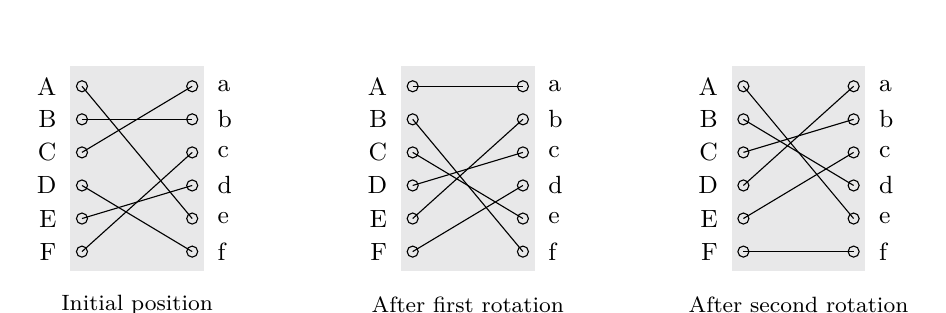
\begin{tikzpicture}[x=1cm,y=-0.42cm,font=\small]
\foreach \panel/\dx/\wires/\name in {0/0/{0/4,1/1,2/0,3/5,4/3,5/2}/Initial position, 1/4.2/{0/0,1/5,2/4,3/2,4/1,5/3}/After first rotation, 2/8.4/{0/4,1/3,2/1,3/0,4/2,5/5}/After second rotation}{
  \fill[gray!20] (\dx+0.25,-0.6) rectangle (\dx+1.95,5.6);
  \foreach \L [count=\i from 0] in {A,B,C,D,E,F}{\node[anchor=east] at (\dx+0.2,\i) {\L}; \draw (\dx+0.4,\i) circle (2pt);}
  \foreach \L [count=\i from 0] in {a,b,c,d,e,f}{\node[anchor=west] at (\dx+2.0,\i) {\L}; \draw (\dx+1.8,\i) circle (2pt);}
  \foreach \l/\r in \wires {\draw (\dx+0.4,\l) -- (\dx+1.8,\r);}
  \node[font=\footnotesize] at (\dx+1.1,6.6) {\name};
}
\end{tikzpicture}
\end{center}
\textbf{Example} (the slide's 6-letter rotor; plaintext on the right, ciphertext on the left). In the initial position \ttx{b} is wired to \ttx{B} and \ttx{e} to \ttx{A}; after the first rotation \ttx{e} is wired to \ttx{C}; after the second, \ttx{e} is wired to \ttx{A} again. If the rotor were stationary (a monoalphabetic substitution), ``bee'' would be encrypted as \ttx{BAA}. With the rotor turning after each letter it becomes \ttx{BCA}: the two \ttx{e}'s are encrypted as different characters. A single rotor of 26 contacts repeats its sequence of permutations every 26 letters, which is still a short period.

\textbf{The Enigma machine} was invented by Arthur Scherbius in 1918 for businesses that needed to send confidential documents without codebooks; it was modified by the German army and used extensively in World War II. It is based on the principle of rotor ciphers, with three rotors connected so that the \textbf{wiring changes as you type}. Its main parts are:
\begin{itemize}[leftmargin=1.4em]
  \item a \textbf{keyboard} for typing the plaintext and a \textbf{lampboard} on which the ciphertext letter lights up;
  \item a \textbf{plugboard} that swaps chosen pairs of letters on the way in and again on the way out;
  \item three \textbf{rotors}: the \emph{fast} rotor turns one position with every key press, the \emph{middle} rotor turns once per revolution of the fast rotor, and the \emph{slow} rotor once per revolution of the middle one (like the wheels of an odometer), so the sequence of substitutions repeats only after about $26^3 = 17\,576$ letters;
  \item a \textbf{reflector}, which sends the current back through the three rotors by a different path.
\end{itemize}
\begin{center}
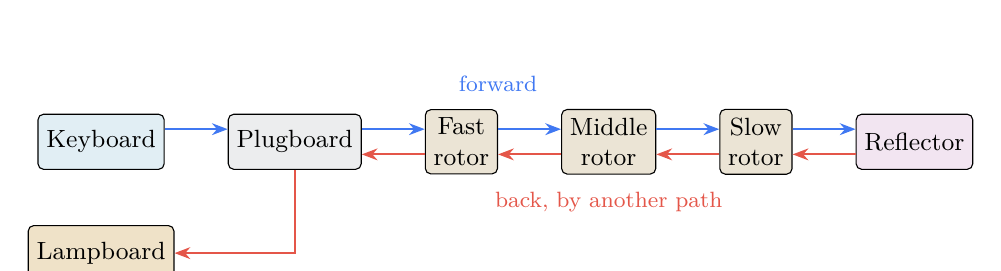
\begin{tikzpicture}[node distance=8mm]
  \node[box,fill=cyan!10] (kb) {Keyboard};
  \node[box,fill=gray!15,right=of kb] (pb) {Plugboard};
  \node[box,fill=orange!15,right=of pb] (f) {Fast\\rotor};
  \node[box,fill=orange!15,right=of f] (m) {Middle\\rotor};
  \node[box,fill=orange!15,right=of m] (s) {Slow\\rotor};
  \node[box,fill=magenta!10,right=of s] (r) {Reflector};
  \node[box,fill=yellow!20,below=7mm of kb] (lb) {Lampboard};
  \foreach \a/\b in {kb/pb,pb/f,f/m,m/s,s/r}{\draw[arr,acc] ([yshift=1.6mm]\a.east) -- ([yshift=1.6mm]\b.west);}
  \foreach \a/\b in {r/s,s/m,m/f,f/pb}{\draw[arr,warn] ([yshift=-1.6mm]\a.west) -- ([yshift=-1.6mm]\b.east);}
  \draw[arr,warn] (pb.south) |- (lb.east);
  \node[font=\footnotesize,acc,above=1mm of f.north east] {forward};
  \node[font=\footnotesize,warn,below=1mm of m.south] {back, by another path};
\end{tikzpicture}
\end{center}
In the slide's example the key \ttx{T} is pressed: the plugboard turns it into \ttx{K}, the three wheels carry it to the reflector, which returns it on another contact, the wheels carry it back to \ttx{W}, and the plugboard turns \ttx{W} into \ttx{G}, so lamp \ttx{G} lights.

\textbf{Consequences of the reflector.} The current path is reversible, so with the same settings pressing \ttx{G} lights \ttx{T}: encryption and decryption are the same operation, which made the machine convenient. But the reflector never connects a contact to itself, so the return path always ends on a different letter: \textbf{Enigma never encrypts a letter to itself}. This was a real weakness. Allied cryptanalysts used it to place a guessed plaintext word (a \emph{crib}) against the ciphertext, rejecting every position where some letter would have mapped to itself, and then searched the rotor settings with machines (the \emph{bombes}). The key of a day was the choice and order of the rotors, their ring settings and starting positions, and the plugboard pairs.

\subsection{Transposition: keyless, keyed, combined \hot}
\asked{Mid-sem 2024--25 Q3(b): ``abcdefghij'' $\to$ ``CABDEHFGIJ'' with a keyed transposition: the pattern repeats every 5 letters, so the permutation key has size \textbf{5}.}
A transposition cipher does not substitute one symbol for another; it changes the location of the symbols (\S\ref{sec:transp}). Forouzan sorts transposition ciphers by how the permutation is produced.

\textbf{Keyless transposition.} Simple transposition ciphers used in the past are keyless: the permutation comes from the shape of a table, not from a key. There are two methods. In the first, the text is written into a table \emph{column by column} and transmitted \emph{row by row}; the rail fence is this method with a 2-row table. To send ``meet me at the park'', Alice writes the letters in a zig-zag over two lines and sends the first line followed by the second: \textbf{\ttx{MEMATEAKETETHPR}}. Bob divides the ciphertext in half (here the second half, \ttx{ETETHPR}, has one character fewer than the first, \ttx{MEMATEAK}), uses the halves as the two rows and reads in zig-zag. In the second method, the text is written \emph{row by row} and transmitted \emph{column by column}. With an agreed 4 columns Alice writes \ttx{meet|meat|thep|ark} and sends \textbf{\ttx{MMTAEEHREAEKTTP}}; Bob writes the ciphertext column by column and reads it row by row.

The permutation of the second method has a visible pattern. Writing each plaintext position under the ciphertext position it moves to,
\begin{center}\small\setlength{\tabcolsep}{3.5pt}
\begin{tabular}{@{}l*{15}{c}@{}}
\toprule
Plaintext position & 01&02&03&04&05&06&07&08&09&10&11&12&13&14&15\\
Ciphertext position & 01&05&09&13&02&06&10&14&03&07&11&15&04&08&12\\
\bottomrule
\end{tabular}
\end{center}
the second character has moved to the fifth position, the third to the ninth, and so on. The permutation falls into runs $(01, 05, 09, 13)$, $(02, 06, 10, 14)$, $(03, 07, 11, 15)$, $(04, 08, 12)$, in each of which adjacent numbers differ by 4, the number of rows. Such regularity is what the pattern attack below exploits.

\textbf{Keyed (block) transposition.} Instead of permuting the whole text at once, the plaintext is divided into groups of a predetermined size, called \textbf{blocks}, and the characters of each block are permuted separately with a \textbf{permutation key}. Alice and Bob agree to send ``Enemy attacks tonight'' in blocks of five, adding a bogus character \ttx{z} to fill the last block: \ttx{enemy attac kston ightz}. With the encryption key \textbf{(3 1 4 5 2)}, \emph{position $i$ of the ciphertext block takes the character at position key[$i$] of the plaintext block}: the third character becomes the first, the first becomes the second, the fourth the third, and so on. So \ttx{enemy} $\to$ \ttx{EEMYN}, and the ciphertext is \textbf{\ttx{EEMYN TAACT TKONS HITZG}}. Bob divides the ciphertext into 5-character groups and applies the key in the reverse direction. Since letters are only moved, changing one plaintext letter changes exactly one ciphertext letter.

\textbf{The past-paper question.} Eve types ``abcdefghij'' on Alice's computer and sees ``CABDEHFGIJ''. This is a \textbf{chosen-plaintext attack}, and the choice of plaintext is clever: all letters are different, so each output letter reveals its source position directly. \ttx{abcde} $\to$ \ttx{CABDE} and \ttx{fghij} $\to$ \ttx{HFGIJ} both take input positions 3, 1, 2, 4, 5, so the pattern repeats every 5 letters: the key has size \textbf{5}, the encryption key is \textbf{(3 1 2 4 5)}, and the decryption key is its inverse \textbf{(2 3 1 4 5)}.

\textbf{Combining the two approaches (keyed columnar transposition).} More recent transposition ciphers combine the two approaches to achieve better scrambling. Encryption is done in three steps: the text is \textbf{written into a table row by row}, the \textbf{columns are permuted} with the key, and the new table is \textbf{read column by column}. The first and third steps give a keyless \emph{global} reordering, and the second a \emph{blockwise keyed} reordering (each row is a block). Such ciphers are called \textbf{keyed columnar} or simply \textbf{columnar transposition ciphers}. With the key (3 1 4 5 2):
\begin{center}\small
\begin{tabular}{@{}c@{\quad}c@{\quad}c@{}}
Written row by row & Columns permuted (3 1 4 5 2) & Read column by column\\[2pt]
\begin{tabular}{|ccccc|}\hline e&n&e&m&y\\ a&t&t&a&c\\ k&s&t&o&n\\ i&g&h&t&z\\\hline\end{tabular}
&
\begin{tabular}{|ccccc|}\hline E&E&M&Y&N\\ T&A&A&C&T\\ T&K&O&N&S\\ H&I&T&Z&G\\\hline\end{tabular}
&
\ttx{ETTH EAKI MAOT YCNZ NTSG}
\end{tabular}
\end{center}
Ciphertext \textbf{\ttx{ETTHEAKIMAOTYCNZNTSG}}. Bob reverses the steps: he writes the ciphertext column by column, permutes the columns with the decryption key, and reads row by row.

\begin{trap}[: two ways to write a column key]
The Neso row--column key (\S\ref{sec:transp}) writes above each column its \emph{rank in the reading order} (4 3 1 2 5 6 7 means column 3 is read first). Forouzan's key lists, for each output position, the \emph{source column} (3 1 4 5 2 means column 3 goes first). The two notations are inverse permutations of each other: the Neso key 4 3 1 2 5 6 7 is Forouzan's (3 4 2 1 5 6 7). State which convention you use.
\end{trap}

\subsection{Encryption and decryption keys of a transposition}
A single key is used in two directions for the column exchange: downward for encryption and upward for decryption. It is customary to create two keys from it, one for encryption and one for decryption, each stored as a table with one entry per column. \textbf{Each entry shows the source column number; the destination column number is understood from the position of the entry.} The encryption key (3 1 4 5 2) says that column 3 of the source becomes column 1 of the destination; the decryption key (2 5 1 3 4) says that column 2 of the source becomes column 1 of the destination.

\textbf{Inverting a key.} Encryption sends source column $e_i$ to destination $i$. Decryption must send it back: the column now at position $i$ must return to position $e_i$, i.e.\ the decryption key has the entry $i$ at position $e_i$. Hence the algorithm on the slide:
\begin{center}\small\ttfamily
\begin{tabular}{@{}l@{}}
for index = 1 to Column:\quad DecKey[EncKey[index]] $\leftarrow$ index
\end{tabular}
\end{center}
By hand: write the index $1, 2, \dots$ under the encryption key, swap the two rows, and sort the pairs by the (former) key row; the index row becomes the decryption key. For the slide's key (2 6 3 1 4 7 5):
\begin{center}\small
\begin{tabular}{@{}l*{7}{c}@{\qquad}l*{7}{c}@{}}
\toprule
Encryption key & 2&6&3&1&4&7&5 & Sorted by key & 1&2&3&4&5&6&7\\
Index & 1&2&3&4&5&6&7 & Index $=$ decryption key & \textbf{4}&\textbf{1}&\textbf{3}&\textbf{5}&\textbf{7}&\textbf{2}&\textbf{6}\\
\bottomrule
\end{tabular}
\end{center}
Check: key value 1 stood at index 4, so DecKey[1] $= 4$; key value 2 stood at index 1, so DecKey[2] $= 1$. Likewise (3 1 4 5 2) inverts to (2 5 1 3 4).

\textbf{Transposition as a matrix.} The plaintext and ciphertext blocks can be written as $1 \times m$ row vectors of letter values and the key as an $m \times m$ \textbf{permutation matrix}, in which every row and every column has exactly one 1 and the rest are 0s. Column $j$ of the key has its 1 in row key[$j$], so multiplying a block by it copies input position key[$j$] to output position $j$. Encryption is $C = PK$ and decryption $P = CK^{-1}$, as in the Hill cipher; a transposition is a Hill cipher whose matrix only moves letters. The inverse needs no computation: $K^{-1} = K^{T}$. Indeed $(KK^T)_{ij} = \sum_l K_{il}K_{jl}$; for $i = j$ the single 1 of row $i$ meets itself and the sum is 1, while for $i \ne j$ the 1s of rows $i$ and $j$ lie in different columns (each column has only one 1) and the sum is 0. With the key (3 1 4 5 2) and the four blocks of ``enemyattackstonightz'' as rows:
\[
\small
\begin{pmatrix}04&13&04&12&24\\00&19&19&00&02\\10&18&19&14&13\\08&06&07&19&25\end{pmatrix}
\begin{pmatrix}0&1&0&0&0\\0&0&0&0&1\\1&0&0&0&0\\0&0&1&0&0\\0&0&0&1&0\end{pmatrix}
=
\begin{pmatrix}04&04&12&24&13\\19&00&00&02&19\\19&10&14&13&18\\07&08&19&25&06\end{pmatrix}
\]
that is \ttx{EEMYN TAACT TKONS HITZG}, the keyed block transposition above; multiplying by $K^T$ returns \ttx{enemy attac kston ightz}.

\subsection{Cryptanalysis of transposition ciphers}
Transposition ciphers are vulnerable to several kinds of ciphertext-only attack.

\textbf{Statistical attack.} Single-letter frequency analysis does not reveal the key, but since the letters are unchanged it immediately shows that the cipher is a transposition (and what language the plaintext is in); digram and trigram statistics then guide the reordering.

\textbf{Brute-force attack.} Eve can try all possible keys, but if the key length is unknown their number is huge, $1! + 2! + 3! + \dots + L!$ for an $L$-letter ciphertext. A better approach is to guess the number of columns. If the table is full, the number of columns divides $L$: for $L = 20 = 2 \times 2 \times 5$ it is one of $1, 2, 4, 5, 10, 20$, where 1 column (no change) is out of the question and 20 (a single row) is unlikely. For each candidate $c$ only $c!$ orders remain ($5! = 120$ for $c = 5$).

\textbf{Pattern attack.} The ciphertext of a keyed (columnar) transposition has repeated patterns. For the ciphertext \ttx{ETTHEAKIMAOTYCNZNTSG} above, the plaintext positions of the ciphertext letters are
\begin{center}\small\ttfamily
03 08 13 18 \;01 06 11 16 \;04 09 14 19 \;05 10 15 20 \;02 07 12 17
\end{center}
The first ciphertext character comes from the third plaintext character, and within each group of four adjacent numbers differ by 5, the number of columns. If Eve knows or guesses that there are 5 columns, she organises the ciphertext in groups of four characters (each group is one column of the table), and permuting the groups ($5! = 120$ orders at most, far fewer with digram clues) reveals the plaintext.

\textbf{Double transposition.} Double transposition ciphers make the cryptanalyst's job much harder. The whole algorithm is applied twice, normally with the same key (a different key can be used in each step). Encrypting the middle text \ttx{ETTHEAKIMAOTYCNZNTSG} again with (3 1 4 5 2) gives the ciphertext \textbf{\ttx{TIYTEAOZHMCSEANGTKTN}}, whose plaintext positions are
\begin{center}\small\ttfamily
13 16 05 07 03 06 14 20 18 04 10 12 01 09 15 17 08 11 19 02
\end{center}
No constant difference survives, so grouping the ciphertext by columns no longer gives pieces of plaintext rows. The single-letter frequency attack still works (the letters are still those of the plaintext), but the pattern attack is now much more difficult. As in \S\ref{sec:transp}, the double transposition is still one permutation of the 20 positions; what it removes is the regular columnar structure that the pattern attack depends on.

\subsection{Stream vs.\ block ciphers}
Symmetric ciphers fall into two broad categories. In a \textbf{stream cipher}, encryption and decryption are done \textbf{one symbol (a character or a bit) at a time}. There is a plaintext stream $P = P_1P_2P_3\dots$, a ciphertext stream $C = C_1C_2C_3\dots$ and a key stream $K = (k_1, k_2, k_3, \dots)$, and
\[
C_1 = E_{k_1}(P_1),\quad C_2 = E_{k_2}(P_2),\quad C_3 = E_{k_3}(P_3),\ \dots
\]
The ciphers differ only in how the key stream is made: the additive cipher repeats one value ($k_i = k$), the monoalphabetic cipher uses one fixed table, Vigen\`ere repeats $m$ values, the autokey takes its values from the plaintext, the rotor cipher uses the sequence of rotor positions, and the one-time pad uses fresh random values.

In a \textbf{block cipher}, a group of plaintext symbols of size $m$ ($m > 1$) is encrypted \textbf{together}, creating a ciphertext group of the same size. A single key is used to encrypt the whole block, even if the key is made of several values, and \textbf{each ciphertext block depends on the whole plaintext block}. Playfair ($m = 2$: the output for a letter depends on its partner) and Hill ($m \times m$ key) are block ciphers, and so are the modern DES and AES (64- and 128-bit blocks, \S\ref{sec:modern}). In practice the two ideas are combined: a block cipher encrypts the blocks of a long message one after another, so at the level of single blocks it is a block cipher, but considering each block as one unit the message is processed as a stream of blocks.

The difference shows in how far one plaintext change spreads, which past papers ask directly:
\begin{center}\small
\begin{tabular}{@{}lcl@{}}
\toprule
Cipher & Ciphertext characters changed & Reason\\
\midrule
Additive, multiplicative, affine & 1 & monoalphabetic, letter by letter\\
Vigen\`ere, one-time pad & 1 & stream: one key value per letter\\
Autokey & 2 & $P_i$ is also the key of a later letter\\
Keyed transposition & 1 & the letter is moved, not changed\\
Playfair & 2 (usually) & the digram is one block\\
Hill with $m \times m$ key & up to $m$ & every output letter uses the whole block\\
\bottomrule
\end{tabular}
\end{center}

\begin{trap}[: Vigen\`ere is a stream cipher]
Even though the key repeats every $m$ letters, Vigen\`ere encrypts one character at a time, each with its own key element: a \textbf{stream} cipher. Playfair works on pairs, Hill on $m$-letter blocks: \textbf{block} ciphers.
\end{trap}

\section{Classical Ciphers at a Glance}
The table collects every classical cipher of the course with its key and the weakness that breaks it. The pattern is consistent: a cipher is broken through whatever structure the key fails to destroy, whether that is a tiny key space, preserved letter or digram frequencies, a period, linearity or a regular position pattern.
\begin{center}\small
\begin{tabularx}{\textwidth}{@{}l l l X@{}}
\toprule
Cipher & Type & Key & Main weakness\\
\midrule
Caesar & substitution, 1 letter & shift 3 (fixed) & algorithm known, no real key\\
Shift & substitution, 1 letter & shift 1--25 & only 25 keys: brute force\\
Multiplicative & substitution, 1 letter & $k \in \mathbb{Z}_{26}^*$ (12) & brute force; frequencies preserved\\
Affine & substitution, 1 letter & $(k_1, k_2)$: 312 keys & two known pairs give the key\\
Monoalphabetic & substitution, 1 letter & permutation ($26!$) & letter frequencies preserved\\
Playfair & substitution, 2 letters & 5$\times$5 keyword matrix & same pair $\to$ same output\\
Hill & substitution, $m$ letters & invertible $m\times m$ matrix & linear (known plaintext)\\
Vigen\`ere & polyalphabetic & repeating keyword & key repeats: Kasiski/IC, then Caesars\\
Autokey & polyalphabetic & keyword + plaintext & key has English frequencies\\
Vernam & polyalphabetic, bits (XOR) & key stream & tape key repeated\\
Rotor, Enigma & polyalphabetic, stream & wiring, rotor positions & finite period; Enigma never maps a letter to itself\\
One-time pad & substitution & random, once, message length & none (perfect secrecy); key generation and distribution\\
Rail fence & transposition & depth & few possibilities\\
Row--column & transposition & column order (+ stages) & one stage can be reconstructed\\
Keyed / columnar & transposition & permutation of $m$ positions & pattern attack (double transposition resists it)\\
\bottomrule
\end{tabularx}
\end{center}
Transposition ciphers keep the letter frequencies of the plaintext unchanged (only positions move); substitution ciphers keep the positions and change the letters.

\begin{fixbox}
\begin{itemize}[leftmargin=1.2em,itemsep=0pt]
  \item Kasiski slide: ``the cryptanalyst assumes that $d \mid m$'' and ``$\gcd(d_1, \dots, d_n)/m$'' should read $m \mid d$ and $m \mid \gcd(d_1, \dots, d_n)$: the key length divides the distances, not the other way round.
  \item Kasiski example: the indices 68/168, 69/117, 72/132, 119/127 count from 0 (from 1 they are 69/169, 70/118, 73/133, 120/128); the differences 100, 48, 60, 8 are unaffected.
  \item Kasiski example: the slide's rows P1--P4 are not the decryptions of C1--C4 from the 21st letter of each piece onward. The ciphertext was made from a copy of the sentence with typos (decrypted with key \ttx{code}, ``shift'' lacks its \ttx{f}, ``shifted'' ends in \ttx{r}, the \ttx{t} of ``to'' is missing and an extra \ttx{a} precedes ``ciphertext''), while P1--P4 were written from the corrected sentence. The key \ttx{code} and the method are right.
  \item Affine attack: ``The square matrix and its inverse are the same'' means they are the same as in the first attempt (both use the plaintext ``et''); $\left(\begin{smallmatrix}4&1\\19&1\end{smallmatrix}\right)$ is not its own inverse, which is $\left(\begin{smallmatrix}19&7\\3&24\end{smallmatrix}\right)$.
  \item Keyless transposition slide: the mapping row shows 13 under plaintext position 8 and the run $(02, 06, 10, 13)$; both should be 14. The runs are $(01,05,09,13)$, $(02,06,10,14)$, $(03,07,11,15)$, $(04,08,12)$.
  \item Double transposition slide: the ciphertext is \ttx{TIYTEAOZHMCSEANG}\textbf{\ttx{T}}\ttx{KTN}, not \ttx{\dots EANGYKTN}; in the position list the seventh entry is \textbf{14}, not a second 10.
  \item ``Keys'' slide: ``one for encryption and one for direction'' should be ``one for decryption''. Enigma slide: the inventor is Arthur \emph{Scherbius}.
  \item Stream/block slide lists ``Polyalphabetic cipher'' under block ciphers while listing Vigen\`ere under stream ciphers. By the slide's own definitions, polyalphabetic ciphers that encrypt one letter at a time (Vigen\`ere, autokey, rotor) are stream ciphers.
\end{itemize}
\end{fixbox}

% Sources: Neso videos (steganography, LSB steganography demo, abstract algebra & number theory intro, prime numbers;
% notes6.md), Stallings 2.5 (steganography). Numbers checked by script (scratchpad/r3/verify3.py).
\definecolor{puregreen}{RGB}{0,255,0}
\definecolor{modgreen}{RGB}{0,252,0}

\section{Steganography}\label{sec:stego}
Encryption hides the \emph{meaning} of a message but not the fact that a secret message is being sent. Ciphertext looks like random gibberish, so it draws attention: an observer immediately knows that something is worth intercepting, may block it, or may pressure the sender and receiver for the key. \textbf{Steganography} (Greek ``covered writing'') solves a different problem. It \textbf{conceals the existence of the message} by hiding it inside an innocent-looking \textbf{cover} such as a text, an image or an audio file, so that an observer does not suspect that any secret communication is taking place. It is \textbf{not an encryption scheme}: the message is not transformed into something unintelligible but merely hidden, and its protection lies in going unnoticed. \textbf{Cryptography}, by contrast, renders the message unintelligible to outsiders by various transformations of the text.

\imp{Cryptography hides the meaning of a message; steganography hides its existence.}
\begin{center}\small
\begin{tabularx}{\textwidth}{@{}l X X@{}}
\toprule
 & \textbf{Cryptography} & \textbf{Steganography}\\
\midrule
Hides & the \textbf{meaning} & the \textbf{existence}\\
Attacker sees & a scrambled message; knows something secret is being sent & an ordinary-looking text/image; doesn't suspect anything\\
Output & ciphertext & a normal-looking \textbf{cover} (text, image, audio) with the message inside\\
\bottomrule
\end{tabularx}
\end{center}
Steganography is the other kind of ``security-related transformation'' $T$ in the model for network security (\S\ref{sec:netmodel}): the transformation applied to the message before transmission does not have to be encryption.

\textbf{Examples from the lecture.} The simplest text steganography arranges words so that some of their letters spell the real message, here the first letter of each word (an \emph{acrostic}, or null cipher). The cover sentence reads as ordinary if odd text, and the secret is the rule ``read the first letters'':
\begin{itemize}
  \item \textbf{S}imply \textbf{e}ncrypt \textbf{c}orrect \textbf{r}eading \textbf{e}xactly \textbf{t}wice. $\Rightarrow$ \textbf{Secret}
  \item \textbf{T}ell \textbf{h}enry \textbf{a}lice \textbf{n}ot \textbf{k}ane / \textbf{Y}esterday \textbf{o}urplan \textbf{u}ndone! $\Rightarrow$ \textbf{Thank You}
\end{itemize}

\subsection{Historical techniques}
Before computers, messages were hidden physically in ordinary documents. Stallings lists four classical techniques; each leaves the document readable as normal text and reveals the hidden marks only under a special treatment that an inspector would not think of applying.
\begin{center}\small
\begin{tabularx}{\textwidth}{@{}l X@{}}
\toprule
Character marking & Chosen letters of a printed or typewritten text are overwritten faintly in pencil. The marks are not visible unless the paper is held at an angle to bright light.\\
Invisible ink & Written with a substance (e.g.\ lemon juice) that leaves no visible trace until heat or a chemical is applied.\\
Pin punctures & Tiny pin holes on selected letters. They are not visible unless the paper is held up in front of a light.\\
Typewriter correction ribbon & Text typed between the lines with a correction ribbon. It is visible only under a strong light.\\
\bottomrule
\end{tabularx}
\end{center}
Modern steganography hides data in digital media instead. Stallings' example is a high-resolution photograph (Kodak Photo CD, $2048 \times 3072$ pixels of 24 bits): changing only the least significant bit of each colour byte does not visibly affect the picture, yet hides $2048 \times 3072 \times 3 = 18\,874\,368$ bits, about 2.3 MB, in a single snapshot. This LSB method is explained below.

\subsection{Drawbacks}
Compared with encryption, steganography has two drawbacks.
\begin{enumerate}[leftmargin=1.5em]
  \item \textbf{Lots of overhead.} A large cover is needed to hide relatively few bits of message: a whole sentence for six letters in the acrostic above, a whole image for a few kilobytes.
  \item \textbf{Once the system is discovered, it becomes virtually worthless.} The security rests entirely on the method staying unknown, which contradicts Kerckhoff's principle (\S\ref{sec:attacks}). Unlike encryption, there is no secret key left to protect the message once the method is known. This can be softened by making the insertion depend on a key (for example, a key that selects which pixels carry the bits).
\end{enumerate}
\textbf{Advantage.} Steganography can be used by parties who have something to lose if the \emph{fact} of their secret communication (not necessarily its content) is discovered. Encryption flags the traffic as important or secret, and may mark the sender or receiver as someone with something to hide; a stego image is just a photograph.

\textbf{Best of both.} A message can be \textbf{first encrypted and then hidden} using steganography. The hiding conceals that communication is taking place, and if the hiding is discovered the attacker still only has ciphertext, which is protected by the key. Encrypted data also looks random, like the noise in the least significant bits it replaces, which makes the hidden data harder to detect statistically.
\begin{center}
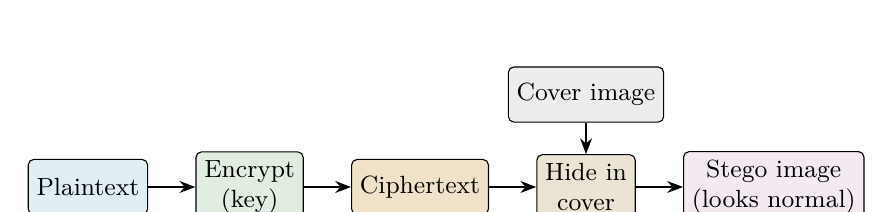
\begin{tikzpicture}[node distance=6mm]
  \node[box,fill=cyan!10] (p) {Plaintext};
  \node[box,fill=green!15,right=of p] (e) {Encrypt\\(key)};
  \node[box,fill=yellow!20,right=of e] (c) {Ciphertext};
  \node[box,fill=orange!15,right=of c] (h) {Hide in\\cover};
  \node[box,fill=gray!15,above=4mm of h] (cv) {Cover image};
  \node[box,fill=magenta!8,right=of h] (s) {Stego image\\(looks normal)};
  \draw[arr] (p)--(e); \draw[arr] (e)--(c); \draw[arr] (c)--(h); \draw[arr] (cv)--(h); \draw[arr] (h)--(s);
\end{tikzpicture}
\end{center}

\subsection{LSB steganography}
A byte $b_7 b_6 \dots b_1 b_0$ has the value $128 b_7 + 64 b_6 + \dots + 2 b_1 + b_0$. The leftmost bits are the \textbf{most significant bits} (MSB), because changing them changes the value a lot; the rightmost bits are the \textbf{least significant bits} (LSB), which change it the least:
\[
1010\,10\underbrace{01}_{\text{LSBs}} \qquad\text{bit weights: } 128\;64\;32\;16\;8\;4\;\underline{2\;1}
\]
Changing the lowest $k$ bits of a byte changes its value by at most $2^k - 1$. For $k = 2$ that is at most 3 out of 255, about 1.2\% of the range, which the eye cannot see in a colour.

\textbf{RGB model.} In a 24-bit colour image each pixel is stored as three bytes, one each for the intensity of \textbf{Red}, \textbf{Green} and \textbf{Blue} (0--255).
\begin{center}\small Red $(255,0,0) = (\ttx{11111111}, \ttx{00000000}, \ttx{00000000})$ \quad Green $(0,255,0)$ \quad Blue $(0,0,255)$\end{center}

\begin{center}
\begin{tikzpicture}
  \fill[puregreen] (0,0) rectangle (3.2,1.4);
  \fill[modgreen] (4.2,0) rectangle (7.4,1.4);
  \node[font=\small,below] at (1.6,0) {$(0, 255, 0)$, G $=$ \ttx{111111\textbf{11}}};
  \node[font=\small,below] at (5.8,0) {$(0, 252, 0)$, G $=$ \ttx{111111\textbf{00}}};
\end{tikzpicture}
\end{center}
The two boxes look identical, but the last 2 bits of their green values differ. \textbf{Those LSBs can therefore store hidden information}: the sender overwrites them with message bits, and the image looks unchanged. Using the 2 LSBs of each of R, G and B hides $2 \times 3 = \mathbf{6}$ \textbf{bits per pixel}, and no channel value changes by more than 3. To extract the message the receiver simply reads the last 2 bits of each channel, in the agreed order of pixels, and concatenates them.

\begin{worked}[: hiding bits in one pixel]
\textbf{Q.} Hide the six bits \ttx{11 01 10} in the pixel $(100, 50, 200)$ using the 2 LSBs of each channel. By how much does each value change?

Write each value in binary and replace its last two bits with the next two message bits:
\begin{center}\small
\begin{tabular}{@{}lllll@{}}
\toprule
Channel & Value & Binary & Replace last 2 bits & New value\\
\midrule
R & 100 & \ttx{011001\textbf{00}} & \ttx{011001\textbf{11}} & 103 ($+3$)\\
G & 50 & \ttx{001100\textbf{10}} & \ttx{001100\textbf{01}} & 49 ($-1$)\\
B & 200 & \ttx{110010\textbf{00}} & \ttx{110010\textbf{10}} & 202 ($+2$)\\
\bottomrule
\end{tabular}
\end{center}
New pixel \textbf{(103, 49, 202)}; every channel changes by at most 3, as predicted. Check: the last two bits of 103, 49, 202 are \ttx{11}, \ttx{01}, \ttx{10} \checkmark.
\end{worked}

\textbf{Capacity.} With 6 bits per pixel an $800 \times 600$ image holds $800 \cdot 600 \cdot 6 = 2{,}880{,}000$ bits $= 360{,}000$ bytes. With only the single LSB of each channel (3 bits per pixel) a $1024 \times 768$ image holds $1024 \cdot 768 \cdot 3 = 2{,}359{,}296$ bits $= 294{,}912$ bytes. The lecture's 17-byte message ``Kill Corona Virus'' is $17 \times 8 = 136$ bits, which needs only $\lceil 136 / 6 \rceil = 23$ pixels at 6 bits per pixel.

\textbf{Blue orchids:} the lecture shows the image without and with hidden information side by side, and they cannot be told apart.

\textbf{Detection.} Looking at the image reveals nothing, but a statistical analysis may. In a natural photograph the LSBs are correlated with the rest of the image, while embedded data (especially encrypted data) is uniformly random, so the LSB plane of a stego image has slightly different statistics; a changed file format or file size is a further clue (see the OpenStego demo below). The study of detecting hidden data is called \textbf{steganalysis}.

\subsection{Watermarking vs.\ image steganography}
Both techniques embed extra information in an image, but for opposite purposes. A \textbf{watermark} is embedded to \textbf{prove ownership} or copyright: the logo or owner information is not secret, it is often visible (like the \ttx{nesoacademy.org} mark on the lecture's laptop image), and it must survive cropping and compression so that it can still be shown later. \textbf{Image steganography} embeds a message for \textbf{secret communication}: its \textbf{existence} must stay hidden, and robustness matters less than going unnoticed.
\begin{center}\small
\begin{tabularx}{\textwidth}{@{}l X X@{}}
\toprule
 & \textbf{Watermarking} & \textbf{Image steganography}\\
\midrule
Purpose & prove \textbf{ownership} / copyright & \textbf{secret communication}\\
Is the mark secret? & no; it's often visible (like the \ttx{nesoacademy.org} logo) & yes; its \textbf{existence} is hidden\\
Hidden data & logo, owner info & any message or file\\
\bottomrule
\end{tabularx}
\end{center}

\subsection{OpenStego demo}
OpenStego is a free tool that embeds a file in an image and extracts it again. The lecture uses it in both directions:
\begin{enumerate}[leftmargin=1.5em]
  \item \textbf{Hide Data:} message file \ttx{My Message.txt} (``Kill Corona Virus'', 17 bytes) + cover file \ttx{Blue Orchids.jpg} (58.4 KB) $\to$ stego file \ttx{BO.png} (824 KB). No password. ``Message embedded into 1 cover file(s).''
  \item \textbf{Extract Data:} input \ttx{BO.png} $\to$ output folder. ``Message file extracted successfully'', and the text file comes back unchanged.
\end{enumerate}
\textbf{Why PNG, and why so much bigger} (not explained in the video): JPEG compression is lossy, so it slightly changes pixel values when the image is saved, which would wipe out the hidden LSBs. The stego image is therefore saved in the lossless PNG format, which stores every pixel exactly and is much larger (58.4 KB $\to$ 824 KB). That size jump is itself a hint that something is going on. Leaving the password empty means the extraction needs no key, so anyone who suspects the file and has the tool can read the message; with a password OpenStego encrypts the data before hiding it, which is the encrypt-then-hide combination above.

\section{Prime Numbers}\label{sec:primesintro}
\textbf{Why the course turns to mathematics.} Classical ciphers substitute and move letters. Modern cryptography treats plaintext and ciphertext as \emph{numbers}, and most encryption is based heavily on \textbf{number theory} and \textbf{abstract algebra}; calculus and trigonometry make no major contribution. The concepts needed are the division and Euclidean algorithms and the extended Euclidean algorithm (\S\ref{sec:exteuclid}), modular arithmetic (\S\ref{sec:modular}), groups, rings, fields and finite fields with polynomial arithmetic (\S\ref{sec:algebra}), Euler's totient (\S\ref{sec:totient}), Fermat's and Euler's theorems (\S\ref{sec:fermat}), and primality testing, the Chinese remainder theorem and discrete logarithms (\S\ref{sec:primes}). The lecture also notes that this is cryptography for classical computers; quantum computers will need different assumptions, because a quantum algorithm (Shor's) factors efficiently. Primes come first because almost everything else is built on them.

\textbf{Definitions.} A \textbf{prime} is an integer greater than 1 with exactly two divisors, 1 and itself: it cannot be divided by any other number without leaving a remainder. A \textbf{composite} number has more than two divisors. \textbf{1 is neither}, because it has only one divisor. Examples: 2, 3, 5, 7 are prime; $9 = 3^2$ (divisors 1, 3, 9) and $33 = 3 \cdot 11$ (divisors 1, 3, 11, 33) are composite.

\textbf{Facts.} 2 is the smallest prime and the \textbf{only even prime}, since every larger even number has 2 as a third divisor. Except for 2 and 5, every prime ends in the digit 1, 3, 7 or 9: a number ending in 0, 2, 4, 6 or 8 is divisible by 2, and one ending in 5 is divisible by 5. (The converse fails: $33$ and $39$ end in 3 and 9 but are composite.)

\textbf{Every number has prime factors.} By the \textbf{fundamental theorem of arithmetic}, every integer $n > 1$ can be written as a product of primes in exactly one way, apart from the order of the factors. A prime is its own factorisation; 1 is not a factor to be listed, since it is not prime.
\begin{center}\small
\begin{tabular}{@{}rl@{\qquad}rl@{}}
\toprule
$n$ & factorisation & $n$ & factorisation\\
\midrule
10 & $2 \cdot 5$ & 37 & $37$ (prime)\\
11 & $11$ (prime) & 308 & $2^2 \cdot 7 \cdot 11$\\
100 & $2^2 \cdot 5^2$ (9 divisors) & 14688 & $2^5 \cdot 3^3 \cdot 17$\\
\bottomrule
\end{tabular}
\end{center}
The number of divisors follows from the factorisation: a divisor of $2^2 \cdot 5^2$ is $2^a 5^b$ with $a, b \in \{0, 1, 2\}$, giving $3 \times 3 = 9$ divisors of 100 (1, 2, 4, 5, 10, 20, 25, 50, 100).

\subsection{Why primes matter in cryptography}
Many encryption algorithms, RSA first among them (\S\ref{sec:rsa}), are based on prime numbers, because of an asymmetry in the work involved. \textbf{Multiplying} two large primes is \textbf{very fast}: two 300-digit numbers are multiplied in a fraction of a millisecond. The \textbf{reverse}, \textbf{factoring} the product back into its primes, is \textbf{extremely computer-intensive}: no known classical algorithm does it in polynomial time, and for a product of two well-chosen 1024-bit primes all the computers in the world would take far too long (\S\ref{sec:primes} covers the factoring methods).
\[
p, q \;\xrightarrow{\text{easy}}\; n = p \cdot q \qquad\qquad n \;\xrightarrow{\text{very hard}}\; p, q
\]
A function that is easy to compute but infeasible to reverse is called a \textbf{one-way function}; if a secret (here the primes $p$ and $q$) makes the reverse easy, it is a \textbf{trapdoor one-way function}, which is exactly what a public-key cipher needs. Cryptographic algorithms therefore use \textbf{large} primes, hundreds of digits long. The lecture closes with six numbers to test, from 4 to 34 digits: 5393, 27644437, 4398042316799, 1125899839733759, 18014398241046527 and 1298074214633706835075030044377087. \textbf{All six are prime} (checked with the Miller--Rabin test of \S\ref{sec:primes}); trial division would need about $\sqrt{n}$ steps, which is hopeless for the last one, and this is why fast probabilistic primality tests matter.

\begin{mustknow}[: primes]
Prime: $> 1$ with exactly two divisors (1 and itself); 1 is not prime; 2 is the only even prime. Every $n > 1$ factors uniquely into primes, e.g.\ $14688 = 2^5 \cdot 3^3 \cdot 17$.\\
Security of RSA-type systems rests on \textbf{factoring the product} $n = pq$ of two large primes being infeasible, while multiplying $p$ and $q$ is easy.
\end{mustknow}

\begin{fixbox}
\begin{itemize}
  \item \textbf{Slide wording:} ``Factoring very large prime numbers is very hard'' should say factoring the \emph{product} of two large primes. A prime can't be factored at all.
  \item The factorisation table writes $11 = 1^1 \times 11^1$ and lists 1 as a prime factor. 1 is not prime; 11 and 37 are simply prime.
  \item The notes call watermarks ``typically visible''. The lecture's example is visible, but watermarks can also be invisible. The real difference is the purpose (ownership vs.\ secret communication).
  \item Fermat's and Euler's theorems need $\gcd(a,p) = 1$ / $\gcd(a,n) = 1$; the notes omitted this condition.
  \item Everything else checked: TOMATO $\to$ (a) (by script), $N(N-1)/2$, all six numbers prime, factorisations correct.
\end{itemize}
\end{fixbox}


\part{Mathematics of Cryptography}
% College Lecture 2 (integer division) + Lecture 4 (modular arithmetic, inverses, Z_n, Z_n^*), Neso videos on modular
% arithmetic (notes7.md), Forouzan ch. 2 (2.1, 2.2, 2.4 linear congruences). Every number recomputed by script (scratchpad/r4/verify.py).
\section{Modular Arithmetic}\label{sec:modular}

Modular arithmetic is integer arithmetic in which only the remainder after division by a fixed positive integer $n$ is kept, so that counting wraps around to 0 after reaching $n - 1$. Cryptography needs it for two reasons. First, a cipher must map a finite alphabet onto itself: shifting Y by 3 has to land on a letter again, which is achieved by wrapping around after 25. Second, public-key systems compute with numbers that are hundreds of digits long, and modular arithmetic keeps every intermediate result below the modulus however many operations are performed. This section builds the arithmetic from the division algorithm and ends with the two questions that recur in every later chapter: when can we divide modulo $n$, and how do we solve $ax \equiv b \pmod n$.

\subsection{Integer division and residues}
The set of integers $\mathbb{Z} = \{\dots, -2, -1, 0, 1, 2, \dots\}$ is closed under the three binary operations cryptography uses (addition, subtraction and multiplication) but not under division, since $7/2$ is not an integer. Integer division therefore has two outputs instead of one. \imp{For any integer $a$ and any positive integer $n$ there are unique integers $q$ (the quotient) and $r$ (the remainder) with $a = q \times n + r$ and $0 \le r < n$.} This statement is the \textbf{division algorithm}. For $a = 255$ and $n = 11$ it gives $255 = 23 \times 11 + 2$, so $q = 23$ and $r = 2$.

The pair $(q, r)$ is unique because of the condition $0 \le r < n$: if $a = qn + r = q'n + r'$, then $r - r' = (q' - q)n$ is a multiple of $n$ lying strictly between $-n$ and $n$, so it is 0. Geometrically, $qn$ is the largest multiple of $n$ that does not exceed $a$, and $r$ is the distance from that multiple up to $a$. The picture settles the case of a negative $a$ as well: the largest multiple of $n$ not exceeding $a$ then lies to the \emph{left} of $a$, further from zero, so $r$ is still non-negative.
\begin{center}
\begin{tikzpicture}[x=10mm,y=1mm,font=\footnotesize]
  % positive a
  \draw[-{Stealth[length=2mm]}] (-0.4,0) -- (8.7,0);
  \foreach \x/\l in {0/0,1.2/11,2.4/22,6/253,8.2/264}{\draw (\x,1.5) -- (\x,-1.5) node[below]{\l};}
  \node at (4.2,-4) {$\cdots$};
  \fill[acc] (6.4,0) circle (0.6mm) node[above=0.5mm,acc]{$a = 255$};
  \draw[{Stealth[length=1.2mm]}-{Stealth[length=1.2mm]},good,thick] (6,-9) -- node[below]{$r = 2$} (6.4,-9);
  \node[anchor=west,gray] at (8.9,0) {$a \ge 0$: $255 = 23 \times 11 + 2$};
  % negative a
  \begin{scope}[yshift=-27mm]
  \draw[-{Stealth[length=2mm]}] (-0.4,0) -- (8.7,0);
  \foreach \x/\l in {0/$-264$,2.2/$-253$,5.8/$-22$,7/$-11$,8.2/0}{\draw (\x,1.5) -- (\x,-1.5) node[below]{\l};}
  \node at (4,-4) {$\cdots$};
  \fill[acc] (1.8,0) circle (0.6mm) node[above=0.5mm,acc]{$a = -255$};
  \draw[{Stealth[length=1.2mm]}-{Stealth[length=1.2mm]},good,thick] (0,-9) -- node[below]{$r = 9$} (1.8,-9);
  \draw[{Stealth[length=1.2mm]}-,warn,dashed] (1.8,-9) -- (2.2,-9) node[right,warn]{truncated: $-2$};
  \node[anchor=west,gray] at (8.9,0) {$a < 0$: $-255 = (-24) \times 11 + 9$};
  \end{scope}
\end{tikzpicture}
\end{center}

\textbf{Negative dividends.} C, Java and many calculators divide by truncating towards zero, which for a negative $a$ returns a negative quotient and a negative remainder: $-255 = (-23) \times 11 + (-2)$. Such an $r$ violates $0 \le r < n$. The fix on the slide is to decrement $q$ by 1 and add $n$ to $r$, which leaves the right-hand side unchanged because $(q - 1)n + (r + n) = qn + r$: $-255 = (-24) \times 11 + 9$, so the remainder is 9. In practice the rule is: \textbf{if the remainder comes out negative, add the modulus}. (Python's \ttx{\%} already does this: \ttx{-255 \% 11} is 9.)

\textbf{The modulo operator.} Modular arithmetic keeps only the second output of the division algorithm. \imp{$a \bmod n$ is the remainder $r$ of dividing $a$ by $n$; $n$ is called the modulus and $r$ the residue.} The residue always lies in the \textbf{set of least residues modulo $n$}, $\mathbb{Z}_n = \{0, 1, 2, \dots, n-1\}$; for example $\mathbb{Z}_2 = \{0, 1\}$, $\mathbb{Z}_6 = \{0, 1, \dots, 5\}$ and $\mathbb{Z}_{11} = \{0, 1, \dots, 10\}$. The slide examples are $27 \bmod 5 = 2$, $36 \bmod 12 = 0$, $-18 \bmod 14 = 10$ (truncated remainder $-4$, plus 14) and $-7 \bmod 10 = 3$ (truncated remainder $-7$, plus 10). A 12-hour clock is arithmetic modulo 12 that writes 12 in place of 0: 15:00 shows 3 because $15 \bmod 12 = 3$, and 23:00 shows 11.

\textbf{Divisibility.} When the remainder is zero, $a = q \times n$ and we say that $n$ \emph{divides} $a$, written $n \mid a$; otherwise $n \nmid a$. Thus $4 \mid 32$ because $32 = 8 \times 4$, while $8 \nmid 42$ because $42 = 5 \times 8 + 2$. The properties of divisibility and the greatest common divisor are developed in \S\ref{sec:gcd}.

\subsection{Congruence and residue classes}
The mod operator sends infinitely many integers to the same residue: 2, 12, 22 and $-8$ all leave remainder 2 on division by 10. In cryptography it is this common remainder that matters, not the particular integer, so we need a relation that says ``same remainder'' without reducing anything. \imp{Two integers are congruent modulo $n$, written $a \equiv b \pmod n$, if $n \mid (a - b)$.} Equivalently, $a = kn + b$ for some integer $k$, or $a \bmod n = b \bmod n$.

The last equivalence is what makes the definition useful, and it follows from the division algorithm. Write $a = q_1 n + r_1$ and $b = q_2 n + r_2$ with $0 \le r_1, r_2 < n$. Then $a - b = (q_1 - q_2)n + (r_1 - r_2)$, and since $|r_1 - r_2| < n$, the difference is a multiple of $n$ exactly when $r_1 = r_2$. As a result the fastest validity test for a congruence is to subtract and check divisibility; neither side has to be reduced.

Congruence must be read differently from both equality and the operator. $10 \equiv -2 \pmod{12}$ is true although $10 \ne -2$, and $38 \equiv 14 \pmod{12}$ is true although $38 \bmod 12 = 2$, not 14. The operator ``$\bmod$'' returns one specific number in $\mathbb{Z}_n$, while ``$\equiv \dots \pmod n$'' states that two integers lie in the same class and allows any representative on either side. The eight statements from the lecture video:
\begin{center}\small
\begin{tabular}{@{}llll@{}}
\toprule
Statement & $a - b$ & Divisible by $m$? & Verdict\\
\midrule
$38 \equiv 2 \pmod{12}$ & 36 & yes & \textbf{valid} (and $38 \bmod 12 = 2$)\\
$38 \equiv 14 \pmod{12}$ & 24 & yes & \textbf{valid} (but $38 \bmod 12 = 2$, not 14)\\
$5 \equiv 0 \pmod 5$ & 5 & yes & \textbf{valid}\\
$10 \equiv 2 \pmod 6$ & 8 & no & \textbf{invalid}\\
$13 \equiv 3 \pmod{13}$ & 10 & no & \textbf{invalid}\\
$2 \equiv -3 \pmod 5$ & 5 & yes & \textbf{valid}\\
$-8 \equiv 7 \pmod 5$ & $-15$ & yes & \textbf{valid}\\
$-3 \equiv -8 \pmod 5$ & 5 & yes & \textbf{valid}\\
\bottomrule
\end{tabular}
\end{center}

\textbf{Congruence is an equivalence relation.} It is reflexive ($a \equiv a$, since $n \mid 0$), symmetric (if $n \mid a - b$ then $n \mid b - a$) and transitive (if $n \mid a - b$ and $n \mid b - c$, then $n$ divides their sum $a - c$). Any equivalence relation splits its set into disjoint classes of mutually related elements. \imp{The residue class $[a]_n$ is the set of all integers congruent to $a$ modulo $n$}, that is, $[a]_n = \{\dots, a - 2n, a - n, a, a + n, a + 2n, \dots\}$. Modulo $n$ there are exactly $n$ classes, one for each possible remainder. For $n = 5$:
\[
\begin{aligned}
[0] &= \{\dots, -15, -10, -5, 0, 5, 10, 15, \dots\} & [1] &= \{\dots, -14, -9, -4, 1, 6, 11, 16, \dots\} & [2] &= \{\dots, -13, -8, -3, 2, 7, 12, 17, \dots\}\\
[3] &= \{\dots, -12, -7, -2, 3, 8, 13, 18, \dots\} & [4] &= \{\dots, -11, -6, -1, 4, 9, 14, 19, \dots\}
\end{aligned}
\]
$\mathbb{Z}_n$ is obtained by choosing the smallest non-negative member of each class, which is why its elements are called the \emph{least residues}. Any member of a class can stand in for any other inside a congruence, so $-8 \equiv 2 \equiv 12 \equiv 22 \pmod{10}$ all describe the single element 2 of $\mathbb{Z}_{10}$. The slides draw $\mathbb{Z}$ as a line and $\mathbb{Z}_n$ as a circle of $n$ points: moving $n$ steps along the line brings you back to the same point of the circle.

\subsection{Operations in \texorpdfstring{$\mathbb{Z}_n$}{Zn}: why reducing first is allowed}
Addition, subtraction and multiplication in $\mathbb{Z}_n$ are defined by computing in $\mathbb{Z}$ and mapping the result back with $\bmod\ n$. The slide examples: adding 7 to 14 in $\mathbb{Z}_{15}$ gives $21 \bmod 15 = 6$; subtracting 11 from 7 in $\mathbb{Z}_{13}$ gives $-4 \bmod 13 = 9$; multiplying 11 by 7 in $\mathbb{Z}_{20}$ gives $77 \bmod 20 = 17$. The difficulty is size. The product $1{,}723{,}345 \times 2{,}124{,}945$ already has 13 digits; in RSA the operands have over 300 digits, and a power such as $C^d$ computed in full would have more digits than there are atoms in the universe. We must reduce the operands \emph{before} operating, and that needs a proof that the result does not change.

\textbf{Derivation.} Write $a = q_1 n + r_1$ and $b = q_2 n + r_2$, where $r_1 = a \bmod n$ and $r_2 = b \bmod n$. Then
\[
a \pm b = (q_1 \pm q_2)\,n + (r_1 \pm r_2), \qquad
a \times b = (q_1 q_2 n + q_1 r_2 + q_2 r_1)\,n + r_1 r_2 .
\]
In each case the result differs from $r_1 \pm r_2$ (respectively $r_1 r_2$) by a multiple of $n$, so both have the same remainder. This proves the three properties on the slides:
\[
(a + b) \bmod n = [(a \bmod n) + (b \bmod n)] \bmod n, \qquad
(a - b) \bmod n = [(a \bmod n) - (b \bmod n)] \bmod n,
\]
\[
(a \times b) \bmod n = [(a \bmod n) \times (b \bmod n)] \bmod n .
\]
More generally, if $a \equiv a'$ and $b \equiv b' \pmod n$, then $a \pm b \equiv a' \pm b'$ and $ab \equiv a'b'$: congruence is compatible with $+$, $-$ and $\times$, so any operand may be replaced by any member of its residue class, including a negative one when that is smaller. Applying the product rule $k - 1$ times gives $a^k \equiv (a \bmod n)^k \pmod n$, which is the starting point of modular exponentiation (\S\ref{sec:modexp}).

The slides apply the properties with $a = 1{,}723{,}345 \equiv 8$ and $b = 2{,}124{,}945 \equiv 9 \pmod{11}$: $(a + b) \bmod 11 = (8 + 9) \bmod 11 = 6$, $(a - b) \bmod 11 = (8 - 9) \bmod 11 = 10$, and $(a \times b) \bmod 11 = (8 \times 9) \bmod 11 = 6$. Inputs taken from $\mathbb{Z}$ rather than $\mathbb{Z}_n$ are handled the same way: $(17 + 27) \bmod 14 = 2$, $(12 - 43) \bmod 13 = 8$ and $(123 \times (-10)) \bmod 19 = 5$. Two more: $(123 \times 456) \bmod 7 = (4 \times 1) \bmod 7 = 4$, and $3^{100} \bmod 10 = (3^4)^{25} \bmod 10 = 1$ because $3^4 = 81 \equiv 1$.

\textbf{Powers of 10.} Applying the third property $k$ times gives $10^k \bmod x = (10 \bmod x)^k \bmod x$, so $10^k \equiv 1$ modulo 3 and modulo 9 (hence a number is congruent to its digit sum modulo 9), and $10^k \equiv 3^k \pmod 7$.

\textbf{There is no division rule.} Cancelling a common factor is not allowed in general: $6 \equiv 16 \pmod{10}$, but halving both sides gives $3 \not\equiv 8 \pmod{10}$. In modular arithmetic ``dividing by $a$'' means multiplying by an inverse of $a$, and the next subsection shows that such an inverse exists only under a condition.

\textbf{Properties of $\mathbb{Z}_n$.} Addition and multiplication modulo $n$ inherit from $\mathbb{Z}$ the commutative laws, the associative laws and the distributive law $a \times (b + c) \equiv a \times b + a \times c$, with identity 0 for addition and 1 for multiplication. Subtraction is neither commutative nor associative ($5 - 3 \ne 3 - 5$). In the language of \S\ref{sec:algebra}, $\langle \mathbb{Z}_n, +, \times \rangle$ is a commutative ring.

\subsection{Additive and multiplicative inverses \hot}
\likely{``Find all additive / multiplicative inverse pairs in $\mathbb{Z}_n$'' or ``why has 8 no inverse in $\mathbb{Z}_{10}$?'' (2--3 marks); an inverse is also one step of every Hill, affine and RSA numerical.}
Encryption must be undone, and in modular arithmetic undoing an addition or a multiplication means applying an inverse. \imp{In $\mathbb{Z}_n$, $b$ is the additive inverse of $a$ if $a + b \equiv 0 \pmod n$, and the multiplicative inverse of $a$ if $a \times b \equiv 1 \pmod n$.} The multiplicative inverse is written $a^{-1}$.

\textbf{Additive inverses always exist.} The additive inverse of $a$ in $\mathbb{Z}_n$ is $n - a$ (and 0 is its own), because $a + (n - a) = n \equiv 0$. It is unique in $\mathbb{Z}_n$, and it is what defines subtraction: $a - b \equiv a + (n - b)$. The six pairs in $\mathbb{Z}_{10}$ are $(0, 0)$, $(1, 9)$, $(2, 8)$, $(3, 7)$, $(4, 6)$ and $(5, 5)$. The shift cipher is the standard application: encryption adds the key $k$ modulo 26, so decryption adds its additive inverse $26 - k$, and Caesar's key 3 is undone by adding 23.

\textbf{Multiplicative inverses may not exist.} In $\mathbb{Z}_{10}$ there are only three pairs, $(1, 1)$, $(3, 7)$ and $(9, 9)$, since $3 \times 7 = 21 \equiv 1$ and $9 \times 9 = 81 \equiv 1$; the elements 0, 2, 4, 5, 6 and 8 have no inverse. The multiplication table of $\mathbb{Z}_{10}$ (from the slides) shows why. A row contains a 1 only when its element is co-prime to 10. The row of 8 contains only even numbers, because $8x - 10k$ is even for all integers $x$ and $k$, so $8x$ can never be congruent to 1. The same row also repeats values ($8 \times 1 \equiv 8 \times 6 \equiv 8$), so multiplication by 8 destroys information and cannot be undone; this is precisely why the key of a multiplicative or affine cipher must be co-prime to 26.
\begin{center}\small\setlength{\tabcolsep}{4.5pt}
\begin{tabular}{@{}c|cccccccccc@{}}
$\times$ & 0&1&2&3&4&5&6&7&8&9\\
\midrule
0 & 0&0&0&0&0&0&0&0&0&0\\
1 & 0&\hl{1}&2&3&4&5&6&7&8&9\\
2 & 0&2&4&6&8&0&2&4&6&8\\
3 & 0&3&6&9&2&5&8&\hl{1}&4&7\\
4 & 0&4&8&2&6&0&4&8&2&6\\
5 & 0&5&0&5&0&5&0&5&0&5\\
6 & 0&6&2&8&4&0&6&2&8&4\\
7 & 0&7&4&\hl{1}&8&5&2&9&6&3\\
8 & 0&8&6&4&2&0&8&6&4&2\\
9 & 0&9&8&7&6&5&4&3&2&\hl{1}\\
\end{tabular}\\[2pt]
{\footnotesize Multiplication table of $\mathbb{Z}_{10}$: only the rows of 1, 3, 7, 9 (co-prime to 10) contain a 1.}
\end{center}

\textbf{Theorem.} \imp{$a$ has a multiplicative inverse modulo $n$ if and only if $\gcd(a, n) = 1$; the inverse is then unique in $\mathbb{Z}_n$.} The proof has three short parts.
\begin{itemize}[leftmargin=1.5em]
  \item \emph{Only if.} Suppose $ab \equiv 1 \pmod n$, that is, $ab - kn = 1$ for some integer $k$. Any common divisor of $a$ and $n$ divides the left-hand side, hence divides 1, so $\gcd(a, n) = 1$.
  \item \emph{If.} Suppose $\gcd(a, n) = 1$. Bézout's identity, which the extended Euclidean algorithm makes constructive (\S\ref{sec:exteuclid}), gives integers $s$ and $t$ with $s \times n + t \times a = 1$. Reducing modulo $n$ removes the first term, so $t \times a \equiv 1 \pmod n$ and $a^{-1} = t \bmod n$.
  \item \emph{Uniqueness.} If $b$ and $b'$ are both inverses of $a$, then $b \equiv b(ab') = (ba)b' \equiv b'$.
\end{itemize}
Hence $8^{-1}$ does not exist in $\mathbb{Z}_{10}$ ($\gcd(10, 8) = 2$) and $12^{-1}$ does not exist modulo 26 ($\gcd(26, 12) = 2$), while $11^{-1} \bmod 26 = 19$ ($11 \times 19 = 209 = 8 \times 26 + 1$) and $23^{-1} \bmod 100 = 87$ ($23 \times 87 = 2001$); both are computed with the table in \S\ref{sec:exteuclid}. For a prime modulus every non-zero element is co-prime to it and therefore invertible: in $\mathbb{Z}_{11}$ the pairs are $(1, 1)$, $(2, 6)$, $(3, 4)$, $(5, 9)$, $(7, 8)$ and $(10, 10)$. In $\mathbb{Z}_8$ the invertible elements are the odd ones, and each is its own inverse:
\begin{center}\small\setlength{\tabcolsep}{6pt}
\begin{tabular}{@{}l*{8}{c}@{}}
\toprule
$a$ in $\mathbb{Z}_8$ & 0&1&2&3&4&5&6&7\\
$-a$ (additive inverse) & 0&7&6&5&4&3&2&1\\
$a^{-1}$ (multiplicative inverse) & --&1&--&3&--&5&--&7\\
\bottomrule
\end{tabular}
\end{center}
The same condition reappears throughout the course. Hill decryption needs $(\det K)^{-1} \bmod 26$, so a valid key matrix has $\gcd(\det K, 26) = 1$; RSA needs $d = e^{-1} \bmod \phi(n)$, so $e$ is chosen with $\gcd(e, \phi(n)) = 1$.

\begin{mustknow}
$a \equiv b \pmod n \iff n \mid (a - b)$. The operands of $+$, $-$, $\times$ may be reduced at any time; there is no division, only multiplication by an inverse.
\[
\text{additive inverse: } n - a \ \ (\text{always exists}), \qquad
a^{-1} \bmod n \text{ exists} \iff \gcd(a, n) = 1 .
\]
\end{mustknow}

\subsection{The sets \texorpdfstring{$\mathbb{Z}_n$, $\mathbb{Z}_n^*$, $\mathbb{Z}_p$ and $\mathbb{Z}_p^*$}{Zn, Zn*, Zp, Zp*}}
Since multiplicative inverses exist only for residues co-prime to $n$, cryptography works with two sets. $\mathbb{Z}_n = \{0, 1, \dots, n-1\}$ contains every residue; addition and subtraction never leave it, and every element has an additive inverse. $\mathbb{Z}_n^* = \{a \in \mathbb{Z}_n : \gcd(a, n) = 1\}$ contains exactly the residues that have multiplicative inverses. It is closed under multiplication, because a product of two numbers co-prime to $n$ is again co-prime to $n$, so multiplication and division never leave it. The slide examples are $\mathbb{Z}_6^* = \{1, 5\}$, $\mathbb{Z}_7^* = \{1, 2, 3, 4, 5, 6\}$ and $\mathbb{Z}_{10}^* = \{1, 3, 7, 9\}$, and the rule they state is: \imp{use $\mathbb{Z}_n$ when additive inverses are needed and $\mathbb{Z}_n^*$ when multiplicative inverses are needed.}

When the modulus is a prime $p$, every non-zero residue is co-prime to $p$, so $\mathbb{Z}_p^* = \{1, 2, \dots, p-1\}$ is $\mathbb{Z}_p$ without 0; for example $\mathbb{Z}_{13} = \{0, 1, \dots, 12\}$ and $\mathbb{Z}_{13}^* = \{1, 2, \dots, 12\}$. In $\mathbb{Z}_p$ one can add, subtract, multiply and divide by any non-zero element, which makes it the field GF$(p)$ (\S\ref{sec:algebra}); this is why Diffie--Hellman, ElGamal and elliptic-curve cryptography use a prime modulus. The number of elements of $\mathbb{Z}_n^*$ is Euler's totient $\phi(n)$ (\S\ref{sec:totient}).

\subsection{Linear congruences \texorpdfstring{$ax \equiv b \pmod n$}{ax = b (mod n)}}
\textbf{Problem.} Several cryptanalytic steps reduce to solving $ax \equiv b \pmod n$ for $x$, for example recovering an affine-cipher key from a known plaintext--ciphertext pair or solving the equations of a known-plaintext attack on the Hill cipher. Over the rationals the answer would be $x = b/a$; modulo $n$, division by $a$ is possible only when $a$ is invertible, so solvability depends on $d = \gcd(a, n)$.

\textbf{Case $d = 1$.} Multiplying both sides by $a^{-1}$ gives the unique solution $x \equiv b \times a^{-1} \pmod n$. Forouzan's example is $3x + 4 \equiv 6 \pmod{13}$. Adding $-4$ (the additive inverse of 4) to both sides gives $3x \equiv 2$; since $\gcd(3, 13) = 1$ and $3^{-1} = 9$ ($3 \times 9 = 27 \equiv 1$), $x \equiv 2 \times 9 = 18 \equiv \mathbf{5} \pmod{13}$. Check: $3 \times 5 + 4 = 19 \equiv 6$.

\textbf{General case: derivation.} The congruence says $ax - b = kn$ for some integer $k$, that is, $b = ax - kn$. Since $d$ divides both $a$ and $n$, it divides the right-hand side, so \textbf{if $d \nmid b$ there is no solution}. If $d \mid b$, write $a = da'$, $b = db'$ and $n = dn'$. Dividing $ax - b = kn$ by $d$ shows that $ax \equiv b \pmod n$ is equivalent to $a'x \equiv b' \pmod{n'}$, and now $\gcd(a', n') = 1$, because dividing two numbers by their gcd leaves co-prime numbers. The reduced congruence therefore has the unique solution $x_0 = b' \times (a')^{-1} \bmod n'$, and the solutions in $\mathbb{Z}$ are all $x \equiv x_0 \pmod{n'}$. Inside $\mathbb{Z}_n$ these are
\[
x = x_0,\quad x_0 + \tfrac{n}{d},\quad x_0 + 2\tfrac{n}{d},\quad \dots,\quad x_0 + (d-1)\tfrac{n}{d},
\]
since the next candidate, $x_0 + d \cdot \frac{n}{d} = x_0 + n$, wraps around to $x_0$. So \textbf{if $d \mid b$ there are exactly $d$ solutions modulo $n$}. Forouzan states the procedure as three steps: divide the whole congruence, modulus included, by $d$; multiply by the inverse of $a/d$ modulo $n/d$ to get $x_0$; add multiples of $n/d$.

For $10x \equiv 2 \pmod{15}$, $d = \gcd(10, 15) = 5$ and $5 \nmid 2$, so there is no solution: every value of $10x - 15k$ is a multiple of 5. For $14x \equiv 12 \pmod{18}$, $d = 2$ divides 12, so there are two solutions. The reduced congruence is $7x \equiv 6 \pmod 9$; $7^{-1} \bmod 9 = 4$ ($28 \equiv 1$), so $x_0 = 6 \times 4 = 24 \bmod 9 = 6$, and the solutions are $\mathbf{6}$ and $6 + 9 = \mathbf{15}$. Check: $14 \times 6 = 84 = 4 \times 18 + 12$ and $14 \times 15 = 210 = 11 \times 18 + 12$.

\begin{worked}[: linear congruence (Forouzan style)]
\textbf{Q.} Find all solutions in $\mathbb{Z}_{21}$ of (a) $15x \equiv 9 \pmod{21}$ \quad (b) $15x \equiv 10 \pmod{21}$.

\textbf{A.} (a) $d = \gcd(15, 21)$: $21 = 1 \times 15 + 6$, $15 = 2 \times 6 + 3$, $6 = 2 \times 3 + 0$, so $d = 3$. Since $3 \mid 9$, there are exactly 3 solutions.
Divide everything by 3: $5x \equiv 3 \pmod 7$. Since $5 \times 3 = 15 = 2 \times 7 + 1$, $5^{-1} \bmod 7 = 3$, and $x_0 = 3 \times 3 = 9 \bmod 7 = 2$. Add multiples of $n/d = 7$:
\begin{center}\small
\begin{tabular}{@{}cll@{}}
\toprule
$x$ & $15x$ & $15x \bmod 21$\\
\midrule
$x_0 = 2$ & $30 = 1 \times 21 + 9$ & 9 \checkmark\\
$2 + 7 = 9$ & $135 = 6 \times 21 + 9$ & 9 \checkmark\\
$2 + 14 = 16$ & $240 = 11 \times 21 + 9$ & 9 \checkmark\\
\bottomrule
\end{tabular}
\end{center}
\textbf{Answer: $x \in \{2, 9, 16\}$.}

(b) Again $d = 3$, but $3 \nmid 10$. Every value of $15x - 21k$ is a multiple of 3 and so can never equal 10. \textbf{No solution.}
\end{worked}

\begin{trap}[: the usual slips]
\begin{itemize}[leftmargin=1.5em]
  \item Writing $38 \bmod 12 = 14$. The operator returns the least residue, 2; ``$38 \equiv 14 \pmod{12}$'' is a true congruence, not a value of the operator.
  \item Leaving a negative remainder: $-18 \bmod 14 = 10$, not $-4$.
  \item Dividing $a$ and $b$ by $d$ but not the modulus. From $14x \equiv 12 \pmod{18}$ the correct reduction is $7x \equiv 6 \pmod 9$, not $\pmod{18}$, and the answer then has $d = 2$ solutions modulo 18.
  \item Quoting an inverse without checking $\gcd(a, n) = 1$ first. If the gcd is not 1, write ``no inverse exists'' and give the gcd as the reason.
\end{itemize}
\end{trap}

\begin{fixbox}
\begin{itemize}
  \item All numbers in this section were recomputed by script (residues, the eight congruences, the $\mathbb{Z}_n$ operations, the inverse tables and the three linear congruences).
  \item Lecture 4, ``Find all multiplicative inverse pairs in $\mathbb{Z}_{11}$'': the slide says ``seven pairs'' but lists six, and \textbf{six is correct}: $(1, 1)$, $(2, 6)$, $(3, 4)$, $(5, 9)$, $(7, 8)$, $(10, 10)$. All 10 non-zero elements are invertible; 1 and 10 are their own inverses and the other 8 form 4 pairs.
  \item Lecture 2 says ``when we use a computer or a calculator, $r$ and $q$ are negative when $a$ is negative''. That holds for truncating division (C, Java, most calculators); Python's \ttx{//} and \ttx{\%} already give $q = -24$, $r = 9$ for $-255$ and $11$.
  \item The lecture video calls 14 and 25 ``remainders'' in $38 \equiv 14 \pmod{12}$ and $35 \equiv 25 \pmod{10}$. These are valid congruences, but the remainders are 2 and 5. The video also states the multiplicative inverse without its condition $\gcd(a, n) = 1$; the slides give it.
\end{itemize}
\end{fixbox}

% Neso videos on modular exponentiation, part 1 (base reduction) and part 2 (repeated squaring) (notes8.md); Forouzan 9.4
% (square-and-multiply, right-to-left); Stallings (fast modular exponentiation, left-to-right). Every number recomputed by script (scratchpad/r4/verify.py, v2.py).
\section{Modular Exponentiation \hot}\label{sec:modexp}
\asked{Mid-sem 2024--25 Q5(ii): $100^{95} \bmod 9$, $658^{17} \bmod 17$, $145^{102} \bmod 101$. \new\ This year every RSA/ElGamal numerical also needs it (\S\ref{sec:rsa}).}

Modular exponentiation is exponentiation performed over a modulus: \imp{$a^b \bmod m$ means $(a^b) \bmod m$, the remainder of the whole power}; the modulus does not apply to the exponent. It is the core operation of public-key cryptography. RSA encrypts with $C = P^e \bmod n$ and decrypts with $P = C^d \bmod n$, Diffie--Hellman computes $g^x \bmod p$, ElGamal and DSS are built from the same operation, and elliptic-curve cryptography uses its additive analogue, double-and-add. The lecture introduces it with $2^{33} \bmod 30$ and $3^{100} \bmod 29$.

Computing the power first and reducing at the end fails for two separate reasons. The first is \textbf{size}: $3^{100}$ already has 48 digits, and with a 2048-bit exponent the power would have roughly $10^{616}$ digits, far beyond any memory. The second is \textbf{time}: multiplying by $a$ one step at a time needs $b - 1$ multiplications, which for $b \approx 2^{2048}$ is impossible. The size problem is solved by reducing modulo $m$ after every multiplication, which the product rule of \S\ref{sec:modular} allows and which keeps every intermediate value below $m^2$. The time problem is solved by repeated squaring, which needs only about $2\log_2 b$ multiplications. The lecture packages these ideas as two tools: reduce the base first, then build the power by repeated squaring, reducing after every multiplication.

\subsection{Tool 1: reduce the base first}
If $a \equiv r \pmod m$, then $a^b \equiv r^b \pmod m$. This follows from the product rule: a factor may be replaced by any congruent number, and $a^b$ is a product of $b$ factors equal to $a$. The base may therefore be replaced by any member of its residue class, and the best choice is the one with the smallest absolute value: the residue $r$ itself, or $r - m$ when $r > m/2$ (for example $23 \equiv -7 \pmod{30}$). Two special cases make some questions trivial. If $a \equiv 1$, then $a^b \equiv 1$ for every $b$. If $a \equiv -1$, then $a^b \equiv (-1)^b$, which is 1 for even $b$ and $-1 \equiv m - 1$ for odd $b$. A negative final result is turned into a residue by adding $m$.
\begin{center}\small
\begin{tabularx}{\textwidth}{@{}l l X l@{}}
\toprule
Problem & Base becomes & Working & Answer\\
\midrule
$23^3 \bmod 30$ & $23 \equiv -7$ & $(-7)^3 = 49 \times (-7) = -133 = -5 \times 30 + 17$ & \textbf{17}\\
$31^{500} \bmod 30$ & $31 \equiv 1$ & $1^{500} = 1$, however large the exponent & \textbf{1}\\
$242^{329} \bmod 243$ & $242 \equiv -1$ & $329$ is odd, so $(-1)^{329} = -1 \equiv -1 + 243$ & \textbf{242}\\
$11^{7} \bmod 13$ & $11 \equiv -2$ & $(-2)^7 = -128 = -10 \times 13 + 2$ & \textbf{2}\\
\bottomrule
\end{tabularx}
\end{center}
The first row can be checked by brute force, $23^3 = 12167 = 405 \times 30 + 17$; for large exponents no such check exists, which is why the method matters. The lecture reduces $-133$ in two steps ($-133 \to -13 \to -13 + 30 = 17$); formally $-133 = -5 \times 30 + 17$, and the result is the same.

\textbf{The exponent may not be reduced modulo $m$.} The exponent counts how many factors are multiplied; it is an ordinary integer, not an element of $\mathbb{Z}_m$, and the product rule says nothing about it. One counterexample settles it: $2^5 = 32 \equiv 2 \pmod 3$, but $5 \bmod 3 = 2$ and $2^2 = 4 \equiv 1 \pmod 3$. Powers do repeat, but with a different period: by Euler's theorem (\S\ref{sec:fermat}) $a^{\phi(m)} \equiv 1$ when $\gcd(a, m) = 1$, so the exponent may be reduced modulo $\phi(m)$ (modulo $p - 1$ for a prime $p$), never modulo $m$. Practice Q41 is built on this trap.

\subsection{Tool 2: repeated squaring}
When the base is not close to 0 or $\pm 1$, the first tool does not help: $88 \bmod 187$ is 88 or $-99$, and neither is small. The second tool attacks the number of multiplications instead. Write the exponent in binary, $b = \sum_i b_i 2^i$ with each $b_i \in \{0, 1\}$. Then
\[
a^b = \prod_{i \,:\, b_i = 1} a^{2^i}, \qquad\text{e.g.}\quad a^7 = a^4 \cdot a^2 \cdot a^1, \qquad a^{100} = a^{64} \cdot a^{32} \cdot a^4 ,
\]
and the powers $a^{2^i}$ are cheap because each is the square of the previous one: $a^{2^{i+1}} = \big(a^{2^i}\big)^2$. The lecture's procedure follows directly.
\begin{enumerate}[leftmargin=1.6em,itemsep=1pt]
  \item Write $b$ as a sum of powers of 2, which is its binary form: $7 = 4 + 2 + 1$, $100 = 64 + 32 + 4$.
  \item Build the table $a^1, a^2, a^4, \dots$ up to the largest power of 2 that does not exceed $b$. Each entry is the square of the previous one, reduced modulo $m$; use the negative representative whenever it is smaller in size.
  \item Multiply the entries whose exponents add up to $b$, reducing modulo $m$ after every multiplication.
\end{enumerate}
For $a^{100}$ this means 6 squarings ($a^2, a^4, \dots, a^{64}$) and 2 multiplications, 8 operations instead of 99. The general count is derived in the next subsection.

\subsubsection*{Example 1: $88^7 \bmod 187$ \quad ($7 = 4 + 2 + 1$)}
\begin{center}\small
\begin{tabular}{@{}lll@{}}
\toprule
Power & Computation & mod 187\\
\midrule
$88^1$ & & 88\\
$88^2$ & $88 \times 88 = 7744 = 41 \times 187 + 77$ & 77\\
$88^4$ & $77 \times 77 = 5929 = 31 \times 187 + 132$ & 132\\
\bottomrule
\end{tabular}
\end{center}
$88^7 = 88^4 \cdot 88^2 \cdot 88^1 \equiv 132 \cdot 77 \cdot 88$. The lecture multiplies all three first ($894{,}432 = 4783 \times 187 + 11$); reducing after each product keeps the numbers small: $132 \times 77 = 10164 \equiv 66$, then $66 \times 88 = 5808 \equiv \mathbf{11}$. The lecturer asks to bookmark this result. In the RSA lecture it is the encryption of $P = 88$ with $e = 7$, $n = 187$, and the homework $11^{23} \bmod 187 = 88$ (practice Q37) is the matching decryption with $d = 23$ (\S\ref{sec:rsa}).

\subsubsection*{Example 2: the last two digits of $29^5$}
The last $k$ digits of a positive integer $N$ are $N \bmod 10^k$, because $N = q \times 10^k + r$ where $r$ is the number formed by those digits. So the question asks for $29^5 \bmod 100$, with $5 = 4 + 1$:
\begin{center}\small
\begin{tabular}{@{}llll@{}}
\toprule
Power & Computation & mod 100 & or\\
\midrule
$29^1$ & & \textbf{29} & $-71$\\
$29^2$ & $29 \times 29 = 841$ & 41 & $-59$\\
$29^4$ & $41 \times 41 = 1681$ & 81 & $\mathbf{-19}$\\
\bottomrule
\end{tabular}
\end{center}
$29^5 = 29^4 \cdot 29^1 \equiv (-19)(29) = -551 \equiv -51 \equiv \mathbf{49}$. A second route confirms it: $29^2 \cdot 29^2 \cdot 29 \equiv 41 \cdot 41 \cdot 29 = 48749$, which ends in 49. In each row the representative with the smaller absolute value is used: 29 rather than $-71$, and $-19$ rather than 81.

\subsubsection*{Example 3: $3^{100} \bmod 29$ \quad ($100 = 64 + 32 + 4$, binary \ttx{1100100})}
\begin{center}\small
\begin{tabular}{@{}lllll@{}}
\toprule
Power & Computation & mod 29 & or & Use\\
\midrule
$3^1$ & & 3 & $-26$ & 3\\
$3^2$ & $3 \times 3$ & 9 & $-20$ & 9\\
$3^4$ & $9 \times 9 = 81$ & 23 & $-6$ & \textbf{$-6$} $\leftarrow$ needed\\
$3^8$ & $(-6)^2 = 36$ & 7 & $-22$ & 7\\
$3^{16}$ & $7 \times 7 = 49$ & 20 & $-9$ & $-9$\\
$3^{32}$ & $(-9)^2 = 81$ & 23 & $-6$ & \textbf{$-6$} $\leftarrow$ needed\\
$3^{64}$ & $(-6)^2 = 36$ & 7 & $-22$ & \textbf{7} $\leftarrow$ needed\\
\bottomrule
\end{tabular}
\end{center}
$3^{100} = 3^{64} \cdot 3^{32} \cdot 3^4 \equiv 7 \cdot (-6) \cdot (-6) = 252 = 8 \times 29 + 20$, so the answer is $\mathbf{20}$. The column of squares repeats ($-6 \to 7 \to -9 \to -6 \to 7$), because the powers of any element modulo $m$ eventually cycle. \emph{Preview of Fermat's theorem (\S\ref{sec:fermat}):} since 29 is prime, $3^{28} \equiv 1$, so $3^{100} = 3^{3 \cdot 28 + 16} \equiv 3^{16} \equiv 20$ \checkmark.

\subsubsection*{Example 4: $23^{16} \bmod 30$ (the exponent is a power of 2)}
When $b = 2^k$, the table is the whole computation: square $k$ times, reducing each time.
\[
23^{16} = \Big(\big((23^2)^2\big)^2\Big)^2:\quad 23 \equiv -7 \;\xrightarrow{\;^2\;}\; 49 \equiv 19 \equiv -11 \;\xrightarrow{\;^2\;}\; 121 \equiv 1 \;\xrightarrow{\;^2\;}\; 1 \;\xrightarrow{\;^2\;}\; \mathbf{1}
\]
Once a square reaches 1, every further square stays 1.

\textbf{Lecture homework:} (1) $11^{23} \bmod 187$; (2) the last three digits of $175^{209}$. Full solutions are in the practice section (Q37, Q38).

\subsection{Square-and-multiply: both scanning orders and the cost \hot}
\likely{``Compute $a^x \bmod n$ by square-and-multiply, showing every step'' (2--3 marks), inside every RSA/ElGamal numerical; sometimes ``write the algorithm and state its complexity''.}
The table method is how the computation is done by hand. Written as an algorithm it is called \textbf{square-and-multiply} (binary exponentiation), and it can scan the bits of the exponent in either direction. Both orders perform the same number of operations and give the same result; Forouzan prints the right-to-left version and Stallings the left-to-right one, so both are worth knowing. Below, $b = (b_{k-1} \dots b_1 b_0)_2$ has $k$ bits.
\begin{center}
\begin{minipage}[t]{0.47\textwidth}
\small\textbf{Right-to-left (Forouzan, Alg.\ 9.7)}\\[2pt]
\ttfamily\footnotesize
SqMul\_RL(a, b, n):\\
\hspace*{1em}y $\leftarrow$ 1\\
\hspace*{1em}for i $\leftarrow$ 0 to k$-$1:\\
\hspace*{2em}if b$_i$ = 1: y $\leftarrow$ (y $\times$ a) mod n\\
\hspace*{2em}a $\leftarrow$ (a $\times$ a) mod n\\
\hspace*{2em}\textrm{\emph{(not needed after the last bit)}}\\
\hspace*{1em}return y
\end{minipage}\hfill
\begin{minipage}[t]{0.47\textwidth}
\small\textbf{Left-to-right (Stallings)}\\[2pt]
\ttfamily\footnotesize
SqMul\_LR(a, b, n):\\
\hspace*{1em}f $\leftarrow$ 1\\
\hspace*{1em}for i $\leftarrow$ k$-$1 downto 0:\\
\hspace*{2em}f $\leftarrow$ (f $\times$ f) mod n\\
\hspace*{2em}if b$_i$ = 1: f $\leftarrow$ (f $\times$ a) mod n\\
\hspace*{1em}return f
\end{minipage}
\end{center}

\textbf{Right-to-left.} The bits are scanned from the least significant bit $b_0$ upwards, with two variables: $y$, the result so far (initially 1), and a running square, which holds $a^{2^i}$ at step $i$. If $b_i = 1$, the running square is multiplied into $y$; then it is squared for the next step. This is the lecture's table computed on the fly: the running square walks down the column $a, a^2, a^4, \dots$, and $y$ collects the rows that are needed. After step $i$ the invariant is $y = a^{(b \bmod 2^{i+1})}$, so after the last bit $y = a^b$. For $88^7 \bmod 187$ ($7 = 111_2$):
\begin{center}\small
\begin{tabular}{@{}ccll@{}}
\toprule
$i$ & $b_i$ & Multiplication (init.\ $y = 1$) & Squaring (init.\ $a = 88$)\\
\midrule
0 & 1 & $y = 1 \times 88 = 88$ & $a = 88^2 = 7744 \equiv 77$\\
1 & 1 & $y = 88 \times 77 = 6776 = 36 \times 187 + 44 \to 44$ & $a = 77^2 = 5929 \equiv 132$\\
2 & 1 & $y = 44 \times 132 = 5808 = 31 \times 187 + 11 \to \mathbf{11}$ & (not needed)\\
\bottomrule
\end{tabular}
\end{center}
The same answer as Example 1. Forouzan's own example, $17^{22} \bmod 21 = 4$, is traced in \S\ref{sec:primes}.

\textbf{Left-to-right.} The bits are scanned from the most significant bit down, with a single variable $f$: at every bit $f$ is squared, and if the bit is 1 it is also multiplied by $a$. To see why this works, let $c$ be the number formed by the bits processed so far (Stallings tracks it as an extra column). Initially $c = 0$ and $f = a^0 = 1$. Processing a bit appends it to $c$, which doubles $c$ and adds the bit: $c \leftarrow 2c + b_i$. Squaring $f$ doubles its exponent and multiplying by $a$ adds 1 to it, so the invariant $f \equiv a^c \pmod n$ holds after every step, and after the last bit $c = b$. For $3^{100} \bmod 29$ ($100 = 1100100_2$):
\begin{center}\small
\begin{tabular}{@{}cccll@{}}
\toprule
$i$ & $b_i$ & $c$ & Square & Multiply by 3 (if $b_i = 1$)\\
\midrule
6 & 1 & 1 & $1^2 = 1$ & $1 \times 3 = 3$\\
5 & 1 & 3 & $3^2 = 9$ & $9 \times 3 = 27$\\
4 & 0 & 6 & $27^2 = 729 = 25 \times 29 + 4 \to 4$ & --\\
3 & 0 & 12 & $4^2 = 16$ & --\\
2 & 1 & 25 & $16^2 = 256 = 8 \times 29 + 24 \to 24$ & $24 \times 3 = 72 \to 14$\\
1 & 0 & 50 & $14^2 = 196 = 6 \times 29 + 22 \to 22$ & --\\
0 & 0 & 100 & $22^2 = 484 = 16 \times 29 + 20 \to \mathbf{20}$ & --\\
\bottomrule
\end{tabular}
\end{center}
The result, 20, agrees with Example 3. The left-to-right order always multiplies by the same fixed base $a$, which is cheap when $a$ is small (primality tests often use $a = 2$) and needs only one variable. The right-to-left order computes the squarings independently of the bits, so they can be precomputed or run in parallel with the multiplications, and it matches the hand table.

\textbf{Cost: why it is $O(\log b)$.} Let the exponent have $k = \lfloor \log_2 b \rfloor + 1$ bits. Both orders perform one squaring per bit, of which one is free (squaring $f = 1$ at the start, or the unused last squaring), so $k - 1$ squarings in all. They perform one multiplication per 1-bit, at most $k$, and one of these is again free (a multiplication by 1). The total is therefore at most $2(k - 1) = 2\lfloor \log_2 b \rfloor$ modular multiplications, and about $1.5 \log_2 b$ on average, since about half the bits of a random exponent are 1. For $3^{100}$ (7 bits, three 1-bits) this is 6 squarings and 2 multiplications, 8 in all, against 99 for repeated multiplication. Each modular multiplication works on numbers below $n$ and needs one reduction, so with schoolbook arithmetic it costs $O((\log n)^2)$ bit operations, and the whole exponentiation costs $O(\log b \cdot (\log n)^2)$, which is polynomial in the length of the input. Repeated multiplication needs $b - 1 \approx 2^k$ steps, exponential in the length $k$ of the exponent. For a 2048-bit exponent the difference is about 4000 multiplications against $2^{2048}$.

This asymmetry is what public-key cryptography is built on: computing $a^x \bmod n$ is fast, while undoing it (the $e$-th root modulo $n$ in RSA, the discrete logarithm in Diffie--Hellman) has no comparably fast method (\S\ref{sec:primes}). Since the cost depends on the 1-bits, the common RSA public exponent $e = 65537 = 2^{16} + 1 = 10000000000000001_2$ needs only 16 squarings and one multiplication. The same dependence enables an attack: a multiplication happens only at a 1-bit, so the time or power consumed by a decryption leaks the bits of the private exponent $d$ unless the implementation runs in constant time (\S\ref{sec:rsa}).

\begin{mustknow}
$a^b \bmod m$: reduce the \textbf{base} modulo $m$ (to the smallest representative, possibly negative); \textbf{never reduce the exponent modulo $m$} (with $\gcd(a, m) = 1$ it may be reduced modulo $\phi(m)$, \S\ref{sec:fermat}).
Square-and-multiply: square at every bit, multiply at every 1-bit, reduce after every step; at most $2\lfloor \log_2 b \rfloor$ multiplications, i.e.\ $O(\log b)$.
\end{mustknow}

\begin{worked}[: 2024--25 Q5(ii), by base reduction and repeated squaring]
\textbf{Q.} Find (a) $100^{95} \bmod 9$ \quad (b) $658^{17} \bmod 17$ \quad (c) $145^{102} \bmod 101$.

\textbf{(a)} $100 = 11 \times 9 + 1$, so $100 \equiv 1 \pmod 9$ and $100^{95} \equiv 1^{95} = \mathbf{1}$.

\textbf{(b)} $658 = 38 \times 17 + 12$ and $12 \equiv -5 \pmod{17}$. The exponent is $17 = 16 + 1 = 10001_2$.
\begin{center}\small
\begin{tabular}{@{}lll@{}}
\toprule
Power & Computation & mod 17\\
\midrule
$12^1$ & & $12 \equiv -5$\\
$12^2$ & $(-5)^2 = 25 = 17 + 8$ & 8\\
$12^4$ & $8^2 = 64 = 3 \times 17 + 13$ & $13 \equiv -4$\\
$12^8$ & $(-4)^2 = 16$ & $16 \equiv -1$\\
$12^{16}$ & $(-1)^2 = 1$ & 1\\
\bottomrule
\end{tabular}
\end{center}
$658^{17} \equiv 12^{16} \cdot 12^1 \equiv 1 \times 12 = \mathbf{12}$.

\textbf{(c)} $145 = 101 + 44$, so the base is 44. The exponent is $102 = 64 + 32 + 4 + 2 = 1100110_2$.
\begin{center}\small
\begin{tabular}{@{}lll@{}}
\toprule
Power & Computation & mod 101\\
\midrule
$44^1$ & & 44\\
$44^2$ & $44^2 = 1936 = 19 \times 101 + 17$ & \textbf{17} $\leftarrow$\\
$44^4$ & $17^2 = 289 = 2 \times 101 + 87$ & $87 \equiv \mathbf{-14}$ $\leftarrow$\\
$44^8$ & $(-14)^2 = 196 = 101 + 95$ & $95 \equiv -6$\\
$44^{16}$ & $(-6)^2 = 36$ & 36\\
$44^{32}$ & $36^2 = 1296 = 12 \times 101 + 84$ & $84 \equiv \mathbf{-17}$ $\leftarrow$\\
$44^{64}$ & $(-17)^2 = 289 \equiv 87$ & $87 \equiv \mathbf{-14}$ $\leftarrow$\\
\bottomrule
\end{tabular}
\end{center}
Multiply the marked rows, reducing each time: $44^{64} \cdot 44^{32} \equiv (-14)(-17) = 238 = 2 \times 101 + 36 \to 36$; \;$36 \cdot 44^4 \equiv 36 \times (-14) = -504 = -5 \times 101 + 1 \to 1$; \;$1 \cdot 44^2 \equiv \mathbf{17}$.

\textbf{Answers: 1, 12, 17.} \textbf{Check} with Fermat's theorem (\S\ref{sec:fermat}): 17 and 101 are prime, so $12^{17} \equiv 12 \pmod{17}$, and $44^{100} \equiv 1 \pmod{101}$ gives $44^{102} \equiv 44^2 \equiv 17$ \checkmark.
\end{worked}

\begin{worked}[: square-and-multiply, left-to-right (Stallings' example)]
\textbf{Q.} Using the square-and-multiply algorithm, compute $7^{560} \bmod 561$. Show $c$ and $f$ after every step and count the multiplications.

\textbf{A.} $560 = 512 + 32 + 16 = 1000110000_2$ (10 bits). Start with $c = 0$, $f = 1$; at each bit square $f$, and multiply by 7 when $b_i = 1$.
\begin{center}\small
\begin{tabular}{@{}cccll@{}}
\toprule
$i$ & $b_i$ & $c$ & Square ($f^2 \bmod 561$) & $\times 7$ (if $b_i = 1$)\\
\midrule
9 & 1 & 1 & $1$ & $f = 7$\\
8 & 0 & 2 & $49$ & --\\
7 & 0 & 4 & $2401 = 4 \times 561 + 157 \to 157$ & --\\
6 & 0 & 8 & $24649 = 43 \times 561 + 526 \to 526$ & --\\
5 & 1 & 17 & $276676 = 493 \times 561 + 103 \to 103$ & $721 = 561 + 160 \to 160$\\
4 & 1 & 35 & $25600 = 45 \times 561 + 355 \to 355$ & $2485 = 4 \times 561 + 241 \to 241$\\
3 & 0 & 70 & $58081 = 103 \times 561 + 298 \to 298$ & --\\
2 & 0 & 140 & $88804 = 158 \times 561 + 166 \to 166$ & --\\
1 & 0 & 280 & $27556 = 49 \times 561 + 67 \to 67$ & --\\
0 & 0 & 560 & $4489 = 8 \times 561 + 1 \to \mathbf{1}$ & --\\
\bottomrule
\end{tabular}
\end{center}
\textbf{Answer: $7^{560} \bmod 561 = \mathbf{1}$}, using 9 non-trivial squarings and 2 non-trivial multiplications (11 instead of 559). The final $c = 560$ confirms the bits were read correctly. The result is notable: $561 = 3 \times 11 \times 17$ is composite, yet $7^{560} \equiv 1$ as if 561 were prime, because 561 is a Carmichael number, which fools the Fermat primality test (\S\ref{sec:primes}).
\end{worked}

\begin{trap}[: the usual slips]
\begin{itemize}[leftmargin=1.5em]
  \item Reducing the exponent modulo $m$, as in ``$117 \bmod 19 = 3$, so $5^{117} \equiv 5^3 \pmod{19}$''. Only the base is reduced modulo $m$.
  \item Reading the bits in the wrong direction. Right-to-left starts at the least significant bit; left-to-right starts at the most significant bit, and the $c$ column must end at $b$.
  \item Multiplying all the needed powers before reducing. It is not wrong, but the numbers grow quickly; reduce after every product.
  \item Writing $-7^3$ for $(-7)^3$. With an even exponent the brackets change the sign: $(-7)^2 = 49$ but $-7^2 = -49$. Give the final answer as a residue in $\{0, \dots, m-1\}$.
\end{itemize}
\end{trap}

\begin{fixbox}
\begin{itemize}
  \item All of Gemini's numbers are correct (checked by script: 17, 1, 242, 2, 11, 49, 20, 1). The two traces, Stallings' table for $7^{560} \bmod 561$ and the past-paper values 1, 12, 17 were also recomputed.
  \item Slide glitches noted by Gemini: in Example 2 the summary line briefly reads ``$88^7 \bmod 187 = 49$'' (copy--paste error; it should be $29^5 \bmod 100 = 49$). Example 3's slide stops at ``$252 \bmod 29$'' (the answer, 20, is only spoken).
  \item $-133 \bmod 30$: the lecture writes the intermediate step as $-13$ (truncated division), then adds 30. Formally $-133 = -5 \times 30 + 17$. Same answer.
  \item The slide writes $-7^3$ for $(-7)^3$. Strictly $-7^3 = -(7^3)$; the brackets matter when the exponent is even (e.g.\ $(-7)^2 = 49$ but $-7^2 = -49$).
\end{itemize}
\end{fixbox}

% Neso videos: GCD by the Euclidean algorithm, method 1 (table) and method 2 (recursive) (notes9.md); college Lecture 2
% (divisibility, gcd, Euclid); Forouzan 2.1. Every number recomputed by script (scratchpad/r4/verify.py).
\section{GCD and the Euclidean Algorithm}\label{sec:gcd}

The previous section showed that $a$ is invertible modulo $n$ exactly when $\gcd(a, n) = 1$, and that $ax \equiv b \pmod n$ is solvable exactly when $\gcd(a, n)$ divides $b$. Cryptography therefore keeps asking for greatest common divisors: is the Hill key's determinant co-prime to 26, is the RSA exponent $e$ co-prime to $\phi(n)$, does a congruence have a solution. The school method, factorising both numbers, is useless here, because factoring large numbers is exactly the problem RSA relies on being infeasible. Euclid's algorithm (about 300 BC) computes the gcd using only divisions with remainder, and its number of steps grows with the number of digits rather than with the size of the numbers. Its extension in the next section also produces the inverse.

\subsection{Divisibility and common divisors}
If $a = q \times n$ for some integer $q$, that is, if dividing $a$ by $n$ leaves remainder 0, then $n$ \textbf{divides} $a$, written $n \mid a$, and $n$ is a \emph{divisor} (factor) of $a$. For example $4 \mid 32$, while $8 \nmid 42$ because $42 = 5 \times 8 + 2$. Lecture 2 lists four properties, and each follows from the definition in one line.
\begin{itemize}[leftmargin=1.5em]
  \item \textbf{Property 1:} if $a \mid 1$, then $a = \pm 1$, since no other integer divides 1.
  \item \textbf{Property 2:} if $a \mid b$ and $b \mid a$, then $a = \pm b$. Write $b = ka$ and $a = lb$; then $a = lka$, so $lk = 1$ and $k = l = \pm 1$ (for $a \ne 0$).
  \item \textbf{Property 3 (transitivity):} if $a \mid b$ and $b \mid c$, then $a \mid c$, because $b = ka$ and $c = lb$ give $c = (lk)a$. For example $3 \mid 15$ and $15 \mid 45$, so $3 \mid 45$.
  \item \textbf{Property 4 (linear combinations):} if $a \mid b$ and $a \mid c$, then $a \mid (mb + nc)$ for all integers $m, n$, because $b = ka$ and $c = la$ give $mb + nc = (mk + nl)a$. For example $3 \mid 15$ and $3 \mid 9$, so $3 \mid (2 \times 15 + 4 \times 9) = 66$.
\end{itemize}
Property 4 is the engine of Euclid's algorithm, and it is also behind every ``no solution'' argument in this chapter: a common divisor of $a$ and $n$ divides every combination $ax + ny$.

Every positive integer has 1 and itself as divisors. A prime has exactly these two, and a composite number has more. \imp{The greatest common divisor $\gcd(a, b)$ of two positive integers is the largest integer that divides both}; it is also called the highest common factor (HCF). For small numbers it can be found by listing divisors. The slide's example is 140 and 12, whose common divisors are 1, 2 and 4, so $\gcd(140, 12) = 4$. The lecture video does the same for $\gcd(12, 33) = 3$ (common divisors $\{1, 3\}$), $\gcd(25, 150) = 25$ and $\gcd(13, 31) = 1$. Listing all divisors amounts to factoring, so the method cannot scale to cryptographic sizes.
\begin{center}
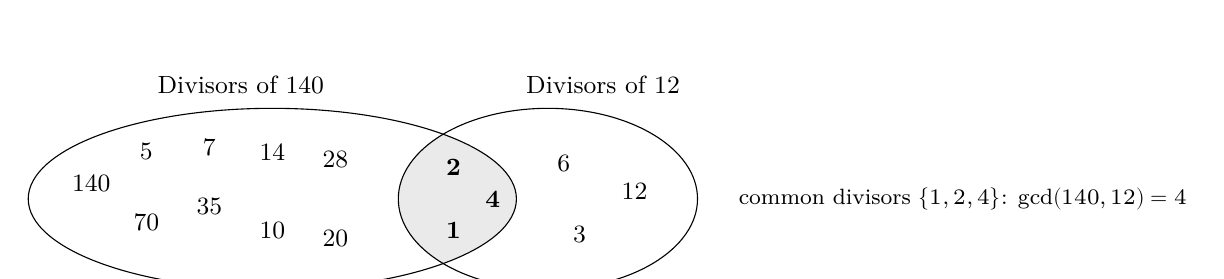
\begin{tikzpicture}[font=\small]
  \begin{scope}
    \clip (0,0) ellipse (3.1 and 1.15);
    \fill[gray!18] (3.5,0) ellipse (1.9 and 1.15);
  \end{scope}
  \draw (0,0) ellipse (3.1 and 1.15);
  \draw (3.5,0) ellipse (1.9 and 1.15);
  \node at (-0.4,1.45) {Divisors of 140};
  \node at (4.2,1.45) {Divisors of 12};
  \foreach \x/\y/\v in {-2.3/0.2/140,-1.6/0.6/5,-1.6/-0.3/70,-0.8/0.65/7,-0.8/-0.1/35,0/0.6/14,0/-0.4/10,0.8/0.5/28,0.8/-0.5/20}{\node at (\x,\y) {\v};}
  \foreach \x/\y/\v in {2.3/0.4/2,2.3/-0.4/1,2.8/0/4}{\node[font=\small\bfseries] at (\x,\y) {\v};}
  \foreach \x/\y/\v in {3.7/0.45/6,3.9/-0.45/3,4.6/0.1/12}{\node at (\x,\y) {\v};}
  \node[anchor=west] at (5.8,0) {\footnotesize common divisors $\{1, 2, 4\}$: $\gcd(140, 12) = 4$};
\end{tikzpicture}
\end{center}

\subsection{Euclid's algorithm and why it works}
The algorithm rests on two facts stated on the slides.
\[
\textbf{Fact 1: } \gcd(a, 0) = a, \qquad\qquad \textbf{Fact 2: } \gcd(a, b) = \gcd(b, r), \text{ where } r = a \bmod b .
\]
\textbf{Why Fact 1 holds.} Every integer divides 0 (since $0 = 0 \times d$), so the common divisors of $a$ and 0 are just the divisors of $a$, and the largest of these is $a$ itself.

\textbf{Why Fact 2 holds.} Divide: $a = qb + r$. If $d$ divides both $a$ and $b$, then by Property 4 it divides $a - qb = r$. Conversely, if $d$ divides both $b$ and $r$, then it divides $qb + r = a$. The pairs $(a, b)$ and $(b, r)$ therefore have exactly the same set of common divisors, and so the same greatest common divisor. The argument works for any multiple $qb$; the remainder is used because it makes the new pair as small as possible.

\textbf{The algorithm.} Apply Fact 2 repeatedly, replacing $(a, b)$ by $(b, a \bmod b)$, until the second number is 0; then Fact 1 gives the answer. The slide's example:
\[
\gcd(36, 10) = \gcd(10, 6) = \gcd(6, 4) = \gcd(4, 2) = \gcd(2, 0) = \mathbf{2}.
\]
\textbf{Termination.} Each step replaces the second number $b$ by $r = a \bmod b$, and $0 \le r < b$. The second numbers therefore form a strictly decreasing sequence of non-negative integers, $b > r_1 > r_2 > \cdots$, which must reach 0 after at most $b$ steps; the last non-zero term is the gcd.

\textbf{Speed.} The bound of $b$ steps is far too pessimistic: the remainder at least halves every two steps. Consider three consecutive remainders, where $r_{i+2} = r_i \bmod r_{i+1}$. If $r_{i+1} \le r_i / 2$, then $r_{i+2} < r_{i+1} \le r_i / 2$. Otherwise $r_{i+1} > r_i / 2$, the quotient is 1, and $r_{i+2} = r_i - r_{i+1} < r_i / 2$. Either way two steps halve the remainder, so at most about $2\log_2 b$ divisions are needed, which is linear in the number of digits. A 1024-bit $b$ therefore needs at most about 2048 divisions, while listing divisors would need about $2^{1024}$ trial divisions. The slowest inputs are consecutive Fibonacci numbers, where every quotient is 1: $\gcd(89, 55)$ takes 9 divisions.

Forouzan writes the algorithm with two variables $r_1$ and $r_2$ that hold the current pair:
\begin{center}
\begin{minipage}{0.55\textwidth}
\small\ttfamily
r$_1$ $\leftarrow$ a;\quad r$_2$ $\leftarrow$ b;\hfill\textrm{(initialisation)}\\
while (r$_2$ > 0)\\
\{\\
\hspace*{1.5em}q $\leftarrow$ r$_1$ / r$_2$;\hfill\textrm{(integer quotient)}\\
\hspace*{1.5em}r $\leftarrow$ r$_1$ $-$ q $\times$ r$_2$;\\
\hspace*{1.5em}r$_1$ $\leftarrow$ r$_2$;\quad r$_2$ $\leftarrow$ r;\\
\}\\
gcd(a, b) $\leftarrow$ r$_1$
\end{minipage}
\end{center}

\begin{mustknow}
$\gcd(a, b) = \gcd(b,\ a \bmod b)$ and $\gcd(a, 0) = a$. Divide, shift ($B \to A$, $R \to B$), and stop when the second number is 0: the gcd is the last non-zero remainder. At most about $2\log_2 b$ divisions.
\end{mustknow}

\subsection{Method 1: the table (Q, A, B, R)}
The lecture video lays the divisions out as a table, which is the format to use in an exam.
\begin{enumerate}[leftmargin=1.5em,itemsep=1pt]
  \item Draw the columns $Q$ (quotient), $A$, $B$ and $R$ (remainder), and start with $A$ = the larger number and $B$ = the smaller.
  \item In each row compute $Q = \lfloor A/B \rfloor$ and $R = A \bmod B$, so that $A = Q \times B + R$.
  \item In the next row $B$ moves into $A$ and $R$ moves into $B$ (the diagonal arrows below). This is Fact 2.
  \item Stop when $B = 0$, since division by 0 is impossible; write X for $Q$ and $R$. The gcd is the $A$ of that row (Fact 1).
\end{enumerate}
\begin{center}
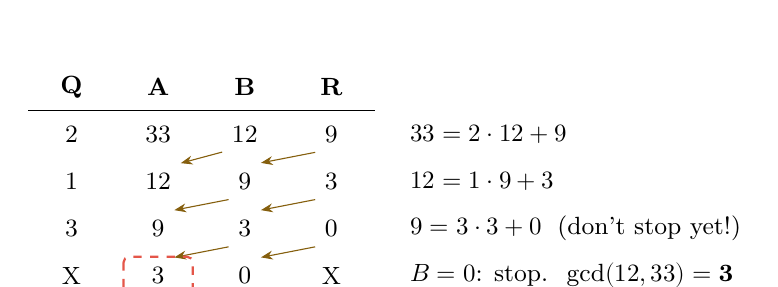
\begin{tikzpicture}[x=11mm,y=6mm]
  \foreach \h [count=\c] in {Q,A,B,R}{\node[font=\small\bfseries] at (\c,0) {\h};}
  \draw (0.5,-0.5) -- (4.5,-0.5);
  \foreach \q/\a/\b/\r [count=\i] in {2/33/12/9, 1/12/9/3, 3/9/3/0, X/3/0/X}{
    \node[font=\small] at (1,-\i) {\q};
    \node[font=\small] (a\i) at (2,-\i) {\a};
    \node[font=\small] (b\i) at (3,-\i) {\b};
    \node[font=\small] (r\i) at (4,-\i) {\r};
  }
  \foreach \i in {1,2,3}{\pgfmathtruncatemacro{\j}{\i+1}
    \draw[-{Stealth[length=1.5mm]},orange!80!black] (b\i.south west) -- (a\j.north east);
    \draw[-{Stealth[length=1.5mm]},orange!80!black] (r\i.south west) -- (b\j.north east);}
  \draw[warn,thick,dashed,rounded corners=2pt] (1.6,-3.6) rectangle (2.4,-4.4);
  \node[font=\small,anchor=west] at (4.8,-1) {$33 = 2\cdot12 + 9$};
  \node[font=\small,anchor=west] at (4.8,-2) {$12 = 1\cdot9 + 3$};
  \node[font=\small,anchor=west] at (4.8,-3) {$9 = 3\cdot3 + 0$ \;(don't stop yet!)};
  \node[font=\small,anchor=west] at (4.8,-4) {$B = 0$: stop. \;$\gcd(12, 33) = \mathbf{3}$};
\end{tikzpicture}
\end{center}
The other lecture examples, and Forouzan's slide example with the columns named $q, r_1, r_2, r$ (the same table under different names):
\begin{center}\small
\begin{minipage}[t]{0.27\textwidth}
\centering
$\gcd(750, 900)$\\[2pt]
\begin{tabular}{cccc}
\toprule
Q&A&B&R\\
\midrule
1&900&750&150\\
5&750&150&0\\
X&\textbf{150}&0&X\\
\bottomrule
\end{tabular}
\end{minipage}\hfill
\begin{minipage}[t]{0.27\textwidth}
\centering
$\gcd(252, 105)$\\[2pt]
\begin{tabular}{cccc}
\toprule
Q&A&B&R\\
\midrule
2&252&105&42\\
2&105&42&21\\
2&42&21&0\\
X&\textbf{21}&0&X\\
\bottomrule
\end{tabular}
\end{minipage}\hfill
\begin{minipage}[t]{0.36\textwidth}
\centering
$\gcd(2740, 1760)$ (Lecture 2)\\[2pt]
\begin{tabular}{cccc}
\toprule
$q$&$r_1$&$r_2$&$r$\\
\midrule
1&2740&1760&980\\
1&1760&980&780\\
1&980&780&200\\
3&780&200&180\\
1&200&180&20\\
9&180&20&0\\
&\textbf{20}&0&\\
\bottomrule
\end{tabular}
\end{minipage}
\end{center}
\textbf{Shortcut.} The gcd is the \textbf{last non-zero remainder} (9, 3, \textbf{3}, then 0; or 42, \textbf{21}, then 0). The extra row with $B = 0$ is only where the lecture reads it off. The Lecture 2 class exercise, $\gcd(25, 60)$, runs $60 = 2 \times 25 + 10$, $25 = 2 \times 10 + 5$, $10 = 2 \times 5 + 0$, giving $\mathbf{5}$.

\subsection{Method 2: recursion}
Facts 1 and 2 are already a recursive definition, and the second lecture video writes them as a function:
\begin{center}
\begin{minipage}{0.45\textwidth}
\small\ttfamily
Prerequisite: a > b\\
Euclid\_GCD(a, b):\\
\hspace*{1.5em}if b = 0 then\\
\hspace*{3em}return a;\hfill\textrm{(Fact 1)}\\
\hspace*{1.5em}else\\
\hspace*{3em}return Euclid\_GCD(b, a mod b);\hfill\textrm{(Fact 2)}
\end{minipage}
\end{center}
\begin{minipage}[t]{0.42\textwidth}
\small
\textbf{$\gcd(50, 12)$}\\
$= \gcd(12, 50 \bmod 12) = \gcd(12, 2)$\\
$= \gcd(2, 12 \bmod 2) = \gcd(2, 0)$\\
$= \mathbf{2}$
\end{minipage}\hfill
\begin{minipage}[t]{0.55\textwidth}
\small
\textbf{$\gcd(83, 19)$}\\
$= \gcd(19, 7)$ \quad ($83 = 4\cdot19 + 7$)\\
$= \gcd(7, 5)$ \quad ($19 = 2\cdot7 + 5$)\\
$= \gcd(5, 2)$ \quad ($7 = 1\cdot5 + 2$)\\
$= \gcd(2, 1)$ \quad ($5 = 2\cdot2 + 1$)\\
$= \gcd(1, 0) = \mathbf{1}$ \quad ($2 = 2\cdot1 + 0$)
\end{minipage}

\medskip
Both methods perform exactly the same divisions, so either may be used. The prerequisite $a > b$ is a convenience, not a necessity. If the smaller number comes first, the first call swaps them at the cost of one wasted step: $\gcd(12, 33) \to \gcd(33, 12 \bmod 33) = \gcd(33, 12)$, since $12 \bmod 33 = 12$. In the exam it is cleaner to write the larger number first.

\subsection{Relatively prime numbers}
\imp{Two integers $a$ and $b$ are relatively prime (co-prime) if $\gcd(a, b) = 1$}, as for 83 and 19 above. The condition is about the pair: neither number has to be prime, as $\gcd(8, 9) = 1$ shows. Cryptography needs the notion for three reasons. First, $a^{-1} \bmod n$ exists only if $\gcd(a, n) = 1$ (\S\ref{sec:modular}); this is the Hill key condition $\gcd(\det K, 26) = 1$ and the affine-cipher condition on the multiplier. Second, RSA key generation chooses $e$ with $\gcd(e, \phi(n)) = 1$, so that $d = e^{-1} \bmod \phi(n)$ exists. Third, the number of residues co-prime to $n$ is Euler's totient $\phi(n)$ (\S\ref{sec:totient}). Euclid's algorithm decides co-primality; the extended algorithm (\S\ref{sec:exteuclid}) runs the same divisions while tracking two extra columns and produces the inverse itself, instead of the trial-and-error table used for $23^{-1} \bmod 26$ in the Hill cipher.

\begin{worked}[: GCD by the Euclidean algorithm (Forouzan exercise)]
\textbf{Q.} Find (a) $\gcd(88, 220)$ \quad (b) $\gcd(300, 42)$ \quad (c) $\gcd(24, 320)$ \quad (d) $\gcd(401, 700)$. Which pairs are relatively prime?

\textbf{A.} Larger number first; each line is one row $A = Q \times B + R$.
\begin{center}\small
\begin{tabular}{@{}lll@{}}
\toprule
Pair & Divisions & gcd\\
\midrule
(a) 220, 88 & $220 = 2 \times 88 + 44$, \;$88 = 2 \times 44 + 0$ & \textbf{44}\\
(b) 300, 42 & $300 = 7 \times 42 + 6$, \;$42 = 7 \times 6 + 0$ & \textbf{6}\\
(c) 320, 24 & $320 = 13 \times 24 + 8$, \;$24 = 3 \times 8 + 0$ & \textbf{8}\\
\bottomrule
\end{tabular}
\end{center}
(d) needs a longer table:
\begin{center}\small
\begin{tabular}{cccc|l}
\toprule
Q&A&B&R&\\
\midrule
1&700&401&299&$700 = 1 \times 401 + 299$\\
1&401&299&102&$401 = 1 \times 299 + 102$\\
2&299&102&95&$299 = 2 \times 102 + 95$\\
1&102&95&7&$102 = 1 \times 95 + 7$\\
13&95&7&4&$95 = 13 \times 7 + 4$\\
1&7&4&3&$7 = 1 \times 4 + 3$\\
1&4&3&1&$4 = 1 \times 3 + 1$\\
3&3&1&0&$3 = 3 \times 1 + 0$\\
X&\textbf{1}&0&X&\\
\bottomrule
\end{tabular}
\end{center}
\textbf{Answers: 44, 6, 8, 1.} Only 401 and 700 are relatively prime, so 401 has an inverse modulo 700 and the other pairs have none. \textbf{Check:} $88 = 2 \times 44$ and $220 = 5 \times 44$ with $\gcd(2, 5) = 1$; similarly $300 = 50 \times 6$, $42 = 7 \times 6$ and $320 = 40 \times 8$, $24 = 3 \times 8$, with co-prime cofactors.
\end{worked}

\textbf{Lecture homework:} $\gcd(1005, 105)$ (table method) and $\gcd(529, 123)$ (recursive method). Solutions are in practice Q43.

\begin{trap}[: reading the table]
\begin{itemize}[leftmargin=1.5em]
  \item Stop when $B = 0$, not when $R = 0$. In the row where $R$ first becomes 0, the answer is that row's $B$, which moves into $A$ in the next row; reading $A$ from the row with $R = 0$ gives a wrong answer (9 instead of 3 for $\gcd(33, 12)$).
  \item Swapping the meaning of the two outputs: ``$A \bmod B$'' gives the remainder $R$, while ``$A$ divided by $B$'' gives the quotient $Q$. The table needs both.
  \item Show every division as $A = Q \times B + R$ in the exam; the marks are for the steps, not only for the final number.
\end{itemize}
\end{trap}

\begin{fixbox}
\begin{itemize}
  \item All results are correct (checked by script): 3, 25, 1, 3, 150, 21, 2, 1 from the videos, and $\gcd(36, 10) = 2$, $\gcd(2740, 1760) = 20$, $\gcd(25, 60) = 5$, $\gcd(140, 12) = 4$ from the Lecture 2 slides.
  \item Verbal slips only: ``divisors of 13'' means 33 (video 1); ``a = 9'' means 19 (video 2). The slides are right.
  \item Wording: ``$A$ mod $B$'' gives the \emph{remainder}; ``$A$ divided by $B$'' gives the quotient $Q$. The table needs both.
\end{itemize}
\end{fixbox}

% College Lecture 2 (extended Euclid: process, algorithm, 161/28, 17/0, 0/45, 84/320) + Lecture 4 (inverse with the t columns,
% 11/26, 23/100, 12/26; linear Diophantine equations), Forouzan 2.1--2.2. All tables generated by script (scratchpad/r4/verify.py).
\section{Extended Euclidean Algorithm \hothot}\label{sec:exteuclid}
\asked{Mid-sem 2024--25 Q7 (5 marks): pseudocode + $23^{-1}$ in $\mathbb{Z}_{100}$ with ``value in iteration $k$'' sub-questions. 2025--26 Q5 (3 marks): solve $19x + 13y = 20$. The same table, with polynomials, gives the GF$(2^8)$ inverse asked in both years (\S\ref{sec:algebra}), and $d$ in RSA (\S\ref{sec:rsa}).}

Euclid's algorithm decides whether $\gcd(a, n) = 1$, and hence whether $a^{-1} \bmod n$ exists, but it does not produce the inverse. The extended Euclidean algorithm does. \imp{Given two integers $a$ and $b$, the extended Euclidean algorithm computes $\gcd(a, b)$ and, at the same time, integers $s$ and $t$ such that $s \times a + t \times b = \gcd(a, b)$.} That such $s$ and $t$ always exist is \textbf{Bézout's identity}; the algorithm proves it by constructing them. One table then answers four kinds of exam question: the inverse $b^{-1} \bmod n$, the solutions of a linear Diophantine equation $ax + by = c$, the solutions of a linear congruence (\S\ref{sec:modular}), and the RSA private key $d = e^{-1} \bmod \phi(n)$. With polynomials instead of integers the same table gives inverses in GF$(2^8)$.

\subsection{The idea: carry every remainder as a combination of \texorpdfstring{$a$ and $b$}{a and b}}
By hand, $s$ and $t$ can be found by back-substitution. For $a = 19$ and $b = 13$, Euclid's divisions are $19 = 1 \times 13 + 6$ and $13 = 2 \times 6 + 1$. Solving them from the last line upwards gives
\[
1 = 13 - 2 \times 6 = 13 - 2 \times (19 - 1 \times 13) = 3 \times 13 - 2 \times 19,
\]
so $s = -2$ and $t = 3$. This works, but it requires storing every quotient, running the divisions a second time in reverse, and keeping track of signs, which is where most errors happen. The extended algorithm does the same bookkeeping forwards, in a single pass.

The key observation is that every remainder in Euclid's sequence is an integer combination of $a$ and $b$. The first two numbers of the sequence are $a$ and $b$ themselves, and trivially
\[
r_1 = a = 1 \cdot a + 0 \cdot b, \qquad r_2 = b = 0 \cdot a + 1 \cdot b,
\]
which gives the starting values $s_1 = 1$, $s_2 = 0$, $t_1 = 0$, $t_2 = 1$. Suppose that in some row the \textbf{invariant} $r_1 = s_1 a + t_1 b$ and $r_2 = s_2 a + t_2 b$ holds. The next remainder is $r = r_1 - q r_2$, and substituting the two combinations gives
\[
r = (s_1 a + t_1 b) - q\,(s_2 a + t_2 b) = (s_1 - q s_2)\,a + (t_1 - q t_2)\,b .
\]
So if $s$ and $t$ are updated by exactly the same rule as $r$, namely $s = s_1 - q s_2$ and $t = t_1 - q t_2$, the new remainder satisfies $r = s a + t b$. After the shift $(r_1, r_2) \leftarrow (r_2, r)$, $(s_1, s_2) \leftarrow (s_2, s)$, $(t_1, t_2) \leftarrow (t_2, t)$ the invariant holds again, so by induction it holds in every row. The $r$ columns are Euclid's algorithm unchanged, so the loop ends with $r_1 = \gcd(a, b)$ and $r_2 = 0$, and the invariant for $r_1$ then reads $\gcd(a, b) = s_1 a + t_1 b$. This proves Bézout's identity for all $a$ and $b$.

\subsection{The algorithm and the table (Forouzan)}
The slides give the algorithm as three identical update blocks, one for each pair of variables:
\begin{center}
\begin{minipage}{0.62\textwidth}
\small\ttfamily
r$_1$ $\leftarrow$ a;\quad r$_2$ $\leftarrow$ b;\\
s$_1$ $\leftarrow$ 1;\quad s$_2$ $\leftarrow$ 0;\hfill\textrm{(initialisation)}\\
t$_1$ $\leftarrow$ 0;\quad t$_2$ $\leftarrow$ 1;\\
while (r$_2$ > 0)\\
\{\\
\hspace*{1.5em}q $\leftarrow$ r$_1$ / r$_2$;\\
\hspace*{1.5em}r $\leftarrow$ r$_1$ $-$ q $\times$ r$_2$;\quad r$_1$ $\leftarrow$ r$_2$;\quad r$_2$ $\leftarrow$ r;\hfill\textrm{(updating r's)}\\
\hspace*{1.5em}s $\leftarrow$ s$_1$ $-$ q $\times$ s$_2$;\quad s$_1$ $\leftarrow$ s$_2$;\quad s$_2$ $\leftarrow$ s;\hfill\textrm{(updating s's)}\\
\hspace*{1.5em}t $\leftarrow$ t$_1$ $-$ q $\times$ t$_2$;\quad t$_1$ $\leftarrow$ t$_2$;\quad t$_2$ $\leftarrow$ t;\hfill\textrm{(updating t's)}\\
\}\\
gcd(a, b) $\leftarrow$ r$_1$;\quad s $\leftarrow$ s$_1$;\quad t $\leftarrow$ t$_1$
\end{minipage}
\end{center}
On paper each pass of the loop is one row of a table with the columns $q \mid r_1\ r_2\ r \mid s_1\ s_2\ s \mid t_1\ t_2\ t$. In every row the three blocks do the same thing: the new value is (first) $-\ q \times$ (second), and in the next row the second value moves into the first column and the new value into the second. A final row, with no quotient, shows the values after the loop, and the answer is read from its \emph{first} columns. The slide example, $a = 161$, $b = 28$:
\begin{center}\small
\begin{tabular}{@{}r|rrr|rrr|rrr@{}}
\toprule
$q$ & $r_1$ & $r_2$ & $r$ & $s_1$ & $s_2$ & $s$ & $t_1$ & $t_2$ & $t$\\
\midrule
5 & 161 & 28 & 21 & 1 & 0 & 1 & 0 & 1 & $-5$\\
1 & 28 & 21 & 7 & 0 & 1 & $-1$ & 1 & $-5$ & 6\\
3 & 21 & 7 & 0 & 1 & $-1$ & 4 & $-5$ & 6 & $-23$\\
 & \textbf{7} & 0 & & $\mathbf{-1}$ & 4 & & \textbf{6} & $-23$ & \\
\bottomrule
\end{tabular}
\end{center}
$\gcd(161, 28) = 7$, $s = -1$, $t = 6$: \;$(-1)(161) + 6(28) = -161 + 168 = 7$ \checkmark. The invariant can be checked in every row: $21 = 1 \times 161 - 5 \times 28$, $7 = -1 \times 161 + 6 \times 28$ and $0 = 4 \times 161 - 23 \times 28$. The last of these gives a free self-check: in the final row $s_2 a + t_2 b = 0$, and $(s_2, t_2)$ always equals $\pm(b/d, -a/d)$ with $d = \gcd(a, b)$; here $(4, -23) = (28/7, -161/7)$. In an inverse table (next subsection) this means the final $t_2$ is $\pm n$, so any other value there reveals an arithmetic slip.

The other slide examples test the edge cases. For $a = 17$, $b = 0$ the loop never runs, because $r_2 = 0$ from the start, and the initial values give $\gcd(17, 0) = 17$, $s = 1$, $t = 0$. For $a = 0$, $b = 45$ one iteration with $q = 0$ swaps the pair, giving $\gcd(0, 45) = 45$, $s = 0$, $t = 1$. The slide exercise $a = 84$, $b = 320$ also starts with the smaller number, and the first row ($q = 0$) simply swaps it:
\begin{center}\small
\begin{tabular}{@{}r|rrr|rrr|rrr@{}}
\toprule
$q$ & $r_1$ & $r_2$ & $r$ & $s_1$ & $s_2$ & $s$ & $t_1$ & $t_2$ & $t$\\
\midrule
0 & 84 & 320 & 84 & 1 & 0 & 1 & 0 & 1 & 0\\
3 & 320 & 84 & 68 & 0 & 1 & $-3$ & 1 & 0 & 1\\
1 & 84 & 68 & 16 & 1 & $-3$ & 4 & 0 & 1 & $-1$\\
4 & 68 & 16 & 4 & $-3$ & 4 & $-19$ & 1 & $-1$ & 5\\
4 & 16 & 4 & 0 & 4 & $-19$ & 80 & $-1$ & 5 & $-21$\\
 & \textbf{4} & 0 & & $\mathbf{-19}$ & 80 & & \textbf{5} & $-21$ & \\
\bottomrule
\end{tabular}
\end{center}
$\gcd(84, 320) = 4$, $s = -19$, $t = 5$: \;$-19 \times 84 + 5 \times 320 = -1596 + 1600 = 4$ \checkmark, as on the slide. The final $(s_2, t_2) = (80, -21) = (320/4, -84/4)$ confirms it.

\subsection{Multiplicative inverse with the table \hothot}
\likely{``Find $b^{-1}$ in $\mathbb{Z}_n$ using the extended Euclidean algorithm; give the number of iterations / $r$ or $t$ in iteration $k$'' (5 marks), and $d = e^{-1} \bmod \phi(n)$ in every RSA question.}
To find $b^{-1} \bmod n$, run the algorithm with $a = n$, that is, $r_1 = n$ and $r_2 = b$. At the end $s \times n + t \times b = \gcd(n, b)$. If the gcd is 1, reduce this equation modulo $n$; the slides do it in three lines:
\[
(s \times n + b \times t) \bmod n = 1 \;\Rightarrow\; [(s \times n) \bmod n] + [(b \times t) \bmod n] = 1 \;\Rightarrow\; (b \times t) \bmod n = 1 .
\]
So \imp{the multiplicative inverse of $b$ is the final $t_1$, mapped into $\mathbb{Z}_n$}. The $s$ columns are never used and are dropped, leaving $q \mid r_1\ r_2\ r \mid t_1\ t_2\ t$. If the final $r_1$ is not 1, then $\gcd(n, b) > 1$ and no inverse exists (\S\ref{sec:modular}); the algorithm detects this by itself. A negative $t_1$ is normal and is mapped into $\mathbb{Z}_n$ by adding $n$. The slide's version of the algorithm, which is the pseudocode asked in 2024--25 Q7:
\begin{center}
\begin{minipage}{0.56\textwidth}
\small\ttfamily
r$_1$ $\leftarrow$ n;\quad r$_2$ $\leftarrow$ b;\quad t$_1$ $\leftarrow$ 0;\quad t$_2$ $\leftarrow$ 1;\\
while (r$_2$ > 0)\\
\{\\
\hspace*{1.5em}q $\leftarrow$ r$_1$ / r$_2$;\\
\hspace*{1.5em}r $\leftarrow$ r$_1$ $-$ q $\times$ r$_2$;\quad r$_1$ $\leftarrow$ r$_2$;\quad r$_2$ $\leftarrow$ r;\\
\hspace*{1.5em}t $\leftarrow$ t$_1$ $-$ q $\times$ t$_2$;\quad t$_1$ $\leftarrow$ t$_2$;\quad t$_2$ $\leftarrow$ t;\\
\}\\
if (r$_1$ = 1) then b$^{-1}$ $\leftarrow$ t$_1$ mod n\\
else ``no inverse''
\end{minipage}
\end{center}
The three slide examples:
\begin{center}\small
\begin{tabular}{@{}r|rrr|rrr@{}}
\multicolumn{7}{c}{$11^{-1} \bmod 26$}\\
\toprule
$q$ & $r_1$ & $r_2$ & $r$ & $t_1$ & $t_2$ & $t$\\
\midrule
2 & 26 & 11 & 4 & 0 & 1 & $-2$\\
2 & 11 & 4 & 3 & 1 & $-2$ & 5\\
1 & 4 & 3 & 1 & $-2$ & 5 & $-7$\\
3 & 3 & 1 & 0 & 5 & $-7$ & 26\\
 & \textbf{1} & 0 & & $\mathbf{-7}$ & 26 & \\
\bottomrule
\end{tabular}
\quad
\begin{tabular}{@{}r|rrr|rrr@{}}
\multicolumn{7}{c}{$23^{-1} \bmod 100$}\\
\toprule
$q$ & $r_1$ & $r_2$ & $r$ & $t_1$ & $t_2$ & $t$\\
\midrule
4 & 100 & 23 & 8 & 0 & 1 & $-4$\\
2 & 23 & 8 & 7 & 1 & $-4$ & 9\\
1 & 8 & 7 & 1 & $-4$ & 9 & $-13$\\
7 & 7 & 1 & 0 & 9 & $-13$ & 100\\
 & \textbf{1} & 0 & & $\mathbf{-13}$ & 100 & \\
\bottomrule
\end{tabular}
\quad
\begin{tabular}{@{}r|rrr|rrr@{}}
\multicolumn{7}{c}{$12^{-1} \bmod 26$}\\
\toprule
$q$ & $r_1$ & $r_2$ & $r$ & $t_1$ & $t_2$ & $t$\\
\midrule
2 & 26 & 12 & 2 & 0 & 1 & $-2$\\
6 & 12 & 2 & 0 & 1 & $-2$ & 13\\
 & \textbf{2} & 0 & & $-2$ & 13 & \\
\bottomrule
\end{tabular}
\end{center}
$11^{-1} \equiv -7 \equiv \mathbf{19} \pmod{26}$ (check: $11 \times 19 = 209 = 8 \times 26 + 1$); \;$23^{-1} \equiv -13 \equiv \mathbf{87} \pmod{100}$ (check: $23 \times 87 = 2001$); \;$12^{-1} \bmod 26$: the final $r_1 = 2$, so $\gcd(26, 12) = 2$ and \textbf{no inverse exists}. In the third table $t_1 = -2$ still satisfies $12 \times (-2) \equiv 2 \pmod{26}$, the gcd rather than 1, which is exactly what the invariant predicts.

\begin{worked}[: 2024--25 Q7 (5 marks), inverse with ``iteration $k$'' sub-questions]
\textbf{Q.} Write the pseudocode for finding the multiplicative inverse of $b$ in $\mathbb{Z}_n$, and use it to find $23^{-1}$ in $\mathbb{Z}_{100}$. State (a) the number of iterations, (b) the remainder in iteration 2, (c) the value of $t$ in iteration 4, (d) the iteration whose $t$ becomes the inverse.

\textbf{A.} Pseudocode: as above ($r_1 = n$, $r_2 = b$, $t_1 = 0$, $t_2 = 1$; loop while $r_2 > 0$; inverse $= t_1 \bmod n$ if $r_1 = 1$). An \emph{iteration} is one pass of the while loop, i.e.\ one row that has a quotient; the row shows the values at the start of the pass and the $r$, $t$ computed in it.
\begin{center}\small
\begin{tabular}{@{}c|c|rrr|rrr@{}}
\toprule
Iteration & $q$ & $r_1$ & $r_2$ & $r$ & $t_1$ & $t_2$ & $t$\\
\midrule
1 & 4 & 100 & 23 & 8 & 0 & 1 & $-4$\\
2 & 2 & 23 & 8 & \textbf{7} & 1 & $-4$ & 9\\
3 & 1 & 8 & 7 & 1 & $-4$ & 9 & $\mathbf{-13}$\\
4 & 7 & 7 & 1 & 0 & 9 & $-13$ & \textbf{100}\\
(end) & & \textbf{1} & 0 & & $\mathbf{-13}$ & 100 & \\
\bottomrule
\end{tabular}
\end{center}
Since $r_1 = 1$, $\gcd(100, 23) = 1$ and the inverse exists. (a) \textbf{4 iterations}. (b) The remainder in iteration 2 is $\mathbf{7}$ ($23 = 2 \times 8 + 7$). (c) $t$ in iteration 4 is $\mathbf{100}$, which is $\pm n$ as the self-check predicts. (d) Iteration 3 computes $t = -13$, which becomes the final $t_1$; mapped into $\mathbb{Z}_{100}$: $23^{-1} = -13 + 100 = \mathbf{87}$.
\textbf{Check:} $23 \times 87 = 2001 = 20 \times 100 + 1$ \checkmark.
\end{worked}

\begin{worked}[: inverse in $\mathbb{Z}_{180}$ (Forouzan exercise)]
\textbf{Q.} Using the extended Euclidean algorithm, find the multiplicative inverses of 7, 132 and 24 in $\mathbb{Z}_{180}$, where they exist.

\textbf{A.} For $b = 7$:
\begin{center}\small
\begin{tabular}{@{}c|c|rrr|rrr@{}}
\toprule
Iteration & $q$ & $r_1$ & $r_2$ & $r$ & $t_1$ & $t_2$ & $t$\\
\midrule
1 & 25 & 180 & 7 & 5 & 0 & 1 & $-25$\\
2 & 1 & 7 & 5 & 2 & 1 & $-25$ & 26\\
3 & 2 & 5 & 2 & 1 & $-25$ & 26 & $-77$\\
4 & 2 & 2 & 1 & 0 & 26 & $-77$ & 180\\
(end) & & \textbf{1} & 0 & & $\mathbf{-77}$ & 180 & \\
\bottomrule
\end{tabular}
\end{center}
$r_1 = 1$, so the inverse exists: $7^{-1} = -77 + 180 = \mathbf{103}$. Check: $7 \times 103 = 721 = 4 \times 180 + 1$ \checkmark.
For $b = 132$ the $r$ columns run $180 = 1 \times 132 + 48$, $132 = 2 \times 48 + 36$, $48 = 1 \times 36 + 12$, $36 = 3 \times 12 + 0$, ending with $r_1 = 12 \ne 1$: \textbf{no inverse}. For $b = 24$: $180 = 7 \times 24 + 12$, $24 = 2 \times 12 + 0$, again $r_1 = 12$: \textbf{no inverse}. Both share the factor 12 with 180.
\end{worked}

\subsection{Linear Diophantine equations \texorpdfstring{$ax + by = c$}{ax + by = c} \hot}
\likely{``Find the particular and general solutions of $ax + by = c$'' (3 marks), as in 2025--26 Q5; occasionally a word problem with non-negative solutions.}
\imp{A linear Diophantine equation in two variables is $ax + by = c$, where $a$, $b$, $c$ are integers and only integer solutions $x$, $y$ are wanted.} Over the reals such an equation has a whole line of solutions; restricting to integers leaves either none or infinitely many, and the extended Euclidean algorithm decides which and finds them all. The three facts below are derived from Bézout's identity, with $d = \gcd(a, b)$.

\textbf{No solution unless $d \mid c$.} For every pair of integers $x, y$, $d$ divides $ax + by$ (Property 4 of \S\ref{sec:gcd}). If $d \nmid c$, no choice of $x$, $y$ can make $ax + by$ equal to $c$. For example $15x + 12y = 13$ has no solution, because $\gcd(15, 12) = 3$ and $3 \nmid 13$.

\textbf{A particular solution when $d \mid c$.} Divide the equation by $d$: $a'x + b'y = c'$ with $a' = a/d$, $b' = b/d$, $c' = c/d$ and $\gcd(a', b') = 1$. The extended algorithm on $(a', b')$ gives $s$ and $t$ with $a's + b't = 1$, and multiplying by $c'$ gives $a'(c's) + b'(c't) = c'$. So $x_0 = (c/d)\,s$, $y_0 = (c/d)\,t$ is a solution. (Running the algorithm on $(a, b)$ directly gives the same $s$, $t$, since $sa + tb = d$ is the same equation multiplied by $d$.)

\textbf{The general solution.} Let $(x, y)$ be any other solution. Subtracting $a'x_0 + b'y_0 = c'$ from $a'x + b'y = c'$ gives $a'(x - x_0) = b'(y_0 - y)$. So $b'$ divides $a'(x - x_0)$, and since $b'$ is co-prime to $a'$, it divides $x - x_0$. (This step, \emph{Euclid's lemma}, follows from Bézout as well: multiplying $a's + b't = 1$ by $m = x - x_0$ gives $m = s\,a'm + t\,b'm$, and $b'$ divides both terms.) Hence $x = x_0 + k b'$ for some integer $k$, and substituting back gives $y = y_0 - k a'$. Conversely every $k$ gives a solution, because $a'(x_0 + kb') + b'(y_0 - ka') = a'x_0 + b'y_0$. These are the slide's formulas:
\[
\text{particular: } x_0 = \frac{c}{d}\,s, \quad y_0 = \frac{c}{d}\,t, \qquad\qquad
\text{general: } x = x_0 + k\,\frac{b}{d}, \quad y = y_0 - k\,\frac{a}{d}, \quad k \in \mathbb{Z}.
\]
The solutions are evenly spaced: $x$ steps by $b/d$ while $y$ steps by $a/d$ in the opposite direction, which keeps $ax + by$ constant. The linear congruence $ax \equiv b \pmod n$ of \S\ref{sec:modular} is the same problem in disguise, since it means $ax + ny = b$ for some integer $y$; the condition $d \mid b$ and the spacing $n/d$ of its $d$ solutions are this result read modulo $n$.

\begin{mustknow}
$s \cdot a + t \cdot b = \gcd(a, b)$: update $r$, $s$, $t$ by the same rule (new $=$ first $- q \times$ second), stop when $r_2 = 0$, read $r_1$, $s_1$, $t_1$.
Inverse: run with $r_1 = n$, $r_2 = b$; if the final $r_1 = 1$, then $b^{-1} = t_1 \bmod n$, otherwise no inverse.
$ax + by = c$: solvable iff $d = \gcd(a, b) \mid c$; $x = \frac{c}{d}s + k\frac{b}{d}$, \;$y = \frac{c}{d}t - k\frac{a}{d}$.
\end{mustknow}

The slide examples. For $21x + 14y = 35$: $d = \gcd(21, 14) = 7$ and $7 \mid 35$, so there are infinitely many solutions. Dividing by 7 gives $3x + 2y = 5$, and the algorithm on $(3, 2)$ gives $s = 1$, $t = -1$. The particular solution is $x_0 = 5 \times 1 = 5$, $y_0 = 5 \times (-1) = -5$, and the general solution is $x = 5 + 2k$, $y = -5 - 3k$: $(5, -5), (7, -8), (9, -11), \dots$, each of which satisfies $21x + 14y = 35$.
For cashing a Rs.~100 cheque in Rs.~20 and Rs.~5 notes, $20x + 5y = 100$: $d = 5$ divides 100, the reduced equation is $4x + y = 20$, and $4s + t = 1$ gives $s = 0$, $t = 1$. The particular solution is $x_0 = 0 \times 20 = 0$, $y_0 = 1 \times 20 = 20$, and the general one is $x = k$, $y = 20 - 4k$. Only non-negative note counts make sense, so $0 \le k \le 5$: $(0, 20)$, $(1, 16)$, $(2, 12)$, $(3, 8)$, $(4, 4)$, $(5, 0)$.

\begin{worked}[: 2025--26 Q5 (3 marks), solve $19x + 13y = 20$]
\textbf{Q.} Find the particular and general solutions of $19x + 13y = 20$.

\textbf{A.} Run the extended Euclidean algorithm on $a = 19$, $b = 13$:
\begin{center}\small
\begin{tabular}{@{}r|rrr|rrr|rrr@{}}
\toprule
$q$ & $r_1$ & $r_2$ & $r$ & $s_1$ & $s_2$ & $s$ & $t_1$ & $t_2$ & $t$\\
\midrule
1 & 19 & 13 & 6 & 1 & 0 & 1 & 0 & 1 & $-1$\\
2 & 13 & 6 & 1 & 0 & 1 & $-2$ & 1 & $-1$ & 3\\
6 & 6 & 1 & 0 & 1 & $-2$ & 13 & $-1$ & 3 & $-19$\\
 & \textbf{1} & 0 & & $\mathbf{-2}$ & 13 & & \textbf{3} & $-19$ & \\
\bottomrule
\end{tabular}
\end{center}
$d = \gcd(19, 13) = 1$, $s = -2$, $t = 3$ (check: $-2 \times 19 + 3 \times 13 = -38 + 39 = 1$). Since $1 \mid 20$, solutions exist.

\textbf{Particular:} $x_0 = (c/d)\,s = 20 \times (-2) = \mathbf{-40}$, \;$y_0 = (c/d)\,t = 20 \times 3 = \mathbf{60}$. \;Check: $19(-40) + 13(60) = -760 + 780 = 20$ \checkmark.

\textbf{General:} $x = -40 + 13k$, \;$y = 60 - 19k$, \;$k \in \mathbb{Z}$.
\begin{center}\small
\begin{tabular}{@{}c|cccccc@{}}
\toprule
$k$ & 0 & 1 & 2 & 3 & 4 & 5\\
\midrule
$(x, y)$ & $(-40, 60)$ & $(-27, 41)$ & $(-14, 22)$ & $\mathbf{(-1, 3)}$ & $(12, -16)$ & $(25, -35)$\\
\bottomrule
\end{tabular}
\end{center}
The smallest solution is $(-1, 3)$ ($k = 3$), so the general solution can also be written $x = -1 + 13k$, $y = 3 - 19k$. Check: $19(-1) + 13(3) = -19 + 39 = 20$ \checkmark.
\end{worked}

\begin{worked}[: non-negative solutions (Forouzan-style word problem)]
\textbf{Q.} A post office sells only 39-cent and 15-cent stamps. Find the numbers of stamps a customer can buy to pay exactly \$2.70 of postage.

\textbf{A.} Let $x$ and $y$ be the numbers of 39-cent and 15-cent stamps: $39x + 15y = 270$, with $x, y \ge 0$. $d = \gcd(39, 15) = 3$ ($39 = 2 \times 15 + 9$, $15 = 1 \times 9 + 6$, $9 = 1 \times 6 + 3$, $6 = 2 \times 3$), and $3 \mid 270$. Dividing by 3: $13x + 5y = 90$.
\begin{center}\small
\begin{tabular}{@{}r|rrr|rrr|rrr@{}}
\toprule
$q$ & $r_1$ & $r_2$ & $r$ & $s_1$ & $s_2$ & $s$ & $t_1$ & $t_2$ & $t$\\
\midrule
2 & 13 & 5 & 3 & 1 & 0 & 1 & 0 & 1 & $-2$\\
1 & 5 & 3 & 2 & 0 & 1 & $-1$ & 1 & $-2$ & 3\\
1 & 3 & 2 & 1 & 1 & $-1$ & 2 & $-2$ & 3 & $-5$\\
2 & 2 & 1 & 0 & $-1$ & 2 & $-5$ & 3 & $-5$ & 13\\
 & \textbf{1} & 0 & & \textbf{2} & $-5$ & & $\mathbf{-5}$ & 13 & \\
\bottomrule
\end{tabular}
\end{center}
$s = 2$, $t = -5$ ($2 \times 13 - 5 \times 5 = 1$). Particular: $x_0 = 90 \times 2 = 180$, $y_0 = 90 \times (-5) = -450$. General: $x = 180 + 5k$, $y = -450 - 13k$.
Non-negative counts need $180 + 5k \ge 0$, i.e.\ $k \ge -36$, and $-450 - 13k \ge 0$, i.e.\ $k \le -34.6$, so $k \in \{-36, -35\}$.
\textbf{Answer: $(x, y) = (0, 18)$ or $(5, 5)$}: eighteen 15-cent stamps, or five of each. Check: $15 \times 18 = 270$ and $39 \times 5 + 15 \times 5 = 195 + 75 = 270$ \checkmark.
\end{worked}

\begin{trap}[: where marks are lost]
\begin{itemize}[leftmargin=1.5em]
  \item For an inverse, put the \textbf{modulus first} ($r_1 = n$). Starting with $r_1 = b$ makes the inverse appear in the $s$ column, which the $t$-only table has dropped.
  \item Read the answer from the final row's \emph{first} columns ($r_1$, $s_1$, $t_1$), not from $t_2$ (which is $\pm n$) or from the last computed $t$.
  \item A negative $t_1$ is not an error: add $n$ (in RSA, add $\phi(n)$, never $n$). Check $b \times b^{-1} \bmod n = 1$ before writing the answer.
  \item If the final $r_1 \ne 1$, write ``no inverse, since $\gcd = r_1$''; do not report $t_1$.
  \item Show the full table with headed columns; the marks are awarded per row, and the ``iteration $k$'' sub-questions can only be answered from it.
\end{itemize}
\end{trap}

\begin{fixbox}
\begin{itemize}
  \item All slide tables are correct (recomputed by script): $(161, 28) \to 7, -1, 6$; $(17, 0) \to 17, 1, 0$; $(0, 45) \to 45, 0, 1$; $(84, 320) \to 4, -19, 5$; $11^{-1} \bmod 26 = 19$; $23^{-1} \bmod 100 = 87$; $12^{-1} \bmod 26$ does not exist; $21x + 14y = 35$ and the cheque solutions.
  \item Lecture 4, Diophantine slide: ``if $d \nmid c$, the equation has no solution'' has the ``not'' stroke hand-drawn on the slide. A text copy of the older slides lost it and reads ``if $d \mid c$, the equation has no solution'', which is wrong; the condition for \emph{no} solution is $d \nmid c$.
\end{itemize}
\end{fixbox}

% Lecture 4 (Z_n*), Lecture 10 (Euler's phi-function) + videos. All numbers recomputed by script (scratchpad/euler/verify.py).
\section{Relatively Prime Numbers, Euler's Totient and $\mathbb{Z}_n^*$}\label{sec:totient}

\subsection{Relatively prime (co-prime) numbers}
Two positive integers $a$ and $b$ are \imp{relatively prime (co-prime) if $\gcd(a, b) = 1$}, that is, if their only common positive divisor is 1. Neither number has to be prime: the condition is about the pair, not about each number. Since $12 = 2^2 \cdot 3$ and $77 = 7 \cdot 11$ share no prime factor, they are co-prime although both are composite, while $15 = 3 \cdot 5$ and $21 = 3 \cdot 7$ are not, because 3 divides both. If $p$ is prime, every integer from 1 to $p - 1$ is co-prime to $p$, since the only divisors of $p$ are 1 and $p$ itself.

Cryptography cares about this property for one reason: \textbf{$a$ has a multiplicative inverse modulo $n$ exactly when $\gcd(a, n) = 1$}. If $ax \equiv 1 \pmod n$, then $ax - kn = 1$ for some integer $k$, so any common divisor of $a$ and $n$ divides 1. Conversely, if $\gcd(a, n) = 1$, the extended Euclidean algorithm (\S\ref{sec:exteuclid}) produces $s, t$ with $sa + tn = 1$, and reducing modulo $n$ gives $sa \equiv 1$. Co-primality is therefore always checked with the Euclidean algorithm, never by eye.
\begin{center}\small
\begin{tabular}{@{}lllcl@{}}
\toprule
$a$, $b$ & Divisors / Euclid steps & GCD & Co-prime? & Note\\
\midrule
4, 13 & $\{1,2,4\}$, $\{1,13\}$ & 1 & yes & composite + prime\\
15, 21 & $\{1,3,5,15\}$, $\{1,3,7,21\}$ & 3 & \textbf{no} & share the factor 3\\
11, 17 & & 1 & yes & both prime\\
11, 21 & & 1 & yes & prime + composite ($21 = 3\cdot7$)\\
12, 77 & & 1 & yes & \textbf{both composite}\\
83, 19 & $83 = 4\cdot19 + 7$, $19 = 2\cdot7 + 5$, $7 = 5 + 2$, $5 = 2\cdot2 + 1$ & 1 & yes & \\
790, 121 & $790 = 6\cdot121 + 64$, $121 = 64 + 57$, $64 = 57 + 7$, $57 = 8\cdot7 + 1$ & 1 & yes & lecture homework\\
\bottomrule
\end{tabular}
\end{center}

\subsection{Euler's totient function \texorpdfstring{$\phi(n)$}{phi(n)} \hot}
\likely{$\phi(n)$ for a given $n$ (Forouzan: ``find $\phi(29)$, $\phi(32)$, $\phi(80)$, $\phi(100)$, $\phi(101)$''), and $\phi(n) = (p-1)(q-1)$ inside every RSA question.}
Many results in public-key cryptography (Euler's theorem, RSA key generation, inverses by exponentiation) need to know \emph{how many} residues modulo $n$ are invertible. Since invertibility is the same as being co-prime to $n$, this count gets its own name. \imp{Euler's totient (phi) function $\phi(n)$ is the number of integers in $\{1, 2, \dots, n-1\}$ that are relatively prime to $n$.} Zero and negative numbers are not counted. The lecture videos write it as $\Phi(n)$; Forouzan and the slides write $\phi(n)$.

By hand, $\phi(n)$ is found by computing $\gcd(k, n)$ for every $k$ from 1 to $n - 1$ and counting the 1s. For $n = 8$:
\begin{center}\small\setlength{\tabcolsep}{5pt}
\begin{tabular}{@{}l*{7}{c}l@{}}
\toprule
$k$ & 1&2&3&4&5&6&7&\\
$\gcd(k, 8)$ & 1&2&1&4&1&2&1&\\
co-prime? & \checkmark&$\times$&\checkmark&$\times$&\checkmark&$\times$&\checkmark& $\Rightarrow \phi(8) = \mathbf{4}$\\
\bottomrule
\end{tabular}
\end{center}
In the same way $\phi(5) = 4$ and $\phi(11) = 10$, since every number below a prime is co-prime to it. This direct count needs $n - 1$ GCDs, which is useless for $n = 1000$ and hopeless for a 1024-bit RSA modulus, so in practice $\phi(n)$ is always computed from the prime factorisation of $n$ using the rules below.

\subsection{Computing \texorpdfstring{$\phi(n)$}{phi(n)}: the four rules \hot}
The slides (following Forouzan) give four rules. Each one follows from counting which numbers \emph{fail} to be co-prime to $n$, and the derivations are short enough to reproduce in an exam.

\textbf{Rule 1: $\phi(1) = 1$ by convention} (the slides write $\phi(1) = 0$; see the corrections box). It never matters in practice.

\textbf{Rule 2: for a prime $p$, $\phi(p) = p - 1$.} The only divisors of $p$ are 1 and $p$, so none of $1, \dots, p - 1$ shares a factor with $p$. For example $\phi(7) = 6$, $\phi(13) = 12$, $\phi(31) = 30$.

\textbf{Rule 3: for a prime power, $\phi(p^k) = p^k - p^{k-1}$.} A number shares a factor with $p^k$ exactly when it is a multiple of $p$, because $p$ is the only prime in $p^k$. Among $1, \dots, p^k$ the multiples of $p$ are $p, 2p, \dots, p^{k-1}\cdot p$, which is $p^{k-1}$ numbers, and removing them leaves $p^k - p^{k-1} = p^{k-1}(p-1)$. For example $\phi(8) = 8 - 4 = 4$, $\phi(25) = 25 - 5 = 20$, and $\phi(49) = 49 - 7 = 42$.

\textbf{Rule 4: if $\gcd(m, n) = 1$, then $\phi(mn) = \phi(m)\,\phi(n)$} (the function is \emph{multiplicative}). By the Chinese remainder theorem (\S\ref{sec:primes}), each $x$ modulo $mn$ corresponds to exactly one pair $(x \bmod m,\ x \bmod n)$, and $x$ is co-prime to $mn$ exactly when it is co-prime to both $m$ and $n$. The co-prime $x$ therefore correspond to pairs chosen from $\phi(m)$ values and $\phi(n)$ values, giving $\phi(m)\phi(n)$ of them. The condition $\gcd(m, n) = 1$ is essential: $\phi(4) = 2$ but $\phi(2)\phi(2) = 1$.

\textbf{Two distinct primes: $\phi(pq) = (p-1)(q-1)$.} This is the RSA case, and it is worth deriving directly. Among $1, \dots, pq$, the numbers sharing a factor with $pq$ are the multiples of $p$ (there are $q$ of them: $p, 2p, \dots, qp$) and the multiples of $q$ (there are $p$ of them). The number $pq$ itself is in both lists and has been removed twice, so
\[
\phi(pq) = pq - q - p + 1 = (p-1)(q-1).
\]
For example $\phi(21) = 2 \cdot 6 = 12$, $\phi(77) = 6 \cdot 10 = 60$, and $\phi(187) = \phi(11 \cdot 17) = 10 \cdot 16 = 160$.

\textbf{General formula.} Combining rules 3 and 4, if $n = p_1^{e_1} p_2^{e_2} \cdots p_k^{e_k}$ with distinct primes $p_i$, then
\[
\phi(n) = \left(p_1^{e_1} - p_1^{e_1-1}\right)\left(p_2^{e_2} - p_2^{e_2-1}\right)\cdots\left(p_k^{e_k} - p_k^{e_k-1}\right)
= n\left(1 - \tfrac{1}{p_1}\right)\left(1 - \tfrac{1}{p_2}\right)\cdots\left(1 - \tfrac{1}{p_k}\right).
\]
The second form works for every $n$ and contains rules 2 and 3 and the $pq$ formula as special cases. Only the \emph{distinct} primes appear in the product; the exponents are already accounted for by the factor $n$. As a consequence, computing $\phi(n)$ is exactly as hard as factoring $n$, which is the reason RSA can publish $n$ but must keep $\phi(n)$ secret.

\begin{mustknow}
\[
\phi(p) = p - 1, \qquad \phi(p^k) = p^k - p^{k-1}, \qquad \phi(pq) = (p-1)(q-1)\ (p \ne q), \qquad
\phi(n) = n\prod_{p \mid n}\left(1 - \tfrac1p\right).
\]
$\phi(mn) = \phi(m)\phi(n)$ \textbf{only when $\gcd(m, n) = 1$}. Always factorise $n$ completely first.
\end{mustknow}

\textbf{Example: $\phi(35)$}, with $35 = 5 \times 7$: $(5-1)(7-1) = 4 \times 6 = \mathbf{24}$. The grid below checks it by crossing out the multiples of 5 and of 7 among $1, \dots, 34$; none is a multiple of both, since the first common multiple is 35.
\begin{center}
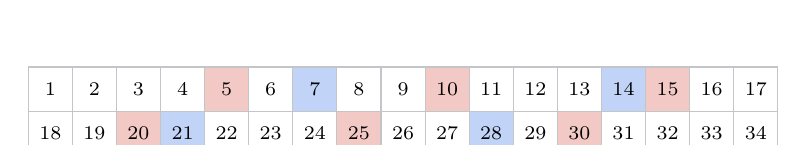
\begin{tikzpicture}[x=5.6mm,y=5.6mm]
  \foreach \k in {1,...,34}{
    \pgfmathtruncatemacro{\col}{mod(\k-1,17)}
    \pgfmathtruncatemacro{\row}{(\k-1)/17}
    \pgfmathtruncatemacro{\mf}{mod(\k,5)}
    \pgfmathtruncatemacro{\ms}{mod(\k,7)}
    \ifnum\mf=0 \fill[warn!30] (\col,-\row) rectangle ++(1,-1);\fi
    \ifnum\ms=0 \fill[acc!30] (\col,-\row) rectangle ++(1,-1);\fi
    \draw[gray!60] (\col,-\row) rectangle ++(1,-1);
    \node[font=\scriptsize] at (\col+0.5,-\row-0.5) {\k};
  }
\end{tikzpicture}\\[2pt]
{\footnotesize red = multiple of 5 (6 numbers), blue = multiple of 7 (4 numbers); $34 - 10 = 24$ white cells}
\end{center}

\begin{trap}[: repeated prime factors]
$25 = 5 \times 5$ is \textbf{not} a product of two distinct primes, so $(5-1)(5-1) = 16$ is wrong. Use rule 3: $\phi(25) = 25 - 5 = \mathbf{20}$. (Check: among $1, \dots, 24$ only 5, 10, 15, 20 share a factor with 25, leaving $24 - 4 = 20$.) The slides make the same point with $\phi(49)$: writing $\phi(49) = \phi(7)\phi(7) = 36$ is wrong because 7 and 7 are not co-prime; the correct value is $49 - 7 = 42$.
\end{trap}

\begin{worked}[: $\phi(n)$ from the factorisation (Forouzan / slide style)]
\textbf{Q.} Find (a) $\phi(29)$ (b) $\phi(32)$ (c) $\phi(80)$ (d) $\phi(100)$ (e) $\phi(101)$ (f) $\phi(240)$ (g) $\phi(1000)$ (h) $\phi(7000)$.

\textbf{A.} Factorise first, then apply the rules.
\begin{center}\small
\begin{tabular}{@{}llll@{}}
\toprule
$n$ & Factorisation & Working & $\phi(n)$\\
\midrule
29 & prime & $29 - 1$ & \textbf{28}\\
32 & $2^5$ & $2^5 - 2^4 = 32 - 16$ & \textbf{16}\\
80 & $2^4 \cdot 5$ & $(2^4 - 2^3)(5 - 1) = 8 \cdot 4$ & \textbf{32}\\
100 & $2^2 \cdot 5^2$ & $(4 - 2)(25 - 5) = 2 \cdot 20$ & \textbf{40}\\
101 & prime & $101 - 1$ & \textbf{100}\\
240 & $2^4 \cdot 3 \cdot 5$ & $(16 - 8)(3 - 1)(5 - 1) = 8 \cdot 2 \cdot 4$ & \textbf{64}\\
1000 & $2^3 \cdot 5^3$ & $1000 \cdot \frac12 \cdot \frac45$ \;(or $\phi(8)\phi(125) = 4 \cdot 100$) & \textbf{400}\\
7000 & $2^3 \cdot 5^3 \cdot 7$ & $7000 \cdot \frac12 \cdot \frac45 \cdot \frac67 = 7000 \cdot \frac{24}{70}$ & \textbf{2400}\\
\bottomrule
\end{tabular}
\end{center}
\textbf{Check:} a direct count of the co-prime $k < n$ by script gives the same eight values. Lecture homework: $\phi(369) = \phi(3^2)\phi(41) = 6 \cdot 40 = \mathbf{240}$ and $\phi(372) = \phi(2^2)\phi(3)\phi(31) = 2 \cdot 2 \cdot 30 = \mathbf{120}$.
\end{worked}

\textbf{$\phi(n)$ is even for every $n > 2$.} If $\gcd(k, n) = 1$ then also $\gcd(n - k, n) = 1$, so the co-prime numbers below $n$ come in pairs $\{k, n-k\}$. The two members of a pair can only coincide if $n = 2k$, but then $\gcd(k, n) = k$, which equals 1 only for $n = 2$. Hence for $n > 2$ the co-prime numbers split into disjoint pairs and their count is even; in $\mathbb{Z}_{14}^*$ the pairs are $\{1, 13\}$, $\{3, 11\}$, $\{5, 9\}$.

\subsection{The sets $\mathbb{Z}_n$ and $\mathbb{Z}_n^*$}
$\mathbb{Z}_n = \{0, 1, \dots, n-1\}$ is the set of residues modulo $n$. Every element has an additive inverse in it ($a + (n - a) \equiv 0$), but not every element has a multiplicative inverse. Since cryptosystems such as the affine cipher, Hill cipher and RSA need to \emph{divide}, they work in the smaller set
\[
\mathbb{Z}_n^* = \{\, a \in \mathbb{Z}_n : \gcd(a, n) = 1 \,\},
\]
which is exactly the set of residues that have multiplicative inverses. By definition its size is $|\mathbb{Z}_n^*| = \phi(n)$. The slide's rule of thumb: \imp{use $\mathbb{Z}_n$ when additive inverses are needed and $\mathbb{Z}_n^*$ when multiplicative inverses are needed.}

$\mathbb{Z}_n^*$ is closed under multiplication modulo $n$, because a product of two numbers co-prime to $n$ is again co-prime to $n$ (no prime factor of $n$ can appear in it). Together with the inverses this makes $\langle \mathbb{Z}_n^*, \times \rangle$ a group of order $\phi(n)$ (\S\ref{sec:algebra}), and the theorems of the next section are statements about this group. The slides single out the two sets with a \emph{prime} modulus, $\mathbb{Z}_p$ and $\mathbb{Z}_p^*$. When $n = p$ is prime, $\mathbb{Z}_p^* = \{1, 2, \dots, p-1\}$ contains every non-zero residue (e.g.\ $\mathbb{Z}_{13}^* = \{1, \dots, 12\}$), so every non-zero element of $\mathbb{Z}_p$ can be divided by, which is what makes $\mathbb{Z}_p$ the field GF$(p)$.
\begin{center}\small
\begin{tabular}{@{}lll@{}}
\toprule
$n$ & $\mathbb{Z}_n^*$ & $|\mathbb{Z}_n^*| = \phi(n)$\\
\midrule
6 & $\{1, 5\}$ & $\phi(2)\phi(3) = 2$\\
7 & $\{1, 2, 3, 4, 5, 6\}$ & $7 - 1 = 6$\\
10 & $\{1, 3, 7, 9\}$ & $\phi(2)\phi(5) = 4$\\
14 & $\{1, 3, 5, 9, 11, 13\}$ & $\phi(2)\phi(7) = 1 \cdot 6 = 6$ \;(slide Example 5)\\
21 & $\{1, 2, 4, 5, 8, 10, 11, 13, 16, 17, 19, 20\}$ & $\phi(3)\phi(7) = 2 \cdot 6 = 12$\\
26 & the 12 odd numbers except 13 & $\phi(2)\phi(13) = 12$ \;(valid keys/determinants mod 26)\\
\bottomrule
\end{tabular}
\end{center}

\subsection{Why cryptography cares about \texorpdfstring{$\phi(n)$}{phi(n)}}
Three later topics rest on $\phi(n)$. First, Euler's theorem (\S\ref{sec:fermat}) states that $a^{\phi(n)} \equiv 1 \pmod n$ for every $a \in \mathbb{Z}_n^*$, which allows exponents to be reduced modulo $\phi(n)$ and inverses to be computed as $a^{\phi(n)-1}$. Second, RSA chooses $n = pq$ and computes $\phi(n) = (p-1)(q-1)$; the keys satisfy $ed \equiv 1 \pmod{\phi(n)}$, and Euler's theorem then makes decryption undo encryption. In the standard example $n = 187 = 11 \cdot 17$, $\phi(187) = 160$ and $7 \cdot 23 = 161 \equiv 1 \pmod{160}$, which is why $88^7 \bmod 187 = 11$ and $11^{23} \bmod 187 = 88$ undo each other. Third, the number of primitive roots of a prime $p$ is $\phi(p - 1)$, which matters for Diffie--Hellman and ElGamal.

\textbf{Security.} Knowing $\phi(n)$ for an RSA modulus is equivalent to knowing its factors. From $n = pq$ and $\phi(n) = n - (p + q) + 1$ one gets $p + q = n - \phi(n) + 1$, and $p, q$ are then the roots of $z^2 - (p+q)z + n = 0$. For $n = 143$ and $\phi(n) = 120$: $p + q = 24$, $pq = 143$, so $p, q = \mathbf{11, 13}$. This is why $\phi(n)$ is part of the private key.

\begin{fixbox}
\begin{itemize}
  \item All values recomputed by script: $\phi(5) = 4$, $\phi(8) = 4$, $\phi(11) = 10$, $\phi(35) = 24$, $\phi(25) = 20$, $\phi(49) = 42$, $\phi(240) = 64$, $\phi(1000) = 400$, $\phi(7000) = 2400$, $|\mathbb{Z}_{14}^*| = 6$, $|\mathbb{Z}_{21}^*| = 12$. The homework answers in the old notes ($\phi(369) = 240$, $\phi(372) = 120$) are correct.
  \item Slide L10-06 gives $\phi(1) = 0$, which follows Forouzan's ``integers smaller than $n$'' wording. The standard convention is $\phi(1) = 1$ (count $1 \le k \le n$). It only affects $n = 1$ and never matters in RSA.
  \item The lecture video's ``case 3'' (``either or both numbers composite'') makes the product formula $n\prod(1 - 1/p)$ look like a last resort. It actually works for every $n$, and the prime and $pq$ formulas are special cases of it.
\end{itemize}
\end{fixbox}

% Lecture 10 (Fermat, Euler, inverses), Lecture 11 (order, primitive roots) + videos. All numbers recomputed by script (scratchpad/euler/v11.py).
\section{Fermat's and Euler's Theorems, Inverses and Primitive Roots}\label{sec:fermat}

Public-key cryptography computes powers $a^b \bmod n$ with exponents hundreds of digits long, and it needs inverses modulo $n$. Square-and-multiply (\S\ref{sec:modexp}) makes such powers feasible, but the two theorems of this section do more: they say that the powers of $a$ modulo $n$ repeat with a known period, so a huge exponent can be replaced by a small one, and they give a formula for the inverse. The same periodicity, studied element by element, leads to the order of an element and to primitive roots, which Diffie--Hellman and ElGamal are built on.

\subsection{Fermat's little theorem and exponent reduction \hot}
\asked{Mid-sem 2024--25 Q5(ii) (part of 3 marks): $100^{95} \bmod 9$, $658^{17} \bmod 17$, $145^{102} \bmod 101$.}
\textbf{First version.} \imp{If $p$ is prime and $a$ is an integer not divisible by $p$, then $a^{p-1} \equiv 1 \pmod p$.} Both conditions must be checked before the theorem is used: for a composite modulus or for $p \mid a$ it says nothing.

\textbf{Why it is true.} Multiply each of $1, 2, \dots, p-1$ by $a$ and reduce modulo $p$. No product is 0, because $p$ divides neither factor, and no two products are equal, because $ai \equiv aj$ would mean $p \mid a(i - j)$ and hence $p \mid (i - j)$, i.e.\ $i = j$. The $p - 1$ products are therefore just $1, \dots, p-1$ in a different order; for $p = 7$, $a = 3$ they are $3, 6, 2, 5, 1, 4$. Multiplying all of them together gives $a^{p-1}(p-1)! \equiv (p-1)! \pmod p$, and since $(p-1)!$ is co-prime to $p$ it can be cancelled, leaving $a^{p-1} \equiv 1$.

\textbf{Second version.} \imp{If $p$ is prime, then $a^p \equiv a \pmod p$ for every integer $a$.} This removes the condition on $a$. If $p \nmid a$, it is the first version multiplied by $a$; if $p \mid a$, both sides are $\equiv 0$.
\begin{center}\small
\begin{tabular}{@{}llll@{}}
\toprule
$p$, $a$ & Conditions & Working & Result\\
\midrule
5, 2 & prime, $5 \nmid 2$ & $2^4 = 16 = 3\cdot5 + 1$ & $\equiv 1$ \checkmark\\
13, 11 & prime, $13 \nmid 11$ & $11 \equiv -2$, $(-2)^{12} = \big((-2)^4\big)^3 = 16^3 \equiv 3^3 = 27 \equiv 1$ & $\equiv 1$ \checkmark\\
6, 2 & \textbf{6 not prime} & $2^5 = 32 = 5\cdot6 + 2$ & $\equiv 2 \ne 1$: theorem silent\\
11, 5 (homework) & prime, $11 \nmid 5$ & $5^2 \equiv 3$, $5^4 \equiv 9$, $5^8 \equiv 81 \equiv 4$, $5^{10} = 5^8 \cdot 5^2 \equiv 4 \cdot 3 = 12$ & $\equiv 1$ \checkmark\\
\bottomrule
\end{tabular}
\end{center}

\textbf{Exponent reduction.} Since $a^{p-1} \equiv 1$, the powers of $a$ modulo $p$ repeat with period dividing $p - 1$. Writing the exponent as $b = q(p-1) + r$ with $r = b \bmod (p-1)$ gives
\[
a^b = \left(a^{p-1}\right)^q a^r \equiv 1^q \cdot a^r = a^{\,b \bmod (p-1)} \pmod p \qquad (p \text{ prime},\ p \nmid a).
\]
The slides' examples follow directly: $6^{10} \bmod 11 = 1$ because the exponent is exactly $p - 1$, and $3^{12} \bmod 11 = 3^{11} \cdot 3 \equiv 3 \cdot 3 = 9$ by the second version (equivalently $12 \bmod 10 = 2$ and $3^2 = 9$). In practice the base is reduced modulo $p$ first, then the exponent modulo $p - 1$, and the small power that remains is computed by repeated squaring.

\begin{trap}[: what to reduce, and by what]
The \textbf{base} is reduced modulo $p$; the \textbf{exponent} is reduced modulo $p - 1$, never modulo $p$. And the modulus must be prime: in $100^{95} \bmod 9$ the modulus $9 = 3^2$ is composite, so Fermat does not apply. There the base reduction alone finishes the job ($100 \equiv 1 \pmod 9$), or Euler's theorem with $\phi(9) = 6$ can be used.
\end{trap}

\begin{worked}[: exponent reduction by Fermat (Forouzan exercise)]
\textbf{Q.} Using Fermat's little theorem, find (a) $5^{15} \bmod 13$ (b) $15^{18} \bmod 17$ (c) $456^{17} \bmod 17$.

\textbf{A.}
\begin{center}\small
\begin{tabular}{@{}lllll@{}}
\toprule
 & Conditions & Base & Exponent & Result\\
\midrule
(a) & 13 prime, $13 \nmid 5$ & 5 & $15 = 1\cdot12 + 3 \to 3$ & $5^3 = 125 = 9\cdot13 + 8 \Rightarrow \mathbf{8}$\\
(b) & 17 prime, $17 \nmid 15$ & $15 \equiv -2$ & $18 = 1\cdot16 + 2 \to 2$ & $(-2)^2 = \mathbf{4}$\\
(c) & 17 prime & $456 = 26\cdot17 + 14 \to 14$ & second version: $a^{17} \equiv a$ & $\mathbf{14}$\\
\bottomrule
\end{tabular}
\end{center}
\textbf{Check} (by script): $5^{15} \bmod 13 = 8$, $15^{18} \bmod 17 = 4$, $456^{17} \bmod 17 = 14$.
\end{worked}

\textbf{Fermat as a primality test.} Read backwards, the theorem gives a test: if $a^{n-1} \not\equiv 1 \pmod n$ for some $a$ with $\gcd(a, n) = 1$, then $n$ is certainly composite (e.g.\ $2^{14} \bmod 15 = 4$). The converse fails: $2^{340} \equiv 1 \pmod{341}$ although $341 = 11 \cdot 31$. The Fermat test, Carmichael numbers and Miller--Rabin are covered in \S\ref{sec:primes}.

\subsection{Euler's theorem \hot}
\asked{End-sem 2025--26 Q6(b): short note on Euler's theorem (2 marks).}
\likely{Exponent reduction modulo $\phi(n)$ for a composite $n$, and ``why does RSA decryption work?'' (Euler is its basis).}
Fermat's theorem needs a prime modulus, but RSA works modulo $n = pq$. Euler's theorem is the generalisation to any modulus. \textbf{First version:} \imp{if $\gcd(a, n) = 1$, then $a^{\phi(n)} \equiv 1 \pmod n$.} When $n = p$ is prime, $\phi(p) = p - 1$ and this is exactly Fermat's theorem.

\textbf{Why it is true.} The proof is the same permutation argument, run over $\mathbb{Z}_n^*$ (\S\ref{sec:totient}) instead of $\{1, \dots, p-1\}$. Multiplying the $\phi(n)$ elements of $\mathbb{Z}_n^*$ by $a$ permutes them, because $a$ is invertible; for $n = 10$, $a = 3$ the set $\{1, 3, 7, 9\}$ becomes $\{3, 9, 1, 7\}$. Taking the product of all elements on both sides gives $a^{\phi(n)} \cdot \Pi \equiv \Pi$, and the product $\Pi$ is invertible, so $a^{\phi(n)} \equiv 1$.

The co-prime condition is genuinely needed. If $\gcd(a, n) = d > 1$, every power of $a$ is a multiple of $d$, and so is every number $\equiv a^k \pmod n$; such a number can never be $\equiv 1$. The lecture homework $11^{20} \bmod 33$ shows this: the powers of 11 alternate $11, 22, 11, 22, \dots$, so $11^{20} \equiv 22 \ne 1$ although $\phi(33) = 20$.
\begin{center}\small
\begin{tabular}{@{}llll@{}}
\toprule
$a$, $n$ & $\gcd$ & Working & Result\\
\midrule
3, 10 & 1 & $\phi(10) = 4$; $3^4 = 81 = 8\cdot10 + 1$ & $\equiv 1$ \checkmark\\
2, 10 & \textbf{2} & $2^4 = 16 \equiv 6$ & $\ne 1$: theorem silent\\
10, 11 & 1 & $\phi(11) = 10$; $10 \equiv -1$, $(-1)^{10} = 1$ & $\equiv 1$ \checkmark\\
6, 35 & 1 & $\phi(35) = 24$; slide example $6^{24} \bmod 35$ & $\equiv 1$ \checkmark\\
11, 33 (homework) & \textbf{11} & $\phi(33) = 20$; powers alternate $11, 22$ & $11^{20} \equiv 22 \ne 1$\\
\bottomrule
\end{tabular}
\end{center}

\textbf{Exponent reduction.} Exactly as with Fermat, $\gcd(a, n) = 1$ and $b = q\phi(n) + r$ give $a^b \equiv a^{\,b \bmod \phi(n)} \pmod n$. The work is in computing $\phi(n)$, which needs the factorisation of $n$.

\textbf{Second version.} \imp{For $n = pq$ (and more generally any squarefree $n$), $a^{k\phi(n)+1} \equiv a \pmod n$ for every integer $a$ and every $k \ge 0$.} This removes the co-prime condition, which RSA needs because a message $M$ might, by bad luck, share the factor $p$ with $n$. The proof works one prime at a time. Modulo $p$: if $p \nmid a$, then $a^{k\phi(n)} = \big(a^{p-1}\big)^{k(q-1)} \equiv 1$ by Fermat, so $a^{k\phi(n)+1} \equiv a$; if $p \mid a$, both sides are $\equiv 0$. The same holds modulo $q$. Since the distinct primes $p$ and $q$ both divide $a^{k\phi(n)+1} - a$, so does $pq$. For example $11^{21} = 11^{\phi(33)+1} \equiv 11 \pmod{33}$ although $\gcd(11, 33) \ne 1$. The argument breaks when a prime appears squared: for $n = 4$, $a = 2$, $k = 1$ the claim would be $2^3 \equiv 2$, but $2^3 = 8 \equiv 0 \pmod 4$.

\textbf{Why RSA decryption works.} RSA picks $e$ and $d$ with $ed \equiv 1 \pmod{\phi(n)}$, i.e.\ $ed = k\phi(n) + 1$. Decrypting $C = M^e$ gives $C^d = M^{ed} = M^{k\phi(n)+1} \equiv M \pmod n$ by the second version, for every message $M < n$. In the example $n = 187$, $e = 7$, $d = 23$: $ed = 161 = 1 \cdot 160 + 1$, and indeed $88^7 \bmod 187 = 11$ and $11^{23} \bmod 187 = 88$.

\begin{mustknow}
\begin{center}\small
\begin{tabular}{@{}lll@{}}
\toprule
 & First version & Second version (no co-prime condition)\\
\midrule
Fermat ($p$ prime) & $a^{p-1} \equiv 1 \pmod p$ if $p \nmid a$ & $a^p \equiv a \pmod p$\\
Euler & $a^{\phi(n)} \equiv 1 \pmod n$ if $\gcd(a,n) = 1$ & $a^{k\phi(n)+1} \equiv a \pmod n$ ($n = pq$, squarefree)\\
\midrule
Reduction & \multicolumn{2}{l}{$a^b \equiv a^{\,b \bmod (p-1)} \pmod p$ \quad and \quad $a^b \equiv a^{\,b \bmod \phi(n)} \pmod n$ \quad (co-prime $a$)}\\
Inverse & \multicolumn{2}{l}{$a^{-1} \equiv a^{p-2} \pmod p$ \quad and \quad $a^{-1} \equiv a^{\phi(n)-1} \pmod n$ \quad (co-prime $a$)}\\
\bottomrule
\end{tabular}
\end{center}
\end{mustknow}

\begin{worked}[: exponent reduction by Euler]
\textbf{Q.} Using Euler's theorem, find (a) $11^{2024} \bmod 35$ (b) the last two digits of $3^{1003}$ (c) $20^{62} \bmod 77$ (slide example).

\textbf{A.}
\begin{center}\small
\begin{tabular}{@{}lllll@{}}
\toprule
 & $\gcd$, $\phi(n)$ & Exponent & Remaining power & Result\\
\midrule
(a) & $\gcd(11, 35) = 1$, $\phi(35) = 4 \cdot 6 = 24$ & $2024 = 84\cdot24 + 8$ & $11^2 = 121 \equiv 16$, $11^4 \equiv 16^2 = 256 \equiv 11$, $11^8 \equiv 11^2 \equiv 16$ & $\mathbf{16}$\\
(b) & $\gcd(3, 100) = 1$, $\phi(100) = 40$ & $1003 = 25\cdot40 + 3$ & $3^3 = 27$ & $\mathbf{27}$\\
(c) & $\gcd(20, 77) = 1$, $\phi(77) = 6 \cdot 10 = 60$ & $62 = 1\cdot60 + 2$ & $20^2 = 400 = 5\cdot77 + 15$ & $\mathbf{15}$\\
\bottomrule
\end{tabular}
\end{center}
For (b), ``last two digits'' means the residue modulo 100. \textbf{Check} (by script): $11^{2024} \bmod 35 = 16$, $3^{1003} \bmod 100 = 27$, $20^{62} \bmod 77 = 15$.
\end{worked}

\subsection{Multiplicative inverses via Fermat and Euler \hot}
\asked{Mid-sem 2024--25 Q5(iii): $7^{-1} \bmod 17$, $15^{-1} \bmod 99$ (does not exist).}
The multiplicative inverse of $a$ modulo $n$ is the residue $a^{-1}$ with \imp{$a \cdot a^{-1} \equiv 1 \pmod n$; it exists if and only if $\gcd(a, n) = 1$} (derived in \S\ref{sec:totient}). It depends on the modulus as well as on $a$: $2^{-1}$ is 3 modulo 5 but 4 modulo 7. For small $n$ it can be found by trial, multiplying $a$ by $1, 2, 3, \dots$ until the product is $\equiv 1$:
\begin{center}\small
\begin{tabular}{@{}lllll@{}}
\toprule
$a \bmod n$ & $\gcd$ & Search & Inverse & Note\\
\midrule
$3 \bmod 5$ & 1 & $3\cdot2 = 6 \equiv 1$ & \textbf{2} & so $2^{-1} \bmod 5 = 3$ as well\\
$2 \bmod 11$ & 1 & $2\cdot6 = 12 \equiv 1$ & \textbf{6} & \\
$4 \bmod 5$ & 1 & $4\cdot4 = 16 \equiv 1$ & \textbf{4} & its own inverse ($4 \equiv -1$)\\
$2 \bmod 7$ & 1 & $2\cdot4 = 8 \equiv 1$ & \textbf{4} & not 3: depends on $n$\\
$5 \bmod 10$ & \textbf{5} & $5k \bmod 10 \in \{0, 5\}$ only & \textbf{none} & \\
\bottomrule
\end{tabular}
\end{center}

\textbf{Inverse by exponentiation.} Fermat's theorem already contains the inverse. If $p$ is prime and $p \nmid a$, then $a \cdot a^{p-2} = a^{p-1} \equiv 1$, so
\[
a^{-1} \equiv a^{p-2} \pmod p, \qquad\text{and in the same way}\qquad a^{-1} \equiv a^{\phi(n)-1} \pmod n \ \text{ if } \gcd(a, n) = 1.
\]
This replaces the extended Euclidean algorithm by one modular exponentiation, which is convenient when the modulus is prime or when $\phi(n)$ is known. The price is that for a composite $n$ the factorisation is needed to get $\phi(n)$. The slides' examples (L10-15 and L10-20), all checked by script:
\begin{center}\small
\begin{tabular}{@{}ll@{\qquad}lll@{}}
\toprule
\multicolumn{2}{@{}l}{Fermat ($n$ prime)} & \multicolumn{3}{l}{Euler ($n$ composite)}\\
\midrule
$8^{-1} \bmod 17 = 8^{15}$ & $= 15$ & $8^{-1} \bmod 77 = 8^{59}$ & $= 29$ & $\phi(77) = 60$\\
$5^{-1} \bmod 23 = 5^{21}$ & $= 14$ & $7^{-1} \bmod 15 = 7^{7}$ & $= 13$ & $\phi(15) = 8$\\
$60^{-1} \bmod 101 = 60^{99}$ & $= 32$ & $60^{-1} \bmod 187 = 60^{159}$ & $= 53$ & $\phi(187) = 160$\\
$22^{-1} \bmod 211 = 22^{209}$ & $= 48$ & $71^{-1} \bmod 100 = 71^{39}$ & $= 31$ & $\phi(100) = 40$\\
$2^{-1} \bmod 13 = 2^{11}$ & $= 7$ & $3^{-1} \bmod 20 = 3^{7}$ & $= 7$ & $\phi(20) = 8$\\
\bottomrule
\end{tabular}
\end{center}
Each answer is checked by one multiplication, e.g.\ $8 \cdot 15 = 120 = 7\cdot17 + 1$ and $7 \cdot 13 = 91 = 6\cdot15 + 1$.

\begin{trap}[: the inverse may not exist]
Before using any formula, compute $\gcd(a, n)$. If it is not 1 there is no inverse, and the exam expects exactly that answer with the reason. Blindly applying Euler's formula still produces a number, which is wrong: for $15^{-1} \bmod 99$, $\phi(99) = 60$ and $15^{59} \bmod 99 = 36$, but $15 \cdot 36 = 540 \equiv 45 \not\equiv 1 \pmod{99}$.
\end{trap}

\begin{worked}[: 2024--25 Q5(ii) and (iii), as it should be written]
\textbf{Q.} (ii) Find the values of $100^{95} \bmod 9$, $658^{17} \bmod 17$ and $145^{102} \bmod 101$. (iii) Find the values of $7^{-1} \bmod 17$ and $15^{-1} \bmod 99$.

\textbf{A.} (ii) \textbf{$100^{95} \bmod 9$.} The modulus 9 is not prime, so Fermat's theorem cannot be used; reduce the base instead. $100 = 11 \cdot 9 + 1$, so $100 \equiv 1 \pmod 9$ and $100^{95} \equiv 1^{95} = \mathbf{1}$. (Euler agrees: $\gcd(100, 9) = 1$, $\phi(9) = 6$, $95 \bmod 6 = 5$, $1^5 = 1$.)

\textbf{$658^{17} \bmod 17$.} 17 is prime, so by the second version of Fermat's theorem $a^{17} \equiv a \pmod{17}$. $658 = 38 \cdot 17 + 12$, hence $658^{17} \equiv 658 \equiv \mathbf{12}$.

\textbf{$145^{102} \bmod 101$.} 101 is prime and $101 \nmid 145$. Base: $145 \equiv 44$. Exponent: $102 = 1 \cdot 100 + 2$, and $44^{100} \equiv 1$ by Fermat. So $145^{102} \equiv 44^2 = 1936 = 19 \cdot 101 + 17$, i.e.\ $\mathbf{17}$.

(iii) \textbf{$7^{-1} \bmod 17$.} 17 is prime and $17 \nmid 7$, so $7^{-1} \equiv 7^{17-2} = 7^{15} \pmod{17}$. With $15 = 8 + 4 + 2 + 1$:
\begin{center}\small
\begin{tabular}{@{}lllll@{}}
\toprule
$7^1$ & $7^2$ & $7^4$ & $7^8$ & $7^{15} = 7^8 \cdot 7^4 \cdot 7^2 \cdot 7$\\
\midrule
7 & $49 \equiv 15$ & $15^2 = 225 \equiv 4$ & $4^2 = 16$ & $16 \cdot 4 = 64 \equiv 13$;\; $13 \cdot 15 = 195 \equiv 8$;\; $8 \cdot 7 = 56 \equiv \mathbf{5}$\\
\bottomrule
\end{tabular}
\end{center}
So $7^{-1} \bmod 17 = \mathbf{5}$. Check: $7 \cdot 5 = 35 = 2 \cdot 17 + 1$ \checkmark.

\textbf{$15^{-1} \bmod 99$.} $\gcd(99, 15)$: $99 = 6 \cdot 15 + 9$, $15 = 1 \cdot 9 + 6$, $9 = 1 \cdot 6 + 3$, $6 = 2 \cdot 3 + 0$, so $\gcd = 3 \ne 1$. Every number $15x - 99k$ is a multiple of 3 and can never equal 1, therefore \textbf{$15^{-1} \bmod 99$ does not exist}.
\end{worked}

\textbf{Which method?} All four methods give the same inverse when it exists; they differ in what they need. The summary below is the decision to make in an exam.
\begin{center}\small
\begin{tabularx}{\textwidth}{@{}l l X@{}}
\toprule
Method & Formula & When to use\\
\midrule
Trial & $a\cdot1, a\cdot2, \dots$ until $\equiv 1$ & Small $n$ only (mod 26 ciphers, GF(7) division).\\
Fermat & $a^{-1} = a^{p-2} \bmod p$ & Prime modulus; compute with square-and-multiply.\\
Euler & $a^{-1} = a^{\phi(n)-1} \bmod n$ & Composite $n$ whose factorisation (hence $\phi(n)$) is known.\\
\textbf{Extended Euclid} & $sa + tn = 1 \Rightarrow a^{-1} = s \bmod n$ & The general method: works for any $n$ without factoring, and detects ``no inverse'' (final $\gcd \ne 1$). The past papers ask for it explicitly (2024--25 Q7, \S\ref{sec:exteuclid}); RSA uses it to find $d$.\\
\bottomrule
\end{tabularx}
\end{center}

\subsection{Order of an element \new}
\likely{``Find the order of every element of $\mathbb{Z}_7^*$ / $\mathbb{Z}_{10}^*$'' (Forouzan), usually as the first step of a primitive-root question.}
Euler's theorem says that $a^{\phi(n)} \equiv 1$ for every $a \in \mathbb{Z}_n^*$, but many elements return to 1 much earlier. \imp{The order of $a$ modulo $n$, $\operatorname{ord}(a)$, is the smallest positive integer $i$ with $a^i \equiv 1 \pmod n$.} It exists for every $a \in \mathbb{Z}_n^*$, and Euler's theorem guarantees $\operatorname{ord}(a) \le \phi(n)$. After $a^{\operatorname{ord}(a)} = 1$ the powers start over, so the sequence $a, a^2, a^3, \dots$ is periodic with period exactly $\operatorname{ord}(a)$.

\textbf{The key property: $a^m \equiv 1 \iff \operatorname{ord}(a) \mid m$.} Write $m = q \cdot \operatorname{ord}(a) + r$ with $0 \le r < \operatorname{ord}(a)$. Then $a^m = \big(a^{\operatorname{ord}(a)}\big)^q a^r \equiv a^r$, and by the minimality of the order $a^r \equiv 1$ only for $r = 0$. Two consequences follow. First, since $a^{\phi(n)} \equiv 1$, \textbf{the order always divides $\phi(n)$} (this is Lagrange's theorem for the group $\mathbb{Z}_n^*$), so to find an order only the divisors of $\phi(n)$ need to be tried. Second, exponents can be reduced modulo $\operatorname{ord}(a)$, which is sharper than reducing modulo $\phi(n)$: $\operatorname{ord}(2) = 3$ modulo 7, so $2^{100} \equiv 2^{100 \bmod 3} = 2^1 = 2 \pmod 7$.

The table lists $a^i \bmod 7$ for the whole group $\mathbb{Z}_7^*$ (slide L11-30); the shaded cell is the first 1 in each row, and its column is the order. Every order is a divisor of $\phi(7) = 6$, and only $a = 3$ and $a = 5$ reach the maximum 6.
\begin{center}\small
\begin{tabular}{@{}c|cccccc|c@{}}
\toprule
$a$ & $i=1$ & 2 & 3 & 4 & 5 & 6 & $\operatorname{ord}(a)$\\
\midrule
1 & \hl{1} & 1 & 1 & 1 & 1 & 1 & 1\\
2 & 2 & 4 & \hl{1} & 2 & 4 & 1 & 3\\
3 & 3 & 2 & 6 & 4 & 5 & \hl{1} & \textbf{6}\\
4 & 4 & 2 & \hl{1} & 4 & 2 & 1 & 3\\
5 & 5 & 4 & 6 & 2 & 3 & \hl{1} & \textbf{6}\\
6 & 6 & \hl{1} & 6 & 1 & 6 & 1 & 2\\
\bottomrule
\end{tabular}
\end{center}
Two more slide examples (L11-27, L11-29): in $\mathbb{Z}_{10}^* = \{1, 3, 7, 9\}$ the orders are $1, 4, 4, 2$ ($3^2 = 9$, $3^4 = 81 \equiv 1$), and in $\mathbb{Z}_8^* = \{1, 3, 5, 7\}$ they are $1, 2, 2, 2$, because $3^2 = 9$, $5^2 = 25$ and $7^2 = 49$ are all $\equiv 1 \pmod 8$.

\subsection{Primitive roots \hot}
\asked{End-sem 2025--26 Q2(a)(i): find the primitive roots of GF(19) (they are 2, 3, 10, 13, 14, 15).}
\likely{``Find all primitive roots of 7 / 11 / 13'', ``is 3 a primitive root of 17?'', ``how many primitive roots does 17 have?'' (needed for Diffie--Hellman and ElGamal).}

\textbf{The idea, for a prime $p$.} Take the multiplicative group $\mathbb{Z}_p^* = \{1, 2, \dots, p-1\}$, which is $\mathbb{Z}_p$ without 0. Pick an element $g$ and write down its powers $g^1, g^2, g^3, \dots \pmod p$. Two things can happen. Either the powers run through \emph{every} element of $\mathbb{Z}_p^*$ before returning to 1, or they hit 1 early and then repeat a smaller cycle. In the first case \imp{$g$ is called a primitive root of $p$: its powers $g^1, \dots, g^{p-1}$ produce each of $1, \dots, p-1$ exactly once.} Modulo 7, for example:
\begin{center}\small
\begin{tabular}{@{}lccccccl@{}}
\toprule
 & $g^1$ & $g^2$ & $g^3$ & $g^4$ & $g^5$ & $g^6$ & \\
\midrule
$g = 3$ & 3 & 2 & 6 & 4 & 5 & 1 & all six elements: \textbf{primitive root}\\
$g = 2$ & 2 & 4 & 1 & 2 & 4 & 1 & only $\{2, 4, 1\}$: \textbf{not} a primitive root\\
\bottomrule
\end{tabular}
\end{center}
Since the powers start repeating as soon as they reach 1, the number of different powers equals the order of $g$. Producing all $p - 1$ elements therefore means exactly that \textbf{$\operatorname{ord}(g) = p - 1$}, the largest order possible. When such a $g$ exists, every element of the group is a power of it, so the group is \emph{cyclic} and $g$ is a \emph{generator}. Every element $y$ is then $g^x$ for exactly one $x \in \{1, \dots, p-1\}$, and that $x$ is the discrete logarithm of $y$ (\S\ref{sec:primes}).

\textbf{Why cryptography needs them.} Diffie--Hellman and ElGamal publish $p$ and a base $g$, keep an exponent $x$ secret, and publish $g^x \bmod p$. If $g$ had a small order $d$, then $g^x$ could take only $d$ different values, and Eve could find a matching exponent by trying $d$ values. Choosing a primitive root makes all $p - 1$ values possible, so the search is as large as it can be.

\textbf{The same idea for any $n$.} Nothing changes except the group. For a general $n$ the group is $\mathbb{Z}_n^*$, the numbers below $n$ that are coprime to $n$, and it has $\phi(n)$ elements instead of $p - 1$. So \imp{$g \in \mathbb{Z}_n^*$ is a primitive root of $n$ if $\operatorname{ord}(g) = \phi(n)$}, which means $g^1, \dots, g^{\phi(n)}$ produce every element of $\mathbb{Z}_n^*$ once each. Modulo 10, $\mathbb{Z}_{10}^* = \{1, 3, 7, 9\}$ and the powers of 3 are $3, 9, 7, 1$, so 3 is a primitive root of 10. The powers never produce 0, 2, 4, 5, 6 or 8, and they are not supposed to: a power of a number coprime to $n$ is itself coprime to $n$, so only $\mathbb{Z}_n^*$ can ever be generated, never all of $\mathbb{Z}_n$. For a prime this is the same statement as before, since $\mathbb{Z}_p^*$ is $\mathbb{Z}_p$ without 0 and $\phi(p) = p - 1$.

Unlike primes, many composite $n$ have \emph{no} primitive root at all, because every element returns to 1 too early. Modulo 8, the group $\mathbb{Z}_8^* = \{1, 3, 5, 7\}$ has $\phi(8) = 4$ elements, but $3^2$, $5^2$ and $7^2$ are all $\equiv 1$, so no order reaches 4 (slide L11-28). Modulo 15, every element satisfies $a^4 \equiv 1$, because $a^2 \equiv 1 \pmod 3$ and $a^4 \equiv 1 \pmod 5$, so no order reaches $\phi(15) = 8$. The complete answer is a theorem worth memorising:

\begin{mustknow}[: primitive roots]
$g$ is a primitive root of $n$ $\iff$ $\operatorname{ord}(g) = \phi(n)$ $\iff$ the powers of $g$ produce all of $\mathbb{Z}_n^*$ (for a prime: all of $1, \dots, p-1$).\\
Primitive roots exist \textbf{only} for $n = 2,\ 4,\ p^k,\ 2p^k$ ($p$ an odd prime). Every prime has them; 9, 10, 18 have them; 8, 12, 15 do not.\\
When they exist there are exactly $\phi(\phi(n))$ of them; for a prime $p$ that is $\phi(p-1)$.
\end{mustknow}

\textbf{Test 1: list the powers.} Multiply by $g$ repeatedly, reducing each time; for example $3^4 \equiv 6 \cdot 3 = 18 \equiv 4 \pmod 7$, so you never need $3^6 = 729$. If a 1 appears before the $(p-1)$-th power, stop: $g$ is not a primitive root.
\begin{center}\small
\begin{tabular}{@{}lll@{}}
\toprule
Test & Powers $g^1, g^2, \dots \pmod p$ & Verdict\\
\midrule
2 mod 5 & 2, 4, 3, 1 & order 4 $= p - 1$: \textbf{yes}\\
3 mod 5 & 3, 4, 2, 1 & \textbf{yes}\\
4 mod 5 & 4, \textbf{1} & order 2: no\\
3 mod 7 & 3, 2, 6, 4, 5, 1 & \textbf{yes}\\
2 mod 7 & 2, 4, \textbf{1} & order 3: no\\
2 mod 11 (homework) & 2, 4, 8, 5, 10, 9, 7, 3, 6, 1 & \textbf{yes}\\
\bottomrule
\end{tabular}
\end{center}
The homework ``primitive roots of 5'' is answered by the first three rows: 1 never works ($1^k = 1$), 2 and 3 do, and 4 does not, so the primitive roots of 5 are \textbf{2 and 3}.

\textbf{Test 2: the fast test.} Listing takes up to $p - 1$ multiplications. It is faster to use the fact that the order of $g$ must divide $p - 1$: if $g$ is not a primitive root, its order is a proper divisor of $p - 1$, and every proper divisor divides $(p-1)/q$ for some prime factor $q$ of $p - 1$. So it is enough to check those few exponents:
\begin{center}
\imp{$g$ is a primitive root of $p$ $\iff$ $g^{(p-1)/q} \not\equiv 1 \pmod p$ for every prime $q$ dividing $p - 1$.}
\end{center}
For $p = 7$, $p - 1 = 6 = 2 \cdot 3$, so check $g^3$ and $g^2$. For $g = 3$: $3^3 = 27 \equiv 6$ and $3^2 = 9 \equiv 2$, neither is 1, so 3 is a primitive root. For $g = 2$: $2^3 = 8 \equiv 1$, so 2 is not.

\textbf{Finding all of them from one.} Once one primitive root $g$ is known, the others are the powers $g^k$ with $\gcd(k, p-1) = 1$. The reason is that $g^k$ has order $\frac{p-1}{\gcd(k,\,p-1)}$, which equals $p - 1$ exactly when the gcd is 1. Counting those $k$ gives the $\phi(p-1)$ from the box: 5 has $\phi(4) = 2$ (2, 3), 7 has $\phi(6) = 2$ (3, 5), 11 has $\phi(10) = 4$ (2, 6, 7, 8), and 13 has $\phi(12) = 4$ (2, 6, 7, 11).

\begin{worked}[: all primitive roots of a prime]
\textbf{Q.} Find all the primitive roots of 11 (i.e.\ of the group $G = \langle \mathbb{Z}_{11}^*, \times \rangle$).

\textbf{A.} $\phi(11) = 10 = 2 \cdot 5$, so a primitive root $g$ must satisfy $g^{10/2} = g^5 \not\equiv 1$ and $g^{10/5} = g^2 \not\equiv 1$. Try $g = 2$: $2^2 = 4 \ne 1$ and $2^5 = 32 = 2\cdot11 + 10 \equiv 10 \ne 1$, so \textbf{2 is a primitive root}. (For contrast, $g = 3$ fails: $3^5 = 243 = 22 \cdot 11 + 1 \equiv 1$.)

The other primitive roots are $2^k$ with $\gcd(k, 10) = 1$, i.e.\ $k \in \{1, 3, 7, 9\}$:
\begin{center}\small
\begin{tabular}{@{}lcccc@{}}
\toprule
$k$ & 1 & 3 & 7 & 9\\
$2^k \bmod 11$ & 2 & 8 & $128 = 11\cdot11 + 7 \to 7$ & $512 = 46\cdot11 + 6 \to 6$\\
\bottomrule
\end{tabular}
\end{center}
The primitive roots of 11 are \textbf{2, 6, 7, 8}. \textbf{Check:} their number is $\phi(10) = 4$ \checkmark, and the full list of powers of 2 is $2, 4, 8, 5, 10, 9, 7, 3, 6, 1$, all ten residues.
\end{worked}

\begin{worked}[: fast test and counting]
\textbf{Q.} Show that 3 is a primitive root of 17 but 2 is not. How many primitive roots does 17 have? List them.

\textbf{A.} $\phi(17) = 16 = 2^4$, whose only prime factor is 2, so $g$ is a primitive root iff $g^{16/2} = g^8 \not\equiv 1 \pmod{17}$.
For $g = 3$: $3^2 = 9$, $3^4 = 81 \equiv 13$, $3^8 \equiv 13^2 = 169 \equiv 16 \ne 1$, so \textbf{3 is a primitive root}.
For $g = 2$: $2^4 = 16$, $2^8 \equiv 16^2 = 256 = 15\cdot17 + 1 \equiv 1$, so \textbf{2 is not} (its order is 8).
The number of primitive roots is $\phi(16) = \mathbf{8}$. They are $3^k$ for odd $k$: $3^1, 3^3, \dots, 3^{15} \equiv 3, 10, 5, 11, 14, 7, 12, 6$, i.e.\ \textbf{3, 5, 6, 7, 10, 11, 12, 14}.
\end{worked}

\begin{fixbox}
\begin{itemize}
  \item All values recomputed by script. The slides' inverse examples (L10-15: 15, 14, 32, 48; L10-20: 29, 13, 53, 31) and examples $6^{10} \bmod 11 = 1$, $3^{12} \bmod 11 = 9$, $6^{24} \bmod 35 = 1$, $20^{62} \bmod 77 = 15$ are correct. The video homework answers are correct: $5^{10} \equiv 1 \pmod{11}$, $11^{20} \equiv 22 \pmod{33}$, 2 is a primitive root of 11, the primitive roots of 5 are 2 and 3.
  \item Slide L10-16 says the second version of Euler's theorem ``removes the condition that $a$ and $n$ should be coprime''. That is true only for squarefree $n$ (such as $n = pq$ in RSA). It fails for $n = 4$, $a = 2$: $2^{\phi(4)+1} = 2^3 = 8 \equiv 0 \not\equiv 2$.
  \item Slide L10-18 solves $20^{62} \bmod 77$ with the second version, but $\gcd(20, 77) = 1$, so the first version already gives $20^{62} = 20^{60} \cdot 20^2 \equiv 400 \equiv 15$.
  \item Video notation: ``$-2^{12}$'' and ``$-1^{10}$'' mean $(-2)^{12}$ and $(-1)^{10}$. Without brackets $-2^{12} = -(2^{12})$; write the brackets in the exam.
  \item The general definition of a primitive root (any $n$) was stated in the video but not explained: only $n = 2, 4, p^k, 2p^k$ have primitive roots, and then there are $\phi(\phi(n))$ of them.
\end{itemize}
\end{fixbox}

% College Lectures 10-11: primes, primality tests, factorization, CRT, fast exponentiation, discrete logs.
% Every number in this file was recomputed by script (scratchpad/primes/verify*.py).
% Fermat/Euler second versions, inverses by Fermat/Euler, order and primitive roots now live in 11_fermat_euler.tex (sec:fermat).
\section{Primes, Primality Testing, Factorization, CRT and Discrete Logs}\label{sec:primes}

Asymmetric-key cryptography is built on a handful of facts about primes, and this chapter collects them. RSA needs two large random primes, so we need a fast way to decide whether a 1024-bit number is prime; this is \emph{primality testing}. RSA is secure only because nobody can split $n = pq$ back into $p$ and $q$; this is the hardness of \emph{factorization}. RSA decryption is made about four times faster by working modulo $p$ and $q$ separately and gluing the results with the \emph{Chinese remainder theorem}. Every public-key operation is a modular power, computed by \emph{square-and-multiply}. Finally, Diffie--Hellman and ElGamal rely on the fact that undoing a modular power, the \emph{discrete logarithm}, is infeasible.

\subsection{Primes and how many there are}
A positive integer is \imp{prime if it has exactly two divisors, 1 and itself}; a \emph{composite} has more than two divisors, and the number 1 (exactly one divisor) is neither. Two integers are \emph{coprime} (relatively prime) when their gcd is 1, so a prime $p$ is coprime to every integer from 1 to $p - 1$, which is why $\mathbb{Z}_p^* = \{1, \dots, p - 1\}$.

\textbf{Infinitely many primes.} Suppose the primes were only $p_1, \dots, p_k$, and let $N = p_1 p_2 \cdots p_k + 1$. Dividing $N$ by any $p_i$ leaves remainder 1, so $N$ either is a new prime or has a prime factor outside the list; either way the list was incomplete. Note that $N$ itself need not be prime: $2 \cdot 3 \cdot 5 \cdot 7 \cdot 11 \cdot 13 + 1 = 30031 = 59 \times 509$, but 59 and 509 are new primes.

\textbf{Counting primes.} The function $\pi(n)$ counts the primes $\le n$: $\pi(1) = 0$, $\pi(2) = 1$, $\pi(3) = 2$, $\pi(10) = 4$, $\pi(20) = 8$, $\pi(50) = 15$, $\pi(100) = 25$. For large $n$ there is no formula, only bounds (Lagrange found the lower one, Gauss the upper):
\[
\frac{n}{\ln n} \;<\; \pi(n) \;<\; \frac{n}{\ln n - 1.08366}.
\]
For $n = 10^6$: $n/\ln n = 72{,}382.4$ and $n/(\ln n - 1.08366) = 78{,}543.2$, so $72{,}383 \le \pi(10^6) \le 78{,}543$; the actual count is $78{,}498$. The practical consequence is that primes thin out only slowly: near $N$ about one number in $\ln N$ is prime. For 1024-bit numbers $\ln 2^{1024} \approx 710$, so if we test random \emph{odd} 1024-bit numbers, about one in 355 is prime, and generating an RSA prime takes a few hundred primality tests. This is why the test itself must be fast.

\textbf{Checking a number by $\sqrt n$.} If $n = ab$ with $1 < a \le b$, then $a^2 \le ab = n$, so $a \le \sqrt n$. Therefore a composite $n$ always has a prime factor $\le \lfloor \sqrt n \rfloor$, and it is enough to try the primes up to $\lfloor\sqrt n\rfloor$.
\begin{itemize}
  \item Is 97 prime? $\lfloor\sqrt{97}\rfloor = 9$, and none of 2, 3, 5, 7 divides 97, so \textbf{97 is prime}.
  \item Is 301 prime? $\lfloor\sqrt{301}\rfloor = 17$, so we would try 2, 3, 5, 7, 11, 13, 17; but already $7 \mid 301$ ($301 = 7 \times 43$), so \textbf{301 is composite}.
\end{itemize}

\textbf{Mersenne and Fermat numbers.} These were early attempts at formulas that produce primes. A \emph{Mersenne number} is $M_p = 2^p - 1$. If the exponent factors as $ab$, then $2^a - 1$ divides $2^{ab} - 1$ (since $x - 1 \mid x^b - 1$ with $x = 2^a$), so $M_p$ can be prime only for prime $p$. The condition is not sufficient: $M_2, M_3, M_5, M_7, M_{13}, M_{17}, M_{19} = 3, 7, 31, 127, 8191, 131071, 524287$ are prime, but $M_{11} = 2047 = 23 \times 89$ and $M_{23} = 8388607 = 47 \times 178481$. A \emph{Fermat number} is $F_n = 2^{2^n} + 1$. Fermat saw that $F_0, \dots, F_4 = 3, 5, 17, 257, 65537$ are prime and guessed that all are, but Euler found $F_5 = 4294967297 = 641 \times 6700417$, and no larger Fermat number is known to be prime. $F_4 = 65537 = 2^{16} + 1$ survives in practice as the standard RSA public exponent, because its binary form has only two 1-bits, which makes encryption with square-and-multiply cheap.

\subsection{Primality testing: deterministic and probabilistic}
The problem is to decide, for a number of several hundred digits, whether it is prime. A \emph{deterministic} algorithm always gives the correct answer; a \emph{probabilistic} algorithm is much faster but may declare a composite number ``prime'' with a small, controllable probability. Its ``composite'' answers are always correct, because they come with a witness.

\textbf{Divisibility test (deterministic).} Try every $r = 2, 3, \dots, \lfloor\sqrt n\rfloor$ and return ``composite'' as soon as $r \mid n$, otherwise ``prime''. It is correct by the $\sqrt n$ argument above, but its cost is exponential in the size of the input: an $n_b$-bit number has $\sqrt n \approx 2^{n_b/2}$ candidate divisors. For a 200-bit $n$ this is $2^{100}$ bit operations; at $2^{30}$ operations per second that takes $2^{70}$ seconds, about $3.7 \times 10^{13}$ years.

\textbf{AKS (deterministic, polynomial).} In 2002 Agrawal, Kayal and Saxena gave the first deterministic test whose time is polynomial in the number of bits, $O((\log_2 n)^{12})$ bit operations, based on the identity $(x - a)^p \equiv x^p - a \pmod p$, which holds exactly when $p$ is prime. It settled a theoretical question, but in practice the probabilistic tests below are far faster.

\textbf{Fermat test (probabilistic).} Fermat's little theorem says that if $n$ is prime then $a^{n-1} \equiv 1 \pmod n$ for every $a$ with $n \nmid a$. Read in reverse: \imp{if $a^{n-1} \not\equiv 1 \pmod n$, then $n$ is certainly composite}; if $a^{n-1} \equiv 1$, then $n$ is only \emph{probably} prime, because some composites also satisfy it. For example $341 = 11 \times 31$ gives $2^{340} \equiv 1 \pmod{341}$ (since $2^{10} = 1024 = 3 \cdot 341 + 1$), so base 2 is fooled, but base 3 exposes it: $3^{340} \equiv 56 \pmod{341}$.

\textbf{Carmichael numbers.} Trying more bases does not always help. A \emph{Carmichael number} is a composite $n$ with $a^{n-1} \equiv 1 \pmod n$ for \emph{every} $a$ coprime to $n$, so the Fermat test fails for all such bases. The smallest is $561 = 3 \times 11 \times 17$ (then 1105, 1729, 2465, 2821). The reason is visible from the factors: $561 - 1 = 560$ is divisible by $3 - 1$, $11 - 1$ and $17 - 1$, so for each prime factor $p$, $a^{560} = (a^{p-1})^{560/(p-1)} \equiv 1 \pmod p$, and a number that is $\equiv 1$ modulo 3, 11 and 17 is $\equiv 1$ modulo 561 (by the CRT below). In general $n$ is Carmichael exactly when it is squarefree and $(p - 1) \mid (n - 1)$ for every prime $p \mid n$ (Korselt's criterion). Only bases sharing a factor with $n$ catch it, e.g.\ $3^{560} \equiv 375 \pmod{561}$, and for large $n$ such bases are too rare to find by chance.

\textbf{Square-root test.} If $n = p$ is prime and $x^2 \equiv 1 \pmod p$, then $p \mid (x - 1)(x + 1)$, and since $p$ is prime it divides one of the two factors, so $x \equiv \pm 1 \pmod p$. Hence \imp{modulo a prime, the only square roots of 1 are $+1$ and $-1$} (written $n - 1$ for $-1$). A composite modulus usually has extra, \emph{nontrivial} square roots of 1, and finding one proves that $n$ is composite.
\begin{center}\small
\begin{tabular}{@{}lll@{}}
\toprule
$n$ & Square roots of 1 mod $n$ & Comment\\
\midrule
7 (prime) & 1, 6 & only $\pm1$\\
17 (prime) & 1, 16 & only $\pm1$\\
8 (composite) & 1, 3, 5, 7 & extra roots 3, 5 $\Rightarrow$ composite\\
15 (composite) & 1, 4, 11, 14 & extra roots 4, 11\\
22 (composite) & 1, 21 & only $\pm1$ although composite\\
561 (composite) & 1, 67, 188, 254, 307, 373, 494, 560 & $2^3 = 8$ roots (3 prime factors)\\
\bottomrule
\end{tabular}
\end{center}
The test is one-way: $n = 22 = 2 \times 11$ has only $\pm 1$, because modulo 2 there is a single square root of 1. For an odd $n$ with $r$ distinct prime factors there are $2^r$ square roots of 1 (a choice of $\pm1$ modulo each prime factor, glued by the CRT). A nontrivial root also \emph{factors} $n$: since $n \mid (x - 1)(x + 1)$ but divides neither factor, $\gcd(x \pm 1, n)$ are proper factors; for $x = 67$, $\gcd(66, 561) = 33$ and $\gcd(68, 561) = 17$.

\subsection{Miller--Rabin test \new}
\likely{``Use the Miller--Rabin test with base 2 to check whether 561 (or 61, 341) is prime'': write $n - 1 = m \cdot 2^k$, then the $T$ table.}
The Fermat test only looks at the final value $a^{n-1}$, and Carmichael numbers make that value 1 for every base. Miller--Rabin also looks at the values \emph{on the way} to $a^{n-1}$ and applies the square-root test to them, which catches Carmichael numbers too.

\textbf{Idea.} Write $n - 1 = m \cdot 2^k$ with $m$ odd ($n$ odd, so $k \ge 1$). Then $a^{n-1}$ is obtained from $a^m$ by squaring $k$ times:
\[
a^m,\; a^{2m},\; a^{4m},\; \dots,\; a^{2^k m} = a^{n-1} \pmod n,
\]
each term being the square of the previous one. If $n$ is prime, the last term is 1 by Fermat. Walking backwards from it, every term whose square is 1 must be $\pm1$, by the square-root test. So for a prime $n$ the sequence either starts with $a^m \equiv 1$ (then it is all 1s), or it contains a $-1$ somewhere before the last position, after which it is all 1s. If the sequence reaches $+1$ \emph{without} a $-1$ just before it, the previous term is a nontrivial square root of 1 and $n$ is composite; if it never reaches $\pm1$, Fermat already fails.

\begin{mustknow}[: Miller--Rabin (base $a$)]
Find $m$ odd and $k$ with $n - 1 = m \times 2^k$. Set $T \leftarrow a^m \bmod n$. If $T = \pm1$, return \textbf{prime}.\\
Repeat at most $k - 1$ times: $T \leftarrow T^2 \bmod n$; if $T = +1$ return \textbf{composite} (the previous $T$ was a nontrivial square root of 1); if $T = -1$ return \textbf{prime}.\\
If the loop ends without a decision, return \textbf{composite}.
\end{mustknow}
The loop stops after $k - 1$ squarings because the $k$-th square is $a^{n-1}$ itself: if the previous $T$ is not $\pm1$, then either its square is 1 (a nontrivial root) or it is not 1 (Fermat fails), so $n$ is composite in both cases and nothing is gained by computing it. ``Prime'' here means ``probably prime'': a composite $n$ passes for at most $1/4$ of the bases (such bases are called \emph{strong liars}), so $t$ independent random bases leave an error probability of at most $4^{-t}$, e.g.\ $4^{-40} \approx 10^{-24}$. The \emph{recommended primality test} (Forouzan) is therefore trial division by small primes first, which cheaply removes most composites, followed by Miller--Rabin with several bases.

\begin{worked}[: Miller--Rabin on 561 and 61 (Forouzan, base 2)]
\textbf{Q.} Use the Miller--Rabin test with base 2 to decide whether (a) 561 and (b) 61 are prime.

\textbf{(a)} $n - 1 = 560 = 35 \times 2^4$, so $m = 35$, $k = 4$, $a = 2$, and at most $k - 1 = 3$ squarings.
First $2^{35} \bmod 561$ by repeated squaring: $2^8 = 256$, $2^{16} = 256^2 \bmod 561 = 460$, $2^{32} = 460^2 \bmod 561 = 103$, so $2^{35} = 2^{32} \cdot 2^3 \equiv 103 \times 8 = 824 \equiv 263$.
\begin{center}\small
\begin{tabular}{@{}llll@{}}
\toprule
Step & Computation & $T$ & Decision\\
\midrule
Init & $2^{35} \bmod 561$ & 263 & not $\pm1$, continue\\
1 & $263^2 = 69169 \bmod 561$ & 166 & not $\pm1$, continue\\
2 & $166^2 = 27556 \bmod 561$ & 67 & not $\pm1$, continue\\
3 & $67^2 = 4489 \bmod 561$ & $\mathbf{1}$ & $+1$ $\Rightarrow$ \textbf{composite}\\
\bottomrule
\end{tabular}
\end{center}
\textbf{561 is composite.} Justification: $67^2 \equiv 1$ with $67 \ne \pm1$, so 67 is a nontrivial square root of 1, impossible modulo a prime. (Indeed $561 = 3 \times 11 \times 17$; and $\gcd(66, 561) = 33$, $\gcd(68, 561) = 17$.) Note that one more squaring gives $2^{560} \equiv 1$, so 561 \emph{passes} the Fermat test; Miller--Rabin catches it only because it inspects the step from 67 to 1.

\medskip
\textbf{(b)} $n - 1 = 60 = 15 \times 2^2$, so $m = 15$, $k = 2$, at most one squaring. $2^{15} = 2^8 \cdot 2^4 \cdot 2^2 \cdot 2 \equiv 12 \times 16 \times 4 \times 2 = 1536 = 25 \cdot 61 + 11 \equiv 11 \pmod{61}$.
\begin{center}\small
\begin{tabular}{@{}llll@{}}
\toprule
Step & Computation & $T$ & Decision\\
\midrule
Init & $2^{15} \bmod 61$ & 11 & not $\pm1$, continue\\
1 & $11^2 = 121 \bmod 61$ & $60 = \mathbf{-1}$ & $-1$ $\Rightarrow$ \textbf{prime}\\
\bottomrule
\end{tabular}
\end{center}
\textbf{61 passes (probably prime)}, and 61 is indeed prime. Check: $2^{60} = (2^{30})^2 \equiv (-1)^2 = 1$, consistent with Fermat.
\end{worked}

\begin{worked}[: Fermat test vs Miller--Rabin on 341 (new)]
\textbf{Q.} Show that 341 passes the Fermat test with base 2, then apply the Miller--Rabin test with base 2. What can you conclude?

\textbf{Fermat test.} $2^{10} = 1024 = 3 \times 341 + 1$, so $2^{10} \equiv 1 \pmod{341}$ and $2^{340} = (2^{10})^{34} \equiv 1$. 341 passes the Fermat test with base 2.

\textbf{Miller--Rabin.} $340 = 85 \times 2^2$, so $m = 85$, $k = 2$, at most one squaring. $2^{85} = (2^{10})^{8} \cdot 2^5 \equiv 1 \cdot 32 = 32$.
\begin{center}\small
\begin{tabular}{@{}llll@{}}
\toprule
Step & Computation & $T$ & Decision\\
\midrule
Init & $2^{85} \bmod 341$ & 32 & not $\pm1$, continue\\
1 & $32^2 = 1024 \bmod 341$ & $\mathbf{1}$ & $+1$ $\Rightarrow$ \textbf{composite}\\
\bottomrule
\end{tabular}
\end{center}
\textbf{341 is composite}: 32 is a nontrivial square root of 1 modulo 341. Base 2 is a Fermat liar for 341 but not a strong liar. The root even gives the factors: $\gcd(31, 341) = 31$ and $\gcd(33, 341) = 11$, so $341 = 11 \times 31$.
\end{worked}

\begin{worked}[: a prime with a long sequence (new)]
\textbf{Q.} Apply the Miller--Rabin test with base 2 to $n = 97$.

$96 = 3 \times 2^5$, so $m = 3$, $k = 5$, at most 4 squarings.
\begin{center}\small
\begin{tabular}{@{}llll@{}}
\toprule
Step & Computation & $T$ & Decision\\
\midrule
Init & $2^3 \bmod 97$ & 8 & continue\\
1 & $8^2 = 64$ & 64 & continue\\
2 & $64^2 = 4096 = 42 \cdot 97 + 22$ & 22 & continue\\
3 & $22^2 = 484 = 5 \cdot 97 - 1$ & $96 = \mathbf{-1}$ & \textbf{prime}\\
\bottomrule
\end{tabular}
\end{center}
\textbf{97 passes} (and is prime, as the $\sqrt{97}$ check showed earlier).
\end{worked}

The remaining slide runs and two instructive edge cases:
\begin{center}\small
\begin{tabular}{@{}llll@{}}
\toprule
$n$, base & $n - 1 = m \cdot 2^k$ & $T$ sequence & Result\\
\midrule
27, 2 & $13 \cdot 2^1$ & 11 (no loop, $k - 1 = 0$) & composite (correct)\\
4033, 2 & $63 \cdot 2^6$ & 3521, \textbf{4032} ($= -1$) & ``prime'' (wrong: $37 \times 109$)\\
4033, 3 & $63 \cdot 2^6$ & 3551, 2443, 3442, 2443, 3442, 2443 & composite (correct)\\
2047, 2 & $1023 \cdot 2^1$ & \textbf{1} & ``prime'' (wrong: $M_{11} = 23 \times 89$)\\
25, 7 & $3 \cdot 2^3$ & 18, \textbf{24} ($= -1$) & ``prime'' (wrong: $5^2$)\\
\bottomrule
\end{tabular}
\end{center}
Bases 2 for 4033 and 2047, and 7 for 25, are strong liars; this is exactly why the test is repeated with several bases (4033 fools base 2 but not base 3).

\subsection{Factorization}
\textbf{Fundamental theorem of arithmetic.} Every integer $n > 1$ can be written as a product of primes, $n = p_1^{e_1} p_2^{e_2} \cdots p_k^{e_k}$, and this representation is unique apart from the order of the factors. Uniqueness lets us read gcd and lcm directly from the exponents. A common divisor can use each prime at most as often as \emph{both} numbers contain it, and a common multiple must use it at least as often as \emph{either} does:
\[
\gcd(a, b) = \prod p_i^{\min(a_i, b_i)}, \qquad \operatorname{lcm}(a, b) = \prod p_i^{\max(a_i, b_i)}, \qquad \gcd(a, b) \times \operatorname{lcm}(a, b) = a \times b,
\]
the last because $\min(a_i, b_i) + \max(a_i, b_i) = a_i + b_i$ for every prime. Example: $2160 = 2^4 \cdot 3^3 \cdot 5$ and $1200 = 2^4 \cdot 3 \cdot 5^2$ give $\gcd = 2^4 \cdot 3 \cdot 5 = 240$ and $\operatorname{lcm} = 2^4 \cdot 3^3 \cdot 5^2 = 10800$; check $240 \times 10800 = 2{,}592{,}000 = 2160 \times 1200$. This method is useless for large numbers, since it needs the factorization, which is exactly the hard part; Euclid's algorithm finds the gcd without it.

\textbf{Why factorization matters.} Finding $\phi(n)$, and with it the RSA private key, is as hard as factoring $n = pq$. Primality testing is easy (Miller--Rabin), but finding the factors of a number already known to be composite is believed to be hard, and RSA lives in the gap between the two problems.

\textbf{Trial division.} Divide $n$ by $a = 2, 3, 4, \dots$ while $a \le \sqrt n$; whenever $a \mid n$, output $a$, replace $n$ by $n/a$, and try the same $a$ again (to catch repeated factors). If $n > 1$ when the loop ends, the remaining $n$ is a prime factor. Examples: $1233 = 3^2 \times 137$, and $1523357784 = 2^3 \times 3^2 \times 13 \times 37 \times 43987$. Like the divisibility test, it costs up to $\sqrt n = 2^{n_b/2}$ divisions, so it only works when $n$ has small factors.

\textbf{Fermat's factorization method.} Any odd $n = ab$ (with $a \ge b$) is a difference of two squares: with $x = (a + b)/2$ and $y = (a - b)/2$ we get $x^2 - y^2 = ab = n$. Conversely, if we find $x$ with $w = x^2 - n$ a perfect square $y^2$, then $n = (x + y)(x - y)$. The method starts at $x = \lceil\sqrt n\rceil$ and increases $x$ by 1 until $x^2 - n$ is a square. Since the search ends at $x = (a + b)/2$, it is fast exactly when the two factors are close to $\sqrt n$.
\begin{center}\small
\begin{tabular}{@{}cccl@{}}
\toprule
$x$ & $w = x^2 - 5959$ & Square? & \\
\midrule
78 & 125 & no & ($\lceil\sqrt{5959}\rceil = 78$)\\
79 & 282 & no & \\
80 & 441 & yes, $21^2$ & $5959 = (80 + 21)(80 - 21) = \mathbf{101 \times 59}$\\
\bottomrule
\end{tabular}
\end{center}
For $8051$ it succeeds immediately ($90^2 - 8051 = 49 = 7^2$, so $8051 = 97 \times 83$), while $4033 = 37 \times 109$ needs 10 steps ($x = 64, \dots, 73$; $73^2 - 4033 = 1296 = 36^2$). The security lesson is that RSA primes $p$ and $q$ must not be close to each other.

\textbf{Other methods} (named on the slides). \emph{Pollard $p - 1$} finds a prime factor $p$ quickly when $p - 1$ has only small prime factors, by computing $\gcd(a^{B!} - 1, n)$. \emph{Pollard rho} iterates $x \leftarrow x^2 + c \bmod n$ and finds a factor $p$ in about $\sqrt p$ steps from a repetition modulo $p$, detected with a gcd. The \emph{quadratic sieve} and the \emph{number field sieve} build many congruences $x^2 \equiv y^2 \pmod n$ (a generalisation of Fermat's idea) and are sub-exponential; the number field sieve is the fastest known method for large RSA moduli, but it is still far too slow for 2048-bit $n$. (A \emph{sieve of Eratosthenes}, by contrast, is the school method for \emph{listing} all primes up to a bound by crossing out multiples.)

\subsection{Chinese remainder theorem \new}
\likely{Forouzan style ``Solve $x \equiv 2 \pmod 3$, $x \equiv 3 \pmod 5$, $x \equiv 2 \pmod 7$'' with the full $M$, $M_i$, $M_i^{-1}$ table and the inverses by extended Euclid; or a word problem / RSA speed-up.}
\textbf{Problem.} We are given several congruences in one unknown with different moduli,
\[
x \equiv a_1 \pmod{m_1},\quad x \equiv a_2 \pmod{m_2},\quad \dots,\quad x \equiv a_k \pmod{m_k},
\]
and want all $x$ that satisfy them simultaneously. \imp{The Chinese remainder theorem (CRT) states that if the moduli are pairwise coprime, the system has exactly one solution modulo $M = m_1 m_2 \cdots m_k$}, and it gives a formula for it. For example $x \equiv 2 \pmod 3$, $x \equiv 3 \pmod 5$, $x \equiv 2 \pmod 7$ has the solution $x = 23$ (and $23 + 105t$).

\textbf{Idea.} Build $x$ as a sum of $k$ terms in which the $i$-th term is $\equiv a_i$ modulo $m_i$ and $\equiv 0$ modulo every other modulus. Then modulo $m_i$ all terms but the $i$-th vanish and $x \equiv a_i$, for each $i$ at once. A number divisible by every modulus except $m_i$ is $M_i = M / m_i$; multiplying it by its inverse modulo $m_i$ turns it into 1 modulo $m_i$ without disturbing the zeros, and multiplying by $a_i$ gives the required value.

\begin{mustknow}[: CRT in four steps]
1.\ $M = m_1 \times m_2 \times \cdots \times m_k$ (the common modulus).\quad
2.\ $M_i = M / m_i$ for each $i$.\\
3.\ $M_i^{-1}$ = the inverse of $M_i$ \textbf{modulo $m_i$} (reduce $M_i \bmod m_i$ first, then extended Euclid).\\
4.\ $x = \left(a_1 M_1 M_1^{-1} + a_2 M_2 M_2^{-1} + \cdots + a_k M_k M_k^{-1}\right) \bmod M$.
\end{mustknow}

\textbf{Why it works.} For $j \ne i$, $m_j$ divides $M_i$, so the term $a_i M_i M_i^{-1}$ is $\equiv 0 \pmod{m_j}$. Modulo $m_i$ the term equals $a_i \cdot (M_i M_i^{-1}) \equiv a_i \cdot 1$. Therefore $x \equiv a_i \pmod{m_i}$ for every $i$. Step 3 needs $\gcd(M_i, m_i) = 1$, and this is exactly where pairwise coprimality is used: $M_i$ is a product of moduli each coprime to $m_i$.

\textbf{Why the solution is unique modulo $M$.} If $x$ and $x'$ both solve the system, every $m_i$ divides $x - x'$; since the $m_i$ are pairwise coprime, their product $M$ divides $x - x'$. So all solutions are $x + tM$, and there is exactly one in $\{0, \dots, M - 1\}$. Equivalently, the map $x \mapsto (x \bmod m_1, \dots, x \bmod m_k)$ is a one-to-one correspondence between $\mathbb{Z}_M$ and $\mathbb{Z}_{m_1} \times \cdots \times \mathbb{Z}_{m_k}$, which is what the applications below exploit.

\textbf{Edge case: moduli not coprime.} Then the theorem does not apply, and the system may have no solution or several. For instance $x \equiv 1 \pmod 4$ and $x \equiv 2 \pmod 6$ has no solution, because the first forces $x$ odd and the second forces $x$ even.

\begin{worked}[: the standard CRT question (Forouzan, slide example)]
\textbf{Q.} Solve $x \equiv 2 \pmod 3$, $x \equiv 3 \pmod 5$, $x \equiv 2 \pmod 7$ using the Chinese remainder theorem.

\textbf{Step 1.} The moduli 3, 5, 7 are pairwise coprime, so the CRT applies. $M = 3 \times 5 \times 7 = 105$.

\textbf{Steps 2--3.}
\begin{center}\small
\begin{tabular}{@{}ccccccc@{}}
\toprule
$i$ & $a_i$ & $m_i$ & $M_i = M/m_i$ & $M_i \bmod m_i$ & $M_i^{-1} \bmod m_i$ & $a_i M_i M_i^{-1}$\\
\midrule
1 & 2 & 3 & 35 & 2 & 2 & $2 \cdot 35 \cdot 2 = 140$\\
2 & 3 & 5 & 21 & 1 & 1 & $3 \cdot 21 \cdot 1 = 63$\\
3 & 2 & 7 & 15 & 1 & 1 & $2 \cdot 15 \cdot 1 = 30$\\
\bottomrule
\end{tabular}
\end{center}
Inverses (extended Euclid with $r_1 = m_i$, $r_2 = M_i \bmod m_i$, $t_1 = 0$, $t_2 = 1$). For $35^{-1} \bmod 3 = 2^{-1} \bmod 3$:
\begin{center}\small
\begin{tabular}{@{}rrrrrrr@{}}
$q$ & $r_1$ & $r_2$ & $r$ & $t_1$ & $t_2$ & $t$\\ \midrule
1 & 3 & 2 & 1 & 0 & 1 & $-1$\\
2 & 2 & 1 & 0 & 1 & $-1$ & 3\\
 & \textbf{1} & 0 & & $\mathbf{-1}$ & 3 & \\
\end{tabular}
\end{center}
$r_1 = 1$, so the inverse exists and equals $t_1 = -1 \equiv \mathbf{2} \pmod 3$ (check $2 \cdot 2 = 4 \equiv 1$). Since $21 \equiv 1 \pmod 5$ and $15 \equiv 1 \pmod 7$, the other two inverses are 1.

\textbf{Step 4.} $x = (140 + 63 + 30) \bmod 105 = 233 \bmod 105 = \mathbf{23}$.

\textbf{Check.} $23 = 7 \cdot 3 + 2$, $23 = 4 \cdot 5 + 3$, $23 = 3 \cdot 7 + 2$ \checkmark. All solutions: $x = 23 + 105t$.
\end{worked}

\begin{worked}[: CRT with non-trivial inverses (new)]
\textbf{Q.} Find the smallest positive $x$ with $x \equiv 3 \pmod 7$, $x \equiv 5 \pmod{11}$, $x \equiv 7 \pmod{13}$.

\textbf{Step 1.} 7, 11, 13 are distinct primes, hence pairwise coprime. $M = 7 \times 11 \times 13 = 1001$.

\textbf{Steps 2--3.}
\begin{center}\small
\begin{tabular}{@{}ccccccc@{}}
\toprule
$i$ & $a_i$ & $m_i$ & $M_i$ & $M_i \bmod m_i$ & $M_i^{-1} \bmod m_i$ & $a_i M_i M_i^{-1}$\\
\midrule
1 & 3 & 7 & 143 & 3 & 5 & $3 \cdot 143 \cdot 5 = 2145$\\
2 & 5 & 11 & 91 & 3 & 4 & $5 \cdot 91 \cdot 4 = 1820$\\
3 & 7 & 13 & 77 & 12 & 12 & $7 \cdot 77 \cdot 12 = 6468$\\
\bottomrule
\end{tabular}
\end{center}
Inverses by extended Euclid (columns $q, r_1, r_2, r, t_1, t_2, t$):
\begin{center}\small
\begin{tabular}{@{}rrrrrrr@{\qquad}rrrrrrr@{}}
\multicolumn{7}{@{}l}{$3^{-1} \bmod 7$} & \multicolumn{7}{l@{}}{$3^{-1} \bmod 11$}\\
\midrule
$q$ & $r_1$ & $r_2$ & $r$ & $t_1$ & $t_2$ & $t$ & $q$ & $r_1$ & $r_2$ & $r$ & $t_1$ & $t_2$ & $t$\\
2 & 7 & 3 & 1 & 0 & 1 & $-2$ & 3 & 11 & 3 & 2 & 0 & 1 & $-3$\\
3 & 3 & 1 & 0 & 1 & $-2$ & 7 & 1 & 3 & 2 & 1 & 1 & $-3$ & 4\\
 & \textbf{1} & 0 & & $\mathbf{-2}$ & 7 & & 2 & 2 & 1 & 0 & $-3$ & 4 & $-11$\\
 & & & & & & & & \textbf{1} & 0 & & \textbf{4} & $-11$ & \\
\end{tabular}
\end{center}
So $143^{-1} \equiv 3^{-1} \equiv -2 \equiv \mathbf{5} \pmod 7$ (check $3 \cdot 5 = 15 \equiv 1$) and $91^{-1} \equiv 3^{-1} \equiv \mathbf{4} \pmod{11}$ (check $3 \cdot 4 = 12 \equiv 1$). For the third, $77 \equiv 12 \equiv -1 \pmod{13}$, and $(-1)^{-1} = -1$, so $77^{-1} \equiv \mathbf{12} \pmod{13}$.

\textbf{Step 4.} $x = (2145 + 1820 + 6468) \bmod 1001 = 10433 \bmod 1001 = \mathbf{423}$.

\textbf{Check.} $423 = 60 \cdot 7 + 3$, $\;423 = 38 \cdot 11 + 5$, $\;423 = 32 \cdot 13 + 7$ \checkmark.
\end{worked}

\begin{trap}[: inverses modulo the wrong number]
$M_i^{-1}$ is the inverse modulo $m_i$ (the small modulus), not modulo $M$. Reduce $M_i$ modulo $m_i$ before running extended Euclid, but multiply the \emph{unreduced} $M_i$ in step 4; using $M_i \bmod m_i$ in the final sum breaks the zeros modulo the other moduli.
\end{trap}

\textbf{Congruences with a coefficient, $c\,x \equiv b \pmod m$.} The CRT formula needs every congruence in the form $x \equiv a_i \pmod{m_i}$, so each one is first solved for $x$. If $\gcd(c, m) = 1$, multiply both sides by $c^{-1} \bmod m$; the modulus does not change. If $d = \gcd(c, m) > 1$, the congruence has a solution only when $d \mid b$, and then dividing \emph{everything} by $d$ gives $\frac{c}{d}x \equiv \frac{b}{d} \pmod{\frac{m}{d}}$: the modulus shrinks to $m/d$, because $m \mid c(x - x')$ only forces $\frac{m}{d} \mid (x - x')$. Dividing $c$ and $b$ by $d$ but keeping the old modulus $m$ silently throws away $d - 1$ of the $d$ solutions modulo $m$.

\begin{worked}[: CRT after reducing the coefficients (video example 2, corrected)]
\textbf{Q.} Solve $4x \equiv 5 \pmod 9$ and $2x \equiv 6 \pmod{20}$.

\textbf{First congruence.} $\gcd(4, 9) = 1$ and $4^{-1} \bmod 9 = 7$ (since $4 \cdot 7 = 28 = 3 \cdot 9 + 1$). Multiplying by 7: $x \equiv 35 \equiv 8 \pmod 9$.

\textbf{Second congruence.} $\gcd(2, 20) = 2$ and $2 \mid 6$, so it is solvable; dividing by 2 gives $x \equiv 3 \pmod{10}$, which modulo 20 means $x \equiv 3$ \emph{or} $13 \pmod{20}$.

\textbf{CRT on $x \equiv 8 \pmod 9$, $x \equiv 3 \pmod{10}$.} $\gcd(9, 10) = 1$, $M = 90$.
\begin{center}\small
\begin{tabular}{@{}ccccccc@{}}
\toprule
$i$ & $a_i$ & $m_i$ & $M_i$ & $M_i \bmod m_i$ & $M_i^{-1} \bmod m_i$ & $a_i M_i M_i^{-1}$\\
\midrule
1 & 8 & 9 & 10 & 1 & 1 & $8 \cdot 10 \cdot 1 = 80$\\
2 & 3 & 10 & 9 & 9 & 9 & $3 \cdot 9 \cdot 9 = 243$\\
\bottomrule
\end{tabular}
\end{center}
$x = (80 + 243) \bmod 90 = 323 \bmod 90 = \mathbf{53}$, so the complete solution is $\mathbf{x \equiv 53 \pmod{90}}$, i.e.\ $x \in \{53, 143\}$ modulo 180.

\textbf{Check.} $4 \cdot 53 = 212 = 23 \cdot 9 + 5$ and $2 \cdot 53 = 106 = 5 \cdot 20 + 6$ \checkmark; $4 \cdot 143 = 572 = 63 \cdot 9 + 5$ and $2 \cdot 143 = 286 = 14 \cdot 20 + 6$ \checkmark.

\emph{The video} kept modulus 20 after dividing ($x \equiv 3 \pmod{20}$) and used $M = 180$, $M_1^{-1} = 20^{-1} \bmod 9 = 5$, $M_2^{-1} = 9^{-1} \bmod 20 = 9$, getting $x = 1043 \bmod 180 = 143$. That value is correct but it is only one of the two solutions modulo 180; the branch $x \equiv 13 \pmod{20}$ gives the other, 53.
\end{worked}

\textbf{More slide examples} (all checked):
\begin{center}\small
\begin{tabular}{@{}lllll@{}}
\toprule
System & $M$ & $M_i$ & $M_i^{-1}$ & $x$\\
\midrule
$x \equiv 3\ (7),\ 3\ (13),\ 0\ (12)$ & 1092 & 156, 84, 91 & 4, 11, 7 & \textbf{276}\\
$S \equiv 1\ (11),\ 12\ (13),\ 2\ (17)$ & 2431 & 221, 187, 143 & 1, 8, 5 & \textbf{155}\\
$z \equiv 61\ (99),\ 65\ (98),\ 69\ (97)$ & 941094 & 9506, 9603, 9702 & 50, 97, 49 & \textbf{457}\\
\bottomrule
\end{tabular}
\end{center}

\textbf{Applications.}
\begin{itemize}
  \item \emph{Word problems.} ``Find an integer that leaves remainder 3 when divided by 7 and by 13 but is divisible by 12'' is the first row above: $x = 276$ ($276 = 12 \times 23$, $276 = 39 \cdot 7 + 3 = 21 \cdot 13 + 3$).
  \item \emph{Secret sharing.} The secret $S$ is handed out as residues modulo 11, 13, 17, 19: shares 1, 12, 2, 3. Any 3 shares determine $S$ uniquely modulo the product of their moduli, which exceeds $S$, so CRT recovers it; every one of the four 3-subsets gives $S = 155$ (the second row uses $\{1, 12, 2\}$).
  \item \emph{Arithmetic on big numbers with small registers.} To compute $z = 123 + 334$ on a machine that holds only numbers below 100, represent $123 \equiv 24, 25, 26$ and $334 \equiv 37, 40, 43$ modulo $99, 98, 97$; add componentwise to get $z \equiv 61, 65, 69$; CRT gives $z = 457$, correct because $457 < M = 941094$ and the solution is unique modulo $M$.
  \item \emph{RSA decryption speed-up.} Since $n = pq$ with $p, q$ coprime, the plaintext $P = C^d \bmod n$ is determined by $P \bmod p$ and $P \bmod q$. These are computed with exponents reduced by Fermat, $d_p = d \bmod (p - 1)$ and $d_q = d \bmod (q - 1)$, on numbers half as long, and are then combined by CRT. A modular multiplication on half-length numbers costs about a quarter as much and the exponents are half as long, so the two half-size powers together are roughly four times faster than one full-size power.
\end{itemize}

\begin{worked}[: RSA decryption with CRT (new)]
\textbf{Q.} In RSA with $p = 7$, $q = 11$, $n = 77$, $e = 13$, $d = 37$, decrypt $C = 41$ using the CRT.

\textbf{Reduced exponents.} $d_p = 37 \bmod 6 = 1$, \;$d_q = 37 \bmod 10 = 7$.

\textbf{Half-size powers.} $P_p = 41^{1} \bmod 7 = 6$.\\
$P_q = 41^{7} \bmod 11 = 8^7 \bmod 11$: $8^2 = 64 \equiv 9$, $8^4 \equiv 81 \equiv 4$, $8^7 = 8^4 \cdot 8^2 \cdot 8 \equiv 4 \cdot 9 \cdot 8 = 288 \equiv 2$.

\textbf{CRT.} Solve $P \equiv 6 \pmod 7$, $P \equiv 2 \pmod{11}$ with $M = 77$:\\
$M_1 = 11 \equiv 4 \pmod 7$, $4^{-1} \bmod 7 = 2$; \;$M_2 = 7$, $7^{-1} \bmod 11 = 8$ ($7 \cdot 8 = 56 = 5 \cdot 11 + 1$).\\
$P = (6 \cdot 11 \cdot 2 + 2 \cdot 7 \cdot 8) \bmod 77 = (132 + 112) \bmod 77 = 244 \bmod 77 = \mathbf{13}$.

\textbf{Check.} Directly, $41^{37} \bmod 77 = 13$, and re-encrypting, $13^{13} \bmod 77 = 41$ \checkmark.
\end{worked}

\subsection{Fast exponentiation: square-and-multiply \hot}
\likely{Needed inside every RSA / ElGamal / Diffie--Hellman numerical: show the bit table for $a^x \bmod n$.}
\textbf{Problem.} Public-key cryptography computes $y = a^x \bmod n$ with $x$ and $n$ of 1024 bits or more. Multiplying by $a$ again and again needs $x - 1$ multiplications, about $2^{1024}$, which is impossible. (The size of intermediate results is the smaller problem: reducing modulo $n$ after every multiplication keeps them below $n^2$.)

\textbf{Idea.} Write the exponent in binary, $x = x_{n_b - 1} 2^{n_b - 1} + \cdots + x_1 2^1 + x_0 2^0$ with each $x_i \in \{0, 1\}$. Then
\[
a^x = \prod_{i \,:\, x_i = 1} a^{2^i}, \qquad\text{e.g.}\quad a^{22} = a^{16} \cdot a^{4} \cdot a^{2} \quad (22 = 10110_2).
\]
The powers $a, a^2, a^4, a^8, \dots$ are each the square of the previous one, so they cost one squaring each, and we multiply into the result only those whose bit is 1.

\textbf{Mechanism (Forouzan, right-to-left).} Start with $y = 1$. Scan the bits from $x_0$ (least significant) upwards: if $x_i = 1$, set $y \leftarrow a \times y \bmod n$; then square, $a \leftarrow a^2 \bmod n$ (not needed after the last bit). Return $y$. An $n_b$-bit exponent needs at most $n_b - 1$ squarings and $n_b$ multiplications, so the cost is $O(n_b)$ modular multiplications, linear in the number of bits instead of exponential. A 1024-bit exponent needs at most about 2048 multiplications. The public exponent $e = 65537 = 10000000000000001_2$ needs 16 squarings and a single non-trivial multiplication, which is why it is the usual choice.

\begin{center}\small
\textbf{$17^{22} \bmod 21$ (slide example), $22 = 10110_2$}\\[2pt]
\begin{tabular}{@{}ccll@{}}
\toprule
$i$ & $x_i$ & Multiplication (init.\ $y = 1$) & Squaring (init.\ $a = 17$)\\
\midrule
0 & 0 & -- & $a = 17^2 \bmod 21 = 16$\\
1 & 1 & $y = 1 \times 16 \bmod 21 = 16$ & $a = 16^2 \bmod 21 = 4$\\
2 & 1 & $y = 16 \times 4 \bmod 21 = 1$ & $a = 4^2 \bmod 21 = 16$\\
3 & 0 & -- & $a = 16^2 \bmod 21 = 4$\\
4 & 1 & $y = 1 \times 4 \bmod 21 = \mathbf{4}$ & (not needed)\\
\bottomrule
\end{tabular}
\end{center}
So $17^{22} \bmod 21 = 4$, using 4 squarings and 3 multiplications instead of 21 multiplications. Section~\ref{sec:modexp} computes the same kind of power left-to-right (scanning from the most significant bit, square then multiply by $a$); both give the same answer, and either is acceptable in the exam as long as every intermediate value is shown.

\begin{worked}[: RSA encryption and decryption by square-and-multiply (Forouzan numbers)]
\textbf{Q.} In RSA, $n = 77$, $e = 13$, $d = 37$. Encrypt $M = 5$ and verify by decrypting, using the square-and-multiply method.

\textbf{Encryption} $C = 5^{13} \bmod 77$, $13 = 1101_2$ ($x_0 = 1, x_1 = 0, x_2 = 1, x_3 = 1$):
\begin{center}\small
\begin{tabular}{@{}ccll@{}}
\toprule
$i$ & $x_i$ & Multiplication ($y = 1$) & Squaring ($a = 5$)\\
\midrule
0 & 1 & $y = 1 \times 5 = 5$ & $a = 5^2 = 25$\\
1 & 0 & -- & $a = 25^2 = 625 \bmod 77 = 9$\\
2 & 1 & $y = 5 \times 9 = 45$ & $a = 9^2 = 81 \bmod 77 = 4$\\
3 & 1 & $y = 45 \times 4 = 180 \bmod 77 = \mathbf{26}$ & (not needed)\\
\bottomrule
\end{tabular}
\end{center}
\textbf{Decryption} $M = 26^{37} \bmod 77$, $37 = 100101_2$:
\begin{center}\small
\begin{tabular}{@{}ccll@{}}
\toprule
$i$ & $x_i$ & Multiplication ($y = 1$) & Squaring ($a = 26$)\\
\midrule
0 & 1 & $y = 26$ & $a = 26^2 = 676 \bmod 77 = 60$\\
1 & 0 & -- & $a = 60^2 = 3600 \bmod 77 = 58$\\
2 & 1 & $y = 26 \times 58 = 1508 \bmod 77 = 45$ & $a = 58^2 = 3364 \bmod 77 = 53$\\
3 & 0 & -- & $a = 53^2 = 2809 \bmod 77 = 37$\\
4 & 0 & -- & $a = 37^2 = 1369 \bmod 77 = 60$\\
5 & 1 & $y = 45 \times 60 = 2700 \bmod 77 = \mathbf{5}$ & (not needed)\\
\bottomrule
\end{tabular}
\end{center}
\textbf{Answer.} $C = 26$, and decryption returns $M = 5$ \checkmark.
\end{worked}

\subsection{Discrete logarithms \new}
\likely{``Find $x$ such that $3^x \equiv 7 \pmod{17}$'' via a table of powers, using the log rules; or theory: why the discrete log is hard and which systems rely on it.}
\textbf{Problem.} Square-and-multiply computes $y = a^x \bmod n$ quickly. The reverse question is: given $a$, $y$ and $n$, find $x$. Over the real numbers this is $\log_a y$; modulo $n$ it is the \emph{discrete logarithm}, and no comparably fast method is known for it.

\textbf{Primitive roots (reminder).} The order of $a$ in $\mathbb{Z}_n^*$ is the smallest $i \ge 1$ with $a^i \equiv 1$, and $a$ is a \emph{primitive root} when its order equals $\phi(n)$; details and examples are in \S\ref{sec:fermat}. For a prime $p$, $\mathbb{Z}_p^*$ always has primitive roots, and if $g$ is one then $g^1, g^2, \dots, g^{p-1}$ are all different and run through every element $1, \dots, p - 1$ exactly once. Hence every $y \in \mathbb{Z}_p^*$ equals $g^x$ for exactly one $x \in \{1, \dots, p - 1\}$; this $x$ is the \emph{discrete logarithm} of $y$ to the base $g$, written $x = L_g\, y$ (the modulus is understood). In $\mathbb{Z}_7^*$ the primitive roots are 3 and 5, giving two logarithm tables:
\begin{center}\small
\begin{tabular}{@{}c|cccccc@{}}
$y$ & 1&2&3&4&5&6\\ \midrule
$x = L_3\, y$ (mod 7) & 6&2&1&4&5&3\\
$x = L_5\, y$ (mod 7) & 6&4&5&2&1&3\\
\end{tabular}
\end{center}
With the table, $4 \equiv 3^x \pmod 7$ gives $x = L_3 4 = 4$ ($3^4 = 81 \equiv 4$), and $6 \equiv 5^x \pmod 7$ gives $x = L_5 6 = 3$ ($5^3 = 125 \equiv 6$).

\textbf{Rules.} Since $g^{p-1} \equiv 1$, exponents of $g$ only matter modulo $p - 1 = \phi(p)$, so discrete logs obey the usual logarithm laws with arithmetic modulo $\phi(n)$:
\[
L_g 1 \equiv 0, \qquad L_g(x \cdot y) \equiv L_g x + L_g y, \qquad L_g(x^k) \equiv k \cdot L_g x \pmod{\phi(n)}.
\]
The second rule follows from $g^{L x} \cdot g^{L y} = g^{L x + L y}$. (The table writes $L_g 1 = 6$ rather than 0, because it lists exponents from 1 to $p - 1$; $6 \equiv 0 \pmod 6$.) Example in $\mathbb{Z}_7^*$: $L_3(4 \cdot 5) = L_3 6 = 3$, and $L_3 4 + L_3 5 = 4 + 5 = 9 \equiv 3 \pmod 6$ \checkmark.

\textbf{Edge case: base not a primitive root.} Then the powers of $a$ do not cover the whole group, so $a^x \equiv y$ may have no solution or several. In $\mathbb{Z}_7^*$, 2 has order 3 ($2^x$ cycles through 2, 4, 1), so $2^x \equiv 3 \pmod 7$ has no solution, while $2^x \equiv 4$ has $x = 2$ and $x = 5$.

\textbf{Why it is hard.} The only general method on the slides is \emph{exhaustive search}: for $x = 1, 2, \dots, n - 1$, test whether $y = a^x \bmod n$ and return the first $x$ that works. That is up to $p - 1$ exponentiations, exponential in the number of bits, while computing $a^x$ needs only $O(\log p)$ multiplications. Better algorithms exist (baby-step giant-step in about $\sqrt p$ steps; index calculus, sub-exponential), but for a well-chosen 2048-bit prime they are still infeasible, roughly as hard as factoring a 2048-bit RSA modulus. Modular exponentiation is therefore a \emph{one-way function}, and this asymmetry is the basis of \textbf{Diffie--Hellman} (both parties publish $g^a$ and $g^b$ and share $g^{ab}$; an eavesdropper would need $a = L_g(g^a)$) and of \textbf{ElGamal} (the private key $d$ hides behind the public $e_2 = e_1^d \bmod p$). For example, with $p = 17$, $g = 3$, $a = 4$, $b = 7$: the public values are $3^4 \equiv 13$ and $3^7 \equiv 11$, and the shared key is $11^4 \equiv 13^7 \equiv 4 \pmod{17}$.

\begin{worked}[: discrete logarithms modulo 17 (new)]
\textbf{Q.} (a) Show that 3 is a primitive root of 17 and tabulate $L_3\, y$ for $\mathbb{Z}_{17}^*$. (b) Solve $3^x \equiv 7 \pmod{17}$. (c) Using only $L_3 2$ and $L_3 7$ and the rules, find $L_3 14$. (d) Solve $3^x \equiv 8 \pmod{17}$ from $L_3 2$.

\textbf{(a)} Successive powers $3^x \bmod 17$, each $3 \times$ the previous:
\begin{center}\small
\setlength{\tabcolsep}{3.5pt}
\begin{tabular}{@{}c|cccccccccccccccc@{}}
$x$ & 1&2&3&4&5&6&7&8&9&10&11&12&13&14&15&16\\ \midrule
$3^x \bmod 17$ & 3&9&10&13&5&15&11&16&14&8&7&4&12&2&6&1\\
\end{tabular}
\end{center}
The first power equal to 1 is $3^{16}$, so $\operatorname{ord}(3) = 16 = \phi(17)$ and 3 is a primitive root (all 16 values differ). Reading the table backwards:
\begin{center}\small
\setlength{\tabcolsep}{3.5pt}
\begin{tabular}{@{}c|cccccccccccccccc@{}}
$y$ & 1&2&3&4&5&6&7&8&9&10&11&12&13&14&15&16\\ \midrule
$L_3\, y$ & 16&14&1&12&5&15&11&10&2&3&7&13&4&9&6&8\\
\end{tabular}
\end{center}
\textbf{(b)} $x = L_3 7 = \mathbf{11}$. Check: $3^{11} \bmod 17 = 7$ (from the power table).

\textbf{(c)} $L_3 14 = L_3(2 \cdot 7) \equiv L_3 2 + L_3 7 = 14 + 11 = 25 \equiv \mathbf{9} \pmod{16}$. Check: $3^9 \bmod 17 = 14$ \checkmark.

\textbf{(d)} $L_3 8 = L_3(2^3) \equiv 3 \cdot L_3 2 = 42 \equiv \mathbf{10} \pmod{16}$. Check: $3^{10} \bmod 17 = 8$ \checkmark.
\end{worked}

\begin{fixbox}
\begin{itemize}
  \item Slide (Fermat test): ``$561 = 33 \times 17$'' is true but is not the prime factorisation; $561 = 3 \times 11 \times 17$, the smallest Carmichael number.
  \item Slide (AKS): the example computes $(\log_2 200)^{12} \approx 3.9 \times 10^{10}$ bit operations for a 200-bit $n$ (the printed 39,547,615,483 is not even that value exactly; it is $\approx 39{,}787{,}815{,}242$). For a 200-bit number $\log_2 n = 200$, so the bound $(\log_2 n)^{12}$ is $200^{12} \approx 4.1 \times 10^{27}$: still polynomial, but not ``40 seconds''.
  \item Slide (recommended test, 4033): the list of trial divisors ``2, 3, 5, 7, 11, 17, 23'' skips 13 and 19 (neither divides 4033). A full divisibility test up to $\lfloor\sqrt{4033}\rfloor = 63$ would find 37 and settle the question; the recommended test uses trial division by \emph{small} primes only.
  \item Slide (Fermat test): ``If $x$ is a prime, then $a^{n-1} \equiv 1$'' should read ``if $n$ is a prime''.
  \item Slide $\phi(1) = 0$ follows Forouzan's ``integers smaller than $n$''; the standard convention is $\phi(1) = 1$. It never matters in RSA. (Totient chapter.)
  \item Euler's second version $a^{k\phi(n)+1} \equiv a \pmod n$ holds for squarefree $n$ (such as $n = pq$ in RSA), not for every $n$; it fails for $n = 4$, $a = 2$. (See \S\ref{sec:fermat}.)
\end{itemize}
\end{fixbox}

% College Lecture 6: groups, rings, fields, GF(p), GF(2^n). Every number, table and division below was
% recomputed by script (scratchpad/algebra/gf.py, gen.py, perm.py, extra.py).
\section{Algebraic Structures: Groups, Rings, Fields \hothot}\label{sec:algebra}

Every cipher so far has done arithmetic on a set of integers: the additive cipher adds mod 26, and the multiplicative cipher multiplies mod 26 and needs an inverse to decrypt. Modern ciphers such as AES work on bytes, and they need to add, multiply and divide bytes without ever leaving the set of bytes. A set together with the operations defined on it is called an \textbf{algebraic structure}. Three of them matter here: a \textbf{group} has one operation that can always be undone, a \textbf{ring} has two operations of which only the first can always be undone, and a \textbf{field} has two operations that can both be undone (except division by zero). This section builds up to the finite fields GF$(p)$ and GF$(2^n)$, because AES does all its byte arithmetic in GF$(2^8)$, and the GF$(2^8)$ inverse was asked in both past papers (8 marks in total).

\subsection{Groups}
A \textbf{group} $G = \langle S, \bullet \rangle$ is a set $S$ with one binary operation $\bullet$ (a rule that combines any two elements into a third) satisfying four properties:
\begin{enumerate}[nosep]
  \item \textbf{Closure}: if $a, b \in G$, then $a \bullet b \in G$.
  \item \textbf{Associativity}: $(a \bullet b) \bullet c = a \bullet (b \bullet c)$ for all $a, b, c$.
  \item \textbf{Identity}: there is an element $e$ with $e \bullet a = a \bullet e = a$ for every $a$.
  \item \textbf{Inverse}: every $a$ has an element $a'$ with $a \bullet a' = a' \bullet a = e$.
\end{enumerate}
If in addition $a \bullet b = b \bullet a$ for all $a, b$ (\textbf{commutativity}), the group is called \textbf{abelian} or commutative.

The inverse property is the reason groups matter in cryptography: it gives a second operation for free. ``Undo $b$'' is just $a \bullet b'$. In a group under addition, $b'$ is $-b$ and the derived operation is subtraction; in a group under multiplication, $b'$ is $b^{-1}$ and the derived operation is division. A group therefore supports one \emph{pair} of operations, $(+, -)$ or $(\times, \div)$, which is exactly the shape of an encryption/decryption pair.

\textbf{$\langle \mathbb{Z}_n, + \rangle$ is an abelian group.} Closure holds because the result is reduced mod $n$ and so lands back in $\mathbb{Z}_n = \{0, \dots, n-1\}$; associativity and commutativity are inherited from ordinary addition; the identity is 0; and the inverse of $a$ is $n - a$, since $a + (n - a) = n \equiv 0$. For example, in $\mathbb{Z}_{10}$ the inverse of 3 is 7, so $4 - 3$ is computed as $4 + 7 = 11 \equiv 1$.

\textbf{$\langle \mathbb{Z}_n^*, \times \rangle$ is an abelian group.} $\mathbb{Z}_n^*$ is the set of residues that are coprime to $n$, for example $\mathbb{Z}_{10}^* = \{1, 3, 7, 9\}$. Closure holds because a product of two numbers coprime to $n$ is again coprime to $n$; the identity is 1; and every element has an inverse because $\gcd(a, n) = 1$ lets the extended Euclidean algorithm (Section~\ref{sec:exteuclid}) find $s, t$ with $sn + ta = 1$, i.e.\ $ta \equiv 1 \pmod n$. Plain $\mathbb{Z}_n$ under $\times$ is \emph{not} a group: 0 has no inverse, and neither does any $a$ sharing a factor with $n$ (in $\mathbb{Z}_{10}$, $2y$ is always even and so never $\equiv 1$). Removing exactly these elements is what the star in $\mathbb{Z}_n^*$ does.

\textbf{Reading an operation table.} For a small set, the operation can be given as a table whose entry in row $x$, column $y$ is $x \bullet y$. Closure means every entry belongs to the set. The identity is the element whose row repeats the column header. The inverse of $x$ is the column in which the identity appears in row $x$. Commutativity means the table is symmetric about its main diagonal. Associativity cannot be seen at a glance and has to be checked on triples.
\begin{center}\small
\begin{minipage}[c]{0.25\textwidth}\centering
\begin{tabular}{c|cccc}
$\bullet$ & $a$ & $b$ & $c$ & $d$\\\hline
$a$ & \cellcolor{gold!25}$a$ & $b$ & $c$ & $d$\\
$b$ & $b$ & $c$ & $d$ & \cellcolor{gold!25}$a$\\
$c$ & $c$ & $d$ & \cellcolor{gold!25}$a$ & $b$\\
$d$ & $d$ & \cellcolor{gold!25}$a$ & $b$ & $c$\\
\end{tabular}
\end{minipage}%
\begin{minipage}[c]{0.72\textwidth}
In the slide's table on $\{a, b, c, d\}$, every entry is in the set, so closure holds. Row $a$ copies the header, so $a$ is the identity. The identity appears (shaded) in row $b$ under $d$, in row $c$ under $c$ and in row $d$ under $b$, giving the inverse pairs $(a, a)$, $(b, d)$, $(c, c)$. The table is symmetric, so the group is abelian, and all 64 triples are associative (e.g.\ $(a \bullet b) \bullet c = a \bullet (b \bullet c) = d$). It is in fact $\langle \mathbb{Z}_4, + \rangle$ with $a, b, c, d = 0, 1, 2, 3$.
\end{minipage}
\end{center}

\textbf{Permutation group.} The set is all $3! = 6$ permutations of three positions, and the operation $\circ$ is \textbf{composition}: apply one permutation, then the other. Write $[a\ b\ c]$ for the permutation sending $1 \to a$, $2 \to b$, $3 \to c$. Composition is read right to left, so $[3\ 1\ 2] \circ [1\ 3\ 2]$ means ``first $[1\ 3\ 2]$, then $[3\ 1\ 2]$'': $1 \to 1 \to 3$, $2 \to 3 \to 2$, $3 \to 2 \to 1$, which gives $[3\ 2\ 1]$ (the slide's example). Closure holds because two rearrangements in a row are again a rearrangement; composition of functions is associative; the identity is $[1\ 2\ 3]$; and every permutation can be undone, so it has an inverse. The group is \textbf{not abelian}: $[1\ 3\ 2] \circ [2\ 1\ 3] = [3\ 1\ 2]$, but $[2\ 1\ 3] \circ [1\ 3\ 2] = [2\ 3\ 1]$.

\textbf{Why a double transposition is no stronger.} A keyed transposition cipher with block length $k$ encrypts each block by applying a key permutation $\pi$. Applying a second transposition $\pi_2$ (same block length) after $\pi_1$ is, by closure, the same as applying the single permutation $\pi_2 \circ \pi_1$, which is again one of the $k!$ possible keys. The attacker never needs to find $\pi_1$ and $\pi_2$ separately: recovering the one equivalent permutation breaks the cipher, and the key space is still $k!$. The same closure argument shows that two additive (shift) ciphers in a row are just one shift cipher.

\subsection{Order, subgroups and cyclic subgroups}
A group is \textbf{finite} if its set has finitely many elements, and its \textbf{order} $|G|$ is that number of elements: $|\mathbb{Z}_6| = 6$, $|\mathbb{Z}_{10}^*| = 4$.

A \textbf{subgroup} $H$ of $G$ is a subset of $G$ that is itself a group under the \emph{same} operation as $G$. It follows that the two share the same identity, that $a \bullet b$ of two members of $H$ stays in $H$, and that the inverse of a member of $H$ is in $H$. The trivial group $\langle \{e\}, \bullet \rangle$ and $G$ itself are always subgroups of $G$. ``Same operation'' is the condition that catches students: $\mathbb{Z}_{10}$ is a subset of $\mathbb{Z}_{12}$, but $\langle \mathbb{Z}_{10}, + \rangle$ is \textbf{not} a subgroup of $\langle \mathbb{Z}_{12}, + \rangle$, because one adds mod 10 and the other mod 12 (e.g.\ $7 + 5$ is 2 in one and 0 in the other).

\textbf{Cyclic subgroups.} In a group, the power $a^k$ means $a \bullet a \bullet \dots \bullet a$ ($k$ times), with $a^0 = e$; in an additive group, $a^k$ therefore means $k \cdot a \bmod n$. In a finite group, the powers $a^0, a^1, a^2, \dots$ cannot all be different, so they eventually return to $e$ and then repeat. The set of powers is closed under the operation and contains each member's inverse, so it is a subgroup, called the \textbf{cyclic subgroup generated by $a$}. If it is the whole of $G$, then $G$ is a \textbf{cyclic group} and $a$ is a \textbf{generator}.
\begin{center}\small
\begin{tabular}{@{}lll|lll@{}}
\toprule
\multicolumn{3}{c|}{$\langle \mathbb{Z}_6, + \rangle$ (powers $= k \cdot a \bmod 6$)} & \multicolumn{3}{c}{$\langle \mathbb{Z}_{10}^*, \times \rangle$ (powers $= a^k \bmod 10$)}\\
$a$ & generated subgroup & ord$(a)$ & $a$ & $a^0, a^1, a^2, \dots$ & ord$(a)$\\
\midrule
0 & $\{0\}$ & 1 & 1 & $1$ & 1\\
1 & $\{0, 1, 2, 3, 4, 5\} = G$ & 6 & 3 & $1, 3, 9, 7 \;(= G)$ & 4\\
2 & $\{0, 2, 4\}$ & 3 & 7 & $1, 7, 9, 3 \;(= G)$ & 4\\
3 & $\{0, 3\}$ & 2 & 9 & $1, 9$ & 2\\
4 & $\{0, 4, 2\}$ & 3 & & & \\
5 & $\{0, 5, 4, 3, 2, 1\} = G$ & 6 & & & \\
\bottomrule
\end{tabular}
\end{center}
So $\langle \mathbb{Z}_6, + \rangle$ has four cyclic subgroups, $\{0\}$, $\{0, 2, 4\}$, $\{0, 3\}$ and $G$, and is cyclic with generators 1 and 5. $\langle \mathbb{Z}_{10}^*, \times \rangle$ has three, $\{1\}$, $\{1, 9\}$ and $G$, and is cyclic with generators 3 and 7.

\textbf{Lagrange's theorem and the order of an element.} \imp{If $H$ is a subgroup of a finite group $G$, then $|H|$ divides $|G|$.} The table agrees: the subgroup sizes 1, 2, 3, 6 all divide 6, and 1, 2, 4 divide 4. The \textbf{order of an element}, ord$(a)$, is the order of the cyclic subgroup it generates, which is the smallest $k \ge 1$ with $a^k = e$. Applying Lagrange to that subgroup shows ord$(a)$ divides $|G|$, and therefore $a^{|G|} = e$ for every $a$. With $G = \mathbb{Z}_n^*$ and $|G| = \phi(n)$ this is exactly Euler's theorem $a^{\phi(n)} \equiv 1 \pmod n$ (Section~\ref{sec:fermat}). Lagrange also rules out orders: $\mathbb{Z}_7^*$ has 6 elements, so no element can have order 4 or 5 (the actual orders of $1, \dots, 6$ are $1, 3, 6, 3, 6, 2$).

\subsection{Rings and fields}
A \textbf{ring} $R = \langle \{\dots\}, +, \times \rangle$ has two operations. The first must satisfy all five properties (it is an abelian group), the second only closure and associativity, and the second must \textbf{distribute} over the first: $a \times (b + c) = (a \times b) + (a \times c)$ and $(a + b) \times c = (a \times c) + (b \times c)$. If the second operation is also commutative, the ring is a \textbf{commutative ring}. $\langle \mathbb{Z}, +, \times \rangle$ is a commutative ring: addition satisfies all five properties, multiplication satisfies closure, associativity and commutativity, and $5 \times (3 + 2) = (5 \times 3) + (5 \times 2) = 25$. A ring supports $(+, -)$ and $\times$, but not division: $12 \div 5 = 2.4$ is not in $\mathbb{Z}$, so most elements of $\mathbb{Z}$ have no multiplicative inverse.

A \textbf{field} $F = \langle \{\dots\}, +, \times \rangle$ is a commutative ring in which the second operation also satisfies all five properties, \imp{except that the identity of the first operation (0) has no inverse under the second.} A field therefore supports both pairs, $(+, -)$ and $(\times, \div)$, with the single exception of division by 0. The exception cannot be avoided: distributivity gives $0 \times a = (0 + 0) \times a = 0 \times a + 0 \times a$, so $0 \times a = 0$ for every $a$, and nothing multiplies 0 into 1.

\begin{mustknow}[: which properties each structure needs]
\small
\begin{tabularx}{\linewidth}{@{}l X X l l@{}}
\toprule
Structure & First operation ($+$) & Second operation ($\times$) & Supports & Typical set\\
\midrule
Group & closure, associativity, identity, inverse (+ commutativity: abelian) & -- & $(+,-)$ or $(\times,\div)$ & $\mathbb{Z}_n$; $\mathbb{Z}_n^*$\\
Ring & all 5 & closure, associativity (+ commutativity: commutative ring); distributes over $+$ & $(+,-)$ and $\times$ & $\mathbb{Z}$\\
Field & all 5 & all 5, except 0 has no inverse; distributes over $+$ & $(+,-)$ and $(\times,\div)$ & $\mathbb{Z}_p$, GF$(2^n)$\\
\bottomrule
\end{tabularx}
\end{mustknow}

\subsection{Finite fields: why the size must be $p^n$}
\textbf{Zero divisors kill inverses.} Suppose $a \times b = 0$ with $a \ne 0$ and $b \ne 0$. If $a$ had an inverse $a^{-1}$, then $b = a^{-1} \times (a \times b) = a^{-1} \times 0 = 0$, a contradiction; so $a$ has no inverse. This one argument explains every ``not a field'' result in this chapter. For a composite $n = ab$ with $1 < a, b < n$, we get $a \times b \equiv 0 \pmod n$, so $\mathbb{Z}_n$ is only a commutative ring. For a prime $p$ no such factorisation exists, every non-zero element is coprime to $p$ and has an inverse, and $\mathbb{Z}_p$ is a field.

\textbf{Galois' result.} \imp{A finite field must have $p^n$ elements, $p$ prime and $n \ge 1$}; it is written GF$(p^n)$ (Galois field). The reason is short. Add 1 to itself repeatedly: $1, 1 + 1, 1 + 1 + 1, \dots$. The field is finite, so some sum $k \cdot 1$ must equal 0; let $p$ be the smallest such $k$. This $p$ must be prime, because $p = ab$ with $a, b < p$ would give $(a \cdot 1)(b \cdot 1) = 0$ with both factors non-zero, which the zero-divisor argument forbids. So the field contains a copy of $\mathbb{Z}_p$. Every element can then be written uniquely as $a_0 e_0 + a_1 e_1 + \dots + a_{n-1} e_{n-1}$ with coefficients $a_i \in \mathbb{Z}_p$ for some fixed basis $e_0, \dots, e_{n-1}$ (the field is an $n$-dimensional vector space over $\mathbb{Z}_p$). There are $p$ choices for each of the $n$ coefficients, giving $p^n$ elements. For GF$(2^n)$ the basis will be $1, x, \dots, x^{n-1}$ and the coefficients will be bits, which is exactly the polynomial representation used below.

\subsection{GF$(p)$ arithmetic and division \hot}
\asked{2024--25 Q5(i): $5 \div 3$ in GF(7).}
GF$(p)$ is the set $\mathbb{Z}_p = \{0, 1, \dots, p - 1\}$ with addition and multiplication mod $p$. Subtraction is addition of the additive inverse, $a - b = a + (p - b)$, and division is multiplication by the multiplicative inverse, $a \div b = a \times b^{-1}$, which exists for every $b \ne 0$ because $p$ is prime. The inverse is found with the extended Euclidean algorithm, by inspection for small $p$ (look for $b \cdot y \equiv 1$), or by Fermat as $b^{-1} \equiv b^{p-2}$.

The smallest field, \textbf{GF(2)} $= \{0, 1\}$, is the one every bit lives in: addition and subtraction are both \textbf{XOR} ($1 + 1 = 0$, and $-1 = 1$), multiplication is \textbf{AND}, and 1 is its own inverse under both operations. In \textbf{GF(5)} the additive inverse pairs are $(1, 4), (2, 3)$ and the multiplicative ones $(1, 1), (2, 3), (4, 4)$; in \textbf{GF(7)} they are $(1, 6), (2, 5), (3, 4)$ and $(1, 1), (2, 4), (3, 5), (6, 6)$.

\begin{worked}[: 2024--25 Q5(i), ``In the field GF(7), find the result of $5 \div 3$.'']
Division in a field means multiplication by the inverse: $5 \div 3 = 5 \times 3^{-1} \bmod 7$.\\
\textbf{Inverse of 3.} Extended Euclid with $r_1 = 7$, $r_2 = 3$:
\begin{center}\small
\begin{tabular}{@{}r|rrr|rrr@{}}
\toprule
$q$ & $r_1$ & $r_2$ & $r$ & $t_1$ & $t_2$ & $t$\\
\midrule
2 & 7 & 3 & 1 & 0 & 1 & $-2$\\
3 & 3 & 1 & 0 & 1 & $-2$ & 7\\
 & \textbf{1} & 0 & & $\mathbf{-2}$ & 7 & \\
\bottomrule
\end{tabular}
\end{center}
$\gcd = 1$, so the inverse exists: $3^{-1} \equiv -2 \equiv 5 \pmod 7$ (check $3 \times 5 = 15 = 2 \cdot 7 + 1$; Fermat agrees, $3^5 = 243 \equiv 5$).\\
\textbf{Divide.} $5 \div 3 = 5 \times 5 = 25 = 3 \cdot 7 + 4 \equiv \mathbf{4}$.\\
\textbf{Check}: $4 \times 3 = 12 \equiv 5 \pmod 7$ \checkmark.\\[2pt]
A second one in the same style: in GF(13), $4 \div 9 = 4 \times 9^{-1} = 4 \times 3 = \mathbf{12}$, since $9 \times 3 = 27 \equiv 1$; check $12 \times 9 = 108 = 8 \cdot 13 + 4$ \checkmark.
\end{worked}

\begin{trap}[: ``$\div$'' is not integer division]
$5 \div 3$ in GF(7) is not 1.67 and not 1; it is the element $y$ with $3y \equiv 5$. The same past-paper question then asked for $15^{-1} \bmod 99$, which does not exist because $\gcd(15, 99) = 3$: $\mathbb{Z}_{99}$ is not a field, so the inverse is only guaranteed in GF$(p)$.
\end{trap}

\subsection{Why GF$(2^n)$ instead of $\mathbb{Z}_{2^n}$}
Computers store numbers as $n$-bit words ($n = 8, 16, 32, \dots$), so the natural set is $\{0, \dots, 2^n - 1\}$ with modulus $2^n$. But $2^n$ is not prime, so $\mathbb{Z}_{2^n}$ has zero divisors and is not a field. In $\mathbb{Z}_{256}$, for example, $2 \times 128 = 256 \equiv 0$, and indeed no even byte has an inverse, because $2y$ stays even mod 256 and can never be 1. Half of all bytes could not be divided by.

There are two ways out. The first is to use GF$(p)$ with $p$ the largest prime below $2^n$. This works but wastes values: for $n = 4$ the prime is 13, so 13, 14 and 15 are unusable, and for $n = 8$ it is 251, so 251--255 are unusable; an arbitrary byte of data could not even be represented. The second, which AES uses, is to keep all $2^n$ words and \emph{redefine} addition and multiplication so that the field properties hold. Galois guarantees that a field of size $2^n$ exists ($p = 2$), and it is built from polynomials.

\subsection{Polynomial representation and addition}
An $n$-bit word $a_{n-1} \dots a_1 a_0$ stands for the polynomial $a_{n-1}x^{n-1} + \dots + a_1 x + a_0$, whose coefficients are bits, i.e.\ elements of GF(2). The term $x^i$ is the $i$-th term and the bit $a_i$ is its coefficient, so the word records which powers of $x$ are present. For example, \ttx{10011001} $= x^7 + x^4 + x^3 + 1$. In the other direction, $x^5 + x^2 + x$ as an 8-bit word is found by supplying the missing terms, $0x^7 + 0x^6 + 1x^5 + 0x^4 + 0x^3 + 1x^2 + 1x + 0$, which is \ttx{00100110}. There are therefore two levels of arithmetic: the coefficients are combined in GF(2), and the polynomials are combined modulo a fixed polynomial in GF$(2^n)$.

\textbf{Addition and subtraction} add the coefficients of equal powers in GF(2), so $x^k + x^k = 0$. Because $-1 \equiv 1 \pmod 2$, we have $-B = B$, so $A - B = A + B$: addition and subtraction are the same operation. Adding two polynomials of degree at most $n - 1$ never raises the degree, so no reduction is needed. Since adding coefficients mod 2 bit by bit is exactly XOR, \imp{addition in GF$(2^n)$ is the XOR of the two words}, every element is its own additive inverse ($a \oplus a = 0$), and the identity is 0. Slide example: $(x^5 + x^2 + x) \oplus (x^3 + x^2 + 1) = x^5 + x^3 + x + 1$, because the two $x^2$ terms cancel; in bits, \ttx{00100110} $\oplus$ \ttx{00001101} $=$ \ttx{00101011}.

\subsection{Irreducible polynomials: the modulus}
Multiplying two polynomials of degree at most $n - 1$ can produce degree up to $2n - 2$, which no longer fits in $n$ bits. So, as with integers mod $p$, the product is divided by a fixed polynomial $m(x)$ of degree $n$ and only the remainder (degree $< n$) is kept. The modulus must be \textbf{irreducible}: it cannot be written as a product of two polynomials of lower degree (at least 1) with coefficients in GF(2). An irreducible polynomial plays the role of a prime. If instead $m = f \cdot g$, then $f \otimes g \equiv 0 \pmod m$ with $f, g \ne 0$, and the zero-divisor argument shows $f$ has no inverse, so the structure would only be a ring.

For degree 2 or 3, a polynomial is reducible exactly when it has a factor of degree 1, i.e.\ a root in GF(2). It has the root 0 if it has no constant term, and it has the root 1 if it has an even number of terms. So $x^2 + 1 = (x + 1)^2$ is reducible (two terms), while $x^2 + x + 1$ (constant term, three terms) is irreducible. From degree 4 on, a product of two irreducible quadratics also has to be ruled out, e.g.\ $x^4 + x^2 + 1 = (x^2 + x + 1)^2$ has no root but is still reducible.
\begin{center}\small
\begin{tabular}{@{}cl@{}}
\toprule
Degree & Irreducible polynomials over GF(2)\\
\midrule
1 & $x$, \ $x + 1$\\
2 & $x^2 + x + 1$\\
3 & $x^3 + x + 1$, \ $x^3 + x^2 + 1$\\
4 & $x^4 + x + 1$, \ $x^4 + x^3 + 1$, \ $x^4 + x^3 + x^2 + x + 1$\\
5 & $x^5 + x^2 + 1$, \ $x^5 + x^3 + 1$, \ $x^5 + x^3 + x^2 + x + 1$, \ $x^5 + x^4 + x^2 + x + 1$,\\
  & $x^5 + x^4 + x^3 + x + 1$, \ $x^5 + x^4 + x^3 + x^2 + 1$\\
\bottomrule
\end{tabular}
\end{center}
AES uses $\boxed{m(x) = x^8 + x^4 + x^3 + x + 1}$, the bit pattern \ttx{1 0001 1011} $=$ \ttx{0x11B}, one of the 30 irreducible polynomials of degree 8.

\subsection{Polynomial long division over GF(2) \hot}
\asked{Every row of the GF$(2^8)$ inverse table (2024--25 Q4, 2025--26 Q2) is one such division, and so is the verification step. This is where marks are lost.}
Long division of polynomials over GF(2) is ordinary long division in which every subtraction is an XOR. Terms of equal power cancel, there are no borrows and no negative coefficients, and no fractions appear because every leading coefficient is 1. The procedure is:
\begin{enumerate}[nosep]
  \item Write the dividend and the divisor in descending powers, and write the dividend in columns, one column per power, leaving gaps for missing powers.
  \item Divide the leading term of the current dividend by the leading term of the divisor, $x^a / x^b = x^{a-b}$. This is the next term of the quotient.
  \item Multiply the \emph{whole} divisor by $x^{a-b}$ (add $a - b$ to every exponent) and write it under the current line, each term in the column of its power.
  \item XOR the two lines: a power present in both lines cancels, and a power present in only one line drops down. The leading term always cancels.
  \item Repeat on the new line while its degree is at least the degree of the divisor. The last line is the \textbf{remainder}, and the quotient is the sum of the terms found in step 2.
\end{enumerate}

\begin{worked}[: reduce $x^{12} + x^7 + x^2$ modulo $m(x) = x^8 + x^4 + x^3 + x + 1$ (Forouzan)]
\[
\renewcommand{\arraystretch}{1.3}\begin{array}{@{}*{13}{@{\;}r}@{\qquad}l@{}}
x^{12} &  &  &  &  & {}+x^{7} &  &  &  &  & {}+x^{2} &  &  & \text{dividend}\\
x^{12} &  &  &  & {}+x^{8} & {}+x^{7} &  & {}+x^{5} & {}+x^{4} &  &  &  &  & \oplus\ x^{4}\cdot m\\
\cline{1-13}
 &  &  &  & x^{8} &  &  & {}+x^{5} & {}+x^{4} &  & {}+x^{2} &  &  & \\
 &  &  &  & x^{8} &  &  &  & {}+x^{4} & {}+x^{3} &  & {}+x & {}+1 & \oplus\ 1\cdot m\\
\cline{5-13}
 &  &  &  &  &  &  & x^{5} &  & {}+x^{3} & {}+x^{2} & {}+x & {}+1  & \text{remainder}\\
\end{array}
\]
Quotient $x^4 + 1$, \textbf{remainder $x^5 + x^3 + x^2 + x + 1$}. In the first step $x^{12} / x^8 = x^4$, so $m$ is shifted up by 4; the $x^{12}$ and $x^7$ terms cancel, and $x^8, x^5, x^4$ come down together with the untouched $x^2$. In the second step $x^8 / x^8 = 1$.\\[2pt]
\textbf{The same division in bits} (shift \ttx{100011011} under the leading 1 and XOR; a fast way to check):\\
\ttx{1000010000100} $\oplus$ \ttx{1000110110000} $=$ \ttx{100110100}; \quad \ttx{100110100} $\oplus$ \ttx{100011011} $=$ \ttx{000101111} $=$ \ttx{0x2F}.
\end{worked}

\begin{trap}[: the usual slips in GF(2) division]
Shifting only the leading term of the divisor instead of all of it; aligning terms by position on the page instead of by power; writing $x^k + x^k = 2x^k$ instead of 0; and stopping when the remainder is 0 rather than when its degree is below the divisor's.
\end{trap}

\subsection{Multiplication in GF$(2^n)$ \hot}
\likely{``Multiply $\{57\}$ by $\{83\}$'' or ``find $\{02\} \cdot \{87\}$'' (Stallings/FIPS-197, needed for AES MixColumns), or Forouzan's $P_1 \otimes P_2$.}
To multiply, expand the product term by term ($x^i \cdot x^j = x^{i+j}$, and coefficient products in GF(2) are AND), add all the partial products with XOR so that equal powers cancel in pairs, and then reduce modulo $m(x)$ by long division; the remainder is the answer.

\begin{worked}[: $(x^5 + x^2 + x) \otimes (x^7 + x^4 + x^3 + x^2 + x)$ in GF$(2^8)$, long method]
Let $P_1 = x^5 + x^2 + x$ and $P_2 = x^7 + x^4 + x^3 + x^2 + x$. One partial product per term of $P_1$:
\[
\begin{array}{@{}r@{\;=\;}l@{}}
x^5 \cdot P_2 & x^{12} + x^9 + x^8 + x^7 + x^6\\
x^2 \cdot P_2 & x^9 + x^6 + x^5 + x^4 + x^3\\
x \cdot P_2 & x^8 + x^5 + x^4 + x^3 + x^2
\end{array}
\]
XOR: $x^9, x^8, x^6, x^5, x^4, x^3$ each appear twice and cancel, leaving $x^{12} + x^7 + x^2$. Reducing this modulo $m(x)$ was the long division above, so
$P_1 \otimes P_2 = \mathbf{x^5 + x^3 + x^2 + x + 1}$, i.e.\ $\{26\} \otimes \{9E\} = \{2F\}$.
\end{worked}

\textbf{The shortcut: multiply by $x$ repeatedly.} Multiplying a polynomial by $x$ raises every exponent by one, which is a left shift of the word by one bit. If the top bit ($x^7$) was 0, the result still has degree at most 7 and nothing else is needed. If the top bit was 1, the result contains $x^8$, which must be reduced. Since $m(x) = x^8 + (x^4 + x^3 + x + 1) \equiv 0$ and minus equals plus, \imp{$x^8 \equiv x^4 + x^3 + x + 1$}, so the reduction is: drop the overflow bit and XOR with \ttx{00011011} $=$ \ttx{0x1B}. This step is called \textbf{xtime}. Any product $a \otimes b$ is then the XOR of $a \otimes x^i$ over the 1-bits $i$ of $b$, and $a \otimes x^i$ is obtained by applying xtime $i$ times. Because every intermediate result is reduced straight away, no number ever exceeds 8 bits, which is why this is the version used in software and hardware.

\begin{worked}[: the same product by the shortcut (slide table)]
Build $x^i \otimes P_2$ for $i = 0, \dots, 5$, each row being xtime of the row above:
\begin{center}\small
\begin{tabular}{@{}llllc@{}}
\toprule
Power & Operation & Result & Byte & Reduced?\\
\midrule
$x^0 \otimes P_2$ & & $x^7 + x^4 + x^3 + x^2 + x$ & \ttx{9E} & No\\
$x^1 \otimes P_2$ & $x \otimes (x^7 + x^4 + x^3 + x^2 + x)$ & $x^5 + x^2 + x + 1$ & \ttx{27} & Yes\\
$x^2 \otimes P_2$ & $x \otimes (x^5 + x^2 + x + 1)$ & $x^6 + x^3 + x^2 + x$ & \ttx{4E} & No\\
$x^3 \otimes P_2$ & $x \otimes (x^6 + x^3 + x^2 + x)$ & $x^7 + x^4 + x^3 + x^2$ & \ttx{9C} & No\\
$x^4 \otimes P_2$ & $x \otimes (x^7 + x^4 + x^3 + x^2)$ & $x^5 + x + 1$ & \ttx{23} & Yes\\
$x^5 \otimes P_2$ & $x \otimes (x^5 + x + 1)$ & $x^6 + x^2 + x$ & \ttx{46} & No\\
\bottomrule
\end{tabular}
\end{center}
Row 1 in bits: \ttx{10011110} shifted is \ttx{1 00111100}, the top bit overflowed, so \ttx{00111100} $\oplus$ \ttx{00011011} $=$ \ttx{00100111} (\ttx{27}). Row 4 likewise: \ttx{00111000} $\oplus$ \ttx{00011011} $=$ \ttx{00100011} (\ttx{23}).\\
$P_1 = x^5 + x^2 + x$ uses rows 5, 2 and 1:
$(x^6 + x^2 + x) \oplus (x^6 + x^3 + x^2 + x) \oplus (x^5 + x^2 + x + 1) = \mathbf{x^5 + x^3 + x^2 + x + 1}$, i.e.\ \ttx{46} $\oplus$ \ttx{4E} $\oplus$ \ttx{27} $=$ \ttx{2F} \checkmark\ (same as the long method).
\end{worked}

\begin{worked}[: $\{57\} \bullet \{83\}$ and $\{57\} \bullet \{13\}$ in GF$(2^8)$ (Stallings / FIPS-197)]
$\{57\} = $ \ttx{01010111} $= x^6 + x^4 + x^2 + x + 1$. Repeated xtime (a 1 in the top bit means XOR \ttx{1B} after the shift):
\begin{center}\small
\begin{tabular}{@{}lcccccccc@{}}
\toprule
$i$ & 0 & 1 & 2 & 3 & 4 & 5 & 6 & 7\\
$\{57\} \bullet x^i$ & \ttx{57} & \ttx{AE} & \ttx{47} & \ttx{8E} & \ttx{07} & \ttx{0E} & \ttx{1C} & \ttx{38}\\
reduced? & & no & yes & no & yes & no & no & no\\
\bottomrule
\end{tabular}
\end{center}
(e.g.\ $i = 2$: \ttx{AE} $=$ \ttx{10101110} $\to$ \ttx{01011100} $\oplus$ \ttx{00011011} $=$ \ttx{01000111} $=$ \ttx{47}.)\\
$\{83\} = $ \ttx{10000011} $= x^7 + x + 1$, so $\{57\} \bullet \{83\} = $ \ttx{38} $\oplus$ \ttx{AE} $\oplus$ \ttx{57} $=$ \textbf{\ttx{C1}} $= x^7 + x^6 + 1$.\\
$\{13\} = $ \ttx{00010011} $= x^4 + x + 1$, so $\{57\} \bullet \{13\} = $ \ttx{07} $\oplus$ \ttx{AE} $\oplus$ \ttx{57} $=$ \textbf{\ttx{FE}}.\\
\textbf{Check} (long method for \ttx{57}$\cdot$\ttx{83}): the product is $x^{13} + x^{11} + x^9 + x^8 + x^6 + x^5 + x^4 + x^3 + 1$; dividing by $m(x)$ gives quotient $x^5 + x^3$ and remainder $x^7 + x^6 + 1$ \checkmark.\\[2pt]
\textbf{MixColumns use.} AES only multiplies by \ttx{02} and \ttx{03}: $\{02\} \bullet a = $ xtime$(a)$ and $\{03\} \bullet a = $ xtime$(a) \oplus a$. For example, $\{02\} \bullet \{87\}$: \ttx{10000111} $\to$ \ttx{00001110} $\oplus$ \ttx{00011011} $=$ \ttx{00010101} $=$ \textbf{\ttx{15}}; and $\{03\} \bullet \{6E\} = $ \ttx{DC} $\oplus$ \ttx{6E} $=$ \textbf{\ttx{B2}} (Section~\ref{sec:aes}).
\end{worked}

\subsection{Multiplicative inverse in GF$(2^n)$: extended Euclid on polynomials \hothot}
\asked{2024--25 Q4 (4 marks): inverse of $x^5$; 2025--26 Q2 (4 marks): inverse of $x^7$, both mod $x^8+x^4+x^3+x+1$.}
Division in GF$(2^n)$ needs the inverse $a^{-1}$ with $a \otimes a^{-1} \equiv 1 \pmod{m}$. The idea is the same as for integers. The extended Euclidean algorithm on $m(x)$ and $a(x)$ produces polynomials $s, t$ with $s \cdot m + t \cdot a = \gcd(m, a)$. Since $m$ is irreducible and $a$ is a non-zero polynomial of smaller degree, the gcd is 1, so $t \cdot a = 1 + s \cdot m \equiv 1 \pmod m$, and $t$ is the inverse. As with integer inverses, only the $t$ column is needed.

The table is Forouzan's integer table with two changes: the quotient $q$ comes from a polynomial long division, and every subtraction is an XOR. Start with $r_1 = m$, $r_2 = a$, $t_1 = 0$, $t_2 = 1$, and in each row compute
\[
q, r = \text{quotient and remainder of } r_1 \div r_2, \qquad t = t_1 - q \cdot t_2 = t_1 \oplus (q \cdot t_2),
\]
then shift $(r_1, r_2) \leftarrow (r_2, r)$ and $(t_1, t_2) \leftarrow (t_2, t)$. Stop when $r_2 = 0$. The product $q \cdot t_2$ is an ordinary polynomial product (expand, XOR equal powers); it needs no reduction, because the $t$ values never reach degree $n$ until the very last row.

\begin{mustknow}[: GF$(2^n)$ inverse recipe and its three checks]
$r_1 = m$, $r_2 = a$, $t_1 = 0$, $t_2 = 1$; each row: $q, r$ from $r_1 \div r_2$; \ $t = t_1 \oplus q \cdot t_2$; shift; stop at $r_2 = 0$. \textbf{Answer $= t_1$ of the final row.}\\
Checks: (1) the final $r_1$ must be 1; (2) the last $t$ computed always equals $m$ itself (the last row says $t \cdot a$ is a multiple of $m$, and $a$ shares no factor with $m$); (3) multiply $a \otimes t_1$ and reduce by $m$: the remainder must be 1.
\end{mustknow}

\textbf{Small example (slide): $(x^2 + 1)^{-1}$ in GF$(2^4)$ modulo $x^4 + x + 1$.} The divisions are
$(x^4 + x + 1) \div (x^2 + 1)$ and $(x^2 + 1) \div x$:
\[
\renewcommand{\arraystretch}{1.3}\begin{array}{@{}*{5}{@{\;}r}@{\qquad}l@{}}
x^{4} &  &  & {}+x & {}+1 & \text{dividend}\\
x^{4} &  & {}+x^{2} &  &  & \oplus\ x^{2}\cdot r_2\\
\cline{1-5}
 &  & x^{2} & {}+x & {}+1 & \\
 &  & x^{2} &  & {}+1 & \oplus\ 1\cdot r_2\\
\cline{3-5}
 &  &  & x &   & \text{remainder}\\
\end{array}
\qquad\qquad
\renewcommand{\arraystretch}{1.3}\begin{array}{@{}*{3}{@{\;}r}@{\qquad}l@{}}
x^{2} &  & {}+1 & \text{dividend}\\
x^{2} &  &  & \oplus\ x\cdot r_2\\
\cline{1-3}
 &  & 1  & \text{remainder}\\
\end{array}
\]
so the quotients are $x^2 + 1$, $x$, $x$ (the last row is $x \div 1$). The $t$ values are $0 \oplus (x^2 + 1) \cdot 1 = x^2 + 1$, then $1 \oplus x(x^2 + 1) = x^3 + x + 1$, then $(x^2 + 1) \oplus x(x^3 + x + 1) = x^4 + x + 1 = m$ \checkmark.
\begin{center}\small
\begin{tabular}{@{}lllllll@{}}
\toprule
$q$ & $r_1$ & $r_2$ & $r$ & $t_1$ & $t_2$ & $t$\\
\midrule
$x^2{+}1$ & $x^4{+}x{+}1$ & $x^2{+}1$ & $x$ & $0$ & $1$ & $x^2{+}1$\\
$x$ & $x^2{+}1$ & $x$ & $1$ & $1$ & $x^2{+}1$ & $x^3{+}x{+}1$\\
$x$ & $x$ & $1$ & $0$ & $x^2{+}1$ & $x^3{+}x{+}1$ & $x^4{+}x{+}1$\\
 & \textbf{1} & 0 & & $\mathbf{x^3{+}x{+}1}$ & $x^4{+}x{+}1$ & \\
\bottomrule
\end{tabular}
\end{center}
$(x^2 + 1)^{-1} = \mathbf{x^3 + x + 1}$. Check: $(x^2 + 1)(x^3 + x + 1) = x^5 + x^2 + x + 1$, and $x^5 + x^2 + x + 1 \oplus x \cdot m = 1$ \checkmark.

\begin{worked}[: 2024--25 Q4, ``In GF$(2^8)$, find the inverse of $(x^5)$ modulo $(x^8 + x^4 + x^3 + x + 1)$.'' (4 marks)]
\textbf{Setup.} $r_1 = m = x^8 + x^4 + x^3 + x + 1$, \ $r_2 = x^5$, \ $t_1 = 0$, \ $t_2 = 1$.\\[2pt]
\textbf{Divisions} (one per row of the table):\\[2pt]
\begin{minipage}[t]{0.5\linewidth}
Row 1: $(x^8 + x^4 + x^3 + x + 1) \div x^5$
\[
\renewcommand{\arraystretch}{1.3}\begin{array}{@{}*{9}{@{\;}r}@{\qquad}l@{}}
x^{8} &  &  &  & {}+x^{4} & {}+x^{3} &  & {}+x & {}+1 & \text{dividend}\\
x^{8} &  &  &  &  &  &  &  &  & \oplus\ x^{3}\cdot r_2\\
\cline{1-9}
 &  &  &  & x^{4} & {}+x^{3} &  & {}+x & {}+1  & \text{remainder}\\
\end{array}
\]
$q = x^3$, \ $r = x^4 + x^3 + x + 1$.
\end{minipage}%
\begin{minipage}[t]{0.5\linewidth}
Row 2: $x^5 \div (x^4 + x^3 + x + 1)$
\[
\renewcommand{\arraystretch}{1.3}\begin{array}{@{}*{6}{@{\;}r}@{\qquad}l@{}}
x^{5} &  &  &  &  &  & \text{dividend}\\
x^{5} & {}+x^{4} &  & {}+x^{2} & {}+x &  & \oplus\ x\cdot r_2\\
\cline{1-6}
 & x^{4} &  & {}+x^{2} & {}+x &  & \\
 & x^{4} & {}+x^{3} &  & {}+x & {}+1 & \oplus\ 1\cdot r_2\\
\cline{2-6}
 &  & x^{3} & {}+x^{2} &  & {}+1  & \text{remainder}\\
\end{array}
\]
$q = x + 1$, \ $r = x^3 + x^2 + 1$.
\end{minipage}\\[4pt]
\begin{minipage}[t]{0.5\linewidth}
Row 3: $(x^4 + x^3 + x + 1) \div (x^3 + x^2 + 1)$
\[
\renewcommand{\arraystretch}{1.3}\begin{array}{@{}*{5}{@{\;}r}@{\qquad}l@{}}
x^{4} & {}+x^{3} &  & {}+x & {}+1 & \text{dividend}\\
x^{4} & {}+x^{3} &  & {}+x &  & \oplus\ x\cdot r_2\\
\cline{1-5}
 &  &  &  & 1  & \text{remainder}\\
\end{array}
\]
$q = x$, \ $r = 1$.
\end{minipage}%
\begin{minipage}[t]{0.5\linewidth}
Row 4: $(x^3 + x^2 + 1) \div 1$\\[4pt]
Dividing by 1 gives the dividend back:\\
$q = x^3 + x^2 + 1$, \ $r = 0$.
\end{minipage}\\[6pt]
\textbf{$t$ values} ($t = t_1 \oplus q \cdot t_2$):
\begin{itemize}[nosep]
  \item Row 1: $0 \oplus x^3 \cdot 1 = x^3$.
  \item Row 2: $1 \oplus (x + 1) \cdot x^3 = 1 \oplus (x^4 + x^3) = x^4 + x^3 + 1$.
  \item Row 3: $x^3 \oplus x \cdot (x^4 + x^3 + 1) = x^3 \oplus (x^5 + x^4 + x) = x^5 + x^4 + x^3 + x$.
  \item Row 4: $(x^3 + x^2 + 1)(x^5 + x^4 + x^3 + x) = (x^8 + x^7 + x^6 + x^4) \oplus (x^7 + x^6 + x^5 + x^3) \oplus (x^5 + x^4 + x^3 + x) = x^8 + x$, so $t = (x^4 + x^3 + 1) \oplus (x^8 + x) = x^8 + x^4 + x^3 + x + 1 = m$ \checkmark.
\end{itemize}
\textbf{Table.}
\begin{center}\small\setlength{\tabcolsep}{3pt}
\begin{tabular}{@{}lllllll@{}}
\toprule
$q$ & $r_1$ & $r_2$ & $r$ & $t_1$ & $t_2$ & $t$\\
\midrule
$x^3$ & $x^8{+}x^4{+}x^3{+}x{+}1$ & $x^5$ & $x^4{+}x^3{+}x{+}1$ & 0 & 1 & $x^3$\\
$x{+}1$ & $x^5$ & $x^4{+}x^3{+}x{+}1$ & $x^3{+}x^2{+}1$ & 1 & $x^3$ & $x^4{+}x^3{+}1$\\
$x$ & $x^4{+}x^3{+}x{+}1$ & $x^3{+}x^2{+}1$ & 1 & $x^3$ & $x^4{+}x^3{+}1$ & $x^5{+}x^4{+}x^3{+}x$\\
$x^3{+}x^2{+}1$ & $x^3{+}x^2{+}1$ & 1 & 0 & $x^4{+}x^3{+}1$ & $x^5{+}x^4{+}x^3{+}x$ & $m$\\
 & \textbf{1} & 0 & & $\mathbf{x^5{+}x^4{+}x^3{+}x}$ & $m$ & \\
\bottomrule
\end{tabular}
\end{center}
The final $r_1 = 1$, so the inverse exists and equals the final $t_1$: \quad $\boxed{(x^5)^{-1} = x^5 + x^4 + x^3 + x}$ \ (byte \ttx{3A}).\\[2pt]
\textbf{Verification.} $x^5 \otimes (x^5 + x^4 + x^3 + x) = x^{10} + x^9 + x^8 + x^6$, reduced modulo $m$:
\[
\renewcommand{\arraystretch}{1.3}\begin{array}{@{}*{11}{@{\;}r}@{\qquad}l@{}}
x^{10} & {}+x^{9} & {}+x^{8} &  & {}+x^{6} &  &  &  &  &  &  & \text{dividend}\\
x^{10} &  &  &  & {}+x^{6} & {}+x^{5} &  & {}+x^{3} & {}+x^{2} &  &  & \oplus\ x^{2}\cdot m\\
\cline{1-11}
 & x^{9} & {}+x^{8} &  &  & {}+x^{5} &  & {}+x^{3} & {}+x^{2} &  &  & \\
 & x^{9} &  &  &  & {}+x^{5} & {}+x^{4} &  & {}+x^{2} & {}+x &  & \oplus\ x\cdot m\\
\cline{2-11}
 &  & x^{8} &  &  &  & {}+x^{4} & {}+x^{3} &  & {}+x &  & \\
 &  & x^{8} &  &  &  & {}+x^{4} & {}+x^{3} &  & {}+x & {}+1 & \oplus\ 1\cdot m\\
\cline{3-11}
 &  &  &  &  &  &  &  &  &  & 1  & \text{remainder}\\
\end{array}
\]
The remainder is 1, so the answer is correct \checkmark.
\end{worked}

\begin{worked}[: 2025--26 Q2, ``Find multiplicative inverse of $x^7$ mod $(x^8 + x^4 + x^3 + x + 1)$.'' (4 marks)]
\textbf{Setup.} $r_1 = m = x^8 + x^4 + x^3 + x + 1$, \ $r_2 = x^7$, \ $t_1 = 0$, \ $t_2 = 1$.\\[2pt]
\textbf{Divisions:}\\[2pt]
\begin{minipage}[t]{0.5\linewidth}
Row 1: $(x^8 + x^4 + x^3 + x + 1) \div x^7$
\[
\renewcommand{\arraystretch}{1.3}\begin{array}{@{}*{9}{@{\;}r}@{\qquad}l@{}}
x^{8} &  &  &  & {}+x^{4} & {}+x^{3} &  & {}+x & {}+1 & \text{dividend}\\
x^{8} &  &  &  &  &  &  &  &  & \oplus\ x\cdot r_2\\
\cline{1-9}
 &  &  &  & x^{4} & {}+x^{3} &  & {}+x & {}+1  & \text{remainder}\\
\end{array}
\]
$q = x$, \ $r = x^4 + x^3 + x + 1$.
\end{minipage}%
\begin{minipage}[t]{0.5\linewidth}
Row 2: $x^7 \div (x^4 + x^3 + x + 1)$
\[
\renewcommand{\arraystretch}{1.3}\begin{array}{@{}*{8}{@{\;}r}@{\qquad}l@{}}
x^{7} &  &  &  &  &  &  &  & \text{dividend}\\
x^{7} & {}+x^{6} &  & {}+x^{4} & {}+x^{3} &  &  &  & \oplus\ x^{3}\cdot r_2\\
\cline{1-8}
 & x^{6} &  & {}+x^{4} & {}+x^{3} &  &  &  & \\
 & x^{6} & {}+x^{5} &  & {}+x^{3} & {}+x^{2} &  &  & \oplus\ x^{2}\cdot r_2\\
\cline{2-8}
 &  & x^{5} & {}+x^{4} &  & {}+x^{2} &  &  & \\
 &  & x^{5} & {}+x^{4} &  & {}+x^{2} & {}+x &  & \oplus\ x\cdot r_2\\
\cline{3-8}
 &  &  &  &  &  & x &   & \text{remainder}\\
\end{array}
\]
$q = x^3 + x^2 + x$, \ $r = x$.
\end{minipage}\\[4pt]
\begin{minipage}[t]{0.5\linewidth}
Row 3: $(x^4 + x^3 + x + 1) \div x$
\[
\renewcommand{\arraystretch}{1.3}\begin{array}{@{}*{5}{@{\;}r}@{\qquad}l@{}}
x^{4} & {}+x^{3} &  & {}+x & {}+1 & \text{dividend}\\
x^{4} &  &  &  &  & \oplus\ x^{3}\cdot r_2\\
\cline{1-5}
 & x^{3} &  & {}+x & {}+1 & \\
 & x^{3} &  &  &  & \oplus\ x^{2}\cdot r_2\\
\cline{2-5}
 &  &  & x & {}+1 & \\
 &  &  & x &  & \oplus\ 1\cdot r_2\\
\cline{4-5}
 &  &  &  & 1  & \text{remainder}\\
\end{array}
\]
$q = x^3 + x^2 + 1$, \ $r = 1$.
\end{minipage}%
\begin{minipage}[t]{0.5\linewidth}
Row 4: $x \div 1$\\[4pt]
$q = x$, \ $r = 0$.
\end{minipage}\\[6pt]
\textbf{$t$ values} ($t = t_1 \oplus q \cdot t_2$):
\begin{itemize}[nosep]
  \item Row 1: $0 \oplus x \cdot 1 = x$.
  \item Row 2: $1 \oplus (x^3 + x^2 + x) \cdot x = 1 \oplus (x^4 + x^3 + x^2) = x^4 + x^3 + x^2 + 1$.
  \item Row 3: $(x^3 + x^2 + 1)(x^4 + x^3 + x^2 + 1) = (x^7 + x^6 + x^5 + x^3) \oplus (x^6 + x^5 + x^4 + x^2) \oplus (x^4 + x^3 + x^2 + 1) = x^7 + 1$, so $t = x \oplus (x^7 + 1) = x^7 + x + 1$.
  \item Row 4: $(x^4 + x^3 + x^2 + 1) \oplus x(x^7 + x + 1) = (x^4 + x^3 + x^2 + 1) \oplus (x^8 + x^2 + x) = x^8 + x^4 + x^3 + x + 1 = m$ \checkmark.
\end{itemize}
\textbf{Table.}
\begin{center}\small\setlength{\tabcolsep}{3pt}
\begin{tabular}{@{}lllllll@{}}
\toprule
$q$ & $r_1$ & $r_2$ & $r$ & $t_1$ & $t_2$ & $t$\\
\midrule
$x$ & $x^8{+}x^4{+}x^3{+}x{+}1$ & $x^7$ & $x^4{+}x^3{+}x{+}1$ & 0 & 1 & $x$\\
$x^3{+}x^2{+}x$ & $x^7$ & $x^4{+}x^3{+}x{+}1$ & $x$ & 1 & $x$ & $x^4{+}x^3{+}x^2{+}1$\\
$x^3{+}x^2{+}1$ & $x^4{+}x^3{+}x{+}1$ & $x$ & 1 & $x$ & $x^4{+}x^3{+}x^2{+}1$ & $x^7{+}x{+}1$\\
$x$ & $x$ & 1 & 0 & $x^4{+}x^3{+}x^2{+}1$ & $x^7{+}x{+}1$ & $m$\\
 & \textbf{1} & 0 & & $\mathbf{x^7{+}x{+}1}$ & $m$ & \\
\bottomrule
\end{tabular}
\end{center}
The final $r_1 = 1$, so \quad $\boxed{(x^7)^{-1} = x^7 + x + 1}$ \ (byte \ttx{83}, i.e.\ $\{80\}^{-1} = \{83\}$).\\[2pt]
\textbf{Verification.} $x^7 \otimes (x^7 + x + 1) = x^{14} + x^8 + x^7$, reduced modulo $m$:
\[
\renewcommand{\arraystretch}{1.3}\begin{array}{@{}*{15}{@{\;}r}@{\qquad}l@{}}
x^{14} &  &  &  &  &  & {}+x^{8} & {}+x^{7} &  &  &  &  &  &  &  & \text{dividend}\\
x^{14} &  &  &  & {}+x^{10} & {}+x^{9} &  & {}+x^{7} & {}+x^{6} &  &  &  &  &  &  & \oplus\ x^{6}\cdot m\\
\cline{1-15}
 &  &  &  & x^{10} & {}+x^{9} & {}+x^{8} &  & {}+x^{6} &  &  &  &  &  &  & \\
 &  &  &  & x^{10} &  &  &  & {}+x^{6} & {}+x^{5} &  & {}+x^{3} & {}+x^{2} &  &  & \oplus\ x^{2}\cdot m\\
\cline{5-15}
 &  &  &  &  & x^{9} & {}+x^{8} &  &  & {}+x^{5} &  & {}+x^{3} & {}+x^{2} &  &  & \\
 &  &  &  &  & x^{9} &  &  &  & {}+x^{5} & {}+x^{4} &  & {}+x^{2} & {}+x &  & \oplus\ x\cdot m\\
\cline{6-15}
 &  &  &  &  &  & x^{8} &  &  &  & {}+x^{4} & {}+x^{3} &  & {}+x &  & \\
 &  &  &  &  &  & x^{8} &  &  &  & {}+x^{4} & {}+x^{3} &  & {}+x & {}+1 & \oplus\ 1\cdot m\\
\cline{7-15}
 &  &  &  &  &  &  &  &  &  &  &  &  &  & 1  & \text{remainder}\\
\end{array}
\]
The remainder is 1 \checkmark. (A quicker check uses the reductions $x^8 \equiv x^4 + x^3 + x + 1$, $x^{14} \equiv x^7 + x^4 + x^3 + x$, from repeated xtime: $x^{14} + x^8 + x^7 \equiv (x^7 + x^4 + x^3 + x) + (x^4 + x^3 + x + 1) + x^7 = 1$.)
\end{worked}

\begin{trap}[: where the GF$(2^8)$ inverse goes wrong]
In row 1, $m \div x^5$ gives remainder $x^4 + x^3 + x + 1$ (only $x^8$ cancels), not 0 and not $x^4$. In the $t$ column, $q \cdot t_2$ is a polynomial \emph{product} that must be expanded before the XOR with $t_1$. The answer is $t_1$ in the last line, not the last $t$ (which is $m$). And if a remainder ever has degree $\ge$ the divisor's, the division was stopped too early.
\end{trap}

\subsection{Small fields: GF$(2^2)$ and GF$(2^3)$}
\textbf{GF$(2^2)$} has the four 2-bit words \ttx{00}, \ttx{01}, \ttx{10}, \ttx{11} $= 0, 1, x, x + 1$. The only irreducible polynomial of degree 2 is $x^2 + x + 1$, so $x^2 \equiv x + 1$. Addition is XOR with identity \ttx{00}; multiplication has identity \ttx{01}:
\begin{center}\small
\begin{tabular}{@{}c|cccc@{}}
$\oplus$ & 00 & 01 & 10 & 11\\\hline
00 & 00 & 01 & 10 & 11\\
01 & 01 & 00 & 11 & 10\\
10 & 10 & 11 & 00 & 01\\
11 & 11 & 10 & 01 & 00\\
\end{tabular}
\qquad
\begin{tabular}{@{}c|cccc@{}}
$\otimes$ & 00 & 01 & 10 & 11\\\hline
00 & 00 & 00 & 00 & 00\\
01 & 00 & 01 & 10 & 11\\
10 & 00 & 10 & 11 & 01\\
11 & 00 & 11 & 01 & 10\\
\end{tabular}
\end{center}
For example $x \otimes x = x^2 \equiv x + 1$ (\ttx{11}), $x \otimes (x + 1) = x^2 + x \equiv 1$, so $x$ and $x + 1$ are inverses, and $(x + 1)^2 = x^2 + 1 \equiv x$.

\textbf{GF$(2^3)$} with the slide's modulus $x^3 + x^2 + 1$ (so $x^3 \equiv x^2 + 1$). Addition is again XOR (e.g.\ \ttx{011} $\oplus$ \ttx{101} $=$ \ttx{110}). Multiplication, with the inverse pairs shaded:
\begin{center}\small\setlength{\tabcolsep}{4pt}
\begin{tabular}{@{}c|cccccccc@{}}
$\otimes$ & 000 & 001 & 010 & 011 & 100 & 101 & 110 & 111\\\hline
000 & 000 & 000 & 000 & 000 & 000 & 000 & 000 & 000\\
001 & 000 & \cellcolor{gold!25}001 & 010 & 011 & 100 & 101 & 110 & 111\\
010 & 000 & 010 & 100 & 110 & 101 & 111 & \cellcolor{gold!25}001 & 011\\
011 & 000 & 011 & 110 & 101 & \cellcolor{gold!25}001 & 010 & 111 & 100\\
100 & 000 & 100 & 101 & \cellcolor{gold!25}001 & 111 & 011 & 010 & 110\\
101 & 000 & 101 & 111 & 010 & 011 & 110 & 100 & \cellcolor{gold!25}001\\
110 & 000 & 110 & \cellcolor{gold!25}001 & 111 & 010 & 100 & 011 & 101\\
111 & 000 & 111 & 011 & 100 & 110 & \cellcolor{gold!25}001 & 101 & 010\\
\end{tabular}
\end{center}
Inverse pairs: $1 \leftrightarrow 1$, $x \leftrightarrow x^2 + x$, $x + 1 \leftrightarrow x^2$, $x^2 + 1 \leftrightarrow x^2 + x + 1$. Each non-zero row contains \ttx{001} exactly once, which is the field property ``every non-zero element has exactly one inverse'' made visible. One entry worked out: $x \otimes x^2 = x^3 \equiv x^2 + 1$, so \ttx{010} $\otimes$ \ttx{100} $=$ \ttx{101}.

\begin{fixbox}
\begin{itemize}
  \item Slide definition of a field: the second operation ``satisfies all five properties \dots\ except that the identity of the first operation has no inverse''. Read this as: every element except 0 has a multiplicative inverse.
  \item Irreducible-polynomial table (slide 35): degree 5 lists only five polynomials and misses $x^5 + x^3 + 1$; there are six (all listed above, checked by script).
  \item GF$(2^3)$ multiplication table (slide 47): the binary entries are right, but two polynomial labels are wrong. $x \otimes x = $ \ttx{100} is $x^2$ (slide prints $(x)$), and $(x + 1) \otimes (x^2 + x + 1) = $ \ttx{100} is $x^2$ (slide prints $(x)$).
\end{itemize}
\end{fixbox}


\part{Symmetric-Key Ciphers}
% College Lecture 7: modern symmetric-key ciphers (Forouzan ch. 5). Every bit-level number recomputed by
% scratchpad/des/verify.py (padding, P-box tables, S-box pair, Feistel toys, LFSR, full-size key sizes).
\section{Modern Symmetric-Key Ciphers}\label{sec:modern}

The classical ciphers of the earlier sections work on letters of a 26-symbol alphabet. A computer, however, has to protect text, numbers, images, audio and video alike, and all of these are stored as bits. Modern ciphers are therefore \textbf{bit-oriented}: the plaintext, the ciphertext and the key are bit strings, and the operations are bit operations (permutation of bit positions, table lookup on small groups of bits, XOR). They come in two families, exactly as before: \textbf{block ciphers}, which encrypt a fixed-size block of $n$ bits at a time, and \textbf{stream ciphers}, which encrypt a stream $r$ bits at a time.

\subsection{Modern block ciphers and padding}
A \textbf{modern block cipher} encrypts an $n$-bit plaintext block with a $k$-bit key into an $n$-bit ciphertext block, and decryption must be the exact inverse, so the encryption mapping has to be a one-to-one function on the $2^n$ possible blocks. Since the cipher only accepts whole blocks, a message whose length is not a multiple of $n$ is first \textbf{padded}. If $|M|$ is the message length and $|Pad|$ the padding length, we need $|M| + |Pad| \equiv 0 \pmod n$, which gives directly
\[
|Pad| = (-|M|) \bmod n .
\]
Only the last block carries padding; every other block is a full block of message bits.

\begin{worked}[: padding (slide example)]
\textbf{Q.} How many padding bits must be added to a message of 100 characters if 8-bit ASCII is used and the block cipher accepts 64-bit blocks?

\textbf{A.} The message is $100 \times 8 = 800$ bits. Then $|Pad| = (-800) \bmod 64$. Since $800 = 12 \times 64 + 32$, we get $-800 \equiv -32 \equiv 32 \pmod{64}$, so \textbf{32 bits} of padding (e.g.\ 0s) are added. The padded plaintext is $832$ bits $= \mathbf{13}$ blocks of 64 bits, and the cipher is applied 13 times; only the 13th block contains padding.\\
\emph{Check:} $832 / 64 = 13$ exactly.

\textbf{Q (variant).} 75 characters of 8-bit ASCII, 128-bit blocks (AES)?
\textbf{A.} $|M| = 600$, $|Pad| = (-600) \bmod 128 = 640 - 600 = \mathbf{40}$ bits, giving $640$ bits $=$ \textbf{5 blocks}.
\end{worked}

\textbf{Substitution or transposition at bit level.} A block cipher can in principle be designed either as a transposition (rearrange the $n$ bits) or as a substitution (replace the whole $n$-bit block by another). A transposition only moves bits, so it \emph{preserves the number of 1s}: if the ciphertext has ten 1s, so does the plaintext. Eve then only has to try the $\binom{64}{10} = 151\,473\,214\,816 \approx 2^{37}$ blocks with ten 1s instead of all $2^{64}$ blocks. A substitution has no such invariant, which is why \imp{a modern block cipher is designed as a substitution cipher}; transposition units appear only as components inside it.

\textbf{Full-size key ciphers and why they are impractical.} A \textbf{full-size key} cipher allows every possible mapping as a key. A full-size key transposition cipher on $n$ bits has $n!$ keys, and a full-size key substitution cipher has $(2^n)!$ keys (every permutation of the $2^n$ blocks). For $n = 64$ the key would need $\lceil \log_2 64! \rceil = 296$ bits for transposition and $\log_2 (2^{64})! \approx 2^{70}$ bits for substitution, i.e.\ a key larger than any storage. Real ciphers are therefore \textbf{partial-size key} ciphers: DES uses a 56-bit key, so it realises only $2^{56}$ of the $(2^{64})!$ possible substitutions. The design task is to make those $2^{56}$ mappings look like randomly chosen ones, which is done by combining small components.

\subsection{Components of a modern block cipher}
A modern block cipher is not built as one huge substitution table. It is a combination of \textbf{transposition units (P-boxes)}, \textbf{substitution units (S-boxes)} and a few simple operations (XOR, circular shift, swap, split and combine), each small enough to be implemented and analysed.

\subsubsection*{P-boxes \hot}
\likely{``Differentiate straight, expansion and compression P-boxes; which are invertible and why?'' or ``Design an $8 \times 8$ permutation table that \dots''.}
A \textbf{P-box} (permutation box) is the bit-level analogue of a transposition cipher: it moves bits to new positions. It is described by a \textbf{permutation table} with one entry per \emph{output} position; entry $j$ says which input bit is copied to output $j$. Three types occur.
\begin{itemize}
  \item A \textbf{straight P-box} has $n$ inputs and $n$ outputs, and its table is a permutation of $1..n$. There are $n!$ straight P-boxes (all 6 for $n = 3$). The DES initial permutation is a $64 \times 64$ straight P-box (table starting \ttx{58 50 42 34 \dots}).
  \item An \textbf{expansion P-box} has $n$ inputs and $m > n$ outputs. Its table has $m$ entries, of which $m - n$ are repeats, because some inputs are wired to two outputs. The slides' $12 \times 16$ example \ttx{01 09 10 11 12 01 02 03 03 04 05 06 07 08 09 12} repeats inputs 1, 3, 9 and 12.
  \item A \textbf{compression P-box} has $n$ inputs and $m < n$ outputs. Its table has $m$ entries drawn from $1..n$ with $n - m$ values missing: those inputs are \textbf{blocked} and never reach the output. The slides' $32 \times 24$ example blocks inputs 7, 8, 9, 15, 16, 23, 24 and 25.
\end{itemize}
\begin{center}
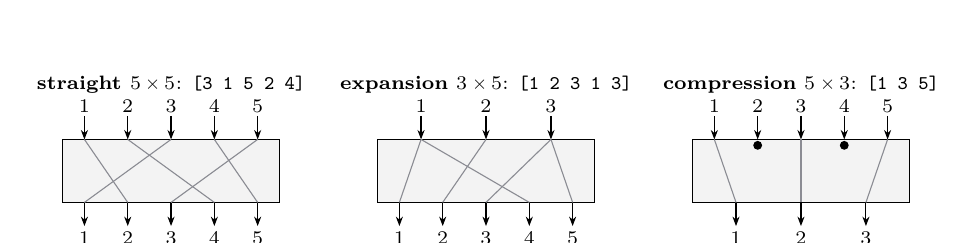
\begin{tikzpicture}[font=\scriptsize,x=5.5mm,y=5mm]
  % straight 5x5: table [3 1 5 2 4]
  \begin{scope}
    \draw[fill=gray!8] (0.5,0) rectangle (5.5,-1.6);
    \node at (3,1.4) {\textbf{straight $5 \times 5$}: \ttx{[3 1 5 2 4]}};
    \foreach \i in {1,...,5} {\draw[-{Stealth[length=1.2mm]}] (\i,0.6) -- (\i,0); \node at (\i,0.85) {\i};
                              \draw[-{Stealth[length=1.2mm]}] (\i,-1.6) -- (\i,-2.2); \node at (\i,-2.5) {\i};}
    \foreach \o/\s in {1/3,2/1,3/5,4/2,5/4} \draw[gray!80!black] (\s,0) -- (\o,-1.6);
  \end{scope}
  % expansion 3x5: table [1 2 3 1 3]
  \begin{scope}[xshift=40mm]
    \draw[fill=gray!8] (0.5,0) rectangle (5.5,-1.6);
    \node at (3,1.4) {\textbf{expansion $3 \times 5$}: \ttx{[1 2 3 1 3]}};
    \foreach \i/\x in {1/1.5,2/3,3/4.5} {\draw[-{Stealth[length=1.2mm]}] (\x,0.6) -- (\x,0); \node at (\x,0.85) {\i};}
    \foreach \i in {1,...,5} {\draw[-{Stealth[length=1.2mm]}] (\i,-1.6) -- (\i,-2.2); \node at (\i,-2.5) {\i};}
    \foreach \o/\x in {1/1.5,2/3,3/4.5,4/1.5,5/4.5} \draw[gray!80!black] (\x,0) -- (\o,-1.6);
  \end{scope}
  % compression 5x3: table [1 3 5]
  \begin{scope}[xshift=80mm]
    \draw[fill=gray!8] (0.5,0) rectangle (5.5,-1.6);
    \node at (3,1.4) {\textbf{compression $5 \times 3$}: \ttx{[1 3 5]}};
    \foreach \i in {1,...,5} {\draw[-{Stealth[length=1.2mm]}] (\i,0.6) -- (\i,0); \node at (\i,0.85) {\i};}
    \foreach \i/\x in {1/1.5,2/3,3/4.5} {\draw[-{Stealth[length=1.2mm]}] (\x,-1.6) -- (\x,-2.2); \node at (\x,-2.5) {\i};}
    \foreach \o/\s in {1.5/1,3/3,4.5/5} \draw[gray!80!black] (\s,0) -- (\o,-1.6);
    \foreach \s in {2,4} \fill (\s,-0.15) circle (1.6pt);
  \end{scope}
\end{tikzpicture}
\end{center}

\textbf{Invertibility.} A straight P-box is invertible: since every input appears exactly once in the table, each output position can be sent back to where it came from. The inverse table is found by writing, for each input position $i$, the output position that holds it. A compression P-box is \emph{not} invertible, because a blocked input bit is simply lost and the inverse would have to invent its value. An expansion P-box is \emph{not} invertible either: an input copied to two outputs would have two candidate sources in the reverse direction, and if the received bits disagree there is no definite answer (more precisely, its reverse is a compression, not an inverse). \imp{Only straight P-boxes are invertible.} This is exactly why AES (all components invertible) uses only straight permutations, while DES (Feistel) can afford an expansion P-box inside its round function.

\begin{worked}[: designing and inverting a straight P-box (slide example)]
\textbf{Q.} Design an $8 \times 8$ permutation table for a straight P-box that moves the two middle bits (bits 4 and 5) of the input to the two ends (bits 1 and 8) of the output, without changing the relative positions of the other bits. Give the inverse table and apply the P-box to \ttx{10011100}.

\textbf{A.} Output bit 1 must take input bit 4 and output bit 8 must take input bit 5. The remaining outputs 2--7 take inputs 1, 2, 3, 6, 7, 8 in their original order. Hence the table is
\[
\text{\ttx{[4 1 2 3 6 7 8 5]}}.
\]
\emph{Inverse:} input 1 went to output 2, input 2 to 3, input 3 to 4, input 4 to 1, input 5 to 8, input 6 to 5, input 7 to 6, input 8 to 7, so the inverse table is \ttx{[2 3 4 1 8 5 6 7]}.\\
\emph{Apply:} input \ttx{10011100} has bits $b_1..b_8 = 1,0,0,1,1,1,0,0$. Output $= b_4 b_1 b_2 b_3 b_6 b_7 b_8 b_5 = \mathbf{11001001}$.\\
\emph{Check:} applying the inverse table to \ttx{11001001} returns \ttx{10011100}; the number of 1s (four) is unchanged, as it must be for any P-box.
\end{worked}

\subsubsection*{S-boxes}
An \textbf{S-box} (substitution box) is a miniature substitution cipher on a few bits: it takes an $n$-bit input and produces an $m$-bit output, where $m$ and $n$ need not be equal. It is normally given as a \textbf{lookup table}: some input bits select the row, the rest select the column, and the cell holds the output. In DES, for instance, a 6-bit input chooses one of 4 rows by its two outer bits and one of 16 columns by its four middle bits, and the cell is a 4-bit value.

\textbf{Linear versus nonlinear.} Write the inputs as $x_1..x_n$ and the outputs as $y_1..y_m$. The S-box is \textbf{linear} if every output is an XOR of inputs, $y_i = a_{i1}x_1 \oplus a_{i2}x_2 \oplus \dots \oplus a_{in}x_n$ with constants $a_{ij} \in \{0,1\}$; then the whole box is a matrix product over GF(2). For example, $y_1 = x_1 \oplus x_2 \oplus x_3$, $y_2 = x_1$ is linear, with matrix $\left(\begin{smallmatrix}1&1&1\\1&0&0\end{smallmatrix}\right)$. If any output contains a product of inputs, such as $y_1 = x_1 x_3 \oplus x_2$, the box is \textbf{nonlinear}. A cipher built only from linear boxes, XORs and P-boxes would be linear as a whole, so every ciphertext bit would be a fixed XOR of plaintext and key bits, and a handful of known plaintext--ciphertext pairs would give a solvable linear system for the key. \imp{The S-boxes are the only nonlinear part of a block cipher, and they must be nonlinear.}

\textbf{Invertibility.} An S-box can be inverted only if it is a one-to-one map, which requires $m = n$ (a $6 \to 4$ box maps 64 inputs onto 16 outputs, so each output has 4 preimages). The slides' $3 \times 3$ example uses the leftmost bit as the row and the two rightmost bits as the column:
\begin{center}\small
\begin{tabular}{@{}c|cccc@{}}
enc & 00 & 01 & 10 & 11\\ \midrule
0 & 011 & 101 & 111 & 100\\
1 & 000 & 010 & 001 & 110\\
\end{tabular}
\qquad
\begin{tabular}{@{}c|cccc@{}}
dec & 00 & 01 & 10 & 11\\ \midrule
0 & 100 & 110 & 101 & 000\\
1 & 011 & 001 & 111 & 010\\
\end{tabular}
\end{center}
Input \ttx{001} (row 0, column 01) encrypts to \ttx{101}, and \ttx{101} (row 1, column 01) in the decryption table gives back \ttx{001}; a script confirms that the two tables undo each other for all 8 inputs.

\subsubsection*{XOR, circular shift, swap, split and combine}
\textbf{Exclusive-or} is addition in GF$(2^n)$, and five properties make it the standard way to mix in a key: \textbf{closure} (the XOR of two $n$-bit words is an $n$-bit word), \textbf{associativity}, \textbf{commutativity}, an \textbf{identity} $00\dots0$, and an \textbf{inverse} for every word, namely the word itself, since $x \oplus x = 00\dots0$. The last property is the important one: whatever is XORed in can be removed by XORing the same value again, $(x \oplus k) \oplus k = x$. A key mixed in this way is called a \textbf{whitener}.

A \textbf{circular shift} rotates an $n$-bit word left or right by $k$ positions. It is invertible, since a left shift by $k$ is undone by a right shift by $k$, and shifting by $k$ is the same as shifting by $k \bmod n$. A \textbf{swap} is the special circular shift by $k = n/2$, exchanging the left and right halves; doing it twice restores the word, so it is \textbf{self-invertible}. A \textbf{split} cuts an $n$-bit word into two $n/2$-bit halves and a \textbf{combine} concatenates two halves; each is the inverse of the other.

\subsection{Product ciphers: confusion, diffusion and rounds \hot}
\likely{One-line theory: ``Define confusion and diffusion; which component provides which?'' or ``What is the avalanche effect?''}
A single small component is easy to analyse and therefore easy to break; a full-size substitution table is secure but impossible to store. Shannon's answer was the \textbf{product cipher}: a cipher that alternates substitutions, permutations and key mixing, so that simple and cheap parts combine into a mapping that behaves like a random one. He named the two properties such a cipher must have.

\textbf{Diffusion} \imp{hides the relationship between the ciphertext and the plaintext}: each ciphertext bit should depend on many or all plaintext bits, so that changing one plaintext bit changes many ciphertext bits. This frustrates an attacker who uses ciphertext statistics (letter or bit frequencies) to guess the plaintext, because any local pattern of the plaintext is spread over the whole block.

\textbf{Confusion} \imp{hides the relationship between the ciphertext and the key}: each ciphertext bit should depend on the key in a complicated way, so that changing one key bit changes most ciphertext bits. This frustrates an attacker who uses known ciphertext to solve for the key.

\textbf{Why S-boxes give confusion.} The key enters the cipher only through XOR, and XOR and P-boxes are linear over GF(2). If the cipher had no S-boxes, every ciphertext bit would be a fixed XOR of plaintext bits and key bits, and a few plaintext--ciphertext pairs would give a linear system whose solution is the key. The nonlinear S-box placed after the key mixing breaks this: its output is a nonlinear function of (data $\oplus$ key), so after a few rounds the ciphertext is a high-degree nonlinear function of the key that cannot be solved for. That is precisely confusion.

\textbf{Why P-boxes give diffusion.} Suppose one input bit of a round changes. It enters one S-box, whose output may change in all its bits (say 2 bits for a $2 \times 2$ box). The P-box then sends those changed bits to \emph{different} S-boxes of the next round, where each again changes up to 2 bits, so the change can grow from 1 bit to 2, 4, 8, \dots\ bits in successive rounds. Without the P-box the changed bits would stay inside the same S-box forever and the change would never spread; the permutation between rounds is what carries it across the block. That is diffusion.

\textbf{Avalanche.} The observable result of good confusion and diffusion is the \textbf{avalanche effect}: flipping one bit of the plaintext or of the key flips about half of the ciphertext bits. Section~\ref{sec:des} shows DES going from 1 differing bit to 29 differing bits out of 64.

\textbf{Rounds.} One layer of S-boxes and P-boxes spreads a bit change only a little, so the layer is repeated. An \textbf{iterated product cipher} applies the same \textbf{round} $N$ times; each round consists of a \textbf{key mixer} (whitener, XOR with a round key), a layer of S-boxes and a P-box. The text between two rounds is called the \textbf{middle text}, and a \textbf{key schedule} (round-key generator) derives the round keys $K_1, \dots, K_N$ from the cipher key, so that each round mixes in a different key. Decryption runs $N$ inverse rounds with the round keys in reverse order.
\begin{center}
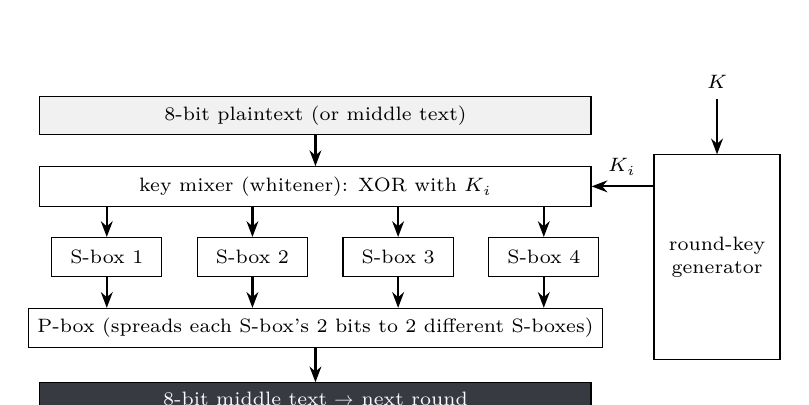
\begin{tikzpicture}[font=\scriptsize,x=1cm,y=1cm]
  \node[draw,fill=gray!10,minimum width=7cm,minimum height=4mm] (pt) at (3.5,0) {8-bit plaintext (or middle text)};
  \node[draw,minimum width=7cm,minimum height=5mm] (km) at (3.5,-0.9) {key mixer (whitener): XOR with $K_i$};
  \foreach \j in {0,...,3} \node[draw,minimum width=1.4cm,minimum height=5mm] (s\j) at (0.85+1.85*\j,-1.8) {S-box \the\numexpr\j+1\relax};
  \node[draw,minimum width=7cm,minimum height=5mm] (pb) at (3.5,-2.7) {P-box (spreads each S-box's 2 bits to 2 different S-boxes)};
  \node[draw,fill=black,text=white,minimum width=7cm,minimum height=4mm] (mt) at (3.5,-3.6) {8-bit middle text $\to$ next round};
  \draw[arr] (pt)--(km); \draw[arr] (pb)--(mt);
  \foreach \j in {0,...,3} {\draw[arr] (km.south -| s\j) -- (s\j); \draw[arr] (s\j) -- (pb.north -| s\j);}
  \node[draw,minimum width=1.6cm,minimum height=2.6cm,align=center] (kg) at (8.6,-1.8) {round-key\\generator};
  \draw[arr] (kg.west |- km) -- node[above]{$K_i$} (km.east);
  \draw[arr] (kg.north) ++(0,0.7) node[above]{$K$} -- (kg.north);
\end{tikzpicture}
\end{center}
\vspace{-2pt}
\centerline{\small One round of the slides' 8-bit product cipher (the slide shows two such rounds).}

\subsection{Feistel ciphers \hot}
\asked{Mid-sem 2024--25 Q6 (5 marks) opens with ``what Feistel structure is prevalent in DES'': the derivation below is that part of the answer.}
Modern block ciphers fall into two classes. \textbf{Feistel ciphers} (DES) use invertible, self-invertible \emph{and noninvertible} components; \textbf{non-Feistel ciphers} (AES) use only invertible components. The problem the Feistel design solves is this: noninvertible components such as an expansion P-box or a $6 \to 4$ S-box mix bits very effectively, but a cipher must be decryptable, and a noninvertible component cannot be run backwards. Feistel's idea is to collect all the noninvertible parts into one function $f$ and never invert it. Its output is only ever \emph{XORed} onto the data, and since XOR is self-inverse, the receiver can cancel it by computing the same $f$ value again and XORing once more.

\textbf{Step 1: the idea in its simplest form.} Let $f$ depend only on the key. Then
\[
\text{encryption: } C = P \oplus f(K), \qquad
\text{decryption: } C \oplus f(K) = P \oplus f(K) \oplus f(K) = P \oplus 00\dots0 = P .
\]
Nothing here requires $f^{-1}$; decryption simply computes $f(K)$ forwards.

\begin{worked}[: the slides' first Feistel example]
\textbf{Q.} Plaintext and ciphertext are 4 bits, the key is 3 bits. $f$ takes the first and third bits of the key, reads them as a decimal number, squares it, and writes the result as 4 bits. Encrypt and decrypt $P = 0111$ with $K = 101$.

\textbf{A.} First and third key bits: $1, 1 \to (11)_2 = 3$; $3^2 = 9 = 1001$, so $f(101) = 1001$.\\
Encryption: $C = P \oplus f(K) = 0111 \oplus 1001 = \mathbf{1110}$.\\
Decryption: $C \oplus f(K) = 1110 \oplus 1001 = 0111 = P$ \checkmark.\\
$f$ is noninvertible (e.g.\ keys $101$ and $111$ both give $1001$, since bit 2 is ignored), yet decryption works because only $f$, never $f^{-1}$, is needed.
\end{worked}

\textbf{Step 2: let the data enter $f$.} A function of the key alone adds nothing per block (it is a fixed XOR, i.e.\ a one-key Vernam). To make $f$ depend on the data while keeping decryption possible, the block is \textbf{split} into a left half $L$ and a right half $R$; $R$ feeds $f$ and $L$ is XORed with the output. This unit is the \textbf{mixer}:
\[
L_2 = L_1 \oplus f(R_1, K), \qquad R_2 = R_1 .
\]
The receiver gets $R_2 = R_1$ unchanged, so it can recompute exactly the same $f(R_1, K)$ and cancel it: $L_2 \oplus f(R_2, K) = L_1 \oplus f(R_1, K) \oplus f(R_1, K) = L_1$. The mixer is therefore \textbf{self-invertible}: applying it twice with the same key is the identity.

\textbf{Step 3: the swapper and more rounds.} The mixer has one flaw: $R$ is never changed, so half of the plaintext appears in clear in the ciphertext. The fix is to add a \textbf{swapper} after the mixer, so that the next round modifies the other half, and to repeat for several rounds. One Feistel round $i$ is then
\[
L_i = R_{i-1}, \qquad R_i = L_{i-1} \oplus f(R_{i-1}, K_i).
\]
\begin{center}
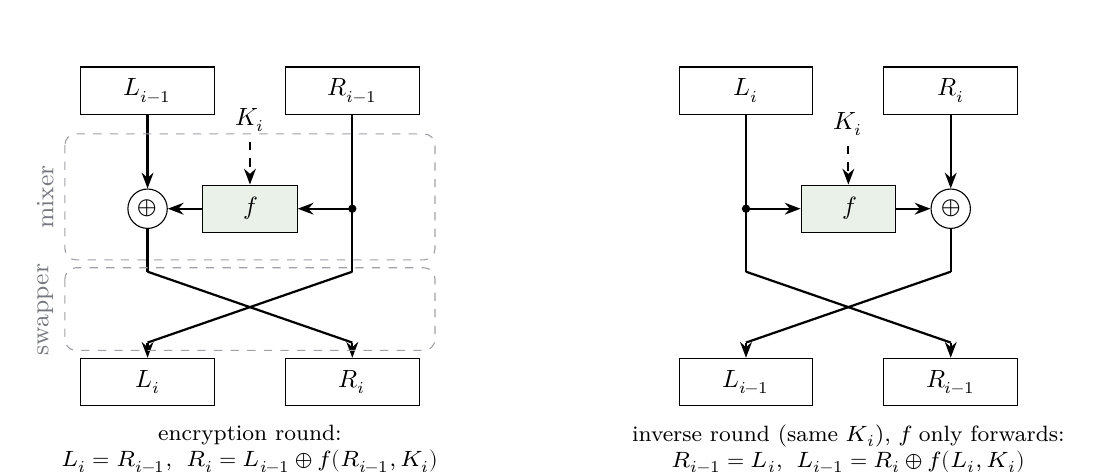
\begin{tikzpicture}[font=\small,x=1cm,y=1cm,hb/.style={draw,minimum width=1.7cm,minimum height=6mm}]
  % ---- left: one Feistel round
  \node[hb] (L0) at (0,0) {$L_{i-1}$};
  \node[hb] (R0) at (2.6,0) {$R_{i-1}$};
  \node[draw,circle,inner sep=0pt,minimum size=5mm] (x) at (0,-1.5) {$\oplus$};
  \node[draw,fill=green!10,minimum width=1.2cm,minimum height=6mm] (f) at (1.3,-1.5) {$f$};
  \draw[arr] (L0) -- (x);
  \draw[thick] (R0) -- (2.6,-2.3);
  \fill (2.6,-1.5) circle (1.5pt);
  \draw[arr] (2.6,-1.5) -- (f);
  \draw[arr] (f) -- (x);
  \draw[arr,dashed] (1.3,-0.65) node[above]{$K_i$} -- (f);
  \draw[thick] (x) -- (0,-2.3);
  \draw[thick] (0,-2.3) -- (2.6,-3.2); \draw[thick] (2.6,-2.3) -- (0,-3.2);
  \node[hb] (L1) at (0,-3.7) {$L_i$};
  \node[hb] (R1) at (2.6,-3.7) {$R_i$};
  \draw[arr] (0,-3.2) -- (L1); \draw[arr] (2.6,-3.2) -- (R1);
  \draw[gray,dashed,rounded corners] (-1.05,-0.55) rectangle (3.65,-2.15);
  \draw[gray,dashed,rounded corners] (-1.05,-2.25) rectangle (3.65,-3.3);
  \node[gray!60!black,rotate=90] at (-1.3,-1.35) {mixer};
  \node[gray!60!black,rotate=90] at (-1.3,-2.78) {swapper};
  \node[align=center,font=\footnotesize] at (1.3,-4.55) {encryption round:\\$L_i = R_{i-1}$,\; $R_i = L_{i-1} \oplus f(R_{i-1}, K_i)$};
  % ---- right: inverse of the round, derived
  \begin{scope}[xshift=7.6cm]
    \node[hb] (a) at (0,0) {$L_i$};
    \node[hb] (b) at (2.6,0) {$R_i$};
    \node[draw,circle,inner sep=0pt,minimum size=5mm] (y) at (2.6,-1.5) {$\oplus$};
    \node[draw,fill=green!10,minimum width=1.2cm,minimum height=6mm] (g) at (1.3,-1.5) {$f$};
    \draw[thick] (a) -- (0,-2.3);
    \fill (0,-1.5) circle (1.5pt);
    \draw[arr] (0,-1.5) -- (g);
    \draw[arr] (g) -- (y);
    \draw[arr] (b) -- (y);
    \draw[arr,dashed] (1.3,-0.7) node[above]{$K_i$} -- (g);
    \draw[thick] (y) -- (2.6,-2.3);
    \draw[thick] (2.6,-2.3) -- (0,-3.2);
    \draw[thick] (0,-2.3) -- (2.6,-3.2);
    \node[hb] (c) at (0,-3.7) {$L_{i-1}$};
    \node[hb] (d) at (2.6,-3.7) {$R_{i-1}$};
    \draw[arr] (0,-3.2) -- (c); \draw[arr] (2.6,-3.2) -- (d);
    \node[align=center,font=\footnotesize] at (1.3,-4.55) {inverse round (same $K_i$), $f$ only forwards:\\$R_{i-1} = L_i$,\; $L_{i-1} = R_i \oplus f(L_i, K_i)$};
  \end{scope}
\end{tikzpicture}
\end{center}

\begin{mustknow}[: why a Feistel round is invertible even if $f$ is not]
Given the round output $(L_i, R_i)$, the first equation hands back $R_{i-1} = L_i$ directly. Knowing $R_{i-1}$, the receiver can \emph{recompute} $f(R_{i-1}, K_i)$ forwards and XOR it away:
\[
R_i \oplus f(L_i, K_i) = L_{i-1} \oplus f(R_{i-1}, K_i) \oplus f(R_{i-1}, K_i) = L_{i-1}.
\]
$f$ is only ever evaluated, never inverted, so it may be many-to-one (expansion P-box, $6 \to 4$ S-boxes). Since the mixer and the swapper are each self-inverse, decryption is the same structure run with the round keys in reverse order ($K_N, \dots, K_1$).
\end{mustknow}

In the slides' two-round final design (slide L7-29), both rounds end with a swapper, so the decryption circuit applies the swapper first and then the mixer, round keys $K_2$ then $K_1$. DES removes the swapper from the \emph{last} round; then encryption and decryption are literally the same algorithm and only the key order changes. The toy below uses that DES convention.

\begin{worked}[: two-round Feistel cipher with a noninvertible $f$]
\textbf{Q.} An 8-bit Feistel cipher has 4-bit halves and two rounds; round 1 has a swapper, round 2 does not (DES convention). The round function is $f(R, K) = (R \oplus K)^2 \bmod 16$. Encrypt $L_0 R_0 = 1010\;0111$ with $K_1 = 0100$, $K_2 = 1001$, then decrypt with the same algorithm and the keys reversed. Show that $f$ is not invertible.

\textbf{A.} $f$ is not invertible: $0011^2 = 9$ and $0101^2 = 25 \equiv 9 \pmod{16}$, so two inputs give $1001$; in fact $x^2 \bmod 16$ only takes the values 0, 1, 4, 9.
\begin{center}\small
\begin{tabular}{@{}lccccc@{}}
\toprule
Round & input $L$, $R$ & $R \oplus K$ & $f$ & $L \oplus f$ & output (after swap?)\\
\midrule
Enc 1 ($K_1 = 0100$) & 1010, 0111 & 0011 & 1001 & 0011 & swap $\to$ 0111, 0011\\
Enc 2 ($K_2 = 1001$) & 0111, 0011 & 1010 & 0100 & 0011 & no swap $\to$ \textbf{0011, 0011}\\
\midrule
Dec 1 ($K_2 = 1001$) & 0011, 0011 & 1010 & 0100 & 0111 & swap $\to$ 0011, 0111\\
Dec 2 ($K_1 = 0100$) & 0011, 0111 & 0011 & 1001 & 1010 & no swap $\to$ \textbf{1010, 0111}\\
\bottomrule
\end{tabular}
\end{center}
Ciphertext $= \mathbf{0011\,0011}$; decryption returns $1010\,0111 = P$ \checkmark. Each decryption round recomputes exactly the $f$ value of the matching encryption round (1001 and 0100), because the half fed to $f$ is passed through unchanged.
\end{worked}

\subsection{Non-Feistel ciphers}
A \textbf{non-Feistel cipher} uses only invertible components, and every component of the encryption has a matching inverse component in the decryption. This constrains the parts: S-boxes must have as many output bits as input bits, and expansion and compression P-boxes are not allowed, because they cannot be inverted. Since there is no $f$ whose output is XORed in, there is also no need to split the block into halves; each round transforms the whole block. The slides' 8-bit product cipher above is a non-Feistel cipher: XOR (self-invertible), $2 \times 2$ invertible S-boxes and a straight P-box, so each round is invertible and decryption runs the inverse rounds with keys $K_2$, $K_1$. AES is the real example.

\begin{center}\small
\begin{tabularx}{\textwidth}{@{}l X X@{}}
\toprule
 & \textbf{Feistel} (DES) & \textbf{Non-Feistel} (AES)\\
\midrule
Components & invertible, self-invertible and noninvertible & only invertible ($n \times n$ S-boxes, straight P-boxes)\\
Block handling & split into $L$, $R$; mixer $L \oplus f(R, K)$, then swapper & whole block in every round\\
Decryption & same structure, round keys reversed; $f$ never inverted & inverse components in reverse order, round keys reversed\\
\bottomrule
\end{tabularx}
\end{center}

\subsection{Attacks on modern block ciphers}
\textbf{Brute force} on the key is normally infeasible because keys are long (but $2^{56}$ for DES is not). The serious attacks exploit the structure of the rounds.
\begin{itemize}
  \item \textbf{Differential cryptanalysis} (Biham and Shamir) is a \textbf{chosen-plaintext} attack. Eve submits pairs of plaintexts with a chosen difference $P_1 \oplus P_2$ and studies the output difference $C_1 \oplus C_2$; a weak cipher propagates certain differences with high probability, which reveals key bits. The slides' extreme case is a cipher that is only an XOR with the key: $C_1 \oplus C_2 = (P_1 \oplus K) \oplus (P_2 \oplus K) = P_1 \oplus P_2$, so the difference passes through untouched and is independent of the key. Nonlinear S-boxes are what destroy this predictability.
  \item \textbf{Linear cryptanalysis} (Matsui) is a \textbf{known-plaintext} attack. If an S-box is not fully nonlinear, some XOR of input and output bits equals an XOR of key bits with probability noticeably different from $1/2$; collecting many plaintext--ciphertext pairs and counting how often such an equation holds reveals those key bits.
\end{itemize}

\subsection{Modern stream ciphers}
A \textbf{modern stream cipher} encrypts and decrypts $r$ bits at a time: the plaintext $P = p_n \dots p_2 p_1$, ciphertext $C = c_n \dots c_2 c_1$ and key stream $K = k_n \dots k_2 k_1$ consist of $r$-bit words, and $c_i = p_i \oplus k_i$, $p_i = c_i \oplus k_i$. Encryption and decryption are a single XOR, so the cipher is fast and needs no padding; all of its security lies in the \textbf{key stream}, which must look random and must never be reused. Stream ciphers are classified by how the key stream is produced.

\textbf{Synchronous stream ciphers.} In a \textbf{synchronous} stream cipher the key stream is \emph{independent} of the plaintext and the ciphertext; it is generated from the key alone, and sender and receiver must stay in step (synchronised) with each other. The ideal case is the \textbf{one-time pad}: a truly random key stream as long as the message, used once, giving perfect secrecy, at the price that a key as long as all the traffic must be shared in advance. Practical synchronous ciphers replace the random pad by a pseudorandom generator such as a \textbf{feedback shift register} (FSR). An FSR has $m$ one-bit cells $b_{m-1} \dots b_1 b_0$; at each step $b_0$ is output as a key bit, all cells shift right, and the new leftmost bit is computed by a \textbf{feedback function} of the old cells. In a \textbf{linear} FSR (LFSR) the feedback is an XOR of selected cells, so it costs one gate. With a well-chosen feedback an $m$-cell LFSR runs through all $2^m - 1$ nonzero states before repeating, the maximum period. Because it is linear, however, about $2m$ consecutive key-stream bits are enough to solve for the feedback taps and predict the rest, so real designs use a \textbf{nonlinear} FSR or combine several LFSRs nonlinearly.

\begin{worked}[: LFSR key stream (Forouzan style)]
\textbf{Q.} Create a 4-cell LFSR with feedback $b_4 = b_1 \oplus b_0$ (the new $b_3$). Show the output for 20 shifts if the seed $b_3 b_2 b_1 b_0$ is $0001$, and find the period.

\textbf{A.} Each step outputs $b_0$, then the state becomes $(b_1 \oplus b_0)\, b_3\, b_2\, b_1$.
\begin{center}\scriptsize\setlength{\tabcolsep}{2.2pt}
\begin{tabular}{@{}l*{16}{c}@{}}
\toprule
step & 0&1&2&3&4&5&6&7&8&9&10&11&12&13&14&15\\
\midrule
state & 0001&1000&0100&0010&1001&1100&0110&1011&0101&1010&1101&1110&1111&0111&0011&\textbf{0001}\\
out $b_0$ & 1&0&0&0&1&0&0&1&1&0&1&0&1&1&1&1\\
\bottomrule
\end{tabular}
\end{center}
At step 15 the state is the seed again, so the key stream repeats with period $\mathbf{15} = 2^4 - 1$ (maximum: every nonzero state appears once). The 20 output bits are $\mathbf{1000\,1001\,1010\,1111\,0001}$.\\
\emph{Check:} the bits 16--20 ($1\,0001$) repeat bits 1--5 ($1\,0001$), as the period predicts.
\end{worked}

\textbf{Nonsynchronous (self-synchronising) stream ciphers.} In a \textbf{nonsynchronous} stream cipher each key-stream element depends on previous plaintext or ciphertext elements. The usual form is \textbf{self-synchronising}: the key stream is computed from the key and the last few ciphertext bits (as in CFB mode). If a ciphertext bit is corrupted or lost, the receiver's key stream is wrong only while the bad bit is inside its window, and decryption recovers by itself once the window has passed.

\textbf{Error behaviour.} In a synchronous cipher a flipped ciphertext bit spoils only the matching plaintext bit, but a lost or inserted bit shifts the two key streams against each other and garbles everything after it until the parties resynchronise. In a self-synchronising cipher a single error spoils a few following bits as well, but a lost bit is recovered from automatically.

\begin{fixbox}
\begin{itemize}
  \item Feistel example (L7 slide 25): the problem says $f$ uses the \emph{first and third} key bits, but the solution ``extracts the first and second bits to get 11''. For $K = 101$ the first and second bits are \ttx{10} $= 2$, giving $f = 0100$; only the first and third bits give \ttx{11} $= 3$ and the stated $f = 1001$, $C = 1110$. Use first and third.
  \item Stream ciphers (L7 slide 39): the line reads ``In a synchronous stream cipher the key is independent of the plaintext or ciphertext''; it is easily read as ``asynchronous'' (the old version of these notes did so). The key-independent class is \textbf{synchronous}. Some books (Stallings) call the \emph{other} class, the self-synchronising ciphers, ``asynchronous'', so do not mix the words up.
  \item Nonlinear S-box (L7 slide 18): over GF(2), $x^3 = x$ and $x^2 = x$, so the slide's $y_1 = x_1^3 + x_2 = x_1 + x_2$ is actually linear; the box is nonlinear because of the product term $x_1 x_2$ in $y_2 = x_1^2 + x_1x_2 + x_3$.
\end{itemize}
\end{fixbox}

% College Lecture 8: DES (Forouzan ch. 6). Every number recomputed by scratchpad/des/verify.py, which implements
% full DES (checked against the Stallings test vector 0123456789ABCDEF/133457799BBCDFF1 -> 85E813540F0AB405).
\section{Data Encryption Standard (DES)}\label{sec:des}

The \textbf{Data Encryption Standard} is the symmetric-key block cipher published by NIST (then NBS) in 1977, based on IBM's Lucifer. It encrypts a \textbf{64-bit block} with a \textbf{56-bit key} through \textbf{16 Feistel rounds}. The key is normally supplied as 64 bits, of which 8 are parity bits that are dropped, and a key schedule derives sixteen \textbf{48-bit round keys} $K_1, \dots, K_{16}$ from it. Decryption is done by the \textbf{reverse cipher}, which is the same algorithm with the round keys used in the order $K_{16}, \dots, K_1$. DES has since been replaced by AES because its key is too short, but its structure is the standard example of a Feistel cipher (Section~\ref{sec:modern}).

\subsection{DES structure \hot}
\asked{2024--25 Q6 (5 marks): Feistel structure, block diagrams of the DES algorithm and the round function, pseudocode for the S-box substitution and key generation.}
Encryption consists of an \textbf{initial permutation} (IP) of the 64-bit plaintext, sixteen rounds, and a \textbf{final permutation} (FP). After IP the block is split into a left half $L_0$ and a right half $R_0$ of 32 bits each. Each round $i$ takes $(L_{i-1}, R_{i-1})$ and produces $(L_i, R_i)$ with a Feistel \textbf{mixer} followed by a \textbf{swapper}:
\[
L_i = R_{i-1}, \qquad R_i = L_{i-1} \oplus f(R_{i-1}, K_i),
\]
where $f$ is the DES function described below. Round 16 has no swapper, and after it the halves are combined and passed through FP to give the 64-bit ciphertext. The block diagrams of the whole algorithm, of one round and of the key generator are drawn in the exam answer at the end of the key-generation subsection.

\subsection{Initial and final permutations}
IP and FP are keyless \textbf{straight P-boxes} ($64 \times 64$) that are inverses of each other: FP $=$ IP$^{-1}$. The IP table is read row by row; entry $j$ is the input bit that goes to output position $j$.
\begin{center}\scriptsize\setlength{\tabcolsep}{3.2pt}
\begin{tabular}{@{}*{8}{c}@{}}
\multicolumn{8}{c}{\textbf{Initial permutation}}\\ \midrule
58&50&42&34&26&18&10&02\\ 60&52&44&36&28&20&12&04\\ 62&54&46&38&30&22&14&06\\ 64&56&48&40&32&24&16&08\\
57&49&41&33&25&17&09&01\\ 59&51&43&35&27&19&11&03\\ 61&53&45&37&29&21&13&05\\ 63&55&47&39&31&23&15&07\\
\end{tabular}
\qquad
\begin{tabular}{@{}*{8}{c}@{}}
\multicolumn{8}{c}{\textbf{Final permutation}}\\ \midrule
40&08&48&16&56&24&64&32\\ 39&07&47&15&55&23&63&31\\ 38&06&46&14&54&22&62&30\\ 37&05&45&13&53&21&61&29\\
36&04&44&12&52&20&60&28\\ 35&03&43&11&51&19&59&27\\ 34&02&42&10&50&18&58&26\\ 33&01&41&09&49&17&57&25\\
\end{tabular}
\end{center}
So output bit 1 of IP is input bit 58, and input bit 1 lands in output position 40; correspondingly the FP table has 40 in position 1 (FP puts it back).

\textbf{Why they add no security.} Both permutations are fixed, keyless and published. An attacker who knows a plaintext can apply IP to it himself, and can apply IP $=$ FP$^{-1}$ to the ciphertext, which strips both permutations off and leaves exactly the 16 rounds to attack. \imp{IP and FP have no cryptographic significance}; they are usually explained as a convenience for loading 8-bit bytes into 1970s hardware.

\begin{worked}[: initial permutation (Forouzan style)]
\textbf{Q.} Find the output of the initial permutation for the input \ttx{0x0002 0000 0000 0001} and show that FP restores it.

\textbf{A.} The input has only two 1-bits: hex digit 4 is \ttx{2} $= 0010$, i.e.\ bit $12 + 3 = \mathbf{15}$, and the last bit, \textbf{64}. In the IP table, 15 is entry 63 and 64 is entry 25, so the output has 1s exactly in positions 25 and 63:
\[
\text{IP}(\ttx{0002000000000001}) = \ttx{0x0000 0080 0000 0002}.
\]
(Bit 25 is the leading bit of hex digit 7, giving \ttx{8}; bit 63 is the third bit of hex digit 16, giving \ttx{2}.)\\
\emph{Check:} in the FP table, entry 15 is 63 and entry 64 is 25, so FP moves bits 63 and 25 back to positions 15 and 64.
\end{worked}

\subsection{Rounds: mixer, swapper and the reverse cipher}
Each round is a Feistel round (Section~\ref{sec:modern}): the \textbf{mixer} replaces $L_{i-1}$ by $L_{i-1} \oplus f(R_{i-1}, K_i)$ and leaves $R_{i-1}$ alone, and the \textbf{swapper} exchanges the halves. The mixer is invertible because of the XOR: given the output, the receiver still has $R_{i-1}$, recomputes $f(R_{i-1}, K_i)$ and XORs it away. The mixer and the swapper are each \textbf{self-inverse}: applying either twice (the mixer with the same key) gives back the input.

\textbf{Why decryption is the same algorithm with keys reversed.} Write encryption as the sequence of operations
\[
\text{IP},\ M_{K_1},\ S,\ M_{K_2},\ S,\ \dots,\ M_{K_{15}},\ S,\ M_{K_{16}},\ \text{FP},
\]
where $M_K$ is the mixer with key $K$ and $S$ the swapper. The inverse of a sequence applies the inverses of its steps in reverse order, and here FP$^{-1} =$ IP, $M_K^{-1} = M_K$, $S^{-1} = S$ and IP$^{-1} =$ FP. Decryption is therefore
\[
\text{IP},\ M_{K_{16}},\ S,\ M_{K_{15}},\ S,\ \dots,\ S,\ M_{K_1},\ \text{FP}.
\]
This is exactly the encryption algorithm with the round keys in the order $K_{16}, \dots, K_1$. The match works only because round 16 has no swapper: with a swapper there, the inverse would start with $S$ and would no longer have the same shape as the cipher. \imp{The last round has no swapper so that the reverse cipher is the cipher itself with reversed round keys.} (Equivalently, Stallings lets all 16 rounds swap and adds a 32-bit swap before FP; the two descriptions give the same ciphertext.)

The slides' pseudocode for the cipher (Forouzan):
\begin{center}
\begin{minipage}{0.8\textwidth}\small
\textbf{Cipher} (plainBlock[64], RoundKeys[16, 48], cipherBlock[64])\\
\{\\
\hspace*{1.5em}\textbf{permute} (64, 64, plainBlock, inBlock, \emph{InitialPermutationTable})\\
\hspace*{1.5em}\textbf{split} (64, 32, inBlock, leftBlock, rightBlock)\\
\hspace*{1.5em}\textbf{for} (round $= 1$ to 16)\\
\hspace*{1.5em}\{\\
\hspace*{3em}\textbf{mixer} (leftBlock, rightBlock, RoundKeys[round])\\
\hspace*{3em}\textbf{if} (round $\neq 16$) \textbf{swapper} (leftBlock, rightBlock)\\
\hspace*{1.5em}\}\\
\hspace*{1.5em}\textbf{combine} (32, 64, leftBlock, rightBlock, outBlock)\\
\hspace*{1.5em}\textbf{permute} (64, 64, outBlock, cipherBlock, \emph{FinalPermutationTable})\\
\}
\end{minipage}
\end{center}
Here mixer does $T \leftarrow f(\text{rightBlock}, K)$, leftBlock $\leftarrow$ leftBlock $\oplus\ T$, and swapper exchanges the two blocks through a temporary copy.

\subsection{The DES function $f(R_{i-1}, K_i)$ \hot}
The DES function is the heart of the cipher and the only place where the key enters. It applies the 48-bit round key to the 32-bit right half and returns 32 bits, through four steps.

\textbf{1. Expansion P-box (32 $\to$ 48).} $R_{i-1}$ has 32 bits but $K_i$ has 48, and the S-boxes need 6-bit inputs, so $R_{i-1}$ is expanded first. It is viewed as eight 4-bit sections; each section is widened to 6 bits by adding, on its left, the last bit of the previous section and, on its right, the first bit of the next section (cyclically, so section 1 borrows bit 32 and section 8 borrows bit 1):
\begin{center}\scriptsize\setlength{\tabcolsep}{3.2pt}
\begin{tabular}{@{}*{6}{c}@{\hspace{14pt}}*{6}{c}@{}}
32&01&02&03&04&05 & 04&05&06&07&08&09\\
08&09&10&11&12&13 & 12&13&14&15&16&17\\
16&17&18&19&20&21 & 20&21&22&23&24&25\\
24&25&26&27&28&29 & 28&29&30&31&32&01\\
\end{tabular}
\end{center}
The 16 bits that appear twice are the first and fourth bits of every section (1, 4, 5, 8, \dots, 29, 32). This duplication is deliberate: a bit at the edge of a section reaches two neighbouring S-boxes, so changing it changes the input of two S-boxes, which is what makes the avalanche grow quickly. Being an expansion P-box, this step is not invertible, which a Feistel cipher can afford.

\textbf{2. Whitener.} The 48-bit expanded half is XORed with the 48-bit round key $K_i$. This is the only point at which the key influences the round.

\textbf{3. S-boxes (48 $\to$ 32).} The 48 bits are cut into eight 6-bit groups, and group $j$ enters S-box $S_j$, which outputs 4 bits. \imp{The S-boxes do the real mixing (confusion)}, being the only nonlinear part of DES. Each S-box is a table of 4 rows and 16 columns. For a 6-bit input $b_1 b_2 b_3 b_4 b_5 b_6$:
\[
\text{row} = (b_1 b_6)_2 \in \{0..3\}, \qquad \text{column} = (b_2 b_3 b_4 b_5)_2 \in \{0..15\},
\]
and the cell is the 4-bit output. The outer bits pick one of four substitutions and the middle bits are substituted by it; every row of every S-box is a permutation of $0..15$ (checked by script), so each output value has exactly 4 preimages and the box as a whole is not invertible. The eight S-boxes are different. S-box 1:
\begin{center}\small\setlength{\tabcolsep}{3.5pt}
\begin{tabular}{@{}c|*{16}{c}@{}}
S1 & 0&1&2&3&4&5&6&7&8&9&10&11&12&13&14&15\\ \midrule
0 & 14&4&13&1&2&15&11&8&3&10&6&12&5&9&0&7\\
1 & 0&15&7&4&14&2&13&1&10&6&12&11&9&5&3&8\\
2 & 4&1&14&8&13&6&2&11&15&12&9&7&3&10&5&0\\
3 & 15&12&8&2&4&9&1&7&5&11&3&14&10&0&6&13\\
\end{tabular}
\end{center}

\textbf{4. Straight P-box (32 $\to$ 32).} The 32 S-box output bits are permuted by a straight P-box; entry $j$ is the input bit sent to output $j$, so the seventh input bit becomes the second output bit:
\begin{center}\scriptsize\setlength{\tabcolsep}{3.2pt}
\begin{tabular}{@{}*{8}{c}@{}}
16&07&20&21&29&12&28&17\\ 01&15&23&26&05&18&31&10\\ 02&08&24&14&32&27&03&09\\ 19&13&30&06&22&11&04&25\\
\end{tabular}
\end{center}
Its job is diffusion: the 4 output bits of each S-box are sent to positions that feed different S-boxes in the next round.

\begin{worked}[: S-box lookup]
\likely{``The input to S-box 1 is \ttx{100011}. What is the output?'' (Forouzan's standard S-box question.)}
\textbf{Q.} (a) The input to S-box 1 is \ttx{100011}. What is the output? (b) The input to S-box 8 is \ttx{000000}. What is the output?

\textbf{A.} (a) Outer bits $b_1 b_6 = 1\,1$, so row $= (11)_2 = 3$. Middle bits $b_2..b_5 = 0001$, so column $= 1$. In S1, row 3, column 1 holds $12$, so the output is $\mathbf{1100}$.\\
(b) Outer bits $0\,0 \Rightarrow$ row 0; middle bits $0000 \Rightarrow$ column 0. S8 row 0 begins \ttx{13 2 8 4 \dots}, so the output is $13 = \mathbf{1101}$.\\
\emph{More S1 lookups for practice:} \ttx{000000} $\to$ row 0, col 0 $\to 14 = 1110$; \ttx{111111} $\to$ row 3, col 15 $\to 13 = 1101$; \ttx{011011} $\to$ row 1, col 13 $\to 5 = 0101$.
\end{worked}

\begin{trap}[: row and column bits]
The row is the \emph{first and last} bit (not the first two), and the column is the \emph{middle four}. Numbering starts at 0 for both rows and columns. Writing the answer as a decimal (12) without converting it to 4 bits (\ttx{1100}) loses the mark that the output is a 4-bit word.
\end{trap}

\begin{worked}[: one full DES round (Forouzan's trace: $P = $ \ttx{123456ABCD132536}, key \ttx{AABB09182736CCDD})]
\textbf{Q.} After the initial permutation, $L_0 = $ \ttx{14A7D678} and $R_0 = $ \ttx{18CA18AD}; the first round key is $K_1 = $ \ttx{194CD072DE8C}. Compute $f(R_0, K_1)$, $L_1$ and $R_1$.

\textbf{A.} $R_0 = 0001\,1000\,1100\,1010\,0001\,1000\,1010\,1101$. Expansion (each 4-bit section borrows its neighbours' edge bits) gives $E(R_0) = $ \ttx{8F16540F155A}; XOR with $K_1$ gives \ttx{965A847DCBD6}. The eight 6-bit groups go through the S-boxes:
\begin{center}\small\setlength{\tabcolsep}{4pt}
\begin{tabular}{@{}lcccccccc@{}}
\toprule
S-box & 1 & 2 & 3 & 4 & 5 & 6 & 7 & 8\\
\midrule
$E(R_0)$ group & 100011 & 110001 & 011001 & 010100 & 000011 & 110001 & 010101 & 011010\\
$K_1$ group & 000110 & 010100 & 110011 & 010000 & 011100 & 101101 & 111010 & 001100\\
XOR (input) & 100101 & 100101 & 101010 & 000100 & 011111 & 011100 & 101111 & 010110\\
row, col & 3, 2 & 3, 2 & 2, 5 & 0, 2 & 1, 15 & 0, 14 & 3, 7 & 0, 11\\
output & 8 & 10 & 15 & 14 & 6 & 5 & 7 & 14\\
\bottomrule
\end{tabular}
\end{center}
S-box output $= $ \ttx{8AFE657E}; the straight P-box gives $f(R_0, K_1) = $ \ttx{4EDF35EC}. Then
\[
L_1 = R_0 = \ttx{18CA18AD}, \qquad R_1 = L_0 \oplus f = \ttx{14A7D678} \oplus \ttx{4EDF35EC} = \ttx{5A78E394}.
\]
\emph{Check:} this is the round-1 output in Forouzan's table; continuing all 16 rounds (round 16 output \ttx{19BA9212 CF26B472}, no swap) and FP gives the ciphertext \ttx{C0B7A8D05F3A829C}, and running the same program with the keys reversed returns the plaintext.
\end{worked}

\subsection{Key generation \hot}
The round-key generator must turn one 56-bit cipher key into sixteen different 48-bit round keys, cheaply and so that every key bit influences many rounds. It works in four steps.
\begin{enumerate}
  \item \textbf{Parity drop (64 $\to$ 56).} The key is supplied as 64 bits in which bits 8, 16, 24, \dots, 64 are parity bits (each key byte has odd parity). A compression permutation (PC-1) discards these 8 bits and permutes the remaining 56.
  \item \textbf{Split.} The 56 bits are split into two 28-bit halves $C_0$ and $D_0$.
  \item \textbf{Shift.} In round $i$ both halves are circularly shifted left, by \textbf{1 bit in rounds 1, 2, 9 and 16} and by 2 bits in all other rounds, giving $C_i$ and $D_i$.
  \item \textbf{Compression P-box (56 $\to$ 48).} $C_i \| D_i$ passes through a compression P-box (PC-2) that blocks 8 of the 56 bits and permutes the other 48; the result is $K_i$.
\end{enumerate}
\textbf{Why it is built this way.} Because the halves are rotated before each compression, a different selection and arrangement of key bits reaches the S-boxes in every round; each key bit ends up in 12 to 15 of the 16 round keys (about 14 on average, counted by script). The shift amounts add up to $4 \times 1 + 12 \times 2 = 28$, a full rotation of a 28-bit half, so $C_{16} = C_0$ and $D_{16} = D_0$. This lets the decryption side generate $K_{16}, \dots, K_1$ on the fly by \emph{right} shifts starting from the original halves.

\begin{worked}[: first round key (same key as the trace above)]
\textbf{Q.} For the key \ttx{AABB09182736CCDD}, find $C_0$, $D_0$, $C_1$, $D_1$ and $K_1$.

\textbf{A.} Parity drop gives the 56-bit key \ttx{C3C033A33F0CFA}, so $C_0 = $ \ttx{C3C033A}, $D_0 = $ \ttx{33F0CFA}. Round 1 shifts by 1 bit:
\begin{center}\small
\begin{tabular}{@{}lll@{}}
$C_0 = 1100\,0011\,1100\,0000\,0011\,0011\,1010$ & $\xrightarrow{\text{rotl } 1}$ & $C_1 = 1000\,0111\,1000\,0000\,0110\,0111\,0101 = $ \ttx{8780675}\\
$D_0 = 0011\,0011\,1111\,0000\,1100\,1111\,1010$ & $\xrightarrow{\text{rotl } 1}$ & $D_1 = 0110\,0111\,1110\,0001\,1001\,1111\,0100 = $ \ttx{67E19F4}\\
\end{tabular}
\end{center}
The compression P-box applied to $C_1 \| D_1$ gives $K_1 = $ \ttx{194CD072DE8C}, the key used in the round trace above.\\
\emph{Check:} in each half the leading bit moved to the end (e.g.\ $C_0$ starts with 1 and $C_1$ ends with 1).
\end{worked}

\begin{worked}[: 2024--25 Q6 (5 marks), answer as it should be written]
\textbf{Q.} In DES, what Feistel structure is prevalent? Use flow diagrams and key generation to define, with block diagrams, (1) the algorithm for DES and (2) the algorithm for the round function. How would you write the pseudocode for the substitution block and key generation?

\textbf{A. Feistel structure.} DES is a Feistel cipher: the 64-bit block (after IP) is split into 32-bit halves, and each of the 16 rounds applies a mixer and a swapper,
\[
L_i = R_{i-1}, \qquad R_i = L_{i-1} \oplus f(R_{i-1}, K_i), \qquad i = 1..16 \text{ (no swap in round 16).}
\]
All noninvertible parts (expansion P-box, $6 \to 4$ S-boxes) are inside $f$, whose output is only XORed in. Since $R_{i-1} = L_i$ is available to the receiver, $L_{i-1} = R_i \oplus f(L_i, K_i)$; so $f$ never has to be inverted, and decryption is the same algorithm with keys $K_{16}, \dots, K_1$.

\textbf{(1) DES algorithm and key generation.}
\begin{center}
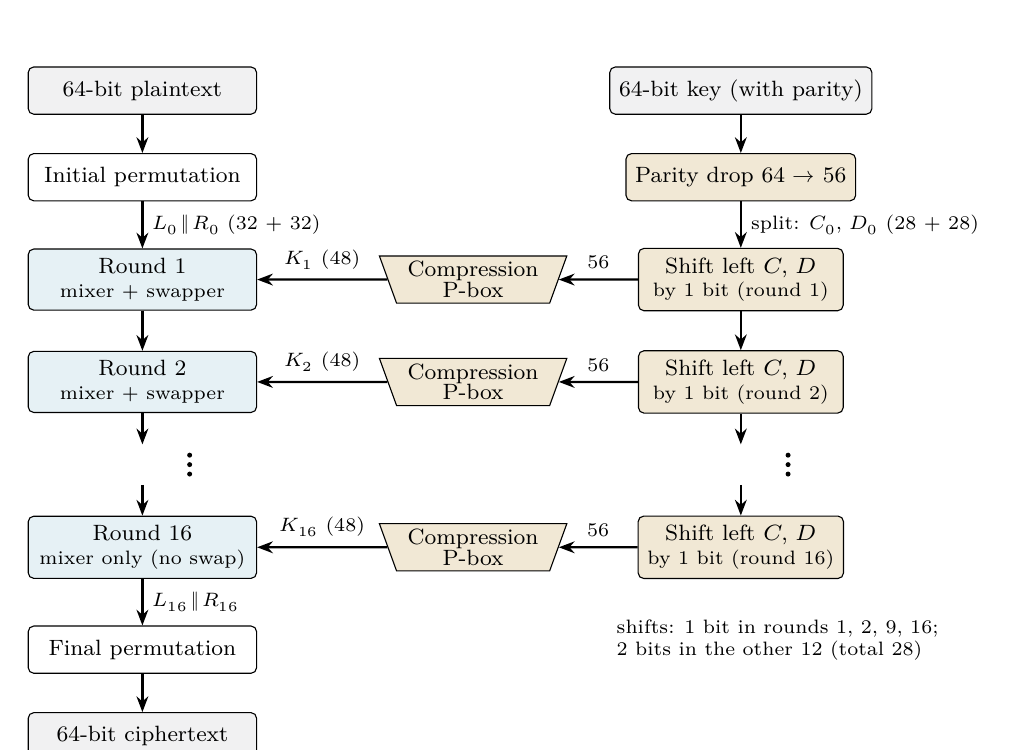
\begin{tikzpicture}[font=\footnotesize,x=1cm,y=1cm,
  db/.style={draw,rounded corners=2pt,minimum width=2.9cm,minimum height=6mm,align=center},
  kb/.style={draw,rounded corners=2pt,fill=yellow!15,minimum width=2.6cm,minimum height=6mm,align=center},
  cb/.style={draw,fill=yellow!15,trapezium,trapezium angle=70,shape border rotate=180,minimum width=2.2cm,minimum height=6mm,align=center,inner sep=1pt}]
  % data path
  \node[db,fill=gray!10] (pt) at (0,0) {64-bit plaintext};
  \node[db] (ip) at (0,-1.1) {Initial permutation};
  \node[db,fill=cyan!8] (r1) at (0,-2.4) {Round 1\\[-1pt]\scriptsize mixer + swapper};
  \node[db,fill=cyan!8] (r2) at (0,-3.7) {Round 2\\[-1pt]\scriptsize mixer + swapper};
  \node[inner sep=0pt,minimum size=5mm] (dd) at (0,-4.75) {}; \foreach \d in {-0.12,0,0.12} \fill (0.6,-4.75+\d) circle (0.9pt);
  \node[db,fill=cyan!8] (r16) at (0,-5.8) {Round 16\\[-1pt]\scriptsize mixer only (no swap)};
  \node[db] (fp) at (0,-7.1) {Final permutation};
  \node[db,fill=gray!10] (ct) at (0,-8.2) {64-bit ciphertext};
  \draw[arr] (pt)--(ip);
  \draw[arr] (ip)-- node[right,font=\scriptsize]{$L_0 \,\|\, R_0$ (32 + 32)} (r1);
  \draw[arr] (r1)--(r2); \draw[arr] (r2)--(dd); \draw[arr] (dd)--(r16);
  \draw[arr] (r16)-- node[right,font=\scriptsize]{$L_{16} \,\|\, R_{16}$} (fp); \draw[arr] (fp)--(ct);
  % key generator
  \node[kb,fill=gray!10] (k64) at (7.6,0) {64-bit key (with parity)};
  \node[kb] (pd) at (7.6,-1.1) {Parity drop 64 $\to$ 56};
  \node[kb] (s1) at (7.6,-2.4) {Shift left $C$, $D$\\[-1pt]\scriptsize by 1 bit (round 1)};
  \node[kb] (s2) at (7.6,-3.7) {Shift left $C$, $D$\\[-1pt]\scriptsize by 1 bit (round 2)};
  \node[inner sep=0pt,minimum size=5mm] (kd) at (7.6,-4.75) {}; \foreach \d in {-0.12,0,0.12} \fill (8.2,-4.75+\d) circle (0.9pt);
  \node[kb] (s16) at (7.6,-5.8) {Shift left $C$, $D$\\[-1pt]\scriptsize by 1 bit (round 16)};
  \node[cb] (c1) at (4.2,-2.4) {Compression\\[-2pt]P-box};
  \node[cb] (c2) at (4.2,-3.7) {Compression\\[-2pt]P-box};
  \node[cb] (c16) at (4.2,-5.8) {Compression\\[-2pt]P-box};
  \draw[arr] (k64)--(pd);
  \draw[arr] (pd)-- node[right,font=\scriptsize]{split: $C_0$, $D_0$ (28 + 28)} (s1);
  \draw[arr] (s1)--(s2); \draw[arr] (s2)--(kd); \draw[arr] (kd)--(s16);
  \foreach \s/\c/\r/\k in {s1/c1/r1/1,s2/c2/r2/2,s16/c16/r16/16} {
    \draw[arr] (\s) -- node[above,font=\scriptsize]{56} (\c);
    \draw[arr] (\c) -- node[above,font=\scriptsize]{$K_{\k}$ (48)} (\r);}
  \node[font=\scriptsize,align=left,anchor=north west] at (5.9,-6.6) {shifts: 1 bit in rounds 1, 2, 9, 16;\\2 bits in the other 12 (total 28)};
\end{tikzpicture}
\end{center}

\textbf{(2) Round $i$ and the round function $f(R_{i-1}, K_i)$.}
\begin{center}
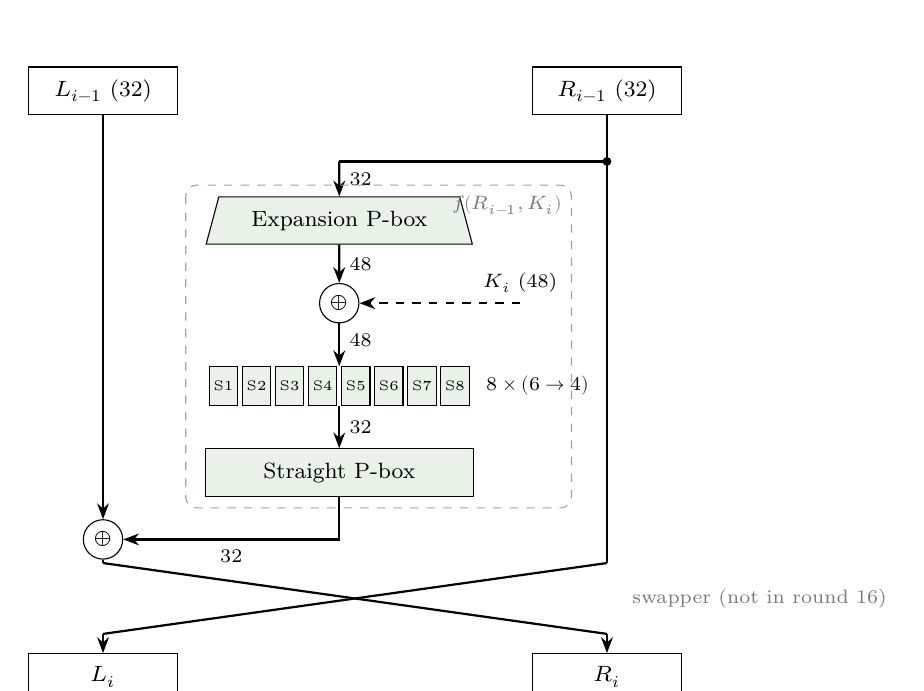
\begin{tikzpicture}[font=\footnotesize,x=1cm,y=1cm,hb/.style={draw,minimum width=1.9cm,minimum height=6mm},
  fb/.style={draw,fill=green!10,minimum width=3.4cm,minimum height=6mm,align=center}]
  \node[hb] (L) at (0,0) {$L_{i-1}$ (32)};
  \node[hb] (R) at (6.4,0) {$R_{i-1}$ (32)};
  \draw[thick] (R) -- (6.4,-6.0);
  \fill (6.4,-0.9) circle (1.6pt);
  \draw[thick] (6.4,-0.9) -- (3,-0.9);
  \node[fb,trapezium,trapezium angle=75,minimum width=2.6cm] (E) at (3,-1.65) {Expansion P-box};
  \draw[arr] (3,-0.9) -- node[right,font=\scriptsize]{32} (E);
  \node[draw,circle,inner sep=0pt,minimum size=5mm] (X) at (3,-2.7) {$\oplus$};
  \draw[arr] (E) -- node[right,font=\scriptsize]{48} (X);
  \draw[arr,dashed] (5.3,-2.7) node[above,font=\scriptsize]{$K_i$ (48)} -- (X);
  \foreach \j in {1,...,8} \node[draw,fill=green!10,minimum width=3.6mm,minimum height=5mm,inner sep=0pt,font=\tiny] (S\j) at (3+0.42*\j-1.89,-3.75) {S\j};
  \draw[arr] (X) -- node[right,font=\scriptsize,pos=0.4]{48} (3,-3.5);
  \node[font=\scriptsize,anchor=west] at (4.75,-3.75) {$8 \times (6 \to 4)$};
  \node[fb] (P) at (3,-4.85) {Straight P-box};
  \draw[arr] (3,-4.0) -- node[right,font=\scriptsize]{32} (P);
  \draw[gray,dashed,rounded corners] (1.05,-1.2) rectangle (5.95,-5.3);
  \node[gray!60!black,anchor=north east,font=\scriptsize] at (5.95,-1.2) {$f(R_{i-1}, K_i)$};
  \node[draw,circle,inner sep=0pt,minimum size=5mm] (M) at (0,-5.7) {$\oplus$};
  \draw[arr] (L) -- (M);
  \draw[arr] (P.south) |- node[pos=0.75,below,font=\scriptsize]{32} (M.east);
  \draw[thick] (M) -- (0,-6.0);
  \draw[thick] (0,-6.0) -- (6.4,-6.9); \draw[thick] (6.4,-6.0) -- (0,-6.9);
  \node[gray!60!black,font=\scriptsize,anchor=west] at (6.6,-6.45) {swapper (not in round 16)};
  \node[hb] (L2) at (0,-7.45) {$L_i$};
  \node[hb] (R2) at (6.4,-7.45) {$R_i$};
  \draw[arr] (0,-6.9) -- (L2); \draw[arr] (6.4,-6.9) -- (R2);
\end{tikzpicture}
\end{center}
Inside $f$: the expansion P-box widens $R_{i-1}$ from 32 to 48 bits, the whitener XORs in $K_i$, eight S-boxes reduce 48 bits to 32 (row $=$ outer bits, column $=$ middle 4 bits), and a straight P-box permutes the 32 bits.

\textbf{Pseudocode} (Forouzan style; bit arrays are indexed from 1).

\begin{minipage}[t]{0.49\linewidth}\small
\textbf{substitute} (inBlock[48], outBlock[32], \emph{SubstitutionTables}[8, 4, 16])\\
\{\\
\hspace*{1em}\textbf{for} ($i = 1$ to 8)\\
\hspace*{1em}\{\\
\hspace*{2em}$b \leftarrow (i - 1) \times 6$ \hfill // start of group $i$\\
\hspace*{2em}row $\leftarrow 2 \times$ inBlock[$b{+}1$] $+$ inBlock[$b{+}6$]\\
\hspace*{2em}col $\leftarrow 8 \times$ inBlock[$b{+}2$] $+ \ 4 \times$ inBlock[$b{+}3$]\\
\hspace*{4.5em}$+\ 2 \times$ inBlock[$b{+}4$] $+$ inBlock[$b{+}5$]\\
\hspace*{2em}value $\leftarrow$ \emph{SubstitutionTables}[$i$][row][col]\\
\hspace*{2em}$o \leftarrow (i - 1) \times 4$\\
\hspace*{2em}outBlock[$o{+}1$] $\leftarrow$ value / 8;\ \ value $\leftarrow$ value mod 8\\
\hspace*{2em}outBlock[$o{+}2$] $\leftarrow$ value / 4;\ \ value $\leftarrow$ value mod 4\\
\hspace*{2em}outBlock[$o{+}3$] $\leftarrow$ value / 2;\ \ value $\leftarrow$ value mod 2\\
\hspace*{2em}outBlock[$o{+}4$] $\leftarrow$ value\\
\hspace*{1em}\}\\
\}
\end{minipage}\hfill
\begin{minipage}[t]{0.47\linewidth}\small
\textbf{Key\_Generator} (keyWithParities[64], RoundKeys[16, 48], \emph{ShiftTable}[16])\\
\{\\
\hspace*{1em}\textbf{permute} (64, 56, keyWithParities, cipherKey, \emph{ParityDropTable})\\
\hspace*{1em}\textbf{split} (56, 28, cipherKey, leftKey, rightKey)\\
\hspace*{1em}\textbf{for} (round $= 1$ to 16)\\
\hspace*{1em}\{\\
\hspace*{2em}\textbf{shiftLeft} (leftKey, \emph{ShiftTable}[round])\\
\hspace*{2em}\textbf{shiftLeft} (rightKey, \emph{ShiftTable}[round])\\
\hspace*{2em}\textbf{combine} (28, 56, leftKey, rightKey, preRoundKey)\\
\hspace*{2em}\textbf{permute} (56, 48, preRoundKey, RoundKeys[round], \emph{KeyCompressionTable})\\
\hspace*{1em}\}\\
\}\\[2pt]
\emph{ShiftTable} $= [1, 1, 2, 2, 2, 2, 2, 2, 1, 2, 2, 2, 2, 2, 2, 1]$; shiftLeft is a circular left shift of a 28-bit half.
\end{minipage}

\medskip
\emph{Check:} the substitute routine reproduces the S-box output \ttx{8AFE657E} of the round trace above (tested by script).
\end{worked}

\begin{mustknow}[: DES at a glance]
64-bit block, 56-bit key (64 with parity), 16 Feistel rounds, 48-bit round keys. Round: $L_i = R_{i-1}$, $R_i = L_{i-1} \oplus f(R_{i-1}, K_i)$, no swap in round 16. $f$: expansion 32 $\to$ 48, XOR $K_i$, 8 S-boxes $6 \to 4$ (row $= b_1 b_6$, column $= b_2..b_5$), straight P-box 32 $\to$ 32. Keys: parity drop 64 $\to$ 56, split 28 $+$ 28, rotate left 1 bit in rounds 1, 2, 9, 16 and 2 bits otherwise, compression 56 $\to$ 48. Decryption: same algorithm, keys $K_{16}..K_1$.
\end{mustknow}

\subsection{DES analysis: avalanche and completeness}
Two properties are expected of a good block cipher. The \textbf{avalanche effect} means that a small change in the plaintext (or the key) should change many ciphertext bits, about half of them. \textbf{Completeness} means that each ciphertext bit should depend on many plaintext bits. In DES both come from the combination of S-boxes (confusion) and P-boxes, including the expansion that feeds each edge bit to two S-boxes (diffusion), and tests show DES is strong in both.

\begin{worked}[: avalanche in DES (Forouzan's example)]
\textbf{Q.} Encrypt the plaintexts \ttx{0000000000000000} and \ttx{0000000000000001} (differing in one bit) with the key \ttx{22234512987ABB23}. How many ciphertext bits differ?

\textbf{A.} The ciphertexts are \ttx{4789FD476E82A5F1} and \ttx{0A4ED5C15A63FEA3}; their XOR has \textbf{29} one-bits, so a 1-bit change of the plaintext changed 29 of the 64 ciphertext bits. The number of differing bits after each round (script) shows how fast the difference spreads:
\begin{center}\small\setlength{\tabcolsep}{3.4pt}
\begin{tabular}{@{}l*{16}{c}@{}}
\toprule
round & 1&2&3&4&5&6&7&8&9&10&11&12&13&14&15&16\\
\midrule
bits differing & 1&6&20&29&30&33&32&29&32&39&33&28&30&31&30&29\\
\bottomrule
\end{tabular}
\end{center}
After only 3 to 4 rounds the difference is already near the ideal of 32; the remaining rounds keep it there.
\end{worked}

\subsection{Weaknesses of DES}
\textbf{Design of the S-boxes and P-boxes.} Critics point out a few irregularities, none of which has led to a practical attack:
\begin{itemize}
  \item In S-box 4, the last three output bits can be derived in the same way as the first output bit by complementing some of the input bits.
  \item Two specially chosen inputs to the S-box array can produce the same output.
  \item The same output of a single round can be obtained by changing bits in only three neighbouring S-boxes.
  \item The initial and final permutations have no security benefit, and in the expansion P-box the first and fourth bits of every 4-bit section are repeated.
\end{itemize}

\textbf{Key size.} The real weakness is the 56-bit key. A brute-force attack on one ciphertext block must try up to $2^{56} \approx 7.2 \times 10^{16}$ keys. At $10^6$ keys per second on each of $10^6$ parallel chips, i.e.\ $10^{12}$ keys per second, the whole key space takes $2^{56}/10^{12} \approx 72\,058$ seconds $\approx$ \textbf{20 hours} (10 hours on average, since the key is found halfway on average). Networked computers simulate parallel hardware: the slides quote 3500 Internet computers finding an RSA Laboratories challenge key in 120 days, so 42\,000 machines would need $3500 \times 120 / 42\,000 = 10$ days.

\textbf{Weak keys.} A \textbf{weak key} is one for which all 16 round keys are the same. This happens when, after the parity drop, each 28-bit half is all 0s or all 1s, because rotating such a half changes nothing. There are 4 weak keys (verified by script: each gives a single distinct round key):
\begin{center}\small
\begin{tabular}{@{}ll@{}}
\toprule
Key before parity drop (64 bits) & Actual key: $C_0$, $D_0$ (hex)\\
\midrule
\ttx{0101 0101 0101 0101} & \ttx{0000000} \ttx{0000000}\\
\ttx{1F1F 1F1F 0E0E 0E0E} & \ttx{0000000} \ttx{FFFFFFF}\\
\ttx{E0E0 E0E0 F1F1 F1F1} & \ttx{FFFFFFF} \ttx{0000000}\\
\ttx{FEFE FEFE FEFE FEFE} & \ttx{FFFFFFF} \ttx{FFFFFFF}\\
\bottomrule
\end{tabular}
\end{center}
With all round keys equal, the key order $K_{16}, \dots, K_1$ is the same as $K_1, \dots, K_{16}$, so the reverse cipher \emph{is} the cipher: \imp{encrypting twice with a weak key returns the plaintext}, $E_K(E_K(P)) = P$.

\textbf{Semi-weak keys.} A \textbf{semi-weak key} creates only 2 distinct round keys, each used 8 times (each half follows the alternating pattern $0101\dots$ or $1010\dots$, or is constant, with at least one half alternating). They come in \textbf{6 pairs} $(k_1, k_2)$ whose round-key sequences are each other's reverse, so $E_{k_2}(E_{k_1}(P)) = P$: one key of the pair decrypts what the other encrypts. The pairs (all checked by script) are:
\begin{center}\small
\begin{tabular}{@{}ll@{\hspace{2.5em}}ll@{}}
\toprule
First key & Second key & First key & Second key\\
\midrule
\ttx{01FE 01FE 01FE 01FE} & \ttx{FE01 FE01 FE01 FE01} & \ttx{1FFE 1FFE 0EFE 0EFE} & \ttx{FE1F FE1F FE0E FE0E}\\
\ttx{1FE0 1FE0 0EF1 0EF1} & \ttx{E01F E01F F10E F10E} & \ttx{011F 011F 010E 010E} & \ttx{1F01 1F01 0E01 0E01}\\
\ttx{01E0 01E0 01F1 01F1} & \ttx{E001 E001 F101 F101} & \ttx{E0FE E0FE F1FE F1FE} & \ttx{FEE0 FEE0 FEF1 FEF1}\\
\bottomrule
\end{tabular}
\end{center}

\textbf{Possible weak keys.} Forouzan lists \textbf{48 possible weak keys}, which create only 4 distinct round keys, each used 4 times (halves repeating with period 4, such as $0011\,0011\dots$). Since $2^{56}$ keys contain only $4 + 12 + 48 = 64$ such keys, a randomly chosen key is weak with probability $2^{-50}$, so these keys matter only if they are chosen on purpose.

\textbf{Key complement.} Let $\bar{x}$ be the bitwise complement. Then $E_{\bar K}(\bar P) = \overline{E_K(P)}$. Proof: complementing $K$ complements every round key, and complementing the data complements $R_{i-1}$ and hence its expansion; then $E(\bar R) \oplus \bar K_i = E(R) \oplus K_i$, so the S-box inputs and $f$ are unchanged, and $\bar L \oplus f = \overline{L \oplus f}$, so every half stays complemented through all rounds (checked by script). As a result, a chosen-plaintext attacker who has $C_1 = E_K(P)$ and $C_2 = E_K(\bar P)$ can test two keys with one encryption ($K$ and $\bar K$), halving the brute-force work to $2^{55}$.

\subsection{Multiple DES}
The obvious fix for a short key is to encrypt several times with different keys. This only helps because DES is \textbf{not a group}: if for every $K_1$, $K_2$ there were a $K_3$ with $E_{K_2}(E_{K_1}(P)) = E_{K_3}(P)$, double encryption would just be single DES with another key. It has been shown that no such $K_3$ exists in general, so cascading DES really produces new mappings.

\textbf{Double DES.} $C = E_{K_2}(E_{K_1}(P))$ and $P = D_{K_1}(D_{K_2}(C))$, with a 112-bit key $(K_1, K_2)$. One would expect $2^{112}$ trials for a brute-force attack, but the \textbf{meet-in-the-middle attack} (a known-plaintext attack) needs only about $2^{57}$. The derivation starts from the middle text $M$, the value between the two encryptions:
\[
M = E_{K_1}(P) \quad\text{and also}\quad M = D_{K_2}(C).
\]
Given one known pair $(P, C)$, Eve encrypts $P$ under all $2^{56}$ values of $K_1$ and stores the results $M$ in a table sorted by $M$. She then decrypts $C$ under all $2^{56}$ values of $K_2$ and looks up each $D_{K_2}(C)$ in the table. Every match gives a candidate pair $(K_1, K_2)$, since it makes both equations hold. The cost is $2^{56} + 2^{56} = 2^{57}$ DES operations (plus memory for $2^{56}$ entries), instead of $2^{56} \times 2^{56} = 2^{112}$, because the two keys are searched \emph{one after the other} rather than in all combinations. Some matches are false: $2^{112}$ key pairs map to only $2^{64}$ middle values, so about $2^{112}/2^{64} = 2^{48}$ pairs fit one $(P, C)$ by chance; testing the candidates on a second known pair $(P', C')$ leaves about $2^{48}/2^{64} < 1$ false survivor, so the right key is identified. \imp{Double DES raises the work only from $2^{56}$ to $2^{57}$, not to $2^{112}$.}

\textbf{Triple DES with two keys.} $C = E_{K_1}(D_{K_2}(E_{K_1}(P)))$ and $P = D_{K_1}(E_{K_2}(D_{K_1}(C)))$, the \textbf{EDE} (encrypt--decrypt--encrypt) form. The key is 112 bits, and a meet-in-the-middle attack now has to split three stages into one and two, which leaves a $2^{112}$ search on one side, so the attack no longer helps. The middle stage is a \emph{decryption} for compatibility: with $K_1 = K_2$ the first two stages cancel and 3DES becomes single DES, so a 3DES device can talk to an old DES device (checked by script). Two-key 3DES is used in PEM and in the financial standard ANS X9.17 / ISO 8732.

\textbf{Triple DES with three keys.} $C = E_{K_3}(D_{K_2}(E_{K_1}(P)))$ with a 168-bit key. Meet-in-the-middle reduces its effective strength to about $2^{112}$, which is still far beyond brute force; it is used in PGP and S/MIME.

\subsection{Security of DES in one line each}
\begin{itemize}
  \item \textbf{Brute force:} $2^{56}$ keys ($2^{55}$ with the complement property), feasible with special hardware or networked computers.
  \item \textbf{Differential cryptanalysis:} DES can be broken with $2^{47}$ chosen plaintexts; its S-boxes were evidently designed against this attack, which is why it is no better than brute force in practice.
  \item \textbf{Linear cryptanalysis:} DES can be broken with $2^{43}$ known plaintexts, a newer attack the designers did not anticipate.
\end{itemize}

\begin{fixbox}
\begin{itemize}
  \item The slides' \textbf{substitute} pseudocode (L8 slide 16, as in Forouzan) declares inBlock[32], outBlock[48]; the sizes are swapped (48 bits in, 32 bits out). It also indexes inBlock[$i \times 6 + 1$] with $i = 1..8$, which reaches position 49 for $i = 8$; the group offset must be $(i - 1) \times 6$ (and $(i - 1) \times 4$ for outBlock), as in the corrected version in the Q6 answer (verified by script).
  \item Semi-weak key table (L8 slide 23), row 3: \ttx{01E0 01E1 01F1 01F1} should be \ttx{01E0 01E0 01F1 01F1}. \ttx{E1} differs from \ttx{E0} only in the parity bit, so it is the same 56-bit key, but it violates odd parity.
  \item Key-size slide (L8 slide 21): ``In 1977 a team of researchers used 3500 computers \dots\ RSA Laboratories'' should read 1997 (RSA's DES Challenge); DES itself was only published in 1977.
\end{itemize}
\end{fixbox}

% College Lecture 9: AES (Forouzan ch. 7, Stallings ch. 5). Every byte in this file (S-box, SubBytes, ShiftRows,
% MixColumns, AddRoundKey, key expansion, FIPS-197 Appendix B round 1 and ciphertext) recomputed by
% scratchpad/aes/aes_check.py and extra.py; the S-box is generated from GF(2^8) inverse + affine map and matched to FIPS-197.
\providecommand{\aesM}[1]{\left(\begin{tabular}{@{\hspace{2pt}}>{\ttfamily}c@{\hspace{5pt}}>{\ttfamily}c@{\hspace{5pt}}>{\ttfamily}c@{\hspace{5pt}}>{\ttfamily}c@{\hspace{2pt}}}#1\end{tabular}\right)}
\providecommand{\aesB}[1]{\textcolor{acc}{\textbf{#1}}}

\section{Advanced Encryption Standard (AES)}\label{sec:aes}

\textbf{Why DES had to be replaced.} By the late 1990s the 56-bit DES key was within reach of brute force: a $2^{56}$ search is about $7.2 \times 10^{16}$ trials, and a purpose-built machine (EFF, 1998) found a DES key in a few days. Triple DES fixes the key length but runs three DES encryptions per block, which is slow in software, and it keeps DES's 64-bit block, which is too small for encrypting large volumes of data under one key. NIST therefore ran an open competition, judged on three criteria (\emph{security, cost, implementation}), and in 2000 chose \textbf{Rijndael} by Daemen and Rijmen. It was published as the \textbf{Advanced Encryption Standard} (FIPS 197) in December 2001.

\textbf{What kind of cipher it is.} \imp{AES is a symmetric-key, non-Feistel block cipher that encrypts 128-bit blocks with a 128-, 192- or 256-bit key in 10, 12 or 14 rounds.} Non-Feistel means that, unlike DES, the round does not split the block into halves and hide a one-way function inside a swap. Instead every step of the round is itself invertible, and decryption runs the inverse steps in reverse order. Such a design is called a substitution--permutation network: substitution (SubBytes) gives confusion, and permutation plus mixing (ShiftRows, MixColumns) give diffusion.

\subsection{Parameters and data units}
The block is always 128 bits and every round key is always 128 bits, whatever the cipher-key length. Only the number of rounds $N_r$ depends on the key size, because a longer key needs more rounds before every key bit has influenced every state bit. Since one round key is added before round 1 and one in each of the $N_r$ rounds, \imp{the number of round keys is $N_r + 1$}, and each round key is 4 words.
\begin{center}\small
\begin{tabular}{@{}lccccc@{}}
\toprule
Version & Key (bits) & Rounds $N_r$ & Round keys $N_r + 1$ & Key words $4(N_r + 1)$ & Brute force\\
\midrule
AES-128 & 128 & 10 & 11 & 44 ($w_0$--$w_{43}$) & $2^{128}$\\
AES-192 & 192 & 12 & 13 & 52 ($w_0$--$w_{51}$) & $2^{192}$\\
AES-256 & 256 & 14 & 15 & 60 ($w_0$--$w_{59}$) & $2^{256}$\\
\bottomrule
\end{tabular}
\end{center}

\textbf{Data units.} AES names five units. A \emph{bit} is a binary digit; a \emph{byte} is 8 bits and is treated as an element of GF$(2^8)$, written as two hex digits; a \emph{word} is 4 bytes (32 bits), seen either as a row or as a column of 4 bytes; a \emph{block} is 16 bytes (128 bits), $b_0 b_1 \dots b_{15}$; and the \emph{state} is the block arranged as a $4 \times 4$ matrix of bytes $s_{r,c}$, which is what every transformation actually acts on. Each column of the state is one word, so the state is also four words $w_0 w_1 w_2 w_3$ side by side.

\textbf{Block to state.} The 16 bytes fill the state \textbf{column by column}: bytes $b_0..b_3$ form column 0 (top to bottom), $b_4..b_7$ column 1, and so on, so that
\[
s_{r,c} = b_{r + 4c}, \qquad\text{equivalently}\qquad b_i \to s_{\,i \bmod 4,\; \lfloor i/4 \rfloor}.
\]
The reverse mapping reads the state column by column to get the output block. This column-major order matters because MixColumns and AddRoundKey work on columns, so four consecutive input bytes are processed together.

\begin{trap}[: filling the state row-wise]
Writing the 16 bytes \emph{across} the rows is the most common slip. The first four bytes go \emph{down} column 0. With the wrong order every later step (ShiftRows, MixColumns, the key words as columns) gives a wrong answer.
\end{trap}

\begin{worked}[: text block to state (slide Example 1, from Forouzan)]
\textbf{Q.} Show the state for the text block ``AES uses a matrix'', letters coded A $= 00$ to Z $= 25$ in hex, padding with Z.\\[2pt]
\textbf{A.} Removing spaces gives 14 letters, so two bogus Z's make 16: \ttx{AESUSESAMATRIXZZ}. Each letter's number is written in \textbf{hex} (for example M $= 12 = $ \ttx{0C}, R $= 17 = $ \ttx{11}, X $= 23 = $ \ttx{17}, Z $= 25 = $ \ttx{19}):
\begin{center}\small\ttfamily\setlength{\tabcolsep}{3.2pt}
\begin{tabular}{@{}l*{16}{c}@{}}
\rmfamily Text & A&E&S&U&S&E&S&A&M&A&T&R&I&X&Z&Z\\
\rmfamily Hex  & 00&04&12&14&12&04&12&00&0C&00&13&11&08&17&19&19
\end{tabular}
\end{center}
Filling column by column (first four bytes down column 0):
\[
\text{State} = \aesM{00&12&0C&08\\04&04&00&17\\12&12&13&19\\14&00&11&19}
\]
Check: $s_{1,3} = b_{1 + 12} = b_{13} = $ \ttx{17} (the X). The slide prints \ttx{23} here; see the corrections box.
\end{worked}

\subsection{Round structure}
Encryption of AES-128 is one key addition followed by 10 rounds:
\begin{enumerate}
  \item \textbf{Pre-round:} AddRoundKey with round key $K_0 = w_0..w_3$ (the cipher key itself).
  \item \textbf{Rounds 1 to $N_r - 1$:} SubBytes, ShiftRows, MixColumns, AddRoundKey (with $K_i = w_{4i}..w_{4i+3}$).
  \item \textbf{Last round $N_r$:} SubBytes, ShiftRows, AddRoundKey, \textbf{without MixColumns}.
\end{enumerate}

\begin{center}
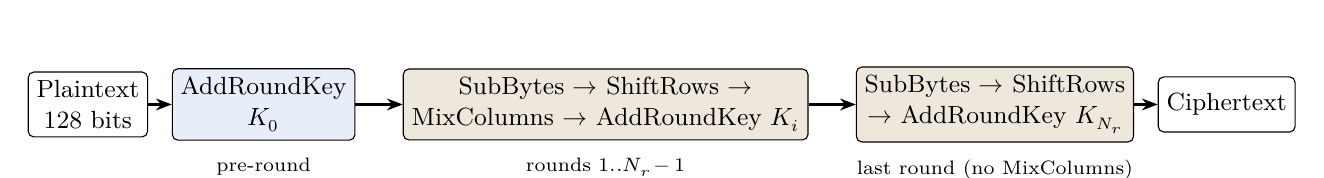
\begin{tikzpicture}[node distance=3mm, every node/.style={font=\footnotesize}]
\node[box] (p) {Plaintext\\128 bits};
\node[box, right=of p, fill=acc!10] (k0) {AddRoundKey\\$K_0$};
\node[box, right=6mm of k0, fill=orange!12] (r) {SubBytes $\to$ ShiftRows $\to$\\MixColumns $\to$ AddRoundKey $K_i$};
\node[box, right=6mm of r, fill=orange!12] (l) {SubBytes $\to$ ShiftRows\\$\to$ AddRoundKey $K_{N_r}$};
\node[box, right=of l] (c) {Ciphertext};
\draw[arr] (p) -- (k0); \draw[arr] (k0) -- (r); \draw[arr] (r) -- (l); \draw[arr] (l) -- (c);
\node[below=1mm of r, font=\scriptsize] {rounds $1..N_r - 1$};
\node[below=1mm of l, font=\scriptsize] {last round (no MixColumns)};
\node[below=1mm of k0, font=\scriptsize] {pre-round};
\end{tikzpicture}
\end{center}

\textbf{Why a key addition comes first.} Every step except AddRoundKey is public and keyless. If the cipher began with SubBytes, an attacker who knows the plaintext could compute that step himself, so it would add work but no secrecy. Adding the key first (key whitening) means that from the very first non-linear step onward, nothing is computable without the key.

\textbf{Why the last round has no MixColumns.} MixColumns is linear over GF$(2^8)$, so $\mathrm{MC}(Y) \oplus K = \mathrm{MC}\big(Y \oplus \mathrm{MC}^{-1}(K)\big)$. If the last round ended with MixColumns and then AddRoundKey, an attacker could apply InvMixColumns to the ciphertext and obtain $Y \oplus \mathrm{MC}^{-1}(K_{N_r})$, which is just the same cipher without the final MixColumns under a different (equally unknown) key. The final MixColumns therefore adds no security. Leaving it out costs nothing and makes the decryption algorithm have the same shape as encryption, which allows the ``equivalent inverse cipher'' to reuse the same hardware.

\begin{mustknow}
AES: block 128, key 128/192/256, rounds 10/12/14, round keys $N_r + 1$ (always 128 bits each), $4(N_r + 1)$ words. Pre-round AddRoundKey; rounds 1..$N_r - 1$: \textbf{SubBytes, ShiftRows, MixColumns, AddRoundKey}; last round drops MixColumns. The state is filled \textbf{column by column}, $s_{r,c} = b_{r + 4c}$.
\end{mustknow}

\subsection{SubBytes (substitution) \hot}
\likely{``Find SubBytes of \ttx{0x53}'' or ``apply SubBytes to the given state using the S-box''; or derive one S-box entry from the GF$(2^8)$ inverse and the affine transform.}

\textbf{Problem and idea.} A cipher built only from XORs, shifts and matrix multiplications is linear, and a linear cipher falls to solving a system of equations. SubBytes is the one non-linear step in AES. Each of the 16 bytes is replaced independently by looking it up in one fixed $16 \times 16$ table, the S-box. Because the same table is used for every byte, \imp{equal input bytes always give equal output bytes}; SubBytes is an \emph{intrabyte} transformation, since a byte's output depends on that byte alone.

\textbf{Lookup rule.} Write the byte as two hex digits $xy$. The \textbf{left digit $x$ selects the row} and the \textbf{right digit $y$ selects the column}; the entry there is the output. For example \ttx{53}: row 5, column 3 gives \ttx{ED}, and \ttx{00}: row 0, column 0 gives \ttx{63}.

\begin{center}
\small\ttfamily\setlength{\tabcolsep}{4pt}\renewcommand{\arraystretch}{1.05}
\begin{tabular}{@{}>{\columncolor{acc!10}}c|*{16}{c}@{}}
\rowcolor{acc!10}$x\backslash y$ & \textbf{0}&\textbf{1}&\textbf{2}&\textbf{3}&\textbf{4}&\textbf{5}&\textbf{6}&\textbf{7}&\textbf{8}&\textbf{9}&\textbf{A}&\textbf{B}&\textbf{C}&\textbf{D}&\textbf{E}&\textbf{F}\\\hline
\textbf{0} & 63 & 7C & 77 & 7B & F2 & 6B & 6F & C5 & 30 & 01 & 67 & 2B & FE & D7 & AB & 76\\
\textbf{1} & CA & 82 & C9 & 7D & FA & 59 & 47 & F0 & AD & D4 & A2 & AF & 9C & A4 & 72 & C0\\
\textbf{2} & B7 & FD & 93 & 26 & 36 & 3F & F7 & CC & 34 & A5 & E5 & F1 & 71 & D8 & 31 & 15\\
\textbf{3} & 04 & C7 & 23 & C3 & 18 & 96 & 05 & 9A & 07 & 12 & 80 & E2 & EB & 27 & B2 & 75\\
\textbf{4} & 09 & 83 & 2C & 1A & 1B & 6E & 5A & A0 & 52 & 3B & D6 & B3 & 29 & E3 & 2F & 84\\
\textbf{5} & 53 & D1 & 00 & ED & 20 & FC & B1 & 5B & 6A & CB & BE & 39 & 4A & 4C & 58 & CF\\
\textbf{6} & D0 & EF & AA & FB & 43 & 4D & 33 & 85 & 45 & F9 & 02 & 7F & 50 & 3C & 9F & A8\\
\textbf{7} & 51 & A3 & 40 & 8F & 92 & 9D & 38 & F5 & BC & B6 & DA & 21 & 10 & FF & F3 & D2\\
\textbf{8} & CD & 0C & 13 & EC & 5F & 97 & 44 & 17 & C4 & A7 & 7E & 3D & 64 & 5D & 19 & 73\\
\textbf{9} & 60 & 81 & 4F & DC & 22 & 2A & 90 & 88 & 46 & EE & B8 & 14 & DE & 5E & 0B & DB\\
\textbf{A} & E0 & 32 & 3A & 0A & 49 & 06 & 24 & 5C & C2 & D3 & AC & 62 & 91 & 95 & E4 & 79\\
\textbf{B} & E7 & C8 & 37 & 6D & 8D & D5 & 4E & A9 & 6C & 56 & F4 & EA & 65 & 7A & AE & 08\\
\textbf{C} & BA & 78 & 25 & 2E & 1C & A6 & B4 & C6 & E8 & DD & 74 & 1F & 4B & BD & 8B & 8A\\
\textbf{D} & 70 & 3E & B5 & 66 & 48 & 03 & F6 & 0E & 61 & 35 & 57 & B9 & 86 & C1 & 1D & 9E\\
\textbf{E} & E1 & F8 & 98 & 11 & 69 & D9 & 8E & 94 & 9B & 1E & 87 & E9 & CE & 55 & 28 & DF\\
\textbf{F} & 8C & A1 & 89 & 0D & BF & E6 & 42 & 68 & 41 & 99 & 2D & 0F & B0 & 54 & BB & 16\\
\end{tabular}\\[2pt]
\rmfamily\small AES S-box (FIPS-197), generated by script from the definition below and checked entry by entry.
\end{center}

\textbf{How the S-box is built.} The table is not arbitrary; each entry is computed in two steps from the byte $a$ viewed as a polynomial in GF$(2^8)$ with modulus $m(x) = x^8 + x^4 + x^3 + x + 1$ (\ttx{11B}).
\begin{enumerate}
  \item \textbf{Multiplicative inverse:} $b = a^{-1}$ in GF$(2^8)$, with \ttx{00} mapped to \ttx{00} (it has no inverse). The inverse map is highly non-linear, which is what resists linear and differential cryptanalysis. This is why AES works in GF$(2^8)$ and not in $\mathbb{Z}_{256}$: in $\mathbb{Z}_{256}$ every even byte lacks an inverse, so the map would not be a permutation.
  \item \textbf{Affine transformation over GF(2):} with $c = \ttx{63} = 0110\,0011$,
  \[
  b'_i = b_i \oplus b_{(i+4) \bmod 8} \oplus b_{(i+5) \bmod 8} \oplus b_{(i+6) \bmod 8} \oplus b_{(i+7) \bmod 8} \oplus c_i, \qquad i = 0..7 .
  \]
  This step breaks the simple algebraic form $a \mapsto a^{-1}$ and removes its fixed points ($00 \mapsto 00$ and $01 \mapsto 01$). As a result the AES S-box has no fixed point ($S(a) \ne a$ for all 256 bytes) and none with $S(a) = \bar{a}$.
\end{enumerate}
InvSubBytes uses the inverse table: undo the affine map, then take the GF$(2^8)$ inverse. Without that table, find the output in the S-box and read off its row and column (for example \ttx{ED} sits at row 5, column 3, so InvSubBytes(\ttx{ED}) $=$ \ttx{53}).

\begin{worked}[: one S-box entry from the definition]
\textbf{Q.} Show that SubBytes(\ttx{53}) $=$ \ttx{ED} by computing it, not by looking it up.\\[2pt]
\textbf{A.} \emph{Step 1.} $\ttx{53} = x^6 + x^4 + x + 1$. Its inverse modulo $m(x)$, by the extended Euclidean algorithm in GF$(2^8)$, is $\ttx{CA} = x^7 + x^6 + x^3 + x$ (check: $\ttx{53} \cdot \ttx{CA} = \ttx{01}$). So $b = \ttx{CA} = 1100\,1010$, that is $b_7..b_0 = 1,1,0,0,1,0,1,0$.\\
\emph{Step 2.} Apply $b'_i = b_i \oplus b_{i+4} \oplus b_{i+5} \oplus b_{i+6} \oplus b_{i+7} \oplus c_i$ (indices mod 8, $c = \ttx{63}$, so $c_0 = c_1 = c_5 = c_6 = 1$):
\begin{center}\small\setlength{\tabcolsep}{5pt}
\begin{tabular}{@{}c|cccccc|c@{}}
\toprule
$i$ & $b_i$ & $b_{i+4}$ & $b_{i+5}$ & $b_{i+6}$ & $b_{i+7}$ & $c_i$ & $b'_i$\\
\midrule
0 & 0 & 0 & 0 & 1 & 1 & 1 & \textbf{1}\\
1 & 1 & 0 & 1 & 1 & 0 & 1 & \textbf{0}\\
2 & 0 & 1 & 1 & 0 & 1 & 0 & \textbf{1}\\
3 & 1 & 1 & 0 & 1 & 0 & 0 & \textbf{1}\\
4 & 0 & 0 & 1 & 0 & 1 & 0 & \textbf{0}\\
5 & 0 & 1 & 0 & 1 & 0 & 1 & \textbf{1}\\
6 & 1 & 0 & 1 & 0 & 0 & 1 & \textbf{1}\\
7 & 1 & 1 & 0 & 0 & 1 & 0 & \textbf{1}\\
\bottomrule
\end{tabular}
\end{center}
Reading $b'_7..b'_0 = 1110\,1101$ gives \textbf{SubBytes(\ttx{53}) $=$ \ttx{ED}}, which matches row 5, column 3 of the table.
\end{worked}

\begin{worked}[: SubBytes of a state (slide Example 2)]
\textbf{Q.} Apply SubBytes to the state of Example 1.\\[2pt]
\textbf{A.} Each byte is looked up independently (row $=$ left digit, column $=$ right digit): \ttx{00}$\to$\ttx{63}, \ttx{04}$\to$\ttx{F2}, \ttx{12}$\to$\ttx{C9}, \ttx{14}$\to$\ttx{FA}, \ttx{0C}$\to$\ttx{FE}, \ttx{13}$\to$\ttx{7D}, \ttx{11}$\to$\ttx{82}, \ttx{08}$\to$\ttx{30}, \ttx{17}$\to$\ttx{F0}, \ttx{19}$\to$\ttx{D4}.
\[
\aesM{00&12&0C&08\\04&04&00&17\\12&12&13&19\\14&00&11&19}
\xrightarrow{\ \text{SubBytes}\ }
\aesM{63&C9&FE&30\\F2&F2&63&\aesB{F0}\\C9&C9&7D&D4\\FA&63&82&D4}
\]
The two \ttx{04}'s in row 1 both become \ttx{F2}, showing that SubBytes alone does not hide repeated bytes; ShiftRows and MixColumns are needed for that.
\end{worked}
Single-bit changes spread: \ttx{5A} and \ttx{5B} differ in one bit, but $S(\ttx{5A}) = \ttx{BE}$ and $S(\ttx{5B}) = \ttx{39}$ differ in four bits ($\ttx{BE} \oplus \ttx{39} = \ttx{87} = 1000\,0111$).

\subsection{ShiftRows (permutation) \hot}
\asked{2025--26 Q4(a) (part of 6 marks): ShiftRows on a given state. Solved in full after AddRoundKey below.}

\textbf{Problem and idea.} SubBytes changes each byte on its own, and MixColumns (next) mixes only the four bytes inside one column. Without a step that moves bytes \emph{between} columns, the four columns would never interact, and AES would be four independent 32-bit ciphers running side by side, each attackable separately. ShiftRows is that step: it permutes bytes so that each column's four bytes end up in four different columns.

\textbf{Mechanism.} \imp{Row $r$ of the state is rotated cyclically left by $r$ bytes}: row 0 is unchanged, row 1 moves left by 1, row 2 by 2, row 3 by 3. In symbols $s'_{r,c} = s_{r,(c + r) \bmod 4}$. The permutation is at the \emph{byte} level: bytes change position but the bits inside a byte are untouched, unlike DES, whose P-boxes permute single bits. Since the four bytes of input column $c$ lie in rows 0, 1, 2, 3, they are shifted by 0, 1, 2, 3 places and land in four different columns; after the next MixColumns every output column then depends on all four input columns. InvShiftRows rotates row $r$ \emph{right} by $r$ bytes.
\[
\begin{pmatrix}s_{00}&s_{01}&s_{02}&s_{03}\\s_{10}&s_{11}&s_{12}&s_{13}\\s_{20}&s_{21}&s_{22}&s_{23}\\s_{30}&s_{31}&s_{32}&s_{33}\end{pmatrix}
\xrightarrow{\ \text{ShiftRows}\ }
\begin{pmatrix}s_{00}&s_{01}&s_{02}&s_{03}\\s_{11}&s_{12}&s_{13}&s_{10}\\s_{22}&s_{23}&s_{20}&s_{21}\\s_{33}&s_{30}&s_{31}&s_{32}\end{pmatrix}
\]
Applied to the SubBytes output of Example 2 (slide Example 3):
\[
\aesM{63&C9&FE&30\\F2&F2&63&F0\\C9&C9&7D&D4\\FA&63&82&D4}
\xrightarrow{\ \text{ShiftRows}\ }
\aesM{63&C9&FE&30\\F2&63&F0&F2\\7D&D4&C9&C9\\D4&FA&63&82}
\]

\subsection{MixColumns (mixing) \hot}
\likely{``Perform MixColumns on one column'' (one or all four output bytes), or ``show that the given column maps to \dots''.}

\textbf{Problem and idea.} SubBytes is intrabyte and ShiftRows only exchanges bytes, so neither makes a byte depend on its neighbours. MixColumns is the \emph{interbyte} step: it replaces each column by a combination of all four of its bytes, so that changing one input byte changes all four output bytes. To guarantee that each new byte differs from the others even when all four inputs are equal, each input is first multiplied by a different constant and then the products are added. This is a matrix multiplication over GF$(2^8)$, where ``add'' is XOR and ``multiply'' is polynomial multiplication modulo \ttx{11B}:
\[
\begin{pmatrix}s'_{0}\\s'_{1}\\s'_{2}\\s'_{3}\end{pmatrix}
= \aesM{02&03&01&01\\01&02&03&01\\01&01&02&03\\03&01&01&02}
\begin{pmatrix}s_{0}\\s_{1}\\s_{2}\\s_{3}\end{pmatrix},
\qquad
\text{InvMixColumns: } \aesM{0E&0B&0D&09\\09&0E&0B&0D\\0D&09&0E&0B\\0B&0D&09&0E}.
\]
Each row of the matrix is the row above rotated right by one. Written out, $s'_0 = 02 \cdot s_0 \oplus 03 \cdot s_1 \oplus s_2 \oplus s_3$, $s'_1 = s_0 \oplus 02 \cdot s_1 \oplus 03 \cdot s_2 \oplus s_3$, $s'_2 = s_0 \oplus s_1 \oplus 02 \cdot s_2 \oplus 03 \cdot s_3$, $s'_3 = 03 \cdot s_0 \oplus s_1 \oplus s_2 \oplus 02 \cdot s_3$. The two matrices multiply to the identity in GF$(2^8)$ (checked by script), which is why InvMixColumns undoes MixColumns.

\textbf{Why the constants 01, 02, 03.} They make encryption cheap, because multiplying by these needs only a shift and XORs. Multiplying by \ttx{02} is multiplying by $x$: shift the byte left by one bit, and if the bit shifted out (the old top bit $b_7$) was 1, the result has an $x^8$ term, which is reduced by XOR with \ttx{1B} (since $x^8 \equiv x^4 + x^3 + x + 1$). This operation is called \textbf{xtime}. Multiplying by \ttx{03} $= x + 1$ is then $(02 \cdot b) \oplus b$. The matrix is also chosen so that the total number of non-zero bytes in an input column plus its output column is at least 5 (branch number 5), so one changed input byte always changes all four output bytes.
\begin{mustknow}[: xtime]
$02 \cdot b = (b \ll 1)$, then XOR \ttx{1B} if the top bit of $b$ was 1. \qquad $03 \cdot b = (02 \cdot b) \oplus b$. \qquad $01 \cdot b = b$.
\end{mustknow}

\begin{worked}[: one column (FIPS-197 test column)]
\textbf{Q.} Apply MixColumns to the column $(\ttx{DB}, \ttx{13}, \ttx{53}, \ttx{45})^T$.\\[2pt]
\textbf{A.} First the products by 02 and 03 of every input byte:
\begin{center}\small\setlength{\tabcolsep}{5pt}
\begin{tabular}{@{}ccccc@{}}
\toprule
$b$ & binary & shift left & top bit 1? & $02 \cdot b$ \;/\; $03 \cdot b = (02 \cdot b) \oplus b$\\
\midrule
\ttx{DB} & 1101\,1011 & 1011\,0110 $=$ \ttx{B6} & yes: $\ttx{B6} \oplus \ttx{1B}$ & \ttx{AD} \;/\; \ttx{76}\\
\ttx{13} & 0001\,0011 & 0010\,0110 $=$ \ttx{26} & no & \ttx{26} \;/\; \ttx{35}\\
\ttx{53} & 0101\,0011 & 1010\,0110 $=$ \ttx{A6} & no & \ttx{A6} \;/\; \ttx{F5}\\
\ttx{45} & 0100\,0101 & 1000\,1010 $=$ \ttx{8A} & no & \ttx{8A} \;/\; \ttx{CF}\\
\bottomrule
\end{tabular}
\end{center}
Then each output byte is a row of the matrix times the column, XORed left to right:
\begin{align*}
s'_0 &= 02{\cdot}\ttx{DB} \oplus 03{\cdot}\ttx{13} \oplus \ttx{53} \oplus \ttx{45} = \ttx{AD} \oplus \ttx{35} \oplus \ttx{53} \oplus \ttx{45} = \ttx{98} \oplus \ttx{53} \oplus \ttx{45} = \ttx{CB} \oplus \ttx{45} = \textbf{\ttx{8E}}\\
s'_1 &= \ttx{DB} \oplus 02{\cdot}\ttx{13} \oplus 03{\cdot}\ttx{53} \oplus \ttx{45} = \ttx{DB} \oplus \ttx{26} \oplus \ttx{F5} \oplus \ttx{45} = \ttx{FD} \oplus \ttx{F5} \oplus \ttx{45} = \ttx{08} \oplus \ttx{45} = \textbf{\ttx{4D}}\\
s'_2 &= \ttx{DB} \oplus \ttx{13} \oplus 02{\cdot}\ttx{53} \oplus 03{\cdot}\ttx{45} = \ttx{DB} \oplus \ttx{13} \oplus \ttx{A6} \oplus \ttx{CF} = \ttx{C8} \oplus \ttx{A6} \oplus \ttx{CF} = \ttx{6E} \oplus \ttx{CF} = \textbf{\ttx{A1}}\\
s'_3 &= 03{\cdot}\ttx{DB} \oplus \ttx{13} \oplus \ttx{53} \oplus 02{\cdot}\ttx{45} = \ttx{76} \oplus \ttx{13} \oplus \ttx{53} \oplus \ttx{8A} = \ttx{65} \oplus \ttx{53} \oplus \ttx{8A} = \ttx{36} \oplus \ttx{8A} = \textbf{\ttx{BC}}
\end{align*}
Answer: $(\ttx{DB}, \ttx{13}, \ttx{53}, \ttx{45}) \to \mathbf{(\ttx{8E}, \ttx{4D}, \ttx{A1}, \ttx{BC})}$, the FIPS-197 test value. Check: every output byte changed, as the branch-number argument predicts.
\end{worked}

A second check comes from the exam state below: column 0 after ShiftRows is $(\ttx{87}, \ttx{6E}, \ttx{46}, \ttx{A6})$. With $02 \cdot \ttx{87} = \ttx{0E} \oplus \ttx{1B} = \ttx{15}$, $03 \cdot \ttx{6E} = \ttx{DC} \oplus \ttx{6E} = \ttx{B2}$, the first output byte is $\ttx{15} \oplus \ttx{B2} \oplus \ttx{46} \oplus \ttx{A6} = \ttx{47}$, and the whole column becomes $(\ttx{47}, \ttx{37}, \ttx{94}, \ttx{ED})$, which is exactly column 0 of the state given in part (b) of that question (Stallings' figures chain ShiftRows $\to$ MixColumns $\to$ AddRoundKey).

\subsection{AddRoundKey (key adding) \hot}
\asked{2025--26 Q4(b) (part of 6 marks): AddRoundKey of a given state with a given key matrix.}

\textbf{Problem and idea.} The three steps above are fixed and public, so on their own they would be a keyless scrambling that anyone can undo. \imp{AddRoundKey is the only step that uses the key}: it XORs the 128-bit round key into the state. It proceeds column by column, like MixColumns, but where MixColumns multiplies each column by a constant matrix, AddRoundKey \emph{adds} a key word to it: in round $i$, column $c$ becomes $s_c \oplus w_{4i + c}$. Equivalently, write the round key as a $4 \times 4$ matrix whose columns are the four words and XOR the two matrices entry by entry.

\textbf{Inverse.} Addition and subtraction in GF$(2^8)$ are both XOR, and $x \oplus k \oplus k = x$, so AddRoundKey is its own inverse; decryption uses the same operation with the same round key.

\textbf{Doing the XOR by hand.} XOR one hex digit at a time, through its 4-bit binary form: $\ttx{4} \oplus \ttx{A} = 0100 \oplus 1010 = 1110 = \ttx{E}$. Useful shortcuts: $x \oplus x = 0$, $x \oplus 0 = x$, $x \oplus \ttx{F}$ flips all four bits.

\begin{worked}[: 2025--26 Q4 (6 marks), Stallings' AES example]
\textbf{Q.} In AES, the state is given below. (a) Show the ShiftRows transformation. (b) After MixColumns, assume the state and the round key are as given. Perform AddRoundKey.\\[2pt]
\textbf{A.} (a) Row $r$ is rotated left by $r$ bytes: row 0 unchanged; row 1 \ttx{EC 6E 4C 90} $\to$ \ttx{6E 4C 90 EC}; row 2 \ttx{4A C3 46 E7} $\to$ \ttx{46 E7 4A C3}; row 3 \ttx{8C D8 95 A6} $\to$ \ttx{A6 8C D8 95}.
\[
\aesM{87&F2&4D&97\\EC&6E&4C&90\\4A&C3&46&E7\\8C&D8&95&A6}
\xrightarrow{\ \text{ShiftRows}\ }
\aesM{87&F2&4D&97\\\aesB{6E}&\aesB{4C}&\aesB{90}&\aesB{EC}\\\aesB{46}&\aesB{E7}&\aesB{4A}&\aesB{C3}\\\aesB{A6}&\aesB{8C}&\aesB{D8}&\aesB{95}}
\]
(b) AddRoundKey is the byte-wise XOR of the state and the key matrix, $s'_{r,c} = s_{r,c} \oplus k_{r,c}$:
\[
\aesM{47&40&A3&4C\\37&D4&70&9F\\94&E4&3A&42\\ED&A5&A6&BC}
\oplus
\aesM{AC&19&28&57\\77&FA&D1&5C\\66&DC&29&00\\F3&21&41&6A}
=
\aesM{\aesB{EB}&\aesB{59}&\aesB{8B}&\aesB{1B}\\\aesB{40}&\aesB{2E}&\aesB{A1}&\aesB{C3}\\\aesB{F2}&\aesB{38}&\aesB{13}&\aesB{42}\\\aesB{1E}&\aesB{84}&\aesB{E7}&\aesB{D6}}
\]
Working, digit by digit (left digits, then right digits):
\begin{center}\footnotesize\ttfamily\setlength{\tabcolsep}{6pt}
\begin{tabular}{@{}llll@{}}
47$\oplus$AC: 4$\oplus$A=E, 7$\oplus$C=B $\to$ EB & 40$\oplus$19: 5, 9 $\to$ 59 & A3$\oplus$28: 8, B $\to$ 8B & 4C$\oplus$57: 1, B $\to$ 1B\\
37$\oplus$77: 4, 0 $\to$ 40 & D4$\oplus$FA: 2, E $\to$ 2E & 70$\oplus$D1: A, 1 $\to$ A1 & 9F$\oplus$5C: C, 3 $\to$ C3\\
94$\oplus$66: F, 2 $\to$ F2 & E4$\oplus$DC: 3, 8 $\to$ 38 & 3A$\oplus$29: 1, 3 $\to$ 13 & 42$\oplus$00: 4, 2 $\to$ 42\\
ED$\oplus$F3: 1, E $\to$ 1E & A5$\oplus$21: 8, 4 $\to$ 84 & A6$\oplus$41: E, 7 $\to$ E7 & BC$\oplus$6A: D, 6 $\to$ D6
\end{tabular}
\end{center}
For example $\ttx{47} \oplus \ttx{AC}$: $0100\,0111 \oplus 1010\,1100 = 1110\,1011 = \ttx{EB}$. Check: XORing the answer with the key again returns the given state (for instance $\ttx{EB} \oplus \ttx{AC} = \ttx{47}$), because AddRoundKey is self-inverse.
\end{worked}

\begin{trap}[: AddRoundKey]
Do not add bytes as integers ($\ttx{47} + \ttx{AC} = \ttx{F3}$ is wrong; the answer is $\ttx{47} \oplus \ttx{AC} = \ttx{EB}$). And in the ShiftRows part, shift \emph{left}, by the row index starting from 0; rotating right, or shifting row 1 by 2, is the usual slip.
\end{trap}

\subsection{Key expansion (AES-128) \hot}
\likely{``Given the cipher key, find $w_4$--$w_7$ (the first round key)'', Forouzan/Stallings style, using the S-box table.}

\textbf{Problem.} AES-128 needs 11 round keys of 128 bits, that is 44 words $w_0..w_{43}$, but the user supplies only one 128-bit key. The expansion must be cheap, must spread every key bit into many round-key bits, and must not be linear; otherwise knowing part of one round key would give the others by simple algebra, and keys with patterns (like DES's weak keys) would produce repeating round keys.

\textbf{Mechanism.} The first four words are the cipher key itself, taken 4 bytes at a time: $w_0 = k_0 k_1 k_2 k_3$, $w_1 = k_4..k_7$, and so on. Each later word is the word four positions back XORed with the previous word, except that every fourth word passes the previous word through a non-linear function first:
\[
w_i =
\begin{cases}
w_{i-4} \oplus w_{i-1}, & i \bmod 4 \ne 0,\\[2pt]
w_{i-4} \oplus t_i, \quad t_i = \mathrm{SubWord}\big(\mathrm{RotWord}(w_{i-1})\big) \oplus \mathrm{RCon}[i/4], & i \bmod 4 = 0.
\end{cases}
\]
\begin{itemize}
  \item \textbf{RotWord} rotates the 4 bytes of a word left by one: $[a_0, a_1, a_2, a_3] \to [a_1, a_2, a_3, a_0]$. It is ShiftRows applied to a single row.
  \item \textbf{SubWord} applies the S-box to each of the 4 bytes. It is SubBytes on a single word and supplies the non-linearity.
  \item \textbf{RCon} (round constant) is a word whose rightmost three bytes are zero and whose left byte is $x^{j-1} \bmod m(x)$ for round $j$. Each value is \ttx{02} times the previous one in GF$(2^8)$, so \ttx{01, 02, 04, 08, 10, 20, 40, 80}, then $02 \cdot \ttx{80}$ overflows and is reduced to $\ttx{00} \oplus \ttx{1B} = \ttx{1B}$, and $02 \cdot \ttx{1B} = \ttx{36}$. RCon is different in every round, which breaks the symmetry between rounds, so that no key gives identical round keys.
\end{itemize}
\begin{center}\small
\begin{tabular}{@{}l*{10}{c}@{}}
\toprule
Round $j$ & 1&2&3&4&5&6&7&8&9&10\\
RCon$[j]$ & \ttx{01}&\ttx{02}&\ttx{04}&\ttx{08}&\ttx{10}&\ttx{20}&\ttx{40}&\ttx{80}&\ttx{1B}&\ttx{36}\\
\bottomrule
\end{tabular}\qquad (each followed by \ttx{00 00 00})
\end{center}
Round key $K_j$ is the four words $w_{4j}, w_{4j+1}, w_{4j+2}, w_{4j+3}$, placed as the \emph{columns} of a $4 \times 4$ matrix, so that AddRoundKey can XOR column $c$ with $w_{4j+c}$. For AES-192 and AES-256 the rule is the same with 6 or 8 words per step instead of 4 ($t$ is computed when $i \bmod 6 = 0$ or $i \bmod 8 = 0$); AES-256 additionally applies SubWord alone when $i \bmod 8 = 4$.

\begin{worked}[: first round key (FIPS-197 / Stallings key)]
\textbf{Q.} The AES-128 cipher key is \ttx{2B7E1516 28AED2A6 ABF71588 09CF4F3C}. Find $w_4, w_5, w_6, w_7$.\\[2pt]
\textbf{A.} $w_0 = \ttx{2B7E1516}$, $w_1 = \ttx{28AED2A6}$, $w_2 = \ttx{ABF71588}$, $w_3 = \ttx{09CF4F3C}$.\\
$i = 4$ is a multiple of 4, so compute $t_4$ from $w_3$:
\begin{center}\small
\begin{tabular}{@{}ll@{}}
RotWord$(w_3)$ & \ttx{09 CF 4F 3C} $\to$ \ttx{CF 4F 3C 09}\\
SubWord & $S(\ttx{CF}) = \ttx{8A}$ (row C, col F), $S(\ttx{4F}) = \ttx{84}$, $S(\ttx{3C}) = \ttx{EB}$, $S(\ttx{09}) = \ttx{01}$ $\Rightarrow$ \ttx{8A84EB01}\\
$\oplus$ RCon[1] & $\ttx{8A84EB01} \oplus \ttx{01000000} = t_4 = \ttx{8B84EB01}$
\end{tabular}
\end{center}
Then
\begin{align*}
w_4 &= w_0 \oplus t_4 = \ttx{2B7E1516} \oplus \ttx{8B84EB01} = \textbf{\ttx{A0FAFE17}}\\
w_5 &= w_1 \oplus w_4 = \ttx{28AED2A6} \oplus \ttx{A0FAFE17} = \textbf{\ttx{88542CB1}}\\
w_6 &= w_2 \oplus w_5 = \ttx{ABF71588} \oplus \ttx{88542CB1} = \textbf{\ttx{23A33939}}\\
w_7 &= w_3 \oplus w_6 = \ttx{09CF4F3C} \oplus \ttx{23A33939} = \textbf{\ttx{2A6C7605}}
\end{align*}
As a matrix (words as columns) the round-1 key is
\[K_1 = \aesM{A0&88&23&2A\\FA&54&A3&6C\\FE&2C&39&76\\17&B1&39&05}.\]
Check: these are the FIPS-197 Appendix A values; continuing the same way gives $t_8 = \ttx{52386BE5}$ (RotWord(\ttx{2A6C7605}) $=$ \ttx{6C76052A}, SubWord $=$ \ttx{50386BE5}, RCon $=$ \ttx{02}), $w_8 = \ttx{F2C295F2}$, and finally $w_{43} = \ttx{B6630CA6}$.
\end{worked}

\subsection{One complete round: FIPS-197 example}
Putting the four steps together on the standard test vector (plaintext \ttx{3243F6A8 885A308D 313198A2 E0370734}, the key above) shows what a full round looks like; the mock paper's AES question (Q8) takes its matrices from this trace. The plaintext fills the state column by column, the pre-round XORs it with $K_0$ (the cipher key), and round 1 then gives:
\begingroup\small
\[
\underbrace{\aesM{19&A0&9A&E9\\3D&F4&C6&F8\\E3&E2&8D&48\\BE&2B&2A&08}}_{\text{after } K_0}
\xrightarrow{\text{Sub}}
\aesM{D4&E0&B8&1E\\27&BF&B4&41\\11&98&5D&52\\AE&F1&E5&30}
\xrightarrow{\text{Shift}}
\aesM{D4&E0&B8&1E\\BF&B4&41&27\\5D&52&11&98\\30&AE&F1&E5}
\xrightarrow{\text{Mix}}
\aesM{04&E0&48&28\\66&CB&F8&06\\81&19&D3&26\\E5&9A&7A&4C}
\xrightarrow{\oplus K_1}
\aesM{A4&68&6B&02\\9C&9F&5B&6A\\7F&35&EA&50\\F2&2B&43&49}
\]
\endgroup
After all ten rounds the ciphertext is \ttx{3925841D 02DC09FB DC118597 196A0B32}; a Python AES implementation reproduces this and decrypts it back.

\subsection{Decryption}
Since every step is invertible, decryption applies the inverse steps in reverse order with the round keys in reverse order ($K_{N_r}$ first, $K_0$ last). In the original design (Forouzan's figure) this gives:
\begin{enumerate}
  \item AddRoundKey with $K_{N_r} = w_{40}..w_{43}$.
  \item Each of the first $N_r - 1$ decryption rounds: InvShiftRows, InvSubBytes, AddRoundKey, InvMixColumns.
  \item Last decryption round: InvShiftRows, InvSubBytes, AddRoundKey with $K_0$ (no InvMixColumns).
\end{enumerate}
InvShiftRows rotates right, InvSubBytes uses the inverse S-box, InvMixColumns uses the matrix [\ttx{0E 0B 0D 09}] and AddRoundKey is its own inverse. Because InvShiftRows and InvSubBytes commute (one moves bytes, the other changes each byte on its own) and InvMixColumns is linear, the steps can be reordered into the same pattern as encryption (InvSubBytes, InvShiftRows, InvMixColumns, AddRoundKey) if the middle round keys are passed through InvMixColumns; this is the \emph{equivalent inverse cipher}. Unlike DES, AES decryption is a different algorithm from encryption, and InvMixColumns, with its larger constants, is slower than MixColumns.

\subsection{Analysis of AES}
\textbf{Brute force.} A 128-bit key needs up to $2^{128}$ trials against DES's $2^{56}$, so if DES can be broken in $t$ seconds, AES-128 needs $2^{128} / 2^{56} \cdot t = 2^{72}\,t$ seconds. The 192- and 256-bit versions widen the gap further. The best published shortcut (biclique attack, 2011) lowers the AES-128 cost only to about $2^{126}$, which is still far out of reach.

\textbf{No weak keys.} DES has keys whose 16 round keys are all equal, so encrypting twice decrypts. In AES, SubWord makes the key schedule non-linear and RCon makes each round's step different, so no such keys are known.

\textbf{Diffusion and statistical attacks.} The steps work together to spread a single change over the whole block in two rounds. In round 1 a changed byte stays one byte through SubBytes and ShiftRows, then MixColumns spreads it to all 4 bytes of its column. In round 2 ShiftRows sends those 4 bytes to 4 different columns, and MixColumns spreads each of them over its column, so all 16 bytes have changed (checked by script: 4 bytes after one round, 16 after two). With 10 or more rounds the ciphertext shows no frequency pattern of the plaintext, and statistical analysis has failed.

\textbf{Differential and linear cryptanalysis.} AES was designed after these attacks were known; the S-box (GF$(2^8)$ inverse) has low differential and linear probabilities, and the branch number of MixColumns forces many active S-boxes over a few rounds, so no such attack works on full AES.

\textbf{Simplicity and cost.} The steps are byte operations, table lookups and XORs, so AES is fast on cheap 8-bit processors with little memory as well as on 32-bit machines (where SubBytes, ShiftRows and MixColumns can be merged into table lookups), and many processors have AES instructions.

\subsection{AES versus DES}
\begin{center}\small
\begin{tabularx}{\textwidth}{@{}l X X@{}}
\toprule
 & DES & AES\\
\midrule
Structure & Feistel (round function need not be invertible) & non-Feistel SPN (every step invertible)\\
Block size & 64 bits & 128 bits\\
Key size & 56 bits (64 with parity) & 128, 192 or 256 bits\\
Rounds & 16 & 10, 12 or 14\\
Round key & 48 bits, 16 keys & 128 bits, $N_r + 1$ keys\\
Works on & bits (expansion, P-boxes) & bytes in GF$(2^8)$ (state matrix)\\
Non-linearity & eight 6-to-4-bit S-boxes & one 8-to-8-bit S-box (inverse $+$ affine)\\
Permutation & bit-level P-boxes & byte-level ShiftRows\\
Decryption & same algorithm, keys reversed & inverse steps, keys reversed\\
Brute force & $2^{56}$ (broken in practice) & $2^{128}$ or more\\
Weak keys & 4 weak, 12 semi-weak & none known\\
\bottomrule
\end{tabularx}
\end{center}

\begin{fixbox}
\begin{itemize}
  \item \textbf{Example 1, letter X.} The slide writes X as \ttx{23}. X is letter 23 in \emph{decimal}, which is \ttx{17} in hex (the same slide correctly converts M $= 12 \to$ \ttx{0C} and R $= 17 \to$ \ttx{11}). With \ttx{17}, SubBytes gives \ttx{F0}; the slide's \ttx{26} (in Examples 2 and 3) is $S(\ttx{23})$. If the exam reuses the slide's state, say which value you used.
  \item \textbf{S-box, row B, column 1.} The slide's table prints \ttx{CB}; the correct FIPS-197 entry is $S(\ttx{B1}) = \ttx{C8}$. \ttx{CB} already appears at row 5, column 9 ($S(\ttx{59}) = \ttx{CB}$), and an S-box is a permutation, so it cannot appear twice. The inverse table on the next slide is right (InvS(\ttx{C8}) $=$ \ttx{B1}). All other 255 entries of the slide match.
  \item \textbf{ShiftRows rows.} The slide numbers the rows 1 to 4 (``Row 1: no shifting, Row 2: 1-byte left shift, \dots''), while the pseudocode and these notes number them 0 to 3. Either way the top row is not shifted and the bottom row moves left by 3.
\end{itemize}
\end{fixbox}

% Syllabus Unit I topic not on this year's slides: block cipher modes of operation. Sources: Stallings (CNS) ch. 6-7,
% Forouzan ch. 8, NIST SP 800-38A. Every toy-cipher value recomputed by scratchpad/w24/modes.py, practice.py, cts.py.
\section{Block Cipher Modes of Operation}\label{sec:modes}
\tikzset{
  moE/.style={draw, fill=acc!8, minimum width=0.95cm, minimum height=0.62cm, font=\small, inner sep=1pt},
  moX/.style={draw, circle, inner sep=0pt, minimum size=4.2mm, font=\footnotesize},
  moL/.style={font=\footnotesize, inner sep=1pt},
  moA/.style={-{Stealth[length=1.6mm]}}
}

A block cipher such as DES (\S\ref{sec:des}) or AES (\S\ref{sec:aes}) is defined for exactly one $n$-bit block: $C = E_K(P)$ with $|P| = n$ (64 or 128 bits). Real messages are kilobytes to gigabytes long, have arbitrary length, and sometimes arrive one character at a time. A \textbf{mode of operation} is the rule that says how the block cipher is applied to such a message: how the message is cut into blocks, how successive blocks are linked, and what extra input (an initialisation vector or a counter) is used. NIST (SP 800-38A) standardises five confidentiality modes, ECB, CBC, CFB, OFB and CTR, and they are the content of this section.

\textbf{Notation.} The plaintext is split into blocks $P_1, P_2, \dots, P_N$ and the ciphertext is $C_1, \dots, C_N$; $E_K$ and $D_K$ are encryption and decryption of one block under key $K$; $\oplus$ is bitwise XOR. An \textbf{initialisation vector} (IV) is an extra $n$-bit block, known to both parties and normally sent in the clear with the ciphertext, that makes encryptions of the same message differ. A \textbf{nonce} (number used once) is a value that must never repeat under the same key.

\subsection{What a mode must achieve \new}
\likely{``Why are modes of operation needed? Classify them into block and stream modes'' (2--3 marks).}

Applying the cipher block by block is not enough, for three reasons. First, the same plaintext block always gives the same ciphertext block under one key, so any repetition in the message (headers, blank areas of an image, a field that recurs in every record) shows up in the ciphertext. Second, some applications cannot wait for a full block or cannot afford padding: a terminal sends one 8-bit character at a time, and a disk sector or a database field must keep its length. Third, the modes behave very differently when a ciphertext bit is damaged in transit, when blocks must be processed in parallel, or when a single block in the middle of a file must be read without decrypting everything before it.

The five modes fall into two families. In the \textbf{block modes} (ECB, CBC) the plaintext itself passes through $E_K$, so the message must be padded to a multiple of $n$ bits (\S\ref{sec:modern}) and the receiver needs $D_K$. In the \textbf{stream modes} (CFB, OFB, CTR) the block cipher is used only to produce a pseudorandom \textbf{key stream}, which is XORed with the plaintext exactly as in a stream cipher. These modes need no padding, the ciphertext is as long as the plaintext, and both sides use only $E_K$, because the receiver regenerates the same key stream and XORs it away.

\subsection{Electronic codebook (ECB) mode \new}
\likely{``Explain ECB with a diagram; why is it insecure for long messages?'' (3 marks).}

In ECB each block is encrypted independently with the same key:
\[
C_i = E_K(P_i), \qquad P_i = D_K(C_i), \qquad i = 1, \dots, N .
\]
For a fixed key the mode is a huge lookup table that assigns one ciphertext block to every one of the $2^n$ plaintext blocks, hence the name codebook.

\begin{center}
\begin{tikzpicture}[font=\small]
\foreach \i/\x in {1/0, 2/2.6, 3/5.2} {
  \node[moL] (p\i) at (\x,1.15) {$P_\i$};
  \node[moE] (e\i) at (\x,0) {$E$};
  \node[moL] (c\i) at (\x,-1.15) {$C_\i$};
  \node[moL] (k\i) at (\x-0.95,0) {$K$};
  \draw[moA] (p\i) -- (e\i); \draw[moA] (e\i) -- (c\i); \draw[moA] (k\i) -- (e\i);
}
\node[moL, align=left, anchor=west] at (6.3,0) {decryption: same picture with\\$C_i$ on top, $D$ in the box, $P_i$ below};
\end{tikzpicture}
\end{center}

\textbf{Security.} Since equal plaintext blocks give equal ciphertext blocks, ECB leaks the pattern of the message: an encrypted bitmap image still shows the outline of the picture, because every run of identical pixel blocks becomes a run of identical ciphertext blocks. The blocks are also independent of their position, so Eve can delete, repeat or reorder whole ciphertext blocks without detection; if each record of a payroll file fills one block, she can copy the ciphertext block holding her colleague's salary into her own record (a \textbf{block replay} or substitution attack).

\textbf{Advantages.} ECB is the simplest mode. Encryption and decryption of different blocks are independent, so both can be done in parallel and any block can be decrypted on its own (random access). A transmission error in $C_i$ garbles only $P_i$. \textbf{Disadvantages.} It leaks equality of blocks, it allows block substitution, and it needs padding. ECB is therefore used only for data shorter than one block that is random anyway, such as a session key encrypted under a master key.

\subsection{Cipher block chaining (CBC) mode \hot\new}
\likely{``Draw and explain CBC encryption and decryption; how does an error propagate?'' (5 marks).}

\textbf{Idea.} To make equal plaintext blocks encrypt differently, CBC mixes each plaintext block with the \emph{previous ciphertext block} before encrypting it. Since the previous ciphertext block depends on everything before it, $C_i$ depends on $P_1, \dots, P_i$, and the first block is mixed with the IV:
\[
C_0 = \mathrm{IV}, \qquad C_i = E_K(P_i \oplus C_{i-1}), \qquad P_i = D_K(C_i) \oplus C_{i-1} .
\]
\textbf{Why decryption works.} Applying $D_K$ to $C_i$ undoes the encryption: $D_K(C_i) = D_K\big(E_K(P_i \oplus C_{i-1})\big) = P_i \oplus C_{i-1}$. The receiver already holds $C_{i-1}$ (it is the previous ciphertext block, or the IV for $i = 1$), so XORing it in again cancels it and leaves $P_i$.

\begin{center}
\begin{tikzpicture}[font=\small]
\node[moL, font=\footnotesize\bfseries] at (2.5,2.25) {Encryption};
\node[moL] (iv) at (-1.35,1.1) {IV};
\foreach \i/\x in {1/0, 2/2.5, 3/5.0} {
  \node[moL] (p\i) at (\x,1.9) {$P_\i$};
  \node[moX] (x\i) at (\x,1.1) {$+$};
  \node[moE] (e\i) at (\x,0.15) {$E$};
  \node[moL] (c\i) at (\x,-1.05) {$C_\i$};
  \node[moL] (k\i) at (\x-0.85,0.15) {$K$};
  \draw[moA] (p\i) -- (x\i); \draw[moA] (x\i) -- (e\i); \draw[moA] (e\i) -- (c\i); \draw[moA] (k\i) -- (e\i);
}
\draw[moA] (iv) -- (x1);
\draw[moA] (0,-0.5) -- (1.25,-0.5) |- (x2.west);
\draw[moA] (2.5,-0.5) -- (3.75,-0.5) |- (x3.west);
\begin{scope}[xshift=8.75cm]
\node[moL, font=\footnotesize\bfseries] at (2.5,2.25) {Decryption};
\node[moL] (iv) at (-1.35,-0.15) {IV};
\foreach \i/\x in {1/0, 2/2.5, 3/5.0} {
  \node[moL] (c\i) at (\x,1.9) {$C_\i$};
  \node[moE] (d\i) at (\x,0.8) {$D$};
  \node[moX] (x\i) at (\x,-0.15) {$+$};
  \node[moL] (p\i) at (\x,-1.05) {$P_\i$};
  \node[moL] (k\i) at (\x-0.85,0.8) {$K$};
  \draw[moA] (c\i) -- (d\i); \draw[moA] (d\i) -- (x\i); \draw[moA] (x\i) -- (p\i); \draw[moA] (k\i) -- (d\i);
}
\draw[moA] (iv) -- (x1);
\draw[moA] (0,1.45) -- (1.25,1.45) |- (x2.west);
\draw[moA] (2.5,1.45) -- (3.75,1.45) |- (x3.west);
\end{scope}
\end{tikzpicture}
\end{center}

\textbf{The IV.} The IV must be known to the receiver, so it is sent with the ciphertext (it is not secret), but it must be \textbf{unpredictable}, i.e.\ chosen at random for every message. If the same IV were reused, two messages that start with the same block would have the same $C_1$, which leaks that they agree. A predictable IV is worse, because it allows a chosen-plaintext check of a guess: suppose an old message had $C_1 = E_K(\mathrm{IV} \oplus P_1)$ and Eve wants to test whether $P_1 = G$. If she knows the IV$'$ of the next message and can get it to start with $P'_1 = \mathrm{IV}' \oplus \mathrm{IV} \oplus G$, then
\[
C'_1 = E_K(\mathrm{IV}' \oplus P'_1) = E_K(\mathrm{IV} \oplus G),
\]
which equals the old $C_1$ exactly when $G = P_1$ (this is the BEAST attack on TLS 1.0, whose IV was the last ciphertext block of the previous record). The IV must also arrive \textbf{unmodified}: since $P_1 = D_K(C_1) \oplus \mathrm{IV}$, flipping bit $j$ of the IV flips bit $j$ of $P_1$ and nothing else, so an attacker who can change the IV can change chosen bits of the first block. Stallings therefore recommends protecting the IV, for example by sending it ECB-encrypted or under the message's MAC.

\textbf{Error propagation (derivation).} Suppose one bit of $C_i$ is flipped in transit, giving $C'_i$.
\begin{itemize}
  \item $P'_i = D_K(C'_i) \oplus C_{i-1}$: the decryption of a changed block is unrelated to $D_K(C_i)$, so the whole block $P_i$ is \textbf{garbled} (about half its bits wrong).
  \item $P'_{i+1} = D_K(C_{i+1}) \oplus C'_i = P_{i+1} \oplus (C_i \oplus C'_i)$: block $i + 1$ has \textbf{exactly the same bit flipped} as the ciphertext.
  \item $P_{i+2} = D_K(C_{i+2}) \oplus C_{i+1}$ uses neither $C_i$ nor $C'_i$, so it and all later blocks are \textbf{correct}.
\end{itemize}
CBC is therefore self-recovering after two blocks. The predictable flip in $P_{i+1}$ is a real weakness: Eve can flip a chosen bit of one block at the price of garbling the block before it, so CBC gives no integrity by itself. An error in a \emph{plaintext} block $P_i$ at the sender is different: it changes $C_i$ and through the chain every later ciphertext block, but the receiver's decryption undoes the chain and recovers exactly the transmitted plaintext, so only $P_i$ (which was wrong at the source) is wrong at the end.

\textbf{Advantages.} Identical plaintext blocks give different ciphertext blocks, so patterns are hidden; the last block depends on the whole message, which is the basis of CBC-MAC. Decryption is parallel and allows random access, because $P_i$ needs only $C_i$ and $C_{i-1}$, which are both in the received ciphertext. \textbf{Disadvantages.} Encryption is strictly sequential (each block waits for the previous ciphertext); the message must be padded; an attacker can make controlled bit flips; and the IV must be random and protected. CBC is the standard mode for bulk encryption in older protocols (IPSec ESP, TLS up to 1.2, PGP-style systems with 3DES or AES).

\subsection{Cipher feedback (CFB) mode \new}
\likely{``Explain $s$-bit CFB with a shift-register diagram; why does decryption use $E$?'' (4 marks).}

\textbf{Problem and idea.} A terminal or a serial line produces data in small units, say $s = 8$ bits, and each unit should be sent as soon as it is typed, without waiting for a full block and without padding. CFB turns the block cipher into a \textbf{self-synchronising stream cipher} (\S\ref{sec:modern}): the cipher encrypts a shift register, $s$ bits of its output are XORed with the next $s$-bit plaintext segment, and the resulting ciphertext segment is fed back into the register.

\textbf{Mechanism.} An $n$-bit shift register $SR$ starts as the IV. For each $s$-bit segment:
\[
O_i = E_K(SR_i), \qquad C_i = P_i \oplus \mathrm{MSB}_s(O_i), \qquad SR_{i+1} = \mathrm{LSB}_{n-s}(SR_i) \,\|\, C_i ,
\]
where $\mathrm{MSB}_s$ takes the leftmost $s$ bits, the remaining $n - s$ output bits are discarded, and the register is shifted left by $s$ bits with $C_i$ entering on the right. Decryption runs the same register and the same $E_K$:
\[
P_i = C_i \oplus \mathrm{MSB}_s\big(E_K(SR_i)\big).
\]
\textbf{Why decryption uses $E_K$, not $D_K$.} The receiver must cancel the mask $\mathrm{MSB}_s(E_K(SR_i))$, not invert a block encryption. Its register holds the same IV and then the same ciphertext segments as the sender's, since it is filled with received ciphertext, so it computes the same mask with $E_K$, and $C_i \oplus \text{mask} = P_i \oplus \text{mask} \oplus \text{mask} = P_i$. With $s = n$ (full-block CFB) the register is simply the previous ciphertext block: $C_i = P_i \oplus E_K(C_{i-1})$, $C_0 = \mathrm{IV}$.

\begin{center}
\begin{tikzpicture}[font=\small]
\foreach \i/\x/\reg in {1/0/{IV ($n$ bits)}, 2/5.2/{$n - s$ bits $\|\ C_1$}} {
  \node[draw, minimum width=2.6cm, minimum height=0.5cm, font=\footnotesize] (r\i) at (\x,2.0) {\reg};
  \node[moE] (e\i) at (\x,1.0) {$E$};
  \node[moL] (k\i) at (\x-1.0,1.0) {$K$};
  \node[draw, minimum width=2.6cm, minimum height=0.45cm, font=\scriptsize] (s\i) at (\x,0.05) {select $s$ $\mid$ discard $n - s$};
  \node[moX] (x\i) at (\x-0.7,-0.85) {$+$};
  \node[moL] (p\i) at (\x-1.9,-0.85) {$P_\i$ ($s$ bits)};
  \node[moL] (c\i) at (\x-0.7,-1.7) {$C_\i$};
  \draw[moA] (r\i) -- (e\i); \draw[moA] (k\i) -- (e\i); \draw[moA] (e\i) -- (s\i);
  \draw[moA] ([xshift=-0.7cm]s\i.south) -- (x\i); \draw[moA] (p\i) -- (x\i); \draw[moA] (x\i) -- (c\i);
}
\draw[moA] (-0.7,-1.3) -- (2.4,-1.3) -- (2.4,2.65) -- (6.1,2.65) -- (6.1,2.25);
\node[moL, align=left, anchor=west] at (7.0,0.6) {decryption: identical,\\$C_i$ enters the XOR and\\the register, $P_i$ comes out;\\the box is still $E$};
\end{tikzpicture}
\end{center}

\textbf{Error propagation (derivation).} A flipped bit in $C_i$ affects decryption in two ways. Directly, $P_i = C_i \oplus \text{mask}$, so the \textbf{same bit} of $P_i$ is flipped. Indirectly, $C'_i$ enters the receiver's shift register and stays there while it is shifted from the right end to the left end, which takes $n/s$ further segments; during that time the register differs from the sender's, $E_K$ of it is unrelated to the correct mask, and those $n/s$ segments are \textbf{garbled}. After that $C'_i$ has been shifted out and decryption is correct again. In total one bit error damages $1 + n/s$ segments; for full-block CFB that is one bit of $P_i$ plus the whole of $P_{i+1}$. The same window explains self-synchronisation: if a whole segment is lost or inserted, the receiver's register is correct again after $n/s$ segments.

\textbf{IV and cost.} The IV need not be secret but must be unpredictable and must not be reused: with the same IV the first mask repeats, so $C_1 \oplus C'_1 = P_1 \oplus P'_1$ for two messages. Each segment costs one full block encryption, so with $s = 8$ and AES ($n = 128$) CFB is 16 times slower than CBC. Encryption is sequential, since $SR_{i+1}$ needs $C_i$; decryption can be parallel, since all ciphertext segments, and hence all register contents, are known at the start.

\textbf{Advantages.} CFB needs no padding, sends each $s$-bit unit immediately, and recovers by itself from errors and lost segments. \textbf{Disadvantages.} It is slow for small $s$, an error spreads over $n/s$ further segments, and a bit flip in $C_i$ gives a controlled flip in $P_i$.

\subsection{Output feedback (OFB) mode \new}
\likely{``Differentiate CFB and OFB; why must the OFB IV never be reused?'' (3--4 marks).}

\textbf{Idea.} OFB feeds back the \emph{output} of the cipher instead of the ciphertext. The key stream then depends only on the key and the IV, not on the message, which makes OFB a \textbf{synchronous stream cipher}: the key stream can be computed before the message exists, and a transmission error cannot spread. In the full-block form standardised by NIST,
\[
O_0 = \mathrm{IV}, \qquad O_i = E_K(O_{i-1}), \qquad C_i = P_i \oplus O_i, \qquad P_i = C_i \oplus O_i .
\]
Decryption generates the same $O_1, O_2, \dots$ from the same IV and key and XORs them away; again only $E_K$ is used. If the last block is short, only the leading bits of the last $O_N$ are used, so no padding is needed.

\begin{center}
\begin{tikzpicture}[font=\small]
\node[moL] (iv) at (0,1.15) {IV (nonce)};
\foreach \i/\x in {1/0, 2/2.6, 3/5.2} {
  \node[moE] (e\i) at (\x,0) {$E$};
  \node[moL] (k\i) at (\x-0.85,0) {$K$};
  \node[moX] (x\i) at (\x,-1.25) {$+$};
  \node[moL] (p\i) at (\x-0.9,-1.25) {$P_\i$};
  \node[moL] (c\i) at (\x,-2.05) {$C_\i$};
  \draw[moA] (k\i) -- (e\i); \draw[moA] (e\i) -- node[moL, left, pos=0.3]{$O_\i$} (x\i); \draw[moA] (p\i) -- (x\i); \draw[moA] (x\i) -- (c\i);
}
\draw[moA] (iv) -- (e1);
\draw[moA] (0,-0.62) -- (1.3,-0.62) -- (1.3,0.8) -- (2.6,0.8) -- (e2.north);
\draw[moA] (2.6,-0.62) -- (3.9,-0.62) -- (3.9,0.8) -- (5.2,0.8) -- (e3.north);
\node[moL, align=left, anchor=west] at (6.2,-0.6) {decryption: same key stream $O_i$,\\$C_i$ in, $P_i = C_i \oplus O_i$ out};
\end{tikzpicture}
\end{center}

\textbf{Error propagation.} Since $P'_i = C'_i \oplus O_i$ and the key stream does not depend on the ciphertext, a flipped bit in $C_i$ flips only the same bit of $P_i$; nothing else is affected. This makes OFB attractive for noisy channels (satellite links, digitised voice and video), where a few wrong bits are tolerable but a garbled block is not. The price is twofold. The mode is fully \textbf{malleable}: Eve can flip any chosen plaintext bit by flipping the ciphertext bit, so a MAC is needed (\S\ref{sec:integrity}). And as in every synchronous stream cipher, a \emph{lost} or inserted bit shifts the key stream against the ciphertext and garbles everything after it until the parties resynchronise.

\textbf{Never reuse the IV.} If two messages $P$ and $P'$ are encrypted with the same key and IV, they use the same key stream $O_i$, and Eve, who sees both ciphertexts, computes
\[
C_i \oplus C'_i = (P_i \oplus O_i) \oplus (P'_i \oplus O_i) = P_i \oplus P'_i .
\]
The key stream cancels, so she obtains the XOR of the two plaintexts without knowing the key, exactly the ``two-time pad'' failure of a one-time pad used twice (\S\ref{sec:otp}). If she knows or guesses one plaintext, she gets the other: $P'_i = C_i \oplus C'_i \oplus P_i$. The OFB IV is therefore a \textbf{nonce}: it need not be secret or random, but it must be unique for each message under a key.

\textbf{Key-stream cycles.} Since $O_i = E_K(O_{i-1})$ iterates one fixed permutation of the $2^n$ blocks, the key stream eventually returns to the IV and repeats. For a random permutation the cycle through a given IV has expected length about $2^{n-1}$, which is harmless for $n = 64$ or 128, but a short cycle would be a disaster: in the toy cipher of the worked example, $0000 \to 0100 \to 1111 \to 0000$ is a cycle of length 3, so the IV $0000$ would repeat the key stream after three blocks. The older $s$-bit form of OFB (feeding back only $s < n$ bits) has much shorter expected cycles, about $2^{n/2}$, which is why only full-block feedback is recommended.

\textbf{Advantages.} No error propagation, no padding, and the key stream can be precomputed. \textbf{Disadvantages.} No parallelism or random access (block $i$ needs $O_1, \dots, O_{i-1}$ first), malleability, loss of synchronisation on lost bits, and catastrophic failure on IV reuse.

\subsection{Counter (CTR) mode \hot\new}
\likely{``Explain CTR mode and list its advantages'' (4 marks); CTR versus OFB.}

\textbf{Idea.} CTR keeps the stream-cipher structure of OFB but removes the chain from the key stream: block $i$ of the key stream is the encryption of a \textbf{counter block} $T_i$ that is different for every block and every message. Usually $T_i$ is a per-message nonce concatenated with a block counter that starts at 1 (or 0) and is incremented for each block:
\[
T_i = \text{nonce} \,\|\, i, \qquad C_i = P_i \oplus E_K(T_i), \qquad P_i = C_i \oplus E_K(T_i).
\]
Decryption is the same computation, because XORing with the same mask twice cancels it. A short last block uses only the leading bits of $E_K(T_N)$, so there is no padding.

\begin{center}
\begin{tikzpicture}[font=\small]
\foreach \i/\x/\t in {1/0/{nonce$\|$1}, 2/2.7/{nonce$\|$2}, 3/5.4/{nonce$\|$3}} {
  \node[moL] (t\i) at (\x,1.05) {\t};
  \node[moE] (e\i) at (\x,0) {$E$};
  \node[moL] (k\i) at (\x-0.85,0) {$K$};
  \node[moX] (x\i) at (\x,-1.15) {$+$};
  \node[moL] (p\i) at (\x-0.9,-1.15) {$P_\i$};
  \node[moL] (c\i) at (\x,-1.95) {$C_\i$};
  \draw[moA] (t\i) -- (e\i); \draw[moA] (k\i) -- (e\i); \draw[moA] (e\i) -- (x\i); \draw[moA] (p\i) -- (x\i); \draw[moA] (x\i) -- (c\i);
}
\node[moL, align=left, anchor=west] at (6.4,-0.5) {decryption: same counters,\\$P_i = C_i \oplus E_K(T_i)$};
\end{tikzpicture}
\end{center}

\textbf{Advantages} (Stallings lists six).
\begin{itemize}
  \item \textbf{Hardware efficiency}: the blocks are independent, so many can be encrypted or decrypted in parallel; the throughput is limited only by the amount of parallel hardware.
  \item \textbf{Software efficiency}: the independence also suits pipelined and multi-core processors.
  \item \textbf{Preprocessing}: $E_K(T_i)$ does not depend on the data, so the key stream can be computed in advance and encryption reduces to one XOR per block when the data arrive.
  \item \textbf{Random access}: block $i$ is decrypted from $C_i$ and $T_i$ alone, without touching blocks $1, \dots, i-1$, which suits files and disks.
  \item \textbf{Provable security}: CTR is at least as secure as the other modes, under the same assumption on the block cipher.
  \item \textbf{Simplicity}: only $E_K$ is ever used, so $D_K$ need not be implemented.
\end{itemize}

\textbf{Requirement.} A counter block must \textbf{never be used twice with the same key}, in the same message or in different messages. If it were, the same mask would be XORed onto two plaintext blocks and $C_i \oplus C'_i = P_i \oplus P'_i$ would leak, exactly as for a reused OFB IV. This is why the nonce part changes for every message and the counter part is long enough never to wrap around within one message. Errors behave as in OFB: a flipped ciphertext bit flips only the same plaintext bit, and the mode is malleable, so CTR is normally combined with a MAC; AES-GCM, the default cipher of TLS 1.3, is CTR encryption plus a polynomial MAC.

\subsection{IV and nonce rules, and why block size matters \hot\new}
\likely{``What happens if the IV is reused in OFB/CTR? Show that $C \oplus C'$ leaks $P \oplus P'$'' (3 marks).}

The modes differ in what they demand of the IV, and every requirement comes from one of the attacks above.
\begin{center}\small
\begin{tabularx}{\textwidth}{@{}l l X@{}}
\toprule
Mode & Requirement on IV / counter & What goes wrong if it is violated\\
\midrule
ECB & none (no IV) & equal blocks always visible\\
CBC & random, unpredictable; protected against change & reuse shows equal first blocks; predictable IV allows guess checking (BEAST); a changed IV flips chosen bits of $P_1$\\
CFB & unpredictable, not reused & reuse gives $C_1 \oplus C'_1 = P_1 \oplus P'_1$\\
OFB & nonce: unique per message & reuse gives the same key stream: $C \oplus C' = P \oplus P'$ for every block\\
CTR & every counter block unique under the key & a repeated counter block gives $C_i \oplus C'_j = P_i \oplus P'_j$\\
\bottomrule
\end{tabularx}
\end{center}

\textbf{Block size and the birthday bound.} Even with perfect IVs, CBC leaks once two ciphertext blocks happen to be equal. If $C_i = C_j$, then $E_K(P_i \oplus C_{i-1}) = E_K(P_j \oplus C_{j-1})$; since $E_K$ is a permutation, $P_i \oplus C_{i-1} = P_j \oplus C_{j-1}$, i.e.\ $P_i \oplus P_j = C_{i-1} \oplus C_{j-1}$, which Eve can compute. The ciphertext blocks behave like random $n$-bit values, so by the birthday problem (\S\ref{sec:integrity}) such a collision is likely after about $1.18 \times 2^{n/2}$ blocks. For a 64-bit cipher (DES, 3DES) that is about $2^{32}$ blocks $= 32$ GB under one key, which is reached in practice (the Sweet32 attack on 3DES in TLS, 2016); for AES ($n = 128$) it is $2^{64}$ blocks, far beyond any session. Keys for 64-bit ciphers must therefore be changed long before $2^{32}$ blocks.

\subsection{Error propagation, parallelism and padding compared \hot\new}
\likely{``A bit error occurs in $C_i$. Which plaintext blocks are affected in ECB, CBC, CFB, OFB and CTR?'' (5 marks).}

\begin{mustknow}[: the five modes]
\begin{tabular}{@{}l l l@{}}
ECB & $C_i = E_K(P_i)$ & $P_i = D_K(C_i)$\\
CBC & $C_i = E_K(P_i \oplus C_{i-1})$, \;$C_0 = \mathrm{IV}$ & $P_i = D_K(C_i) \oplus C_{i-1}$\\
CFB & $C_i = P_i \oplus \mathrm{MSB}_s(E_K(SR_i))$, \;$SR_{i+1} = \mathrm{LSB}_{n-s}(SR_i) \| C_i$ & $P_i = C_i \oplus \mathrm{MSB}_s(E_K(SR_i))$\\
OFB & $O_i = E_K(O_{i-1})$, \;$O_0 = \mathrm{IV}$, \;$C_i = P_i \oplus O_i$ & $P_i = C_i \oplus O_i$\\
CTR & $C_i = P_i \oplus E_K(T_i)$, \;$T_i = \text{nonce} \| i$ & $P_i = C_i \oplus E_K(T_i)$
\end{tabular}\\[2pt]
One flipped bit in $C_i$ damages: ECB: block $i$; CBC: block $i$ garbled $+$ same bit of block $i+1$; CFB: same bit of segment $i$ $+$ the next $n/s$ segments garbled; OFB, CTR: only the same bit of block $i$.
\end{mustknow}

\begin{center}\small
\begin{tabularx}{\textwidth}{@{}l l l l l X@{}}
\toprule
Mode & Type & Uses $D_K$? & Parallel enc./dec. & Padding & Typical use\\
\midrule
ECB & block & yes & yes / yes & yes & single random blocks (keys)\\
CBC & block & yes & no / yes & yes & bulk data, CBC-MAC\\
CFB & stream, self-synchronising & no & no / yes & no & character streams, terminals\\
OFB & stream, synchronous & no & no / no (precomputable) & no & noisy channels (satellite, audio)\\
CTR & stream, synchronous & no & yes / yes & no & high-speed links, disks, AES-GCM\\
\bottomrule
\end{tabularx}
\end{center}
Random access to block $i$ is possible in ECB, CBC (from $C_{i-1}, C_i$), CFB (from the preceding $n/s$ segments) and CTR, but not in OFB, which must run the chain from the IV.

\subsection{Worked example: the five modes on a toy 4-bit cipher \hot\new}
\likely{``Using the given 4-bit block cipher, encrypt $P$ in ECB, CBC, CFB, OFB and CTR mode'' (5--8 marks).}

The toy cipher has a 4-bit block and a 4-bit key: $E_K(x) = S(x \oplus K)$, where $S$ is row 0 of DES S-box S1, a permutation of the sixteen 4-bit values. With $K = 0001$ the whole cipher is the table below (hex digits; e.g.\ $E_K(\ttx{A}) = S(1010 \oplus 0001) = S(1011) = 1100 = \ttx{C}$).
\begin{center}\small\setlength{\tabcolsep}{3.4pt}
\begin{tabular}{@{}l*{16}{c}@{}}
\toprule
$x$ & 0&1&2&3&4&5&6&7&8&9&A&B&C&D&E&F\\
\midrule
$S(x)$ & E&4&D&1&2&F&B&8&3&A&6&C&5&9&0&7\\
$E_K(x) = S(x \oplus 1)$ & 4&E&1&D&F&2&8&B&A&3&C&6&9&5&7&0\\
$D_K(y)$, inverse of $E_K$ & F&2&5&9&0&D&B&E&6&C&8&7&A&3&1&4\\
\bottomrule
\end{tabular}
\end{center}

\begin{worked}[: same plaintext, five modes]
\textbf{Q.} Using the toy cipher with $K = 0001$, encrypt $P = 1010\ 1010\ 0011$ (three 4-bit blocks) in ECB, CBC, full-block CFB, OFB and CTR mode, with $\mathrm{IV} = 0110$; in CTR the counter blocks are $T_1 = \mathrm{IV}$, $T_i = T_{i-1} + 1 \bmod 16$. Decrypt the CBC ciphertext to check it, and say what each ciphertext reveals.

\textbf{A.} Every $E_K$ value is read from the table.
\begin{center}\small
\begin{tabular}{@{}c|cc|cccc|ccc@{}}
\toprule
 & \multicolumn{2}{c|}{ECB} & \multicolumn{4}{c|}{CBC} & \multicolumn{3}{c}{CFB (input $C_{i-1}$)}\\
$i$ & $P_i$ & $C_i = E_K(P_i)$ & $C_{i-1}$ & $P_i \oplus C_{i-1}$ & $C_i$ & check $D_K(C_i) \oplus C_{i-1}$ & $E_K(C_{i-1})$ & $P_i$ & $C_i$\\
\midrule
1 & 1010 & 1100 & 0110 (IV) & 1100 & 1001 & $1100 \oplus 0110 = 1010$ & $E_K(0110) = 1000$ & 1010 & 0010\\
2 & 1010 & 1100 & 1001 & 0011 & 1101 & $0011 \oplus 1001 = 1010$ & $E_K(0010) = 0001$ & 1010 & 1011\\
3 & 0011 & 1101 & 1101 & 1110 & 0111 & $1110 \oplus 1101 = 0011$ & $E_K(1011) = 0110$ & 0011 & 0101\\
\bottomrule
\end{tabular}

\vspace{4pt}
\begin{tabular}{@{}c|ccc|ccc@{}}
\toprule
 & \multicolumn{3}{c|}{OFB} & \multicolumn{3}{c}{CTR}\\
$i$ & $O_i = E_K(O_{i-1})$ & $P_i$ & $C_i = P_i \oplus O_i$ & $T_i$ & $E_K(T_i)$ & $C_i = P_i \oplus E_K(T_i)$\\
\midrule
1 & $E_K(0110) = 1000$ & 1010 & 0010 & 0110 & 1000 & 0010\\
2 & $E_K(1000) = 1010$ & 1010 & 0000 & 0111 & 1011 & 0001\\
3 & $E_K(1010) = 1100$ & 0011 & 1111 & 1000 & 1010 & 1001\\
\bottomrule
\end{tabular}
\end{center}
\textbf{Results:} ECB $\mathbf{1100\ 1100\ 1101}$; CBC $\mathbf{1001\ 1101\ 0111}$; CFB $\mathbf{0010\ 1011\ 0101}$; OFB $\mathbf{0010\ 0000\ 1111}$; CTR $\mathbf{0010\ 0001\ 1001}$.\\
\emph{Observations.} (1) ECB gives $C_1 = C_2 = 1100$, so Eve sees that $P_1 = P_2$ without knowing the key; every other mode hides the repetition. (2) CFB, OFB and CTR all start with $C_1 = P_1 \oplus E_K(\mathrm{IV}) = 0010$, because all three use $E_K(\mathrm{IV})$ as the first mask; they differ from block 2 on, where the next cipher input is $C_1$, $O_1$ and $T_2$ respectively. (3) OFB's $C_2 = 0000$ only means that $O_2$ happened to equal $P_2$.\\
\emph{Check:} the CBC decryption column returns $1010, 1010, 0011 = P$.
\end{worked}

\begin{worked}[: error propagation on the toy cipher]
\textbf{Q.} In each of the five ciphertexts above, the leftmost bit of $C_2$ is flipped in transit. Decrypt and state which plaintext bits are wrong.

\textbf{A.} The changed block is $C'_2 = C_2 \oplus 1000$.
\begin{center}\small
\begin{tabular}{@{}l l l l c@{}}
\toprule
Mode & $C'_2$ & Decryption of the affected blocks & Received $P$ & Wrong bits ($\oplus P$)\\
\midrule
ECB & 0100 & $P'_2 = D_K(0100) = 0000$ & 1010 \textbf{0000} 0011 & 0000 1010 0000\\
CBC & 0101 & $P'_2 = D_K(0101) \oplus C_1 = 1101 \oplus 1001 = 0100$; & 1010 \textbf{0100} \textbf{1011} & 0000 1110 1000\\
 & & $P'_3 = D_K(C_3) \oplus C'_2 = 1110 \oplus 0101 = 1011$ & & \\
CFB & 0011 & $P'_2 = C'_2 \oplus E_K(C_1) = 0011 \oplus 0001 = 0010$; & 1010 \textbf{0010} \textbf{1000} & 0000 1000 1011\\
 & & $P'_3 = C_3 \oplus E_K(C'_2) = 0101 \oplus 1101 = 1000$ & & \\
OFB & 1000 & $P'_2 = C'_2 \oplus O_2 = 1000 \oplus 1010 = 0010$ & 1010 \textbf{0010} 0011 & 0000 1000 0000\\
CTR & 1001 & $P'_2 = C'_2 \oplus E_K(T_2) = 1001 \oplus 1011 = 0010$ & 1010 \textbf{0010} 0011 & 0000 1000 0000\\
\bottomrule
\end{tabular}
\end{center}
ECB garbles block 2 only; CBC garbles block 2 and flips exactly the leftmost bit of block 3; full-block CFB flips exactly the leftmost bit of block 2 and garbles block 3; OFB and CTR flip only the leftmost bit of block 2. Block 1 is correct in every mode.\\
\emph{Check:} this matches the derived rules (CBC: $i$ garbled, $i+1$ same bit; CFB: same bit, then $n/s = 1$ block garbled).
\end{worked}

\begin{worked}[: counter reuse in CTR]
\textbf{Q.} By mistake the second message $Q = 1111\ 0000\ 0101$ is encrypted in CTR mode with the same key and the same counter blocks $0110, 0111, 1000$. What can Eve learn from the two ciphertexts?

\textbf{A.} The masks are again $1000, 1011, 1010$, so $C' = Q \oplus$ masks $= 0111\ 1011\ 1111$. Eve XORs the two ciphertexts block by block: $0010 \oplus 0111 = 0101$, $0001 \oplus 1011 = 1010$, $1001 \oplus 1111 = 0110$. This is exactly $P \oplus Q = 0101\ 1010\ 0110$, obtained without the key. If she knows $P$ (a standard header, say), she recovers $Q = C \oplus C' \oplus P$ completely.\\
\emph{Check:} $1010 \oplus 1111 = 0101$, $1010 \oplus 0000 = 1010$, $0011 \oplus 0101 = 0110$ \checkmark.
\end{worked}

\subsection{Ciphertext stealing}
Padding makes the ECB or CBC ciphertext longer than the plaintext, which is unacceptable when the ciphertext has to fit in the same space, for example a disk sector or a fixed-length database field. \textbf{Ciphertext stealing} avoids padding by ``stealing'' the missing bits of the last block from the ciphertext of the block before it. Let $P_N$ have $m < n$ bits, and let $\mathrm{head}_m$ and $\mathrm{tail}_{n-m}$ denote the first $m$ and the last $n - m$ bits. CBC with ciphertext stealing (Forouzan) processes blocks $1, \dots, N-2$ normally and then computes
\[
X = E_K(P_{N-1} \oplus C_{N-2}), \qquad C_N = \mathrm{head}_m(X), \qquad Y = (P_N \,\|\, 0^{n-m}) \oplus X, \qquad C_{N-1} = E_K(Y).
\]
The sender transmits $C_1, \dots, C_{N-1}$ and the $m$-bit $C_N$, so the ciphertext is exactly as long as the plaintext. The receiver computes $Y = D_K(C_{N-1})$. The last $n - m$ bits of $Y$ equal those of $X$ (they were XORed with zeros), so $X = C_N \,\|\, \mathrm{tail}_{n-m}(Y)$ can be rebuilt; then $P_N = \mathrm{head}_m(Y) \oplus C_N$ and $P_{N-1} = D_K(X) \oplus C_{N-2}$. The tail of $X$ that is never transmitted travels inside $C_{N-1}$; that is the ``stolen'' ciphertext. The method needs at least two blocks (checked by script on random inputs).

\subsection{Multiple encryption: double and triple DES}
Section~\ref{sec:des} derives the meet-in-the-middle attack and the triple-DES variants in full; only the results are collected here. Double DES, $C = E_{K_2}(E_{K_1}(P))$, has a 112-bit key, but the attacker encrypts a known $P$ under all $2^{56}$ keys $K_1$, stores the middle values, decrypts $C$ under all $2^{56}$ keys $K_2$ and looks for a match, so the work is $2^{56} + 2^{56} = 2^{57}$ DES operations instead of $2^{112}$. The memory is the real obstacle: $2^{56}$ entries of a 64-bit middle value and a 56-bit key are $2^{56} \times 15$ bytes $\approx 1.08 \times 10^{18}$ bytes, about one exabyte. Triple DES with two keys, $C = E_{K_1}(D_{K_2}(E_{K_1}(P)))$, has the middle stage as a \emph{decryption} so that $K_1 = K_2$ gives single DES and a 3DES device stays compatible with a DES device; any split of its three stages leaves a $2^{112}$ search on one side. Triple DES with three keys has a 168-bit key and meet-in-the-middle security of about $2^{112}$.
\begin{center}\small
\begin{tabular}{@{}lccc@{}}
\toprule
Scheme & Key bits & Brute force & Meet-in-the-middle\\
\midrule
DES & 56 & $2^{56}$ & ---\\
Double DES & 112 & $2^{112}$ & $2^{57}$ time, $2^{56}$ blocks of memory\\
3DES, two keys (EDE) & 112 & $2^{112}$ & no gain (still $\approx 2^{112}$)\\
3DES, three keys & 168 & $2^{168}$ & $\approx 2^{112}$\\
\bottomrule
\end{tabular}
\end{center}
Triple DES is a block cipher in its own right (64-bit block), so it is used with one of the five modes, normally CBC (3DES-CBC in PGP, S/MIME and IPSec), and it inherits the 64-bit birthday limit above.

\begin{fixbox}
\begin{itemize}
  \item No class slides cover this topic; the notes follow Stallings, Forouzan and NIST SP 800-38A. The books differ in notation, which matters when an exam question is copied from one of them. Forouzan writes $r$ for the CFB segment size that Stallings calls $s$, and describes OFB with an $r$-bit shift register like CFB; Stallings' newer editions and NIST use full-block OFB, $O_i = E_K(O_{i-1})$, as here. Forouzan initialises the CTR counter with the IV and increments it per block; Stallings writes a counter that starts from a nonce. Both describe the same modes.
  \item A frequent exam mistake is to draw $D_K$ at the receiver in CFB, OFB or CTR. These modes use only $E_K$ at both ends, which is also why the block function in them need not even be invertible.
\end{itemize}
\end{fixbox}


\part{Asymmetric-Key Cryptography}
% College Lecture 12 (asymmetric-key cryptography, RSA) + Forouzan 10.1--10.2. Every number recomputed by script
% (scratchpad/rsa/verify.py, gen.py): key tables, square-and-multiply chains, CRT, attack demos.
\section{Asymmetric-Key Cryptography and RSA \new}\label{sec:rsa}
\likely{New this year, so expect one Forouzan-style numerical: ``$p, q, e$ given: find $n$, $\phi(n)$, $d$; encrypt $P$; decrypt $C$'' (4--6 marks), plus a ``why'' question (proof of correctness, why $e = 2$ fails, one attack).}

\subsection{Why asymmetric-key cryptography exists \new}
\likely{``Differentiate symmetric-key and asymmetric-key cryptography'' / ``Why is symmetric cryptography still needed?'' (2--3 marks).}

In symmetric-key cryptography both parties use the same secret key, so before Alice and Bob can talk privately they must already share a secret. This is the \textbf{key distribution problem}: the key has to travel over a secure channel that usually does not exist, and in a group of $N$ users every pair needs its own key, so $N(N-1)/2$ secret keys must be created and stored (4950 for 100 users). Symmetric cryptography also cannot prove who sent a message, because anyone who can decrypt can also encrypt.

\textbf{Asymmetric-key} (public-key) cryptography removes the shared secret. Bob generates a \textbf{key pair}: a \textbf{public key} that he announces to everyone and a \textbf{private key} that only he knows. \imp{The public key locks; the private key unlocks.} Anyone can encrypt for Bob with his public key, but only his private key decrypts, so Alice needs no earlier contact with Bob and $N$ users need only $N$ key pairs. Formally $C = f(K_{\text{public}}, P)$ and $P = g(K_{\text{private}}, C)$, where $f$ is used only for encryption and $g$ only for decryption, and knowing $f$ must not reveal $g$. The secret is now carried by the receiver alone; for Bob to reply, he uses \emph{Alice's} public key. Plaintext and ciphertext are treated as \textbf{numbers}, and encryption is a number-theoretic function rather than substitution and permutation of symbols.

Asymmetric cryptography does \textbf{not} replace symmetric cryptography, because it is far slower: one RSA operation is a modular exponentiation with 1024--2048-bit numbers, while AES needs a few table lookups and XORs per byte (RSA is roughly a thousand times slower). It is therefore used where symmetric cryptography cannot work: \textbf{exchanging a secret session key, authentication and digital signatures}. In practice the two are combined: a random AES key is sent encrypted under the receiver's RSA key, and the bulk data is encrypted with AES under that key.

\begin{center}\small
\begin{tabular}{@{}lll@{}}
\toprule
 & Symmetric-key & Asymmetric-key\\
\midrule
Keys & one shared secret key & public/private key pair\\
Keys for $N$ users & $N(N-1)/2$ & $N$ pairs\\
Secret held by & both parties & receiver only\\
Based on & substitution, permutation & number theory (factoring, discrete log)\\
Speed & fast (bulk data) & slow (keys, signatures)\\
Examples & DES, AES & RSA, ElGamal, ECC\\
\bottomrule
\end{tabular}
\end{center}

\subsection{Trapdoor one-way functions \new}
\likely{``Define a trapdoor one-way function; give the RSA example (2 marks).}
The design problem is to publish $f$ while keeping $f^{-1}$ hidden. A \textbf{one-way function} (OWF) is a function $y = f(x)$ that is easy to compute, while computing $x = f^{-1}(y)$ from $y$ is computationally infeasible. A \textbf{trapdoor one-way function} (TOWF) has a third property: given $y$ \emph{and a secret} (the trapdoor), $x$ is easy to compute. A public-key cipher needs exactly this: the public key lets everyone evaluate $f$, and the trapdoor is the private key.

\textbf{Multiplication is one-way.} For large primes $p, q$, computing $n = p \times q$ is easy, but recovering $p$ and $q$ from $n$ is the \textbf{factorization problem}, for which no polynomial-time (classical) algorithm is known.

\textbf{$y = x^k \bmod n$ is a trapdoor one-way function.} Given $x$, $k$ and $n$, fast exponentiation (\S\ref{sec:modexp}) computes $y$ in about $2\log_2 k$ multiplications; given only $y$, $k$ and $n$, taking the $k$-th root modulo $n$ is believed to be as hard as factoring $n$. The trapdoor is $k'$ with $k k' \equiv 1 \pmod{\phi(n)}$: then $x = y^{k'} \bmod n$. Computing $k'$ needs $\phi(n) = (p-1)(q-1)$, and computing $\phi(n)$ needs $p$ and $q$, so the trapdoor exists only for whoever chose the primes. RSA is this function with $k = e$ and $k' = d$.

\subsection{RSA: key generation, encryption, decryption \new}
\likely{Write the three algorithms, then run them on small primes.}

RSA (Rivest, Shamir, Adleman, 1977) is the most widely used public-key cryptosystem. Bob builds the trapdoor from two primes and publishes only their product; Alice encrypts by raising the plaintext to the public exponent, and Bob decrypts by raising the ciphertext to the private exponent.

\begin{mustknow}[: RSA]
\textbf{Key generation (Bob)}
\begin{enumerate}[leftmargin=1.6em,itemsep=0pt,topsep=1pt]
  \item Choose two large primes $p \ne q$; compute $n = p \times q$ and $\phi(n) = (p-1)(q-1)$.
  \item Choose $e$ with $1 < e < \phi(n)$ and $\gcd(e, \phi(n)) = 1$.
  \item Compute $d = e^{-1} \bmod \phi(n)$ with the extended Euclidean algorithm, so $e \times d \equiv 1 \pmod{\phi(n)}$.
  \item Public key $(e, n)$, announced. Private key $d$, kept secret (with $p$, $q$, $\phi(n)$).
\end{enumerate}
\textbf{Encryption (Alice)}: $C = P^e \bmod n$, \;with $0 \le P < n$. \qquad \textbf{Decryption (Bob)}: $P = C^d \bmod n$.
\end{mustknow}

Encryption and decryption are each one fast exponentiation, so both are polynomial in the size of $n$. Eve sees $C$, $e$ and $n$ and must compute $P = \sqrt[e]{C} \bmod n$, which is exponential for her unless she can factor $n$. The plaintext must be smaller than $n$, because the result is only known modulo $n$: two plaintexts that differ by $n$ give the same ciphertext. A long message is cut into blocks, each a number less than $n$.

\subsection{Why decryption works: proof of correctness \new}
\likely{``Prove that RSA decryption recovers the plaintext'' (2--3 marks).}

Since $d$ is the inverse of $e$ modulo $\phi(n)$, $ed = 1 + k\,\phi(n)$ for some integer $k$. Decryption computes
\[
C^d \equiv (P^e)^d = P^{ed} = P^{1 + k\phi(n)} = P \cdot \big(P^{\phi(n)}\big)^k \pmod n.
\]
\textbf{Case 1: $\gcd(P, n) = 1$} (almost every $P$). Euler's theorem (\S\ref{sec:fermat}) gives $P^{\phi(n)} \equiv 1 \pmod n$, so $C^d \equiv P \cdot 1^k = P \pmod n$. Since $0 \le P < n$, the reduced result is exactly $P$, not just something congruent to it.

\textbf{Case 2: $\gcd(P, n) \ne 1$.} Euler's theorem does not apply, but the result still holds. Since $0 < P < pq$, $P$ is a multiple of exactly one prime, say $p \mid P$ and $q \nmid P$. Modulo $p$, $P \equiv 0$, so $P^{ed} \equiv 0 \equiv P$. Modulo $q$, Fermat's little theorem gives $P^{q-1} \equiv 1$, and $ed = 1 + k(p-1)(q-1)$, so $P^{ed} = P \cdot (P^{q-1})^{k(p-1)} \equiv P \pmod q$. Since $P^{ed} \equiv P$ modulo both $p$ and $q$, and $p, q$ are coprime, the CRT (\S\ref{sec:primes}) gives $P^{ed} \equiv P \pmod{pq}$. (This is Euler's ``second version'', $P^{k\phi(n)+1} \equiv P \pmod n$ for $n = pq$ and every $P$.) Check: $n = 221 = 13 \cdot 17$, $e = 5$, $d = 77$, $P = 65 = 5 \cdot 13$: $65^5 \bmod 221 = 182$ and $182^{77} \bmod 221 = 65$ \checkmark. Such a $P$ is no practical concern, because finding one would give $\gcd(P, n) = p$ and factor $n$.

\textbf{The two algebraic structures.} RSA works in two places (\S\ref{sec:algebra}). Encryption and decryption use the \textbf{public ring} $R = \langle \mathbb{Z}_n, +, \times \rangle$: $P$ and $C$ can be any element of $\mathbb{Z}_n$ (Case 2 shows non-invertible elements also work), and exponentiation is repeated multiplication, which anyone can do since $n$ is public. Key generation uses the \textbf{private group} $G = \langle \mathbb{Z}_{\phi(n)}^*, \times \rangle$: $e$ must belong to this group, i.e.\ $\gcd(e, \phi(n)) = 1$, so that its inverse $d$ exists in it. Only Bob can build $G$, because knowing $\phi(n)$ is as good as knowing the factors: $p + q = n - \phi(n) + 1$, and $p, q$ are the roots of $x^2 - (p+q)x + n = 0$. For $n = 187$, $\phi = 160$: $p + q = 28$, $x^2 - 28x + 187 = 0$ gives $x = (28 \pm 6)/2 = 17, 11$.

\subsection{The slide examples \new}
\likely{Verify one row by hand, e.g.\ ``with $n = 77$, $e = 13$, find $d$ and encrypt $5$.}
The lecture uses the key $p = 7$, $q = 11$, $e = 13$: $n = 77$, $\phi(n) = 60$, and $d = 37$ because $13 \times 37 = 481 = 8 \cdot 60 + 1$. Alice encrypts $5$ and John encrypts $63$ with the same public key $(13, 77)$; Bob decrypts both with $d = 37$. The table also has the class homework key ($n = 187$) and a small textbook key ($n = 33$); all values were recomputed.
\begin{center}\small
\begin{tabular}{@{}cccccll@{}}
\toprule
$p, q$ & $n$ & $\phi(n)$ & $e$ & $d$ & Encrypt & Decrypt\\
\midrule
7, 11 & 77 & 60 & 13 & 37 & $5^{13} \bmod 77 = 26$ & $26^{37} \bmod 77 = 5$\\
7, 11 & 77 & 60 & 13 & 37 & $63^{13} \bmod 77 = 28$ & $28^{37} \bmod 77 = 63$\\
17, 11 & 187 & 160 & 7 & 23 & $88^{7} \bmod 187 = 11$ & $11^{23} \bmod 187 = 88$\\
3, 11 & 33 & 20 & 7 & 3 & $5^7 \bmod 33 = 14$ & $14^3 \bmod 33 = 5$\\
\bottomrule
\end{tabular}
\end{center}
For the slide key, the $d$-table (\S\ref{sec:exteuclid}) on $(60, 13)$ has quotients $4, 1, 1, 1, 1, 2$ and ends with $r_1 = 1$, $t_1 = -23$, so $d = -23 + 60 = 37$. A negative $t_1$ is normal; add $\phi(n)$, never $n$.

\subsection{Exam-format RSA numericals \hot}
\asked{End-sem 2025--26 Q1(b) (6 marks): $M = 63$, $n = 77$, $e = 13$; find $d$ and the ciphertext by fast exponentiation ($d = 37$, $C = 28$).}
\likely{Exactly this layout: $\phi(n)$, gcd check, $d$-table, two square-and-multiply tables, a check line.}

Every exponentiation below uses repeated squaring (\S\ref{sec:modexp}): write the exponent as a sum of powers of 2, square repeatedly (reducing mod $n$ each time), then multiply the needed powers, reducing after each product.

\begin{worked}[: Stallings/Forouzan, the class homework key]
\textbf{Q.} In RSA, $p = 17$, $q = 11$, $e = 7$. Find $n$, $\phi(n)$ and the private key $d$. Encrypt $P = 88$ and show that decryption recovers it.

\textbf{Keys.} $n = 17 \times 11 = 187$; \;$\phi(n) = 16 \times 10 = 160$. Since $160 = 2^5 \cdot 5$ and $7$ is prime, $\gcd(7, 160) = 1$, so $e = 7$ is valid. $d = 7^{-1} \bmod 160$:
\begin{center}\small
\begin{tabular}{@{}r|rrr|rrr@{}}
\toprule
$q$ & $r_1$ & $r_2$ & $r$ & $t_1$ & $t_2$ & $t$\\
\midrule
22 & 160 & 7 & 6 & 0 & 1 & $-22$\\
1 & 7 & 6 & 1 & 1 & $-22$ & 23\\
6 & 6 & 1 & 0 & $-22$ & 23 & $-160$\\
 & \textbf{1} & 0 & & \textbf{23} & $-160$ & \\
\bottomrule
\end{tabular}
\end{center}
$r_1 = 1$ (inverse exists), $d = t_1 = \mathbf{23}$. Check: $7 \times 23 = 161 = 160 + 1$ \checkmark. Public key $(7, 187)$, private key $23$.

\textbf{Encrypt} $C = 88^7 \bmod 187$, with $7 = 4 + 2 + 1$:
\begin{center}\small
\begin{tabular}{@{}lll@{}}
\toprule
Power & Computation & mod 187\\
\midrule
$88^{1}$ & & 88\\
$88^{2}$ & $88^2 = 7744 = 41\cdot187 + 77$ & 77\\
$88^{4}$ & $77^2 = 5929 = 31\cdot187 + 132$ & 132\\
\bottomrule
\end{tabular}
\end{center}
$88^7 = 88^4 \cdot 88^2 \cdot 88^1$: $132 \cdot 77 = 10164 \equiv 66$; \;$66 \cdot 88 = 5808 \equiv 11$. \;$\Rightarrow C = \mathbf{11}$.

\textbf{Decrypt} $P = 11^{23} \bmod 187$, with $23 = 16 + 4 + 2 + 1$:
\begin{center}\small
\begin{tabular}{@{}lll@{}}
\toprule
Power & Computation & mod 187\\
\midrule
$11^{1}$ & & 11\\
$11^{2}$ & $11^2 = 121$ & 121\\
$11^{4}$ & $121^2 = 14641 = 78\cdot187 + 55$ & 55\\
$11^{8}$ & $55^2 = 3025 = 16\cdot187 + 33$ & 33\\
$11^{16}$ & $33^2 = 1089 = 5\cdot187 + 154$ & 154\\
\bottomrule
\end{tabular}
\end{center}
$154 \cdot 55 = 8470 \equiv 55$; \;$55 \cdot 121 = 6655 \equiv 110$; \;$110 \cdot 11 = 1210 \equiv 88$. \;$\Rightarrow P = \mathbf{88}$ \checkmark\ (the original plaintext).
\end{worked}

\begin{worked}[: new, Forouzan exercise style (only $n$ given)]
\textbf{Q.} Bob's RSA public key is $(e, n) = (5, 221)$. (a) Find his private key. (b) Alice sends $P = 100$; find $C$. (c) Show Bob's decryption.

\textbf{(a)} Eve cannot factor a 1024-bit $n$, but $221$ factors by trial division: $221 = 13 \times 17$. So $\phi(n) = 12 \times 16 = 192 = 2^6 \cdot 3$, and $\gcd(5, 192) = 1$. $d = 5^{-1} \bmod 192$:
\begin{center}\small
\begin{tabular}{@{}r|rrr|rrr@{}}
\toprule
$q$ & $r_1$ & $r_2$ & $r$ & $t_1$ & $t_2$ & $t$\\
\midrule
38 & 192 & 5 & 2 & 0 & 1 & $-38$\\
2 & 5 & 2 & 1 & 1 & $-38$ & 77\\
2 & 2 & 1 & 0 & $-38$ & 77 & $-192$\\
 & \textbf{1} & 0 & & \textbf{77} & $-192$ & \\
\bottomrule
\end{tabular}
\end{center}
$d = \mathbf{77}$. Check: $5 \times 77 = 385 = 2 \cdot 192 + 1$ \checkmark.

\textbf{(b)} $5 = 4 + 1$: \;$100^2 = 10000 = 45 \cdot 221 + 55$; \;$55^2 = 3025 = 13 \cdot 221 + 152$, so $100^4 \equiv 152$. \;$C = 152 \cdot 100 = 15200 = 68 \cdot 221 + 172$ $\Rightarrow C = \mathbf{172}$.

\textbf{(c)} $P = 172^{77} \bmod 221$, with $77 = 64 + 8 + 4 + 1$:
\begin{center}\small
\begin{tabular}{@{}lll@{}}
\toprule
Power & Computation & mod 221\\
\midrule
$172^{1}$ & & 172\\
$172^{2}$ & $172^2 = 29584 = 133\cdot221 + 191$ & 191\\
$172^{4}$ & $191^2 = 36481 = 165\cdot221 + 16$ & 16\\
$172^{8}$ & $16^2 = 256 = 221 + 35$ & 35\\
$172^{16}$ & $35^2 = 1225 = 5\cdot221 + 120$ & 120\\
$172^{32}$ & $120^2 = 14400 = 65\cdot221 + 35$ & 35\\
$172^{64}$ & $35^2 \equiv 120$ (as above) & 120\\
\bottomrule
\end{tabular}
\end{center}
$172^{64} \cdot 172^{8} = 120 \cdot 35 = 4200 = 19 \cdot 221 + 1 \equiv 1$; \;$1 \cdot 16 = 16$; \;$16 \cdot 172 = 2752 = 12 \cdot 221 + 100$. \;$\Rightarrow P = \mathbf{100}$ \checkmark.
\end{worked}

\subsection{Choosing $e$; why $e = 2$ never works \new}
\likely{``Why is $e = 2$ not allowed? or ``is $e = 3$ valid for $p = 19$, $q = 23$? (1--2 marks).}
Encryption cost depends on the number of bits and of 1-bits in $e$, so a small $e$ with few 1-bits makes encryption cheap. The standard choice is $e = 2^{16} + 1 = 65537$: it is prime (so it is coprime to $\phi(n)$ unless a prime factor of $\phi(n)$ is 65537 itself), its binary form $1\,0000\,0000\,0000\,0001$ needs only 16 squarings and one multiplication, and it is large enough to defeat the low-exponent attacks below. The private exponent $d$ is then about as long as $n$, so decryption is the slow side (which the CRT speeds up).

\textbf{$e = 2$ (or any even $e$) is invalid.} Since $p$ and $q$ are odd primes, $p - 1$ and $q - 1$ are even, so $\phi(n)$ is even (in fact divisible by 4). Then $\gcd(2, \phi(n)) = 2 \ne 1$, $e$ is not in $\mathbb{Z}_{\phi(n)}^*$, and no $d$ exists. The cause is that squaring is not one-to-one: $x$ and $n - x$ have the same square, so $C = P^2$ cannot be uniquely undone. The same check catches a Forouzan exercise: $p = 19$, $q = 23$, $e = 3$ gives $\phi(n) = 18 \cdot 22 = 396 = 3 \cdot 132$, so $\gcd(3, 396) = 3$ and $e = 3$ is not allowed for this $n$.

\begin{trap}[: the usual RSA slips]
$d$ is the inverse of $e$ modulo $\boldsymbol{\phi(n)}$, never modulo $n$ (for $(7, 187)$ the answer is $23$; $7^{-1} \bmod 187 = 107$ is useless). Check $\gcd(e, \phi(n)) = 1$ before running the table. The plaintext must satisfy $P < n$. Encrypt with the \emph{receiver's} public key. Reduce mod $n$ after every multiplication, and turn a negative $t_1$ into $t_1 + \phi(n)$.
\end{trap}

\subsection{Faster decryption with the CRT \new}
\likely{``Decrypt using the Chinese remainder theorem'' on a small key, or ``why is CRT decryption about 4 times faster''.}

Decryption is slow because $d$ and $n$ are both full size. Bob, however, knows $p$ and $q$, so he can work modulo each prime separately and combine the answers with the CRT (\S\ref{sec:primes}). Modulo $p$ the exponent can be reduced: since $C^{p-1} \equiv 1 \pmod p$ (Fermat), $C^d \equiv C^{d \bmod (p-1)} \pmod p$. Bob computes
\[
d_p = d \bmod (p-1),\quad d_q = d \bmod (q-1),\qquad P_p = C^{d_p} \bmod p,\quad P_q = C^{d_q} \bmod q,
\]
and then the unique $P < n$ with $P \equiv P_p \pmod p$ and $P \equiv P_q \pmod q$:
\[
P = \big(P_p \cdot q \cdot (q^{-1} \bmod p) + P_q \cdot p \cdot (p^{-1} \bmod q)\big) \bmod n .
\]
Each half uses a modulus of half the length (a multiplication costs about $1/4$) and an exponent of half the length (half as many steps), so each half costs about $1/8$ of the full exponentiation and both together about $1/4$: decryption is roughly \textbf{4 times faster}. Only the key owner can use it, since it needs $p$ and $q$.

\begin{worked}[: CRT decryption of the previous ciphertext]
\textbf{Q.} With $p = 13$, $q = 17$, $d = 77$, decrypt $C = 172$ using the CRT.

$d_p = 77 \bmod 12 = 5$, \;$d_q = 77 \bmod 16 = 13$; \;$C_p = 172 \bmod 13 = 3$, \;$C_q = 172 \bmod 17 = 2$.\\
$P_p = 3^5 \bmod 13 = 243 \bmod 13 = 9$. \;$P_q = 2^{13} \bmod 17$: $2^4 = 16 \equiv -1$, $2^8 \equiv 1$, so $2^{13} = 2^8 \cdot 2^4 \cdot 2 \equiv -2 \equiv 15$.\\
$q^{-1} \bmod p = 17^{-1} \bmod 13 = 4^{-1} \bmod 13 = 10$ \;($4 \cdot 10 = 40 = 3 \cdot 13 + 1$); \;$p^{-1} \bmod q = 13^{-1} \bmod 17 = 4$ \;($13 \cdot 4 = 52 = 3 \cdot 17 + 1$).\\
$P = 9 \cdot 17 \cdot 10 + 15 \cdot 13 \cdot 4 = 1530 + 780 = 2310 = 10 \cdot 221 + 100$ $\Rightarrow P = \mathbf{100}$ \checkmark, the same as $172^{77} \bmod 221$, with exponents 5 and 13 instead of 77.
\end{worked}

\subsection{Attacks on RSA \new}
\likely{``Explain any two attacks on RSA'' or ``why must $p$ and $q$ be large / not close / why OAEP''.}

No devastating attack on correctly used RSA is known; every known attack exploits a weak choice of parameters or a careless use of textbook RSA. The slide's list, each with the reason it works:
\begin{itemize}[leftmargin=1.4em]
  \item \textbf{Factorization.} If Eve factors $n$ she computes $\phi(n)$ and then $d = e^{-1} \bmod \phi(n)$, exactly as Bob did. The whole security rests on $n$ being too large to factor.
  \item \textbf{Chosen-ciphertext.} RSA is multiplicative: $(P_1 P_2)^e = P_1^e P_2^e$. To decrypt $C$, Eve picks $X$, asks Bob to decrypt the innocent-looking $Y = C \cdot X^e \bmod n$, receives $Z = Y^d = P \cdot X$, and computes $P = Z \cdot X^{-1}$. With $(7, 187)$, $C = 11$, $X = 2$: $Y = 11 \cdot 128 \bmod 187 = 99$, $Z = 99^{23} \bmod 187 = 176$, $P = 176 \cdot 94 \bmod 187 = 88$ \checkmark.
  \item \textbf{Low encryption exponent.} If $e$ is small and $P^e < n$, no reduction happens and $P = \sqrt[e]{C}$ over the integers ($e = 3$, $n = 187$, $P = 5$: $C = 125$, $\sqrt[3]{125} = 5$). \textbf{Coppersmith's} theorem extends this to finding small unknown parts of $P$. \textbf{Broadcast}: if the same $P$ goes to $e$ receivers with moduli $n_1, \dots, n_e$, the CRT gives $P^e \bmod n_1 \cdots n_e$, which equals $P^e$ because $P^e < n_1 \cdots n_e$, so an integer root reveals $P$ (with $e = 3$, $n = 55, 391, 1189$ and $P = 42$: ciphertexts $3, 189, 370$, CRT gives $74088 = 42^3$). \textbf{Related messages} (Franklin--Reiter) and \textbf{short pad} attacks similarly recover messages that are linearly related or padded with too few random bits.
  \item \textbf{Low decryption exponent.} A small $d$ speeds decryption but Wiener's attack recovers $d$ from $e/n$ by continued fractions when $d < \tfrac{1}{3} n^{1/4}$. A \textbf{revealed} $d$ is worse than it looks: $n$ with one pair $(e, d)$ lets anyone factor $n$, so all keys on that modulus are dead.
  \item \textbf{Plaintext attacks.} \emph{Short message}: if $P$ comes from a small set (a PIN), Eve encrypts every candidate with the public key and compares, since textbook RSA is deterministic. \emph{Cyclic}: $C$ is a permutation of $\mathbb{Z}_n$, so re-encrypting $C, C^e, C^{e^2}, \dots$ eventually returns to $C$, and the value just before $C$ is $P$; with $(7, 33)$ and $C = 14$: $14 \to 20 \to 26 \to 5 \to 14$, so $P = 5$. \emph{Unconcealed}: some $P$ satisfy $P^e \equiv P$ (always $0$, $1$, $n - 1$); their number is $(1 + \gcd(e-1, p-1))(1 + \gcd(e-1, q-1))$, which for the slide key $(13, 77)$ is $7 \cdot 3 = 21$ messages (e.g.\ $10^{13} \equiv 10$), because $e - 1 = 12$ is a multiple of $p - 1 = 6$.
  \item \textbf{Common modulus.} If two users share $n$ with exponents $e_1, e_2$, $\gcd(e_1, e_2) = 1$, and the same $P$ is sent to both, Eve finds $s e_1 + t e_2 = 1$ and gets $C_1^s C_2^t = P^{s e_1 + t e_2} = P$. With $n = 187$, $e_1 = 3$, $e_2 = 7$, $P = 5$: $C_1 = 125$, $C_2 = 146$, $s = -2$, $t = 1$, $P = (125^{-1})^2 \cdot 146 = 3^2 \cdot 146 = 1314 \equiv 5$ \checkmark. Also, any user of the shared $n$ can factor it from his own $(e, d)$.
  \item \textbf{Implementation (timing, power).} Square-and-multiply does an extra multiplication for every 1-bit of $d$, so the decryption time or power trace leaks the bits of $d$. Defences: constant-time exponentiation, random delays, or \emph{blinding} (decrypt $C \cdot r^e$, then multiply by $r^{-1}$).
\end{itemize}

\subsection{Recommendations}
Each recommendation blocks one of the attacks above.
\begin{itemize}[leftmargin=1.4em]
  \item $n$ at least \textbf{1024 bits} (about 309 decimal digits; 2048 today), so each of $p$, $q$ at least \textbf{512 bits} (about 154 digits). This defeats factorization.
  \item $p$ and $q$ must not be close to each other, otherwise Fermat factoring ($n = a^2 - b^2$ with $a \approx \sqrt n$) finds them quickly. Both $p - 1$ and $q - 1$ should have a large prime factor (against Pollard's $p - 1$ method), and $p/q$ should not be close to a fraction with small numerator and denominator.
  \item The modulus must not be shared between users (common-modulus attack).
  \item $e = 2^{16} + 1$ or an integer close to it (against low-exponent attacks, while keeping encryption fast).
  \item If $d$ leaks, Bob must change $n$, $e$ and $d$, since one $(e, d)$ pair reveals the factors of $n$.
  \item Messages must be padded with \textbf{OAEP} (Optimal Asymmetric Encryption Padding). OAEP mixes the message with a fresh random value $r$ through two hash-based masks ($M_1 = P \oplus G(r)$, $M_2 = r \oplus H(M_1)$) and encrypts $M_1 \| M_2$. This makes RSA probabilistic (same $P$, different $C$ each time), fills the block so $P^e > n$, and destroys the multiplicative structure, blocking the short-message, broadcast, cyclic-style and chosen-ciphertext tricks.
\end{itemize}

\begin{fixbox}
\begin{itemize}[leftmargin=1.2em,itemsep=0pt]
  \item Slide on trapdoor functions: ``there is not a polynomial time solution'' to factoring should read \emph{no polynomial-time classical algorithm is known}; it is not proven impossible (Shor's quantum algorithm is polynomial).
  \item Slide on RSA size: a 512-bit prime has 154 or 155 decimal digits ($2^{511}$ has 154, $2^{512}$ has 155); 1024 bits is 309 digits, as stated.
\end{itemize}
\end{fixbox}

% College Lecture 13 (ElGamal, elliptic curve cryptosystems) + Forouzan 10.4--10.5. Every number recomputed by script
% (scratchpad/rsa/ecc.py, ecc2.py, ecc3.py): ElGamal runs, point lists, every addition/doubling, scalar multiples.
\section{ElGamal and Elliptic Curve Cryptosystems \new}\label{sec:elgamal}
\likely{New this year: an ElGamal encrypt/decrypt with a small prime, ``find all points on $E_p(a, b)$'', one point addition or doubling, and ``why must $r$ be fresh / why ECC has smaller keys''.}

\subsection{ElGamal cryptosystem \new}
\likely{``Explain ElGamal key generation, encryption and decryption; prove decryption is correct; encrypt $P$ with $p, e_1, d, r$ given'' (4--5 marks).}

RSA rests on factoring. ElGamal rests on a different hard problem, the \textbf{discrete logarithm problem} (DLP, \S\ref{sec:primes}). Let $p$ be a large prime and $e_1$ a \textbf{primitive root} of $p$, i.e.\ an element whose powers $e_1^1, e_1^2, \dots, e_1^{p-1}$ run through all of $\mathbb{Z}_p^* = \{1, \dots, p-1\}$ (\S\ref{sec:fermat}). Computing $e_2 = e_1^d \bmod p$ is easy by square-and-multiply, but given $e_1$, $e_2$ and $p$, finding $d = \log_{e_1} e_2 \bmod p$ is infeasible for large $p$. So $d \mapsto e_1^d$ is a one-way function, and Bob's private key is the exponent $d$ hidden inside the public $e_2$.

The idea of encryption is to multiply $P$ by a \textbf{one-time mask} $e_2^r$ that only Bob can rebuild. Alice picks a fresh random $r$ and sends two numbers: $C_1 = e_1^r$, a ``hint'' that reveals nothing about $r$ (DLP again), and $C_2 = P \cdot e_2^r$, the masked plaintext. Bob rebuilds the mask from the hint with his secret: $C_1^d = e_1^{rd} = (e_1^d)^r = e_2^r$. Eve would need either $d$ or $r$, and both are discrete logarithms. This is the Diffie--Hellman idea turned into a cipher: $e_2^r = e_1^{dr}$ is a shared value that Alice computes from $(r, e_2)$ and Bob from $(d, C_1)$.

\begin{mustknow}[: ElGamal]
\textbf{Key generation (Bob)}: choose a large prime $p$ and a primitive root $e_1$ of $p$; choose $d$ with $1 \le d \le p - 2$; compute $e_2 = e_1^d \bmod p$. Public key $(e_1, e_2, p)$, private key $d$.\\
\textbf{Encryption (Alice)}: choose a \textbf{fresh} random $r \in \mathbb{Z}_p^*$; \;$C_1 = e_1^r \bmod p$, \;$C_2 = (P \times e_2^r) \bmod p$. Send $(C_1, C_2)$.\\
\textbf{Decryption (Bob)}: $P = \big[C_2 \times (C_1^d)^{-1}\big] \bmod p$, \;and $(C_1^d)^{-1} = C_1^{\,p-1-d} \bmod p$.
\end{mustknow}

\textbf{Proof of correctness.} $C_2 \times (C_1^d)^{-1} = (P \cdot e_2^r)\,(e_1^{rd})^{-1} = P \cdot e_2^r\,(e_2^r)^{-1} = P \pmod p$, because $e_1^{rd} = (e_1^d)^r = e_2^r$. The inverse exists since $C_1^d \in \mathbb{Z}_p^*$.

\textbf{The inverse shortcut.} By Fermat, $C_1^{p-1} \equiv 1$, so $C_1^d \cdot C_1^{p-1-d} \equiv 1$, i.e.\ $(C_1^d)^{-1} = C_1^{p-1-d}$. One exponentiation replaces an exponentiation followed by an extended-Euclid inverse.

\textbf{Properties.} ElGamal is \textbf{probabilistic}: the same $P$ encrypted twice gives different ciphertexts because $r$ changes, so Eve cannot test guesses by re-encrypting them (unlike textbook RSA). The price is \textbf{ciphertext expansion}: the ciphertext is the pair $(C_1, C_2)$, each as long as $p$, so it is \textbf{twice the size} of the plaintext. Like RSA, it is slow and is used for short data such as session keys.

\begin{worked}[: the slide example]
\textbf{Q.} Bob chooses $p = 11$, $e_1 = 2$, $d = 3$. Find his public key. Alice encrypts $P = 7$ with $r = 4$. Find the ciphertext and show Bob's decryption.

\textbf{Keys.} $2$ is a primitive root of 11 (its powers are $2, 4, 8, 5, 10, 9, 7, 3, 6, 1$). $e_2 = 2^3 \bmod 11 = 8$. Public key $(2, 8, 11)$, private key $3$.\\
\textbf{Encrypt.} $C_1 = 2^4 \bmod 11 = 16 \bmod 11 = 5$. \;$e_2^r = 8^4 = 4096 = 372 \cdot 11 + 4$, so $C_2 = 7 \cdot 4 = 28 \bmod 11 = 6$. Ciphertext $\mathbf{(5, 6)}$.\\
\textbf{Decrypt.} $C_1^d = 5^3 = 125 = 11 \cdot 11 + 4 \equiv 4$; \;$4^{-1} \bmod 11 = 3$ ($4 \cdot 3 = 12$). \;$P = 6 \cdot 3 = 18 \bmod 11 = \mathbf{7}$ \checkmark.\\
\textbf{Shortcut.} $(C_1^d)^{-1} = 5^{11-1-3} = 5^7$: $5^2 \equiv 3$, $5^4 \equiv 9$, $5^7 = 9 \cdot 3 \cdot 5 = 135 = 12 \cdot 11 + 3 \equiv 3$ \checkmark.
\end{worked}

\begin{worked}[: new exam-style example]
\textbf{Q.} In ElGamal, $p = 23$, $e_1 = 5$, Bob's private key $d = 6$. (a) Find $e_2$. (b) Encrypt $P = 20$ with $r = 3$. (c) Decrypt, and verify with the shortcut.

\textbf{(a)} $5^2 = 25 \equiv 2$, $5^4 \equiv 4$, $e_2 = 5^6 = 5^4 \cdot 5^2 \equiv 4 \cdot 2 = \mathbf{8}$. Public key $(5, 8, 23)$. ($5$ is a primitive root of 23: its order is 22.)\\
\textbf{(b)} $C_1 = 5^3 = 125 = 5 \cdot 23 + 10 \Rightarrow C_1 = 10$. \;$e_2^r = 8^3 = 512 = 22 \cdot 23 + 6 \equiv 6$. \;$C_2 = 20 \cdot 6 = 120 = 5 \cdot 23 + 5 \Rightarrow C_2 = 5$. Ciphertext $\mathbf{(10, 5)}$.\\
\textbf{(c)} $C_1^d = 10^6$: $10^2 = 100 \equiv 8$, $10^4 \equiv 64 \equiv 18$, $10^6 = 18 \cdot 8 = 144 \equiv 6$ (this is $e_2^r$ again, as the proof says). $6^{-1} \bmod 23 = 4$ ($6 \cdot 4 = 24$). \;$P = 5 \cdot 4 = \mathbf{20}$ \checkmark.\\
Shortcut: $10^{23-1-6} = 10^{16}$: $10^8 = 18^2 = 324 = 14 \cdot 23 + 2 \equiv 2$, $10^{16} \equiv 4$ \checkmark\ (the same inverse).
\end{worked}

\subsection{Security of ElGamal \new}
\likely{``Why must Alice use a fresh $r$ for every message?'' with the algebra.}

\textbf{Low-modulus attack.} If $p$ is small, Eve solves the discrete logarithm $d = \log_{e_1} e_2$ once (by search or a sub-exponential algorithm), stores $d$, and decrypts every message sent to Bob for as long as he keeps the key. With the slide key she tries $2^1 = 2$, $2^2 = 4$, $2^3 = 8 = e_2$ and has $d = 3$. Hence $p$ must be at least 1024 bits (about 309 digits).

\textbf{Known-plaintext attack when $r$ is reused.} The mask $e_2^r$ depends only on $r$, so two messages encrypted with the same $r$ share the same mask. If Eve learns one plaintext $P$ and sees both ciphertexts $C_2 = P \cdot e_2^r$ and $C_2' = P' \cdot e_2^r$, she removes the mask without knowing $d$ or $r$:
\[
e_2^r = C_2 \times P^{-1} \bmod p, \qquad P' = C_2' \times (e_2^r)^{-1} \bmod p.
\]
In the example above ($p = 23$, $e_2 = 8$, $r = 3$), suppose Alice also sends $P' = 17$ with the same $r$: $C_2' = 17 \cdot 6 = 102 \equiv 10$. Eve, knowing $P = 20$ and $C_2 = 5$: $20^{-1} \bmod 23 = 15$, so $e_2^r = 5 \cdot 15 = 75 \equiv 6$; then $P' = 10 \cdot 6^{-1} = 10 \cdot 4 = 40 \equiv 17$ \checkmark. The repeated $C_1$ even tells Eve that $r$ was reused. \imp{Alice must use a fresh random $r$ for every message.}

\begin{center}\small
\begin{tabular}{@{}lll@{}}
\toprule
 & RSA & ElGamal\\
\midrule
Hard problem & factoring $n = pq$ & discrete logarithm mod $p$\\
Public / private key & $(e, n)$ / $d$ & $(e_1, e_2, p)$ / $d$\\
Encryption & deterministic, $C = P^e$ & probabilistic, fresh $r$ each time\\
Ciphertext size & same as plaintext & two numbers: twice the plaintext\\
Key generation & two primes, $d = e^{-1} \bmod \phi(n)$ & one prime, $e_2 = e_1^d$\\
Main misuse & small $e$, no padding, shared $n$ & reused $r$, small $p$\\
\bottomrule
\end{tabular}
\end{center}

\subsection{Elliptic curves over the real numbers}
RSA and ElGamal are secure, but their security costs large keys (1024 bits and more). \textbf{Elliptic curve cryptography} (ECC) gets the same security with much smaller keys by replacing the group $\mathbb{Z}_p^*$ with the group of points on an elliptic curve, where the discrete logarithm is harder.

An \textbf{elliptic curve} is the set of points $(x, y)$ satisfying the cubic $y^2 = x^3 + ax + b$. It is symmetric about the $x$-axis, since $(x, -y)$ satisfies the equation whenever $(x, y)$ does. The curve must be \textbf{non-singular}, meaning $x^3 + ax + b$ has three distinct roots, which is equivalent to $4a^3 + 27b^2 \ne 0$. A singular curve has a cusp or a self-crossing where the tangent is undefined, and the group law below breaks there; for example $a = -3, b = 2$ gives $4(-27) + 27 \cdot 4 = 0$ and $x^3 - 3x + 2 = (x - 1)^2(x + 2)$ has a double root. The slide's curve $y^2 = x^3 - 3x + 3$ has $4a^3 + 27b^2 = -108 + 243 = 135 \ne 0$ and one real root, so it is a single connected curve.

\textbf{Adding points (chord-and-tangent rule).} To add $P \ne Q$, draw the line through $P$ and $Q$; a line meets a cubic in three points, so it cuts the curve at a third point, and $R = P + Q$ is the \textbf{reflection} of that third point in the $x$-axis. To double $P$, use the \textbf{tangent} at $P$ (the line through $P$ and a point infinitely close to it), take its second intersection and reflect it. If the line is vertical ($Q = -P$, the reflection of $P$), there is no third point; we say it meets the curve at the \textbf{point at infinity} $O$, which is the identity: $P + (-P) = O$, $P + O = P$. With this rule the points form an abelian group (\S\ref{sec:algebra}).
\begin{center}
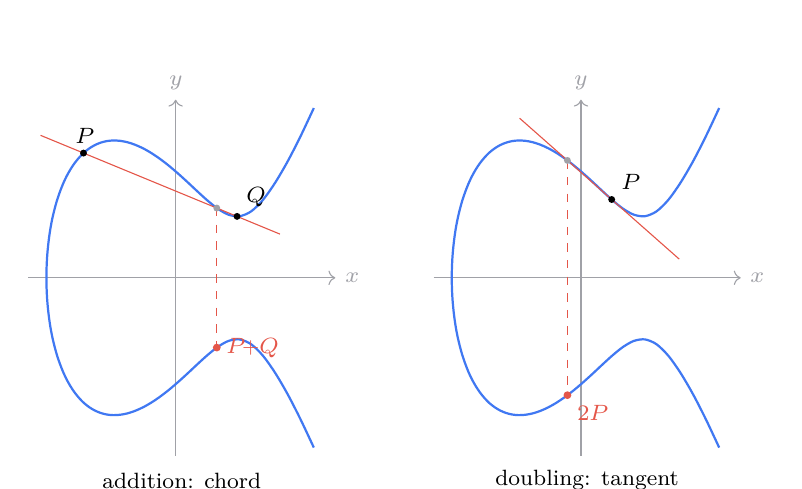
\begin{tikzpicture}[scale=0.78,font=\footnotesize]
\begin{scope}
  \draw[->,gray] (-2.4,0)--(2.6,0) node[right]{$x$}; \draw[->,gray] (0,-2.9)--(0,2.9) node[above]{$y$};
  \draw[acc,thick] plot[smooth] coordinates {(2.250,-2.764) (2.035,-2.307) (1.826,-1.899) (1.621,-1.549) (1.423,-1.270) (1.230,-1.082) (1.042,-1.003) (0.860,-1.028) (0.683,-1.127) (0.511,-1.265) (0.345,-1.416) (0.185,-1.566) (0.030,-1.706) (-0.120,-1.833) (-0.264,-1.943) (-0.403,-2.036) (-0.536,-2.111) (-0.664,-2.168) (-0.787,-2.208) (-0.904,-2.230) (-1.015,-2.236) (-1.121,-2.226) (-1.222,-2.200) (-1.317,-2.160) (-1.407,-2.106) (-1.492,-2.039) (-1.570,-1.959) (-1.644,-1.868) (-1.712,-1.766) (-1.775,-1.654) (-1.832,-1.533) (-1.883,-1.403) (-1.930,-1.266) (-1.970,-1.123) (-2.006,-0.973) (-2.036,-0.819) (-2.060,-0.660) (-2.079,-0.498) (-2.093,-0.333) (-2.101,-0.167) (-2.104,-0.000) (-2.101,0.167) (-2.093,0.333) (-2.079,0.498) (-2.060,0.660) (-2.036,0.819) (-2.006,0.973) (-1.970,1.123) (-1.930,1.266) (-1.883,1.403) (-1.832,1.533) (-1.775,1.654) (-1.712,1.766) (-1.644,1.868) (-1.570,1.959) (-1.492,2.039) (-1.407,2.106) (-1.317,2.160) (-1.222,2.200) (-1.121,2.226) (-1.015,2.236) (-0.904,2.230) (-0.787,2.208) (-0.664,2.168) (-0.536,2.111) (-0.403,2.036) (-0.264,1.943) (-0.120,1.833) (0.030,1.706) (0.185,1.566) (0.345,1.416) (0.511,1.265) (0.683,1.127) (0.860,1.028) (1.042,1.003) (1.230,1.082) (1.423,1.270) (1.621,1.549) (1.826,1.899) (2.035,2.307) (2.250,2.764)};
  \draw[warn] (-2.2,2.320)--(1.7,0.711);
  \draw[warn,dashed] (0.670,1.136)--(0.670,-1.136);
  \fill (-1.5,2.031) circle (1.6pt) node[above]{$P$};
  \fill (1.0,1.0) circle (1.6pt) node[above right]{$Q$};
  \fill[gray] (0.670,1.136) circle (1.6pt);
  \fill[warn] (0.670,-1.136) circle (1.8pt) node[right]{$P{+}Q$};
  \node at (0.1,-3.3) {addition: chord};
\end{scope}
\begin{scope}[xshift=6.6cm]
  \draw[->,gray] (-2.4,0)--(2.6,0) node[right]{$x$}; \draw[->,gray] (0,-2.9)--(0,2.9) node[above]{$y$};
  \draw[acc,thick] plot[smooth] coordinates {(2.250,-2.764) (2.035,-2.307) (1.826,-1.899) (1.621,-1.549) (1.423,-1.270) (1.230,-1.082) (1.042,-1.003) (0.860,-1.028) (0.683,-1.127) (0.511,-1.265) (0.345,-1.416) (0.185,-1.566) (0.030,-1.706) (-0.120,-1.833) (-0.264,-1.943) (-0.403,-2.036) (-0.536,-2.111) (-0.664,-2.168) (-0.787,-2.208) (-0.904,-2.230) (-1.015,-2.236) (-1.121,-2.226) (-1.222,-2.200) (-1.317,-2.160) (-1.407,-2.106) (-1.492,-2.039) (-1.570,-1.959) (-1.644,-1.868) (-1.712,-1.766) (-1.775,-1.654) (-1.832,-1.533) (-1.883,-1.403) (-1.930,-1.266) (-1.970,-1.123) (-2.006,-0.973) (-2.036,-0.819) (-2.060,-0.660) (-2.079,-0.498) (-2.093,-0.333) (-2.101,-0.167) (-2.104,-0.000) (-2.101,0.167) (-2.093,0.333) (-2.079,0.498) (-2.060,0.660) (-2.036,0.819) (-2.006,0.973) (-1.970,1.123) (-1.930,1.266) (-1.883,1.403) (-1.832,1.533) (-1.775,1.654) (-1.712,1.766) (-1.644,1.868) (-1.570,1.959) (-1.492,2.039) (-1.407,2.106) (-1.317,2.160) (-1.222,2.200) (-1.121,2.226) (-1.015,2.236) (-0.904,2.230) (-0.787,2.208) (-0.664,2.168) (-0.536,2.111) (-0.403,2.036) (-0.264,1.943) (-0.120,1.833) (0.030,1.706) (0.185,1.566) (0.345,1.416) (0.511,1.265) (0.683,1.127) (0.860,1.028) (1.042,1.003) (1.230,1.082) (1.423,1.270) (1.621,1.549) (1.826,1.899) (2.035,2.307) (2.250,2.764)};
  \draw[warn] (-1.0,2.599)--(1.6,0.304);
  \draw[warn,dashed] (-0.221,1.911)--(-0.221,-1.911);
  \fill (0.5,1.275) circle (1.6pt) node[above right]{$P$};
  \fill[gray] (-0.221,1.911) circle (1.6pt);
  \fill[warn] (-0.221,-1.911) circle (1.8pt) node[below right]{$2P$};
  \node at (0.1,-3.3) {doubling: tangent};
\end{scope}
\end{tikzpicture}
\end{center}

\textbf{Deriving the formulas.} Let the line through $P = (x_1, y_1)$ have slope $s$: $y = s(x - x_1) + y_1$. Substituting into $y^2 = x^3 + ax + b$ gives a cubic in $x$ whose expanded form starts $x^3 - s^2 x^2 + \dots = 0$. Its three roots are the $x$-coordinates of the three intersection points, and the sum of the roots of a monic cubic is minus the $x^2$ coefficient, so $x_1 + x_2 + x_3 = s^2$, giving $x_3 = s^2 - x_1 - x_2$. The third point is $(x_3,\ s(x_3 - x_1) + y_1)$; reflecting it gives $y_3 = s(x_1 - x_3) - y_1$. For addition, $s$ is the chord slope $(y_2 - y_1)/(x_2 - x_1)$. For doubling, $s$ is the tangent slope: differentiating $y^2 = x^3 + ax + b$ implicitly gives $2y\,y' = 3x^2 + a$, so $s = (3x_1^2 + a)/(2y_1)$, and $x_2 = x_1$. The constant $b$ vanishes on differentiation, which is why the doubling slope contains $a$ and never $b$.

\subsection{Elliptic curves over GF$(p)$ \new}
\likely{Find all the points on $E_{13}(1, 1)$ / $E_{11}(1, 6)$'' and find the inverse of a point'' (3--4 marks).}

Cryptography cannot use real numbers (rounding errors, unbounded size), so the same equation is taken modulo a prime $p > 3$. The curve $E_p(a, b)$ is the set of all pairs $(x, y) \in \mathbb{Z}_p \times \mathbb{Z}_p$ with
\[
y^2 \equiv x^3 + ax + b \pmod p, \qquad a, b \in \mathbb{Z}_p,\quad 4a^3 + 27b^2 \not\equiv 0 \pmod p,
\]
together with the point at infinity $O$. The curve'' is now a finite scatter of points, but the addition formulas derived above still define a group, with every division done as multiplication by an inverse modulo $p$.

\textbf{Finding the points.} For each $x = 0, 1, \dots, p-1$, compute $w = (x^3 + ax + b) \bmod p$, which must equal $y^2$. If $w = 0$ there is one point $(x, 0)$. If $w$ is a nonzero \textbf{quadratic residue} (a perfect square mod $p$), there are two points $(x, \sqrt w)$ and $(x, p - \sqrt w)$. If $w$ is not a square, no point has that $x$. Make the table of squares $y^2 \bmod p$ first; since $(p - y)^2 \equiv y^2$, only $y = 0, \dots, (p-1)/2$ are needed.

\textbf{Negatives.} The inverse of $P = (x, y)$ is $-P = (x, -y) = (x, p - y)$: the same $x$, only $y$ flipped (the reflection in the $x$-axis). A point with $y = 0$ is its own inverse. Points therefore come in vertical pairs $(x, y), (x, p - y)$.

\textbf{Hasse's theorem.} The number of points $\#E$ (including $O$) satisfies $p + 1 - 2\sqrt p \le \#E \le p + 1 + 2\sqrt p$: about half the $x$ values give a square and those give two points each, so \#E is close to $p + 1$. It is a quick check on a point count.

\begin{worked}[: Forouzan/slide, all points of $E_{13}(1, 1)$]
\textbf{Q.} Find all points on $E_{13}(1, 1)$: $y^2 = x^3 + x + 1 \pmod{13}$. List the inverse pairs.

\textbf{Valid curve}: $4 + 27 = 31 \equiv 5 \not\equiv 0 \pmod{13}$. \textbf{Squares mod 13}: $y = 0..6$ give $y^2 = 0, 1, 4, 9, 3, 12, 10$, so the nonzero squares are $\{1, 3, 4, 9, 10, 12\}$ with roots $1 \to \pm1$, $3 \to \pm4$, $4 \to \pm2$, $9 \to \pm3$, $10 \to \pm6$, $12 \to \pm5$.
\begin{center}\small
\begin{tabular}{@{}rrrcl@{}}
\toprule
$x$ & $x^3 + x + 1$ & $w$ & square? & points\\
\midrule
0 & 1 & 1 & yes & (0, 1), (0, 12)\\
1 & 3 & 3 & yes & (1, 4), (1, 9)\\
2 & 11 & 11 & no & --\\
3 & 31 & 5 & no & --\\
4 & 69 & 4 & yes & (4, 2), (4, 11)\\
5 & 131 & 1 & yes & (5, 1), (5, 12)\\
6 & 223 & 2 & no & --\\
7 & 351 & 0 & $y = 0$ & (7, 0)\\
8 & 521 & 1 & yes & (8, 1), (8, 12)\\
9 & 739 & 11 & no & --\\
10 & 1011 & 10 & yes & (10, 6), (10, 7)\\
11 & 1343 & 4 & yes & (11, 2), (11, 11)\\
12 & 1741 & 12 & yes & (12, 5), (12, 8)\\
\bottomrule
\end{tabular}
\end{center}
\textbf{17 points + $O$ = 18.} Each row's two points are inverses (e.g.\ $4 + 9 = 13$, so $(1, 9) = -(1, 4)$); $(7, 0)$ is its own inverse. $x = 2, 3, 6, 9$ give non-squares. Hasse: $14 \pm 2\sqrt{13} = [6.8,\ 21.2]$ contains 18 \checkmark.
\end{worked}

\begin{worked}[: new, all points of $E_{11}(1, 6)$]
\textbf{Q.} Find all points on $y^2 = x^3 + x + 6 \pmod{11}$ and verify Hasse's bound.

\textbf{Valid}: $4 + 27 \cdot 36 = 976 = 88 \cdot 11 + 8 \not\equiv 0$. \textbf{Squares mod 11}: $y = 0..5$ give $0, 1, 4, 9, 5, 3$; nonzero squares $\{1, 3, 4, 5, 9\}$ with roots $1 \to \pm1$, $3 \to \pm5$, $4 \to \pm2$, $5 \to \pm4$, $9 \to \pm3$.
\begin{center}\small
\begin{tabular}{@{}rrrcl@{\qquad}rrrcl@{}}
\toprule
$x$ & $x^3{+}x{+}6$ & $w$ & sq? & points & $x$ & $x^3{+}x{+}6$ & $w$ & sq? & points\\
\midrule
0 & 6 & 6 & no & -- & 6 & 228 & 8 & no & --\\
1 & 8 & 8 & no & -- & 7 & 356 & 4 & yes & (7, 2), (7, 9)\\
2 & 16 & 5 & yes & (2, 4), (2, 7) & 8 & 526 & 9 & yes & (8, 3), (8, 8)\\
3 & 36 & 3 & yes & (3, 5), (3, 6) & 9 & 744 & 7 & no & --\\
4 & 74 & 8 & no & -- & 10 & 1016 & 4 & yes & (10, 2), (10, 9)\\
5 & 136 & 4 & yes & (5, 2), (5, 9) & & & & & \\
\bottomrule
\end{tabular}
\end{center}
\textbf{12 points + $O$ = 13.} Hasse: $12 \pm 2\sqrt{11} = [5.4,\ 18.6]$ contains 13 \checkmark. Since 13 is prime, every point except $O$ generates the whole group (Lagrange).
\end{worked}

\subsection{Point addition and doubling over GF$(p)$ \new}
\likely{``Add $P$ and $Q$ / find $2P$ on $E_p(a, b)$'' (2--3 marks), always with modular inverses.}

\begin{mustknow}[: EC group law over GF$(p)$]
For $P = (x_1, y_1)$, $Q = (x_2, y_2)$, \;$R = P + Q = (x_3, y_3)$ with
\[
x_3 = s^2 - x_1 - x_2 \bmod p, \qquad y_3 = s(x_1 - x_3) - y_1 \bmod p,
\]
\[
s = \frac{y_2 - y_1}{x_2 - x_1} \bmod p \ \ (P \ne Q,\ \text{addition}), \qquad s = \frac{3x_1^2 + a}{2y_1} \bmod p \ \ (P = Q,\ \text{doubling}).
\]
Division means multiplying by the inverse mod $p$. Special cases: $P + O = P$; if $x_1 = x_2$ and $y_2 = -y_1$ then $P + Q = O$; doubling a point with $y_1 = 0$ gives $O$.
\end{mustknow}

\begin{worked}[: one addition and two doublings]
\textbf{Q1 (Forouzan style).} On $E_{13}(1, 1)$, add $P = (4, 2)$ and $Q = (10, 6)$.\\
$s = (6 - 2)(10 - 4)^{-1} = 4 \cdot 6^{-1} = 4 \cdot 11 = 44 \equiv 5$ \;($6 \cdot 11 = 66 = 5 \cdot 13 + 1$).\\
$x_3 = 25 - 4 - 10 = 11$; \;$y_3 = 5(4 - 11) - 2 = -37 \equiv -37 + 39 = 2$. \;$\mathbf{P + Q = (11, 2)}$, which is in the point list \checkmark.

\textbf{Q2.} On $E_{13}(1, 1)$, find $2P$ for $P = (1, 4)$.\\
$s = (3 \cdot 1^2 + 1)(2 \cdot 4)^{-1} = 4 \cdot 8^{-1} = 4 \cdot 5 = 20 \equiv 7$ \;($8 \cdot 5 = 40 = 3 \cdot 13 + 1$).\\
$x_3 = 49 - 1 - 1 = 47 \equiv 8$; \;$y_3 = 7(1 - 8) - 4 = -53 \equiv -53 + 65 = 12$. \;$\mathbf{2P = (8, 12)}$ \checkmark.

\textbf{Q3 (slide).} On $E_{17}(2, 2)$: $y^2 = x^3 + 2x + 2$, find $2P$ for $P = (5, 1)$.\\
$s = (3 \cdot 5^2 + 2)(2 \cdot 1)^{-1} = 77 \cdot 2^{-1} \equiv 9 \cdot 9 = 81 \equiv 13$ \;($77 = 4 \cdot 17 + 9$, $2^{-1} = 9$).\\
$x_3 = 169 - 5 - 5 = 159 = 9 \cdot 17 + 6 \equiv 6$; \;$y_3 = 13(5 - 6) - 1 = -14 \equiv 3$. \;$\mathbf{2P = (6, 3)}$.\\
Check: $3^2 = 9$ and $6^3 + 2 \cdot 6 + 2 = 230 = 13 \cdot 17 + 9$ \checkmark. (This curve has 19 points and $(5, 1)$ generates all of them.)
\end{worked}

\begin{trap}[: point arithmetic slips]
The doubling slope uses $a$ (from $3x^2 + a$), never $b$. Compute $s$ as an integer mod $p$ with a modular inverse, never as a fraction or decimal. $-P = (x, p - y)$ flips only $y$. Use the addition formula only for $P \ne Q$ (it would divide by $x_2 - x_1 = 0$). Reduce negative results by adding multiples of $p$, and check the answer lies on the curve.
\end{trap}

\subsection{Scalar multiplication and the ECDLP \new}
\likely{``Compute $kP$ for small $k$ and ``state the ECDLP / Hasse's theorem.}
Multiplying a point by an integer $k$ means adding it to itself: $kP = P + P + \dots + P$ ($k$ times). It is computed by \textbf{double-and-add}, the analogue of square-and-multiply: scan the bits of $k$, double at every bit and add $P$ at every 1-bit, so $kP$ costs about $\log_2 k$ doublings. The slides' two examples on $E_{13}(1, 1)$, recomputed:
\begin{itemize}[leftmargin=1.4em]
  \item $4 \cdot (1, 4) = 2 \cdot (2 \cdot (1, 4)) = 2 \cdot (8, 12)$: $s = (3 \cdot 64 + 1) \cdot 24^{-1} \equiv 11 \cdot 11^{-1} = 1$, $x_3 = 1 - 16 \equiv 11$, $y_3 = 1 \cdot (8 - 11) - 12 = -15 \equiv 11$, so $4 \cdot (1, 4) = \mathbf{(11, 11)}$ \checkmark.
  \item $3 \cdot (8, 1) = 2 \cdot (8, 1) + (8, 1)$: doubling gives $s = 193 \cdot 2^{-1} \equiv 11 \cdot 7 \equiv 12$, $(11, 2)$; then $(11, 2) + (8, 1)$: $s = (-1)(-3)^{-1} \equiv 12 \cdot 10^{-1} = 12 \cdot 4 \equiv 9$, $x_3 = 81 - 19 \equiv 10$, $y_3 = 9(11 - 10) - 2 = 7$, so $3 \cdot (8, 1) = \mathbf{(10, 7)}$ \checkmark.
\end{itemize}
$(1, 4)$ has order 18, so it generates all of $E_{13}(1, 1)$; its multiples (useful for checking the examples below) are:
\begin{center}\small
\begin{tabular}{@{}c|ccccccccc@{}}
\toprule
$k$ & 1 & 2 & 3 & 4 & 5 & 6 & 7 & 8 & 9\\
$k(1,4)$ & (1,4) & (8,12) & (0,12) & (11,11) & (5,1) & (10,6) & (12,8) & (4,2) & (7,0)\\
\midrule
$k$ & 17 & 16 & 15 & 14 & 13 & 12 & 11 & 10 & 18\\
$k(1,4)$ & (1,9) & (8,1) & (0,1) & (11,2) & (5,12) & (10,7) & (12,5) & (4,11) & $O$\\
\bottomrule
\end{tabular}
\end{center}
The second row is the negative of the first ($(18 - k)P = -kP$), and $9P = (7, 0)$ has $y = 0$, so $18P = 2 \cdot 9P = O$.

\textbf{Elliptic curve discrete logarithm problem (ECDLP).} Given a point $P$ (ideally a generator) and $T = dP$, find $d$ with $1 \le d \le \#E$. Computing $T$ from $d$ takes about $\log_2 d$ doublings, but no shortcut is known for the reverse: on a well-chosen curve the best attack is a generic one such as \textbf{Pollard's rho}, which needs about $\sqrt{\#E}$ steps. On the toy curve the table answers it at once ($T = (4, 2) \Rightarrow d = 8$); for a 160-bit curve, $\sqrt{\#E} \approx 2^{80}$ steps is infeasible.

\subsection{ECC simulating ElGamal \new}
\likely{``Explain ECC encryption/decryption; verify the given example'' (the slide's $E_{67}(2, 3)$ example).}

ElGamal works in any group where the discrete log is hard, so it carries over by a dictionary: multiplication mod $p$ becomes point addition, exponentiation becomes scalar multiplication, and the inverse becomes the negative point. The plaintext must be encoded as a point $P$ on the curve.

\begin{mustknow}[: EC ElGamal]
\textbf{Keys (Bob)}: choose $E_p(a, b)$, a point $e_1$ on it, and an integer $d$; compute $e_2 = d \times e_1$. Public $(E_p(a, b), e_1, e_2)$, private $d$.\\
\textbf{Encrypt (Alice)}: fresh random $r$; \;$C_1 = r \times e_1$, \;$C_2 = P + r \times e_2$.\\
\textbf{Decrypt (Bob)}: $P = C_2 - (d \times C_1)$, where subtracting means adding the negative point.\\
Proof: $C_2 - d C_1 = P + r(d e_1) - d(r e_1) = P + (rd) e_1 - (dr) e_1 = P + O = P$.
\end{mustknow}

\begin{worked}[: the slide example on $E_{67}(2, 3)$, every step]
\textbf{Q.} Bob selects $E_{67}(2, 3)$, $e_1 = (2, 22)$, $d = 4$. Alice sends $P = (24, 26)$ with $r = 2$. Find $e_2$, $C_1$, $C_2$, and verify decryption.

\begin{center}\small
\begin{tabular}{@{}lllll@{}}
\toprule
Step & Slope $s$ (mod 67) & $x_3$ & $y_3$ & Result\\
\midrule
$2e_1 = 2(2, 22)$ & $14 \cdot 44^{-1} = 14 \cdot 32 \equiv 46$ & $2112 \equiv 35$ & $-1540 \equiv 1$ & $(35, 1)$\\
$4e_1 = 2(35, 1)$ & $3677 \cdot 2^{-1} \equiv 59 \cdot 34 \equiv 63$ & $3899 \equiv 13$ & $1385 \equiv 45$ & $(13, 45)$\\
$2e_2 = 2(13, 45)$ & $509 \cdot 90^{-1} \equiv 40 \cdot 35 \equiv 60$ & $3574 \equiv 23$ & $-645 \equiv 25$ & $(23, 25)$\\
$P + 2e_2$ & $(-1)(-1)^{-1} = 1$ & $-46 \equiv 21$ & $-23 \equiv 44$ & $(21, 44)$\\
$C_2 + (23, 42)$ & $(-2) \cdot 2^{-1} \equiv 66$ & $4312 \equiv 24$ & $-242 \equiv 26$ & $(24, 26)$\\
\bottomrule
\end{tabular}
\end{center}
\textbf{Keys}: $e_2 = 4 e_1 = (13, 45)$. \textbf{Encrypt}: $C_1 = 2 e_1 = (35, 1)$, $r e_2 = (23, 25)$, $C_2 = (24, 26) + (23, 25) = (21, 44)$.\\
\textbf{Decrypt}: $d \times C_1 = 4 \cdot (35, 1) = 8 e_1 = 2 e_2 = (23, 25)$ (two doublings, rows 2--3). Its negative is $(23, 67 - 25) = (23, 42)$, and $(21, 44) + (23, 42) = \mathbf{(24, 26)} = P$ \checkmark.\\
Inverses used: $44 \cdot 32 = 1408 = 21 \cdot 67 + 1$; $2 \cdot 34 = 68$; $23 \cdot 35 = 805 = 12 \cdot 67 + 1$ ($90 \equiv 23$).
\end{worked}

\begin{worked}[: new exam-style example on $E_{13}(1, 1)$]
\textbf{Q.} Bob uses $E_{13}(1, 1)$ with $e_1 = (1, 4)$ and private key $d = 3$. Alice encrypts the point $P = (4, 2)$ with $r = 2$. Find Bob's public key, the ciphertext, and verify decryption.

\begin{center}\small
\begin{tabular}{@{}lllll@{}}
\toprule
Step & Slope $s$ (mod 13) & $x_3$ & $y_3$ & Result\\
\midrule
$2e_1 = 2(1, 4)$ & $4 \cdot 8^{-1} = 4 \cdot 5 \equiv 7$ & $47 \equiv 8$ & $-53 \equiv 12$ & $(8, 12)$\\
$e_2 = (8, 12) + (1, 4)$ & $(-8)(-7)^{-1} = 5 \cdot 6^{-1} = 5 \cdot 11 \equiv 3$ & $0$ & $12$ & $(0, 12)$\\
$2e_2 = 2(0, 12)$ & $1 \cdot 24^{-1} = 11^{-1} = 6$ & $36 \equiv 10$ & $-72 \equiv 6$ & $(10, 6)$\\
$C_2 = (4, 2) + (10, 6)$ & $4 \cdot 6^{-1} \equiv 5$ & $11$ & $-37 \equiv 2$ & $(11, 2)$\\
$2C_1 = 2(8, 12)$ & $193 \cdot 24^{-1} \equiv 11 \cdot 6 \equiv 1$ & $-15 \equiv 11$ & $-15 \equiv 11$ & $(11, 11)$\\
$3C_1 = (11, 11) + (8, 12)$ & $1 \cdot (-3)^{-1} = 10^{-1} = 4$ & $-3 \equiv 10$ & $-7 \equiv 6$ & $(10, 6)$\\
$C_2 + (10, 7)$ & $5 \cdot (-1)^{-1} = 5 \cdot 12 \equiv 8$ & $43 \equiv 4$ & $54 \equiv 2$ & $(4, 2)$\\
\bottomrule
\end{tabular}
\end{center}
\textbf{Public key} $(E_{13}(1, 1), (1, 4), (0, 12))$. \textbf{Ciphertext} $C_1 = 2 e_1 = \mathbf{(8, 12)}$, $C_2 = \mathbf{(11, 2)}$.\\
\textbf{Decrypt}: $d \times C_1 = 3 \cdot (8, 12) = (10, 6)$, the same point as $r \times e_2$; negative $(10, 7)$; $(11, 2) + (10, 7) = \mathbf{(4, 2)}$ \checkmark. In multiples of $e_1$ (table above): $e_2 = 3e_1$, $C_1 = 2e_1$, $P = 8e_1$, $C_2 = (8 + 6)e_1 = 14 e_1$, and $14 - 6 = 8$ \checkmark.
\end{worked}

\subsection{Security of ECC and key size \new}
\likely{``Why does ECC need smaller keys than RSA for the same security? (2 marks).}
To decrypt, Eve needs $r$ (then $P = C_2 - r \times e_2$) or $d$ (then $P = C_2 - d \times C_1$). Finding $r$ from $C_1 = r \times e_1$, or $d$ from $e_2 = d \times e_1$, is the ECDLP, which for large $p$ (or large $n$ in GF$(2^n)$) is infeasible by Pollard's rho. As in ElGamal, $r$ must be fresh for every message.

\textbf{Why ECC keys are smaller.} For factoring and for the discrete log in $\mathbb{Z}_p^*$ there are \textbf{sub-exponential} algorithms (the number field sieve, index calculus) that exploit the arithmetic structure of integers, so RSA and ElGamal need 1024-bit and larger moduli to stay ahead. On a well-chosen elliptic curve no such structure is known, and only generic attacks costing about $\sqrt{\#E}$ work, i.e.\ $2^{k/2}$ for a $k$-bit curve. A 160-bit curve therefore costs about $2^{80}$ steps, the same effort as factoring a 1024-bit RSA modulus: \imp{ECC over GF$(2^n)$ or GF$(p)$ with a 160-bit modulus gives the same security as RSA with a 1024-bit modulus} (and 256-bit ECC $\approx$ 3072-bit RSA). Smaller keys mean less computation, bandwidth and storage, which suits smart cards and mobile devices.


\begin{fixbox}
\begin{itemize}[leftmargin=1.2em,itemsep=0pt]
  \item ElGamal block diagram: the encryption box labels both lines $C_1$; the second line, $(e_2^r \cdot P) \bmod p$, is $\boldsymbol{C_2}$.
  \item $E_{67}(2, 3)$ example, step 8: ``He uses $2 \times C_1$'' should read $d \times C_1 = \boldsymbol{4} \times C_1 = (23, 25)$. With $C_1 = 2e_1$, $2 \times C_1 = 4e_1 = e_2 = (13, 45)$, not $(23, 25)$ (recomputed). The same misprint is in Forouzan.
  \item ElGamal security slide: 1024 bits is about \textbf{309} decimal digits (as on the RSA slide), not 300.
\end{itemize}
\end{fixbox}


\part{Integrity, Authentication and Key Management}
% College Lecture 14: message integrity, birthday problems, hash attacks, iterated hashes, SHA-512, Whirlpool.
% Sources: slides L14 (58 slides), Forouzan ch. 11 + 12. Every number recomputed by script (scratchpad/hash/verify*.py).
\section{Message Integrity and Hash Functions}\label{sec:integrity}
\usetikzlibrary{decorations.pathreplacing}

\subsection{Integrity versus secrecy; message and digest \new}
\likely{``Why is a hash, not encryption, used for integrity?'' and ``how is integrity checked with a digest?'' (2--3 marks).}

Every scheme so far gave \emph{secrecy}: Eve cannot read the message. Many documents need the opposite guarantee. Alice's will, for example, need not be encrypted, because after her death anyone may read it; what must be preserved is its \emph{integrity}, meaning that nobody can change its contents without the change being noticed. On paper this is achieved by putting Alice's fingerprint at the bottom of the document: Eve can read the will, but she cannot alter it or write a false one, because she cannot forge the fingerprint.

The electronic equivalent of the document--fingerprint pair is the \textbf{message--digest pair}. The message is passed through a \textbf{cryptographic hash function} $h$, which maps a message of any length to a short fixed-length string $h(M)$, called the \textbf{message digest}. The digest is a compressed image of the message that plays the role of the fingerprint. To check integrity later, the receiver runs the same hash function on the message he now holds and compares the new digest with the stored one: \imp{if the two digests are equal, the message has not been changed; if they differ, the message was changed and is discarded.}

\textbf{Why a hash and not encryption.} Encryption hides the message but does not stop Eve from altering the ciphertext; flipping a bit of a one-time-pad or stream-cipher ciphertext flips the same bit of the plaintext, and Bob has no way to tell a changed plaintext from a genuine one. A hash works the other way round: it hides nothing (the message can be public), but since any change to the message produces a different digest, any change is detected. The two services are therefore independent, and a message can need one, the other, or both.

\textbf{The digest itself must be safe.} The check only works if the stored or received digest is genuine. If Eve can replace both $M$ and $h(M)$, she simply sends $M'$ with $h(M')$ and the comparison passes. Hence the digest is kept in a safe place or sent over an authenticated channel; binding the digest to a secret key gives the MAC of the next lecture.

\subsection{The three security criteria \new}
\likely{``Define and differentiate preimage, second preimage and collision resistance'' (3--4 marks), possibly with a figure of what Eve is given and must find.}

A cryptographic hash function must make three kinds of forgery infeasible. They differ in how much Eve is given at the start, and therefore in how much freedom she has.

\textbf{Preimage resistance.} Given a hash function $h$ and a digest $y = h(M)$, it must be extremely difficult for Eve to find \emph{any} message $M'$ with $h(M') = y$. If $h$ were not preimage resistant, Eve could intercept just the digest $h(M)$, construct a message $M'$ that hashes to it, and send $M'$ to Bob as if it were $M$. In other words, the hash must be one-way.

\textbf{Second preimage resistance.} Given a specific message $M$ \emph{and} its digest $h(M)$, it must be extremely difficult to find another message $M' \ne M$ with $h(M') = h(M)$. This is the criterion that stops forgery of a particular message: if Alice sends $M$ and $h(M)$ to Bob, Eve cannot create a different message with the same digest and substitute it. Eve here has more information than in the preimage case (she also knows one valid preimage), but she still has to hit one fixed target value.

\textbf{Collision resistance.} It must be extremely difficult to find \emph{any} two messages $M \ne M'$ with $h(M) = h(M')$. Here Eve is given nothing and is free to choose both messages from scratch; such a pair is called a \textbf{collision}. This is the danger when Eve prepares two documents herself (say a fair contract and an unfair one with the same digest), gets Alice to approve the fair one, and later swaps in the other.

\begin{center}\small
\begin{tabularx}{\textwidth}{@{}l X X l@{}}
\toprule
Criterion & Eve is given & Eve must find & Attack it stops\\
\midrule
Preimage resistance & $h$ and a digest $y = h(M)$ & any $M'$ with $h(M') = y$ & preimage\\
Second preimage resistance & $h$, a message $M$ and $h(M)$ & $M' \ne M$ with $h(M') = h(M)$ & second preimage\\
Collision resistance & only $h$ & any pair $M \ne M'$ with $h(M) = h(M')$ & collision\\
\bottomrule
\end{tabularx}
\end{center}

\textbf{Collision resistance implies second preimage resistance.} Suppose Eve had a method that, given any $M$, produces a second preimage $M'$. She could then pick any $M$ she likes, run the method, and output the pair $(M, M')$, which is a collision. So a function that is \emph{not} second-preimage resistant cannot be collision resistant; equivalently, a collision-resistant function is automatically second-preimage resistant. The converse fails, because finding a collision is the easier task (Eve chooses both sides), and the birthday analysis below shows by how much: a collision costs about $2^{n/2}$ hash evaluations, a second preimage about $2^n$.

\textbf{Why a compressor or a checksum is not a cryptographic hash.} A lossless compression method such as ZIP or StuffIt also shrinks the message, but it is reversible: anyone can decompress the output and get the original, so it is not even a function to a fixed-length output, and it fails preimage resistance trivially. A checksum (adding up the bytes, a CRC) is fixed-length but linear and easy to invert: given a target checksum, Eve can compute what to change in any message to reach it, so it is neither preimage nor second-preimage resistant. Checksums detect accidental errors, not deliberate ones.

\begin{mustknow}[: the three criteria]
\textbf{Preimage}: given $y$, find any $M'$ with $h(M') = y$. \quad \textbf{Second preimage}: given $M$, find $M' \ne M$ with $h(M') = h(M)$. \quad \textbf{Collision}: find any $M \ne M'$ with $h(M) = h(M')$.\\
Cost for an ideal $n$-bit hash: preimage and second preimage $\approx 2^n$, collision $\approx 2^{n/2}$. Collision resistance $\Rightarrow$ second preimage resistance.
\end{mustknow}

\subsection{The random oracle model \new}
\likely{``Explain the random oracle model; why can the oracle not use a formula?'' (2--3 marks).}

To analyse attacks we need a model of a perfect hash function, against which real designs are compared. The \textbf{random oracle model} (Bellare and Rogaway, 1993) describes such an ideal function as an oracle that keeps a table of the messages it has already hashed and obeys three rules:
\begin{enumerate}[nosep]
  \item When a \emph{new} message of any length is given, the oracle creates a fixed-length digest that is a truly random string of 0s and 1s, gives it out, and records the message and digest in its table.
  \item When a message is given for which a digest already exists, the oracle simply returns the digest in the table. This makes the function deterministic: the same message always gets the same digest.
  \item The digest for a new message must be chosen independently of all previous digests. This implies that the oracle cannot use a formula or an algorithm to calculate the digest.
\end{enumerate}

\textbf{Example (slides 20--23).} An oracle with 16-bit digests already holds three entries. It is asked to hash \ttx{AB1234CD8765BDAD}, which is not in its table, so it flips a fair coin 16 times and gets \ttx{HHTHHHTTHTHHTTTH}. Reading H as 1 and T as 0 gives \ttx{1101 1100 1011 0001} $=$ \ttx{DCB1}, which it returns and records. When it is then asked for \ttx{4523AB1352CDEF45126}, which is already in the table, it does not flip again but returns the stored digest \ttx{13AB}.
\begin{center}\small
\begin{tabular}{@{}ll@{}}
\toprule
Message & Digest\\
\midrule
\ttx{4523AB1352CDEF45126} & \ttx{13AB}\\
\ttx{723BAE38F2AB3457AC} & \ttx{02CA}\\
\ttx{AB1234CD8765BDAD} & \ttx{DCB1} (new)\\
\ttx{AB45CD1048765412AAAB6662BE} & \ttx{A38B}\\
\bottomrule
\end{tabular}
\end{center}

\textbf{Why a formula violates rule 3.} Suppose the oracle used $h(M) = M \bmod n$ and had already issued $h(M_1)$ and $h(M_2)$. For the new message $M_3 = M_1 + M_2$ anyone can predict the digest without asking, since
\[
h(M_3) = (M_1 + M_2) \bmod n = [\,h(M_1) + h(M_2)\,] \bmod n .
\]
The digest of $M_3$ is therefore not independent of the earlier digests, which breaks rule 3. Real hash functions are algorithms, so they can only approximate the oracle; the model tells us the best security an $n$-bit design can hope for.

\textbf{What the model gives an attacker.} With an $n$-bit digest there are $N = 2^n$ possible digests, and each new message receives one of them uniformly at random. Some values may be chosen several times and some never. Eve knows the algorithm and $n$, so every attack reduces to drawing random digests and waiting for a match, which is exactly a birthday problem.

\subsection{The four birthday problems \new}
\likely{Derive the probability formula for one problem and get $k$ for $P = 1/2$; or ``how many people for a shared birthday'' (23).}

All four problems use a random variable that is uniform over $N$ values ($0$ to $N - 1$; $N = 365$ for birthdays) and ask for the minimum number of samples $k$ that makes an event \emph{likely}, meaning probability $P \ge 1/2$. Every derivation uses the approximation $1 - x \approx e^{-x}$ for small $x$.

\textbf{Problem 1: a sample equals a predefined value.} What is the minimum number of students such that it is likely that at least one has a \emph{predefined} birthday (say 1 January)? A single sample misses the target with probability $1 - 1/N$, and the $k$ samples are independent, so all of them miss with probability $(1 - 1/N)^k \approx e^{-k/N}$. Hence
\[
P_1 \approx 1 - e^{-k/N}, \qquad k \approx \ln\frac{1}{1-P}\times N \;\xrightarrow{P = 1/2}\; k \approx \ln 2 \times N = 0.69N .
\]
For $N = 365$: $0.693 \times 365 = 252.99$, so $k = 253$.

\textbf{Problem 2: a sample equals one chosen from the set.} What is the minimum number such that it is likely that at least one student has the same birthday as a student \emph{selected by the professor}? The selected student is one of the $k$, so only the other $k - 1$ can match, and the problem is Problem 1 with $k - 1$ samples:
\[
P_2 \approx 1 - e^{-(k-1)/N}, \qquad k \approx \ln 2 \times N + 1 = 0.69N + 1 ;\qquad N = 365:\ k = 254 .
\]

\textbf{Problem 3: any two samples are equal (the birthday paradox).} What is the minimum number such that it is likely that \emph{at least two} students share a birthday? It is easier to count the complement, that all $k$ values are different. The first value is free, the second must avoid 1 value, the $i$-th must avoid $i - 1$ values, so
\[
\Pr[\text{all different}] = \prod_{i=1}^{k-1}\Bigl(1 - \frac{i}{N}\Bigr) \approx \prod_{i=1}^{k-1} e^{-i/N} = e^{-(1 + 2 + \dots + (k-1))/N} = e^{-k(k-1)/2N}.
\]
Therefore
\[
P_3 \approx 1 - e^{-k(k-1)/2N}, \qquad k \approx \Bigl\{2\ln\frac{1}{1-P}\Bigr\}^{1/2} N^{1/2} \;\xrightarrow{P = 1/2}\; k \approx \sqrt{2\ln 2}\,\sqrt N = 1.18\sqrt N ,
\]
using $k(k-1) \approx k^2$. For $N = 365$: $1.18 \times 19.1 = 22.5$, so $k = 23$ (exactly, 23 people give $P = 0.507$ and 22 give $0.476$). The answer is a ``paradox'' only because intuition compares each person with \emph{one} date, whereas $k$ people form $k(k-1)/2 = 253$ pairs, each a chance to match.

\textbf{Problem 4: a sample of one set equals a sample of another.} Two classes each have $k$ students. What is the minimum $k$ such that it is likely that some student of the first class shares a birthday with some student of the second? Treat the $k$ values of set 1 as (nearly) distinct. Each value of set 2 then misses all of them with probability $1 - k/N$, and the $k$ values of set 2 all miss with probability $(1 - k/N)^k \approx e^{-k^2/N}$. Hence
\[
P_4 \approx 1 - e^{-k^2/N}, \qquad k \approx \Bigl\{\ln\frac{1}{1-P}\Bigr\}^{1/2} N^{1/2} \;\xrightarrow{P = 1/2}\; k \approx \sqrt{\ln 2}\,\sqrt N = 0.83\sqrt N ;\qquad N = 365:\ k = 16 .
\]
(Exactly, $k = 16$ gives $P = 0.504$.)

\begin{center}\small
\begin{tabular}{@{}clllcl@{}}
\toprule
Problem & Probability $P$ & General $k$ & $k$ at $P = \tfrac12$ & $N = 365$ & Attack\\
\midrule
1 & $1 - e^{-k/N}$ & $\ln\frac{1}{1-P} \cdot N$ & $0.69N$ & 253 & preimage\\
2 & $1 - e^{-(k-1)/N}$ & $\ln\frac{1}{1-P} \cdot N + 1$ & $0.69N + 1$ & 254 & second preimage\\
3 & $1 - e^{-k(k-1)/2N}$ & $\{2\ln\frac{1}{1-P}\}^{1/2} N^{1/2}$ & $1.18\sqrt N$ & 23 & collision\\
4 & $1 - e^{-k^2/N}$ & $\{\ln\frac{1}{1-P}\}^{1/2} N^{1/2}$ & $0.83\sqrt N$ & 16 & alternate collision\\
\bottomrule
\end{tabular}
\end{center}
The constants are $0.69 = \ln 2$, $1.18 = \sqrt{2\ln 2}$ and $0.83 = \sqrt{\ln 2}$. The key comparison is that \textbf{$k$ grows like $N$ in Problems 1 and 2 but only like $\sqrt N$ in Problems 3 and 4}. Problems 1 and 2 model the preimage and second preimage attacks, Problems 3 and 4 the collision attacks, so a collision attack is far cheaper than a preimage attack on the same hash.

\begin{trap}[: rounding the constant]
With $0.69$ exactly, $0.69 \times 365 = 251.85$, which would suggest 252; the table value 253 comes from $\ln 2 = 0.6931$ ($0.6931 \times 365 = 252.99$). Use $0.693$ when the answer must be an exact head count. Also do not mix up Problems 1 and 3: ``someone has \emph{my} birthday'' needs 253 people, ``\emph{some two} share a birthday'' needs only 23.
\end{trap}

\begin{worked}[: birthday numbers for a 16-bit digest]
\textbf{Q.} A hash function produces 16-bit digests. Using the birthday results, how many random messages must Eve hash for a probability of at least $1/2$ of (a) matching a given digest, (b) finding any two messages with the same digest, (c) a match between two lists of $k$ messages each?

\textbf{A.} $N = 2^{16} = 65\,536$ and $\sqrt N = 2^8 = 256$.\\
(a) Problem 1: $k \approx 0.69 \times 65\,536 \approx 45\,220$ messages (order $2^{16}$).\\
(b) Problem 3: $k \approx 1.18 \times 256 \approx \mathbf{302}$ messages (order $2^8$).\\
(c) Problem 4: $k \approx 0.83 \times 256 \approx \mathbf{213}$ messages in each list.\\
\emph{Check}: (b) is about 150 times cheaper than (a), as $2^{16}/2^8 = 256$ predicts up to the constants.
\end{worked}

\subsection{Attacks on an $n$-bit digest \new}
\likely{``A hash uses a 64-bit digest; how many digests must Eve create to find a collision (or the original message) with $P > 0.5$, and how long does it take?'' (3--4 marks).}

Assume the hash behaves like a random oracle with $n$-bit digests, so its outputs are uniform over $N = 2^n$ values, and that Eve knows the algorithm and $n$. Each attack below is a loop that creates messages, hashes them, and compares digests; its success probability is the matching birthday problem.

\textbf{Preimage attack.} Eve has intercepted a digest $D = h(M)$ and wants any $M'$ with $h(M') = D$. She creates $k$ messages $M[1], \dots, M[k]$, computes $T = h(M[i])$ for each, and returns $M[i]$ as soon as $T = D$. The target $D$ is a predefined value, so this is Problem 1: $P = 1 - e^{-k/N}$, and success with $P \ge 1/2$ needs $k = 0.69 \times 2^n$ digests, which is of order $2^n$.

\textbf{Second preimage attack.} Eve has intercepted both $M$ and $D = h(M)$ and wants $M' \ne M$ with $h(M') = D$. She creates $k - 1$ further messages and compares each digest with $D$. The target is one of the $k$ samples (the given $M$), so this is Problem 2: $P = 1 - e^{-(k-1)/N}$ and $k = 0.69 \times 2^n + 1$, again of order $2^n$.

\textbf{Collision attack.} Eve wants any $M \ne M'$ with $h(M) = h(M')$. She creates $k$ messages, stores the digests $D[1], \dots, D[k]$, and compares each new digest with all earlier ones. Any two equal digests suffice, so this is Problem 3: $P = 1 - e^{-k(k-1)/2N}$ and $k = 1.18 \times 2^{n/2}$, of order only $2^{n/2}$. The square root comes from the number of pairs: $k$ digests give about $k^2/2$ pairs, and once $k^2/2$ is comparable to $2^n$ a coincidence is likely.

\textbf{Alternate collision attack.} A random collision is usually useless, because the two colliding messages are meaningless strings. A real forger needs a collision between a \emph{genuine} message $M$ (which Alice will approve) and a \emph{bogus} message $M'$ (which Eve will later substitute), both meaningful. Eve therefore makes $k$ variants of each without changing their meaning (an extra space after a word, a synonym, ``will not'' versus ``won't'', a redundant phrase): $M_1, \dots, M_k$ and $M'_1, \dots, M'_k$. She hashes both lists and looks for $h(M_i) = h(M'_j)$. A match must be \emph{across} the two lists, so this is Problem 4: $P = 1 - e^{-k^2/N}$ and $k = 0.83 \times 2^{n/2}$ variants of each, still of order $2^{n/2}$. Variants are cheap to produce: if a letter has $n/2$ independent places where one of two equivalent forms can be used, it has $2^{n/2}$ variants.

\begin{center}\small
\begin{tabular}{@{}llll@{}}
\toprule
Attack & Birthday problem & $k$ for $P = 1/2$ & Order\\
\midrule
Preimage & 1 & $0.69 \times 2^n$ & $2^n$\\
Second preimage & 2 & $0.69 \times 2^n + 1$ & $2^n$\\
Collision & 3 & $1.18 \times 2^{n/2}$ & $2^{n/2}$\\
Alternate collision & 4 & $0.83 \times 2^{n/2}$ & $2^{n/2}$\\
\bottomrule
\end{tabular}
\end{center}

\begin{worked}[: a 64-bit digest (slides 27 and 32)]
\textbf{Q.} A cryptographic hash function uses a 64-bit digest. (a) How many digests must Eve create to find the original message with probability more than $0.5$, and how long does it take at $2^{30}$ (about one billion) digests per second? (b) How many digests must she create to find two messages with the same digest with probability more than $0.5$, and how long does it take at $2^{20}$ (about one million) digests per second? Is a 64-bit digest secure?

\textbf{A.} $n = 64$, $N = 2^{64}$.\\
(a) Preimage attack (Problem 1): $k = 0.69 \times 2^{64} \approx 1.27 \times 10^{19}$ digests.\\
Time $= 0.69 \times 2^{64} / 2^{30} = 0.69 \times 2^{34}$ s $= 1.185 \times 10^{10}$ s $\div (3.156 \times 10^{7}$ s/year$) \approx \mathbf{376}$ \textbf{years}. Secure against the preimage attack.\\
(b) Collision attack (Problem 3): $k = 1.18 \times 2^{64/2} = 1.18 \times 2^{32} \approx 5.07 \times 10^{9}$ digests.\\
Time $= 1.18 \times 2^{32} / 2^{20} = 1.18 \times 2^{12}$ s $= 4833$ s $\approx \mathbf{1.34}$ \textbf{hours}. \textbf{Not} secure against the collision attack, even with a computer a thousand times slower.\\
\emph{Check}: the collision attack is cheaper by about $2^{32}$ in digests, exactly the gap between $2^n$ and $2^{n/2}$.
\end{worked}

\textbf{What digest length is needed.} Since the cheapest generic attack costs about $2^{n/2}$ hash evaluations, an $n$-bit hash offers only $n/2$ bits of security against collisions. To demand at least $2^{80}$ work, the digest must have $n/2 \ge 80$, i.e.\ $n \ge 160$ bits, which is why SHA-1 has 160 bits and the SHA-2 family 224--512 bits. \textbf{MD5's 128-bit digest} gives only $2^{64}$ collision security: $1.18 \times 2^{64} \approx 2.2 \times 10^{19}$ digests, about 640 years on one machine at $2^{30}$ per second, but well within reach of a large cluster. In addition, structural attacks (Wang et al., 2004) now find MD5 collisions in minutes on a PC, so MD5 must not be used where collisions matter.

\begin{worked}[: new exam-style numerical]
\textbf{Q.} A hash function produces 40-bit digests and Eve can compute $2^{20}$ digests per second. (a) How long does a preimage attack with success probability $1/2$ take? (b) How long does a collision attack take? (c) If Eve hashes $2^{20}$ messages, what is the probability that two of them collide?

\textbf{A.} $N = 2^{40}$.\\
(a) $k = 0.69 \times 2^{40}$; time $= 0.69 \times 2^{20}$ s $= 723\,517$ s $\approx \mathbf{8.4}$ \textbf{days}.\\
(b) $k = 1.18 \times 2^{20} \approx 1.24 \times 10^{6}$; time $= 1.18$ s, \textbf{about one second}.\\
(c) $P = 1 - e^{-k(k-1)/2N} \approx 1 - e^{-2^{40}/2^{41}} = 1 - e^{-0.5} = \mathbf{0.39}$.\\
\emph{Check}: (b) is (a) divided by roughly $2^{20}$, consistent with the orders $2^{40}$ and $2^{20}$.
\end{worked}

\begin{worked}[: how many variants for an alternate collision]
\textbf{Q.} Eve attacks a 64-bit hash with the alternate collision attack. How many variants of the genuine and the bogus letter does she need for success probability about $1/2$, and how many two-way choice points must each letter contain? What is her success probability with $2^{32}$ variants of each?

\textbf{A.} Problem 4: $k = 0.83 \times 2^{64/2} = 0.83 \times 2^{32} \approx 3.56 \times 10^{9}$ variants of each letter. With $m$ independent places where one of two equivalent forms can be chosen, a letter has $2^m$ variants, so $m = 32$ choice points per letter are enough ($2^{32} > 0.83 \times 2^{32}$).\\
With $k = 2^{32}$: $P = 1 - e^{-k^2/N} = 1 - e^{-2^{64}/2^{64}} = 1 - e^{-1} = \mathbf{0.63}$.
\end{worked}

\subsection{Iterated hash functions: the Merkle--Damg\aa rd scheme \new}
\likely{``Explain the Merkle--Damg\aa rd scheme with a diagram'' (3--4 marks).}

A hash function must accept messages of any length and still produce a fixed-length digest, and designing one function for arbitrary input lengths directly is hard. The standard solution is \textbf{iteration}: design a \textbf{compression function} $f$ with \emph{fixed-size} input, which compresses an $(n + m)$-bit input (an $n$-bit message block and an $m$-bit chaining value) to $m$ bits, and apply it as many times as the message requires. A hash built this way is an \textbf{iterated cryptographic hash function}, and the \textbf{Merkle--Damg\aa rd scheme} is the standard way of doing it.

\begin{center}
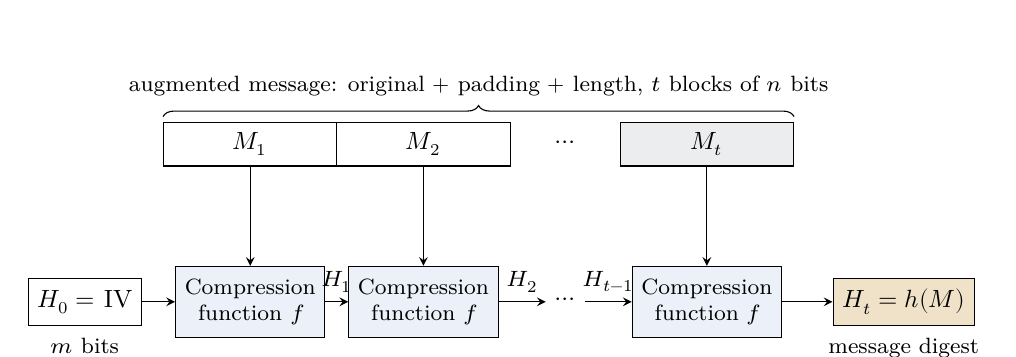
\begin{tikzpicture}[font=\small, >=stealth,
  fbox/.style={draw, fill=acc!8, minimum width=1.7cm, minimum height=0.9cm, align=center, font=\footnotesize},
  mbox/.style={draw, minimum width=2.2cm, minimum height=0.55cm}]
\node[mbox] (m1) at (0,2) {$M_1$};
\node[mbox] (m2) at (2.2,2) {$M_2$};
\node (dots) at (4.0,2) {$\cdots$};
\node[mbox, fill=gray!15] (mt) at (5.8,2) {$M_t$};
\draw[decorate,decoration={brace,amplitude=4pt}] ([yshift=2pt]m1.north west) -- node[above=4pt]{\footnotesize augmented message: original $+$ padding $+$ length, $t$ blocks of $n$ bits} ([yshift=2pt]mt.north east);
\node[draw, minimum width=1cm, minimum height=0.6cm] (h0) at (-2.1,0) {$H_0 = $ IV};
\node[fbox] (f1) at (0,0) {Compression\\function $f$};
\node[fbox] (f2) at (2.2,0) {Compression\\function $f$};
\node at (4.0,0) (d2) {$\cdots$};
\node[fbox] (ft) at (5.8,0) {Compression\\function $f$};
\node[draw, minimum width=1cm, minimum height=0.6cm, fill=gold!20] (ht) at (8.3,0) {$H_t = h(M)$};
\draw[->] (m1) -- (f1); \draw[->] (m2) -- (f2); \draw[->] (mt) -- (ft);
\draw[->] (h0) -- (f1); \draw[->] (f1) -- node[above]{\footnotesize $H_1$} (f2);
\draw[->] (f2) -- node[above]{\footnotesize $H_2$} (d2); \draw[->] (d2) -- node[above]{\footnotesize $H_{t-1}$} (ft);
\draw[->] (ft) -- (ht);
\node[below=1pt of h0, font=\footnotesize] {$m$ bits};
\node[below=1pt of ht, font=\footnotesize] {message digest};
\end{tikzpicture}
\end{center}

The scheme works in five steps.
\begin{enumerate}[nosep]
  \item The message length and padding are appended to the message to create an \textbf{augmented message} whose length is a multiple of $n$, the block size of the compression function.
  \item The augmented message is split into $t$ blocks $M_1, M_2, \dots, M_t$ of $n$ bits each.
  \item Before the iteration starts, the chaining value $H_0$ is set to a fixed public value called the \textbf{IV} (initial value).
  \item Iteration $i$ combines the previous digest with the next block: $H_i = f(H_{i-1}, M_i)$ for $i = 1, \dots, t$.
  \item The last chaining value $H_t$ is the hash of the original message, $h(M) = H_t$.
\end{enumerate}

\textbf{Why it is collision resistant if $f$ is.} Suppose two different messages $M \ne M'$ gave the same final digest $H_t = H'_t$. Then the last compression steps $f(H_{t-1}, M_t)$ and $f(H'_{t-1}, M'_t)$ have equal outputs. If their inputs differ, that is a collision of $f$. If their inputs are equal, then $H_{t-1} = H'_{t-1}$ and the same argument applies one step earlier, and so on backwards. Since $M \ne M'$, the inputs must differ at some step, so a collision of $h$ always yields a collision of $f$. The length field is essential to this argument: it puts the message length in the last block, so two messages of different lengths already differ in their final inputs and cannot be lined up to share a suffix. As a result, the designer only has to make one fixed-size function collision resistant.

\subsection{Compression functions: from scratch or from a block cipher \new}
\likely{``Differentiate Rabin, Davies--Meyer and Miyaguchi--Preneel; why is Rabin weak?'' (3 marks).}

There are two ways to obtain the compression function $f$. In the first, $f$ is \textbf{designed from scratch} specifically for hashing; in the second, an existing \textbf{symmetric-key block cipher} is used as $f$, so that the confidence gained in the cipher carries over.

\textbf{Made from scratch: the MD and SHA families.} The \textbf{Message Digest} family by Rivest has several versions (MD2, MD4, MD5). MD5 is a strengthened MD4 that divides the message into 512-bit blocks and creates a 128-bit digest; this digest turned out to be too short to resist collision attacks. The \textbf{Secure Hash Algorithm} family, the NIST standard also called the Secure Hash Standard (SHS), started with SHA (later SHA-1) and added SHA-224, SHA-256, SHA-384 and SHA-512 (together called SHA-2). All of them are Merkle--Damg\aa rd constructions.
\begin{center}\small
\begin{tabular}{@{}lcccccc@{}}
\toprule
Characteristic & MD5 & SHA-1 & SHA-224 & SHA-256 & SHA-384 & SHA-512\\
\midrule
Maximum message size (bits) & any$^{*}$ & $2^{64} - 1$ & $2^{64} - 1$ & $2^{64} - 1$ & $2^{128} - 1$ & $2^{128} - 1$\\
Block size (bits) & 512 & 512 & 512 & 512 & 1024 & 1024\\
Digest size (bits) & 128 & 160 & 224 & 256 & 384 & 512\\
Number of rounds / steps & 64 & 80 & 64 & 64 & 80 & 80\\
Word size (bits) & 32 & 32 & 32 & 32 & 64 & 64\\
\bottomrule
\end{tabular}
\end{center}
The SHA columns are the slide's table (slide 41); the MD5 column is added for comparison ($^{*}$MD5 records the length modulo $2^{64}$, so it accepts any length). The pattern to remember is that the 32-bit-word members use 512-bit blocks and the 64-bit-word members (SHA-384, SHA-512) use 1024-bit blocks; SHA-384 is SHA-512 with a different IV and a truncated digest.

\textbf{Made from a block cipher.} Let $E_K(P)$ be a block cipher with key $K$ and plaintext $P$. One input of $f$ is the message block $M_i$ and the other is the chaining value $H_{i-1}$; the schemes differ in which goes into the key, which into the plaintext, and what is XORed onto the output.

\begin{center}
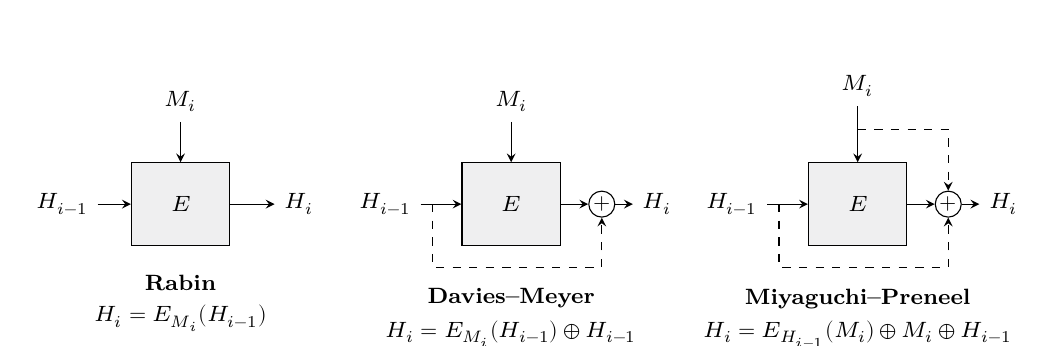
\begin{tikzpicture}[font=\footnotesize, >=stealth,
  enc/.style={draw, fill=gray!12, minimum width=1.25cm, minimum height=1.05cm, align=center},
  xo/.style={draw, circle, inner sep=0pt, minimum size=0.33cm}]
% Rabin
\node[enc] (e1) at (0,0) {$E$};
\node (m1) at (0,1.3) {$M_i$}; \node (h1) at (-1.5,0) {$H_{i-1}$}; \node (o1) at (1.5,0) {$H_i$};
\draw[->] (m1) -- (e1); \draw[->] (h1) -- (e1); \draw[->] (e1) -- (o1);
\node at (0,-1.0) {\textbf{Rabin}};
\node at (0,-1.45) {$H_i = E_{M_i}(H_{i-1})$};
% Davies-Meyer
\begin{scope}[xshift=4.2cm]
\node[enc] (e2) at (0,0) {$E$};
\node (m2) at (0,1.3) {$M_i$}; \node (h2) at (-1.6,0) {$H_{i-1}$};
\node[xo] (x2) at (1.15,0) {$+$}; \node (o2) at (1.85,0) {$H_i$};
\draw[->] (m2) -- (e2); \draw[->] (h2) -- (e2); \draw[->] (e2) -- (x2); \draw[->] (x2) -- (o2);
\draw[->, dashed] (-1.0,0) |- (0.6,-0.8) -| (x2);
\node at (0,-1.2) {\textbf{Davies--Meyer}};
\node at (0,-1.65) {$H_i = E_{M_i}(H_{i-1}) \oplus H_{i-1}$};
\end{scope}
% Miyaguchi-Preneel
\begin{scope}[xshift=8.6cm]
\node[enc] (e3) at (0,0) {$E$};
\node (m3) at (0,1.5) {$M_i$}; \node (h3) at (-1.6,0) {$H_{i-1}$};
\node[xo] (x3) at (1.15,0) {$+$}; \node (o3) at (1.85,0) {$H_i$};
\draw[->] (m3) -- (e3); \draw[->] (h3) -- (e3); \draw[->] (e3) -- (x3); \draw[->] (x3) -- (o3);
\draw[->, dashed] (-1.0,0) |- (0.6,-0.8) -| (x3);
\draw[->, dashed] (0,0.95) -| (x3);
\node at (0,-1.2) {\textbf{Miyaguchi--Preneel}};
\node at (0,-1.65) {$H_i = E_{H_{i-1}}(M_i) \oplus M_i \oplus H_{i-1}$};
\end{scope}
\end{tikzpicture}
\end{center}
In the Rabin and Davies--Meyer pictures the block $M_i$ enters as the \emph{key} (from above) and $H_{i-1}$ as the plaintext; in Miyaguchi--Preneel it is the other way round: $M_i$ is the plaintext and $H_{i-1}$ the key (slide 45). Dashed lines are the feed-forward XORs.

\textbf{Rabin scheme.} Rabin plugs a block cipher directly into Merkle--Damg\aa rd: the message block is used as the key, the previous digest as the plaintext, and the ciphertext is the new digest, $H_i = E_{M_i}(H_{i-1})$. The digest size equals the cipher's block size, so with DES the digest is only 64 bits. Although the scheme is very simple, it is subject to a \textbf{meet-in-the-middle attack}. Because Eve knows every key (the message blocks are her choice), each step can be run \emph{backwards}: $H_{i-1} = D_{M_i}(H_i)$. To forge a message with a given digest $H_t$, she encrypts forward from $H_0$ with about $2^{m/2}$ random choices of the first half of the blocks, stores the intermediate values, then decrypts backward from $H_t$ with about $2^{m/2}$ random choices of the second half, and looks for a common intermediate value. A match gives a full message with digest $H_t$ after only about $2 \times 2^{m/2}$ operations instead of $2^m$; for DES that is about $2^{32}$, which is feasible.

\textbf{Davies--Meyer scheme.} Davies--Meyer is the Rabin scheme plus a \textbf{feed-forward}: the previous digest is XORed onto the cipher output, $H_i = E_{M_i}(H_{i-1}) \oplus H_{i-1}$. Since $H_{i-1}$ now appears both inside the encryption and in the XOR, knowing $H_i$ and $M_i$ no longer lets Eve compute $H_{i-1}$ by decryption, so the backward half of the meet-in-the-middle attack is blocked. This is the protection the slide refers to.

\textbf{Matyas--Meyer--Oseas scheme} (Forouzan, not on the slides). This is the dual of Davies--Meyer: the previous digest is the key (passed through a function $g$ that adapts it to the key size) and the message block is the plaintext, with the block fed forward, $H_i = E_{g(H_{i-1})}(M_i) \oplus M_i$. It is useful when the key and block sizes of the cipher are equal.

\textbf{Miyaguchi--Preneel scheme.} To make the algorithm stronger, the plaintext, the cipher key and the ciphertext are all XORed together to create the new digest: $H_i = E_{H_{i-1}}(M_i) \oplus M_i \oplus H_{i-1}$. It is Matyas--Meyer--Oseas with the chaining value also fed forward. Whirlpool (below) is built on this scheme.

\subsection{SHA-512: overview and parameters \hot}
\asked{End-sem 2025--26 Q5 (7 marks): explain SHA-512 design: message preparation, word expansion, compression function, structure of each round.}
\likely{``Explain SHA-512 with a block diagram: padding, word expansion, round function'' (4--5 marks).}

SHA-512 is the member of the SHA-2 family with the longest digest. It follows the Merkle--Damg\aa rd scheme exactly: the message is padded and given a length field, split into 1024-bit blocks, and each block is fed with the previous 512-bit digest into a compression function; the output of the last block is the 512-bit digest.

\begin{center}
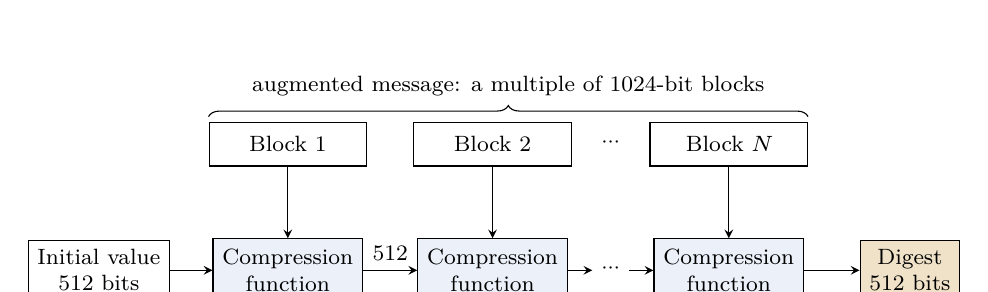
\begin{tikzpicture}[font=\footnotesize, >=stealth,
  blk/.style={draw, minimum width=2.0cm, minimum height=0.55cm},
  cf/.style={draw, fill=acc!8, minimum width=1.9cm, minimum height=0.8cm, align=center}]
\node[blk] (b1) at (0,1.6) {Block 1};
\node[blk] (b2) at (2.6,1.6) {Block 2};
\node (bd) at (4.1,1.6) {$\cdots$};
\node[blk] (bn) at (5.6,1.6) {Block $N$};
\draw[decorate,decoration={brace,amplitude=4pt}] ([yshift=2pt]b1.north west) -- node[above=4pt]{augmented message: a multiple of 1024-bit blocks} ([yshift=2pt]bn.north east);
\node[draw, align=center] (iv) at (-2.4,0) {Initial value\\512 bits};
\node[cf] (c1) at (0,0) {Compression\\function};
\node[cf] (c2) at (2.6,0) {Compression\\function};
\node (cd) at (4.1,0) {$\cdots$};
\node[cf] (cn) at (5.6,0) {Compression\\function};
\node[draw, fill=gold!20, align=center] (dg) at (7.9,0) {Digest\\512 bits};
\draw[->] (b1) -- (c1); \draw[->] (b2) -- (c2); \draw[->] (bn) -- (cn);
\draw[->] (iv) -- (c1); \draw[->] (c1) -- node[above]{512} (c2); \draw[->] (c2) -- (cd); \draw[->] (cd) -- (cn); \draw[->] (cn) -- (dg);
\end{tikzpicture}
\end{center}

SHA-512 is \textbf{word oriented}: a word is 64 bits. Each 1024-bit message block is 16 words, and the 512-bit digest is 8 words, named $A, B, C, D, E, F, G, H$. The parameters are: maximum message length $2^{128} - 1$ bits, block 1024 bits, digest 512 bits, 80 rounds per block, 64-bit words, 80 round constants $K_0, \dots, K_{79}$, and 80 expanded words $W_0, \dots, W_{79}$ per block.

\subsection{SHA-512: padding and length field \new}
\likely{``Compute the number of padding bits for a message of length $L$; is padding needed if the length is already a multiple of 1024?'' (2--3 marks).}

Before processing, Merkle--Damg\aa rd requires the message to be a whole number of blocks, with its length recorded at the end. SHA-512 therefore appends two things to the original message $M$: \textbf{padding}, which is a single 1 bit followed by as many 0 bits as needed, and a \textbf{128-bit length field} holding $|M|$ as an unsigned integer (this is why the maximum message length is $2^{128} - 1$). The total $|M| + |P| + 128$ must be a multiple of 1024, so
\[
|M| + |P| + 128 \equiv 0 \pmod{1024} \quad\Longrightarrow\quad \boxed{\,|P| = (-|M| - 128) \bmod 1024\,}, \qquad 0 \le |P| \le 1023 .
\]
Since the mod gives a value from 0 to 1023, the padding is always less than one block.

\begin{worked}[: padding (Forouzan Example 12.1)]
\textbf{Q.} What is the number of padding bits if the length of the original message is 2590 bits?

\textbf{A.} $|P| = (-2590 - 128) \bmod 1024 = (-2718) \bmod 1024$. Since $-2718 + 3 \times 1024 = 354$, $|P| = \mathbf{354}$ bits: a 1 followed by 353 zeros.\\
\emph{Check}: $2590 + 354 + 128 = 3072 = 3 \times 1024$, so the augmented message is exactly 3 blocks.
\end{worked}

\begin{worked}[: padding, new example]
\textbf{Q.} A message of 5000 bits is hashed with SHA-512. Find the number of padding bits, the number of blocks, and the content of the length field.

\textbf{A.} $|P| = (-5000 - 128) \bmod 1024 = (-5128) \bmod 1024 = -5128 + 6 \times 1024 = \mathbf{1016}$ bits (a 1 followed by 1015 zeros).\\
Total $= 5000 + 1016 + 128 = 6144 = \mathbf{6}$ \textbf{blocks}. The 128-bit length field holds $5000 = $ \ttx{1388} in hex, i.e.\ 115 zero bits followed by \ttx{1001110001000}.\\
\emph{Check}: $6144 / 1024 = 6$ exactly.
\end{worked}

\textbf{Edge cases (Forouzan Examples 12.2--12.3).} A message whose length is \emph{already} a multiple of 1024 still needs padding, because the length field must be added: for $|M| = 1024$, $|P| = (-1152) \bmod 1024 = 896$ and the result is 2 blocks. The formula gives the \textbf{minimum} padding $|P| = 0$ when $|M| \equiv 896 \pmod{1024}$ (the message plus the length field already fill the block) and the \textbf{maximum} $|P| = 1023$ when $|M| \equiv 897 \pmod{1024}$. In the actual standard (FIPS 180) the single 1 bit is always appended, so the padding is at least 1 bit; for $|M| \equiv 896$ this forces a full extra block of 1024 padding bits. A short check of the real rule: the 24-bit message ``abc'' gets $(-24 - 128) \bmod 1024 = 872$ padding bits and fits in one block.

\begin{trap}[: padding arithmetic]
Take the mod of a negative number correctly: add multiples of 1024 until the value lies in $0$--$1023$. Do not forget the 128-bit length field (SHA-1 and SHA-256 use a 64-bit field and 512-bit blocks, giving $|P| = (-|M| - 64) \bmod 512$).
\end{trap}

\subsection{SHA-512: word expansion and the compression function \new}

\textbf{Word expansion.} Each round uses one 64-bit word, but a block has only 16 words, so the block is expanded to 80 words $W_0, \dots, W_{79}$. The first 16 are the block itself; each later word mixes four earlier ones:
\[
W_i = W_{i-16} \oplus \mathrm{RotShift}_{1\text{-}8\text{-}7}(W_{i-15}) \oplus W_{i-7} \oplus \mathrm{RotShift}_{19\text{-}61\text{-}6}(W_{i-2}), \qquad 16 \le i \le 79,
\]
\[
\mathrm{RotShift}_{l\text{-}m\text{-}n}(x) = \mathrm{RotR}_l(x) \oplus \mathrm{RotR}_m(x) \oplus \mathrm{ShL}_n(x),
\]
where $\mathrm{RotR}_i(x)$ rotates $x$ right by $i$ bits (bits leaving on the right re-enter on the left) and $\mathrm{ShL}_i(x)$ shifts $x$ left by $i$ bits, filling with 0s (bits leaving are lost). This is the slides' (Forouzan's) form; see the correction box for the standard's exact operations. Since every later word depends on several earlier ones, a change in one message bit spreads into many of the 80 words.

\textbf{Initial values and constants.} The eight words of $H_0$ are the first 64 bits of the fractional parts of the square roots of the first eight primes (2 to 19); for example $A_0 = $ \ttx{6A09E667F3BCC908} from $\sqrt 2$. The 80 round constants $K_0, \dots, K_{79}$ are the first 64 bits of the fractional parts of the cube roots of the first 80 primes (2 to 409); for example $K_0 = $ \ttx{428A2F98D728AE22} from $\sqrt[3]{2}$. Taking them from irrational numbers shows that the designers hid no trapdoor in the constants (``nothing up my sleeve'' numbers).

\textbf{Compression function.} Processing one block takes 80 rounds. At the start, the eight digest words from the previous block (or the IV) are saved in eight temporary variables. Round $i$ mixes the current $A, \dots, H$ with the word $W_i$ and the constant $K_i$ and produces a new set of eight words. After round 79, the saved values are added to the outputs word by word modulo $2^{64}$; this \textbf{final adding} produces the digest that is passed to the next block (or is the final digest). The final adding is a feed-forward, exactly like Davies--Meyer, and it makes the compression function impossible to run backwards.

\textbf{Structure of each round.} Six of the eight words are simply moved one place right, and only two new words are computed, using two mixers (every $+$ here is addition modulo $2^{64}$):
\[
T_1 = H + \mathrm{Conditional}(E, F, G) + \mathrm{Rotate}(E) + W_i + K_i, \qquad T_2 = \mathrm{Majority}(A, B, C) + \mathrm{Rotate}(A),
\]
\[
H \leftarrow G,\; G \leftarrow F,\; F \leftarrow E,\; E \leftarrow D + T_1,\; D \leftarrow C,\; C \leftarrow B,\; B \leftarrow A,\; A \leftarrow T_1 + T_2 .
\]
The three functions are bitwise (except Rotate, which moves bits within the word):
\begin{itemize}[nosep]
  \item $\mathrm{Majority}(x, y, z) = (x \wedge y) \oplus (y \wedge z) \oplus (z \wedge x)$: each output bit is the majority value of the three input bits.
  \item $\mathrm{Conditional}(x, y, z) = (x \wedge y) \oplus (\overline{x} \wedge z)$: each bit of $x$ acts as a selector, taking the bit of $y$ where $x = 1$ and the bit of $z$ where $x = 0$ (``if $x$ then $y$ else $z$'').
  \item $\mathrm{Rotate}(x) = \mathrm{RotR}_{28}(x) \oplus \mathrm{RotR}_{34}(x) \oplus \mathrm{RotR}_{39}(x)$.
\end{itemize}

\begin{center}
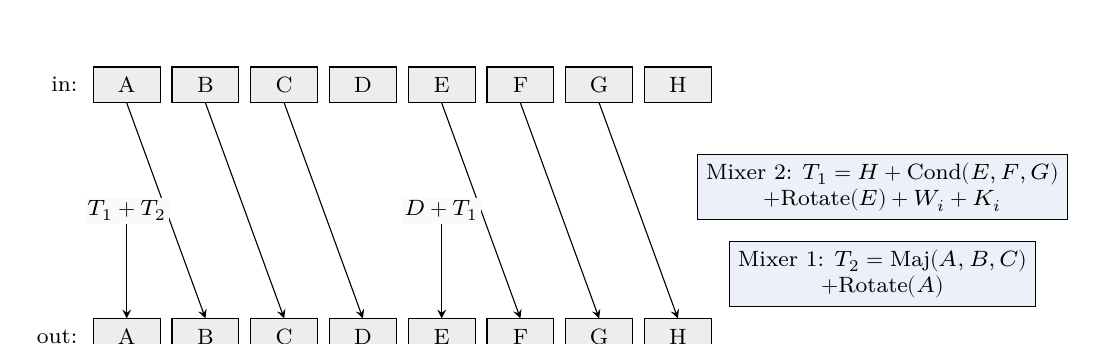
\begin{tikzpicture}[font=\footnotesize, >=stealth,
  reg/.style={draw, fill=gray!15, minimum width=0.85cm, minimum height=0.45cm, inner sep=1pt},
  mix/.style={draw, fill=acc!8, align=center, inner sep=3pt}]
\foreach \n [count=\i] in {A,B,C,D,E,F,G,H} {
  \node[reg] (t\n) at (\i*1.0,3.2) {\n};
  \node[reg] (b\n) at (\i*1.0,0) {\n};
}
\foreach \a/\b in {A/B,B/C,C/D,E/F,F/G,G/H} \draw[->] (t\a.south) -- (b\b.north);
\node[mix] (m2) at (10.6,1.9) {Mixer 2: $T_1 = H + \mathrm{Cond}(E,F,G)$\\$+ \mathrm{Rotate}(E) + W_i + K_i$};
\node[mix] (m1) at (10.6,0.8) {Mixer 1: $T_2 = \mathrm{Maj}(A,B,C)$\\$+ \mathrm{Rotate}(A)$};
\node[font=\footnotesize, fill=white, inner sep=1pt] (xa) at (1.0,1.6) {$T_1 + T_2$};
\node[font=\footnotesize, fill=white, inner sep=1pt] (xe) at (5.0,1.6) {$D + T_1$};
\draw[->] (xa) -- (bA.north); \draw[->] (xe) -- (bE.north);
\node[left=2pt of tA] {in:};
\node[left=2pt of bA] {out:};
\end{tikzpicture}
\end{center}
In Forouzan's notation the new $A$ is called $X$ and the new $E$ is $Y$. Because $A$ and $E$ change every round and the other six words are shifted, every input word affects all eight words within a few rounds.

\begin{mustknow}[: SHA-512 in numbers]
Block 1024 bits $=$ 16 words of 64 bits; digest 512 bits $=$ 8 words $A$--$H$; 80 rounds; 80 words $W_0$--$W_{79}$; 80 constants $K_i$; length field 128 bits; $|P| = (-|M| - 128) \bmod 1024$; max message $2^{128} - 1$ bits; final adding modulo $2^{64}$.
\end{mustknow}

\subsection{Exercises on the SHA-512 operations \new}
\likely{One of the slide exercises (RotR, ShL, Conditional, Majority, Rotate) on given hex words.}

The slide exercises use a \textbf{128-bit} $x$ (real SHA-512 words are 64 bits) and work in hex: a rotation or shift by 12 bits moves the string by 3 hex digits. All results below were recomputed.
\[
x = \texttt{1234 5678 ABCD 2345 3456 5678 ABCD 2468}
\]

\begin{worked}[: RotR, ShL, Conditional, Majority, Rotate (slides 52--56)]
\textbf{RotR$_{12}(x)$.} Rotate right by 12 bits $=$ 3 hex digits: the last three digits \ttx{468} move to the front.\\
\ttx{4681 2345 678A BCD2 3453 4565 678A BCD2}

\textbf{ShL$_{12}(x)$.} Shift left by 3 hex digits: the first three digits \ttx{123} are lost and three 0 digits enter on the right.\\
\ttx{4567 8ABC D234 5345 6567 8ABC D246 8000}

\textbf{Conditional$(x, y, z)$} with $y = $ \ttx{2234 5678 \dots}, $z = $ \ttx{3234 5678 \dots} (the three words differ only in the first digit). For the first digit, $x = 0001$ selects $y$ where $x = 1$ and $z$ where $x = 0$: $(0001 \wedge 0010) \oplus (1110 \wedge 0011) = 0000 \oplus 0010 = 0010 = 2$. For every other digit the three inputs are equal, and Conditional of three equal digits is that digit.\\
Result: \ttx{2234 5678 ABCD 2345 3456 5678 ABCD 2468}

\textbf{Majority$(x, y, z)$}, same $x, y, z$. First digit: $(0001 \wedge 0010) \oplus (0010 \wedge 0011) \oplus (0011 \wedge 0001) = 0000 \oplus 0010 \oplus 0001 = 0011 = 3$. The other digits are unchanged.\\
Result: \ttx{3234 5678 ABCD 2345 3456 5678 ABCD 2468}

\textbf{Rotate$(x) = \mathrm{RotR}_{28}(x) \oplus \mathrm{RotR}_{34}(x) \oplus \mathrm{RotR}_{39}(x)$.} First the three rotations, then the XOR:\\[2pt]
{\small
\begin{tabular}{@{}ll@{}}
$\mathrm{RotR}_{28}(x)$ & \ttx{BCD2 4681 2345 678A BCD2 3453 4565 678A}\\
$\mathrm{RotR}_{34}(x)$ & \ttx{2AF3 491A 048D 159E 2AF3 48D1 4D15 959E}\\
$\mathrm{RotR}_{39}(x)$ & \ttx{F157 9A48 D024 68AC F157 9A46 8A68 ACAC}\\
\midrule
Rotate$(x)$ & \ttx{6776 95D3 F7EC 1AB8 6776 E6C4 8218 5EB8}
\end{tabular}}\\[2pt]
$\mathrm{RotR}_{28}$ is a rotation by 7 hex digits, so it can be done digit-wise; $\mathrm{RotR}_{34}$ and $\mathrm{RotR}_{39}$ are not multiples of 4 and must be done in binary.
\end{worked}

\begin{worked}[: new exercise on 16-bit and 64-bit words]
\textbf{Q.} (a) For the 16-bit words $x = $ \ttx{F0F0}, $y = $ \ttx{AAAA}, $z = $ \ttx{5555}, find Conditional$(x, y, z)$ and Majority$(x, y, z)$. (b) For the 64-bit word $w = $ \ttx{0123 4567 89AB CDEF}, find $\mathrm{RotR}_8(w)$ and $\mathrm{ShL}_8(w)$.

\textbf{A.} (a) Conditional takes $y$ where $x$ is 1 and $z$ where $x$ is 0. $x \wedge y = $ \ttx{A0A0}, $\overline x \wedge z = $ \ttx{0F0F} $\wedge$ \ttx{5555} $= $ \ttx{0505}; Conditional $= $ \ttx{A0A0} $\oplus$ \ttx{0505} $= \mathbf{A5A5}$.\\
Majority: $x \wedge y = $ \ttx{A0A0}, $y \wedge z = $ \ttx{0000} (since $z = \overline y$), $z \wedge x = $ \ttx{5050}; XOR $= \mathbf{F0F0}$. This equals $x$, as it must: $y$ and $z$ disagree in every bit, so $x$ always casts the deciding vote.\\
(b) 8 bits $=$ 2 hex digits. $\mathrm{RotR}_8(w) = $ \ttx{EF01 2345 6789 ABCD} (\ttx{EF} wraps to the front); $\mathrm{ShL}_8(w) = $ \ttx{2345 6789 ABCD EF00} (\ttx{01} is lost, \ttx{00} enters).
\end{worked}

\subsection{Whirlpool}
Whirlpool, designed by Rijmen and Barreto and selected by the NESSIE project (New European Schemes for Signatures, Integrity, and Encryption), is an iterated hash function based on the \textbf{Miyaguchi--Preneel} scheme, in which the compression function is a block cipher: $H_i = E_{H_{i-1}}(M_i) \oplus M_i \oplus H_{i-1}$. The cipher, called W, is a \textbf{modified AES} tailored for this purpose.

\textbf{Parameters.} Block size 512 bits, digest 512 bits, cipher key 512 bits (the previous digest), initial value $H_0$ all 0s, and maximum message length $2^{256} - 1$ bits. The message is padded (a 1 followed by 0s) to an \emph{odd} multiple of 256 bits and then a \textbf{256-bit length field} is appended; an odd multiple of 256 plus 256 is an even multiple, i.e.\ a multiple of 512. For example, $|M| = 1000$ needs $|P| = (-1000 - 256) \bmod 512 = 280$ padding bits, since $1000 + 280 = 1280 = 5 \times 256$ (odd) and $1280 + 256 = 1536 = 3 \times 512$.

\textbf{How the Whirlpool cipher differs from AES.} It uses the same four kinds of transformation, but on a larger state and with all rounds alike:
\begin{itemize}[nosep]
  \item The block and key are 512 bits, held as an $8 \times 8$ matrix of bytes (AES: 128 bits as $4 \times 4$).
  \item There are 10 rounds, each with SubBytes, \textbf{ShiftColumns} (column $j$ is rotated down by $j$ positions, instead of AES's ShiftRows), \textbf{MixRows} (each row is multiplied by a fixed $8 \times 8$ circulant matrix, instead of AES's MixColumns) and AddRoundKey.
  \item Arithmetic is in GF$(2^8)$ with modulus $x^8 + x^4 + x^3 + x^2 + 1$ (AES uses $x^8 + x^4 + x^3 + x + 1$), and the S-box is built from smaller 4-bit boxes.
  \item The round keys are generated by running the same round function on the key, with round constants taken from the S-box in place of a key, instead of AES's separate key-expansion routine.
\end{itemize}

\begin{fixbox}
\begin{itemize}[nosep]
  \item Slide 27: ``$0.69 \times 2^{34}$ seconds or more than 500 years''. In fact $0.69 \times 2^{34}$ s $\approx 376$ years ($2^{34}$ s alone is $\approx 544$ years). The conclusion (secure against preimage attacks) stands.
  \item Slides 54--55 swap the binary for the first digit: Conditional$(0001, 0010, 0011) = 0010 = 2$ and Majority$(0001, 0010, 0011) = 0011 = 3$; the slides print 0011 for Conditional and 0010 for Majority, though the hex results 2 and 3 are right. Both slides also label the third word $x$ instead of $z$.
  \item The exercise $x$ (slides 52--56) is 128 bits, though real SHA-512 words are 64 bits; the rotations on the slides are done on 128 bits, and the results above follow the slides.
  \item Slide 11 prints Problem 4 as $P \approx 1 - e^{-k^2/2N}$; that formula would give $k = 1.18\sqrt N$. The correct one is $P \approx 1 - e^{-k^2/N}$ (as on slide 35), which gives $k = 0.83\sqrt N = 16$.
  \item Slide 40 lists SHA under the ``block cipher'' approach. Forouzan classifies MD and SHA as compression functions \emph{made from scratch} and Rabin, Davies--Meyer, Matyas--Meyer--Oseas and Miyaguchi--Preneel as block-cipher based; write it that way in the exam.
  \item Slides 48 and 51 (from Forouzan) simplify the standard: in FIPS 180 the word expansion uses addition modulo $2^{64}$ and a \emph{right} shift (SHR), not XOR and ShL, and Rotate$(E)$ uses $\mathrm{RotR}_{14} \oplus \mathrm{RotR}_{18} \oplus \mathrm{RotR}_{41}$, not 28-34-39. The slide's ``ShL\dots padding the left by 0s'' is self-contradictory (a left shift fills on the right). For the exam, use the slide formulas.
\end{itemize}
\end{fixbox}

% College Lecture 15 (message authentication, digital signatures; 48 slides) + Forouzan 11.3, ch. 13, Stallings (MACs, HMAC, CMAC, DSS).
% Every number recomputed by script (scratchpad/w20/v1.py ... v9.py, ec.py, lenext.py): RSA/ElGamal/DSS/Schnorr/ECDSA runs, attacks, HMAC, CMAC.
\section{Message Authentication: MDC, MAC, HMAC and CMAC}\label{sec:mac}
\usetikzlibrary{decorations.pathreplacing}
\tikzset{
  dsgop/.style={draw, fill=white, align=center, inner sep=3pt, minimum height=0.62cm, font=\small},
  dsgdia/.style={draw, diamond, aspect=2.3, inner sep=0.5pt, fill=white, font=\small},
  dsgblk/.style={draw, fill=gray!15, minimum height=0.55cm, inner sep=2pt, font=\small},
  dsgtag/.style={draw, fill=black, text=white, font=\small\bfseries, inner sep=3pt},
  dsgzone/.style={draw, dashed, fill=gray!8}
}

\subsection{Why a digest does not authenticate: MDC versus MAC \new}
\likely{``Why can a message digest not provide message authentication? Differentiate MDC and MAC with diagrams'' (3--4 marks).}

A message digest guarantees \textbf{integrity}: if Alice sends $M$ and Bob recomputes $h(M)$, any change to $M$ produces a different digest (\S\ref{sec:integrity}). It does \emph{not} tell Bob who created the message. The hash function is public and needs no secret, so Eve can write her own message $M'$, compute $h(M')$ and send the pair $(M', h(M'))$; Bob's comparison succeeds, because the pair is internally consistent, and he has no way of telling it from a pair made by Alice. To prove that the message comes from Alice and not an impostor (\textbf{message authentication}, also called \textbf{data-origin authentication}), the check value must depend on something that only Alice and Bob know.

\textbf{Modification detection code (MDC).} A digest made by a keyless cryptographic hash function is called an MDC, because it can only detect modification. The MDC itself must therefore travel over a \emph{safe} channel (a channel immune to change), while the message may travel over an insecure one. Bob hashes the received message and compares the result with the MDC from the safe channel; if they are equal the message is accepted, otherwise rejected.

\begin{center}
\begin{tikzpicture}[font=\small, >=Stealth]
\fill[gray!8] (0,-1.9) rectangle (3.8,1.1); \draw[dashed] (0,-1.9) rectangle (3.8,1.1);
\fill[gray!8] (7.6,-1.9) rectangle (15.8,1.1); \draw[dashed] (7.6,-1.9) rectangle (15.8,1.1);
\node[above right] at (0,1.1) {\textbf{Alice}}; \node[above left] at (15.8,1.1) {\textbf{Bob}};
\node[dsgblk] (m) at (0.9,0.5) {$M$};
\node[dsgop] (h) at (0.9,-0.7) {Hash};
\node[dsgtag] (mdc) at (2.7,-0.7) {MDC};
\draw[->] (m) -- (h); \draw[->] (h) -- (mdc);
\node[dsgblk] (mb) at (8.3,0.5) {$M$};
\node[dsgop] (hb) at (10.2,0.5) {Hash};
\node[dsgtag] (mdcb) at (8.5,-0.7) {MDC};
\node[dsgdia] (cmp) at (12.4,-0.7) {Same?};
\draw[->] (m) -- (mb); \node[above] at (5.7,0.5) {insecure channel};
\draw[->] (mdc) -- (mdcb); \node[below, align=center, font=\footnotesize] at (5.7,-0.75) {safe channel\\(immune to change)};
\draw[->] (mb) -- (hb); \draw[->] (hb) -| (cmp);
\draw[->] (mdcb) -- (cmp);
\draw[->] (cmp) -- node[above]{yes} (14.6,-0.7) node[right]{accept};
\draw[->] (cmp.south) -- ++(0,-0.45) node[right, font=\footnotesize]{no: reject};
\end{tikzpicture}
\end{center}

\textbf{Message authentication code (MAC).} A MAC removes the need for a safe channel by mixing a \textbf{shared secret key} $K$ into the digest. Alice computes $\mathrm{MAC} = h(K \,|\, M)$, where $|$ denotes concatenation, and sends $M$ and the MAC together over the insecure channel. Bob separates the two, computes a new MAC from the received message and his copy of $K$, and compares it with the received MAC. \imp{If the two MACs match, the message is authentic (it was made by a holder of $K$) and has not been modified.} Eve can still change $M$, but without $K$ she cannot compute the MAC that goes with the new message, so the change is detected.

\begin{center}
\begin{tikzpicture}[font=\small, >=Stealth]
\fill[gray!8] (-0.9,-1.9) rectangle (3.8,1.3); \draw[dashed] (-0.9,-1.9) rectangle (3.8,1.3);
\fill[gray!8] (7.6,-1.9) rectangle (15.8,1.3); \draw[dashed] (7.6,-1.9) rectangle (15.8,1.3);
\node[above right] at (-0.9,1.3) {\textbf{Alice}}; \node[above left] at (15.8,1.3) {\textbf{Bob}};
\node[dsgblk] (m) at (0.9,0.5) {$M$};
\node[dsgop] (h) at (0.9,-0.7) {Hash};
\node (k) at (-0.45,-0.7) {$K$}; \draw[->] (k) -- (h);
\node[dsgtag] (mac) at (2.4,-0.7) {MAC};
\node[draw, dashed, fill=white, align=center, inner sep=2pt] (pkt) at (3.2,0.2) {$M$\\[-1pt]\colorbox{black}{\textcolor{white}{\scriptsize MAC}}};
\draw[->] (m) -- (h); \draw[->] (h) -- (mac); \draw[->] (mac) -| (pkt); \draw[->] (m) -- (m -| pkt.west);
\node[draw, dashed, fill=white, align=center, inner sep=2pt] (pkb) at (8.3,0.2) {$M$\\[-1pt]\colorbox{black}{\textcolor{white}{\scriptsize MAC}}};
\draw[->] (pkt) -- (pkb); \node[above] at (5.7,0.2) {insecure channel: $M + \mathrm{MAC}$};
\node[dsgop] (hb) at (10.4,0.2) {Hash};
\node (kb) at (10.4,0.95) {$K$}; \draw[->] (kb) -- (hb);
\node[dsgdia] (cmp) at (12.6,-0.9) {Same?};
\draw[->] (pkb) -- (hb); \draw[->] (hb) -| node[above, pos=0.3, font=\footnotesize]{new MAC} (cmp);
\draw[->] (pkb.south) |- node[below, pos=0.7, font=\footnotesize]{received MAC} (cmp);
\draw[->] (cmp) -- node[above]{yes} (14.6,-0.9) node[right]{accept};
\draw[->] (cmp.south) -- ++(0,-0.35) node[right, font=\footnotesize]{no: reject};
\end{tikzpicture}
\end{center}

\begin{center}\small
\begin{tabularx}{\textwidth}{@{}l X X@{}}
\toprule
 & MDC (modification detection code) & MAC (message authentication code)\\
\midrule
Computed as & $h(M)$, keyless hash & $h(K \,|\, M)$ (or HMAC, CMAC) with a shared secret key $K$\\
Service & integrity only & integrity \emph{and} data-origin authentication\\
Channel for the code & must be safe (immune to change) & the MAC travels with $M$ over the insecure channel\\
Who can create a valid code & anyone & only holders of $K$ (Alice and Bob)\\
Nonrepudiation & no & no: Bob holds $K$ too, so he could have made the MAC himself\\
\bottomrule
\end{tabularx}
\end{center}
The last row is the reason digital signatures (\S\ref{sec:dsig}) are needed: a MAC convinces Bob, but it cannot convince a judge that Alice, rather than Bob, produced it.

\subsection{Prefix, postfix and envelope MACs from a hash \new}
\likely{``What is a prefix MAC? Why is $h(K|M)$ insecure with an iterated hash?'' (2--3 marks).}

The slide's MAC $h(K \,|\, M)$ is a \textbf{prefix MAC}: the secret key is placed at the beginning of the message before hashing. In a \textbf{postfix MAC} the key is appended at the end, $h(M \,|\, K)$, and the two can be combined into an \textbf{envelope} $h(K \,|\, M \,|\, K)$, with the same key at both ends or two different keys $h(K_1 \,|\, M \,|\, K_2)$. All three look reasonable, but each inherits a weakness from the iterated (Merkle--Damg\aa rd) structure of real hash functions.

\textbf{Length extension breaks the prefix MAC.} In an iterated hash the digest is simply the last chaining value $H_t$, and the computation of $h$ on a longer message just continues from it: $H_{t+1} = f(H_t, X)$. Suppose Eve sees $M$ and its tag $T = h(K \,|\, M)$. She knows the length of $K \,|\, M$ (key lengths are public), so she knows the padding block $P$ that the hash appended. She can therefore take $T$ as the chaining value, run the compression function on an extra block $X$ of her choice (followed by the correct new padding), and obtain
\[
T' = h(K \,|\, M \,|\, P \,|\, X)
\]
without ever knowing $K$. The pair $(M \,|\, P \,|\, X,\ T')$ is a valid message--MAC pair, so Eve has forged a MAC on a longer message that begins with Alice's message (we checked this on SHA-256 by script: the forged tag equals the true $h(K \,|\, M \,|\, P \,|\, X)$).
\begin{center}
\begin{tikzpicture}[font=\small, >=Stealth]
\node[draw, minimum height=0.6cm] (iv) at (0,0) {IV};
\node[dsgop] (f1) at (1.7,0) {$f$}; \node[dsgop] (f2) at (3.3,0) {$f$}; \node (dd) at (4.6,0) {$\cdots$}; \node[dsgop] (ft) at (5.9,0) {$f$};
\node[dsgtag] (t) at (7.6,0) {$T$};
\node[dsgop, fill=warn!12] (fx) at (9.6,0) {$f$}; \node[draw, fill=gold!25, inner sep=3pt] (t2) at (11.5,0) {$T'$};
\node[dsgblk] (b1) at (1.7,1.1) {$K$}; \node[dsgblk] (b2) at (3.3,1.1) {$M_1$}; \node[dsgblk] (bt) at (5.9,1.1) {$M_t \,|\, P$};
\node[dsgblk, fill=warn!20] (bx) at (9.6,1.1) {$X \,|\, P'$};
\draw[->] (iv) -- (f1); \draw[->] (f1) -- (f2); \draw[->] (f2) -- (dd); \draw[->] (dd) -- (ft); \draw[->] (ft) -- (t); \draw[->] (t) -- (fx); \draw[->] (fx) -- (t2);
\foreach \a/\b in {b1/f1, b2/f2, bt/ft, bx/fx} \draw[->] (\a) -- (\b);
\draw[decorate, decoration={brace, mirror, amplitude=4pt}] (0.9,-0.5) -- node[below=4pt, font=\footnotesize]{computed by Alice: $T = h(K \,|\, M)$, sent with $M$} (7.9,-0.5);
\draw[decorate, decoration={brace, mirror, amplitude=4pt}] (8.9,-0.5) -- node[below=4pt, font=\footnotesize, align=center]{Eve, from $T$ alone: valid tag on $M \,|\, P \,|\, X$} (12.0,-0.5);
\end{tikzpicture}
\end{center}

\textbf{Postfix MAC.} Here the key comes last, so length extension does not work (Eve cannot hash past the unknown key). But if Eve finds an ordinary collision of the keyless hash, $h(M) = h(M')$ with $M$ and $M'$ of the same block length, the chaining values before the key are equal, so $h(M \,|\, K) = h(M' \,|\, K)$ for \emph{every} key. The collision is found offline with about $2^{n/2}$ work (birthday attack), after which a MAC on $M$ is also a MAC on $M'$. The envelope with two keys blocks both tricks, and the cleanest standard solution is the nested MAC (HMAC) below.

\subsection{Security of a MAC \new}
\likely{``How can Eve forge a MAC? On what does its security depend?'' (2--3 marks).}

Suppose Eve has intercepted $M$ and $h(K \,|\, M)$ and wants to forge a message without knowing $K$. The slide lists three possible cases.
\begin{enumerate}[leftmargin=1.6em]
  \item \textbf{Exhaustive key search.} If the key is short, Eve prepends every possible key $K'$ to $M$ and hashes $K' \,|\, M$ until the result equals the intercepted MAC. She then knows the key and can replace the message with any forged message and a correct MAC. The cost is about $2^k$ hash computations for a $k$-bit key, so the key must be long (128 bits or more).
  \item \textbf{Preimage attack.} Since the key is normally too long for exhaustive search, Eve can instead attack the hash: she runs a preimage attack until she finds an $X$ with $h(X)$ equal to the intercepted MAC. Because $X = K \,|\, M$ and she knows $M$, the front of $X$ is the key, which she can then use to forge. This costs about $2^n$ for an $n$-bit digest (\S\ref{sec:integrity}), so the MAC is only as strong as the preimage resistance of $h$.
  \item \textbf{Forging from known pairs.} Given some pairs of messages and their MACs, Eve may be able to manipulate them into a new message with a valid MAC without finding the key at all. Length extension of the prefix MAC is exactly such an attack, and the CBC-MAC splice below is another.
\end{enumerate}
\textbf{Conclusion (slide 7).} \imp{The security of a MAC depends on the security of the underlying hash algorithm} (or block cipher), and on its construction. A brute-force forger needs the smaller of $2^k$ (key search) and $2^n$ (guessing a valid tag), which is why both the key and the tag must be long; the construction must in addition leave no algebraic shortcut such as length extension.

\subsection{Nested MAC and HMAC \hot\new}
\likely{``Explain HMAC with a block diagram; what are ipad and opad; why are two hashes used?'' (5 marks). The most likely MAC question.}

The weakness of $h(K \,|\, M)$ is that its output is the internal state of the hash, which anyone can continue. A \textbf{nested MAC} hides that state by hashing a second time with the key: first $h(K \,|\, M)$ is computed, and then the result is prefixed with the key again and hashed, giving $h\big(K \,|\, h(K \,|\, M)\big)$ (slide 8). Eve can still extend the inner hash in principle, but she never sees it; she sees only the outer digest, and extending \emph{that} produces a hash of $K \,|\, \text{inner} \,|\, P \,|\, X$, which is not the nested MAC of any message. \textbf{HMAC} (hashed MAC, RFC 2104, standardized by NIST as FIPS 198) is the standardized nested MAC; it derives two different keys from $K$ for the two passes.

\textbf{Design objectives (Stallings).} HMAC was designed to use an existing hash function (MD5, SHA-1, SHA-2) without modification, so that available fast code can be used; to allow the hash to be replaced by a newer one when needed; to keep the speed of the hash; to handle keys in a simple way; and to have a security proof relating its strength to that of the hash.

\textbf{Notation.} $H$ is the hash function, with block size $b$ bits (512 for MD5, SHA-1 and SHA-256; 1024 for SHA-512) and digest size $n$ bits. $M$ is the message, split by $H$ into blocks $Y_0, \dots, Y_{L-1}$. $K$ is the secret key; if $|K| > b$ it is first replaced by $H(K)$. $K^+$ is $K$ padded with zeros to exactly $b$ bits (RFC 2104 and FIPS 198 append the zeros at the end; Stallings' figure pads on the left; either way the convention is fixed). The two constant pads are
\[
\mathrm{ipad} = \texttt{00110110} = \texttt{0x36}\ \text{repeated } b/8 \text{ times}, \qquad \mathrm{opad} = \texttt{01011100} = \texttt{0x5C}\ \text{repeated } b/8 \text{ times}.
\]

\begin{mustknow}[: HMAC (FIPS 198, RFC 2104)]
\[
\mathrm{HMAC}(K, M) = H\Big[\, (K^+ \oplus \mathrm{opad}) \;\big\|\; H\big[\, (K^+ \oplus \mathrm{ipad}) \,\|\, M \,\big] \,\Big]
\]
Steps: (1) pad $K$ with zeros to $b$ bits, giving $K^+$; (2) $S_i = K^+ \oplus \mathrm{ipad}$; (3) append $M$ to $S_i$; (4) hash $S_i \| M$ to get the $n$-bit inner digest; (5) $S_o = K^+ \oplus \mathrm{opad}$; (6) append the inner digest to $S_o$ (the hash pads it to a full block); (7) hash $S_o \| \text{inner digest}$; the $n$-bit result is the HMAC.
\end{mustknow}

\begin{center}
\begin{tikzpicture}[font=\small, >=Stealth]
% inner row
\node[draw, minimum height=0.6cm] (k1) at (0,2.4) {$K^+$};
\node[font=\Large, inner sep=0pt] (x1) at (1.6,2.4) {$\oplus$};
\node[font=\footnotesize] (ip) at (1.6,3.4) {ipad $=$ \ttx{36\dots36}};
\node[dsgblk, minimum width=1.35cm] (si) at (3.45,2.4) {$S_i$};
\node[dsgblk, minimum width=1.2cm, anchor=west] (y0) at (si.east) {$Y_0$};
\node[dsgblk, minimum width=1.2cm, anchor=west] (y1) at (y0.east) {$Y_1$};
\node[dsgblk, minimum width=1.0cm, anchor=west, fill=white] (yd) at (y1.east) {$\cdots$};
\node[dsgblk, minimum width=1.35cm, anchor=west] (yl) at (yd.east) {$Y_{L-1}$};
\draw[decorate, decoration={brace, amplitude=4pt}] (y0.north west) -- node[above=4pt, font=\footnotesize]{message $M$} (yl.north east);
\node[below=1pt of si, font=\footnotesize] {$b$ bits};
\node[dsgop, fill=acc!10, minimum width=1.5cm] (h1) at (11.2,2.4) {Hash};
\node[above=2pt of h1, font=\footnotesize] (iv1) {IV ($n$ bits)}; \draw[->] (iv1) -- (h1);
\node[draw, inner sep=3pt] (in) at (13.9,2.4) {inner digest};
\draw[->] (k1) -- (x1); \draw[->] (ip) -- (x1); \draw[->] (x1) -- (si);
\draw[->] (yl) -- (h1); \draw[->] (h1) -- node[above, font=\footnotesize]{$n$} (in);
% outer row
\node[draw, minimum height=0.6cm] (k2) at (0,0) {$K^+$};
\node[font=\Large, inner sep=0pt] (x2) at (1.6,0) {$\oplus$};
\node[font=\footnotesize] (op) at (1.6,-1.0) {opad $=$ \ttx{5C\dots5C}};
\node[dsgblk, minimum width=1.35cm] (so) at (3.45,0) {$S_o$};
\node[dsgblk, minimum width=3.2cm, anchor=west, fill=gold!20] (pd) at (so.east) {inner digest $\|$ pad};
\node[below=1pt of so, font=\footnotesize] {$b$ bits};
\node[dsgop, fill=acc!10, minimum width=1.5cm] (h2) at (11.2,0) {Hash};
\node[below=2pt of h2, font=\footnotesize] (iv2) {IV ($n$ bits)}; \draw[->] (iv2) -- (h2);
\node[dsgtag] (hm) at (13.9,0) {HMAC ($n$ bits)};
\draw[->] (k2) -- (x2); \draw[->] (op) -- (x2); \draw[->] (x2) -- (so);
\draw[->] (pd) -- (h2); \draw[->] (h2) -- (hm);
\draw[->] (in.south) -- ++(0,-0.75) -| (pd.north);
\end{tikzpicture}
\end{center}

\textbf{Why two different pads.} Both pads have exactly four 1-bits per byte ($\texttt{0x36} = \texttt{00110110}$, $\texttt{0x5C} = \texttt{01011100}$), so each XOR flips half of the bits of $K^+$, and the two pads flip different halves ($\texttt{0x36} \oplus \texttt{0x5C} = \texttt{0x6A} = \texttt{01101010}$). After the first compression step, $S_i$ and $S_o$ therefore act as two pseudo-randomly derived, unrelated keys, one for the inner and one for the outer hash, although only one key $K$ is stored.

\textbf{Why two nested hashes.} The inner hash $H[S_i \| M]$ compresses the long message under the secret $S_i$; on its own it would be a prefix MAC and open to length extension. The outer hash takes the inner digest as its \emph{message} and prefixes the second secret $S_o$. Its output reveals nothing usable about the inner chaining state, and extending it only yields a hash of $S_o \| \text{inner} \| \text{pad} \| X$, which is not the HMAC of any message. The outer pass is short (one block), so the protection costs almost nothing.

\textbf{Efficiency.} The blocks $S_i$ and $S_o$ depend only on the key. An implementation computes $f(\mathrm{IV}, S_i)$ and $f(\mathrm{IV}, S_o)$ once per key and stores them as the starting chaining values of the inner and outer hash. After that, each message costs the plain hash of $M$ plus \textbf{one extra compression-function call} (the outer block), so for long messages HMAC runs at practically the speed of the hash itself.

\textbf{Security.} Bellare, Canetti and Krawczyk proved that forging HMAC is as hard as one of two things: computing outputs of the compression function when its IV is secret and random, or finding collisions in the hash when its IV is secret and random. In the second case the birthday attack cannot be run offline, because Eve cannot evaluate the keyed function herself; she must observe about $2^{n/2}$ MACs produced by Alice under one key. For MD5 ($n = 128$) that is $2^{64}$ MACs, more than $2^{72}$ bits of traffic, or about 150\,000 years on a 1 Gbit/s link. Hence \imp{the security of HMAC depends on the cryptographic strength of the underlying hash function}, but HMAC needs much less from the hash than plain hashing does: HMAC-MD5 is still unbroken although MD5 collisions are easy.

\begin{worked}[: one HMAC-SHA-256 computation, block by block]
\textbf{Q.} Describe the computation of HMAC-SHA-256 with key $K = $ ``key'' (3 bytes, \ttx{6B 65 79}) on the 43-byte message $M = $ ``The quick brown fox jumps over the lazy dog''. Give $K^+$, the first bytes of $S_i$ and $S_o$, the number of compression-function calls, and the result.

\textbf{A.} SHA-256 has $b = 512$ bits $= 64$ bytes and $n = 256$ bits.\\
(1) $K^+ = $ \ttx{6B 65 79} followed by 61 zero bytes (64 bytes).\\
(2) $S_i = K^+ \oplus$ \ttx{36 36 \dots}: $\texttt{6B} \oplus \texttt{36} = \texttt{5D}$, $\texttt{65} \oplus \texttt{36} = \texttt{53}$, $\texttt{79} \oplus \texttt{36} = \texttt{4F}$, $\texttt{00} \oplus \texttt{36} = \texttt{36}$, so $S_i = $ \ttx{5D 53 4F 36 36 \dots 36}.\\
(3) $S_o = K^+ \oplus$ \ttx{5C 5C \dots} $=$ \ttx{37 39 25 5C 5C \dots 5C}.\\
(4) Inner hash of $S_i \| M$: $64 + 43 = 107$ bytes; with the \ttx{80} byte and the 8-byte length field it needs $107 + 1 + 8 = 116 \le 128$ bytes, i.e.\ \textbf{2 blocks}.\\
(5) Outer hash of $S_o \| \text{inner}$: $64 + 32 = 96$ bytes, $96 + 9 = 105 \le 128$, again \textbf{2 blocks}.\\
Total 4 compression calls; with $f(\mathrm{IV}, S_i)$ and $f(\mathrm{IV}, S_o)$ cached for this key, only 2 per message.\\
Result (256 bits):\\
\hspace*{1.5em}$\mathrm{HMAC} = $ \ttx{f7bc83f4 30538424 b13298e6 aa6fb143 ef4d59a1 49461759 97479dbc 2d1a3cd8}\\
\emph{Check}: the script's two-pass computation $H[S_o \| H[S_i \| M]]$ equals the library HMAC value.
\end{worked}

\subsection{CBC-MAC (Data Authentication Algorithm) and CMAC \new}
\likely{``Explain CMAC with a diagram; how are the subkeys $k_1, k_2$ generated? Why is plain CBC-MAC insecure for variable-length messages?'' (4--5 marks).}

A MAC can also be built from a block cipher instead of a hash. The idea comes from \textbf{cipher block chaining} (CBC) mode, in which each plaintext block is XORed with the previous ciphertext block before encryption, $C_i = E_K(M_i \oplus C_{i-1})$. Because of the chaining, the last ciphertext block depends on every bit of every message block and on the key, so it can serve as a MAC: only a holder of $K$ can compute it, and any change to any block changes it unpredictably.

\textbf{CBC-MAC / Data Authentication Algorithm (DAA).} The message is split into $N$ blocks of $n$ bits each ($n = 64$ for DES, 128 for AES), the last one padded with zeros. With an all-zero IV, $C_0 = 0^n$,
\[
C_1 = E_K(M_1), \qquad C_i = E_K(M_i \oplus C_{i-1})\ \ (i = 2, \dots, N), \qquad \mathrm{MAC} = \text{leftmost } t \text{ bits of } C_N .
\]
Unlike CBC encryption, only the last block is output; the intermediate $C_i$ are kept secret. The DAA of FIPS PUB 113 is exactly this with DES and a tag of $16 \le t \le 64$ bits.

\textbf{Why plain CBC-MAC fails for variable-length messages.} CBC-MAC is secure when all messages have one fixed length, but not otherwise. Suppose Eve obtains the tag $T = E_K(X)$ of a one-block message $X$. She forms the two-block message $X \,\|\, (X \oplus T)$ and computes its CBC-MAC symbolically:
\[
C_1 = E_K(X) = T, \qquad C_2 = E_K\big((X \oplus T) \oplus C_1\big) = E_K(X \oplus T \oplus T) = E_K(X) = T .
\]
The new message has the \emph{same} tag $T$, so Eve has a valid forgery without knowing $K$ (checked by script with AES). More generally, given $(M, T)$ and $(M', T')$, the splice $M \,\|\, (M'_1 \oplus T) \,\|\, M'_2 \cdots$ has tag $T'$: XORing $T$ into the first block of $M'$ cancels the chaining value that $M$ leaves behind. The root cause is that the last step is an ordinary step, so a tag is also a usable intermediate chaining value. The fix is to make the last step different from the others.

\textbf{CMAC (cipher-based MAC, NIST SP 800-38B).} CMAC (also called OMAC1; Forouzan and the slide call the family ``CMAC or CBC-MAC'') keeps the CBC chain but XORs a secret \textbf{subkey} into the last block, so the input to the final encryption is never a value Eve can predict from earlier tags. One cipher key $K$ is used; the subkeys are derived from it.
\begin{enumerate}[leftmargin=1.6em]
  \item \textbf{Subkey generation.} Encrypt the all-zero block: $L = E_K(0^n)$. Then $k_1 = x \cdot L$ and $k_2 = x \cdot k_1 = x^2 \cdot L$, where multiplication by $x$ is done in GF$(2^n)$ (\S\ref{sec:algebra}). Multiplying by $x$ is a left shift by one bit; if the bit shifted out (the MSB) was 1, the result is reduced by XORing the constant $R_n$:
  \[
  x \cdot L = \begin{cases} L \ll 1 & \text{if } \mathrm{MSB}(L) = 0,\\ (L \ll 1) \oplus R_n & \text{if } \mathrm{MSB}(L) = 1,\end{cases} \qquad R_{128} = 0^{120}\texttt{10000111} = \texttt{0x87},\quad R_{64} = 0^{59}\texttt{11011} = \texttt{0x1B}.
  \]
  The constants are the low terms of the field moduli $x^{128} + x^7 + x^2 + x + 1$ and $x^{64} + x^4 + x^3 + x + 1$: the shifted-out $x^n$ is replaced by its residue.
  \item \textbf{Chaining.} Split $M$ into blocks $M_1, \dots, M_N$ and run CBC with IV $= 0^n$ on $M_1, \dots, M_{N-1}$.
  \item \textbf{Last block.} If $M_N$ is a \emph{complete} block, XOR it with $k_1$. If it is incomplete, pad it with a single 1 bit followed by 0s (\ttx{10\dots0}) to $n$ bits and XOR it with $k_2$. Then $C_N = E_K(M'_N \oplus C_{N-1})$.
  \item \textbf{Tag.} The CMAC is the leftmost $t$ bits of $C_N$ (Forouzan's figure calls the block size $m$ and the tag size $n$).
\end{enumerate}

\begin{center}
\begin{tikzpicture}[font=\small, >=Stealth]
\node[dsgblk, minimum width=1.6cm] (m1) at (0,2.2) {$M_1$};
\node[dsgblk, minimum width=1.6cm] (m2) at (3.2,2.2) {$M_2$};
\node (md) at (5.6,2.2) {$\cdots$};
\node[dsgblk, minimum width=1.6cm] (mn) at (8.0,2.2) {$M_N$};
\node[dsgop, fill=acc!10] (e1) at (0,0) {Encrypt $E_K$};
\node[font=\Large, inner sep=0pt] (x2) at (3.2,1.1) {$\oplus$};
\node[dsgop, fill=acc!10] (e2) at (3.2,0) {Encrypt $E_K$};
\node (ed) at (5.6,0) {$\cdots$};
\node[font=\Large, inner sep=0pt] (xn) at (8.0,1.1) {$\oplus$};
\node[dsgop, fill=acc!10] (en) at (8.0,0) {Encrypt $E_K$};
\node[dsgop] (sel) at (8.0,-1.2) {select $t$ leftmost bits};
\node[dsgtag] (tag) at (11.2,-1.2) {CMAC ($t$ bits)};
\draw[->] (m1) -- (e1); \draw[->] (m2) -- (x2); \draw[->] (x2) -- (e2); \draw[->] (mn) -- (xn); \draw[->] (xn) -- (en);
\draw[->] (e1.east) -- ++(0.6,0) |- (x2.west);
\draw[->] (e2.east) -- (ed); \draw[->] (ed.east) -- ++(0.4,0) |- (xn.west);
\draw[->] (en) -- (sel); \draw[->] (sel) -- (tag);
\node (kk) at (10.2,1.1) {$k_1$ or $k_2$}; \draw[->] (kk) -- (xn);
% key generator
\fill[gray!8] (-0.9,-3.4) rectangle (7.6,-2.0); \draw[dashed] (-0.9,-3.4) rectangle (7.6,-2.0);
\node[font=\footnotesize, anchor=north west] at (-0.9,-2.0) {key generator for the last step};
\node (zero) at (0.1,-2.85) {$0^n$};
\node[dsgop, fill=acc!10] (ez) at (2.0,-2.85) {Encrypt $E_K$};
\node[dsgop] (mul) at (5.4,-2.85) {multiply by $x$ or $x^2$};
\draw[->] (zero) -- (ez); \draw[->] (ez) -- node[above, font=\footnotesize]{$L$} (mul);
\draw[->] (mul.east) -- ++(0.9,0) node[right]{$k_1 = xL$, \; $k_2 = x^2 L$};
\end{tikzpicture}
\end{center}

\textbf{Why the subkeys fix both problems.} First, the tag is $T = E_K(M_N \oplus C_{N-1} \oplus k)$, with a secret $k$ inside. If Eve appends blocks, $M_N$ becomes a \emph{middle} block, processed without $k$, so the chaining value after it is $E_K(M_N \oplus C_{N-1})$, a value Eve has never seen; XORing $T$ into the next block therefore no longer cancels anything, and the splice fails. Second, the two different subkeys separate padded from unpadded messages: a message whose last block is incomplete and is padded with \ttx{10\dots0} and a message whose last block happens to \emph{be} that padded block would otherwise get the same tag; with $k_2$ for the first and $k_1$ for the second they differ. Multiplication by $x$ is used because it costs only a shift and a conditional XOR, yet makes $L$, $k_1$, $k_2$ distinct secret values.

\begin{worked}[: CMAC subkeys with AES-128 (the NIST/RFC 4493 test key)]
\textbf{Q.} With AES-128 and $K = $ \ttx{2b7e1516 28aed2a6 abf71588 09cf4f3c}, $L = E_K(0^{128}) = $ \ttx{7df76b0c 1ab899b3 3e42f047 b91b546f}. Find $k_1$ and $k_2$. What is the CMAC of the one-block message $M = $ \ttx{6bc1bee2 2e409f96 e93d7e11 7393172a}?

\textbf{A.} $\mathrm{MSB}(L)$: the first hex digit 7 is \ttx{0111}, so the MSB is 0 and $k_1 = L \ll 1$ with no reduction:\\
$k_1 = $ \ttx{fbeed618 35713366 7c85e08f 7236a8de}.\\
$\mathrm{MSB}(k_1)$: f $=$ \ttx{1111}, so the MSB is 1: $k_2 = (k_1 \ll 1) \oplus \texttt{0x87}$. The shift gives \ttx{f7ddac30 6ae266cc f90bc11e e46d51bc}; the last byte becomes $\texttt{bc} \oplus \texttt{87} = \texttt{10111100} \oplus \texttt{10000111} = \texttt{00111011} = \texttt{3b}$:\\
$k_2 = $ \ttx{f7ddac30 6ae266cc f90bc11e e46d513b}.\\
$M$ is one complete block, so $N = 1$, $C_0 = 0$ and the tag is $E_K(M \oplus k_1) = $ \ttx{070a16b4 6b4d4144 f79bdd9d d04a287c}.\\
\emph{Check}: all three values agree with the script (AES via a library) and with the RFC 4493 test vectors.
\end{worked}

\begin{center}\small
\begin{tabularx}{\textwidth}{@{}l X X@{}}
\toprule
 & HMAC & CMAC\\
\midrule
Built from & a hash function (SHA-1, SHA-2, MD5) & a block cipher (AES, 3DES)\\
Structure & two nested hashes, keys $K^+ \oplus$ ipad and $K^+ \oplus$ opad & CBC chain, IV $= 0$, subkey $k_1$/$k_2$ XORed into the last block\\
Tag length & $n$ (digest size), may be truncated & $\le$ block size, leftmost $t$ bits\\
Stops length extension / splicing by & the outer hash & the secret subkey in the last step\\
Standard & RFC 2104, FIPS 198 & NIST SP 800-38B\\
\bottomrule
\end{tabularx}
\end{center}

\begin{fixbox}
\begin{itemize}[leftmargin=1.2em,itemsep=0pt]
  \item Slide 8 titles the figure ``Nested MAC (OR) HMAC''. The figure is the generic nested MAC $h(K \,|\, h(K \,|\, M))$ with the same key twice; HMAC is the standardized nested MAC that pads the key to a block and uses $K^+ \oplus \mathrm{ipad}$ inside and $K^+ \oplus \mathrm{opad}$ outside.
  \item Slide 9 says ``CMAC, or CBCMAC is also called Data Authentication Algorithm''. Strictly, the DAA (FIPS 113) is plain CBC-MAC with DES; CMAC (SP 800-38B) is the improved version with the subkeys $k_1, k_2$ shown in the slide's figure. Plain CBC-MAC is insecure for variable-length messages.
  \item Slide 5: in a prefix MAC the key is \emph{prepended} (placed at the beginning), not ``appended to the beginning''.
\end{itemize}
\end{fixbox}

% ======================================================================
\section{Digital Signatures}\label{sec:dsig}

\subsection{Conventional versus digital signatures \new}
\likely{``Differentiate a conventional signature and a digital signature'' (inclusion, verification method, relationship, duplicity; 3--4 marks).}

A person signs a document to show that it originated from her or was approved by her, and the signature is proof to the recipient that the document comes from the correct entity. When Alice sends a message to Bob over a network, Bob needs the same assurance: that the message comes from Alice and not from Eve. Bob therefore asks Alice to sign the message electronically, and such an electronic signature, which proves the authenticity of Alice as the sender, is called a \textbf{digital signature}. It differs from a pen-and-paper signature in four ways.

\textbf{Inclusion.} A conventional signature is included in the document; it is part of it (the signature on a cheque is on the cheque, not on a separate sheet). A digital signature is sent as a \emph{separate} document: the sender sends two documents, the message and the signature. The recipient receives both, verifies that the signature belongs to the supposed sender, and keeps the message if this is proven, otherwise rejects it.

\textbf{Verification method.} For a conventional signature, the recipient compares the signature on the document with a signature on file; if they are the same, the document is authentic, so the recipient needs a copy of the signature for comparison. For a digital signature no copy of the signature is stored anywhere. The recipient applies a \emph{verification technique} (an algorithm using the signer's public key) to the combination of the message and the signature.

\textbf{Relationship.} A person uses the same conventional signature on many documents, a one-to-many relationship. A digital signature is computed \emph{from} the message, so there is a one-to-one relationship between a signature and a message: each message has its own signature, and the signature of one message cannot be used for another. If Bob receives two messages from Alice, he cannot use the signature of the first to verify the second. This is precisely what stops cut-and-paste forgery: a signature lifted from one message fails verification on any other.

\textbf{Duplicity.} A copy of a signed paper document can be distinguished from the original on file. A copy of a digital document is bit-for-bit identical to the original, so there is no such distinction unless a factor of time, such as a \textbf{timestamp}, is included in the signed document. For example, if Alice sends a signed instruction asking Bob to pay Eve, Eve can intercept the message and signature and \textbf{replay} them later to be paid again; a timestamp or sequence number inside the signed message lets Bob reject the replay.

\begin{center}\small
\begin{tabularx}{\textwidth}{@{}l X X@{}}
\toprule
Aspect & Conventional signature & Digital signature\\
\midrule
Inclusion & part of the document & a separate document; the pair $(M, S)$ is sent\\
Verification & compared with a signature on file & a verifying algorithm with the signer's public key is applied to $(M, S)$; nothing on file\\
Relationship & one-to-many: one signature, many documents & one-to-one: every message has its own signature\\
Duplicity & a copy can be told from the original & a copy is identical to the original; needs a timestamp to stop replay\\
\bottomrule
\end{tabularx}
\end{center}

\subsection{The signing and verifying process; why keys are needed \hot\new}
\likely{``Draw the digital signature process. Why must Alice sign with her private key and not her public key? Which keys does a signature use compared with a cryptosystem?'' (3--4 marks).}

A digital signature scheme consists of a \textbf{signing algorithm} and a \textbf{verifying algorithm}. The sender applies the signing algorithm to the message and obtains the signature $S$; she sends the pair $(M, S)$. The receiver applies the verifying algorithm to the pair; if the result is true the message is accepted, otherwise rejected.

\textbf{Need for keys.} A conventional signature behaves like a private key belonging to the signer: she uses it to sign, and no one else has it. The copy of the signature on file behaves like a public key: anyone can use it to check a document against the original. A digital signature makes this explicit. The signer applies her \textbf{private key} to the signing algorithm to sign the document; the verifier applies the \textbf{public key of the signer} to the verifying algorithm. Since everyone has access to Alice's public key, anyone, including Bob, can verify a document she signed.

\textbf{Why Alice must not sign with her public key.} A signature is valuable only if nobody else can produce it. The public key is known to everyone, so if Alice signed with it, anyone could run the same computation and forge her signature on any message. The signing step must therefore use something only Alice has (her private key), and the verifying step only what everyone has (her public key). \imp{The signer signs with her private key; the verifier verifies with the signer's public key.}

\begin{center}
\begin{tikzpicture}[font=\small, >=Stealth]
\fill[gray!8] (0,-0.9) rectangle (4.6,1.6); \draw[dashed] (0,-0.9) rectangle (4.6,1.6);
\fill[gray!8] (7.6,-0.9) rectangle (12.6,1.6); \draw[dashed] (7.6,-0.9) rectangle (12.6,1.6);
\node[below] at (2.3,-0.9) {Alice (signer)}; \node[below] at (10.1,-0.9) {Bob (verifier)};
\node (m) at (0.45,0) {$M$};
\node[dsgop, fill=acc!10] (sg) at (2.6,0) {Signing\\algorithm};
\node[font=\footnotesize, align=center] (kpr) at (2.6,1.15) {Alice's private key};
\node[dsgop, fill=acc!10] (vf) at (10.1,0) {Verifying\\algorithm};
\node[font=\footnotesize, align=center] (kpu) at (10.1,1.15) {Alice's public key};
\draw[->] (m) -- (sg); \draw[->] (kpr) -- (sg); \draw[->] (kpu) -- (vf);
\draw[->] (sg) -- node[above]{$(M, S)$} node[below, font=\footnotesize]{insecure channel} (vf);
\draw[->] (vf) -- (13.3,0) node[right, align=left, font=\footnotesize]{true: accept $M$\\false: reject};
\end{tikzpicture}
\end{center}

\textbf{Receiver's keys versus sender's keys.} A digital signature needs a public-key system. \imp{A cryptosystem uses the private and public keys of the receiver; a digital signature uses the private and public keys of the sender.} In encryption, anyone must be able to lock a message for Bob, but only Bob may unlock it, so the public operation is the encryption and it uses Bob's key. In signing, only Alice may produce the signature, but anyone must be able to check it, so the private operation is the signing and it uses Alice's key.

\begin{center}\small
\begin{tabularx}{\textwidth}{@{}l X X X@{}}
\toprule
 & Public-key encryption & Digital signature & MAC\\
\midrule
Key that creates & receiver's public key (encrypt) & sender's private key (sign) & shared secret key\\
Key that checks & receiver's private key (decrypt) & sender's public key (verify) & the same shared key\\
Who can check & only the receiver & anyone & only key holders\\
Service & confidentiality & authentication, integrity, nonrepudiation & authentication, integrity\\
\bottomrule
\end{tabularx}
\end{center}

\begin{mustknow}[: keys in a digital signature]
Alice \textbf{signs} with \textbf{her own private key}; anyone \textbf{verifies} with \textbf{Alice's public key}. A signature uses the \emph{sender's} key pair; encryption uses the \emph{receiver's} key pair. A signature gives message authentication, integrity and (with a trusted center) nonrepudiation, but \textbf{not} confidentiality.
\end{mustknow}

\subsection{Signing the digest \new}
\likely{``Why is the digest signed instead of the message?'' (2 marks), often with the diagram.}

Public-key operations are slow, and in RSA the signed value must be smaller than $n$. Signing a long message directly would mean cutting it into blocks and signing every block, which multiplies the cost; it would also allow Eve to delete, repeat or reorder individually signed blocks without detection. In addition, as shown in the attacks below, signing raw messages lets Eve exploit the algebra of the scheme to produce valid signatures on messages Alice never signed.

The solution is to \textbf{sign the digest}. Alice computes the digest $h(M)$ (160--512 bits), signs only the digest with her private key, and sends $M$ with the signature. Bob recomputes $h(M)$ from the received message and checks the signature against this digest with Alice's public key. Since the digest is short, one signing operation suffices for any length of message. Integrity is preserved because Eve cannot find a different message with the same digest (second preimage resistance); and because the hash destroys any algebraic relation between messages and signed values, the forgeries of \S\ref{sec:dsig-attacks} stop working. The hash must also be \textbf{collision resistant}: otherwise Eve prepares a fair and an unfair contract with the same digest (alternate collision attack, \S\ref{sec:integrity}), lets Alice sign the fair one, and attaches the signature to the unfair one.

\begin{center}
\begin{tikzpicture}[font=\small, >=Stealth]
\fill[gray!8] (0,-1.5) rectangle (6.6,1.6); \draw[dashed] (0,-1.5) rectangle (6.6,1.6);
\fill[gray!8] (8.0,-1.5) rectangle (15.4,1.6); \draw[dashed] (8.0,-1.5) rectangle (15.4,1.6);
\node[below] at (3.3,-1.5) {Alice (signer)}; \node[below] at (11.7,-1.5) {Bob (verifier)};
\node (m) at (0.4,0.3) {$M$};
\node[dsgop] (h) at (1.6,0.3) {Hash};
\node[dsgop, fill=acc!10] (sg) at (4.6,0.3) {Signing};
\node[font=\footnotesize] (kpr) at (4.6,1.2) {Alice's private key};
\draw[->] (m) -- (h); \draw[->] (h) -- node[above, font=\footnotesize]{digest} (sg); \draw[->] (kpr) -- (sg);
\draw[->] (sg) -- (8.6,0.3) node[pos=0.55, above]{$S$};
\draw[->] (0.4,0.05) -- (0.4,-0.9) -- (8.6,-0.9) node[pos=0.88, above]{$M$};
\node[dsgop] (hb) at (9.6,-0.9) {Hash};
\node[dsgop, fill=acc!10] (vf) at (11.8,0.3) {Verifying};
\node[font=\footnotesize] (kpu) at (11.8,1.2) {Alice's public key};
\draw[->] (8.6,-0.9) -- (hb); \draw[->] (hb) -| node[below, pos=0.3, font=\footnotesize]{digest} (vf);
\draw[->] (8.6,0.3) -- (vf); \draw[->] (kpu) -- (vf);
\draw[->] (vf) -- (14.0,0.3) node[right, align=left, font=\footnotesize]{accept\\or reject};
\end{tikzpicture}
\end{center}

\subsection{Services: authentication, integrity, nonrepudiation, but not confidentiality \hot\new}
\likely{``Which security services does a digital signature provide? How is nonrepudiation achieved? How is confidentiality added?'' (4--5 marks), with the trusted-center diagram.}

Of the four security services (message confidentiality, message authentication, message integrity and nonrepudiation), a digital signature directly provides the last three. For confidentiality, encryption is still needed.

\textbf{Message authentication.} A secure digital signature scheme, like a secure conventional signature (one that cannot easily be copied), provides message authentication, also called data-origin authentication. Bob verifies the message with Alice's public key, and Alice's public key cannot verify a signature made with Eve's private key, so a valid signature proves the message was signed by the holder of Alice's private key.

\textbf{Message integrity.} If the message is changed after signing, the signature no longer verifies, because each message has its own signature; Eve would need Alice's private key to make a new one. Today's schemes hash the message inside the signing and verifying algorithms, so any change to $M$ changes the digest and the check fails.

\textbf{Nonrepudiation.} Suppose Alice signs a message asking her bank (Bob) to transfer \$10\,000 to Ted's account, and later denies having sent it. Bob might keep the message and signature on file and later verify it again with Alice's public key, but this is not a reliable proof: Alice may have changed her key pair in the meantime, and she may claim that Bob's file is not authentic. The solution is a \textbf{trusted third party}, the \emph{trusted center}, which both sides trust and which archives the evidence.
\begin{center}
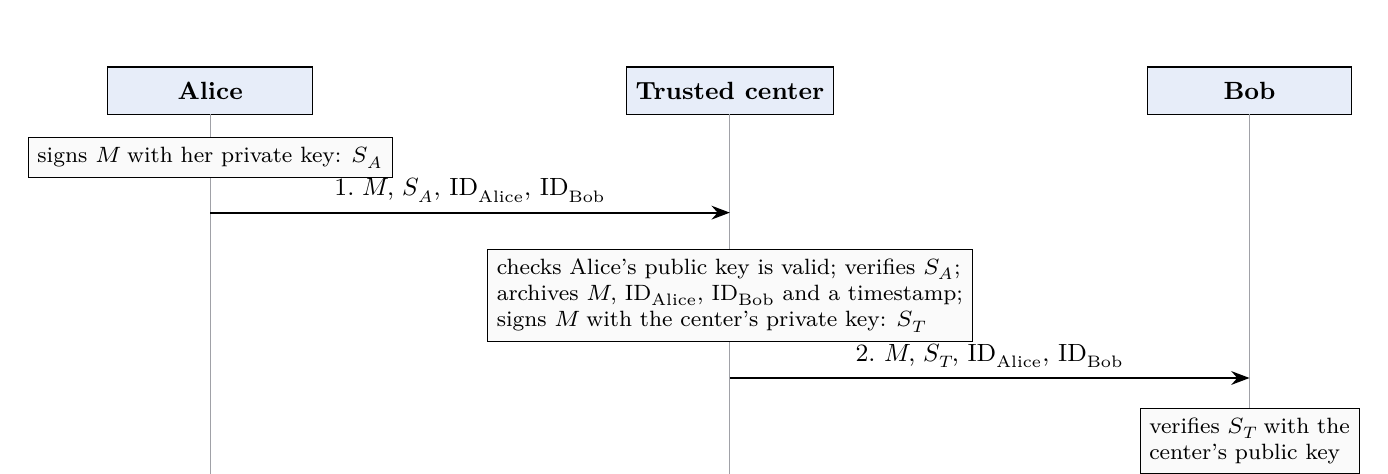
\begin{tikzpicture}[font=\small, >=Stealth]
\foreach \x/\n in {0/Alice, 6.6/Trusted center, 13.2/Bob} {
  \node[draw, fill=acc!10, minimum width=2.6cm, minimum height=0.6cm] at (\x,0) {\textbf{\n}};
  \draw[gray] (\x,-0.3) -- (\x,-5.0);
}
\node[draw, fill=white, font=\footnotesize, align=left] at (0,-0.85) {signs $M$ with her private key: $S_A$};
\draw[->, thick] (0,-1.55) -- node[above]{1.\ $M$, $S_A$, ID$_{\text{Alice}}$, ID$_{\text{Bob}}$} (6.6,-1.55);
\node[draw, fill=white, font=\footnotesize, align=left] at (6.6,-2.6) {checks Alice's public key is valid; verifies $S_A$;\\archives $M$, ID$_{\text{Alice}}$, ID$_{\text{Bob}}$ and a timestamp;\\signs $M$ with the center's private key: $S_T$};
\draw[->, thick] (6.6,-3.65) -- node[above]{2.\ $M$, $S_T$, ID$_{\text{Alice}}$, ID$_{\text{Bob}}$} (13.2,-3.65);
\node[draw, fill=white, font=\footnotesize, align=left] at (13.2,-4.45) {verifies $S_T$ with the\\center's public key};
\end{tikzpicture}
\end{center}
\begin{enumerate}[leftmargin=1.6em]
  \item Alice creates a signature $S_A$ from her message with her private key and sends the message, her identity, Bob's identity and $S_A$ to the center. The identities bind the message to this particular sender and recipient.
  \item The center, after checking that Alice's public key is valid, verifies through it that the message came from Alice. Checking validity at this moment is what defeats a later ``I had changed my key'' claim.
  \item The center saves a copy of the message with the sender identity, the recipient identity and a \textbf{timestamp} in its archive. The archive is the independent evidence; the timestamp also distinguishes this message from a later replay of it.
  \item The center uses its own private key to create another signature $S_T$ from the message, and sends the message, $S_T$, Alice's identity and Bob's identity to Bob.
  \item Bob verifies the message using the public key of the trusted center.
\end{enumerate}
If Alice later denies the message, the center shows the archived copy, which it accepted only after verifying Alice's signature with her then-valid key; Alice cannot deny it, and Bob's copy carries the center's signature, so he cannot have invented it either. \imp{Nonrepudiation can be provided using a trusted party.}

\textbf{No confidentiality.} A digital signature does not provide privacy: the message travels in clear (and in RSA anyone can even compute $M = S^e$ from the signature), since the goal is not to hide the message but to prove who sent it. If confidentiality is required, the message and the signature must be encrypted with a secret-key or public-key cryptosystem, adding another layer of encryption and decryption. Alice first signs with her private key, then encrypts $(M, S)$ with Bob's public key (or a shared session key); Bob decrypts with his private key and then verifies with Alice's public key.
\begin{center}
\begin{tikzpicture}[font=\small, >=Stealth]
\node (m) at (0,0) {$M$};
\node[dsgop, fill=acc!10] (sg) at (1.7,0) {Signing};
\node[dsgop, fill=warn!10] (en) at (4.6,0) {Encryption};
\node[dsgop, fill=warn!10] (de) at (9.6,0) {Decryption};
\node[dsgop, fill=acc!10] (vf) at (12.5,0) {Verifying};
\node (out) at (14.4,0) {$M$};
\node[font=\footnotesize, align=center] at (1.7,0.95) {Alice's\\private key};
\node[font=\footnotesize, align=center] at (4.6,0.95) {Bob's\\public key};
\node[font=\footnotesize, align=center] at (9.6,0.95) {Bob's\\private key};
\node[font=\footnotesize, align=center] at (12.5,0.95) {Alice's\\public key};
\foreach \n in {sg, en, de, vf} \draw[->] (\n.north) ++(0,0.25) -- (\n.north);
\draw[->] (m) -- (sg); \draw[->] (sg) -- node[above, font=\footnotesize]{$(M, S)$} (en);
\draw[->] (en) -- node[above]{encrypted $(M, S)$} node[below, font=\footnotesize]{insecure channel} (de);
\draw[->] (de) -- node[above, font=\footnotesize]{$(M, S)$} (vf); \draw[->] (vf) -- (out);
\draw[decorate, decoration={brace, mirror, amplitude=4pt}] (0.8,-0.45) -- node[below=4pt, font=\footnotesize]{Alice} (5.6,-0.45);
\draw[decorate, decoration={brace, mirror, amplitude=4pt}] (8.6,-0.45) -- node[below=4pt, font=\footnotesize]{Bob} (13.4,-0.45);
\end{tikzpicture}
\end{center}
The order \textbf{sign, then encrypt} matters. The signature is then on the plaintext, so Bob can later show $(M, S)$ to a judge without revealing his private key. If Alice encrypted first and signed the ciphertext, Eve could strip Alice's signature and attach her own to the same ciphertext, claiming authorship of a message she cannot even read.

\subsection{Attacks on digital signatures; types of forgery \new}
\likely{``Explain key-only, known-message and chosen-message attacks; differentiate existential and selective forgery'' (3--4 marks).}

Attacks are classified by what Eve has access to, exactly as attacks on ciphers were.
\begin{itemize}[leftmargin=1.4em]
  \item \textbf{Key-only attack.} Eve has access only to the public information released by Alice (her public key). To forge a message, she must create Alice's signature to convince Bob that the message comes from Alice. This is the analogue of the ciphertext-only attack on encipherment.
  \item \textbf{Known-message attack.} Eve has access to one or more message--signature pairs, i.e.\ some documents previously signed by Alice, and tries to create another message and forge Alice's signature on it. This is the analogue of the known-plaintext attack.
  \item \textbf{Chosen-message attack.} Eve somehow makes Alice sign one or more messages of Eve's choice, so she holds chosen-message/signature pairs. She later creates another message, with the content she wants, and forges Alice's signature on it. This is the analogue of the chosen-plaintext attack, and the strongest of the three.
\end{itemize}
If an attack succeeds, the result is a \textbf{forgery}, of one of two types.

\textbf{Existential forgery.} Eve is able to create a valid message--signature pair, but not one she can really use: the document is forged, but its content is calculated by the algebra (effectively random), so the message is likely to be syntactically or semantically unintelligible. Such forgery is probable for unprotected schemes, but Eve cannot benefit from it very much.

\textbf{Selective forgery.} Eve is able to forge Alice's signature on a message whose content \emph{Eve selected}. This is beneficial to Eve and may be very detrimental to Alice; the probability of such forgery is low, but not negligible.

\begin{center}\small
\begin{tabularx}{\textwidth}{@{}l X X X@{}}
\toprule
Forgery & What Eve obtains & Who chooses the content & Likelihood and harm\\
\midrule
Existential & at least one valid $(M, S)$ & the algebra (random-looking $M$) & likely for raw (unhashed) schemes; little benefit\\
Selective & a valid $S$ on a message she chose beforehand & Eve & low probability, very harmful\\
\bottomrule
\end{tabularx}
\end{center}
Stallings adds two stronger outcomes: a \textbf{universal forgery} (Eve can sign \emph{any} message) and a \textbf{total break} (Eve recovers the private key). A scheme is considered secure only if even the weakest outcome, existential forgery, is infeasible under the strongest attack, the chosen-message attack.

%%%PART3%%%

% College Lecture 16: key management (slides L16, 20 slides) + Forouzan ch. 15 (KDC, Needham-Schroeder, Otway-Rees,
% Kerberos, Diffie-Hellman, STS, public-key distribution, X.509, PKI) + Stallings (key distribution, Kerberos v4/v5,
% X.509, PKI trust). Every number recomputed by script (scratchpad/w21/verify.py).
\section{Key Management and Key Distribution}\label{sec:keymgmt}
\usetikzlibrary{decorations.pathreplacing}
\tikzset{
  kmact/.style={draw, rounded corners=2pt, fill=acc!10, font=\small\bfseries, minimum width=1.5cm, minimum height=0.6cm, inner sep=2pt},
  kmn/.style={circle, fill=black, text=white, font=\scriptsize\bfseries, inner sep=0pt, minimum size=3.8mm},
  kmdo/.style={draw, fill=gray!12, font=\footnotesize, inner sep=2pt, align=center},
  kmm/.style={-{Stealth[length=2mm]}, thick},
  kmu/.style={circle, draw, fill=acc!10, minimum size=6mm, inner sep=0pt, font=\footnotesize},
  kmca/.style={draw, rounded corners=2pt, fill=gold!15, font=\footnotesize, inner sep=2pt, minimum height=5mm}
}
% \kmLife{x}{name}{bottom y}: actor box and lifeline.  \kmMsg{y}{from x}{to x}{number}{label}: numbered message arrow.
\providecommand{\kmLife}[3]{\node[kmact] at (#1,0) {#2}; \draw[gray!80] (#1,-0.32) -- (#1,#3);}
\providecommand{\kmMsg}[5]{\node[kmn] (kmN) at (#2,#1) {#4}; \draw[kmm] (kmN) -- node[above, font=\footnotesize, inner sep=1.5pt, align=center, fill=white]{#5} (#3,#1);}
\providecommand{\kmK}[1]{K_{\text{#1}}}

\textbf{Notation.} $E_K(X)$ is $X$ encrypted with the symmetric key $K$; a comma inside $E_K(\cdot)$ means concatenation. $K_A$ is Alice's long-term \emph{master key} shared with the key-distribution center, $K_{AB}$ a \emph{session key} between Alice and Bob, $R_A$ a \emph{nonce} (a random number used only once) chosen by Alice, and $T$ a timestamp. In the diagrams a black circle marks the sender and the number of each message.

\subsection{The symmetric-key distribution problem: the $N^2$ problem \new}
\likely{``What is the $N^2$ problem? How many keys do $N$ users need, with and without a KDC?'' (2--3 marks).}

Symmetric-key cryptography is far faster than public-key cryptography, so it is used for all bulk data. Its weakness is that both parties must already hold the same secret key. If Alice wants to exchange confidential messages with $N$ people, she needs $N$ different keys, one per correspondent, since a key shared with Carol must not let Carol read Alice's traffic with Bob.

\textbf{Counting the keys.} Now let $N$ people all communicate with each other. Each person needs a key with each of the other $N - 1$ people, which gives $N(N-1)$ (person, partner) combinations. Every key, however, is shared by exactly two people and has therefore been counted twice, so
\[
\text{number of keys} = \frac{N(N-1)}{2} = \binom{N}{2} \quad\text{(one key per pair)}, \qquad N(N-1) \quad\text{(a separate key for each direction)}.
\]
Each person stores $N - 1$ keys. Both counts grow like $N^2$, so this is called the \textbf{$N^2$ problem}. For one million people, each person holds $999\,999$ keys and the total is $10^6(10^6 - 1)/2 = 499\,999\,500\,000 \approx 5 \times 10^{11}$ keys, or about $10^{12}$ (one trillion) if each direction has its own key. A newcomer needs $N$ new keys, all delivered securely.

\textbf{The distribution problem.} The number of keys is not the only problem: each key must reach both parties over a secure channel \emph{before} any secure communication is possible, and the Internet is not one. Stallings lists four ways for Alice and Bob to obtain a key: (1) Alice chooses it and delivers it physically to Bob; (2) a third party chooses it and delivers it physically to both; (3) if they already share a key, one sends the new key encrypted under the old one; (4) if each has an encrypted link to a trusted third party, the third party sends the key to both over those links. Physical delivery does not scale to millions of users, and option 3 still needs a first key, and one compromised key then exposes every later one. Option 4 is the key-distribution center.

\begin{center}
\begin{tikzpicture}[font=\footnotesize]
\foreach \n [count=\i] in {A,B,C,D,E} \node[kmu] (m\n) at ({90+72*(\i-1)}:1.75) {\n};
\foreach \a/\b in {A/B,A/C,A/D,A/E,B/C,B/D,B/E,C/D,C/E,D/E} \draw[gray] (m\a) -- (m\b);
\node at (0,-2.3) {without a KDC: $\binom{5}{2} = 10$ pairwise keys};
\begin{scope}[xshift=7cm]
\node[kmca] (kdc) at (0,0) {KDC};
\foreach \n [count=\i] in {A,B,C,D,E} {\node[kmu] (k\n) at ({90+72*(\i-1)}:1.9) {\n};
  \draw[dashed] (k\n) -- node[font=\scriptsize, fill=white, inner sep=0.5pt, pos=0.45]{$K_{\n}$} (kdc);}
\node at (0,-2.3) {with a KDC: $5$ master keys};
\end{scope}
\end{tikzpicture}
\end{center}
\begin{center}\small
\begin{tabular}{@{}rrrr@{}}
\toprule
Users $N$ & Keys per user & Pairwise keys $N(N-1)/2$ & Keys with a KDC ($N$)\\
\midrule
10 & 9 & 45 & 10\\
100 & 99 & 4\,950 & 100\\
1\,000 & 999 & 499\,500 & 1\,000\\
$10^6$ & 999\,999 & $\approx 5 \times 10^{11}$ & $10^6$\\
\bottomrule
\end{tabular}
\end{center}

\subsection{Key-distribution center (KDC) and session keys \new}
\likely{``Explain the role of a KDC; why are session keys temporary; flat versus hierarchical KDCs'' (3--4 marks).}

A practical solution is a trusted third party called a \textbf{key-distribution center (KDC)}. \imp{Each member establishes one secret key, the master key, with the KDC}: Alice shares $K_{\text{Alice}}$ (written $K_A$), Bob shares $K_B$, and so on. The master key is set up once, for example in person when the member registers, and is used only between the member and the KDC, never between two members. As a result $N$ members need only $N$ master keys, and a newcomer needs one key instead of $N$.

\textbf{Session keys.} When Alice wants to talk to Bob, she asks the KDC for a \textbf{session key} $K_{AB}$, a fresh random key valid only for one conversation. The KDC uses the master keys to deliver $K_{AB}$ secretly to both and to authenticate Alice and Bob to the center and to each other. When the conversation ends the session key is discarded. Session keys are kept temporary for four reasons. First, the less ciphertext is produced under one key, the less material a cryptanalyst has. Second, a compromised session key exposes only one session. Third, the master key is then used only to encrypt short random session keys, so it is rarely exposed and can stay valid for a long time. Fourth, the KDC need not store $N(N-1)/2$ pairwise keys, because it creates each one on demand. This two-level arrangement (long-term master keys protecting short-term session keys) is the \textbf{key hierarchy}.

The slides describe the flow conceptually: Alice requests a session key with Bob, the KDC informs Bob, and if Bob agrees a session key is created. In the actual protocols below, the KDC does not contact Bob itself; it gives Alice two copies of $K_{AB}$, one encrypted under $K_A$ and one sealed under $K_B$ in a \textbf{ticket}, and Alice forwards the ticket to Bob.

\textbf{Multiple KDCs.} A single KDC for the whole world would be a bottleneck and a single point of failure, and everyone would have to register with it. In \textbf{flat multiple KDCs} the world is divided into domains, each with one or more KDCs (more than one for redundancy). If Alice and Bob are in different domains, Alice contacts her KDC, which contacts the KDC of Bob's domain, and the two KDCs together create the session key. In \textbf{hierarchical multiple KDCs} the KDCs form a tree, for example local, national and international KDCs. A request from Alice to Bob in another country goes up from Alice's local KDC through her national KDC to an international KDC, and then down through Bob's national KDC to Bob's local KDC.

\begin{center}
\begin{tikzpicture}[font=\footnotesize, k/.style={kmca, minimum width=2.3cm}]
\node[k] (int) at (0,0) {International KDC};
\node[k] (n1) at (-3.6,-1.1) {National KDC (India)};
\node[k] (n2) at (3.6,-1.1) {National KDC (USA)};
\node[k] (l1) at (-5.4,-2.2) {Local KDC 1};
\node[k] (l2) at (-1.8,-2.2) {Local KDC 2};
\node[k] (l3) at (1.8,-2.2) {Local KDC 3};
\node[k] (l4) at (5.4,-2.2) {Local KDC 4};
\node[kmu] (al) at (-5.4,-3.2) {A}; \node[kmu] (bo) at (5.4,-3.2) {B};
\foreach \a/\b in {n1/l2,n2/l3} \draw[gray] (\a) -- (\b);
\foreach \a/\b in {al/l1,l1/n1,n1/int,int/n2,n2/l4,l4/bo} \draw[kmm, orange] (\a) -- (\b);
\node[font=\scriptsize, orange, align=left] at (0,-1.5) {request path\\Alice $\to$ \dots $\to$ Bob};
\end{tikzpicture}
\end{center}
\textbf{Advantages of the hierarchy.} Most master keys are shared between a local KDC and its local users, so the effort of distributing master keys stays local. A faulty or subverted KDC damages only its own subtree. The KDCs themselves need far fewer keys: $M$ KDCs in a flat full mesh need $M(M-1)/2$ inter-KDC keys, but a tree of $M$ KDCs has only $M - 1$ edges. \textbf{Disadvantage of every KDC scheme.} The KDC knows every session key, so it must be completely trusted, and it must be online for every new session.

\subsection{Session-key creation: a simple KDC protocol and its flaw \new}
\likely{``Show the simple KDC protocol; why is it vulnerable to replay?'' (2--3 marks).}

The simplest protocol uses three messages.
\begin{center}
\begin{tikzpicture}[font=\footnotesize]
\kmLife{0}{Alice}{-3.3} \kmLife{6.5}{KDC}{-3.3} \kmLife{13}{Bob}{-3.3}
\kmMsg{-0.9}{0}{6.5}{1}{Alice, Bob \ (plaintext)}
\kmMsg{-1.8}{6.5}{0}{2}{$E_{K_A}\bigl(K_{AB},\ \text{Ticket}\bigr)$, \ Ticket $= E_{K_B}(\text{Alice}, \text{Bob}, K_{AB})$}
\kmMsg{-2.7}{0}{13}{3}{Ticket $= E_{K_B}(\text{Alice}, \text{Bob}, K_{AB})$}
\end{tikzpicture}
\end{center}
\begin{enumerate}
  \item Alice sends the KDC a plaintext request containing her registered identity and Bob's identity. Nothing in it is secret.
  \item The KDC creates $K_{AB}$ and a \textbf{ticket} for Bob, encrypted with $K_B$ and containing both identities and $K_{AB}$. It sends Alice the ticket together with a copy of $K_{AB}$, the whole message encrypted with $K_A$ (the ticket is therefore encrypted twice). Only Alice can open the message and extract $K_{AB}$; she cannot read the ticket, because it is meant for Bob.
  \item Alice forwards the ticket to Bob. Only Bob can open it, and since only the KDC could have made it, Bob learns that Alice wants to talk to him using $K_{AB}$. Alice trusts the KDC, so she is assured that only Bob can recover the key; Bob trusts the KDC, so he is assured that the key belongs to a session with Alice.
\end{enumerate}
\textbf{The flaw: no freshness.} Nothing in the messages shows that they are new. Eve can record message 3 and the session that follows, and later \textbf{replay} them; Bob accepts the old ticket and acts on the old messages a second time (for example, a repeated money transfer). Worse, if Eve ever breaks an old session key, she can answer a new request of Alice by replaying the old message 2, and Alice will use a key Eve knows. There is a third weakness: message 1 is not protected, so Eve can replace ``Bob'' by ``Eve''; the KDC then returns a ticket under $K_{\text{Eve}}$, Alice's part does not name the partner, and Alice unknowingly shares $K_{AB}$ with Eve. The next protocol closes all three holes.

\subsection{The Needham--Schroeder protocol \new}
\likely{``Draw and explain the Needham--Schroeder protocol; what is the purpose of each nonce; describe the Denning--Sacco attack'' (5 marks).}

Needham and Schroeder (1978) designed the protocol that is the foundation of many later ones, including Kerberos. It uses challenge--response with two nonces, $R_A$ (Alice's challenge to the KDC) and $R_B$ (Bob's challenge to Alice).
\begin{center}
\begin{tikzpicture}[font=\footnotesize]
\kmLife{0}{Alice}{-5.0} \kmLife{6.5}{KDC}{-5.0} \kmLife{13}{Bob}{-5.0}
\kmMsg{-0.9}{0}{6.5}{1}{$R_A$, Alice, Bob}
\kmMsg{-1.8}{6.5}{0}{2}{$E_{K_A}\bigl(R_A,\ \text{Bob},\ K_{AB},\ \text{Ticket}\bigr)$}
\node[font=\scriptsize, gray!50!black] at (3.25,-2.15) {Ticket $= E_{K_B}(\text{Alice}, K_{AB})$};
\kmMsg{-2.9}{0}{13}{3}{Ticket $= E_{K_B}(\text{Alice}, K_{AB})$}
\kmMsg{-3.7}{13}{0}{4}{$E_{K_{AB}}(R_B)$}
\kmMsg{-4.5}{0}{13}{5}{$E_{K_{AB}}(R_B - 1)$}
\end{tikzpicture}
\end{center}
\begin{enumerate}
  \item \textbf{Alice $\to$ KDC: $R_A$, Alice, Bob.} The nonce $R_A$ is a fresh challenge to the KDC. The message may travel in plaintext.
  \item \textbf{KDC $\to$ Alice: $E_{K_A}(R_A, \text{Bob}, K_{AB}, \text{Ticket})$.} Returning $R_A$ proves to Alice that this reply was made for \emph{this} request, so an old message 2 (perhaps carrying a broken key) cannot be replayed. Including ``Bob'' lets Alice check that the key is for the partner she asked for, which defeats the substitution of ``Eve'' in message 1. The whole message is encrypted with $K_A$, so only Alice learns $K_{AB}$, and the fields cannot be cut apart and recombined. The ticket $E_{K_B}(\text{Alice}, K_{AB})$ gives Bob the key and tells him with whom he shares it.
  \item \textbf{Alice $\to$ Bob: the ticket.} Bob decrypts it with $K_B$ and obtains $K_{AB}$ and Alice's identity.
  \item \textbf{Bob $\to$ Alice: $E_{K_{AB}}(R_B)$.} Bob challenges the sender to prove that it holds $K_{AB}$ now. A replayed ticket from someone who does not know $K_{AB}$ fails here.
  \item \textbf{Alice $\to$ Bob: $E_{K_{AB}}(R_B - 1)$.} Alice decrypts $R_B$, subtracts 1 and re-encrypts. The transformation is essential: if Alice simply returned $E_{K_{AB}}(R_B)$, Eve could reflect message 4 back to Bob without knowing the key. Only a holder of $K_{AB}$ can produce $E_{K_{AB}}(R_B - 1)$.
\end{enumerate}

\textbf{The Denning--Sacco replay attack (1981).} Alice receives a freshness guarantee through $R_A$, but Bob receives none: the ticket contains nothing chosen by Bob and no time. Suppose Eve recorded message 3 of an old session and has since learned that session's key $K_{AB}$ (by cryptanalysis of the old traffic, or because the key was carelessly disposed of). She replays the old ticket to Bob, decrypts his challenge with the known key, and answers it:
\begin{center}
\begin{tikzpicture}[font=\footnotesize]
\kmLife{0}{Eve (as Alice)}{-3.3} \kmLife{8}{Bob}{-3.3}
\kmMsg{-0.9}{0}{8}{3}{old Ticket $= E_{K_B}(\text{Alice}, K_{AB})$}
\kmMsg{-1.8}{8}{0}{4}{$E_{K_{AB}}(R_B')$}
\kmMsg{-2.7}{0}{8}{5}{$E_{K_{AB}}(R_B' - 1)$ \ (Eve knows $K_{AB}$)}
\end{tikzpicture}
\end{center}
Bob now believes he shares a fresh key with Alice, and Eve can impersonate Alice for as long as she likes. The challenge $R_B$ does not help, because Eve really does know the (old) key. Two fixes exist.
\begin{itemize}
  \item \textbf{Timestamps (Denning--Sacco).} The KDC puts a timestamp $T$ in message 2 and in the ticket, $E_{K_B}(\text{Alice}, K_{AB}, T)$. Bob accepts only if $|\text{Clock} - T| < \Delta t_1 + \Delta t_2$, where $\Delta t_1$ is the expected difference between the KDC's clock and his own and $\Delta t_2$ the expected network delay. An old ticket fails this test. The price is that all clocks must be synchronised; this is the route Kerberos takes.
  \item \textbf{Bob's nonce inside the ticket (revised protocol, 1987).} Bob first gives Alice a nonce sealed under his own key, and the KDC copies it into the ticket, so Bob can see that the ticket was issued after his nonce. This gives the seven-message version below.
\end{itemize}
\begin{center}
\begin{tikzpicture}[font=\footnotesize]
\kmLife{0}{Alice}{-6.6} \kmLife{6.5}{KDC}{-6.6} \kmLife{13}{Bob}{-6.6}
\kmMsg{-0.9}{0}{13}{1}{Alice}
\kmMsg{-1.7}{13}{0}{2}{$E_{K_B}(\text{Alice}, R_B')$}
\kmMsg{-2.5}{0}{6.5}{3}{$R_A$, Alice, Bob, $E_{K_B}(\text{Alice}, R_B')$}
\kmMsg{-3.3}{6.5}{0}{4}{$E_{K_A}\bigl(R_A, \text{Bob}, K_{AB}, \text{Ticket}\bigr)$}
\kmMsg{-4.3}{0}{13}{5}{Ticket $= E_{K_B}(\text{Alice}, K_{AB}, R_B')$}
\kmMsg{-5.2}{13}{0}{6}{$E_{K_{AB}}(R_B)$}
\kmMsg{-6.1}{0}{13}{7}{$E_{K_{AB}}(R_B - 1)$}
\end{tikzpicture}
\end{center}
In messages 1--2 Bob issues the nonce $R_B'$, sealed so that Alice can neither read nor change it. Alice passes it to the KDC in message 3, the KDC places it inside Bob's ticket in message 4, and in message 5 Bob checks that the ticket contains the nonce he issued in this run. An old ticket carries an old nonce and is rejected. Messages 6--7 are the key confirmation of the original protocol.

\subsection{The Otway--Rees protocol \new}
\likely{``Draw the Otway--Rees protocol; what is the role of the common nonce?'' (4--5 marks).}

Otway and Rees (1987) give both parties their own freshness guarantee and let \emph{Bob}, not Alice, talk to the KDC. A \textbf{common nonce} $R$ identifies the run, and each party adds a private nonce ($R_A$, $R_B$) inside a part encrypted for the KDC.
\begin{center}
\begin{tikzpicture}[font=\footnotesize]
\kmLife{0}{Alice}{-4.9} \kmLife{6.8}{Bob}{-4.9} \kmLife{14.4}{KDC}{-4.9}
\kmMsg{-0.9}{0}{6.8}{1}{$R$, Alice, Bob, $E_{K_A}(R_A, R, \text{Alice}, \text{Bob})$}
\kmMsg{-2.0}{6.8}{14.4}{2}{$R$, Alice, Bob, $E_{K_A}(R_A, R, \text{Alice}, \text{Bob})$,\\ $E_{K_B}(R_B, R, \text{Alice}, \text{Bob})$}
\kmMsg{-2.9}{14.4}{6.8}{3}{$R$, $E_{K_A}(R_A, K_{AB})$, $E_{K_B}(R_B, K_{AB})$}
\kmMsg{-3.7}{6.8}{0}{4}{$R$, $E_{K_A}(R_A, K_{AB})$}
\kmMsg{-4.5}{0}{6.8}{5}{$E_{K_{AB}}(\text{short message})$}
\end{tikzpicture}
\end{center}
\begin{enumerate}
  \item Alice sends Bob the common nonce $R$, both identities, and a part for the KDC encrypted with $K_A$ that contains her nonce $R_A$ (her challenge to the KDC), a copy of $R$ and the identities.
  \item Bob creates the same kind of part with his own nonce $R_B$ under $K_B$, and sends both encrypted parts to the KDC. The KDC decrypts them and checks that the $R$ and the identities inside \emph{both} parts agree with the plaintext. This proves that Alice and Bob each asked for a key with the other in this very run, so Eve cannot splice requests from different runs.
  \item The KDC creates $K_{AB}$ and returns $R$ with two sealed parts, $E_{K_A}(R_A, K_{AB})$ for Alice and $E_{K_B}(R_B, K_{AB})$ for Bob. Bob opens his part and checks $R_B$: the key was made in answer to his current request.
  \item Bob forwards Alice's part. Alice checks $R_A$, so she too knows the key is fresh.
  \item (Forouzan) Alice sends a short message encrypted with $K_{AB}$ to show that she has the key (key confirmation).
\end{enumerate}
\textbf{Why this defeats the Denning--Sacco replay.} Bob obtains the key from a part that contains his own fresh $R_B$, so an old message 3 is rejected even if Eve knows the old $K_{AB}$. No synchronised clocks are needed. A known weakness is a \emph{type-flaw} attack: Eve reflects Alice's encrypted part from message 1 back to her in message 4, and if Alice cannot tell the field types apart she accepts $(R, \text{Alice}, \text{Bob})$ as the key; tagging each field with its type stops this.

\subsection{Kerberos \hot\new}\label{sec:kerberos}
\likely{``Draw and explain Kerberos: AS, TGS, server and the six messages'' (8--10 marks); ``why is the TGS separate from the AS?''; ``differentiate Kerberos v4 and v5''.}

\textbf{The problem.} In a campus or company network, users sit at workstations and use services on many servers (mail, files, printing). Each server must know who is asking, but the network is open: a user may pretend to be another, a workstation may forge its network address, and Eve may record and replay traffic. Building password checks into every server would scatter passwords everywhere and send them over the network. \textbf{Kerberos}, developed at MIT (Project Athena), is \imp{an authentication protocol and at the same time a KDC}: a central server authenticates every user once, and then hands out tickets and session keys for the other servers, so that the password is typed once per logon and never travels over the network. Version 4 is described in Forouzan and Stallings; version 5 is the standard in use (for example in Windows domains).

\textbf{The three servers.} The \textbf{authentication server (AS)} is the KDC of Kerberos: every user registers with it and it holds a key derived from each user's password. It verifies the user and issues a session key and a ticket for the TGS. The \textbf{ticket-granting server (TGS)} issues tickets for the real servers and creates the session key between the user and the server. The \textbf{real server} (Bob) provides the service. In the notation below, $\kmK{A-AS}$ is Alice's long-term key with the AS, $\kmK{AS-TGS}$ and $\kmK{TGS-B}$ are long-term keys between servers, and $\kmK{A-TGS}$, $\kmK{A-B}$ are session keys.
\begin{center}
\begin{tikzpicture}[font=\footnotesize]
\kmLife{2.4}{Alice}{-5.6} \kmLife{6.6}{AS}{-5.6} \kmLife{10.8}{TGS}{-5.6} \kmLife{15.4}{Bob}{-5.6}
\kmMsg{-0.9}{2.4}{6.6}{1}{Alice, TGS, $TS_1$}
\kmMsg{-1.7}{6.6}{2.4}{2}{$E_{\kmK{A-AS}}(\kmK{A-TGS},\ \text{TGT})$}
\kmMsg{-2.6}{2.4}{10.8}{3}{TGT, \ Bob, \ $E_{\kmK{A-TGS}}(\text{Alice}, TS_3)$}
\kmMsg{-3.4}{10.8}{2.4}{4}{$E_{\kmK{A-TGS}}(\text{Bob}, \kmK{A-B})$, \ Ticket$_B$}
\kmMsg{-4.3}{2.4}{15.4}{5}{Ticket$_B$, \ $E_{\kmK{A-B}}(\text{Alice}, TS_5)$}
\kmMsg{-5.1}{15.4}{2.4}{6}{$E_{\kmK{A-B}}(TS_5 + 1)$}
\draw[decorate, decoration={brace, amplitude=3pt, mirror}] (1.55,-0.7) -- node[left=3pt, align=right, font=\scriptsize]{once per\\logon} (1.55,-1.9);
\draw[decorate, decoration={brace, amplitude=3pt, mirror}] (1.55,-2.4) -- node[left=3pt, align=right, font=\scriptsize]{once per\\server} (1.55,-3.6);
\draw[decorate, decoration={brace, amplitude=3pt, mirror}] (1.55,-4.1) -- node[left=3pt, align=right, font=\scriptsize]{once per\\session} (1.55,-5.3);
\end{tikzpicture}

\small TGT $= E_{\kmK{AS-TGS}}(\text{Alice}, \kmK{A-TGS}, \dots)$ \qquad Ticket$_B = E_{\kmK{TGS-B}}(\text{Alice}, \kmK{A-B}, \dots)$
\end{center}
\begin{enumerate}
  \item \textbf{Alice $\to$ AS.} Alice sends her request in plaintext, using her registered identity.
  \item \textbf{AS $\to$ Alice.} The AS replies with a message encrypted with Alice's permanent key $\kmK{A-AS}$. It contains the session key $\kmK{A-TGS}$ for talking to the TGS and a \textbf{ticket-granting ticket (TGT)} encrypted with the TGS's key $\kmK{AS-TGS}$. Alice does not store $\kmK{A-AS}$: when the message arrives she types her password, and the password with a fixed algorithm (a one-way function) produces $\kmK{A-AS}$ if the password is correct. The password and $\kmK{A-AS}$ are used for this one decryption and then destroyed; the password is never sent over the network and does not stay in the workstation.
  \item \textbf{Alice $\to$ TGS.} Alice sends three items: the TGT, the name of the real server (Bob), and a timestamp encrypted with $\kmK{A-TGS}$ (the \textbf{authenticator}). The TGS opens the TGT with $\kmK{AS-TGS}$, takes $\kmK{A-TGS}$ from it, and checks the authenticator. The timestamp prevents a replay by Eve, who cannot make a new one without $\kmK{A-TGS}$.
  \item \textbf{TGS $\to$ Alice.} The TGS sends two tickets, each containing the new session key $\kmK{A-B}$: Alice's copy is encrypted with $\kmK{A-TGS}$, Bob's copy (Ticket$_B$) with Bob's key $\kmK{TGS-B}$. Eve cannot extract $\kmK{A-B}$, since she knows neither key. Even if she replays message 3 before its timestamp expires, she only receives the same two tickets, which she cannot decrypt.
  \item \textbf{Alice $\to$ Bob.} Alice sends Bob's ticket with a timestamp encrypted under $\kmK{A-B}$.
  \item \textbf{Bob $\to$ Alice.} Bob confirms receipt by adding 1 to the timestamp, encrypted with $\kmK{A-B}$. Only the real Bob could open the ticket and read the timestamp, so Alice now knows she is talking to Bob (mutual authentication).
\end{enumerate}
To use another server (say a printer), Alice repeats only messages 3--6 with the same TGT; messages 1--2 are needed once per logon.

\textbf{Every field of version 4 (Stallings).} The diagram shows the core; the full messages carry identities, addresses and lifetimes, each with a job. $\text{AD}_A$ is the network address of Alice's workstation, and an authenticator $\text{Auth}$ is $E_{\text{session key}}(\text{Alice}, \text{AD}_A, TS)$.
\begin{center}\small
\begin{tabularx}{\textwidth}{@{}l>{\raggedright\arraybackslash}p{6.2cm}X@{}}
\toprule
Msg & Contents & Why each field is there\\
\midrule
(1) & Alice, TGS, $TS_1$ & Asks for a TGT; $TS_1$ lets the AS check that Alice's clock is synchronised.\\
(2) & $E_{\kmK{A-AS}}(\kmK{A-TGS}$, TGS, $TS_2$, Lifetime$_2$, TGT$)$ & Only the holder of the password can read it. $\kmK{A-TGS}$ is Alice's copy of the session key; ``TGS'' confirms whom the ticket is for; $TS_2$ and Lifetime$_2$ tell her when it expires.\\
 & TGT $= E_{\kmK{AS-TGS}}(\kmK{A-TGS}$, Alice, $\text{AD}_A$, TGS, $TS_2$, Lifetime$_2)$ & Readable only by the TGS, so Alice cannot alter it. ``Alice'' names the owner, $\text{AD}_A$ ties the ticket to her workstation, and the lifetime bounds how long a stolen ticket is useful.\\
(3) & Bob, TGT, $\text{Auth} = E_{\kmK{A-TGS}}(\text{Alice}, \text{AD}_A, TS_3)$ & A TGT can be copied off the network; the authenticator proves that the sender knows $\kmK{A-TGS}$ \emph{now}. The TGS checks that the name and address match the TGT and that $TS_3$ is current.\\
(4) & $E_{\kmK{A-TGS}}(\kmK{A-B}$, Bob, $TS_4$, Ticket$_B)$ & Encrypted with the session key, so no password is needed for further servers. ``Bob'' and $TS_4$ confirm the server and the issue time.\\
 & Ticket$_B = E_{\kmK{TGS-B}}(\kmK{A-B}$, Alice, $\text{AD}_A$, Bob, $TS_4$, Lifetime$_4)$ & Readable only by Bob; reusable for repeated access to Bob until it expires.\\
(5) & Ticket$_B$, $\text{Auth} = E_{\kmK{A-B}}(\text{Alice}, \text{AD}_A, TS_5)$ & Bob opens the ticket with $\kmK{TGS-B}$, obtains $\kmK{A-B}$, and checks the fresh authenticator.\\
(6) & $E_{\kmK{A-B}}(TS_5 + 1)$ & Proves Bob's identity (only he could read $TS_5$); the $+1$ makes it differ from anything Alice sent, so it cannot be reflected.\\
\bottomrule
\end{tabularx}
\end{center}

\textbf{What each key protects.}
\begin{center}\small
\begin{tabular}{@{}llll@{}}
\toprule
Key & Shared by & Origin and lifetime & Protects\\
\midrule
$\kmK{A-AS}$ & Alice, AS & long-term, derived from Alice's password & message 2\\
$\kmK{AS-TGS}$ & AS, TGS & long-term, set by the administrator & the TGT\\
$\kmK{A-TGS}$ & Alice, TGS & session key made by the AS, lives as long as the TGT & authenticator of 3, message 4\\
$\kmK{TGS-B}$ & TGS, Bob & long-term, set by the administrator & Ticket$_B$\\
$\kmK{A-B}$ & Alice, Bob & session key made by the TGS & authenticator of 5, message 6, data\\
\bottomrule
\end{tabular}
\end{center}

\textbf{Tickets versus authenticators.} A \textbf{ticket} is made by a Kerberos server, encrypted with the key of the server it is meant for, and can be reused until its lifetime ends. An \textbf{authenticator} is made by the client, encrypted with the session key from the ticket, has a very short lifetime and is used once. The ticket delivers the session key securely; the authenticator proves that the person presenting the ticket is its owner, since a ticket alone could have been copied from the network.

\textbf{Why the TGS is separate from the AS.} Alice contacts several servers in one day. If the AS issued server tickets directly, every reply would be encrypted with the password-derived key $\kmK{A-AS}$, so Alice would have to type her password for every new server, or the workstation would have to keep $\kmK{A-AS}$ in memory all day, exposing the long-term key. Splitting the roles solves this: \imp{Kerberos separates user verification (AS, once per logon) from ticket issuing (TGS, once per server)}. The password is typed once, $\kmK{A-AS}$ is used once and destroyed, and all later requests use the TGT and the session key $\kmK{A-TGS}$, which expires with the TGT. This is \textbf{single sign-on}. A stolen $\kmK{A-TGS}$ is useful only until the TGT expires, while the password itself is never exposed again.

\textbf{Realms and inter-realm authentication.} A \textbf{realm} is one Kerberos server (AS and TGS) together with the users and application servers registered with it: the server holds every user's password-derived key and shares a secret key with every application server. Organisations with separate administrations run separate realms. For Alice in realm A to use Bob in realm B, the Kerberos servers of the two realms must share a secret key, which makes the TGS of realm B a ``server'' that the TGS of realm A can issue tickets for.
\begin{center}
\begin{tikzpicture}[font=\footnotesize]
\kmLife{0}{Alice (realm A)}{-6.3} \kmLife{5}{AS + TGS (realm A)}{-6.3} \kmLife{10}{TGS (realm B)}{-6.3} \kmLife{14.6}{Bob (realm B)}{-6.3}
\kmMsg{-0.9}{0}{5}{1}{request TGT}
\kmMsg{-1.6}{5}{0}{2}{TGT (for local TGS)}
\kmMsg{-2.4}{0}{5}{3}{request ticket for remote TGS}
\kmMsg{-3.1}{5}{0}{4}{ticket for TGS of realm B}
\kmMsg{-3.9}{0}{10}{5}{request ticket for Bob (with that ticket)}
\kmMsg{-4.6}{10}{0}{6}{Ticket$_B$}
\kmMsg{-5.6}{0}{14.6}{7}{Ticket$_B$ + authenticator: request service}
\end{tikzpicture}
\end{center}
In version 4, $N$ realms that all trust each other need $N(N-1)/2$ inter-realm keys (45 for 10 realms), the $N^2$ problem again at the level of realms; version 5 allows a hierarchy of realms with fewer keys.

\textbf{Kerberos version 4 versus version 5.} Version 5 (RFC 4120) removes environmental limits and technical flaws of version 4.
\begin{center}\small
\begin{tabularx}{\textwidth}{@{}l>{\raggedright\arraybackslash}X>{\raggedright\arraybackslash}X@{}}
\toprule
Aspect & Version 4 & Version 5\\
\midrule
Encryption & DES only & any algorithm; ciphertext tagged with type and key length\\
Network addresses & IP addresses only & any type, tagged with type and length\\
Message encoding & sender's byte order, with a flag & ASN.1 with Basic Encoding Rules (unambiguous)\\
Ticket lifetime & 8-bit field in units of 5 min, about 21 h maximum & explicit start and end times; tickets can be renewed\\
Forwarding credentials & not allowed & allowed (a server can act for the client)\\
Inter-realm & $N(N-1)/2$ realm-to-realm keys & hierarchy of realms, fewer keys\\
Double encryption & tickets encrypted a second time in messages 2 and 4 & removed\\
Mode of encryption & PCBC (non-standard, weak) & CBC with an explicit integrity check\\
Password guessing & anyone can request message 2 & pre-authentication (encrypted timestamp first)\\
Overhead & smaller & larger\\
\bottomrule
\end{tabularx}
\end{center}

\textbf{Weaknesses of Kerberos.}
\begin{itemize}
  \item \textbf{Clock synchronisation.} Freshness rests on timestamps, so all clocks must agree within a few minutes. Within that window a captured authenticator can be replayed unless servers keep a cache of recently seen authenticators, and an attacker who can change a server's clock can make old tickets look valid.
  \item \textbf{Password guessing.} Message 2 is encrypted with a key derived from the password. In version 4 anyone can ask the AS for Alice's message 2 and then try dictionary words offline: a guess is right when the decryption gives meaningful fields (the name of the TGS). Version 5 pre-authentication stops the free requests, but an eavesdropped exchange can still be attacked offline, so strong passwords remain essential.
  \item \textbf{Single point of failure and attack.} The Kerberos server holds every user's key. If it is down, nobody can log in; if it is compromised, every key is exposed. It is therefore replicated and physically protected.
  \item \textbf{Workstation compromise.} Tickets and session keys are cached on the workstation; malware there can steal a TGT and use it until it expires.
\end{itemize}

\begin{mustknow}[: Kerberos in six messages]
(1) A $\to$ AS: Alice, TGS. \ (2) AS $\to$ A: $E_{\kmK{A-AS}}(\kmK{A-TGS}, \text{TGT})$. \ (3) A $\to$ TGS: TGT, Bob, $E_{\kmK{A-TGS}}(T)$. \ (4) TGS $\to$ A: $E_{\kmK{A-TGS}}(\text{Bob}, \kmK{A-B})$, $E_{\kmK{TGS-B}}(\text{Alice}, \kmK{A-B})$. \ (5) A $\to$ B: $E_{\kmK{TGS-B}}(\text{Alice}, \kmK{A-B})$, $E_{\kmK{A-B}}(T)$. \ (6) B $\to$ A: $E_{\kmK{A-B}}(T + 1)$.\\
AS verifies the user once (password $\to \kmK{A-AS}$), TGS issues server tickets (single sign-on), timestamps stop replays.
\end{mustknow}

\subsection{Comparing the KDC-based protocols \new}
\likely{``Compare Needham--Schroeder, Otway--Rees and Kerberos'' (3 marks).}
\begin{center}\small
\begin{tabularx}{\textwidth}{@{}l>{\raggedright\arraybackslash}X>{\raggedright\arraybackslash}X>{\raggedright\arraybackslash}X@{}}
\toprule
 & Needham--Schroeder & Otway--Rees & Kerberos (v4)\\
\midrule
Messages & 5 (7 in the revised version) & 4 (+1 key confirmation) & 6 (2 once per logon)\\
Who talks to the KDC & Alice & Bob, carrying both requests & Alice (AS, then TGS)\\
Freshness by & nonces $R_A$, $R_B$ & nonces $R_A$, $R_B$ and common nonce $R$ & timestamps and lifetimes\\
Replay of an old ticket & possible (Denning--Sacco) & prevented by $R_B$ & prevented by timestamp\\
Synchronised clocks & not needed & not needed & needed\\
Proof of Bob's identity & message 4 (only Bob can read the ticket) & implicit (only Alice confirms the key) & explicit, message 6\\
Single sign-on & no & no & yes, through the TGS\\
\bottomrule
\end{tabularx}
\end{center}

\subsection{Symmetric-key agreement: Diffie--Hellman \hot\new}
\likely{``Explain Diffie--Hellman key exchange; prove that both parties get the same key; compute $R_1$, $R_2$, $K$ for given $p$, $g$, $x$, $y$'' (5--6 marks).}

A KDC needs a trusted third party that is online for every session and a master key registered in advance. In \textbf{symmetric-key agreement}, Alice and Bob create a session key between themselves, over a public channel, without a KDC and without any earlier shared secret. The slides discuss two methods: Diffie--Hellman and station-to-station.

\textbf{The idea.} Diffie and Hellman (1976) combined two facts. Modular exponentiation is a one-way function: $g^x \bmod p$ is fast to compute (square-and-multiply, \S\ref{sec:modexp}), but recovering $x$ from it is the discrete logarithm problem (\S\ref{sec:primes}), infeasible for a large prime. And exponents commute: $(g^x)^y = (g^y)^x = g^{xy}$. Each party therefore keeps an exponent secret, publishes $g$ raised to it, and raises the other's public value to its own secret exponent.

\textbf{Setup.} Before establishing a key, the two parties choose two numbers $p$ and $g$. $p$ is a large prime, on the order of 300 decimal digits (1024 bits; 2048 bits today). $g$ is a generator of order $p - 1$ in the group $\langle \mathbb{Z}_p^*, \times \rangle$, that is, a primitive root of $p$ (\S\ref{sec:fermat}), so that its powers run through all of $\mathbb{Z}_p^*$. Neither number needs to be secret: they can be sent over the Internet and shared by many users.
\begin{enumerate}
  \item Alice chooses a large random number $x$ with $0 < x < p - 1$ and calculates $R_1 = g^x \bmod p$.
  \item Bob chooses another large random number $y$ with $0 < y < p - 1$ and calculates $R_2 = g^y \bmod p$.
  \item Alice sends $R_1$ to Bob. She does not send $x$.
  \item Bob sends $R_2$ to Alice. He does not send $y$.
  \item Alice calculates $K = (R_2)^x \bmod p$.
  \item Bob calculates $K = (R_1)^y \bmod p$.
\end{enumerate}
\begin{center}
\begin{tikzpicture}[font=\footnotesize]
\kmLife{0}{Alice}{-3.9} \kmLife{9}{Bob}{-3.9}
\node[kmdo] at (0,-0.8) {$x$ secret\\$R_1 = g^x \bmod p$};
\node[kmdo] at (9,-0.8) {$y$ secret\\$R_2 = g^y \bmod p$};
\node[draw, dashed, font=\scriptsize] at (4.5,-0.8) {$p$, $g$ public};
\kmMsg{-1.65}{0}{9}{1}{$R_1$}
\kmMsg{-2.35}{9}{0}{2}{$R_2$}
\node[kmdo] at (0,-3.1) {$K = (R_2)^x \bmod p$};
\node[kmdo] at (9,-3.1) {$K = (R_1)^y \bmod p$};
\draw[dashed, ok, thick] (0,-3.75) -- node[fill=white, font=\footnotesize, text=black]{shared secret key $K = g^{xy} \bmod p$} (9,-3.75);
\end{tikzpicture}
\end{center}

\textbf{Proof that both obtain the same key.} Reducing modulo $p$ before raising to a power does not change the result modulo $p$, because $a \equiv b \pmod p$ implies $a^k \equiv b^k \pmod p$. Hence
\begin{align*}
\text{Alice: } K &= (R_2)^x \bmod p = (g^y \bmod p)^x \bmod p = g^{yx} \bmod p,\\
\text{Bob: } K &= (R_1)^y \bmod p = (g^x \bmod p)^y \bmod p = g^{xy} \bmod p ,
\end{align*}
and $g^{yx} = g^{xy}$. Both reach the same value without Bob knowing $x$ and without Alice knowing $y$: \imp{the symmetric (shared) key in the Diffie--Hellman method is $K = g^{xy} \bmod p$}.

\textbf{What Eve faces.} Eve sees $p$, $g$, $R_1 = g^x$ and $R_2 = g^y$. Computing $g^{xy}$ from these is the \textbf{(computational) Diffie--Hellman problem}; the only known general method is to solve a discrete logarithm, finding $x$ from $R_1$ (or $y$ from $R_2$), which is infeasible for a properly chosen 1024-bit or larger $p$. Note that Diffie--Hellman encrypts nothing: it is a key \emph{agreement}, in which both parties contribute to the key, and the resulting $K$ (usually hashed) then keys a symmetric cipher such as AES.

\begin{mustknow}[: Diffie--Hellman]
Public: prime $p$, generator $g$ of $\mathbb{Z}_p^*$. \ Alice: $R_1 = g^x \bmod p$. \ Bob: $R_2 = g^y \bmod p$.\\
$K = (R_2)^x \bmod p = (R_1)^y \bmod p = g^{xy} \bmod p$. \ Security rests on the discrete logarithm; no authentication, so man-in-the-middle is possible.
\end{mustknow}

\begin{worked}[: the slide example (Forouzan)]
\textbf{Q.} Alice and Bob use Diffie--Hellman with $g = 7$ and $p = 23$. Alice chooses $x = 3$ and Bob chooses $y = 6$. Find the values exchanged and the shared key.

\textbf{A.} Powers of 7 modulo 23 (each line from the ones above):
\begin{center}\small
\begin{tabular}{@{}lll@{}}
\toprule
Power & Computation & mod 23\\
\midrule
$7^1$ & & 7\\
$7^2$ & $49 = 2 \cdot 23 + 3$ & 3\\
$7^3$ & $7^2 \cdot 7 = 3 \cdot 7$ & 21\\
$7^4$ & $(7^2)^2 = 3^2$ & 9\\
$7^6$ & $7^4 \cdot 7^2 = 9 \cdot 3 = 27 = 23 + 4$ & 4\\
\bottomrule
\end{tabular}
\end{center}
$R_1 = 7^3 \bmod 23 = \mathbf{21}$ (sent to Bob), \quad $R_2 = 7^6 \bmod 23 = \mathbf{4}$ (sent to Alice).\\
Alice: $K = 4^3 \bmod 23 = 64 \bmod 23 = 64 - 46 = \mathbf{18}$.\\
Bob: $K = 21^6 \bmod 23$; $21^2 = 441 = 19 \cdot 23 + 4 \equiv 4$, $21^4 \equiv 4^2 = 16$, $21^6 = 21^4 \cdot 21^2 \equiv 16 \cdot 4 = 64 \equiv \mathbf{18}$.\\
\emph{Check}: $g^{xy} = 7^{18} \bmod 23 = (7^6)^3 = 4^3 \equiv 18$ \checkmark. (By Fermat, $7^{22} \equiv 1$, so $7^{18} \equiv 7^{-4} = 9^{-1} \bmod 23 = 18$, since $9 \cdot 18 = 162 = 7 \cdot 23 + 1$.) The modulus is 23; the slide's ``$7^{18} \bmod 35$'' is a typo.
\end{worked}

\begin{worked}[: new, Stallings' example with full square-and-multiply]
\textbf{Q.} Users A and B use the Diffie--Hellman key exchange with the common prime $q = 353$ and primitive root $\alpha = 3$. A's private key is $X_A = 97$ and B's is $X_B = 233$. Compute the public keys $Y_A$, $Y_B$ and the common secret key, showing both sides.

\textbf{A.} In Stallings' notation $Y_A = \alpha^{X_A} \bmod q$ (our $R_1$), $Y_B = \alpha^{X_B} \bmod q$ (our $R_2$) and $K = Y_B^{X_A} = Y_A^{X_B} \bmod q$. The exponents in binary: $97 = 1100001_2 = 64 + 32 + 1$ and $233 = 11101001_2 = 128 + 64 + 32 + 8 + 1$. Squaring table modulo 353 (each entry is the square of the one above it):
\begin{center}\small
\begin{tabular}{@{}llll@{}}
\toprule
Power & base $3$ & base $248$ & base $40$\\
\midrule
$b^{1}$ & 3 & 248 & 40\\
$b^{2}$ & 9 & $61504 \to 82$ & $1600 \to 188$\\
$b^{4}$ & 81 & $6724 \to 17$ & $35344 \to 44$\\
$b^{8}$ & $6561 \to 207$ & $289 \to 289$ & $1936 \to 171$\\
$b^{16}$ & $42849 \to 136$ & $83521 \to 213$ & $29241 \to 295$\\
$b^{32}$ & $18496 \to 140$ & $45369 \to 185$ & $87025 \to 187$\\
$b^{64}$ & $19600 \to 185$ & $34225 \to 337$ & $34969 \to 22$\\
$b^{128}$ & $34225 \to 337$ & (not needed) & $484 \to 131$\\
\bottomrule
\end{tabular}
\end{center}
(``$6561 \to 207$'' means $81^2 = 6561 = 18 \cdot 353 + 207$.) Multiplying the powers selected by the 1-bits, reducing after each product:\\
$Y_A = 3^{97} = 3^{64} \cdot 3^{32} \cdot 3$: \ $185 \cdot 140 = 25900 = 73 \cdot 353 + 131$; \ $131 \cdot 3 = 393 \equiv \mathbf{40}$.\\
$Y_B = 3^{233} = 3^{128} \cdot 3^{64} \cdot 3^{32} \cdot 3^{8} \cdot 3$: \ $337 \cdot 185 = 62345 \equiv 217$; \ $217 \cdot 140 = 30380 \equiv 22$; \ $22 \cdot 207 = 4554 \equiv 318$; \ $318 \cdot 3 = 954 \equiv \mathbf{248}$.\\
A computes $K = 248^{97} = 248^{64} \cdot 248^{32} \cdot 248$: \ $337 \cdot 185 \equiv 217$; \ $217 \cdot 248 = 53816 = 152 \cdot 353 + 160 \equiv \mathbf{160}$.\\
B computes $K = 40^{233} = 40^{128} \cdot 40^{64} \cdot 40^{32} \cdot 40^{8} \cdot 40$: \ $131 \cdot 22 = 2882 \equiv 58$; \ $58 \cdot 187 = 10846 \equiv 256$; \ $256 \cdot 171 = 43776 \equiv 4$; \ $4 \cdot 40 = \mathbf{160}$.\\
\emph{Check}: both sides give $K = 160$ \checkmark. Eve sees 40 and 248; to get 160 she must find 97 or 233 by a discrete logarithm, which for $q = 353$ takes at most 352 trials but for a 2048-bit $q$ is infeasible.
\end{worked}

\begin{trap}[: Diffie--Hellman slips]
The key is $g^{xy} \bmod p$, not $g^{x+y}$ and not $R_1 \cdot R_2$. Each party raises the \emph{other's} public value to its \emph{own} secret exponent. $x$ and $y$ are never sent. Reduce modulo $p$ (not $p - 1$) after every multiplication; exponents may be reduced modulo $p - 1$ (Fermat).
\end{trap}

\subsection{Security of Diffie--Hellman: discrete logarithm and man-in-the-middle \hot\new}
\likely{``Explain the man-in-the-middle (bucket brigade) attack on Diffie--Hellman with a diagram; compute the two keys Eve shares'' (5 marks); ``what are the requirements on $p$ and $g$?''.}

The slides list two attacks: the discrete logarithm attack, which breaks the mathematics, and the man-in-the-middle attack, which does not need to.

\textbf{Discrete logarithm attack.} Eve intercepts $R_1$ and $R_2$. If she can find $x$ from $R_1 = g^x \bmod p$ (or $y$ from $R_2$), she computes $K = R_2^{\,x} \bmod p$ exactly as Alice does. With the slide numbers this is trivial: trying $7^1 = 7$, $7^2 \equiv 3$, $7^3 \equiv 21 = R_1$ gives $x = 3$ and $K = 4^3 \bmod 23 = 18$. Forouzan's recommendations make the attack infeasible, each for a reason:
\begin{enumerate}
  \item \textbf{The prime $p$ must be very large} (more than 300 decimal digits), so that exhaustive search and the faster index-calculus algorithms are out of reach.
  \item \textbf{$p - 1$ must have at least one large prime factor} (more than 60 decimal digits). The Pohlig--Hellman algorithm splits a discrete logarithm modulo $p$ into separate logarithms in the subgroups whose orders are the prime-power factors of $p - 1$ and joins the answers with the CRT, so its cost is set by the largest prime factor. A \emph{safe prime} $p = 2q + 1$ with $q$ prime is the usual choice.
  \item \textbf{The generator must be chosen from the group $\langle \mathbb{Z}_p^*, \times\rangle$} with order $p - 1$ (or with a large prime order). If $g$ has a small order $d$, then $R_1$ and $K$ take only $d$ values. For example, $2$ has order 11 modulo 23 ($2^{11} = 2048 = 89 \cdot 23 + 1$), so with $g = 2$ only 11 keys are possible. For the same reason a party should reject a received value of $1$ or $p - 1$, which would force the key into $\{1, p - 1\}$.
  \item \textbf{Alice and Bob must destroy $x$ and $y$ after computing $K$, and use them only once.} If $x$ were kept and later stolen, every recorded $R_2$ would reveal an old key; if it were reused, all sessions would share related keys. Fresh exponents give \emph{forward secrecy}: breaking into a machine later reveals nothing about past sessions.
\end{enumerate}

\textbf{Man-in-the-middle attack.} The protocol has a deeper weakness: Eve does not have to find $x$ or $y$. She can fool Alice and Bob by creating two keys, one between herself and Alice and another between herself and Bob.
\begin{enumerate}
  \item Alice chooses $x$, calculates $R_1 = g^x \bmod p$, and sends $R_1$ to Bob.
  \item Eve intercepts $R_1$. She chooses $z$, calculates $R_2 = g^z \bmod p$, and sends $R_2$ to both Alice and Bob.
  \item Bob chooses $y$, calculates $R_3 = g^y \bmod p$, and sends $R_3$ to Alice. Eve intercepts $R_3$, and it never reaches Alice.
  \item Alice and Eve calculate $K_1 = g^{xz} \bmod p$, which becomes a key shared between Alice and Eve. Alice, however, thinks that it is a key shared between Bob and herself.
  \item Eve and Bob calculate $K_2 = g^{zy} \bmod p$, which becomes a key shared between Eve and Bob. Bob, however, thinks that it is a key shared between Alice and himself.
\end{enumerate}
\begin{center}
\begin{tikzpicture}[font=\footnotesize]
\kmLife{0}{Alice}{-6.9} \kmLife{6.5}{Eve}{-6.9} \kmLife{13}{Bob}{-6.9}
\node[kmdo] at (0,-0.75) {$R_1 = g^x \bmod p$};
\kmMsg{-1.45}{0}{6.5}{1}{$R_1$ \ (meant for Bob)}
\node[kmdo] at (6.5,-2.1) {$R_2 = g^z \bmod p$};
\kmMsg{-2.8}{6.5}{0}{2}{$R_2$ \ (``from Bob'')}
\kmMsg{-3.45}{6.5}{13}{3}{$R_2$ \ (``from Alice'')}
\node[kmdo] at (13,-4.1) {$R_3 = g^y \bmod p$};
\kmMsg{-4.8}{13}{6.5}{4}{$R_3$ \ (meant for Alice)}
\node[kmdo] at (0,-5.65) {$K_1 = (R_2)^x \bmod p$};
\node[kmdo] at (6.5,-5.65) {$K_1 = (R_1)^z \bmod p$\\$K_2 = (R_3)^z \bmod p$};
\node[kmdo] at (13,-5.65) {$K_2 = (R_2)^y \bmod p$};
\draw[dashed, warn, thick] (0,-6.6) -- node[fill=white, text=black]{Alice--Eve key $K_1 = g^{xz} \bmod p$} (6.5,-6.6);
\draw[dashed, warn, thick] (6.5,-6.6) -- node[fill=white, text=black]{Eve--Bob key $K_2 = g^{zy} \bmod p$} (13,-6.6);
\end{tikzpicture}
\end{center}
\textbf{Why each party computes Eve's key.} Alice raises the value she received, $R_2 = g^z$, to her $x$: $K_1 = (g^z)^x = g^{xz}$. Eve raises Alice's $R_1 = g^x$ to her $z$: $(g^x)^z = g^{xz} = K_1$. In the same way Bob gets $(g^z)^y = g^{zy}$ and Eve gets $(g^y)^z = g^{zy} = K_2$. From now on Eve decrypts every message from Alice with $K_1$, reads or changes it, re-encrypts it with $K_2$ and forwards it to Bob, and the reverse for Bob's replies. Neither victim notices anything, because each has completed a perfectly valid Diffie--Hellman exchange, only with the wrong party. The attack is called man-in-the-middle because Eve comes in between and intercepts $R_1$, sent by Alice to Bob, and $R_3$, sent by Bob to Alice. It is also known as a \textbf{bucket brigade attack} because it resembles a short line of volunteers passing a bucket of water from person to person.

\begin{worked}[: man-in-the-middle with the slide numbers]
\textbf{Q.} In the exchange $g = 7$, $p = 23$, $x = 3$, $y = 6$, Eve performs a man-in-the-middle attack with $z = 9$. Find the value Eve sends, the key Eve shares with each party, and compare with the honest key.

\textbf{A.} $R_1 = 21$ and $R_3 = 7^6 \bmod 23 = 4$ as before. Eve: $7^8 = (7^4)^2 = 81 = 3 \cdot 23 + 12 \equiv 12$, so $R_2 = 7^9 = 12 \cdot 7 = 84 = 3 \cdot 23 + 15 \equiv \mathbf{15}$.
\begin{center}\small
\begin{tabular}{@{}lll@{}}
\toprule
Key & Victim computes & Eve computes\\
\midrule
$K_1$ (Alice--Eve) & $15^3$: $15^2 = 225 \equiv 18$, $18 \cdot 15 = 270 = 11 \cdot 23 + 17 \Rightarrow \mathbf{17}$ & $21^9 \equiv (-2)^9 = -512 \equiv -6 \equiv \mathbf{17}$\\
$K_2$ (Eve--Bob) & $15^6 = (15^3)^2 = 17^2 = 289 = 12 \cdot 23 + 13 \Rightarrow \mathbf{13}$ & $4^9 = 2^{18} \equiv 2^7 = 128 \equiv \mathbf{13}$ \ ($2^{11} \equiv 1$)\\
\bottomrule
\end{tabular}
\end{center}
Alice uses $K_1 = 17$ and Bob uses $K_2 = 13$, each believing it is the shared key; the honest key would have been $18$.\\
\emph{Check}: $K_1 = 7^{xz} = 7^{27} \equiv 7^{5} \equiv 17$ and $K_2 = 7^{zy} = 7^{54} \equiv 7^{10} \equiv 13$ (exponents reduced mod 22) \checkmark.
\end{worked}

\textbf{Why Diffie--Hellman alone gives no authentication.} The values $R_1$ and $R_2$ carry nothing that ties them to Alice or Bob: any number in $\mathbb{Z}_p^*$ looks like a valid public value, and Eve can produce one as easily as Bob. Diffie--Hellman therefore guarantees only that Alice shares $K$ with \emph{whoever sent the value she received}, not who that is. The cure is to authenticate the exchanged values, by digital signatures with certificates (station-to-station, below), by certified long-term Diffie--Hellman values, or by a MAC under a key or password the two already share.

\subsection{Station-to-station protocol \new}
\likely{``Explain the station-to-station protocol and show how it prevents the man-in-the-middle attack'' (4--5 marks).}

The \textbf{station-to-station (STS)} protocol (Diffie, van Oorschot and Wiener, 1992) is a method based on Diffie--Hellman. It uses digital signatures with public-key certificates to establish a session key between Alice and Bob while authenticating both of them. Each party has a signature key pair and a certificate, issued by a trusted certification authority (\S\ref{sec:pki}), that binds its identity to its public verification key.
\begin{center}
\begin{tikzpicture}[font=\footnotesize]
\kmLife{0}{Alice}{-6.1} \kmLife{11}{Bob}{-6.1}
\node[kmdo] at (0,-0.75) {$x$ random, $R_1 = g^x \bmod p$};
\kmMsg{-1.45}{0}{11}{1}{$R_1$}
\node[kmdo] at (11,-2.2) {$y$ random, $R_2 = g^y \bmod p$\\$K = (R_1)^y \bmod p$};
\kmMsg{-3.0}{11}{0}{2}{$R_2$, \ Cert$_B$, \ $E_K\bigl(\text{Sig}_B(\text{Alice} \,|\, R_1 \,|\, R_2)\bigr)$}
\node[kmdo] at (0,-3.75) {$K = (R_2)^x \bmod p$\\verify Cert$_B$ and Bob's signature};
\kmMsg{-4.55}{0}{11}{3}{Cert$_A$, \ $E_K\bigl(\text{Sig}_A(\text{Bob} \,|\, R_1 \,|\, R_2)\bigr)$}
\node[kmdo] at (11,-5.25) {verify Cert$_A$ and Alice's signature\\keep $K$};
\draw[dashed, ok, thick] (0,-5.95) -- node[fill=white, text=black]{shared secret key $K = g^{xy} \bmod p$} (11,-5.95);
\end{tikzpicture}
\end{center}
The slide's figure numbers nine steps; they map onto the three messages as follows.
\begin{itemize}
  \item \textbf{Message 1 (steps 1--2).} After calculating $R_1$, Alice sends $R_1$ to Bob, exactly as in Diffie--Hellman.
  \item \textbf{Message 2 (steps 3--5).} After calculating $R_2$ and the session key $K$, Bob concatenates Alice's ID, $R_1$ and $R_2$, and signs the result with his private key. He sends $R_2$, the signature and his own public-key certificate to Alice; the signature is encrypted with the session key.
  \item \textbf{Message 3 (steps 6--8).} After calculating the session key, Alice verifies Bob's certificate with the CA's public key, decrypts the signature with $K$ and verifies it with Bob's public key from the certificate. If it is valid, she concatenates Bob's ID, $R_1$ and $R_2$, signs the result with her own private key, encrypts the signature with $K$ and sends it with her certificate.
  \item \textbf{Step 9.} If Alice's signature is verified, Bob keeps the session key.
\end{itemize}

\textbf{Why each field is there.} The signature covers \emph{both} Diffie--Hellman values, so it binds this particular exchange to the signer: a signature from another run (with other $R$ values) is useless to Eve. The signature also names the \emph{intended partner} (Bob signs ``Alice'', Alice signs ``Bob''), so Eve cannot take Bob's signed statement and present it in a session with a third party. Encrypting the signature with $K$ proves that the sender has actually computed $K$ (key confirmation) and hides the identity proof from eavesdroppers. The certificates let each side obtain the other's genuine public key without an earlier meeting, and they are trusted because they are issued by trusted authorities.

\textbf{Derivation: why the man-in-the-middle attack fails.} Suppose Eve intercepts $R_1$ and sends Bob her own $R_E = g^z$. Bob computes $K_2 = g^{zy}$ and signs $(\text{Alice} \,|\, R_E \,|\, R_2)$. Eve now has only three options towards Alice, and each fails.
\begin{itemize}
  \item \textbf{Forward Bob's message 2 unchanged.} Alice sent $R_1$, so she computes $K = R_2^{\,x} = g^{xy} \ne K_2$; the decryption gives garbage, and even a correctly decrypted signature covers $R_E$, not Alice's $R_1$, so the check against $(\text{Alice} \,|\, R_1 \,|\, R_2)$ fails.
  \item \textbf{Substitute her own value $R_E' = g^{z'}$ for $R_2$.} Alice then needs Bob's signature on $(\text{Alice} \,|\, R_1 \,|\, R_E')$. Bob never signed this string, and Eve cannot produce the signature without Bob's private key; a signature with Eve's own key fails verification with the public key in Bob's certificate, and she cannot forge a certificate binding her key to Bob's name without the CA's private key.
  \item \textbf{Leave $R_1$ and $R_2$ untouched.} Then Alice and Bob share $K = g^{xy}$, which Eve cannot compute (Diffie--Hellman problem), so she is reduced to a passive eavesdropper.
\end{itemize}
The same argument applies to Alice's signature in message 3, which Eve cannot forge either. Hence the station-to-station protocol prevents man-in-the-middle attacks: whatever Eve does, she is either detected or learns nothing.

\begin{center}\small
\begin{tabularx}{\textwidth}{@{}l>{\raggedright\arraybackslash}X>{\raggedright\arraybackslash}X@{}}
\toprule
 & Diffie--Hellman & Station-to-station\\
\midrule
Messages & 2 ($R_1$, $R_2$) & 3 ($R_1$; $R_2$ + certificate + signature; certificate + signature)\\
Authentication & none & mutual, by signatures and certificates\\
Man-in-the-middle & possible & prevented\\
Key confirmation & none & yes (signatures encrypted under $K$)\\
Infrastructure & only public $p$, $g$ & signature key pairs and a CA (PKI)\\
Cost per party & 2 exponentiations & 2 exponentiations + 1 signature + 2 verifications (certificate, signature)\\
\bottomrule
\end{tabularx}
\end{center}

\section{Public-Key Distribution, X.509 and PKI}\label{sec:pki}

\subsection{The public-key distribution problem; public announcement \new}
\likely{``Explain the methods of public-key distribution: announcement, trusted center, controlled trusted center, CA'' (4--5 marks).}

In asymmetric-key cryptography the private key never leaves its owner and the public key is meant to be known, so secrecy is not the problem. \textbf{Authenticity} is: Alice must be sure that the key she holds as ``Bob's'' really belongs to Bob. If Eve can make Alice accept Eve's public key as Bob's, Alice encrypts for Eve, who reads the message and re-encrypts it under Bob's real key (a man-in-the-middle), and Alice also accepts Eve's signatures as Bob's. Forouzan describes four ways of distributing public keys, each closing a hole of the previous one.

\textbf{Public announcement.} Bob simply announces his public key: on his website, in a newspaper, on a mailing list or at the end of his e-mails. This is simple and needs no third party. It is not secure, because the announcement itself is not authenticated: Eve can announce her own key as Bob's (\textbf{forgery}), and until Bob notices, Eve reads every message sent to ``Bob'' and signs in his name. There is also no reliable way to withdraw a key once it has been announced.

\subsection{Trusted center and controlled trusted center \new}

\textbf{Trusted center.} A higher level of security is obtained with a trusted center that keeps a \textbf{directory} of public keys, a table of (name, public key) entries. Each user selects a private and public key, keeps the private key and delivers the public key to the center in a secure way, for example in person, so that the center can check the identity. The directory is published, and users can look keys up. Users may replace their keys, for example after a compromise. The weak point is the response: if the lookup reply travels unprotected, Eve can intercept it and substitute her own key.

\textbf{Controlled trusted center (public-key authority).} Here the distribution itself is controlled: the center's replies include a timestamp and are signed with the center's private key, whose public counterpart every user knows. Stallings gives the full scenario in seven messages ($PU$ = public key, $PR$ = private key, $N_1, N_2$ nonces); messages 1--2 are Forouzan's controlled trusted center.
\begin{center}
\begin{tikzpicture}[font=\footnotesize]
\kmLife{0}{Alice}{-6.0} \kmLife{6.5}{Authority}{-6.0} \kmLife{13}{Bob}{-6.0}
\kmMsg{-0.9}{0}{6.5}{1}{Request (Bob's key), $T_1$}
\kmMsg{-1.6}{6.5}{0}{2}{$E_{PR_{\text{auth}}}(PU_B,\ \text{Request},\ T_1)$}
\kmMsg{-2.4}{0}{13}{3}{$E_{PU_B}(\text{Alice},\ N_1)$}
\kmMsg{-3.2}{13}{6.5}{4}{Request (Alice's key), $T_2$}
\kmMsg{-3.9}{6.5}{13}{5}{$E_{PR_{\text{auth}}}(PU_A,\ \text{Request},\ T_2)$}
\kmMsg{-4.7}{13}{0}{6}{$E_{PU_A}(N_1,\ N_2)$}
\kmMsg{-5.5}{0}{13}{7}{$E_{PU_B}(N_2)$}
\end{tikzpicture}
\end{center}
In message 2 the \textbf{signature} (encryption with $PR_{\text{auth}}$) lets Alice verify with the authority's public key that the reply really comes from the authority and was not altered. The copy of the \textbf{request} lets her check that the reply answers her question, so Eve cannot change ``Bob'' into ``Eve'' on the way. The \textbf{timestamp} $T_1$ shows that the reply is fresh, so Eve cannot replay an old reply carrying an old (perhaps revoked) key of Bob. Messages 3--7 then authenticate the two parties: only Bob can read $N_1$ in message 3 and return it in message 6, and only Alice can read $N_2$ in message 6 and return it in message 7. (This is the Needham--Schroeder public-key protocol; Lowe showed in 1995 that message 6 should also contain Bob's identity.) \textbf{Disadvantage.} The authority must be online for every request, so it is a bottleneck and an attractive target, and its directory must be protected.

\subsection{Certification authority and certificates \new}
\likely{``What is a public-key certificate? Why is it signed by the CA? How does it solve the problems of announcement and the trusted center?'' (3--4 marks).}

The idea is to let the authority sign the binding between a name and a key \emph{once, in advance}, instead of answering every request online. \imp{A certificate binds an identity to a public key and is signed with the private key of a certification authority (CA).} Bob goes to the CA with his public key and proof of identity (for example a passport); the CA checks the identity and that Bob holds the matching private key (Bob signs the request with it). The CA then writes a certificate containing Bob's identity, his public key, a validity period, a serial number and the CA's name, and signs it with the CA's private key. Bob can now publish the certificate anywhere or send it inside a protocol (as in station-to-station). Alice verifies it with the CA's public key, which she obtained securely in advance (for example pre-installed in the browser or operating system); if the signature is valid, the key in the certificate is Bob's.
\begin{center}
\begin{tikzpicture}[font=\footnotesize]
\kmLife{0}{Bob}{-3.6} \kmLife{7}{CA}{-3.6} \kmLife{13.5}{Alice}{-3.6}
\kmMsg{-0.9}{0}{7}{1}{$PU_B$ + proof of identity}
\kmMsg{-1.7}{7}{0}{2}{Cert$_B = $ (Bob, $PU_B$, validity, \dots) signed with $PR_{\text{CA}}$}
\kmMsg{-2.5}{0}{13.5}{3}{Cert$_B$ \ (any channel, even an insecure one)}
\node[kmdo] at (13.5,-3.2) {verify with $PU_{\text{CA}}$};
\end{tikzpicture}
\end{center}
\textbf{Why the certificate is signed by the CA.} The signature is computed over all the fields, so changing the name or the key breaks it; and producing a valid signature requires the CA's private key, so Eve cannot make a certificate that binds her key to Bob's name. A certificate is therefore \emph{self-protecting}: it can be sent over insecure channels, cached and copied, even delivered by Eve, without losing its value. This removes both earlier weaknesses: a forged announcement fails the signature check, and the CA need not be online, because the certificate was made in advance. Alice needs only \emph{one} key obtained securely, the CA's, instead of the key of every correspondent. The CA never sees private keys, so unlike a KDC it cannot read anyone's traffic; a dishonest or compromised CA can, however, issue false certificates, which is why CAs are carefully audited.

Stallings states the requirements: any participant can read a certificate to learn the owner's name and public key; any participant can verify that it came from the CA and is not counterfeit; only the CA can create and update certificates; and any participant can check that it is still current (validity period and revocation, below).

\subsection{X.509 certificates \hot\new}
\likely{``Draw and explain the X.509 certificate format'' (5 marks); ``what does $X\langle\!\langle A \rangle\!\rangle$ mean''.}

Certificates from different CAs are only useful if everyone parses them the same way. \textbf{X.509} is the ITU-T recommendation (part of the X.500 directory series, first issued in 1988, version 3 in 1996) that defines the certificate structure, written in ASN.1. It is used by IPSec, SSL/TLS, S/MIME and the Internet PKI.
\begin{center}\small
\begin{tabularx}{\textwidth}{@{}l>{\raggedright\arraybackslash}X@{}}
\toprule
Field & Meaning and purpose\\
\midrule
Version number & Version of X.509 used. Numbering starts at 0, so the current version 3 is coded as 2; it tells the reader which fields to expect.\\
Serial number & Unique identifier of the certificate among those issued by this CA; it is what a revocation list names.\\
Signature algorithm ID & Algorithm (and parameters) used by the CA to sign the certificate, e.g.\ SHA-256 with RSA.\\
Issuer name & X.500 name of the CA that issued the certificate: a hierarchy of strings (country, state, organisation, department, \dots).\\
Validity period & Earliest (``not before'') and latest (``not after'') time at which the certificate is valid.\\
Subject name & X.500 name of the entity the public key belongs to, again a hierarchy of strings.\\
Subject public key info & The owner's public key, the heart of the certificate, with its algorithm (RSA, DSS, \dots) and parameters.\\
Issuer unique identifier & Optional (v2): distinguishes two issuers with the same name.\\
Subject unique identifier & Optional (v2): distinguishes two subjects with the same name.\\
Extensions & Optional (v3): extra information, each with an identifier, a criticality flag and a value (see below).\\
Signature & Three parts: all the other fields; their digest encrypted with the CA's \emph{private} key; the identifier of the algorithm used.\\
\bottomrule
\end{tabularx}
\end{center}
\textbf{Verification.} Alice hashes the to-be-signed fields, verifies the signature with the issuer's public key, compares, checks that the current date lies within the validity period and that the serial number is not revoked, and only then uses the subject public key.

\textbf{Versions and extensions.} Version 1 has the basic fields. Version 2 added the two unique identifiers, so that names could be reused. Version 3 added extensions, because experience showed that more information was needed. Stallings groups them into three classes: \emph{key and policy information} (key identifiers, key usage such as ``signature only'' or ``key encipherment'', certificate policies), \emph{subject and issuer attributes} (alternative names such as an e-mail address or DNS name), and \emph{certification path constraints} (whether the subject may itself act as a CA and how long a chain below it may be). A reader that does not understand a \emph{critical} extension must reject the certificate.

\textbf{Notation.} Stallings writes $Y\langle\!\langle X \rangle\!\rangle$ for the certificate of user $X$ issued by CA $Y$, and $Y\{I\}$ for the signing of $I$ by $Y$ (that is, $I$ with an encrypted hash appended). So $\text{CA}\langle\!\langle A \rangle\!\rangle = \text{CA}\{V, SN, AI, \text{CA}, UCA, A, UA, A_p, T^A\}$, listing version, serial number, algorithm, issuer, issuer ID, subject, subject ID, subject public key and validity period.

\begin{trap}[: who signs with what]
A certificate is signed with the \emph{CA's private} key and verified with the \emph{CA's public} key. It contains the \emph{subject's public} key, never a private key. ``Issuer'' is the CA, ``subject'' is the owner of the key.
\end{trap}

\subsection{Certificate renewal and revocation \new}
\likely{``Why are certificates revoked? Explain the CRL format and delta CRL'' (3--4 marks).}

\textbf{Renewal.} Each certificate has a validity period. If there is no problem with it, the CA issues a new certificate before the old one expires, much as a bank renews a credit card; the new certificate has a new serial number and validity period and may carry a new key pair (key update).

\textbf{Revocation.} Sometimes a certificate must be cancelled before it expires. Forouzan gives three reasons: the subject's private key may have been compromised; the CA may no longer be willing to certify the subject (for example, the certificate relates to an organisation the subject has left); or the CA's own private key may have been compromised, in which case the CA must revoke all its unexpired certificates. Revocation is done by periodically publishing a \textbf{certificate revocation list (CRL)}, a list of revoked certificates signed by the CA. When a user wants to use a certificate, she first checks the CA's directory for the latest CRL.
\begin{center}\small
\begin{tabularx}{\textwidth}{@{}l>{\raggedright\arraybackslash}X@{}}
\toprule
CRL field & Purpose\\
\midrule
Signature algorithm ID & Algorithm used to sign the CRL.\\
Issuer name & CA that issued the list.\\
This update date & When this list was issued.\\
Next update date & When the next list will appear; a list older than this is stale, so a user can tell that she must fetch a new one.\\
Revoked certificates (repeated) & For each one, the user certificate serial number and the revocation date.\\
Signature & CA's signature over the list, so that Eve cannot delete an entry and revive a revoked certificate.\\
\bottomrule
\end{tabularx}
\end{center}
A revoked certificate stays on the list only until its own validity period ends; after that it is invalid anyway. \textbf{Delta CRL.} To make revocation more efficient, the CA publishes a full (base) CRL at fixed intervals, say monthly, and in between a \textbf{delta CRL} that contains only the changes made since the last base CRL. A delta CRL is created and posted whenever revocations happen between the ``this update'' and ``next update'' dates. It is much smaller, so it can be issued often, and a user combines the base CRL with the latest delta. \textbf{OCSP} (Online Certificate Status Protocol) goes further: the user asks an online responder about one certificate and gets a signed answer (good, revoked or unknown). It is as fresh as possible and avoids downloading lists, but the responder must always be online, and it learns which certificates (and so which sites) the user checks.

\subsection{Public-key infrastructure (PKI) \new}
\likely{``What is a PKI? List and explain its duties'' (3 marks).}

A \textbf{public-key infrastructure (PKI)} is a model for creating, distributing and revoking certificates based on X.509; the IETF's version is called \textbf{PKIX}. Its components are the end entities (users and devices), the CAs, \emph{registration authorities} (which check identities on behalf of a CA), CRL issuers and repositories (directories from which certificates and CRLs are fetched).
\begin{center}
\begin{tikzpicture}[font=\footnotesize, d/.style={draw, fill=acc!6, text width=5.2cm, minimum height=0.6cm, align=center}]
\node[draw, fill=gray!15, minimum height=1.2cm, align=center] (p) at (0,0) {PKI's\\duties};
\node[d] (d1) at (5.2,1.2) {Certificates' issuing, renewal, revocation};
\node[d] (d2) at (5.2,0.4) {Keys' storage and update};
\node[d] (d3) at (5.2,-0.4) {Providing services to other protocols};
\node[d] (d4) at (5.2,-1.2) {Providing access control};
\foreach \i in {1,...,4} \draw (p.east) -- ++(0.5,0) |- (d\i.west);
\end{tikzpicture}
\end{center}
\begin{itemize}
  \item \textbf{Certificates' issuing, renewal and revocation.} This is the main duty: verifying identities, creating certificates, renewing them before expiry, and publishing CRLs or answering OCSP queries.
  \item \textbf{Keys' storage and update.} A PKI should be a storage place for the private keys of members who need to keep them somewhere safe (for example a backup of a decryption key, without which encrypted data would be lost), and it is responsible for updating keys when members ask.
  \item \textbf{Providing services to other protocols.} Internet security protocols such as IPSec, SSL/TLS and S/MIME rely on a PKI to supply and validate the certificates they use.
  \item \textbf{Providing access control.} A PKI can give different levels of access to the information in its database; an organisation's PKI may give top management access to the whole database and employees access only to their own records.
\end{itemize}

\subsection{Trust models and certificate chains \new}
\likely{``Explain the hierarchical, mesh and web-of-trust models; show how User1 verifies User3's public key'' (5 marks).}

No single CA can certify everyone in the world, so there are many CAs, each responsible for creating, storing, issuing and revoking a limited number of certificates. A user, however, holds securely the key of only one or a few CAs. A \textbf{trust model} defines the rules by which a user can verify a certificate issued by a CA she does not know directly.

\textbf{Certificate chains.} Suppose Alice trusts CA $X_1$ but Bob's certificate $X_2\langle\!\langle B \rangle\!\rangle$ was issued by $X_2$. If $X_1$ has certified $X_2$, Alice fetches $X_1\langle\!\langle X_2 \rangle\!\rangle$, verifies it with $X_1$'s key, extracts $X_2$'s public key, and with it verifies $X_2\langle\!\langle B \rangle\!\rangle$. The chain is written $X_1\langle\!\langle X_2 \rangle\!\rangle\, X_2\langle\!\langle B \rangle\!\rangle$, and in general $X_1\langle\!\langle X_2 \rangle\!\rangle\, X_2\langle\!\langle X_3 \rangle\!\rangle \cdots X_N\langle\!\langle B \rangle\!\rangle$: each certificate is verified with the key taken from the one before, and the first with a key Alice already trusts (a \textbf{trust anchor}).
\begin{center}
\begin{tikzpicture}[font=\scriptsize, c/.style={kmca, font=\scriptsize}, u/.style={draw, rounded corners=2pt, fill=acc!8, inner sep=2pt}]
% hierarchical
\node[c] (r) at (2.2,0) {Root CA};
\node[c] (c1) at (0.6,-1) {CA1}; \node[c] (c2) at (2.2,-1) {CA2}; \node[c] (c3) at (3.8,-1) {CA3};
\node[u] (u1) at (0.1,-2) {User1}; \node[u] (u2) at (1.2,-2) {User2}; \node[u] (u3) at (2.3,-2) {User3}; \node[u] (u4) at (3.8,-2) {User4};
\foreach \a/\b in {r/c1,r/c2,r/c3,c1/u1,c1/u2,c2/u3,c3/u4} \draw[kmm, thin] (\a) -- (\b);
\draw[kmm, thin] (r.north east) to[out=40, in=-10, looseness=5] (r.east);
\node at (2.2,-2.7) {\footnotesize (a) hierarchical};
% mesh
\begin{scope}[xshift=6.4cm]
\node[c] (m1) at (0,0) {Root1}; \node[c] (m2) at (2.6,0) {Root2};
\node[c] (m3) at (0,-1.5) {Root3}; \node[c] (m4) at (2.6,-1.5) {Root4};
\foreach \a/\b in {m1/m2,m1/m3,m1/m4,m2/m3,m2/m4,m3/m4} \draw[{Stealth[length=1.5mm]}-{Stealth[length=1.5mm]}] (\a) -- (\b);
\node[u] (al) at (-0.2,-2.25) {Alice}; \node[u] (bb) at (2.8,-2.25) {Bob};
\draw[kmm, thin] (m3) -- (al); \draw[kmm, thin] (m4) -- (bb);
\node at (1.3,-2.7) {\footnotesize (b) mesh (cross-certified roots)};
\end{scope}
% web of trust
\begin{scope}[xshift=11.6cm]
\node[u] (a) at (0,0) {Alice}; \node[u] (b) at (2.4,0) {Bob};
\node[u] (cc) at (2.4,-1.5) {Carol}; \node[u] (dd) at (0,-1.5) {Dave};
\node[u] (ee) at (1.2,-2.2) {Emma};
\draw[kmm, thin] (a) -- (b); \draw[kmm, thin] (b) -- (cc); \draw[kmm, thin] (a) -- (dd); \draw[kmm, thin] (dd) -- (ee); \draw[kmm, thin] (cc) -- (ee); \draw[kmm, thin] (b) -- (dd);
\node at (1.2,-2.7) {\footnotesize (c) web of trust (PGP)};
\end{scope}
\end{tikzpicture}
\end{center}
An arrow $X \to Y$ means ``$X$ has signed a certificate for $Y$''.

\textbf{(a) Hierarchical model.} The CAs form a tree. The \textbf{root CA} has a self-signed, self-issued certificate $\text{Root}\langle\!\langle \text{Root} \rangle\!\rangle$ and must be trusted by every user for the system to work; it certifies the level-1 CAs, which certify users or lower CAs. Every user holds the root's public key. To obtain a verified copy of User3's key, User1 receives the chain $\text{Root}\langle\!\langle \text{CA2} \rangle\!\rangle\, \text{CA2}\langle\!\langle \text{User3} \rangle\!\rangle$ and (i) validates $\text{Root}\langle\!\langle \text{CA2} \rangle\!\rangle$ with the root's public key, (ii) extracts CA2's public key from it, (iii) validates $\text{CA2}\langle\!\langle \text{User3} \rangle\!\rangle$ with CA2's key, and (iv) extracts User3's public key. Web browsers use a variant: they ship with the certificates of many independent roots, without a single higher authority above them, and trust a site's chain if it ends at any of them.

\textbf{(b) Mesh model.} A single hierarchy is not enough for a very large community, so several hierarchies are connected by letting their roots \textbf{cross-certify} each other: every root issues a certificate for every other root. With $n$ roots this takes $n(n-1)$ certificates (12 for the four roots shown). Alice under Root3 obtains Bob's key (under Root4) by taking $\text{Root3}\langle\!\langle \text{Root4} \rangle\!\rangle$ from her root's directory, verifying it with Root3's key, and then verifying Bob's chain down from Root4, e.g.\ $\text{Root4}\langle\!\langle \text{Bob} \rangle\!\rangle$ or $\text{Root4}\langle\!\langle \text{CA} \rangle\!\rangle\, \text{CA}\langle\!\langle \text{Bob} \rangle\!\rangle$.

\textbf{(c) Web of trust.} PGP uses no CAs at all. Every user may sign the public keys of people she knows, and each user keeps her own key ring. Alice obtains Bob's key directly (for example in person) and, if she considers Bob a trustworthy \emph{introducer}, she accepts Carol's key because Bob has signed it. PGP lets each user assign a trust level to each introducer, and a key is accepted as valid if it is signed by one fully trusted introducer or by enough partially trusted ones (by default two). This needs no infrastructure and suits small communities, but trust is subjective, chains are hard to evaluate for strangers, and revocation depends on each user spreading the news.
\begin{center}\small
\begin{tabularx}{\textwidth}{@{}l>{\raggedright\arraybackslash}X>{\raggedright\arraybackslash}X>{\raggedright\arraybackslash}X@{}}
\toprule
 & Hierarchical & Mesh & Web of trust\\
\midrule
Trust anchor & one root CA & the user's own root; roots trust each other & keys the user verified personally\\
Who certifies & CAs only & CAs; roots cross-certify & any user\\
Path & unique, down from the root & up to own root, across, down & any chain of introducers, judged by the user\\
Strength & simple, unique paths & connects independent hierarchies & no infrastructure, free\\
Weakness & root is a single point of failure & $n(n-1)$ cross-certificates & does not scale; weak revocation\\
Example & a national or corporate PKI & linked government PKIs & PGP\\
\bottomrule
\end{tabularx}
\end{center}

\subsection{KDC versus public-key distribution \new}
\noindent\begin{minipage}{\textwidth}
\likely{``Differentiate symmetric-key distribution (KDC) and public-key distribution (CA)'' (3 marks).}
\begin{center}\small
\begin{tabularx}{\textwidth}{@{}l>{\raggedright\arraybackslash}X>{\raggedright\arraybackslash}X@{}}
\toprule
 & KDC (symmetric keys) & CA / PKI (public keys)\\
\midrule
What must be protected & secrecy of master and session keys & authenticity of the name--key binding\\
Keys for $N$ users & $N$ master keys + session keys on demand & $N$ key pairs + the CA's key pair\\
Third party online & yes, for every session & no; certificates are made in advance\\
What the third party knows & every session key, so it can read all traffic & only public keys; it cannot read traffic\\
Effect of compromise & all keys and traffic exposed & false certificates can be issued; past traffic stays safe\\
Revocation & delete the master key at the KDC (immediate) & CRL, delta CRL or OCSP needed\\
Speed & fast symmetric operations & slower public-key operations\\
Non-repudiation & no & possible (signatures)\\
Examples & Needham--Schroeder, Otway--Rees, Kerberos & X.509, PKIX, PGP, TLS certificates\\
\bottomrule
\end{tabularx}
\end{center}
\end{minipage}

\begin{fixbox}
\begin{itemize}[nosep]
  \item Slide 12: ``The value of K is the same for both Alice and Bob; $g^{xy} \bmod p = 7^{18} \bmod 35 = 18$''. The modulus is $p = 23$: $7^{18} \bmod 23 = 18$. (With 35 the value would be $7^{18} \bmod 35 = 14$.)
  \item Slide 2: ``if one million people need to communicate \dots\ almost one trillion keys are needed''. That count assumes two keys per pair, $N(N-1) \approx 10^{12}$. With one key per pair, $N(N-1)/2 = 499\,999\,500\,000 \approx 5 \times 10^{11}$ (half a trillion). Likewise ``the number of required keys for $N$ entities is $N^2$'' means it grows like $N^2$; the exact count is $N(N-1)/2$.
  \item Slides 6 and 7 are identical (the symmetric-key agreement slide is repeated).
  \item Slide 5 says ``the KDC informs Bob about Alice's request''. This is the conceptual flow; in the actual protocols (Needham--Schroeder, Kerberos) the KDC gives Alice a ticket sealed under Bob's key and Alice forwards it, and in Otway--Rees Bob himself contacts the KDC.
  \item Slide 19: ``Eve cannot forge the private key of Bob to create the signature'' should read: Eve cannot forge Bob's \emph{signature}, because she does not know his private key.
  \item Slide 8: 1024 bits is about 309 decimal digits (``on the order of 300'' is fine); 2048 bits (617 digits) is the minimum recommended today.
\end{itemize}
\end{fixbox}

% College Lecture 17: entity authentication (34 slides) + Forouzan ch. 14 + Stallings (user authentication, UNIX salt).
% Every number recomputed by script (scratchpad/w22/verify*.py): dictionary costs, Lamport chain, FS/FFS/GQ rounds, FAR/FRR.
\section{Entity Authentication}\label{sec:entityauth}
\tikzset{
  eaparty/.style={draw, fill=acc!10, rounded corners=2pt, font=\small\bfseries, align=center, inner sep=3pt, minimum width=2.3cm},
  eamsg/.style={-{Stealth[length=2mm]}, thick},
  eanum/.style={circle, fill=black!85, text=white, font=\scriptsize\bfseries, inner sep=0pt, minimum size=3.8mm},
  eacomp/.style={draw, fill=gray!10, font=\footnotesize, align=left, inner sep=2.5pt, rounded corners=1pt},
  ealab/.style={font=\footnotesize, fill=white, inner sep=1.5pt, above=0pt}
}
% \eaHeads{left}{right}{width}{bottom y}; \eaR / \eaL{y}{number}{label}{width}: message left->right / right->left
\providecommand{\eaHeads}[4]{\node[eaparty] at (0,0.6) {#1}; \node[eaparty] at (#3,0.6) {#2};
  \draw[gray!70, thick] (0,0.12) -- (0,#4); \draw[gray!70, thick] (#3,0.12) -- (#3,#4);}
\providecommand{\eaR}[4]{\draw[eamsg] (0,#1) -- node[ealab]{#3} (#4,#1); \node[eanum] at (0,#1) {#2};}
\providecommand{\eaL}[4]{\draw[eamsg] (#4,#1) -- node[ealab]{#3} (0,#1); \node[eanum] at (#4,#1) {#2};}
\providecommand{\eaA}{Alice\\[-2pt]{\footnotesize\mdseries (claimant)}}
\providecommand{\eaB}{Bob\\[-2pt]{\footnotesize\mdseries (verifier)}}

\subsection{What entity authentication is \new}
\likely{``Define entity authentication; differentiate data-origin (message) authentication and entity authentication'' (2--3 marks).}

\textbf{Entity authentication} is a technique designed to let one party prove the identity of another party. An \textbf{entity} can be a person, a process, a client or a server. \imp{The entity whose identity needs to be proved is called the claimant; the party that tries to prove the identity of the claimant is called the verifier.} When Bob tries to prove the identity of Alice, Alice is the claimant and Bob is the verifier. The proof always rests on a \textbf{witness}: something that only the true Alice can show or compute, and that Bob can check.

\textbf{Data-origin versus entity authentication.} Message authentication (data-origin authentication, provided by a MAC or a digital signature) also tells Bob who created something, so the two ideas are easily confused. The slides give two differences.
\begin{itemize}
  \item \textbf{Real time.} Message authentication might not happen in real time; entity authentication does. When Bob authenticates an e-mail from Alice, she may or may not be present; the MAC or signature travelled with the message and can be checked days later. When Alice requests entity authentication, no real message is communicated until Bob has authenticated her: she must be online and take part in the process, and only afterwards can messages flow. Data-origin authentication is needed when an e-mail is sent; entity authentication is needed when Alice draws cash from an ATM.
  \item \textbf{One message versus a session.} Message authentication authenticates one message, so the process must be repeated for each new message. Entity authentication authenticates the claimant for the entire duration of a session.
\end{itemize}
A consequence of the first difference is that entity authentication must defeat \textbf{replay}. A signed e-mail replayed a week later is still a genuine message from Alice, so its signature still checks; but a recorded login replayed a week later must \emph{not} make Bob believe Alice is present now. Every protocol in this section therefore contains something that changes from one run to the next (a one-time password, a nonce, a timestamp, a fresh random commitment).
\begin{center}\small
\begin{tabularx}{\textwidth}{@{}l X X@{}}
\toprule
 & Data-origin (message) authentication & Entity authentication\\
\midrule
Question answered & Who created \emph{this message}? & Who is at the other end \emph{now}?\\
Real time & Not necessarily; the sender may be offline & Yes; the claimant takes part online\\
Scope & One message; repeated for every message & Whole session, done once at the start\\
Replay & A replayed message is still authentic & A replayed proof must be rejected (freshness)\\
Mechanisms & MAC, HMAC, digital signature & Passwords, challenge--response, zero-knowledge, biometrics\\
Example & Alice e-mails Bob & Alice withdraws cash at an ATM; login\\
\bottomrule
\end{tabularx}
\end{center}

\subsection{Verification categories and multi-factor authentication \new}
\likely{``What are the three kinds of witness? Give examples'' (2 marks); ``why is ATM card + PIN stronger than either alone?''}

The claimant must identify herself to the verifier with one of three kinds of witnesses.
\begin{itemize}
  \item \textbf{Something known}: a secret known only by the claimant that the verifier can check. Examples are a password, a PIN, a secret key and a private key.
  \item \textbf{Something possessed}: an object that proves the claimant's identity. Examples are a passport, a driver's licence, an identification card, a credit card and a smart card.
  \item \textbf{Something inherent}: an inherent characteristic of the claimant. Examples are a conventional signature, fingerprints, voice, facial characteristics, the retinal pattern and handwriting.
\end{itemize}
Stallings splits the third category in two, giving four means: something the individual \emph{knows}, \emph{possesses}, \emph{is} (static biometrics: fingerprint, retina, face) and \emph{does} (dynamic biometrics: voice pattern, handwriting, typing rhythm). The two classifications agree; Stallings only separates physiological from behavioural features.

\textbf{Multi-factor authentication.} Each category fails in its own way: a known secret can be guessed or observed, a possessed object can be stolen or lost, an inherent feature can be copied and never changed. Combining witnesses from \emph{different} categories forces Eve to mount two unrelated attacks at once; stealing the card does not reveal the PIN, and watching the PIN being typed does not produce the card. \imp{Two-factor authentication means two witnesses from two different categories}; two passwords are still one factor, because one keylogger captures both. Everyday examples are an ATM card with a PIN (possessed + known), a password with a one-time code sent to the registered phone (known + possessed), UPI, where the phone with its bound SIM is possessed and the UPI PIN is known, and Aadhaar authentication with a fingerprint plus an OTP (inherent + possessed).

\subsection{Fixed passwords: the four approaches \new}
\likely{``Explain hashing and salting of passwords; what is a dictionary attack and how does salting make it harder?'' (4--5 marks), often with the slide figure.}

The simplest and oldest method of entity authentication is \textbf{password-based authentication}, where the password is something that the claimant knows. A password is used when a user needs to access a system to use its resources (login). Each user has a \textbf{user identification} (user ID) that is public and a \textbf{password} that is private. Password schemes fall into two groups: the \textbf{fixed password}, which is used over and over again for every access, and the \textbf{one-time password}, which is used only once. Several fixed-password schemes have been built, each one repairing a weakness of the previous one.

\begin{center}
\begin{tikzpicture}[font=\small]
\eaHeads{\eaA}{\eaB}{5.5}{-1.5}
\eaR{-0.7}{1}{Alice, \textit{Pass}}{5.5}
\node[eacomp, anchor=west] at (5.85,-0.7) {\begin{tabular}{@{}lll@{}}
  \multicolumn{3}{@{}l}{look up Alice's row of the password file; grant access iff}\\
  1st approach: & \textit{Pass} $= P_A$ & file row: Alice, $P_A$\\
  2nd approach: & $h(\mathit{Pass}) = h(P_A)$ & file row: Alice, $h(P_A)$\\
  3rd approach: & $h(\mathit{Pass}\,\|\,S_A) = h(P_A\,\|\,S_A)$ & file row: Alice, $S_A$, $h(P_A\,\|\,S_A)$\end{tabular}};
\end{tikzpicture}
\end{center}
$P_A$ is Alice's stored password, \textit{Pass} the password sent by the claimant, $S_A$ Alice's salt and $\|$ concatenation. The message is the same in all three approaches; they differ only in what the verifier stores and computes.

\textbf{First approach: user ID and password file.} The system keeps a table (file) sorted by user ID, with the password of each user stored in clear. To access the system, Alice sends her user ID and password; the system uses the ID to find her row and compares the stored password $P_A$ with the received \textit{Pass}. If they match, access is granted; otherwise it is denied. The approach is open to four attacks.
\begin{itemize}
  \item \textbf{Eavesdropping}: Eve watches Alice while she types her password (or listens on the line). As a measure, most systems do not echo the characters typed.
  \item \textbf{Stealing a password}: Eve physically steals the password, for example a note on which Alice wrote it. This is prevented if Alice does not write the password down but commits it to memory.
  \item \textbf{Accessing the password file}: Eve hacks into the system and reads the ID/password file, which gives her every user's password at once. The file can be read/write protected, but one bug or one dishonest administrator defeats the protection.
  \item \textbf{Guessing}: Eve logs into the system and tries different combinations of characters as Alice's password. This works well if Alice chose something trivial such as her birthday, her child's name or the name of her favourite actor. A long random password is recommended. Online guessing can also be throttled by locking the account or adding a delay after a few failures.
\end{itemize}

\textbf{Second approach: hashing the password.} The third attack is the most damaging because one break exposes every user, so the system stops storing passwords and stores their hashes. When the password is created, the system stores $h(P_A)$ instead of $P_A$; at login it computes $h(\mathit{Pass})$ and compares it with the stored value. Since $h$ is a one-way (preimage-resistant) hash function, Eve cannot recover $P_A$ from $h(P_A)$ even if she reads the whole file, and she cannot log in with $h(P_A)$ itself, because the system will hash whatever she sends.

\textbf{The dictionary attack.} Hashing protects strong passwords but not the ones people actually choose, because the set of likely passwords is small. In a \textbf{dictionary attack}, Eve is interested in finding \emph{one} password, regardless of the user ID. If passwords are 6 digits, she lists all numbers from 000000 to 999999 and hashes every one, which gives a list of one million (word, hash) pairs. She then obtains the password file and searches its second column for any hash in her list; a match gives her the password of that user. All of this can be programmed and run \textbf{offline} on Eve's own computer, so account lock-outs and delays do not slow it down; only after a match does she go online and log in. The cost is one hash per candidate password, and since the same list serves every user and every system that uses the same $h$, it can be computed once and reused.

\begin{worked}[: cost of a dictionary attack]
\textbf{Q.} Eve has stolen a file of unsalted password hashes and can compute $10^9$ hashes per second. How long does an exhaustive dictionary attack take if passwords are (a) 6 decimal digits, (b) 8 lowercase letters, (c) 8 characters from the 95 printable ASCII characters?

\textbf{A.} The work is (number of candidates) $\div$ (rate), and one pass covers all users.\\
(a) $10^6$ candidates: $10^6 / 10^9 = \mathbf{0.001}$ \textbf{s}.\\
(b) $26^8 = 208\,827\,064\,576 \approx 2.09 \times 10^{11}$: $\approx 209$ s $\approx \mathbf{3.5}$ \textbf{minutes}.\\
(c) $95^8 = 6\,634\,204\,312\,890\,625 \approx 6.63 \times 10^{15}$: $6.63 \times 10^{6}$ s $\div 86\,400 \approx \mathbf{77}$ \textbf{days}.\\
\emph{Check}: each extra character multiplies the work by the alphabet size; going from 26 to 95 symbols multiplies it by $(95/26)^8 \approx 3.2 \times 10^4$, which matches $6.63 \times 10^{15} / 2.09 \times 10^{11}$.
\end{worked}

\textbf{Third approach: salting the password.} When the password is created, a random string called the \textbf{salt} is concatenated to the password, and the salted password is hashed. The ID, the salt and the hash are stored in the file: (Alice, $S_A$, $h(P_A \| S_A)$). When a user asks for access, the system extracts her salt, concatenates it with the received password, hashes the result, and compares it with the stored hash. The salt is \emph{not} secret; it is stored in clear next to the hash, because the system needs it at every login.

\textbf{Why salting makes the dictionary attack harder.} Without salt, two users with the same password have the same hash, and a single precomputed list $h(w)$ for every dictionary word $w$ attacks every user in every system at once. With salt, the hash of a word depends on the salt, so a precomputed list must contain $h(w \| S)$ for every word \emph{and every possible salt}: a $b$-bit salt multiplies the size of the list by $2^b$. The slide's example: if the password is 6 digits and the salt 4 digits, hashing is done over a 10-digit value, and a complete precomputed list has $10^{10}$ entries instead of $10^6$. Stallings lists three effects of the salt.
\begin{itemize}
  \item It prevents duplicate passwords from being visible in the password file: two users with the same password get different salts and therefore different hashes.
  \item It greatly increases the difficulty of offline dictionary attacks: with a $b$-bit salt, the number of possible hashed values for each password grows by a factor of $2^b$, so precomputed tables become $2^b$ times larger, and the users of one file must be attacked one at a time.
  \item It becomes nearly impossible to find out whether a person with accounts on two or more systems has used the same password on all of them.
\end{itemize}
In \textbf{UNIX} the salt is 12 bits, so each password can be stored in $2^{12} = 4096$ different ways; the classical \texttt{crypt} also iterates its DES-based one-way function 25 times to make each guess slower. \textbf{What salting does not do}: if Eve attacks one particular user, she reads that user's salt from the file and hashes her dictionary with it, which costs exactly as much as an unsalted attack. Salting therefore defeats precomputation and attacks on many users at once, but a weak password of a single targeted user still falls; against that, the only defences are long random passwords and a deliberately slow hash (many iterations, as in \texttt{crypt}, PBKDF2 or bcrypt).

\begin{worked}[: what a 12-bit salt buys]
\textbf{Q.} A system with 1000 users stores salted hashes with a 12-bit salt. Eve's dictionary has $10^6$ words and she computes $10^6$ hashes per second. Compare (a) the size of a precomputed table covering all salts with the unsalted table; (b) the time to test the dictionary against all 1000 users with and without salt; (c) the time to attack Alice alone.

\textbf{A.} (a) Unsalted: $10^6$ entries. Salted: $10^6 \times 2^{12} = 10^6 \times 4096 = \mathbf{4.096 \times 10^9}$ entries, 4096 times larger.\\
(b) Unsalted: one pass of $10^6$ hashes; each digest is looked up among the 1000 stored hashes, so $\mathbf{1}$ \textbf{s} for all users. Salted: the users (almost all) have different salts, so each needs its own pass: $1000 \times 10^6 = 10^9$ hashes $= 1000$ s $\approx \mathbf{16.7}$ \textbf{minutes}.\\
(c) Alice's salt is in the file, so one pass of $10^6$ hashes: still $\mathbf{1}$ \textbf{s}.\\
\emph{Check}: salting multiplied the bulk attack by the number of distinct salts (1000) and precomputation by $2^{12}$, but did not change the single-user attack.
\end{worked}

\textbf{Fourth approach: combining two identification techniques.} Two identification techniques are combined, the standard example being an ATM card with a PIN (personal identification number). The card belongs to the category ``something possessed'' and the PIN to ``something known''. The PIN is a password that enhances the security of the card: if the card is stolen, it cannot be used unless the PIN is known. The PIN, however, is traditionally very short (4 digits, $10^4$ values) so that it is easily remembered, which makes it vulnerable to guessing; the card is therefore retained or blocked after three wrong PINs, which turns a $1/10^4$ chance per try into at most a $3/10^4$ chance overall.

\begin{center}\small
\begin{tabularx}{\textwidth}{@{}l l X@{}}
\toprule
Approach & File stores & Remaining weakness\\
\midrule
1. Password file & ID, $P_A$ & Stolen file reveals every password; eavesdropping; guessing\\
2. Hashing & ID, $h(P_A)$ & Offline dictionary attack with one precomputed list for all users\\
3. Salting & ID, $S_A$, $h(P_A \| S_A)$ & Weak password of one targeted user still falls; eavesdropping\\
4. Two techniques & card data, PIN check & Short PIN guessable (hence retry limit); card can be cloned\\
\bottomrule
\end{tabularx}
\end{center}
All four approaches share one weakness: the same password crosses the line at every login, so an eavesdropper who records it once can replay it forever. One-time passwords remove exactly this.

\subsection{One-time passwords and Lamport's hash chain \hot\new}
\likely{``Explain the Lamport one-time password scheme with a diagram; why can an eavesdropper not use what she sees?'' (4--5 marks), possibly with a small hash chain to compute.}

A \textbf{one-time password} is a password that is used only once. Since each value is accepted a single time, recording it is useless: \imp{a one-time password makes eavesdropping and reuse (replay) of the password useless}, and it also makes salting unnecessary, because a stolen value cannot be used again. Forouzan gives three approaches.

\textbf{First approach: an agreed list.} The user and the system agree upon a list of passwords, and each password on the list can be used only once. There are two drawbacks. First, the system and the user must keep a long list of passwords, and whoever steals either copy of the list owns all future logins. Second, if the user does not use the passwords in sequence, the system needs to perform a long search to find the match.

\textbf{Second approach: sequentially updated passwords.} The user and the system agree on an original password $P_1$, which is valid only for the first access. During the first access, the user generates a new password $P_2$ and sends it encrypted with $P_1$ as the key; $P_2$ becomes the password for the second access. During the second access the user generates $P_3$ and encrypts it with $P_2$, and so on: $P_i$ is used to create (carry) $P_{i+1}$.
\begin{center}
\begin{tikzpicture}[font=\small]
\eaHeads{\eaA}{\eaB}{6}{-1.6}
\eaR{-0.8}{$i$}{Alice, $E_{P_i}(P_{i+1})$}{6}
\node[eacomp, anchor=east] at (-0.4,-0.8) {choose a fresh $P_{i+1}$;\\ encrypt it under $P_i$};
\node[eacomp, anchor=west] at (6.4,-0.8) {decrypt with the stored $P_i$; a well-formed\\ result proves Alice knew $P_i$; replace $P_i$ by $P_{i+1}$};
\end{tikzpicture}
\end{center}
The weakness is that the passwords form a chain that can be followed \emph{forwards}. If Eve guesses or steals $P_1$ (or any later $P_i$), she decrypts the recorded message of that access to get $P_{i+1}$, then the next one, and so on: she finds all subsequent passwords. Since $P_1$ is usually a human-chosen password, Eve can even run a dictionary attack on the recorded $E_{P_1}(P_2)$ offline. In addition, the system must keep the current $P_i$ in a usable form (it needs it as a decryption key), so stealing the file gives the current password, and a lost message leaves the user and the system out of step.

\textbf{Third approach: Lamport's hash chain.} Leslie Lamport's scheme reverses the direction of the chain so that following it requires inverting a hash function. The user and the system agree upon an original password $P_0$ and a counter $n$. The system calculates $h^n(P_0)$, where $h^n$ means applying a hash function $n$ times:
\[
h^n(x) = h(h^{n-1}(x)), \quad h^{n-1}(x) = h(h^{n-2}(x)), \quad \dots, \quad h^2(x) = h(h(x)), \quad h^1(x) = h(x).
\]
The system stores the identity of Alice, the value of $n$ and the value of $h^n(P_0)$; it never stores $P_0$. Each login is three messages.
\begin{center}
\begin{tikzpicture}[font=\small]
\eaHeads{\eaA}{\eaB}{6}{-2.9}
\eaR{-0.6}{1}{Alice}{6}
\eaL{-1.4}{2}{$n$}{6}
\eaR{-2.2}{3}{$h^{n-1}(P_0)$}{6}
\node[eacomp, anchor=east] at (-0.4,-2.2) {knows $P_0$: hashes it\\ $n-1$ times};
\node[eacomp, anchor=west] at (6.4,-0.6) {original entry: (Alice, $n$, $h^n(P_0)$)};
\node[eacomp, anchor=west] at (6.4,-2.2) {grant iff $h(\text{received}) = h^n(P_0)$;\\ updated entry: (Alice, $n-1$, $h^{n-1}(P_0)$)};
\end{tikzpicture}
\end{center}
\begin{enumerate}
  \item Alice sends her identity, which tells the system which entry to use.
  \item The system sends the current counter $n$, telling Alice which element of the chain is expected.
  \item Alice computes $h^{n-1}(P_0)$ from $P_0$ and sends it. The system applies the hash function once to the received value and compares the result with the stored $h^n(P_0)$. If there is a match, access is granted; otherwise it is denied. The system then decrements $n$ and replaces $h^n(P_0)$ by the value just received, $h^{n-1}(P_0)$.
\end{enumerate}
At the second access the counter Alice receives is $n - 1$, her third message is $h^{n-2}(P_0)$, and the system hashes it to get $h^{n-1}(P_0)$, which it compares with the updated entry. The counter is decremented at every access; when it reaches 0 the user can no longer log in and everything must be set up again with a new $P_0$, which is why $n$ is normally chosen large, such as 1000.

\textbf{Why an eavesdropper cannot go forward.} The values are \emph{used} in the order $h^{n-1}, h^{n-2}, \dots, h^1, h^0$, i.e.\ backwards along the direction in which the hash is computed. After seeing $h^{k}(P_0)$, Eve needs the next value $h^{k-1}(P_0)$, which is a \emph{preimage} of what she holds: $h(h^{k-1}(P_0)) = h^k(P_0)$. Finding it would break the preimage resistance of $h$. Going the easy direction only produces $h^{k+1}(P_0), h^{k+2}(P_0), \dots$, which have already been used and are rejected. Replaying the value she saw also fails, because the system has replaced its entry by that value and will hash whatever it receives once more. For the same reason the password file is harmless: it contains only the last used value $h^{k}(P_0)$, from which nothing usable can be computed. Compared with the second approach, nothing secret is stored and nothing is encrypted; the only tool is a one-way function.

\textbf{The small-$n$ attack.} Alice must check that the counter she receives is smaller than the last one she answered. If Eve impersonates the system and sends a much smaller counter $m$, Alice answers $h^{m-1}(P_0)$, and since hashing forwards is easy, Eve can compute $h^{m}(P_0), h^{m+1}(P_0), \dots$ and so answer every counter above $m-1$ that the real system will ask for. A one-way chain can be extended forwards by anyone, so the claimant must never reveal an element closer to $P_0$ than necessary.

\textbf{S/KEY.} S/KEY (Bellcore, N.\ Haller, RFC 1760, 1995) is the practical implementation of Lamport's scheme, later standardised as the OTP system of RFC 2289. The user's secret pass-phrase is concatenated with a public \textbf{seed} sent by the server (playing the role of a salt, so that one pass-phrase gives different chains on different servers) and hashed with MD4 (MD5 or SHA-1 in RFC 2289); each output is folded to 64 bits. The server sends the sequence number and the seed as the challenge, and the 64-bit one-time password is typed as six short English words from a 2048-word dictionary, which is easy to read from a printed list or a small calculator.

\begin{worked}[: a Lamport chain with a toy hash]
\textbf{Q.} Let $h(x) = x^2 \bmod 9991$ (here $9991 = 97 \times 103$; with the factors secret, finding a square root, i.e.\ a preimage, is as hard as factoring). Alice's original password is $P_0 = 1234$ and $n = 5$. (a) Compute the chain and the entry the system stores. (b) Show the first two logins. (c) Eve recorded the value of the first login and replays it at the second; what happens?

\textbf{A.} (a) Hash repeatedly:
\begin{center}\small
\begin{tabular}{@{}lll@{}}
\toprule
Value & Computation & Result\\
\midrule
$h^0(P_0)$ & $P_0$ & 1234\\
$h^1(P_0)$ & $1234^2 = 1\,522\,756 = 152 \cdot 9991 + 4124$ & 4124\\
$h^2(P_0)$ & $4124^2 = 17\,007\,376 = 1702 \cdot 9991 + 2694$ & 2694\\
$h^3(P_0)$ & $2694^2 = 7\,257\,636 = 726 \cdot 9991 + 4170$ & 4170\\
$h^4(P_0)$ & $4170^2 = 17\,388\,900 = 1740 \cdot 9991 + 4560$ & 4560\\
$h^5(P_0)$ & $4560^2 = 20\,793\,600 = 2081 \cdot 9991 + 2329$ & 2329\\
\bottomrule
\end{tabular}
\end{center}
The system stores \textbf{(Alice, 5, 2329)}.\\
(b) \emph{Login 1}: Bob sends $n = 5$; Alice sends $h^4(P_0) = 4560$; Bob computes $4560^2 \bmod 9991 = 2329 =$ stored value, so access is granted, and the entry becomes (Alice, 4, 4560).\\
\emph{Login 2}: Bob sends $4$; Alice sends $h^3(P_0) = 4170$; $4170^2 \bmod 9991 = 4560 =$ stored, granted; entry (Alice, 3, 4170).\\
(c) At login 2 Eve sends 4560. Bob computes $4560^2 \bmod 9991 = 2329 \ne 4560$, so access is \textbf{denied}. To succeed Eve needs a square root of 4560 modulo 9991 (one of 874, 4170, 5821, 9117), which requires the factors of 9991.\\
\emph{Check}: the five logins use 4560, 4170, 2694, 4124, 1234 in turn; after the fifth the counter is 0 and a new chain is needed.
\end{worked}

\begin{mustknow}[: Lamport]
Store (ID, $n$, $h^n(P_0)$). Login: system sends $n$, user sends $h^{n-1}(P_0)$, system checks $h(\text{received}) = h^n(P_0)$, then stores $(n - 1,\ h^{n-1}(P_0))$. Security rests on preimage resistance: the next value is a preimage of the last one seen.
\end{mustknow}

\subsection{Challenge--response authentication \new}
\likely{``Explain challenge--response authentication using a symmetric-key cipher / keyed hash / public-key cipher / digital signature with diagrams; what are replay and reflection attacks and how are they prevented?'' (5 marks).}

In password authentication the claimant proves her identity by sending her secret, the password, so whoever sees it can reuse it (or, with one-time passwords, the scheme needs long lists or chains). In \textbf{challenge--response authentication}, the claimant proves that she \emph{knows} a secret without sending it. \imp{The verifier sends a time-varying challenge; the claimant applies a function to the challenge and her secret and sends the result, the response; the verifier checks the response.} Since the challenge is different every time, so is the correct response, and a recorded response is useless at the next login.

The \textbf{challenge} is a \textbf{time-varying value} of one of three kinds. A \textbf{nonce} is a random number used only once; it needs no shared state but costs one extra message, because the verifier has to send it. A \textbf{timestamp} is the current time, which the claimant can generate herself, so one message suffices, but the clocks must be synchronised and the verifier must remember the timestamps already accepted within its acceptance window. A \textbf{sequence number} is a counter that both sides keep, which needs stored state per partner. The secret used for the response can be a symmetric key shared with the verifier, a key for a keyed-hash function, or the claimant's private key (used either to decrypt or to sign).

\textbf{Using a symmetric-key cipher: nonce challenge.} Alice and Bob share a secret key $K_{AB}$. Alice sends her identity; Bob sends a nonce $R_B$; Alice encrypts it and returns $E_{K_{AB}}(R_B)$. Bob decrypts and compares the result with the nonce he sent. Only someone holding $K_{AB}$ could have produced a ciphertext that decrypts to this fresh $R_B$, so Alice is authenticated; since $R_B$ was never used before, the response cannot be a replay. The key itself never crosses the line.

\textbf{Using a symmetric-key cipher: timestamp.} The challenge is replaced by a timestamp $T$ that Alice generates, so the whole protocol is one message: Alice sends her identity and $E_{K_{AB}}(T)$. Bob decrypts and accepts if $T$ is within the acceptance window around his clock and has not been seen before. The timestamp gives freshness without a message from Bob, but the clocks must agree and Bob must remember recent timestamps, since otherwise Eve can replay the message within the window.
\begin{center}
\begin{tikzpicture}[font=\small]
\eaHeads{\eaA}{\eaB}{4.6}{-2.9}
\eaR{-0.6}{1}{Alice}{4.6}
\eaL{-1.4}{2}{$R_B$}{4.6}
\eaR{-2.2}{3}{$E_{K_{AB}}(R_B)$}{4.6}
\node[font=\footnotesize] at (2.3,-3.2) {nonce challenge};
\end{tikzpicture}\hspace{1.2cm}%
\begin{tikzpicture}[font=\small]
\eaHeads{\eaA}{\eaB}{4.6}{-2.9}
\eaR{-1.4}{1}{Alice, $E_{K_{AB}}(T)$}{4.6}
\node[font=\footnotesize] at (2.3,-3.2) {timestamp};
\end{tikzpicture}
\end{center}

\textbf{Bidirectional (mutual) authentication.} Often Bob must also prove his identity to Alice; otherwise Eve could pose as the server (a fake ATM or a phishing site) and collect whatever Alice sends. Each side then sends its own challenge and answers the other's. In the four-message version, Alice announces herself, Bob sends $R_B$, and Alice answers $R_B$ while challenging Bob with her own $R_A$; Bob answers with both nonces in reverse order.
\begin{center}
\begin{tikzpicture}[font=\small]
\eaHeads{\eaA}{\eaB}{6}{-3.7}
\eaR{-0.6}{1}{Alice}{6}
\eaL{-1.4}{2}{$R_B$}{6}
\eaR{-2.2}{3}{$E_{K_{AB}}(R_A \,\|\, R_B)$}{6}
\eaL{-3.0}{4}{$E_{K_{AB}}(R_B \,\|\, R_A)$}{6}
\node[eacomp, anchor=west] at (6.4,-2.2) {decrypt; check $R_B$\\ $\Rightarrow$ Alice authenticated};
\node[eacomp, anchor=east] at (-0.4,-3.0) {decrypt; check $R_A$\\ $\Rightarrow$ Bob authenticated};
\end{tikzpicture}
\end{center}
Message 3 proves that Alice holds $K_{AB}$ (it contains Bob's fresh nonce) and carries her challenge; message 4 proves that Bob holds $K_{AB}$ (it contains Alice's fresh nonce). The two encrypted messages have different forms (nonce order swapped), and Bob encrypts nothing until Alice has proved herself; both choices are there to stop the reflection attack below. The timestamp version needs only two messages: Alice sends Alice, $E_{K_{AB}}(T_A, \text{Bob})$ and Bob answers $E_{K_{AB}}(T_B, \text{Alice})$; the name of the intended receiver inside each ciphertext stops Eve from simply sending Alice's own message back to her.

\textbf{The reflection attack.} A natural three-message mutual protocol lets the initiator challenge first: (1) Alice $\to$ Bob: Alice, $R_A$; (2) Bob $\to$ Alice: $E_{K_{AB}}(R_A)$, $R_B$; (3) Alice $\to$ Bob: $E_{K_{AB}}(R_B)$. Both directions use the same key and the same format, ``encrypt the other side's nonce''. In a \textbf{reflection attack} Eve, without the key, makes Bob answer his own challenge in a second, parallel session.
\begin{center}
\begin{tikzpicture}[font=\small]
\eaHeads{Eve\\[-2pt]{\footnotesize\mdseries (posing as Alice)}}{\eaB}{6.5}{-4.5}
\eaR{-0.6}{1}{[S1] Alice, $R_E$}{6.5}
\eaL{-1.4}{2}{[S1] $E_{K_{AB}}(R_E)$, $R_B$}{6.5}
\eaR{-2.2}{3}{[S2] Alice, $R_B$}{6.5}
\eaL{-3.0}{4}{[S2] $E_{K_{AB}}(R_B)$, $R'_B$}{6.5}
\eaR{-3.8}{5}{[S1] $E_{K_{AB}}(R_B)$}{6.5}
\node[eacomp, anchor=east] at (-0.4,-1.4) {cannot compute\\ $E_{K_{AB}}(R_B)$ herself};
\node[eacomp, anchor=east] at (-0.4,-3.0) {copies the answer\\ into session 1};
\node[eacomp, anchor=west] at (6.9,-3.8) {session 1: response correct\\ $\Rightarrow$ ``Alice'' accepted};
\end{tikzpicture}
\end{center}
Eve opens session S1 with any number $R_E$ and receives Bob's challenge $R_B$, which she cannot answer. She then opens session S2 and presents $R_B$ as \emph{her} challenge; Bob dutifully encrypts it. Eve copies $E_{K_{AB}}(R_B)$ into session S1 as Alice's answer and abandons S2. Bob is fooled by his own response, reflected back at him. The attack needs two conditions: the verifier answers challenges for anyone before they have authenticated, and a response from one direction is valid in the other. Removing either one prevents it.
\begin{itemize}
  \item \textbf{Make the claimant prove first.} If Bob encrypts nothing until the other party has answered his challenge (as in the four-message protocol above), Eve never obtains an encryption from Bob to reflect.
  \item \textbf{Put identities or roles inside the response.} If Alice's response is $E_{K_{AB}}(R_B, \text{Bob})$ and Bob's is $E_{K_{AB}}(R_A, \text{Alice})$ (name of the intended receiver), a response made by Bob says ``Alice'' and is rejected when it comes back claiming to be for Bob. Changing the order of fields, as in message 4 above, has the same effect.
  \item \textbf{Use different keys in the two directions}, $K_{AB}$ for Alice's responses and $K_{BA}$ for Bob's, so that nothing Bob produces is ever a valid response from Alice.
\end{itemize}

\textbf{Using keyed-hash functions.} Instead of encryption, a keyed-hash function (MAC, e.g.\ HMAC) of the challenge can be used. Alice sends her identity, the timestamp $T$ in clear, and $h(K_{AB}, T)$; Bob takes the plaintext $T$, checks that it is fresh, computes $h(K_{AB}, T)$ himself and compares. With a nonce, the third message is $h(K_{AB}, R_B)$ instead of $E_{K_{AB}}(R_B)$. Nothing needs to be decrypted, since Bob recomputes and compares; a hash is cheaper than a cipher; and the integrity of the challenge and response is preserved, because changing $T$ in transit changes the expected digest.
\begin{center}
\begin{tikzpicture}[font=\small]
\eaHeads{\eaA}{\eaB}{6}{-1.4}
\eaR{-0.7}{1}{Alice, $T$, $h(K_{AB}, T)$}{6}
\node[eacomp, anchor=west] at (6.4,-0.7) {$T$ fresh? recompute $h(K_{AB}, T)$;\\ equal $\Rightarrow$ Alice authenticated};
\end{tikzpicture}
\end{center}

\textbf{Using an asymmetric-key cipher.} Here the secret is Alice's private key, so Bob needs only her public key and no shared secret has to be set up in advance. In the unidirectional version, Bob encrypts a nonce with Alice's public key $PU_A$ and sends $E_{PU_A}(R_B)$; only the holder of the private key $PR_A$ can decrypt it, so Alice proves herself by returning $R_B$. In the bidirectional version, Alice sends her identity with her own challenge encrypted for Bob, $E_{PU_B}(R_A)$; Bob decrypts it and returns $E_{PU_A}(R_A, R_B)$, proving that he could decrypt (he knows $R_A$) and challenging Alice; Alice decrypts and returns $R_B$.
\begin{center}
\begin{tikzpicture}[font=\small]
\eaHeads{\eaA}{\eaB}{4.6}{-2.9}
\eaR{-0.6}{1}{Alice}{4.6}
\eaL{-1.4}{2}{$E_{PU_A}(R_B)$}{4.6}
\eaR{-2.2}{3}{$R_B$}{4.6}
\node[font=\footnotesize] at (2.3,-3.2) {unidirectional};
\end{tikzpicture}\hspace{1.2cm}%
\begin{tikzpicture}[font=\small]
\eaHeads{\eaA}{\eaB}{4.6}{-2.9}
\eaR{-0.6}{1}{Alice, $E_{PU_B}(R_A)$}{4.6}
\eaL{-1.4}{2}{$E_{PU_A}(R_A \,\|\, R_B)$}{4.6}
\eaR{-2.2}{3}{$R_B$}{4.6}
\node[font=\footnotesize] at (2.3,-3.2) {bidirectional};
\end{tikzpicture}
\end{center}
Two cautions make these protocols safe in practice. First, in the unidirectional version Alice decrypts whatever she is sent, so a dishonest ``verifier'' can submit a ciphertext that someone else encrypted for Alice and obtain its plaintext: Alice becomes a \textbf{decryption oracle}. Alice should use a separate key pair for authentication, or Bob should also send $h(R_B)$ so that Alice only answers a challenge whose plaintext Bob already knows. Second, the bidirectional version is essentially the Needham--Schroeder public-key protocol, and Lowe (1995) showed that if Alice ever starts a run with a dishonest party Eve, Eve can re-encrypt $R_A$ for Bob, pass Bob's reply on to Alice, and let Alice unknowingly answer Bob's challenge, so that Bob believes he is talking to Alice. Putting the responder's identity inside message 2, $E_{PU_A}(R_A, R_B, \text{Bob})$, lets Alice see that the reply came from Bob and not from Eve, which blocks the attack.

\textbf{Using digital signatures.} Alice proves possession of her private key by signing the challenge; Bob verifies the signature with her public key. In the unidirectional version Bob sends $R_B$ and Alice returns $\mathrm{Sig}_A(R_B)$, her signature on it. Since Alice would then sign any value Bob chooses, she adds her own nonce: in the bidirectional version she returns $R_A$ and $\mathrm{Sig}_A(R_A, R_B, \text{Bob})$, and Bob answers with $\mathrm{Sig}_B(R_A, R_B, \text{Alice})$. The fresh $R_B$ in Alice's signature defeats replay, her own $R_A$ ensures she never signs a string chosen entirely by someone else, and the name of the intended verifier prevents Eve from taking a response signed for Bob and presenting it to Carol.
\begin{center}
\begin{tikzpicture}[font=\small]
\eaHeads{\eaA}{\eaB}{4.6}{-3.7}
\eaR{-0.6}{1}{Alice}{4.6}
\eaL{-1.4}{2}{$R_B$}{4.6}
\eaR{-2.2}{3}{$\mathrm{Sig}_A(R_B)$}{4.6}
\node[font=\footnotesize] at (2.3,-4.0) {unidirectional};
\end{tikzpicture}\hspace{1.2cm}%
\begin{tikzpicture}[font=\small]
\eaHeads{\eaA}{\eaB}{4.6}{-3.7}
\eaR{-0.6}{1}{Alice}{4.6}
\eaL{-1.4}{2}{$R_B$}{4.6}
\eaR{-2.2}{3}{$R_A$, $\mathrm{Sig}_A(R_A, R_B, \text{Bob})$}{4.6}
\eaL{-3.0}{4}{$\mathrm{Sig}_B(R_A, R_B, \text{Alice})$}{4.6}
\node[font=\footnotesize] at (2.3,-4.0) {bidirectional};
\end{tikzpicture}
\end{center}

\begin{center}\small
\begin{tabularx}{\textwidth}{@{}l l l X@{}}
\toprule
Secret used & Challenge & Response & What the fields protect against\\
\midrule
Symmetric key $K_{AB}$ & nonce $R_B$ & $E_{K_{AB}}(R_B)$ & fresh nonce: replay\\
Symmetric key $K_{AB}$ & timestamp $T$ & $E_{K_{AB}}(T)$ & time window + memory of recent $T$: replay\\
Symmetric key, mutual & $R_B$, then $R_A$ & $E_{K_{AB}}(R_A \| R_B)$, $E_{K_{AB}}(R_B \| R_A)$ & claimant proves first, different formats: reflection\\
Keyed hash & $T$ or $R_B$ & $h(K_{AB}, T)$ & freshness: replay; digest also protects integrity of $T$\\
Public-key encryption & $E_{PU_A}(R_B)$ & $R_B$ & only $PR_A$ decrypts; responder's name in mutual version: Lowe's attack\\
Digital signature & $R_B$ & $R_A$, $\mathrm{Sig}_A(R_A, R_B, \text{Bob})$ & $R_B$: replay; $R_A$: chosen-message signing; name: reuse with another verifier\\
\bottomrule
\end{tabularx}
\end{center}

\begin{trap}[: replay versus reflection]
A \textbf{replay attack} resends a message recorded in an \emph{earlier} run; it is stopped by freshness (nonce, timestamp, sequence number). A \textbf{reflection attack} sends a party's own message back to it in a \emph{concurrent} run; nonces alone do not stop it, because the reflected response is fresh. It is stopped by asymmetry: identities inside responses, different formats or keys per direction, or making the claimant answer first.
\end{trap}

\subsection{Zero-knowledge authentication: the idea \new}
\likely{``What is zero-knowledge authentication? State its properties'' (2--3 marks), usually before a Fiat--Shamir question.}

In password authentication the claimant must send her secret to the verifier, where it is exposed to eavesdropping by Eve; in addition, a dishonest verifier could reveal the password to others or use it to impersonate the claimant. Challenge--response hides the secret from Eve, but the verifier still sees values computed directly from the key (and in the symmetric case already holds the key). In \textbf{zero-knowledge authentication}, \imp{the claimant proves to the verifier that she knows a secret without revealing anything that might endanger the confidentiality of the secret.} The interactions are designed so that they cannot lead to revealing or guessing the secret: after the exchange, the verifier only knows that the claimant does or does not have the secret, nothing more. The result is a yes/no situation, a single bit of information. A zero-knowledge protocol must have three properties.
\begin{itemize}
  \item \textbf{Completeness}: if the claimant knows the secret and both sides follow the protocol, the verifier always accepts.
  \item \textbf{Soundness}: if the claimant does not know the secret, she is accepted only with a negligible probability, which the verifier can make as small as he likes by repeating the protocol.
  \item \textbf{Zero-knowledge}: the verifier learns nothing beyond the fact that the claim is true. Formally, everything he sees in a run (the transcript) could have been produced by himself without the claimant, so it cannot contain information about the secret.
\end{itemize}

\textbf{The cave example.} A cave has an entrance that splits into a left and a right passage, which meet at a door deep inside that opens only with a magic word. Alice claims to know the word. Bob waits outside while Alice walks to the door along a passage of her choice. Bob then comes to the fork and calls out ``left'' or ``right'', and Alice must come out of that passage. If she knows the word, she can always do it, passing through the door if needed. If she does not, she succeeds only when Bob happens to call the passage she entered, with probability $1/2$; after $k$ repetitions her chance of fooling Bob is $(1/2)^k$. Bob learns nothing about the word, and a video of the session would not convince anyone else, since Alice and a friend could have agreed the calls in advance. Entering a passage is the commitment, Bob's call is the challenge, and coming out is the response; Fiat--Shamir is this cave in modular arithmetic.

\subsection{Fiat--Shamir protocol \hot\new}
\likely{``Explain Fiat--Shamir with a diagram; prove that an honest claimant passes; show that a dishonest one passes a round with probability $1/2$; how many rounds for a given confidence?'' plus a small numerical (5--6 marks).}

\textbf{Setup.} A trusted third party chooses two large primes $p$ and $q$ and calculates $n = p \times q$. The value of $n$ is announced to the public; $p$ and $q$ are kept secret. Alice, the claimant, chooses a secret number $s$ between 1 and $n - 1$ (exclusive), which must be coprime to $n$, and calculates
\[
v = s^2 \bmod n .
\]
She keeps $s$ as her private key and registers $v$ as her public key with the third party. Computing $v$ from $s$ is one squaring; computing $s$ from $v$ means finding a square root modulo $n$, which is as hard as factoring $n$. This is the one-way function behind the protocol.

\textbf{One round.} Verification of Alice by Bob is done in the following steps.
\begin{enumerate}
  \item Alice chooses a random number $r$ between 0 and $n - 1$ ($r$ is called the commitment) and calculates $x = r^2 \bmod n$ ($x$ is called the witness).
  \item Alice sends $x$ to Bob as the witness.
  \item Bob, the verifier, sends the challenge $c$ to Alice; $c$ is either 0 or 1, chosen at random.
  \item Alice calculates the response $y = r s^c \bmod n$: $y = r$ if $c = 0$ and $y = rs$ if $c = 1$.
  \item Alice sends the response $y$ to Bob to show that she knows her private key $s$.
  \item Bob calculates $y^2 \bmod n$ and $x v^c \bmod n$. If they are congruent, the round is passed (Alice is \emph{probably} honest); otherwise she is rejected.
\end{enumerate}
\begin{center}
\begin{tikzpicture}[font=\small]
\eaHeads{\eaA}{\eaB}{6}{-3.1}
\node[font=\footnotesize, draw, rounded corners=6pt, fill=gray!8] at (3,0.6) {$n$, $v$ public};
\node[eacomp, anchor=east] at (-0.4,-0.6) {random $r$\\ $x = r^2 \bmod n$};
\eaR{-0.6}{1}{witness $x$}{6}
\node[eacomp, anchor=west] at (6.4,-1.4) {random $c \in \{0, 1\}$};
\eaL{-1.4}{2}{challenge $c$}{6}
\node[eacomp, anchor=east] at (-0.4,-2.2) {$y = r s^c \bmod n$};
\eaR{-2.2}{3}{response $y$}{6}
\node[eacomp, anchor=west] at (6.4,-2.4) {$y^2 \equiv x v^c \pmod n$?\\ yes: round passed\\ no: reject};
\end{tikzpicture}
\end{center}

\textbf{Why an honest Alice always passes (completeness).} Substituting $y = r s^c$, $x = r^2$ and $v = s^2$:
\[
y^2 = (r s^c)^2 = r^2 s^{2c} = r^2 (s^2)^c = x v^c \pmod n .
\]

\textbf{Why a dishonest claimant passes a round with probability $1/2$.} Alice can be honest (she knows $s$) or dishonest (she does not); call the dishonest one Eve. Eve can still pass a round by predicting the challenge, and two situations can happen.
\begin{itemize}
  \item \textbf{Eve guesses $c = 1$.} She picks $r$ and sends $x = r^2 / v = r^2 v^{-1} \bmod n$, which she can compute because $v$ is public. If $c$ turns out to be 1, she sends $y = r$, and $y^2 = r^2 = (r^2 v^{-1}) v = x v^1$: she passes. If $c$ turns out to be 0, she needs $y$ with $y^2 = x$, a square root of $x = r^2 v^{-1}$ modulo $n$, which she cannot compute (it is $r s^{-1}$, and needs $s$); she quits or sends a wrong value, and Bob aborts.
  \item \textbf{Eve guesses $c = 0$.} She sends $x = r^2$. If $c = 0$, she sends $y = r$ and passes ($y^2 = x = x v^0$). If $c = 1$, she needs $y$ with $y^2 = x v = r^2 s^2$, i.e.\ $y = rs$, which again needs $s$; she fails.
\end{itemize}
The key point is that Eve must commit to $x$ before she sees $c$, and \emph{no} witness lets her answer both challenges. Suppose some $x$ let her answer both, with $y_0^2 \equiv x$ and $y_1^2 \equiv x v$. Dividing,
\[
(y_1 y_0^{-1})^2 \equiv \frac{x v}{x} = v \pmod n ,
\]
so $y_1 y_0^{-1}$ is a square root of $v$, which works exactly like $s$ (it passes every round). Thus anyone who can answer both challenges for one witness can compute a square root of $v$ modulo $n$, which is as hard as factoring $n$. Without $s$, therefore, Eve can prepare for at most one value of $c$, and since Bob chooses $c$ uniformly at random, \imp{a dishonest claimant passes a round with probability $1/2$.} The rounds are independent (fresh $r$ and $c$ each time), so after $k$ rounds
\[
\Pr[\text{Eve passes all } k \text{ rounds}] = (1/2)^k , \qquad (1/2)^{20} = 9.54 \times 10^{-7}.
\]
Bob assigns a probability of $1/2$ to each round; to push the cheating probability below $\varepsilon$ he needs $k \ge \log_2(1/\varepsilon)$ rounds, i.e.\ 20 rounds for $\varepsilon = 10^{-6}$ ($\log_2 10^6 = 19.93$).

\textbf{Why it is zero-knowledge.} Eve's cheating strategy is also a recipe for faking transcripts: anyone can pick $c$ and $y$ at random and set $x = y^2 v^{-c} \bmod n$, and the triple $(x, c, y)$ has exactly the distribution of a real round with honest Alice ($x$ a random square, $c$ a random bit, $y$ a random square root of $x v^c$). Since Bob could have produced every transcript himself, seeing them teaches him nothing about $s$. Two rules are needed for this: Alice must use a \textbf{fresh} $r$ in every round, because answering both challenges for one $r$ hands out $y_0 = r$ and $y_1 = rs$, and then $s = y_1 y_0^{-1} \bmod n$; and Bob must choose $c$ \textbf{unpredictably}, because a predictable challenge is exactly what Eve needs. An $r$ coprime to $n$ must be used, and Bob must reject $x = 0$: with $r = 0$ the witness is 0 and $y = 0$ passes for either challenge.

\begin{worked}[: Fiat--Shamir, honest rounds and a reused $r$]
\textbf{Q.} The trusted centre chooses $p = 7$, $q = 11$. Alice's private key is $s = 9$. (a) Find $n$ and Alice's public key. (b) Show a round with $r = 13$, $c = 1$ and a round with $r = 24$, $c = 0$. (c) Show what Bob learns if Alice wrongly reuses $r = 13$ and is asked both $c = 0$ and $c = 1$.

\textbf{A.} (a) $n = 7 \times 11 = 77$; $\gcd(9, 77) = 1$; $v = 9^2 \bmod 77 = 81 \bmod 77 = \mathbf{4}$.\\
(b)
\begin{center}\small
\begin{tabular}{@{}cccccc@{}}
\toprule
$r$ & $x = r^2 \bmod 77$ & $c$ & $y = r s^c \bmod 77$ & $y^2 \bmod 77$ & $x v^c \bmod 77$\\
\midrule
13 & $169 - 154 = 15$ & 1 & $13 \cdot 9 = 117 \to 40$ & $1600 - 1540 = 60$ & $15 \cdot 4 = 60$ \checkmark\\
24 & $576 - 539 = 37$ & 0 & $24$ & $576 \to 37$ & $37$ \checkmark\\
\bottomrule
\end{tabular}
\end{center}
Both rounds pass: \textbf{$y^2 \equiv x v^c$}.\\
(c) Bob receives $y_0 = 13$ and $y_1 = 40$ for the same $r$. Then $13^{-1} \bmod 77 = 6$ (since $13 \cdot 6 = 78 \equiv 1$), and $s = y_1 y_0^{-1} = 40 \cdot 6 = 240 \bmod 77 = \mathbf{9}$, Alice's private key.\\
\emph{Check}: $9^2 = 81 \equiv 4 = v$ \checkmark.
\end{worked}

\begin{worked}[: a cheating claimant]
\textbf{Q.} With $n = 77$ and Alice's public key $v = 4$, Eve (who does not know $s$) bets that Bob will send $c = 1$ and uses $r = 17$. What witness does she send? Show the round for $c = 1$ and for $c = 0$.

\textbf{A.} $v^{-1} \bmod 77 = 58$ (since $4 \cdot 58 = 232 = 3 \cdot 77 + 1$). $r^2 = 289 \equiv 58$, so $x = r^2 v^{-1} = 58 \cdot 58 = 3364 \bmod 77 = \mathbf{53}$.\\
$c = 1$: Eve sends $y = r = 17$. Bob: $y^2 = 289 \bmod 77 = 58$; $x v = 53 \cdot 4 = 212 \bmod 77 = 58$. Equal, so Eve \textbf{passes}.\\
$c = 0$: Bob needs $y^2 \equiv x = 53$. Eve has only $r = 17$: $17^2 \equiv 58 \ne 53$, so she \textbf{fails}. A valid answer would be a square root of 53 modulo 77 (19, 30, 47 or 58; e.g.\ $r s^{-1} = 17 \cdot 60 \bmod 77 = 19$), which Eve can find only by factoring $n$; for a 2048-bit $n$ that is infeasible.\\
\emph{Check}: Eve passes exactly when her guess equals Bob's coin, probability $1/2$.
\end{worked}

\begin{mustknow}[: Fiat--Shamir]
$n = pq$ public; secret $s$, public $v = s^2 \bmod n$. Round: $x = r^2$; $c \in \{0, 1\}$; $y = r s^c$; accept iff $y^2 \equiv x v^c \pmod n$. Proof: $y^2 = r^2 s^{2c} = x v^c$. Cheater passes a round with probability $1/2$, $k$ rounds with $(1/2)^k$; 20 rounds give $9.54 \times 10^{-7}$.
\end{mustknow}

\subsection{Feige--Fiat--Shamir protocol \new}
\likely{``How does Feige--Fiat--Shamir differ from Fiat--Shamir? Prove its verification equation'' (3--4 marks).}

Fiat--Shamir needs many rounds because each round tests only one bit. The \textbf{Feige--Fiat--Shamir} protocol tests $k$ bits per round: it is similar to Fiat--Shamir except that it uses a vector of private keys $[s_1, s_2, \dots, s_k]$, a vector of public keys $[v_1, v_2, \dots, v_k]$ and a vector of challenges $[c_1, c_2, \dots, c_k]$. The private keys are chosen randomly but must be relatively prime to $n$, and the public keys are chosen such that
\[
v_i = (s_i^2)^{-1} \bmod n .
\]
\begin{center}
\begin{tikzpicture}[font=\small]
\eaHeads{\eaA}{\eaB}{6}{-3.1}
\node[font=\footnotesize, draw, rounded corners=6pt, fill=gray!8] at (3,0.6) {$n$, $[v_1, \dots, v_k]$ public};
\node[eacomp, anchor=east] at (-0.4,-0.6) {random $r$\\ $x = r^2 \bmod n$};
\eaR{-0.6}{1}{witness $x$}{6}
\node[eacomp, anchor=west] at (6.4,-1.4) {random bits $c_1, \dots, c_k$};
\eaL{-1.4}{2}{challenge $[c_1, c_2, \dots, c_k]$}{6}
\node[eacomp, anchor=east] at (-0.4,-2.2) {$y = r\, s_1^{c_1} s_2^{c_2} \cdots s_k^{c_k} \bmod n$};
\eaR{-2.2}{3}{response $y$}{6}
\node[eacomp, anchor=west] at (6.4,-2.4) {$y^2 v_1^{c_1} v_2^{c_2} \cdots v_k^{c_k} \equiv x$?\\ yes: round passed};
\end{tikzpicture}
\end{center}
\textbf{Proof of the verification.} Since $s_i^2 v_i \equiv 1$ by the choice of $v_i$,
\[
y^2 v_1^{c_1} \cdots v_k^{c_k} = r^2 (s_1^{c_1})^2 \cdots (s_k^{c_k})^2\, v_1^{c_1} \cdots v_k^{c_k}
= x\, (s_1^2 v_1)^{c_1} (s_2^2 v_2)^{c_2} \cdots (s_k^2 v_k)^{c_k} = x \cdot 1^{c_1} \cdots 1^{c_k} = x \pmod n .
\]
Note the sign convention: Fiat--Shamir uses $v = s^2$ and checks $y^2 = x v^c$, whereas Feige--Fiat--Shamir uses the inverse $v_i = s_i^{-2}$ and moves the $v$'s to the left: $y^2 \prod v_i^{c_i} = x$. The two are equivalent.

\textbf{Cheating probability and why it is faster.} Eve can still prepare for one guessed challenge vector $c'$: she sends $x = r^2 \prod v_i^{c'_i}$ and, if $c = c'$, answers $y = r$. But now the guess must be right in all $k$ bits, so she passes a round with probability $1/2^k$ instead of $1/2$. One round therefore gives the assurance of $k$ Fiat--Shamir rounds: for $k = 5$, each round has cheating probability $1/32$, and 4 rounds give $2^{-20} = 9.54 \times 10^{-7}$, the same as 20 Fiat--Shamir rounds, with one fifth of the message exchanges. The price is a larger key ($k$ secrets and $k$ public values) and up to $k$ extra multiplications per round. The original paper also lets Alice attach a random sign, $x = \pm r^2$; Forouzan and the slides omit it.

\begin{worked}[: Feige--Fiat--Shamir with $k = 3$]
\textbf{Q.} $n = 143$ ($= 11 \times 13$). Alice's private keys are $[3, 5, 7]$. (a) Compute her public keys. (b) She picks $r = 10$ and Bob sends $[1, 0, 1]$. Compute $x$, $y$ and Bob's check.

\textbf{A.} (a) $v_i = (s_i^2)^{-1} \bmod 143$:\\
$s_1^2 = 9$, $9^{-1} = \mathbf{16}$ ($9 \cdot 16 = 144 \equiv 1$); \;$s_2^2 = 25$, $25^{-1} = \mathbf{103}$ ($25 \cdot 103 = 2575 = 18 \cdot 143 + 1$); \;$s_3^2 = 49$, $49^{-1} = \mathbf{108}$ ($49 \cdot 108 = 5292 = 37 \cdot 143 + 1$).\\
(b) $x = 10^2 \bmod 143 = \mathbf{100}$. With $c = [1, 0, 1]$: $y = r s_1 s_3 = 10 \cdot 3 \cdot 7 = 210 \bmod 143 = \mathbf{67}$.\\
Bob: $y^2 = 4489 = 31 \cdot 143 + 56 \to 56$; \;$56 \cdot v_1 = 56 \cdot 16 = 896 \to 38$; \;$38 \cdot v_3 = 38 \cdot 108 = 4104 = 28 \cdot 143 + 100 \to \mathbf{100} = x$ \checkmark.\\
\emph{Check}: a cheater would have needed to guess all three bits, probability $1/8$.
\end{worked}

\subsection{Guillou--Quisquater protocol \new}
\likely{``Explain Guillou--Quisquater; prove $y^e v^c = x$; why does it need fewer rounds?'' (3--4 marks).}

The \textbf{Guillou--Quisquater} protocol is an extension of Fiat--Shamir in which fewer rounds can be used to prove the identity of the claimant: instead of squaring, it raises to a public exponent $e$, so the challenge can take $e$ values rather than two. A trusted third party chooses two large primes $p$ and $q$, calculates $n = p \times q$, and chooses an exponent $e$ coprime with $\phi = (p - 1)(q - 1)$. The values of $n$ and $e$ are announced to the public; $p$ and $q$ are kept secret. The trusted party chooses two numbers for each entity, $v$, which is public, and $s$, which is secret, with the relationship
\[
s^e \times v \equiv 1 \pmod n , \qquad \text{i.e.\ } v = (s^e)^{-1} \bmod n .
\]
Recovering $s$ from $v$ means taking an $e$-th root modulo $n$, which is the RSA problem. (In the identity-based form, $v$ is derived from Alice's identity and the party computes $s = v^{-d}$ with $d = e^{-1} \bmod \phi$, which is why it must know $\phi$.)
\begin{center}
\begin{tikzpicture}[font=\small]
\eaHeads{\eaA}{\eaB}{6}{-3.1}
\node[font=\footnotesize, draw, rounded corners=6pt, fill=gray!8] at (3,0.6) {$n$, $e$, $v$ public};
\node[eacomp, anchor=east] at (-0.4,-0.6) {random $r$\\ $x = r^e \bmod n$};
\eaR{-0.6}{1}{witness $x$}{6}
\node[eacomp, anchor=west] at (6.4,-1.4) {random $c$, $1 \le c \le e$};
\eaL{-1.4}{2}{challenge $c$}{6}
\node[eacomp, anchor=east] at (-0.4,-2.2) {$y = r s^c \bmod n$};
\eaR{-2.2}{3}{response $y$}{6}
\node[eacomp, anchor=west] at (6.4,-2.4) {$y^e v^c \equiv x \pmod n$?\\ yes: round passed};
\end{tikzpicture}
\end{center}
\textbf{Proof of the verification.}
\[
y^e \times v^c = (r \times s^c)^e \times v^c = r^e \times s^{ce} \times v^c = r^e \times (s^e \times v)^c = x \times 1^c = x \pmod n .
\]
\textbf{Why fewer rounds.} A cheater can again prepare for one guessed challenge $c'$ only: she picks $y$ and sends $x = y^e v^{c'}$, which passes if and only if $c = c'$. Answering two different challenges $c_1 \ne c_2$ for the same $x$ would give $(y_1 y_2^{-1})^e \equiv v^{c_2 - c_1}$, from which (since $\gcd(e, c_2 - c_1) = 1$ for a prime $e$) an $e$-th root of $v$ can be computed, i.e.\ the RSA problem would be solved. Since $c$ has $e$ possible values, a cheater passes a round with probability $1/e$. With $e = 65537$, one round already gives $1.5 \times 10^{-5}$ and two rounds $1/65537^2 = 2.33 \times 10^{-10}$. Each party stores only one secret and one public value, and very few messages are exchanged, which is why Guillou and Quisquater designed it for smart cards with little memory and bandwidth; the price is an exponentiation to the power $e$ in place of one squaring.

\begin{worked}[: Guillou--Quisquater]
\textbf{Q.} The trusted party picks $p = 11$, $q = 17$, $e = 7$. Alice's secret is $s = 5$. (a) Find $n$ and Alice's public key $v$. (b) Alice picks $r = 10$ and Bob sends $c = 3$. Compute $x$, $y$ and verify. (c) How many rounds are needed for a cheating probability below $10^{-6}$?

\textbf{A.} (a) $n = 187$, $\phi = 10 \times 16 = 160$, $\gcd(7, 160) = 1$. $s^e = 5^7 \bmod 187$: $5^2 = 25$, $5^4 = 625 \to 64$, $5^7 = 5^4 \cdot 5^2 \cdot 5 = 64 \cdot 25 \cdot 5$: $1600 \to 104$, $104 \cdot 5 = 520 \to 146$. Extended Euclid on $(187, 146)$ (quotients $1, 3, 1, 1, 3, 1, 1, 2$) ends with $t_1 = -73$, so $v = 146^{-1} = -73 + 187 = \mathbf{114}$. Check: $146 \cdot 114 = 16\,644 = 89 \cdot 187 + 1$ \checkmark.\\
(b) $x = 10^7 \bmod 187$: $10^2 = 100$, $10^4 = 10\,000 \to 89$, $89 \cdot 100 = 8900 \to 111$, $111 \cdot 10 = 1110 \to \mathbf{175}$.\\
$y = r s^c = 10 \cdot 5^3 = 1250 \bmod 187 = \mathbf{128}$.\\
Bob: $y^7$: $128^2 = 16\,384 \to 115$, $115^2 = 13\,225 \to 135$, $135 \cdot 115 = 15\,525 \to 4$, $4 \cdot 128 = 512 \to 138$. \;$v^3$: $114^2 = 12\,996 \to 93$, $93 \cdot 114 = 10\,602 \to 130$.\\
$y^e v^c = 138 \cdot 130 = 17\,940 = 95 \cdot 187 + 175 \to \mathbf{175} = x$ \checkmark.\\
(c) Per round $1/7$; we need $7^k > 10^6$: $7^7 = 823\,543 < 10^6 < 7^8 = 5\,764\,801$, so $\mathbf{8}$ \textbf{rounds} (Fiat--Shamir needs 20).
\end{worked}

\begin{center}\small
\begin{tabularx}{\textwidth}{@{}l X X X@{}}
\toprule
 & Fiat--Shamir & Feige--Fiat--Shamir & Guillou--Quisquater\\
\midrule
Secret / public key & $s$; \;$v = s^2 \bmod n$ & $s_1, \dots, s_k$; \;$v_i = (s_i^2)^{-1} \bmod n$ & $s$; \;$v$ with $s^e v \equiv 1 \pmod n$\\
Public parameters & $n$ & $n$ & $n$, $e$\\
Witness & $x = r^2$ & $x = r^2$ & $x = r^e$\\
Challenge & one bit $c \in \{0, 1\}$ & $k$ bits $c_1, \dots, c_k$ & $c \in \{1, \dots, e\}$\\
Response & $y = r s^c$ & $y = r \prod s_i^{c_i}$ & $y = r s^c$\\
Verification & $y^2 \equiv x v^c$ & $y^2 \prod v_i^{c_i} \equiv x$ & $y^e v^c \equiv x$\\
Cheating per round & $1/2$ & $1/2^k$ & $1/e$\\
Rounds for $< 10^{-6}$ & 20 & $\lceil 20/k \rceil$ (4 for $k = 5$) & 2 for $e = 65537$\\
Hard problem & square roots mod $n$ (factoring) & square roots mod $n$ (factoring) & $e$-th roots mod $n$ (RSA)\\
\bottomrule
\end{tabularx}
\end{center}
All three protocols are zero-knowledge for the same reason (a cheater's transcript is indistinguishable from a real one), and all rely on the claimant using a fresh random $r$ in every round. Replacing Bob's random challenge by a hash of the witness and a message turns them into signature schemes, which is known as the Fiat--Shamir heuristic.

\subsection{Biometrics \new}
\likely{``Explain biometric authentication: enrollment, verification and identification, physiological and behavioural techniques, FAR and FRR'' (4--5 marks); a small FAR/FRR computation.}

\textbf{Biometrics} is the measurement of physiological or behavioural features that identify a person; it is authentication by \emph{something inherent}. A \textbf{physiological} feature is part of the body's structure (fingerprint, iris, face); a \textbf{behavioural} feature is the way a person does something (signing, typing). Unlike a password or a card, the feature cannot be forgotten, lost or lent to a colleague, and it is very hard to guess; this is what the slides mean by features that ``cannot be guessed, stolen, or shared''.

\textbf{Components.} A biometric system needs \textbf{capturing devices} (readers or sensors: a fingerprint scanner, a camera, a microphone, a signature pad) that sense the feature; \textbf{processors} that extract the distinctive characteristics from the raw sample, turn them into a compact \textbf{template}, and compare templates; and \textbf{storage devices} that keep the templates created at enrollment, either in a central database or on a smart card carried by the user.

\textbf{Enrollment.} Before any biometric technique can be used for authentication, the corresponding feature of each person in the community must be available in the database; this is called \textbf{enrollment}. The person presents the feature several times under supervision, after their identity has been checked by other means, and the processor stores the resulting template with the person's identity.

\textbf{Authentication: verification and identification.} Authentication is done in one of two ways.
\begin{itemize}
  \item In \textbf{verification}, a person's feature is matched against a \emph{single} record in the database (one-to-one matching) to find whether she is who she claims to be. The claimed identity (an ID, a card) selects the record. This is useful, for example, when a bank needs to verify a customer's signature on a cheque.
  \item In \textbf{identification}, a person's feature is matched against \emph{all} records in the database (one-to-many matching) to find whether she has a record there, and whose. No identity is claimed. This is useful, for example, when a company needs to allow only its employees into the building.
\end{itemize}
\begin{center}
\begin{tikzpicture}[font=\footnotesize, node distance=0.45cm,
  st/.style={draw, rounded corners=2pt, fill=acc!8, align=center, minimum height=0.75cm, inner sep=3pt}]
\node[st] (s1) {capturing\\ device};
\node[st, right=of s1] (f1) {feature\\ extraction};
\node[st, right=of f1] (t1) {template};
\node[st, right=of t1, fill=gold!15] (db) {template\\ database};
\node[left=0.3cm of s1, font=\footnotesize\bfseries] {Enrollment};
\draw[arr] (s1) -- (f1); \draw[arr] (f1) -- (t1); \draw[arr] (t1) -- (db);
\node[st, below=1.1cm of s1] (s2) {capturing\\ device};
\node[st, right=of s2] (f2) {feature\\ extraction};
\node[st, right=of f2] (m2) {matcher:\\ similarity score};
\node[st, right=of m2] (d2) {score $\ge$\\ threshold?};
\node[st, right=of d2, fill=ok!12] (a2) {accept /\\ reject};
\node[left=0.3cm of s2, font=\footnotesize\bfseries, align=right] {Authen-\\tication};
\draw[arr] (s2) -- (f2); \draw[arr] (f2) -- (m2); \draw[arr] (m2) -- (d2); \draw[arr] (d2) -- (a2);
\draw[arr] (db.south) |- node[pos=0.25, right, align=left] {1 record (verification, 1:1)\\ all records (identification, 1:N)} ([yshift=0.15cm]m2.east);
\end{tikzpicture}
\end{center}

\textbf{Matching is approximate.} A biometric sample is never exactly the same twice: finger pressure and angle, lighting, a cold or a new pair of glasses all change the reading. The system therefore cannot store a hash and test for equality, as it does with passwords. Instead the matcher computes a \textbf{similarity score} between the fresh sample and the template and accepts if the score is at least a chosen \textbf{threshold}. This is the source of the two kinds of error measured below, and it is why a stolen template is so damaging: it is stored in a usable, unhashed form.

\textbf{Techniques.} Biometric techniques are divided into physiological and behavioural ones.
\begin{center}
\begin{tikzpicture}[font=\footnotesize, level distance=0.95cm,
  bb/.style={draw, fill=gray!12, minimum width=2.2cm, minimum height=0.55cm, font=\footnotesize\bfseries}]
\node[bb] (root) at (3.2,0) {Biometrics};
\node[bb] (ph) at (0,-1.1) {Physiological};
\node[bb] (be) at (6.4,-1.1) {Behavioural};
\draw (root.south) -- ++(0,-0.25) -| (ph.north); \draw (root.south) -- ++(0,-0.25) -| (be.north);
\foreach \t [count=\i] in {Fingerprint, Iris, Retina, Face, Hands, Voice, DNA} {
  \node[anchor=west] (p\i) at (-0.6,-1.35-0.42*\i) {\t};
  \draw (-0.85,-1.35-0.42*\i) -- (p\i.west);
}
\draw (-0.85,-1.38) -- (-0.85,-1.35-0.42*7);
\foreach \t [count=\i] in {Signature, Keystroke} {
  \node[anchor=west] (b\i) at (5.8,-1.35-0.42*\i) {\t};
  \draw (5.55,-1.35-0.42*\i) -- (b\i.west);
}
\draw (5.55,-1.38) -- (5.55,-1.35-0.42*2);
\end{tikzpicture}
\end{center}
\begin{center}\small
\begin{tabularx}{\textwidth}{@{}l >{\raggedright}X >{\raggedright\arraybackslash}X@{}}
\toprule
Technique & What is measured & Remarks\\
\midrule
Fingerprint & ridges and valleys of the fingertip and their minutiae (ridge endings, bifurcations) & cheap and mature; cuts, dirt and worn skin cause rejections; prints can be lifted and copied\\
Iris & texture of the coloured ring around the pupil, from a camera & very distinctive, stable for life, contactless; costlier camera\\
Retina & pattern of blood vessels at the back of the eye & very accurate and hard to fake, but intrusive (eye close to the scanner)\\
Face & geometry of the face (distances between eyes, nose, mouth) & contactless, works from ordinary cameras; affected by lighting, expression, ageing, twins\\
Hands & hand geometry: lengths and widths of fingers and palm & simple and well accepted; not distinctive enough for 1:N identification\\
Voice & characteristics of the voice, from the shape of the vocal tract & usable over a telephone; affected by colds and noise, open to recordings\\
DNA & the DNA sequence of a cell sample & unique except for identical twins; needs a laboratory, not real time; forensics\\
\midrule
Signature & dynamics of signing: speed, pressure, stroke order, on a pad & familiar; varies over time and can be imitated with practice\\
Keystroke & typing rhythm: how long keys are held, time between keys & no extra hardware; can monitor a whole session; varies with fatigue and keyboard\\
\bottomrule
\end{tabularx}
\end{center}
The slides (Forouzan) list voice under physiological, because it depends on the vocal tract; Stallings puts voice pattern under dynamic (behavioural) biometrics, because it also depends on how a person speaks. In the exam, follow the slide tree and mention that voice has both aspects.

\textbf{Accuracy: FRR and FAR.} The accuracy of biometric techniques is measured with two parameters.
\begin{itemize}
  \item The \textbf{false rejection rate} (FRR) measures how often a person who should be recognised is not recognised by the system: $\mathrm{FRR} = \dfrac{\text{number of false rejections}}{\text{number of genuine attempts}} \times 100\%$.
  \item The \textbf{false acceptance rate} (FAR) measures how often a person who should not be recognised is recognised by the system: $\mathrm{FAR} = \dfrac{\text{number of false acceptances}}{\text{number of impostor attempts}} \times 100\%$.
\end{itemize}
A false rejection is an inconvenience (the genuine user tries again); a false acceptance is a security failure (an impostor gets in). The two rates are controlled by the same threshold and move in opposite directions. Raising the threshold demands a closer match, so fewer impostors pass (FAR falls) but more genuine users fail (FRR rises); lowering it does the reverse. The threshold at which the two rates are equal is the \textbf{equal error rate} (EER), a single number often used to compare systems: the lower the EER, the more accurate the technique. A bank vault is run at a high threshold (very low FAR, tolerating a higher FRR), a phone unlock or an attendance system at a lower one.
\begin{center}
\begin{tikzpicture}[font=\footnotesize, x=0.85cm, y=1cm]
\draw[->] (0,0) -- (8.6,0);
\node at (4.3,-0.4) {matching threshold: lenient $\longrightarrow$ strict};
\draw[->] (0,0) -- (0,3.3) node[above] {error rate};
\draw[very thick, warn, domain=0:8, samples=60] plot (\x, {3*exp(-0.6*\x)});
\draw[very thick, acc, domain=0:8, samples=60] plot (\x, {3*exp(-0.6*(8-\x))});
\node[warn, right] at (0.4,3.05) {FAR (impostors accepted)};
\node[acc, left] at (7.3,2.35) {FRR (genuine users rejected)};
\draw[dashed, gray] (4,0) -- (4,0.272);
\fill (4,0.272) circle (1.6pt) node[above=2pt] {EER};
\end{tikzpicture}
\end{center}

\begin{worked}[: computing FAR and FRR]
\textbf{Q.} A fingerprint system is tested with 1000 attempts by enrolled users, of which 30 are rejected, and 5000 attempts by impostors, of which 10 are accepted. (a) Find the FRR and the FAR. (b) The same matcher is used for identification against a database of 500 people, with the per-comparison FAR found in (a). What is the probability that an impostor matches at least one record?

\textbf{A.} (a) $\mathrm{FRR} = 30/1000 = \mathbf{3\%}$; \;$\mathrm{FAR} = 10/5000 = \mathbf{0.2\%}$.\\
(b) Each of the 500 comparisons is a false match with probability $0.002$, so
$\Pr[\text{at least one}] = 1 - (1 - 0.002)^{500} = 1 - 0.368 = \mathbf{0.632}$.\\
\emph{Check}: the expected number of false matches is $500 \times 0.002 = 1$, and $1 - e^{-1} = 0.632$. A FAR that is fine for 1:1 verification is useless for 1:N identification, which needs a far lower FAR.
\end{worked}

\textbf{Applications.} Biometrics is used for physical access control (the employee-only building of the slides; laboratories, data centres); logical access to phones and laptops; banking (cheque-signature verification as on the slides, biometric ATMs, Aadhaar-enabled payments); government identity (e-passports and border control, India's Aadhaar with fingerprints and iris); forensics (fingerprints, DNA); and attendance systems.

\textbf{Advantages.} The feature is always with the user and cannot be forgotten, lost or lent, so authentication is tied to the person rather than to an object or a secret; it is also convenient and fast.

\textbf{Disadvantages.} A biometric \textbf{cannot be changed if stolen}: a compromised password is replaced in a minute, but a person has ten fingers and two irises for life, so a leaked template is permanent damage. Features can be copied (prints lifted from a glass, photographs of a face, recordings of a voice), which requires liveness detection. Matching is approximate, so FAR and FRR are never both zero. Sensors cost money, some people cannot enrol (worn fingerprints, injuries), and a central database of templates raises \textbf{privacy} concerns: it can be used to track people across systems, some features reveal health information, and the database is a high-value target. For these reasons a biometric is best used as one factor of a multi-factor scheme, with the template kept locally (on the phone or the smart card) rather than in a central store.

\begin{fixbox}
\begin{itemize}
  \item Slide 13 (from Forouzan): ``If the original password is 6 digits and the salt is 4 digits \dots\ Eve now needs to make a list of 10 million items.'' A 10-digit value has $10^{10}$ (ten billion) possible values, not $10^{7}$; the precomputed list has $10^{10}$ entries. Also note that an attack on \emph{one} user, whose salt is read from the file, still needs only $10^6$ hashes.
  \item Slide 15: ``This kind of password makes eavesdropping and salting useless'' means that eavesdropping gains nothing and salting becomes \emph{unnecessary}, not that the one-time password defeats salting.
  \item Slide 23 says only that $s$ lies between 1 and $n - 1$; it must also be coprime to $n$, since otherwise $\gcd(v, n) > 1$ reveals a factor of $n$. Slide 24 lets $r$ be 0: Bob must reject $x = 0$, because the pair $x = 0$, $y = 0$ passes for both challenges.
  \item Slides 24--27 follow Forouzan's naming: $r$ is the ``commitment'' and $x$ the ``witness''. Most other texts call $x$ itself the commitment (or witness). Slide 27 also has ``passes the rest'' for ``passes the test''.
  \item Slide 28, second line of the proof: the last factor is printed $(s_2^2)^{c_2}(v_2^{c_k})$; it should be $(s_k^2)^{c_k}(v_k^{c_k})$.
  \item Slide 32: ``features that cannot be guessed, stolen, or shared'' is too strong. They cannot be forgotten or lent, but they can be copied (lifted fingerprints, photographs, recordings), and once copied they cannot be changed.
  \item Slide 34 divides both FRR and FAR by ``the total number of attempts''. FRR should be divided by the number of \emph{genuine} attempts and FAR by the number of \emph{impostor} attempts; dividing by the total mixes the two populations. Slide 33 also misspells ``Behavioural'' as ``Behaviorial''.
\end{itemize}
\end{fixbox}


\part{Beyond the Core}
% College Lecture 18 "Other Cryptography Techniques" (34 slides; slides cite K. S. Mohamed, New Frontiers in Cryptography):
% DNA cryptography, quantum cryptography, steganography, watermarking. Textbook additions: Adleman (1994), BB84/E91,
% Shor/Grover, NIST PQC (FIPS 203-205), Katzenbeisser-Petitcolas taxonomy of steganography, Cox et al. watermarking.
% Every number recomputed by script (scratchpad/w23/verify.py, quantum.py, table.py).
\section{Other Cryptographic Techniques: DNA, Quantum, Information Hiding}\label{sec:othertech}
\providecommand{\otket}[1]{\lvert #1\rangle}
\providecommand{\otdup}[1]{\cellcolor{warn!15}#1}
\providecommand{\otsym}[1]{\ttx{#1}}
\usetikzlibrary{decorations.pathmorphing}
\likely{Last lecture of the course and never examined before: expect one ``explain'' question (BB84 with a table, or DNA encryption steps, or steganography vs watermarking vs cryptography) worth 4--6 marks, and short notes on the others.}

Every cipher so far rests on a \emph{mathematical} assumption: that a key search is too long (DES, AES) or that factoring or discrete logarithms are hard (RSA, ElGamal, ECC). Lecture 18 surveys three directions that leave this pattern. \textbf{DNA cryptography} uses molecules as the storage and computing medium; \textbf{quantum cryptography} replaces the hardness assumption by a law of physics; and \textbf{information hiding} (steganography and watermarking) protects a message by hiding that it exists at all, or by binding it invisibly to a cover object.

% =====================================================================
\subsection{DNA cryptography: why use DNA at all \new}
\likely{``What is DNA cryptography? List the advantages of DNA computing over conventional computing'' (3 marks).}

\textbf{DNA cryptography} is the use of DNA (deoxyribonucleic acid) either as the \emph{carrier} of encrypted information or as the \emph{computing medium} for a cryptographic operation. It combines cryptology with modern biotechnology, and the slides call it a ``promising and rapidly emerging field'' that ``may bring forward a new hope for unbreakable algorithms''. The reason for interest is that a test tube of DNA behaves very differently from a silicon processor, in three ways listed on slide 3.

\textbf{Speed through parallelism.} A conventional processor executes one instruction stream; the slide puts it at about $10^8$ instructions per second, while combining DNA strands is predicted to reach about $10^9$ operations per second. The real source of speed is not the rate of a single reaction (each reaction takes minutes or hours) but \textbf{massive parallelism}: a small tube holds trillions of DNA strands, and one chemical step acts on all of them at the same time. A problem that needs a search over many candidates can therefore try all candidates at once, one candidate per molecule.

\textbf{Storage density.} DNA stores information at about 1 bit per nm$^3$, whereas conventional media need about $10^{12}$ nm$^3$ per bit, so DNA is about $10^{12}$ times denser. The same conclusion follows from the mass of DNA: each nucleotide carries 2 bits (four possible bases) and weighs about 330 g/mol, so one gram of single-stranded DNA holds
\[
\frac{6.022 \times 10^{23}}{330} \times 2 \approx 3.65 \times 10^{21} \text{ bits} \approx 4.56 \times 10^{20} \text{ bytes} \approx 456 \text{ exabytes}.
\]

\textbf{Power.} The slide claims DNA computing ``does not require power'' while the computation takes place, because the chemical reactions that build and pair DNA run on their own chemical energy. This is true of the hybridisation step itself, but the surrounding laboratory steps (heating cycles for PCR, electrophoresis) do use power.

\textbf{New hard problems.} The security of a DNA scheme can rest on a biological rather than a mathematical difficulty: for example, a secret short DNA sequence (a \emph{primer}) is needed to copy and read a message strand hidden among billions of decoy strands, and without it Eve does not know which molecule to amplify. Three kinds of scheme exist in the literature: \textbf{DNA one-time pads} (Gehani, LaBean and Reif), in which the pad is a library of random DNA strands; \textbf{DNA steganography} (Clelland, Risca and Bancroft, 1999), which hid the message ``JUNE6 INVASION: NORMANDY'' in a DNA strand mixed into human DNA and printed it as a microdot; and \textbf{pseudo-DNA cryptography}, which uses only the DNA \emph{encoding rules} on an ordinary computer. The algorithm on slides 7--11 is of the third kind.

% =====================================================================
\subsection{DNA structure and complementary base pairing \new}
\likely{``Explain the structure of DNA and the complementary rule'' (2 marks).}

A DNA molecule is a chain of \textbf{nucleotides}. Each nucleotide has three parts: a phosphate group, a deoxyribose sugar, and one of four nitrogenous \textbf{bases}: \textbf{adenine (A), cytosine (C), guanine (G) and thymine (T)}. The phosphate of one nucleotide bonds to the sugar of the next, so the sugar--phosphate chain forms the \textbf{backbone} of a strand, and the bases stick out from it. The sequence of bases along the strand is the information; the backbone is the same everywhere.

The backbone has a direction. Its two ends are chemically different and are called the \textbf{5$'$ end} and the \textbf{3$'$ end} (after the numbering of the carbon atoms of the sugar), and a sequence is always written from 5$'$ to 3$'$. A DNA molecule normally consists of two strands wound around each other in a \textbf{double helix} (Watson and Crick, 1953). The two strands run in opposite directions (they are \emph{antiparallel}), and they are held together by hydrogen bonds between facing bases.

\textbf{Complementary base pairing.} The bases only pair in two ways: \imp{A pairs with T (two hydrogen bonds) and C pairs with G (three hydrogen bonds).} A and G are larger two-ring bases (purines) and C and T are one-ring bases (pyrimidines), so every pair is one large plus one small base and the helix has a constant width. As a result, one strand completely determines the other, which is called its \textbf{complement}. Since the partner runs the other way, the partner read 5$'\to$3$'$ is the \textbf{reverse complement}.

\begin{center}
\begin{tikzpicture}[font=\small, b/.style={draw, fill=acc!8, minimum width=0.62cm, minimum height=0.55cm, inner sep=0pt, font=\small\ttfamily}]
\foreach \t/\u [count=\i] in {A/T, C/G, G/C, T/A, T/A, G/C} {
  \node[b] (t\i) at (\i*0.9, 1.2) {\t};
  \node[b, fill=gold!15] (u\i) at (\i*0.9, 0) {\u};
}
\foreach \i/\n in {1/2, 2/3, 3/3, 4/2, 5/2, 6/3} {
  \ifnum\n=2 \draw[gray] ([xshift=-2pt]t\i.south) -- ([xshift=-2pt]u\i.north); \draw[gray] ([xshift=2pt]t\i.south) -- ([xshift=2pt]u\i.north);
  \else \draw[gray] ([xshift=-3pt]t\i.south) -- ([xshift=-3pt]u\i.north); \draw[gray] (t\i.south) -- (u\i.north); \draw[gray] ([xshift=3pt]t\i.south) -- ([xshift=3pt]u\i.north); \fi
}
\node[left=2pt of t1] {5$'$}; \node[right=2pt of t6] {3$'$};
\node[left=2pt of u1] {3$'$}; \node[right=2pt of u6] {5$'$};
\draw[arr, acc] (1.0,1.75) -- (5.3,1.75); \draw[arr, orange] (5.3,-0.55) -- (1.0,-0.55);
\node[right, align=left, font=\footnotesize] at (6.6,0.6) {top strand \ttx{5'-ACGTTG-3'}\\complement \ttx{3'-TGCAAC-5'}\\reverse complement \ttx{5'-CAACGT-3'}\\lines $=$ hydrogen bonds (A--T: 2, C--G: 3)};
\end{tikzpicture}
\end{center}

% =====================================================================
\subsection{Fundamentals of DNA computing \new}
\likely{``Explain Adleman's experiment'' or ``list the basic operations of DNA computing'' (3--4 marks).}

DNA computing replaces electronic operations on bits by laboratory operations on strands. The basic toolbox is the following.
\begin{itemize}
  \item \textbf{Synthesis.} Short single strands (\emph{oligonucleotides}, about 10--100 bases) of any chosen sequence are made chemically. This is how data are written.
  \item \textbf{Denaturation and annealing (hybridisation).} Heating to about 95\,$^\circ$C breaks the hydrogen bonds and separates the two strands; on cooling, every single strand searches the tube and binds to its complement. This is the ``compare'' operation of DNA computing, done by all molecules in parallel.
  \item \textbf{Ligation.} The enzyme ligase joins two strands lying end to end on a common complementary strand into one continuous backbone, so short pieces are concatenated into long ones.
  \item \textbf{PCR (polymerase chain reaction).} Two short \emph{primers} mark the start and end of a target sequence; each heating--cooling cycle copies every strand that has both primer sites, so the number of copies doubles per cycle and $n$ cycles give $2^n$ copies ($2^{30} \approx 1.07 \times 10^9$ after 30 cycles). Only strands with the right ends are amplified, which acts as a filter.
  \item \textbf{Gel electrophoresis.} DNA is negatively charged, so in an electric field it moves through a gel towards the positive electrode, and shorter strands move faster. This separates strands by length.
  \item \textbf{Affinity separation and sequencing.} Strands containing a given subsequence are pulled out with complementary probes fixed to magnetic beads; finally the surviving strands are read base by base (sequenced).
\end{itemize}

\textbf{Adleman's experiment (1994).} Leonard Adleman (the ``A'' of RSA) solved a small instance of the \textbf{directed Hamiltonian path problem}: given a directed graph with 7 vertices and designated start and end vertices, is there a path that visits every vertex exactly once? The problem is NP-complete, and a computer solves it by trying candidate paths one by one. Adleman instead built all paths at once.
\begin{enumerate}
  \item Each vertex $i$ was encoded as a random 20-base strand $O_i$. Each edge $i \to j$ was encoded as a 20-base strand made of the last 10 bases of $O_i$ followed by the first 10 bases of $O_j$, so that the complement of $O_j$ can hold edge $i \to j$ and edge $j \to k$ side by side.
  \item Many copies of all edge strands and all vertex complements were mixed with ligase. Hybridisation and ligation joined edges into long strands, each one a random path through the graph; trillions of random paths formed in one step.
  \item PCR with primers for the start and end vertices amplified only the paths that begin and end correctly.
  \item Gel electrophoresis kept only strands of length $7 \times 20 = 140$ bases, i.e.\ paths through exactly 7 vertices.
  \item Affinity separation was run once per vertex, each time keeping only strands that contain that vertex. A strand that survives all 7 rounds visits every vertex, and since it has only 7 vertices' worth of length, it visits each exactly once.
  \item If any DNA remained, it was amplified and sequenced: the answer is ``yes'' and the sequence is the path.
\end{enumerate}
The chemistry took about a week, which shows both sides of DNA computing: the search itself was fully parallel, but the input/output steps are slow manual laboratory work. Moreover, the number of molecules needed grows with the number of candidate paths, i.e.\ exponentially in the graph size, so a 70-vertex graph would need more DNA than is practical. Boneh, Dunworth and Lipton (1995) used the same ideas on paper to show how a DNA computer could test all $2^{56}$ DES keys in parallel.

% =====================================================================
\subsection{Encoding binary data and ASCII text as DNA \hot\new}
\likely{``How many binary encodings of A, C, G, T exist and how many respect complementarity? Encode a word in DNA'' (3 marks).}

Since there are four bases, each base carries $\log_2 4 = 2$ bits. The standard rule (slide 5) is
\[
\textbf{A} = 00, \qquad \textbf{C} = 01, \qquad \textbf{G} = 10, \qquad \textbf{T} = 11,
\]
so an 8-bit ASCII character becomes 4 bases. For example \ttx{H} $= 72 = $ \ttx{01 00 10 00} $=$ \ttx{CAGA}.

\textbf{Why 24 encodings, of which only 8 are complementary.} The four 2-bit values can be assigned to the four bases in $4! = 24$ ways. The binary digits 0 and 1 are complements of each other, so \ttx{00}--\ttx{11} and \ttx{01}--\ttx{10} are the two complementary pairs of 2-bit values. An encoding respects the biology if complementary bases get complementary values, i.e.\ the pair \{A, T\} gets one complementary pair of values and \{C, G\} the other. There are 2 ways to choose which value pair goes to \{A, T\}, 2 ways to order it inside (A $=$ \ttx{00}, T $=$ \ttx{11} or the reverse), and 2 ways to order the other pair inside \{C, G\}: $2 \times 2 \times 2 = 8$ suitable encodings. The standard rule is one of them, and with it \textbf{the Watson--Crick complement of a strand is exactly the bitwise NOT of its binary code}: A $= 00 \leftrightarrow 11 = $ T and C $= 01 \leftrightarrow 10 = $ G.

\begin{mustknow}[: DNA encoding]
A $= 00$, C $= 01$, G $= 10$, T $= 11$; 2 bits per base, 4 bases per ASCII character. Base pairs A--T and C--G. $4! = 24$ encodings, $2 \times 2 \times 2 = 8$ complementary ones. Slide 9's ``complementary rule'' is A$\to$C$\to$G$\to$T$\to$A, i.e.\ \emph{add 1 mod 4} to each 2-bit group.
\end{mustknow}

\textbf{The slide's ASCII-to-DNA table (slide 6).} Slide 9 explains that a key selects one of many substitution tables mapping each printable ASCII character (codes 32--127) to a 4-base word; slide 6 shows one such table. It is \emph{not} the binary rule above (that rule would give \ttx{A} $\mapsto$ \ttx{CAAC}, whereas the table gives \ttx{TACT}): it is a keyed code book. Transcribed exactly:
\begin{center}\small
\setlength{\tabcolsep}{4.5pt}
\begin{tabular}{@{}cl|cl|cl|cl|cl|cl@{}}
\toprule
S & DNA & S & DNA & S & DNA & S & DNA & S & DNA & S & DNA\\
\midrule
sp & \ttx{ACAT} & \otsym{0} & \ttx{CAAA} & \otsym{@} & \ttx{CCAC} & \otsym{P} & \ttx{TTCA} & \otsym{\textasciigrave} & \otdup{\ttx{TCCG}} & \otsym{p} & \ttx{GACA}\\
\otsym{!} & \ttx{AGGT} & \otsym{1} & \ttx{CACC} & \otsym{A} & \otdup{\ttx{TACT}} & \otsym{Q} & \ttx{TTTA} & \otsym{a} & \ttx{GAGC} & \otsym{q} & \otdup{\ttx{GACT}}\\
\otsym{"} & \ttx{AAAG} & \otsym{2} & \otdup{\ttx{CCGT}} & \otsym{B} & \otdup{\ttx{TCCT}} & \otsym{R} & \ttx{TAGA} & \otsym{b} & \ttx{GTGC} & \otsym{r} & \ttx{GGAT}\\
\otsym{\#} & \ttx{AGAC} & \otsym{3} & \ttx{CGAG} & \otsym{C} & \ttx{TACG} & \otsym{S} & \otdup{\ttx{TGAG}} & \otsym{c} & \ttx{GACG} & \otsym{s} & \otdup{\ttx{GGTG}}\\
\otsym{\$} & \otdup{\ttx{AAGC}} & \otsym{4} & \ttx{CCTT} & \otsym{D} & \ttx{TGCC} & \otsym{T} & \ttx{TAAA} & \otsym{d} & \ttx{GTAA} & \otsym{t} & \ttx{GCTT}\\
\otsym{\%} & \ttx{AACT} & \otsym{5} & \otdup{\ttx{CCGT}} & \otsym{E} & \ttx{TCTA} & \otsym{U} & \ttx{TGAC} & \otsym{e} & \ttx{GTAC} & \otsym{u} & \ttx{GACC}\\
\otsym{\&} & \ttx{AGAA} & \otsym{6} & \ttx{CTGT} & \otsym{F} & \otdup{\ttx{TAGT}} & \otsym{V} & \otdup{\ttx{TGAG}} & \otsym{f} & \ttx{GCCT} & \otsym{v} & \otdup{\ttx{GACT}}\\
\otsym{\textquotesingle} & \ttx{AATC} & \otsym{7} & \ttx{CTCT} & \otsym{G} & \ttx{TTAA} & \otsym{W} & \ttx{TAAC} & \otsym{g} & \ttx{GCTA} & \otsym{w} & \ttx{GCCC}\\
\otsym{(} & \ttx{ATTG} & \otsym{8} & \otdup{\ttx{CCGT}} & \otsym{H} & \ttx{TGGC} & \otsym{X} & \otdup{\ttx{TCCT}} & \otsym{h} & \otdup{\ttx{GAGT}} & \otsym{x} & \ttx{GATC}\\
\otsym{)} & \ttx{AATT} & \otsym{9} & \ttx{CTCA} & \otsym{I} & \otdup{\ttx{TGTT}} & \otsym{Y} & \ttx{TGAA} & \otsym{i} & \otdup{\ttx{GATG}} & \otsym{y} & \ttx{GTCG}\\
\otsym{*} & \ttx{AATG} & \otsym{:} & \ttx{CTAG} & \otsym{J} & \ttx{TTCC} & \otsym{Z} & \otdup{\ttx{TAAG}} & \otsym{j} & \ttx{GATT} & \otsym{z} & \otdup{\ttx{GTGA}}\\
\otsym{+} & \ttx{AAGA} & \otsym{;} & \ttx{CCGC} & \otsym{K} & \otdup{\ttx{TACT}} & \otsym{[} & \ttx{TCAT} & \otsym{k} & \ttx{GGGC} & \otsym{\{} & \ttx{GGCT}\\
\otsym{,} & \ttx{AGAG} & \otsym{<} & \ttx{CACA} & \otsym{L} & \ttx{TATG} & \otsym{\textbackslash} & \otdup{\ttx{TAAG}} & \otsym{l} & \ttx{GTTG} & \otsym{|} & \otdup{\ttx{GGTG}}\\
\otsym{-} & \otdup{\ttx{AAGC}} & \otsym{=} & \ttx{CATA} & \otsym{M} & \otdup{\ttx{TAGT}} & \otsym{]} & \ttx{TCCA} & \otsym{m} & \otdup{\ttx{GTGA}} & \otsym{\}} & \ttx{GAAC}\\
\otsym{.} & \ttx{ACAC} & \otsym{>} & \ttx{CTAC} & \otsym{N} & \ttx{TGTC} & \otsym{\textasciicircum} & \otdup{\ttx{TGTT}} & \otsym{n} & \otdup{\ttx{GACT}} & \otsym{\textasciitilde} & \otdup{\ttx{GATG}}\\
\otsym{/} & \ttx{ACGT} & \otsym{?} & \ttx{CCAG} & \otsym{O} & \ttx{TATT} & \otsym{\_} & \otdup{\ttx{TCCG}} & \otsym{o} & \ttx{GCCG} & DEL & \otdup{\ttx{GAGT}}\\
\bottomrule
\end{tabular}
\end{center}
{\small Rows run down each column in ASCII order (codes 32--47, 48--63, \dots, 112--127); sp $=$ space, DEL $=$ code 127 (printed \ttx{\textbackslash x7f} on the slide). \textbf{Shaded cells share their 4-base word with another character}: only 80 of the 96 words are distinct (e.g.\ \ttx{TACT} is both \ttx{A} and \ttx{K}; \ttx{CCGT} is \ttx{2}, \ttx{5} and \ttx{8}), so the table as printed cannot be decoded uniquely; see the corrections box.}

Using this table, \ttx{HI} $\mapsto$ \ttx{TGGC TGTT}. A code book like this is a monoalphabetic substitution on characters; on its own it would fall to frequency analysis, which is why the scheme combines it with a one-time-pad XOR.

% =====================================================================
\subsection{The DNA cryptography algorithm (slides 7--11) \hot\new}
\likely{``Explain the DNA cryptography algorithm with its encryption and decryption flowcharts, and encrypt a short word'' (5--6 marks).}

\textbf{Table-based set-up (slide 7).} The sender generates a DNA encoding table (a table like slide 6), and the receiver generates another table with the same technique. Instead of sending the whole table, each party sends a short \emph{clue} (the seed or key number from which the table is generated), so the other party can rebuild the table locally. The plaintext is divided into two equal halves, with random padding if its length is odd; one half is converted into a DNA sequence with the sender's table and the other half with the receiver's table. Here DNA is used purely as an information carrier for end-to-end communication.

\textbf{The algorithm (slide 9).} The bit-level version, which is what is examined, runs as follows.
\begin{enumerate}
  \item Convert each plaintext character to its ASCII code and write it as an 8-bit binary number.
  \item Represent the binary data in DNA form with A $= 00$, C $= 01$, G $= 10$, T $= 11$ (4 bases per character).
  \item Apply the slide's complementary rule to every base: A $\to$ C, C $\to$ G, G $\to$ T, T $\to$ A.
  \item Convert the resulting DNA sequence back to binary.
  \item Generate the key and convert it to binary. On slide 9 it is a random number between 1 and 256 that also selects the ASCII-to-DNA table (key 1 gives one table, key 2 another, and so on); in the flowchart of slide 8 it is a \textbf{one-time-pad key} that is converted character by character to ASCII and then to 8-bit binary (with zero padding to full bytes).
  \item XOR the key bits with the data bits.
  \item Change the result to DNA bases (A $= 00$, \dots) to obtain the encrypted text (slide 8).
\end{enumerate}
Decryption is the reverse operation (slides 10--11): convert the received bases to binary with the lookup table, XOR with the same key, convert to DNA and undo the complementary rule (C $\to$ A, G $\to$ C, T $\to$ G, A $\to$ T), remove the zero padding, and convert each 8-bit group back to its ASCII character.

\begin{center}
\begin{tikzpicture}[font=\footnotesize, >=Stealth,
  fb/.style={draw, rounded corners=3pt, align=center, text width=2.55cm, minimum height=0.75cm, inner sep=2pt},
  kb/.style={fb, fill=warn!6}, xb/.style={draw, rounded corners=3pt, fill=acc!12, minimum width=1.1cm, minimum height=0.6cm, font=\small\bfseries}]
% ---- encryption ----
\node[font=\small\bfseries, text=good] at (1.6,1.0) {Encryption (slide 8)};
\node[fb] (p1) at (0,0) {Input: characters, numerals, special characters};
\node[fb, below=0.35cm of p1] (p2) {Conversion to ASCII values};
\node[fb, below=0.35cm of p2] (p3) {Conversion to binary and zero padding};
\node[kb] (k1) at (3.2,0) {Input: one-time pad key};
\node[kb, below=0.35cm of k1] (k2) {Conversion to ASCII values};
\node[kb, below=0.35cm of k2] (k3) {Conversion to binary and zero padding};
\node[xb] (x) at (1.6,-3.75) {XOR};
\node[fb, below=0.35cm of x] (d1) {Change to DNA bases format};
\node[fb, below=0.35cm of d1, fill=magenta!8] (d2) {Encrypted text};
\draw[arr] (p1) -- (p2); \draw[arr] (p2) -- (p3); \draw[arr] (k1) -- (k2); \draw[arr] (k2) -- (k3);
\draw[arr] (p3.south) |- (x.west); \draw[arr] (k3.south) |- (x.east); \draw[arr] (x) -- (d1); \draw[arr] (d1) -- (d2);
% ---- decryption ----
\begin{scope}[xshift=8.4cm]
\node[font=\small\bfseries, text=good] at (1.6,1.0) {Decryption (slide 10)};
\node[fb, fill=magenta!8] (c1) at (0,0) {Input: encrypted text};
\node[fb, below=0.35cm of c1] (c2) {Convert DNA bases to binary using lookup table};
\node[kb] (j1) at (3.2,0) {Input: one-time pad key};
\node[kb, below=0.35cm of j1] (j2) {Conversion to ASCII values};
\node[kb, below=0.35cm of j2] (j3) {Conversion to binary and zero padding};
\node[xb] (y) at (0,-2.45) {XOR};
\node[fb, below=0.4cm of y] (e1) {Zero removal and conversion to ASCII bits};
\node[fb, below=0.35cm of e1] (e2) {Convert ASCII value to character};
\node[fb, below=0.35cm of e2, fill=good!10] (e3) {Decrypted message};
\draw[arr] (c1) -- (c2); \draw[arr] (c2) -- (y); \draw[arr] (j1) -- (j2); \draw[arr] (j2) -- (j3);
\draw[arr] (j3.west) -- ++(-0.45,0) |- (y.east); \draw[arr] (y) -- (e1); \draw[arr] (e1) -- (e2); \draw[arr] (e2) -- (e3);
\end{scope}
\end{tikzpicture}
\end{center}
The flowcharts omit the complementary-rule step of slide 9. Since that step is a fixed public substitution, including it changes the ciphertext but not the security; the worked example below follows slide 9 (with the rule) and slide 8 (one-time-pad key, final conversion to DNA).

\textbf{Why decryption recovers the plaintext.} Write $x$ for the 8-bit code of a character, $\sigma$ for steps 2--4 and $k$ for the key byte. In binary, the rule A$\to$C$\to$G$\to$T$\to$A sends $00 \to 01 \to 10 \to 11 \to 00$, i.e.\ it \emph{adds 1 modulo 4 to each 2-bit group}; this is a bijection, and its inverse subtracts 1 modulo 4 (C$\to$A, G$\to$C, T$\to$G, A$\to$T). The ciphertext byte is $c = \sigma(x) \oplus k$. The receiver computes $c \oplus k = \sigma(x) \oplus k \oplus k = \sigma(x)$, since $k \oplus k = 0$, and then $\sigma^{-1}(\sigma(x)) = x$. Both steps are exactly invertible, so the plaintext is recovered bit for bit.

\begin{worked}[: DNA encryption and decryption of ``HI'']
\textbf{Q.} Using the DNA cryptography algorithm (A $= 00$, C $= 01$, G $= 10$, T $= 11$; complementary rule A$\to$C, C$\to$G, G$\to$T, T$\to$A) and the one-time-pad key ``OK'', encrypt the plaintext ``HI'' and show that decryption recovers it.

\textbf{Encryption.} Steps 1--4 on the plaintext, then steps 5--7 with the key:
\begin{center}\small
\begin{tabular}{@{}cccccc@{}}
\toprule
Char & ASCII & Binary (step 1) & DNA (step 2) & Rule (step 3) & Binary $\sigma(x)$ (step 4)\\
\midrule
\ttx{H} & 72 & \ttx{01001000} & \ttx{CAGA} & \ttx{GCTC} & \ttx{10011101}\\
\ttx{I} & 73 & \ttx{01001001} & \ttx{CAGC} & \ttx{GCTG} & \ttx{10011110}\\
\bottomrule
\end{tabular}

\vspace{4pt}
\begin{tabular}{@{}cccccc@{}}
\toprule
Key char & ASCII & Key bits $k$ & $\sigma(x)$ & $c = \sigma(x) \oplus k$ & DNA (step 7)\\
\midrule
\ttx{O} & 79 & \ttx{01001111} & \ttx{10011101} & \ttx{11010010} & \ttx{TCAG}\\
\ttx{K} & 75 & \ttx{01001011} & \ttx{10011110} & \ttx{11010101} & \ttx{TCCC}\\
\bottomrule
\end{tabular}
\end{center}
Ciphertext: \textbf{\ttx{TCAGTCCC}}.

\textbf{Decryption.} Bases to binary, XOR with the key, back to DNA, inverse rule (C$\to$A, G$\to$C, T$\to$G, A$\to$T), binary, ASCII:
\begin{center}\small
\begin{tabular}{@{}ccccccc@{}}
\toprule
DNA & Binary & $\oplus\,k$ & DNA & Inverse rule & Binary & Char\\
\midrule
\ttx{TCAG} & \ttx{11010010} & \ttx{10011101} & \ttx{GCTC} & \ttx{CAGA} & \ttx{01001000} $= 72$ & \ttx{H}\\
\ttx{TCCC} & \ttx{11010101} & \ttx{10011110} & \ttx{GCTG} & \ttx{CAGC} & \ttx{01001001} $= 73$ & \ttx{I}\\
\bottomrule
\end{tabular}
\end{center}
Recovered plaintext: \textbf{HI}. \emph{Check}: each base of \ttx{GCTC} is one step after the base of \ttx{CAGA} in the cycle A$\to$C$\to$G$\to$T$\to$A, and $\ttx{10011101} \oplus \ttx{01001111} = \ttx{11010010}$ bit by bit.
\end{worked}

\textbf{Security analysis.} By Kerckhoffs's principle Eve knows the algorithm, so she can undo steps 2--4 and 7 herself: the DNA encoding and the complementary rule are public bijections with no key, and they add no secrecy. All the security therefore comes from the XOR with the key. If the key is a true one-time pad (random, as long as the message, never reused), $c$ is uniformly distributed whatever the plaintext, and the scheme has the perfect secrecy of the one-time pad (\S\ref{sec:otp}). If instead the key is a single number between 1 and 256 XORed into every byte, there are only 256 keys, so Eve tries them all; and one known plaintext character gives the key at once as $k = \sigma(x) \oplus c$. Slide 11's claim of a key space of about $10^{23}$ ($\approx 2^{76}$) is far larger than 256 and is not derived on the slides; even taken at face value it is below the $2^{128}$ expected of modern symmetric ciphers.

\textbf{Advantages.} DNA offers enormous storage density (about $10^{12}$ times that of conventional media), massive parallelism for search-type problems, very low energy per operation, and long-term stability of stored molecules. Biological schemes (DNA one-time pads, DNA steganography) add a physical barrier: without the right primers Eve cannot even locate the message strand.

\textbf{Limitations.} Laboratory DNA cryptography needs expensive equipment and trained staff; synthesis, PCR and sequencing are slow (hours to days per operation) and have non-negligible error rates (mismatched hybridisation, synthesis and sequencing errors), so error-correcting redundancy is needed. The parallelism does not change exponential problems into polynomial ones, it only gives a large constant factor bought with an exponential amount of DNA. Finally, there is no theoretical security model comparable to number-theoretic or information-theoretic proofs, and the purely digital ``pseudo-DNA'' schemes are only as strong as the classical cipher (here the XOR) inside them. For these reasons DNA cryptography is still a research area, not a practical replacement for AES or RSA.

% =====================================================================
\subsection{Quantum cryptography: security from physics \new}
\likely{``What is quantum cryptography and how does it differ from classical cryptography?'' (2--3 marks).}

Every public-key scheme in this course is secure only as long as a mathematical problem stays hard, and none of these problems has been proved hard; a better algorithm or a new kind of computer could break them, even years after the ciphertext was recorded. \textbf{Quantum cryptography} uses the laws of quantum physics instead, to build a cryptosystem that cannot be compromised \emph{without the knowledge of the sender or the receiver}. The word \emph{quantum} refers to the behaviour of the smallest particles of matter and energy, such as single photons. Richard Feynman proposed in 1982 a \emph{quantum computer}, a computer that uses the effects of quantum mechanics to its advantage; quantum cryptography is the related idea of using the same effects to protect communication.

The practical form of quantum cryptography is \textbf{quantum key distribution (QKD)}. It does not encrypt the message itself; it lets two remote parties create a shared random key over a channel that Eve can attack, with the guarantee that any eavesdropping shows up as errors. The key is then used in a one-time pad or in AES. The difference from classical cryptography is therefore the \emph{basis of security}: physics (an eavesdropper must measure, and measuring disturbs) rather than mathematics (an eavesdropper must solve a hard problem).

\subsection{Properties of quantum information \new}
\likely{``State the properties of quantum information used in quantum cryptography; state and justify the no-cloning theorem'' (3--4 marks).}

\textbf{Qubit and superposition.} In quantum cryptography information is carried by a \textbf{quantum bit (qubit)}, which in practice is a single photon. A classical bit is 0 or 1; a qubit can be in a \textbf{superposition} $\otket{\psi} = \alpha\otket{0} + \beta\otket{1}$ of the two basis states, where $\alpha, \beta$ are (complex) amplitudes with $|\alpha|^2 + |\beta|^2 = 1$. For a photon the basis states are polarisations: horizontal ($0^\circ$) is $\otket{0}$ and vertical ($90^\circ$) is $\otket{1}$, and a photon polarised at $45^\circ$ is the superposition $(\otket{0} + \otket{1})/\sqrt 2$.

\textbf{Measurement disturbs the state} (the slide's ``Heisenberg uncertainty principle''). Measuring $\otket{\psi}$ in the basis $\{\otket{0}, \otket{1}\}$ gives 0 with probability $|\alpha|^2$ and 1 with probability $|\beta|^2$, and afterwards the qubit \emph{is} in the state that was observed: the original amplitudes are lost. Hence the polarisation of a photon is only known at the point when it is measured, and an eavesdropper who measures a photon changes it.

\textbf{Photon polarisation} (the slide's second pillar). A photon polarised at angle $\theta$ that meets a polarising filter (or polarising beam splitter) set at angle $\varphi$ is found along the filter with probability $\cos^2(\theta - \varphi)$, and is then polarised along the filter. If the filter is parallel ($\theta - \varphi = 0^\circ$) the photon is detected with certainty; if perpendicular ($90^\circ$) it is certainly not; at $45^\circ$ each outcome has probability $\cos^2 45^\circ = 1/2$, so the result is a fair coin flip that carries no information about $\theta$. Two directions at $90^\circ$ form a \textbf{basis}; BB84 uses the \textbf{rectilinear} basis $+$ ($0^\circ$, $90^\circ$) and the \textbf{diagonal} basis $\times$ ($45^\circ$, $135^\circ$), which are at $45^\circ$ to each other.
\begin{center}\small
\begin{tabular}{@{}lccl@{}}
\toprule
Basis & Bit 0 & Bit 1 & Measured in the other basis\\
\midrule
Rectilinear $+$ & $0^\circ$ ($\rightarrow$) & $90^\circ$ ($\uparrow$) & random 0/1, probability $\tfrac12$ each\\
Diagonal $\times$ & $45^\circ$ ($\nearrow$) & $135^\circ$ ($\nwarrow$) & random 0/1, probability $\tfrac12$ each\\
\bottomrule
\end{tabular}
\end{center}

\textbf{No-cloning theorem} (Wootters--Zurek, Dieks, 1982): \imp{an unknown quantum state cannot be copied.} Suppose a machine (a unitary operation $U$) could copy every state: $U(\otket{\psi}\otket{0}) = \otket{\psi}\otket{\psi}$ and $U(\otket{\varphi}\otket{0}) = \otket{\varphi}\otket{\varphi}$. Unitary operations preserve inner products, so taking the inner product of the two equations gives $\langle\varphi|\psi\rangle \cdot 1 = \langle\varphi|\psi\rangle^2$. Therefore $\langle\varphi|\psi\rangle$ is 0 or 1: the machine works only for states that are identical or orthogonal (i.e.\ for one known basis), never for all four BB84 states. Eve therefore cannot copy a photon, keep the copy, and forward the original untouched; she must measure, and measuring disturbs.

\textbf{Entanglement.} Two photons can be prepared in a joint state such as $(\otket{00} + \otket{11})/\sqrt 2$, in which neither photon has its own polarisation but the two are perfectly correlated: if both are measured in the same basis, the results are random but always equal, however far apart the photons are. Entanglement carries no message by itself, but it can give two parties identical random bits, which is the basis of the E91 protocol.

% =====================================================================
\subsection{BB84 quantum key distribution \hot\new}
\likely{``Explain the BB84 protocol with an example; how are eavesdroppers detected?'' (5--6 marks). Draw the table.}

BB84 (Bennett and Brassard, 1984) lets Alice and Bob agree on a secret key using two channels: a \textbf{quantum channel} (optical fibre or free space) that carries single polarised photons and that Eve may attack in any way, and a \textbf{public classical channel} that Eve can read but not alter, i.e.\ it must be \emph{authenticated}.
\begin{enumerate}
  \item \textbf{Preparation.} Alice generates a random bit string $a_1, \dots, a_n$ and, independently, a random basis string $b_1, \dots, b_n \in \{+, \times\}$.
  \item \textbf{Transmission.} For each $i$ she sends one photon polarised according to the table above: bit 0 as $0^\circ$ or $45^\circ$, bit 1 as $90^\circ$ or $135^\circ$, in basis $b_i$.
  \item \textbf{Measurement.} Bob does not know $b_i$, so for each photon he chooses his own random basis $b'_i$ and measures, recording the result.
  \item \textbf{Sifting.} Over the public channel Bob announces his bases $b'_i$ (\emph{not} his results). Alice replies with the positions where $b'_i = b_i$. Both discard all other positions. Where the bases match, Bob's result equals Alice's bit with certainty (filter parallel or perpendicular); where they differ, his result is a coin flip and useless. Since the bases agree with probability $1/2$, about $n/2$ bits survive: the \textbf{sifted key}.
  \item \textbf{Error estimation.} Alice and Bob publicly compare a random sample of the sifted bits and compute the \textbf{quantum bit error rate} (QBER), the fraction that disagree. Without Eve and noise it is 0. If it exceeds a threshold (about 11\% for BB84), they abort, because Eve may know too much. The compared bits are discarded, since Eve has now seen them.
  \item \textbf{Information reconciliation.} The remaining bits may still contain a few errors (noise or Eve). Alice and Bob correct them by exchanging parity information over the public channel.
  \item \textbf{Privacy amplification.} Eve may know some bits or parities. Alice and Bob apply the same hash function to the corrected key and keep a shorter output, of which Eve's knowledge is negligible. The result is the final secret key.
\end{enumerate}

\begin{center}
\begin{tikzpicture}[font=\footnotesize, >=Stealth]
\node[draw, fill=acc!10, minimum width=1.6cm] (A) at (0,0.7) {Alice};
\node[draw, fill=acc!10, minimum width=1.6cm] (B) at (12,0.7) {Bob};
\node[draw, fill=warn!10, minimum width=1.2cm, align=center, font=\scriptsize] (E) at (6,0.7) {Eve (may attack\\the photons)};
\draw[gray] (A) -- (0,-5.2); \draw[gray] (B) -- (12,-5.2); \draw[warn, dashed] (E) -- (6,-0.75);
\draw[->, very thick, acc, decorate, decoration={snake, amplitude=1.2pt, segment length=6pt, post length=2mm}] (0,-0.9) -- (12,-0.9);
\node[fill=white, inner sep=1pt] at (6,-0.5) {(1) quantum channel: one photon per bit, random bit $a_i$ in random basis $b_i$ ($\nearrow\ \uparrow\ \nwarrow\ \rightarrow \dots$)};
\draw[arr] (12,-1.8) -- node[above, fill=white, inner sep=1pt] {(2) public: ``my bases were $+\ +\ \times\ +\ \times \dots$'' (results kept secret)} (0,-1.8);
\draw[arr] (0,-2.6) -- node[above, fill=white, inner sep=1pt] {(3) public: ``bases matched at positions 1, 4, 5, 7, 8, 10; keep only these''} (12,-2.6);
\draw[darr] (0,-3.4) -- node[above, fill=white, inner sep=1pt] {(4) public: reveal and compare a random sample of sifted bits $\Rightarrow$ QBER; abort if too high} (12,-3.4);
\draw[darr] (0,-4.2) -- node[above, fill=white, inner sep=1pt] {(5) public: error correction (parities), then privacy amplification (hash)} (12,-4.2);
\node[draw, fill=gold!20] at (0,-4.95) {final key}; \node[draw, fill=gold!20] at (12,-4.95) {final key};
\end{tikzpicture}
\end{center}
Each public message matters. Message (2) reveals only bases, which say nothing about bit values because each basis carries both values equally often. Message (3) reveals positions, again not values. Message (4) is the eavesdropping test: it works because, as shown next, Eve cannot measure without causing errors. Message (5) removes the effect of noise and of whatever Eve learned. The public channel must be authenticated, otherwise Eve could sit in the middle and run BB84 separately with each party (a man-in-the-middle attack).

\begin{worked}[: BB84 with 10 photons]
\textbf{Q.} Alice sends 10 photons. Her bits are \ttx{0110100110} and her bases $+\,\times\,+\,+\,\times\,\times\,+\,\times\,+\,\times$. Bob measures with bases $+\,+\,\times\,+\,\times\,+\,+\,\times\,\times\,\times$. Show the polarisations, Bob's results, the sifted key, and the final key if positions 4 and 8 are used for the error check. (Where Bob's basis differs, his result is random; the values shown are one possible outcome.)

\begin{center}\small
\setlength{\tabcolsep}{4.5pt}
\begin{tabular}{@{}lcccccccccc@{}}
\toprule
Photon $i$ & 1 & 2 & 3 & 4 & 5 & 6 & 7 & 8 & 9 & 10\\
\midrule
Alice's bit $a_i$ & 0 & 1 & 1 & 0 & 1 & 0 & 0 & 1 & 1 & 0\\
Alice's basis $b_i$ & $+$ & $\times$ & $+$ & $+$ & $\times$ & $\times$ & $+$ & $\times$ & $+$ & $\times$\\
Polarisation sent & $0^\circ$ & $135^\circ$ & $90^\circ$ & $0^\circ$ & $135^\circ$ & $45^\circ$ & $0^\circ$ & $135^\circ$ & $90^\circ$ & $45^\circ$\\
Bob's basis $b'_i$ & $+$ & $+$ & $\times$ & $+$ & $\times$ & $+$ & $+$ & $\times$ & $\times$ & $\times$\\
Bob's result & 0 & 0$^r$ & 1$^r$ & 0 & 1 & 1$^r$ & 0 & 1 & 0$^r$ & 0\\
Bases match? & \checkmark & -- & -- & \checkmark & \checkmark & -- & \checkmark & \checkmark & -- & \checkmark\\
Sifted key & 0 & & & 0 & 1 & & 0 & 1 & & 0\\
\bottomrule
\end{tabular}
\end{center}
($^r$ $=$ random result, basis mismatch.) Sifted key (positions 1, 4, 5, 7, 8, 10): \textbf{\ttx{001010}}, 6 of 10 bits, close to the expected $n/2 = 5$. Alice and Bob reveal positions 4 and 8: Alice has 0, 1 and Bob has 0, 1, so QBER $= 0/2$ and no eavesdropping is indicated. They discard those two and keep positions 1, 5, 7, 10: final key \textbf{\ttx{0100}} (before privacy amplification). \emph{Check}: at photon 3 Bob happened to get 1, equal to Alice's bit, but it is still discarded, because neither side can know a mismatched-basis result is right.
\end{worked}

\subsection{Why eavesdropping is detected: the intercept--resend attack \hot\new}
\likely{``Show that an intercept--resend eavesdropper causes a 25\% error rate in the sifted key'' (3--4 marks).}

The simplest attack is \textbf{intercept--resend}: Eve catches each photon, measures it in a basis of her own choice, and sends Bob a new photon prepared in the state she observed. She has to guess the basis, because the bases are announced only after Bob has measured, and she cannot copy the photon to measure later (no-cloning). Consider a bit that survives sifting, so Alice and Bob used the same basis.
\begin{itemize}
  \item With probability $1/2$ Eve guesses Alice's basis. She gets Alice's bit exactly, resends the same polarisation, and Bob (same basis as Alice) gets the correct bit. No error.
  \item With probability $1/2$ Eve uses the wrong basis. Her result is random and she resends a photon at $45^\circ$ to Alice's basis. Bob measures in Alice's basis, so his result is a coin flip: wrong with probability $1/2$.
\end{itemize}
Therefore
\[
\Pr[\text{error in a sifted bit}] = \tfrac12 \times 0 + \tfrac12 \times \tfrac12 = \boxed{\tfrac14 = 25\%}.
\]
If Eve attacks only a fraction $f$ of the photons, the error rate is $f/4$ (e.g.\ $f = 0.2$ gives 5\%). In return Eve learns each sifted bit with probability $\frac12 \cdot 1 + \frac12 \cdot \frac12 = \frac34$ (right basis: certainly; wrong basis: a coin flip). Since each compared bit exposes her with probability $1/4$, the probability that $m$ compared bits all agree although she attacked every photon is $(3/4)^m$, and Alice and Bob detect her with probability $1 - (3/4)^m$.

\begin{mustknow}[: BB84 numbers]
Bases agree with probability $\tfrac12$ $\Rightarrow$ sifted key $\approx n/2$ bits. Full intercept--resend $\Rightarrow$ QBER $= \tfrac12 \cdot \tfrac12 = 25\%$ (fraction $f$: $f/4$). Eve escapes $m$ test bits with probability $(3/4)^m$.
\end{mustknow}

\begin{worked}[: detecting Eve]
\textbf{Q.} Eve performs intercept--resend on every photon. (a) What QBER do Alice and Bob observe? (b) If they compare 20 sifted bits, what is the probability that Eve is not detected? (c) How many bits must they compare to make that probability less than $10^{-9}$? (d) In another run they compare 200 bits and find 47 mismatches; estimate the fraction of photons Eve attacked.

\textbf{A.} (a) $25\%$, as derived above.\\
(b) Each bit agrees with probability $3/4$: $(3/4)^{20} = \mathbf{0.00317}$, so Eve is caught with probability $0.9968$.\\
(c) Need $(3/4)^m < 10^{-9}$, i.e.\ $m > 9 / \log_{10}(4/3) = 72.03$; indeed $(3/4)^{72} = 1.01 \times 10^{-9}$, so $m = \mathbf{73}$ bits.\\
(d) QBER $= 47/200 = 0.235$; since QBER $= f/4$, $f \approx 4 \times 0.235 = \mathbf{0.94}$, about 94\% of the photons. The run is aborted.\\
\emph{Check}: a simulation of $2 \times 10^5$ photons with Eve on all of them kept $49.95\%$ of the bits and gave QBER $= 0.2500$.
\end{worked}

\textbf{E91 (Ekert, 1991).} In the entanglement-based protocol a source sends one photon of each entangled pair to Alice and the other to Bob. Each measures in a randomly chosen basis; when their bases agree, the results are perfectly correlated and form the key. On the rounds with other basis combinations they test a \textbf{Bell inequality}: correlations stronger than any classical (pre-determined) system allows prove that the photons are still entangled and therefore that nobody has measured them on the way. An eavesdropper breaks the entanglement, the Bell test fails, and the parties abort. The advantage is that even the source need not be trusted.

% =====================================================================
\subsection{Quantum algorithms: Shor and Grover \hot\new}
\likely{``Explain Shor's and Grover's algorithms and their impact on RSA, ECC and AES'' (3--5 marks).}

The slides call Shor's and Grover's algorithms ``the two basic algorithms of quantum cryptography''. More precisely, they are quantum algorithms for \emph{cryptanalysis}: they run on a quantum computer and attack classical ciphers. QKD does not use them; they are the reason classical cryptography must change.

\textbf{Grover's algorithm (1996)} finds, with high probability, the unique input to a black-box function that produces a particular output value. Classically, finding the one marked item among $N$ needs about $N/2$ evaluations on average ($N$ in the worst case), because each test rules out one candidate. Grover's algorithm needs only about $\frac{\pi}{4}\sqrt N$ evaluations: it starts from an equal superposition of all $N$ inputs and, in each iteration, increases the amplitude of the marked input a little, so that after about $\frac{\pi}{4}\sqrt N$ iterations a measurement returns it with high probability. It is known to be optimal: no quantum algorithm can search an unstructured space faster than order $\sqrt N$. For a cipher with a $k$-bit key, $N = 2^k$, so a key search costs about $2^{k/2}$: \imp{Grover halves the effective key length.} AES-128 drops to about $\frac{\pi}{4} 2^{64} \approx 1.45 \times 10^{19}$ evaluations (64-bit security), while AES-256 keeps $2^{128}$. The fix is simply to \textbf{double the key length}; symmetric cryptography survives.

\textbf{Shor's algorithm (1994)} gives a dramatic improvement in factoring: given an integer $N$, it finds its prime factors in polynomial time (about $O(n^3)$ elementary quantum operations for an $n$-bit $N$), whereas the best classical algorithm, the general number field sieve, is sub-exponential, $\exp\!\big(1.923\,(\ln N)^{1/3}(\ln\ln N)^{2/3}\big)$. The same method computes discrete logarithms in $\mathbb{Z}_p^*$ and on elliptic curves. Hence it breaks RSA, Diffie--Hellman, ElGamal, DSA and all of ECC.

\textbf{How Shor factors: reduction to order finding.} The quantum computer is used for one task only: given $a$ with $\gcd(a, N) = 1$, find the \textbf{order} $r$ of $a$ modulo $N$, the smallest $r > 0$ with $a^r \equiv 1 \pmod N$. It does so by preparing a superposition of all exponents $x$, computing $a^x \bmod N$ in superposition (a periodic function of $x$ with period $r$), and applying the quantum Fourier transform, which reveals the period. The rest is classical. If $r$ is even,
\[
a^r - 1 = (a^{r/2} - 1)(a^{r/2} + 1) \equiv 0 \pmod N ,
\]
so $N$ divides the product. $N$ does not divide $a^{r/2} - 1$ (otherwise $r/2$ would be a smaller order), and if also $a^{r/2} \not\equiv -1 \pmod N$, $N$ does not divide $a^{r/2} + 1$ either. Then each factor shares a proper divisor with $N$, and $\gcd(a^{r/2} \pm 1, N)$ are non-trivial factors. If $r$ is odd or $a^{r/2} \equiv -1$, a new random $a$ is tried; at least half of the choices work.

\begin{worked}[: the classical part of Shor's algorithm]
\textbf{Q.} Factor $N = 15$ with $a = 7$ as Shor's algorithm does, and show why $a = 5$ fails for $N = 21$.

\textbf{A.} Powers of 7 modulo 15: $7^1 = 7$, $7^2 = 49 \equiv 4$, $7^3 \equiv 4 \times 7 = 28 \equiv 13$, $7^4 \equiv 13 \times 7 = 91 \equiv 1$. The order is $r = 4$ (this is the step the quantum computer performs). $r$ is even and $a^{r/2} = 7^2 \equiv 4 \not\equiv -1 \pmod{15}$. Then $\gcd(4 - 1, 15) = \mathbf{3}$ and $\gcd(4 + 1, 15) = \mathbf{5}$, and $15 = 3 \times 5$.\\
For $N = 21$, $a = 5$: powers $5, 4, 20, 16, 17, 1$, so $r = 6$, but $5^3 \equiv 20 \equiv -1 \pmod{21}$, giving $\gcd(19, 21) = 1$ and $\gcd(21, 21) = 21$, both trivial. A new $a$ is chosen: $a = 2$ has order 6 and $2^3 = 8$, so $\gcd(7, 21) = 7$ and $\gcd(9, 21) = 3$.\\
\emph{Check}: $3 \times 5 = 15$ and $3 \times 7 = 21$.
\end{worked}

\begin{center}\small
\begin{tabularx}{\textwidth}{@{}l l l l X@{}}
\toprule
Scheme & Classical hard problem & Quantum attack & Effect & Remedy\\
\midrule
RSA & factoring & Shor, polynomial & broken & post-quantum KEM / signature\\
DH, ElGamal, DSA & discrete log mod $p$ & Shor, polynomial & broken & post-quantum KEM / signature\\
ECDH, ECDSA, EC-ElGamal & elliptic-curve discrete log & Shor, polynomial & broken & post-quantum KEM / signature\\
AES-128 & $2^{128}$ key search & Grover, $2^{64}$ & weakened & use AES-256 ($2^{128}$ left)\\
3DES (112-bit key) & $2^{112}$ key search & Grover, $2^{56}$ & weak & retire; use AES-256\\
AES-256 & $2^{256}$ key search & Grover, $2^{128}$ & secure & none needed\\
SHA-256 & preimage $2^{256}$ & Grover, $2^{128}$ & secure & SHA-384/512 for margin\\
One-time pad, QKD key & none (information-theoretic) & none & secure & none needed\\
\bottomrule
\end{tabularx}
\end{center}

\textbf{How close is the threat?} The slide mentions D-Wave as one of the companies making quantum computers a reality. D-Wave machines are \emph{quantum annealers} built for optimisation problems; they cannot run Shor's algorithm. Gate-based machines have so far run Shor's algorithm only on toy numbers such as 15 and 21, and published estimates for factoring a 2048-bit RSA modulus need on the order of a million noisy physical qubits. Nevertheless the migration has already started, because of the \textbf{harvest-now, decrypt-later} threat: ciphertext recorded today can be decrypted once a large quantum computer exists, so data that must stay secret for decades needs quantum-safe protection now.

% =====================================================================
\subsection{Post-quantum cryptography \new}
\likely{``What is post-quantum cryptography? Differentiate it from quantum cryptography'' (2--3 marks).}

\textbf{Post-quantum cryptography} (PQC) consists of \emph{classical} algorithms, running on ordinary computers, whose security rests on problems that are believed hard even for quantum computers, i.e.\ problems with no known Shor-like structure (no hidden period). After a public competition, NIST published the first standards in August 2024.
\begin{itemize}
  \item \textbf{Lattice-based.} Security rests on finding short vectors in high-dimensional lattices, or on \emph{learning with errors} (solving linear equations modulo $q$ to which small random errors have been added). Standards: \textbf{ML-KEM} (FIPS 203, from CRYSTALS-Kyber) for key encapsulation, \textbf{ML-DSA} (FIPS 204, from CRYSTALS-Dilithium) for signatures, and Falcon (FN-DSA) to follow. Keys are about 1--2 KB and operations are as fast as or faster than RSA.
  \item \textbf{Hash-based signatures.} Security rests only on the preimage and collision resistance of a hash function (\S\ref{sec:integrity}), the best-understood assumption of all. \textbf{SLH-DSA} (FIPS 205, from SPHINCS$^+$) is stateless; XMSS and LMS are stateful (the signer must never reuse a one-time key). Signatures are large (about 8 to 50 KB).
  \item \textbf{Code-based.} Security rests on decoding a random linear error-correcting code. The McEliece cryptosystem (1978) has never been broken but has public keys of hundreds of kilobytes to about a megabyte; HQC was selected by NIST in 2025 as a second, non-lattice KEM.
  \item \textbf{Multivariate and isogeny-based} schemes (systems of quadratic equations; maps between elliptic curves) were also studied; two candidates, Rainbow and SIKE, were broken by classical attacks in 2022, which shows why the standards were chosen conservatively.
\end{itemize}

\begin{center}\small
\begin{tabularx}{\textwidth}{@{}l X X@{}}
\toprule
 & Post-quantum cryptography & Quantum cryptography (QKD)\\
\midrule
Security from & mathematical problems believed hard for quantum computers & laws of physics (measurement disturbs, no-cloning)\\
Hardware & ordinary computers; a software upgrade & single-photon sources, detectors, dedicated fibre or satellite link\\
Distance & any (works over the Internet) & typically 100--200 km of fibre per link (a few hundred km in record experiments) without trusted relay nodes\\
Services & key exchange and digital signatures & key exchange only; still needs an authenticated classical channel\\
Proof & conjectured hardness & information-theoretic, if the devices behave as modelled\\
\bottomrule
\end{tabularx}
\end{center}

% =====================================================================
\subsection{Challenges of quantum cryptography \new}
\likely{``List and explain the challenges of quantum cryptography'' (3 marks).}

\textbf{Expensive and complex.} QKD needs specialised hardware (single-photon sources, single-photon detectors, often cooled, and stable optical links) at both ends of every link, and it cannot be added to existing equipment by a software update.

\textbf{Difficult over long distances.} Photons are absorbed in the fibre. A typical loss of 0.2 dB per km means a fraction $10^{-0.02L}$ of the photons survives $L$ km: 10\% after 50 km, 1\% after 100 km, $10^{-4}$ after 200 km and $10^{-10}$ after 500 km, where a source sending $10^9$ pulses per second would deliver only one photon every 10 seconds. Classical optical amplifiers cannot help, because amplifying an unknown quantum state would copy it, which the no-cloning theorem forbids. Long links therefore use chains of \emph{trusted nodes} (each of which sees the key) or satellites; true quantum repeaters are still experimental.

\textbf{Authentication is still classical.} BB84 needs an authenticated public channel, otherwise Eve runs it separately with Alice and with Bob. Authentication needs a pre-shared secret key (or classical signatures), so QKD is really \emph{key expansion}: it turns a short shared secret into a long one.

\textbf{Low key rate and implementation attacks.} Sifting, error estimation and privacy amplification discard most of the raw bits, so key rates are modest and fall quickly with distance. The security proof assumes ideal devices, and real ones leak: a weak laser pulse sometimes contains two photons, of which Eve can keep one (the photon-number-splitting attack, countered with \emph{decoy states}), and bright light can ``blind'' detectors so that Eve controls their clicks.

\textbf{Decoherence and probabilistic output} (slide 15, which concern quantum \emph{computers}). Qubits keep their quantum state only for a short time before interaction with the environment destroys the superposition (\emph{decoherence}), which limits how long a quantum computation can run and is why large-scale error correction is needed. Quantum algorithms are mainly probabilistic: a measurement returns the right answer only with some probability, so the algorithm is repeated and each candidate answer is checked classically (for Shor, by multiplying the factors).

% =====================================================================
\subsection{Information hiding: what Lecture 18 adds to steganography \new}
\likely{``Define steganography; why can data be hidden in digital media?'' (2 marks). Basics are in \S\ref{sec:stego}.}

The basics of steganography (hiding the \emph{existence} of a message rather than its meaning, the historical techniques, the two drawbacks, LSB hiding in RGB pixels, watermarking versus steganography, and the OpenStego demo) are in \S\ref{sec:stego} and are not repeated here. The word comes from the Greek \emph{steganos} (``covered'') and \emph{graphein} (``writing''): \imp{steganography is the art of hiding the existence of a message between sender and intended recipient,} so that nobody even suspects that a (possibly encrypted) message exists. Lecture 18 adds the digital-media view: it works because digital media contain \textbf{unused or redundant bits}, whose change is imperceptible to human eyes and ears. Steganography is hiding data within data; it is often combined with cryptography, and the two are not mutually exclusive.

\textbf{Vocabulary.} The innocent file used as a carrier is the \textbf{cover} (cover image, cover audio); the information to hide is the \textbf{secret message} or \textbf{payload}; the secret shared by sender and receiver that controls where and how bits are hidden is the \textbf{stego-key}; the result of \textbf{embedding} is the \textbf{stego object}, from which the receiver performs \textbf{extraction}. The attacker's discipline, detecting (and possibly extracting or destroying) hidden data, is \textbf{steganalysis}, the counterpart of cryptanalysis. A stego system is judged by three competing requirements: \textbf{imperceptibility} (the stego object looks and sounds like the cover), \textbf{capacity} (bits hidden per cover) and \textbf{undetectability} (statistical tests cannot tell stego objects from covers); a watermarking system replaces undetectability by \textbf{robustness}.

\subsection{Steganography in digital media \new}
\likely{``Explain text, image, audio and video steganography'' (4 marks).}

\textbf{Text steganography.} Text has very little redundancy, so information is hidden in its \emph{format} or \emph{wording}. Format-based methods use the number of tabs or white spaces (for example one or two spaces after a full stop, or invisible trailing spaces), capital letters, or tiny shifts of lines and words, much as Morse code encodes letters in dots and dashes. Random and statistical generation methods produce a text whose statistics encode the message, and linguistic methods choose between synonyms or equivalent sentence structures. Capacity is low and the hiding is fragile, since retyping or reformatting the text destroys it.

\textbf{Image steganography.} Pixels are the building blocks of an image, and in a 24-bit image every pixel has three values (red, green, blue), each from 0 to 255; 8-bit (grey-scale or palette) and 24-bit images are the common covers. The information is hidden in the pixel intensities, either directly (spatial domain) or in transform coefficients (frequency domain). Even a whole image can be hidden inside another (slide 21: a baboon picture hidden in the ``Lena'' cover, whose stego version looks unchanged): one way is to replace the 4 least significant bits of each cover pixel by the 4 most significant bits of the secret pixel, which keeps the cover's appearance (its high bits are untouched) and keeps a recognisable coarse version of the secret image.

\textbf{Audio steganography.} Taking audio as the carrier (WAVE, MIDI, AVI/MPEG formats) has the advantage of large data redundancy, so a large amount of information can be embedded. The methods on the slide are: \emph{LSB encoding} (replace the LSB of each audio sample); \emph{parity encoding} (split the samples into regions and, for each message bit, flip one LSB in the region if needed so that the parity of the region's LSBs equals the bit, choosing the sample whose change is least audible); \emph{phase coding} (replace the phase of an initial segment by a phase pattern representing the data and adjust later segments to keep relative phases, exploiting that the ear is insensitive to absolute phase); and \emph{spread spectrum} (below).

\textbf{Video steganography.} Any file or information is hidden in a digital video (H.264, MP4, MPEG, AVI); the sequence of pictures is the carrier, so capacity is very large and the video format is popular and unsuspicious. There are two main classes: embedding in the uncompressed raw video and compressing it later (the data must then survive compression), and embedding directly into the compressed data stream (for example in DCT coefficients or motion vectors), which avoids the recompression loss.

\textbf{Network (protocol) steganography} (not on the slides). Data can also be hidden in unused or loosely specified fields of packet headers (such as the IP identification field or TCP initial sequence numbers) or in the timing and ordering of packets. Such \emph{covert channels} are a concern for firewalls and intrusion detection, because the traffic looks legitimate.

\begin{center}\small
\begin{tabularx}{\textwidth}{@{}l X X l@{}}
\toprule
Medium & Where the bits go & Typical methods & Capacity\\
\midrule
Text & spacing, line/word positions, word choice & format-based, random/statistical generation, linguistic & very low\\
Image & pixel LSBs, transform coefficients, noisy regions & LSB, BPCS, DCT/DWT, spread spectrum & medium\\
Audio & sample LSBs, phase, spread noise & LSB, parity, phase coding, spread spectrum, echo & high\\
Video & frames, DCT coefficients, motion vectors & raw-frame embedding, compressed-domain embedding & very high\\
Network & header fields, packet timing & covert storage and timing channels & low\\
\bottomrule
\end{tabularx}
\end{center}

\subsection{Steganography techniques \hot\new}
\likely{``Classify steganography techniques; explain LSB, transform-domain and spread-spectrum hiding'' (4--5 marks), or an LSB capacity numerical.}

Image steganography is broadly divided into two categories (slide 24). In \textbf{spatial-domain} methods the message is hidden directly in the pixel values of the base image. In \textbf{frequency-domain} (transform-domain) methods the cover is first converted into the frequency domain with the discrete cosine transform (DCT), the discrete Fourier transform (DFT) or the discrete wavelet transform (DWT), the message is hidden in the coefficients, and the inverse transform produces the stego image that is transmitted. The standard textbook classification (Katzenbeisser and Petitcolas) has six classes; the techniques on slides 25--28 fit into them as follows.

\textbf{1. Substitution systems (spatial): LSB.} The least significant bits of the cover are replaced by message bits. In a typical grey-scale image (8 bits per pixel) the 8th (least significant) bit of some or all bytes is replaced by a message bit; in a full-colour image (24 bits per pixel, 8 per colour) one bit of each of the red, green and blue components can be used, i.e.\ 3 bits per pixel. The change is imperceptible because it alters a value by at most 1 out of 255. This can be quantified with the \textbf{peak signal-to-noise ratio} $\mathrm{PSNR} = 10\log_{10}(255^2/\mathrm{MSE})$, where MSE is the mean squared change per value. Since each LSB changes by at most 1, $\mathrm{MSE} \le 1$ and $\mathrm{PSNR} \ge 48.1$ dB; with random message bits only half the LSBs actually change, so $\mathrm{MSE} = 0.5$ and $\mathrm{PSNR} = 51.1$ dB, far above the roughly 40 dB beyond which differences are generally invisible.

\textbf{Weaknesses of LSB.} LSB hiding is \emph{fragile}: JPEG compression, resizing or filtering rewrites the low bits and destroys the message (which is why stego images are saved as PNG or BMP, \S\ref{sec:stego}). It is also \emph{statistically detectable}: replacing an LSB only ever moves a value within its pair $\{2i, 2i+1\}$, so after embedding random bits the counts of $2i$ and $2i+1$ in the histogram become nearly equal, whereas in natural images they differ; the chi-square attack of Westfeld and Pfitzmann tests exactly this.

\begin{worked}[: LSB embedding and capacity]
\textbf{Q.} (a) Hide the character \ttx{H} with 1-bit LSB substitution in eight grey-scale pixels with values 154, 155, 200, 201, 99, 100, 37, 38, and compute the PSNR of this block. (b) How many bytes can be hidden in a $512 \times 512$ 24-bit colour image using one LSB per colour component, and using two?

\textbf{A.} (a) \ttx{H} $= 72 = $ \ttx{01001000}. Each pixel's LSB is set to the next message bit (value $\&\,{\sim}1$, then OR the bit):
\begin{center}\small
\setlength{\tabcolsep}{5pt}
\begin{tabular}{@{}lcccccccc@{}}
\toprule
Pixel & 154 & 155 & 200 & 201 & 99 & 100 & 37 & 38\\
Old LSB & 0 & 1 & 0 & 1 & 1 & 0 & 1 & 0\\
Message bit & 0 & 1 & 0 & 0 & 1 & 0 & 0 & 0\\
New value & 154 & 155 & 200 & \textbf{200} & 99 & 100 & \textbf{36} & 38\\
\bottomrule
\end{tabular}
\end{center}
Only 2 of the 8 pixels change, each by 1: $\mathrm{MSE} = 2/8 = 0.25$, $\mathrm{PSNR} = 10\log_{10}(255^2/0.25) = \mathbf{54.2}$ \textbf{dB}. Reading the LSBs of the new values gives \ttx{01001000} $=$ \ttx{H}.\\
(b) Pixels $= 512 \times 512 = 262\,144$; with 3 bits per pixel, $786\,432$ bits $= \mathbf{98\,304}$ \textbf{bytes} (96 KiB). With 2 LSBs per component (6 bits per pixel), $\mathbf{196\,608}$ bytes. (An 8-bit grey-scale image of the same size holds $262\,144$ bits $= 32\,768$ bytes at 1 bit per pixel.)\\
\emph{Check}: capacity is $1/8$ of the image size per LSB plane: $512 \times 512 \times 3$ bytes $/ 8 = 98\,304$.
\end{worked}

\textbf{BPCS: bit-plane complexity segmentation} (slide 26, called ``binary pattern complexity''). An 8-bit image is split into 8 bit-planes, and each plane into small blocks (typically $8 \times 8$). The \emph{complexity} of a block is measured by the number of changes between adjacent 0 and 1 bits relative to the maximum possible; blocks above a threshold are ``noisy'' and the eye cannot see their exact pattern. These noisy blocks are replaced by blocks of secret data (a data block that happens to be too simple is first XORed with a checkerboard so that it looks noisy, and a flag records this). Because whole noisy blocks on several bit-planes can be replaced, BPCS hides far more than LSB, often a large fraction of the image size.

\textbf{2. Transform-domain systems: DCT, DFT, DWT.} The cover is transformed, and the message is hidden in selected coefficients. In JPEG images the data are hidden in the LSBs of the quantised DCT coefficients (as in the JSteg tool), so the hidden data survive JPEG storage because they are part of what JPEG keeps. The \textbf{discrete wavelet transform} (slide 26) transforms the image from the spatial domain to the frequency domain by decomposing it hierarchically with \emph{wavelets}, small waves of different frequency and limited duration, which suits non-stationary signals such as images. One level of DWT splits the image into an approximation sub-band (low frequencies, LL) and three detail sub-bands (horizontal, vertical, diagonal high frequencies), i.e.\ it identifies the low- and high-frequency information at each location. Hiding in the high-frequency detail bands is least visible; hiding in lower bands is more robust. Since a change to one coefficient spreads over a whole region of pixels after the inverse transform, transform-domain hiding is more robust to compression and filtering than LSB, at the cost of lower capacity.

\textbf{3. Spread-spectrum systems} (slide 27). The secret data are spread over a wide frequency band, with such a small signal-to-noise ratio in every band that the presence of data is hard to detect. Let the cover samples (or coefficients) be $x_1, \dots, x_N$, let the stego-key generate a pseudo-random sequence $p_1, \dots, p_N$ of $\pm 1$, and let a message bit be $b = \pm 1$. Embedding adds a tiny multiple of the sequence: $y_i = x_i + \alpha\, b\, p_i$ with small strength $\alpha$. The receiver, who knows $p$, correlates:
\[
\frac1N \sum_{i=1}^{N} y_i p_i = \frac1N \sum_{i=1}^{N} x_i p_i + \alpha b \frac1N \sum_{i=1}^{N} p_i^2 = \underbrace{\frac1N \sum x_i p_i}_{\approx 0} + \alpha b ,
\]
because $p_i^2 = 1$ and the cover is uncorrelated with the random signs, so the first term shrinks like $1/\sqrt N$. The sign of the result is $b$. Each sample changes only by $\pm\alpha$ (imperceptible), but $N$ samples add up to a clear signal. Even if parts of the data are removed from several bands, enough remains in the others to recover it, so the data cannot be removed without entirely destroying the cover; without the key, Eve sees only faint noise. This is why spread spectrum is the classic \textbf{watermarking} technique.

\textbf{4. Statistical methods} hide one bit per block of the cover by changing a statistical property of the block (for example forcing its mean or the parity of its LSBs above or below a threshold), and the receiver tests the property. \textbf{5. Distortion techniques} store the message as a sequence of small modifications of the cover; the receiver needs the original cover and decodes from the differences. \textbf{6. Cover-generation methods} do not modify any cover; they generate one that encodes the message (for example grammatically generated text or ``spam-like'' messages whose word choices carry the bits). The slide's comparison table names the same families as spatial domain, transform domain, model-based and ad hoc.

\textbf{Combined methods} (slide 28). In \textbf{multilevel steganography} at least two methods are used together, so that one method (the upper level) serves as a carrier for the second (the lower level); someone who finds the upper-level message still does not see the lower-level one. In \textbf{hybrid cryptography and steganography} the data are first encrypted with RSA or any other cipher and then hidden in an image or other file, so detection reveals only ciphertext (the ``best of both'' of \S\ref{sec:stego}).

\begin{center}\small
\begin{tabular}{@{}llll@{}}
\toprule
Technique & Capacity & Robustness & Detectability\\
\midrule
LSB substitution & high & very low (destroyed by compression) & moderate (histogram pairs)\\
BPCS & very high & very low & moderate\\
Transform domain (DCT/DWT) & medium & medium to high & low\\
Spread spectrum & low & high & very low without the key\\
Statistical / distortion & low & low to medium & low\\
Cover generation & low & n/a (no cover to attack) & depends on generator quality\\
\bottomrule
\end{tabular}
\end{center}
The pattern is a \textbf{trade-off}: hiding more bits (capacity) means larger or more numerous changes, which hurts imperceptibility and makes detection easier, while spreading few bits redundantly over the whole cover gives robustness but little capacity. Steganography favours capacity and undetectability; watermarking favours robustness.

% =====================================================================
\subsection{Cryptography versus information hiding \hot\new}
\likely{``Differentiate cryptography, steganography and watermarking'' (3--5 marks): reproduce the table.}

Slide 18 compares the three techniques by application, principle, visibility and requirement. Cryptography transforms the message itself; the two information-hiding techniques embed something into a separate cover file, and they differ in what that something is and what must survive.
\begin{center}\small
\begin{tabularx}{\textwidth}{@{}l X X X@{}}
\toprule
 & \textbf{Cryptography} & \multicolumn{2}{c}{\textbf{Information hiding}}\\
\cmidrule(l){3-4}
Technique & & \textbf{Steganography} & \textbf{Watermarking}\\
\midrule
Application & secret information & secret communication & copyright\\
Principle & plaintext $+$ key $\to$ \emph{encryption} $\to$ ciphertext & secret message $+$ cover file $+$ key $\to$ \emph{embedding} $\to$ stego file & signature $+$ cover file $+$ key $\to$ \emph{encoding} $\to$ marked file\\
Visibility & visible (ciphertext is obviously secret) & invisible / inaudible & visible or invisible\\
Requirement & robustness & undetectability, capacity & robustness\\
\bottomrule
\end{tabularx}
\end{center}

Slide 19 gives a detailed comparison of steganography and cryptography. It is transcribed below; entries marked $^\dagger$ are wrong or misleading and are corrected after the table.
\begin{center}\small
\begin{tabularx}{\textwidth}{@{}l X X@{}}
\toprule
Comparison & Steganography & Cryptography\\
\midrule
Basic & it is known as cover writing & it means secret writing\\
Goal & secret communication & data protection\\
Structure of the message & not altered & altered only for the transmission\\
Popularity & less popular & more commonly used\\
Relies on & key & no parameters$^\dagger$\\
Supported security principles & confidentiality and authentication & confidentiality, data integrity, authentication, and non-repudiation\\
Techniques & spatial domain, transform domain, model-based, and ad hoc & transposition, substitution, stream ciphers, block ciphers\\
Implemented on & audio, video, image, text & only on text files$^\dagger$\\
Types of attack & steganalysis & cryptanalysis\\
\bottomrule
\end{tabularx}
\end{center}
$^\dagger$Cryptography relies \emph{entirely} on its key: by Kerckhoffs's principle the algorithm is public and only the key is secret. Cryptography is applied to any bit string (images, audio, disks, network packets), not only to text. In an exam, write ``relies on: secrecy of the method and a stego-key'' for steganography and ``relies on: secrecy of the key'' for cryptography.

\textbf{The key conceptual difference.} Cryptography hides the \emph{meaning} and leaves the existence obvious; once Eve sees ciphertext she knows a secret is being exchanged and attacks the cipher (cryptanalysis). Steganography hides the \emph{existence}; Eve's task is first to notice that anything is hidden (steganalysis), and once she does, an unencrypted payload is lost. Combining them (encrypt, then hide) gives both protections.

% =====================================================================
\subsection{Digital watermarking \hot\new}
\likely{``What is digital watermarking? Explain its types, properties and applications; differentiate it from steganography'' (5--6 marks).}

\textbf{Watermarking} is embedding some information within digital media (an image, audio, video or document) so that the media looks unchanged. The hidden information is not important by itself, but it \emph{says something about the media}: who owns it, who bought this copy, or whether it has been altered. Watermarking is closely related to steganography, since both hide a message inside a digital signal and watermarking uses the same techniques, but they are separated by their goal: \imp{steganography protects the hidden message, whereas watermarking protects the cover (authenticity, proof of ownership).} Paper watermarks (patterns pressed into banknotes and letter paper) can often be removed or imitated with little effort, which led to the digital watermark, which is an internal part of the digital media and so cannot easily be detected or removed.

The process has two parts: \textbf{embedding} the watermark into the host media and \textbf{extraction} (or \emph{detection}) of the watermark from the possibly modified media.
\begin{center}
\begin{tikzpicture}[font=\footnotesize, >=Stealth, node distance=4mm,
  wb/.style={draw, rounded corners=2pt, align=center, minimum height=0.8cm, inner sep=3pt}]
\node[wb, fill=gray!12] (cov) {Host media\\(cover)};
\node[wb, fill=gold!15, below=of cov] (wm) {Watermark\\(logo, owner/buyer ID)};
\node[wb, fill=warn!8, below=of wm] (k1) {Secret key};
\node[wb, fill=acc!12, right=10mm of wm, minimum height=1.6cm] (emb) {Embedding\\algorithm};
\node[wb, right=8mm of emb] (mk) {Watermarked\\media};
\node[wb, fill=gray!8, right=8mm of mk] (ch) {Distribution:\\compression, cropping,\\noise, attacks};
\node[wb, fill=acc!12, right=8mm of ch, minimum height=1.6cm] (det) {Detection /\\extraction};
\node[wb, fill=warn!8, below=8mm of det] (k2) {Secret key (+ original\\if non-blind)};
\node[wb, fill=good!12, above=8mm of det] (out) {Watermark found?\\extracted owner ID};
\draw[arr] (cov.east) -- (emb); \draw[arr] (wm) -- (emb); \draw[arr] (k1.east) -- (emb);
\draw[arr] (emb) -- (mk); \draw[arr] (mk) -- (ch); \draw[arr] (ch) -- (det); \draw[arr] (k2) -- (det); \draw[arr] (det) -- (out);
\end{tikzpicture}
\end{center}
A common embedding is the additive spread-spectrum rule of the previous subsection, $y_i = x_i + \alpha w_i$, where the watermark sequence $w$ is generated from the key and placed in perceptually significant transform coefficients (Cox et al.); detection correlates the received media with $w$ and declares the watermark present if the correlation exceeds a threshold. Because the mark sits in the significant coefficients, removing it requires damaging exactly the parts of the image that matter.

\textbf{Properties.} A watermarking system is judged by:
\begin{itemize}
  \item \textbf{Imperceptibility (fidelity):} an invisible watermark must not perceptibly degrade the media.
  \item \textbf{Robustness:} the watermark must survive common processing (compression, filtering, scaling, printing and scanning) and deliberate attempts at removal, as long as the media remains useful.
  \item \textbf{Capacity (payload):} the number of bits the watermark carries, from 1 bit (``marked or not'') to an owner or buyer identifier.
  \item \textbf{Security:} without the key, an attacker cannot detect, read, remove or forge the watermark, even knowing the algorithm (Kerckhoffs's principle again).
  \item \textbf{Low false-positive rate:} unmarked media must almost never trigger the detector, otherwise ownership claims are worthless.
\end{itemize}
These conflict. A larger strength $\alpha$ makes the mark more robust but more perceptible; more payload bits leave fewer cover samples per bit, so each bit's correlation margin shrinks and robustness falls. Every design picks a point in this imperceptibility--robustness--capacity triangle.

\textbf{Types of watermark.}
\begin{itemize}
  \item \textbf{Visible or invisible.} A visible watermark is a translucent logo or text over the content (slide 30: the original image and a version covered with a faint repeated ``KH'' pattern); it advertises ownership and deters misuse but can be cropped or painted out. An invisible watermark is hidden in the content and found only by the detector.
  \item \textbf{Robust, fragile or semi-fragile.} A robust watermark survives processing and is used for copyright and fingerprinting. A fragile watermark is destroyed by any change (for example a hash of the image hidden in its own LSBs), so a missing or broken mark proves tampering and can even show where. A semi-fragile watermark survives benign operations such as JPEG compression but breaks under content changes, which suits authentication of photographs.
  \item \textbf{Blind or non-blind.} Blind detection needs only the key and the marked media; non-blind (informed) detection also needs the original, which makes it more reliable but impractical for monitoring large amounts of content.
  \item \textbf{Spatial or frequency domain}, exactly as for steganography.
\end{itemize}

\textbf{Attacks on watermarks.} \emph{Removal attacks} add noise, denoise, compress or filter until the detector fails; \emph{geometric attacks} rotate, scale or crop slightly so that the detector loses synchronisation; \emph{collusion attacks} average several copies carrying different buyer fingerprints so that the individual marks cancel; \emph{ambiguity (protocol) attacks} let a pirate ``find'' his own fake watermark in the original, so that two parties claim ownership. The last is countered by making the watermark depend on a hash of the original and registering it with a trusted time-stamp.

\textbf{Applications (slides 32--33).}
\begin{itemize}
  \item \textbf{Owner identification.} The owner's identity is embedded so that it can be read from any copy; a strong (robust) watermark is important to prove ownership during conflict resolution.
  \item \textbf{Copy protection.} Illegal copying is prevented by embedding a \emph{copy-protect bit} (for example ``copy never'', ``copy once'') that compliant recorders and players read and obey.
  \item \textbf{Proofs and samples.} Professional photographers watermark the digital proofs sent to clients until the client agrees to purchase, at which point the original, unaltered images are released; this allows them to distribute demos and samples without giving away the originals.
  \item \textbf{Broadcast monitoring.} Television and radio broadcasts (especially paid media such as sports, news and advertisements) carry watermarks so that automatic monitors can verify when and where each item was actually aired.
  \item \textbf{Data authentication.} The sender embeds a (fragile) watermark in the host data, and the receiver extracts and verifies it; a mismatch shows that the data were altered.
  \item \textbf{Fingerprinting (traitor tracing)} (textbook addition). Each buyer's copy carries a different watermark, so a leaked copy identifies the buyer who leaked it.
\end{itemize}

Slide 31 compares watermarking with cryptography; most rows are copied from slide 19, and three are wrong ($^\dagger$, corrected below).
\begin{center}\small
\begin{tabularx}{\textwidth}{@{}l X X@{}}
\toprule
Comparison & Cryptography & Watermarking\\
\midrule
Basic & it means secret writing & it is known as cover writing\\
Goal & data protection & copyright protection\\
Structure of the message & altered only for the transmission & not altered\\
Popularity & more commonly used & less popular\\
Relies on & no parameters$^\dagger$ & key\\
Supported security principles & confidentiality, data integrity, authentication, and non-repudiation & confidentiality and authentication$^\dagger$\\
Techniques & transposition, substitution, stream cipher, block ciphers & application-based: using a universal logo without encryption in the embedding algorithm\\
Implemented on & only on text files$^\dagger$ & audio, video, image, text\\
Types of attack & steganalysis$^\dagger$ & cryptanalysis$^\dagger$\\
\bottomrule
\end{tabularx}
\end{center}
$^\dagger$The attack row is swapped: cryptography is attacked by \emph{cryptanalysis}; watermarks are attacked by removal, geometric, collusion and ambiguity attacks. Watermarking gives ownership proof, authentication and (fragile marks) integrity, not confidentiality, since the mark is often public or even visible. Cryptography relies on its key and applies to any data, as noted for slide 19.

The comparison most often asked is \textbf{watermarking versus steganography} (both hide data in a cover, which is why they are confused):
\begin{center}\small
\begin{tabularx}{\textwidth}{@{}l X X@{}}
\toprule
 & Steganography & Watermarking\\
\midrule
Goal & secret communication: hide that a message exists & prove ownership, identify the buyer, or authenticate the cover\\
What is valuable & the hidden message; the cover is just a carrier & the cover; the watermark is information \emph{about} it\\
Relation to the cover & none (any cover will do) & tied to the cover (owner ID, buyer ID, hash of the content)\\
Visibility & always invisible / inaudible & visible or invisible\\
Main requirement & undetectability and high capacity & robustness (or deliberate fragility for tamper detection)\\
Payload & large & small (one bit up to an identifier)\\
Attacker wins by & detecting that something is hidden & removing or forging the mark without ruining the cover\\
Is detection a failure? & yes, detection alone defeats it & no; a visible mark is known to everyone\\
\bottomrule
\end{tabularx}
\end{center}

% =====================================================================
\subsection*{The last slide}
The lecture ends with the slide ``Hss aol ilza mvy fvby lehtz'', a Caesar cipher (the shift cipher of the classical-cipher sections, with key $k$: $C = (P + k) \bmod 26$), a fitting reminder that the oldest technique of the course still turns up at the end.
\begin{worked}[: decrypting the closing slide]
\textbf{Q.} Decrypt ``Hss aol ilza mvy fvby lehtz''.

\textbf{A.} \emph{Finding the key.} The first word has three letters with a double letter at the end; the likely English word is ``All'', which gives $k = \mathrm{H} - \mathrm{A} = 7 - 0 = 7$. The most frequent ciphertext letter is \ttx{l} (3 times), and $\mathrm{l} - \mathrm{e} = 11 - 4 = 7$ agrees. \emph{Decryption} $P = (C - 7) \bmod 26$:
\begin{center}\small
\setlength{\tabcolsep}{4pt}
\begin{tabular}{@{}lccccccccccccccc@{}}
\toprule
$C$ & h & s & a & o & l & i & z & m & v & y & f & b & e & t\\
$C$ (number) & 7 & 18 & 0 & 14 & 11 & 8 & 25 & 12 & 21 & 24 & 5 & 1 & 4 & 19\\
$(C - 7) \bmod 26$ & 0 & 11 & 19 & 7 & 4 & 1 & 18 & 5 & 14 & 17 & 24 & 20 & 23 & 12\\
$P$ & a & l & t & h & e & b & s & f & o & r & y & u & x & m\\
\bottomrule
\end{tabular}
\end{center}
Plaintext: \textbf{``All the best for your exams''}. \emph{Check}: re-encrypting ``exams'' with $+7$ gives ``lehtz''.
\end{worked}

\begin{fixbox}
\begin{itemize}
  \item \textbf{Slide 6 (ASCII-to-DNA table):} 14 four-base words are assigned to two or three characters (\ttx{AAGC}: \$ and $-$; \ttx{CCGT}: 2, 5, 8; \ttx{GACT}: n, q, v; \ttx{GAGT}: h, DEL; \ttx{GATG}: i, \textasciitilde; \ttx{GGTG}: s, |; \ttx{GTGA}: m, z; \ttx{TAAG}: Z, \textbackslash; \ttx{TACT}: A, K; \ttx{TAGT}: F, M; \ttx{TCCG}: \_, \textasciigrave; \ttx{TCCT}: B, X; \ttx{TGAG}: S, V; \ttx{TGTT}: I, \textasciicircum). Only 80 of 96 words are distinct, so the table cannot be decoded uniquely (\ttx{HI} $\mapsto$ \ttx{TGGC TGTT}, and \ttx{TGTT} could be \ttx{I} or \ttx{\textasciicircum}). A usable code book must be one-to-one.
  \item \textbf{Slide 9:} the ``complementary rule'' A$\to$C, C$\to$G, G$\to$T, T$\to$A is \emph{not} the Watson--Crick complement of slide 5 (A$\leftrightarrow$T, C$\leftrightarrow$G); it is a cyclic shift (add 1 mod 4 to each 2-bit group). Use the slide's rule when asked about this algorithm. ``DND strands'' should read ``DNA strands''.
  \item \textbf{Slides 9 and 11:} a key ``between 1 and 256'' that ``determines the permutation of the four characters A, T, G, C'' is inconsistent: four letters have only $4! = 24$ permutations, and 256 keys are brute-forced instantly. Slide 11's key space of about $10^{23}$ ($\approx 2^{76}$) does not follow from a 1--256 key. With a true one-time-pad key (slide 8) the scheme is perfectly secret, but only because of the XOR.
  \item \textbf{Slides 8 and 10:} the flowcharts omit the complementary-rule step of slide 9; decryption must also undo it (C$\to$A, G$\to$C, T$\to$G, A$\to$T).
  \item \textbf{Slide 3:} ``DNA computing does not require power'' is overstated (PCR heating cycles and electrophoresis need power), and the speed advantage comes from parallelism; individual reactions take minutes to hours.
  \item \textbf{Slide 13:} the ``photon filter \dots{} or else the photon will be destroyed'' is an oversimplification: a photon at $45^\circ$ to the filter passes with probability $\cos^2 45^\circ = 1/2$ and is then re-polarised; only at $90^\circ$ is it always blocked. A qubit is any two-level quantum system; a single photon is the carrier used in QKD.
  \item \textbf{Slides 14--15:} Shor's and Grover's algorithms are quantum \emph{attacks} on classical cryptography, not algorithms ``of quantum cryptography''. D-Wave's annealers cannot run Shor's algorithm. Decoherence and probabilistic output are challenges of quantum \emph{computers}, not of QKD.
  \item \textbf{Slide 19:} cryptography relies on a key (not ``no parameters'') and is applied to any data, not ``only on text files''.
  \item \textbf{Slide 31:} the attack row is swapped (cryptography $\to$ cryptanalysis; watermarking $\to$ removal/geometric/collusion attacks), and watermarking does not provide confidentiality; the rows were copied from slide 19.
  \item \textbf{Slide 26:} the standard name of ``Binary Pattern Complexity (BPC)'' is \emph{bit-plane complexity segmentation} (BPCS). \textbf{Slide 16:} ``fist place'' $\to$ ``first place''; the hidden message need not be encrypted.
\end{itemize}
\end{fixbox}

% Syllabus Units IV-V topics not on this year's slides: PGP, S/MIME, IPSec, SSL/TLS, HTTPS, SET, intruders, malware,
% firewalls, trusted systems. Sources: Stallings (CNS, chs. on e-mail, IP, web and system security), Forouzan chs. 16-18.
% Every number (radix-64, AH/ESP sizes, anti-replay trace, TLS record sizes, dual-signature toy) checked by scratchpad/w24/net.py.
\usetikzlibrary{decorations.pathreplacing,shapes.symbols}
\tikzset{
  nsB/.style={draw, fill=acc!8, font=\footnotesize, minimum height=0.55cm, inner sep=2pt, align=center},
  nsC/.style={draw, circle, inner sep=0pt, minimum size=4.6mm, font=\scriptsize},
  nsL/.style={font=\footnotesize, inner sep=1pt},
  nsA/.style={-{Stealth[length=1.6mm]}},
  nsBr/.style={decorate, decoration={brace, amplitude=3pt}}
}
\providecommand{\nsrect}[6]{\draw[fill=#6] (#1,#2) rectangle ++(#3,#4); \node[font=\scriptsize, align=center, inner sep=0pt] at (#1+#3/2,#2+#4/2) {#5};}% x, y, w, h, label, fill

\section{Network Security Protocols and System Security}\label{sec:netsec}

The cryptographic tools of the earlier sections (block ciphers and modes, RSA and Diffie--Hellman, hashes, MACs and signatures) become useful only when a protocol fixes exactly which tool protects which bytes, how the keys get there, and in what order the operations are applied. This part of the syllabus studies the standard protocols at three layers of the TCP/IP stack, e-mail security (PGP, S/MIME), IP security (IPSec), web security (SSL/TLS, HTTPS, SET), and then the defence of the computer systems themselves (intruders, malicious software, firewalls, trusted systems). None of it is on this year's slides, so the notes follow Stallings and Forouzan.

\subsection{Where security can be placed in the stack \new}
\likely{``Compare security at the network, transport and application layers'' (3 marks).}

Security can be added at three places, and the choice decides who must change and what is protected.
\begin{center}
\begin{tikzpicture}[font=\footnotesize]
\tikzset{lay/.style={draw, minimum width=2.9cm, minimum height=0.5cm, inner sep=1pt}}
\node[lay] at (0,1.0) {HTTP\ \ FTP\ \ SMTP}; \node[lay] at (0,0.5) {TCP}; \node[lay, fill=acc!15] at (0,0) {IP / IPSec};
\node[lay] at (4,1.5) {HTTP\ \ FTP\ \ SMTP}; \node[lay, fill=acc!15] at (4,1.0) {SSL or TLS}; \node[lay] at (4,0.5) {TCP}; \node[lay] at (4,0) {IP};
\node[lay, fill=acc!15] at (8,1.5) {S/MIME\ \ PGP\ \ SET}; \node[lay] at (8,1.0) {SMTP\ \ HTTP}; \node[lay] at (8,0.5) {TCP}; \node[lay] at (8,0) {IP};
\foreach \x/\d in {0/{(a) network level}, 4/{(b) transport level}, 8/{(c) application level}} \node[font=\footnotesize\itshape] at (\x,-0.6) {\d};
\end{tikzpicture}
\end{center}
\textbf{Network level (IPSec).} Security is applied to every IP packet, so it is transparent to applications and to users: no application has to be rewritten, and all traffic between two sites (web, mail, file transfer) is protected at once. \textbf{Transport level (SSL/TLS).} Security sits just above TCP and is used by the applications that ask for it (a browser opening an \ttx{https} connection); it protects one connection at a time. \textbf{Application level (PGP, S/MIME, SET).} Security is built into the application and can be tailored to it: an e-mail is signed by its author and stays signed in the recipient's mailbox, and SET can show the bank the card number while hiding it from the merchant. The price is that every application must implement its own security.

\begin{center}\small
\begin{tabularx}{\textwidth}{@{}l *{3}{>{\raggedright\arraybackslash}X}@{}}
\toprule
 & Network (IPSec) & Transport (SSL/TLS) & Application (PGP, S/MIME, SET)\\
\midrule
Protects & every IP packet between two hosts or gateways & one TCP connection & one message or transaction\\
Transparent to applications & yes & no (the application calls TLS) & no (built into the application)\\
Protection after delivery & none (removed on arrival) & none & yes (a signed mail stays signed)\\
Typical use & VPNs, site-to-site links & HTTPS, secure mail transport & signed/encrypted e-mail, card payments\\
\bottomrule
\end{tabularx}
\end{center}

\section{E-mail Security: PGP and S/MIME}\label{sec:email}

\subsection{Why e-mail needs its own security \new}
\likely{``Why can e-mail not use a handshake like TLS?'' (2 marks), as part of a PGP question.}

E-mail is a \textbf{one-way, store-and-forward} service: Alice writes the message, it is passed from server to server, and Bob reads it hours later. Since Alice and Bob are never online together, there is no handshake in which they could agree on algorithms or a session key. Alice must therefore decide everything herself and put it \emph{into} the message: the identifiers of the algorithms, a fresh session key encrypted for Bob, her signature and the information Bob needs to find her public key. Two practical constraints of the mail system shape the design as well: classic SMTP carries only 7-bit ASCII text, so binary ciphertext must be converted to printable characters, and mail servers limit the size of a message. PGP and S/MIME are the two standard solutions; both use the same cryptographic idea (hybrid encryption plus a hash-and-sign signature) and differ mainly in formats and in how public keys are trusted.

\subsection{PGP: the five services \hot\new}
\likely{``Explain the operational description of PGP with a diagram (authentication, confidentiality, both)'' (5--8 marks).}

\textbf{Pretty Good Privacy} (PGP), written by Phil Zimmermann in 1991, is a freely available package that provides confidentiality and authentication for e-mail and file storage. It selected the best available algorithms as building blocks, runs on every platform, and is not controlled by any government or standards body, which explains its spread. PGP offers five services.
\begin{center}\small
\begin{tabularx}{\textwidth}{@{}l l >{\raggedright\arraybackslash}X@{}}
\toprule
Service & Algorithms (classic PGP) & What is done\\
\midrule
Digital signature & DSS/SHA-1 or RSA/SHA-1 & a SHA-1 hash of the message is signed with the sender's private key and attached\\
Message encryption & CAST-128, IDEA or 3DES; session key by RSA or ElGamal & the message is encrypted with a one-time session key, which is encrypted with the recipient's public key and attached\\
Compression & ZIP & the message is compressed for storage and transmission\\
E-mail compatibility & radix-64 conversion & the binary result is converted to printable ASCII\\
Segmentation & --- & long messages are split to fit mail size limits and reassembled\\
\bottomrule
\end{tabularx}
\end{center}

\textbf{Authentication only.} The sender creates the message $M$ and computes its 160-bit SHA-1 hash $H(M)$. The hash is encrypted with RSA under the sender's private key $PR_a$ and prepended to the message. The receiver decrypts the signature with the sender's public key $PU_a$ to recover the hash, computes $H(M)$ of the received message himself, and accepts if the two are equal. Since only Alice holds $PR_a$, a match proves that she created the signature, and since the hash is collision resistant (\S\ref{sec:integrity}), it proves that $M$ was not changed. Signing the hash instead of $M$ keeps the RSA operation short whatever the length of the message.

\textbf{Confidentiality only.} The sender generates a random 128-bit \textbf{session key} $K_s$, used for this message only, and encrypts the message with CAST-128 (or IDEA or 3DES) in 64-bit CFB mode (\S\ref{sec:modes}). The session key is encrypted with RSA under the recipient's public key $PU_b$ and prepended. The receiver recovers $K_s$ with his private key $PR_b$ and decrypts the message. This is \textbf{hybrid encryption}: the slow public-key operation is applied to 128 bits only, the bulk is encrypted by the fast symmetric cipher, and the one-time key removes the need for any earlier key exchange, which a store-and-forward service could not have.

\textbf{Both services.} The sender first signs the plaintext, then encrypts the message together with the signature under $K_s$, and attaches $E(PU_b, K_s)$:
\[
A \to B:\quad E(PU_b, K_s) \,\big\|\, E_{K_s}\!\Big(Z\big(E(PR_a, H(M)) \,\|\, M\big)\Big),
\]
where $Z$ is ZIP compression; the whole result is then radix-64 encoded.

\begin{center}
\begin{tikzpicture}[font=\footnotesize]
% sender
\node[nsL, font=\footnotesize\bfseries, anchor=west] at (-0.6,1.85) {Source A};
\node[nsL] (m) at (-0.3,0) {$M$};
\node[nsB] (h) at (0.9,1.0) {$H$};
\node[nsB] (ep1) at (2.1,1.0) {$E_P$};
\node[nsL] (pra) at (2.1,1.75) {$PR_a$};
\node[nsC] (c1) at (3.2,0) {$\|$};
\node[nsB] (z) at (4.2,0) {$Z$};
\node[nsB] (ec) at (5.4,0) {$E_C$};
\node[nsL] (ks) at (5.4,1.0) {$K_s$ (random)};
\node[nsB] (ep2) at (6.9,1.0) {$E_P$};
\node[nsL] (pub) at (6.9,1.75) {$PU_b$};
\node[nsC] (c2) at (7.9,0) {$\|$};
\node[nsB] (r64) at (9.0,0) {R64};
\node[nsL] (net) at (10.4,0) {to mail};
\draw[nsA] (m) -- (c1); \draw[nsA] (0.1,0) |- (h); \draw[nsA] (h) -- (ep1); \draw[nsA] (pra) -- (ep1);
\draw[nsA] (ep1) -| (c1); \draw[nsA] (c1) -- (z); \draw[nsA] (z) -- (ec); \draw[nsA] (ks) -- (ec);
\draw[nsA] (ks) -- (ep2); \draw[nsA] (pub) -- (ep2); \draw[nsA] (ep2) -| (c2); \draw[nsA] (ec) -- (c2);
\draw[nsA] (c2) -- (r64); \draw[nsA] (r64) -- (net);
% receiver
\begin{scope}[yshift=-3.3cm]
\node[nsL, font=\footnotesize\bfseries, anchor=west] at (-0.6,1.85) {Destination B};
\node[nsL] (in) at (-0.3,0) {from mail};
\node[nsB] (r64i) at (1.0,0) {R64$^{-1}$};
\node[nsC] (s1) at (2.1,0) {$\div$};
\node[nsB] (dp1) at (3.1,1.0) {$D_P$};
\node[nsL] (prb) at (3.1,1.75) {$PR_b$};
\node[nsB] (dc) at (4.3,0) {$D_C$};
\node[nsB] (zi) at (5.4,0) {$Z^{-1}$};
\node[nsC] (s2) at (6.4,0) {$\div$};
\node[nsB] (dp2) at (7.7,1.0) {$D_P$};
\node[nsL] (pua) at (7.7,1.75) {$PU_a$};
\node[nsB] (h2) at (7.7,0) {$H$};
\node[nsC] (cmp) at (9.0,0.5) {$=$?};
\node[nsL] (mo) at (9.2,-0.9) {$M$};
\draw[nsA] (in) -- (r64i); \draw[nsA] (r64i) -- (s1); \draw[nsA] (s1) |- (dp1); \draw[nsA] (prb) -- (dp1);
\draw[nsA] (dp1) -| node[nsL, right, pos=0.7]{$K_s$} (dc); \draw[nsA] (s1) -- (dc); \draw[nsA] (dc) -- (zi); \draw[nsA] (zi) -- (s2);
\draw[nsA] (s2) |- (dp2); \draw[nsA] (pua) -- (dp2); \draw[nsA] (dp2) -| (cmp);
\draw[nsA] (s2) |- (6.8,-0.9) -- (mo); \draw[nsA] (6.95,-0.9) |- (h2); \draw[nsA] (h2) -| (cmp);
\end{scope}
\end{tikzpicture}
\end{center}
$E_P$/$D_P$ are public-key encryption/decryption (RSA), $E_C$/$D_C$ the symmetric cipher, $Z$ compression, R64 radix-64 conversion, $\|$ concatenation and $\div$ separation of the components.

At the receiver the steps run in reverse: radix-64 decoding, recovery of $K_s$ with $PR_b$, symmetric decryption, decompression, and finally verification of the signature with $PU_a$ against a freshly computed $H(M)$.

\subsection{PGP: the order of operations and why \hot\new}
\likely{``Why does PGP sign before compressing and compress before encrypting?'' (3 marks).}

The sender applies the operations in the order \textbf{sign $\to$ compress $\to$ encrypt $\to$ radix-64 $\to$ segment}, and each position has a reason.

\textbf{Sign before compressing.} First, the signature is then computed on the uncompressed message, so the recipient can store the plain message together with the signature and verify it later without keeping a compressed copy or recompressing. Second, PGP's compression is not deterministic: different versions of ZIP trade speed against compression ratio and produce different compressed outputs from the same input. A signature on the compressed form would verify only with the same compressor version; a signature on the original message is independent of the compressor.

\textbf{Compress before encrypting.} Compression removes redundancy, and redundancy is what cryptanalysis feeds on, so encrypting the compressed text strengthens the encryption. It also shortens what has to be encrypted and sent. (Compressing \emph{after} encryption would be useless anyway, since good ciphertext looks random and does not compress.)

\textbf{Radix-64 after encrypting.} The signature, the encrypted session key and the ciphertext are arbitrary binary data, which 7-bit mail systems may corrupt. Radix-64 (the same encoding as MIME base64) maps every 3 bytes to 4 printable characters from a 64-symbol alphabet (A--Z, a--z, 0--9, $+$, $/$), and a 24-bit CRC is appended to detect transmission errors. It expands the data by $4/3$, about 33\%, but ZIP compresses ordinary text by about a factor of 2, so the final message is usually \emph{shorter} than the plaintext: $\frac{1}{2} \times \frac{4}{3} \approx 0.67$.

\textbf{Segmentation last.} Many mail systems limit the message size (e.g.\ 50\,000 bytes), so after all other processing PGP splits a long message into segments that are mailed separately. The session key component and the signature component appear only once, at the start of the first segment; the receiver strips the mail headers and reassembles the whole block before any other processing.

\begin{worked}[: radix-64 and the size of a PGP message]
\textbf{Q.} (a) Radix-64 encode the three bytes \ttx{4D 61 6E} (``Man''). (b) A 60\,000-byte text is signed (signature component 300 bytes), compressed by ZIP with ratio 2, encrypted (CFB, no expansion), given a 260-byte session key component, and radix-64 encoded. Ignoring line breaks and the CRC, how many characters are sent, and how many segments if the mailer accepts at most 20\,000 characters?

\textbf{A.} (a) The 24 bits $01001101\ 01100001\ 01101110$ are regrouped into four 6-bit groups $010011\ 010110\ 000101\ 101110 = 19, 22, 5, 46$. In the radix-64 alphabet (0--25 $\to$ A--Z, 26--51 $\to$ a--z, 52--61 $\to$ 0--9) these are \textbf{T, W, F, u}, so the output is \ttx{TWFu}.\\
(b) Signed: $60\,000 + 300 = 60\,300$ bytes; compressed: $60\,300 / 2 = 30\,150$; with the session key component: $30\,410$ bytes; radix-64: $\lceil 30\,410 / 3 \rceil \times 4 = 10\,137 \times 4 = \mathbf{40\,548}$ \textbf{characters}; segments: $\lceil 40\,548 / 20\,000 \rceil = \mathbf{3}$.\\
\emph{Check}: $40\,548 / 60\,000 = 0.676$, close to the predicted $\frac12 \cdot \frac43 = 0.67$.
\end{worked}

\textbf{Message format.} A PGP message consists of three components. The \emph{message component} holds the data with a filename and a timestamp. The \emph{signature component} holds a timestamp, the \textbf{key ID} of the sender's public key, the \textbf{leading two octets of the message digest} in the clear, and the digest encrypted with the sender's private key. The two clear octets let the receiver check, before doing anything else, that he used the right public key to decrypt the digest: if the decrypted digest does not start with them, the wrong key was used. The \emph{session key component} holds the key ID of the recipient's public key and the encrypted session key. Compression and symmetric encryption cover the signature and message components; radix-64 covers everything.

\subsection{PGP: key IDs and key rings \new}
\likely{``Explain the PGP private-key ring and public-key ring; what is a key ID?'' (4 marks).}

\textbf{Key IDs.} A user may own several key pairs (to change keys from time to time, or to separate work and private use), and he will hold the public keys of many correspondents. The recipient therefore needs to know which public key was used. Sending the whole public key would waste space, so PGP sends a \textbf{key ID}, the least significant 64 bits of the public key: $\text{ID} = PU \bmod 2^{64}$. With 64 bits, the chance that two keys of one user share an ID is negligible.

\textbf{Private-key ring.} Each user stores his own key pairs in a table with one row per pair: timestamp (when the pair was created), key ID, public key, \textbf{encrypted private key}, and user ID (normally the e-mail address); the table can be indexed by user ID or key ID. The private key is never stored in the clear. When a pair is generated, PGP asks for a passphrase, computes its 160-bit SHA-1 hash, and encrypts the private key with CAST-128 using 128 bits of that hash as the key; the passphrase and the hash are then discarded. To sign, the user types the passphrase again, PGP recomputes the hash and decrypts the private key. A thief who copies the ring therefore still needs the passphrase, so the security of the private key rests on the passphrase.

\textbf{Public-key ring.} The public keys of other users are stored with timestamp, key ID, public key, user ID and the three trust fields described next: \textbf{owner trust}, the \textbf{signatures} on the key with their \textbf{signature trust}, and the computed \textbf{key legitimacy}. When a message arrives, PGP uses the key ID in the session key component to fetch the right private key from the private-key ring, and the key ID in the signature component to fetch the sender's public key from the public-key ring.

\subsection{PGP: the web of trust \new}
\likely{``Explain the PGP trust model: owner trust, signature trust, key legitimacy'' (4 marks), with a small example.}

\textbf{Problem.} Public-key encryption is only as safe as the binding between a public key and its owner. If Eve can plant a key with Bob's user ID on Alice's ring, Alice will encrypt to Eve and accept Eve's signatures as Bob's (a man-in-the-middle). PGP has no central certificate authority. Instead, any user may sign another user's public key to vouch that it belongs to that user (a key signature acts as a certificate), and each user decides whom he trusts as an \textbf{introducer}. The resulting graph of mutual signatures is the \textbf{web of trust}.

\textbf{Mechanism.} Each entry of Alice's public-key ring carries three kinds of trust information.
\begin{itemize}
  \item \textbf{Owner trust} says how far Alice trusts the owner of this key to sign \emph{other} people's keys correctly. It is assigned by Alice herself: unknown, usually not trusted, usually (partially) trusted, always (fully) trusted, or ultimate for her own keys.
  \item \textbf{Signature trust} is attached to each signature on the key and is simply a copy of the owner trust of the signer, if the signer is on Alice's ring (otherwise unknown).
  \item \textbf{Key legitimacy} says how far Alice believes the key really belongs to its user ID. PGP computes it from the signature trusts: one signature of ultimate trust makes it complete; otherwise PGP adds weights, $1/X$ for each always-trusted signature and $1/Y$ for each usually-trusted one ($X$ and $Y$ are user parameters, typically $X = 1$, $Y = 2$), and when the sum reaches 1 the key is complete, below 1 it is marginal.
\end{itemize}
The important distinction is that \textbf{legitimacy} concerns the key (is it really Bob's?) while \textbf{owner trust} concerns the person (does Bob check keys carefully before signing them?). A key can be fully legitimate while its owner is not trusted as an introducer. A user revokes a compromised key by issuing a \textbf{key revocation certificate} signed with the corresponding private key and spreading it as widely as possible.

\begin{worked}[: key legitimacy in a web of trust]
\textbf{Q.} Alice gives owner trust \emph{always} to Bob and \emph{usually} to Carol and Dave, and has not assigned any trust to Frank. Weights are 1 for an always-trusted and $\frac12$ for a usually-trusted signer. Determine the legitimacy of the keys of (a) Gita, signed by Bob; (b) Hari, signed by Carol and Dave; (c) Ivan, signed by Carol; (d) Jaya, signed by Frank, whose own key on Alice's ring is legitimate.

\textbf{A.} (a) $1 \ge 1$: \textbf{complete}. (b) $\frac12 + \frac12 = 1$: \textbf{complete}. (c) $\frac12 < 1$: \textbf{marginal}. (d) Frank's owner trust is unknown, so his signature has weight 0: Jaya's key is \textbf{not legitimate}, although Frank's own key is. Legitimacy of the signer's key is not enough; Alice must trust him as an introducer.\\
\emph{Check}: only (a) and (b) reach the threshold 1.
\end{worked}

\subsection{S/MIME and MIME \new}
\likely{``What are the limitations of SMTP/RFC 822 that MIME removes? List the MIME header fields and content types'' (4 marks).}

\textbf{Problem.} The original Internet mail format (RFC 822) and SMTP were designed for short 7-bit ASCII text. As a result, SMTP cannot carry executable files or other binary objects, cannot carry national-language characters (8-bit codes), and may reject messages above a size limit; gateways translating between ASCII and EBCDIC or to X.400 networks use inconsistent mappings; and non-standard SMTP implementations delete or add carriage returns and line feeds, truncate or wrap lines longer than 76 characters, remove trailing white space, pad lines to the same length and convert tabs to spaces. Any of these silently corrupts binary data such as ciphertext or a signature.

\textbf{MIME} (Multipurpose Internet Mail Extensions) solves this within RFC 822 by adding five header fields (MIME-Version, Content-Type, Content-Transfer-Encoding, Content-ID and Content-Description), a set of standard content types, and transfer encodings (7bit, 8bit, binary, quoted-printable for mostly-ASCII text, and \textbf{base64} for arbitrary binary data) that make any content survive the mail system.
\begin{center}\small
\begin{tabularx}{\textwidth}{@{}l l >{\raggedright\arraybackslash}X@{}}
\toprule
Type & Subtypes & Content\\
\midrule
text & plain, enriched & unformatted or formatted text\\
multipart & mixed, parallel, alternative, digest & several parts in one message (in order, in any order, alternative versions, digest of messages)\\
message & rfc822, partial, external-body & an encapsulated message, a fragment of a large one, a pointer to one\\
image, video, audio & jpeg, gif; mpeg; basic & media\\
application & postscript, octet-stream & other data, e.g.\ arbitrary binary\\
\bottomrule
\end{tabularx}
\end{center}

\textbf{S/MIME} (Secure/MIME), based on RSA Data Security's technology and standardised by the IETF, adds security to MIME by defining new content types that carry signed and/or encrypted data in the PKCS\#7 (Cryptographic Message Syntax) format. It provides four functions.
\begin{itemize}
  \item \textbf{Enveloped data} (\ttx{application/pkcs7-mime; smime-type=envelopedData}): the sender generates a random session key, encrypts the content with it (3DES or AES), and for \emph{each} recipient encrypts the session key with that recipient's public RSA key and builds a RecipientInfo block (recipient's certificate identifier, algorithm identifier, encrypted session key). The RecipientInfo blocks and the encrypted content are then base64 encoded. This gives confidentiality, and one message serves many recipients with one bulk encryption.
  \item \textbf{Signed data} (\ttx{smime-type=signedData}): the sender hashes the content (SHA), encrypts the digest with his private key, and builds a SignerInfo block (signer's certificate, digest and signature algorithm identifiers, encrypted digest). Content and signature are base64 encoded \emph{together}, so only an S/MIME-capable reader can see the content.
  \item \textbf{Clear-signed data} (\ttx{multipart/signed}): the signature is computed the same way, but the message has two parts: the content in its normal MIME form, readable by anyone, and a detached signature (\ttx{application/pkcs7-signature}) in base64. Recipients without S/MIME can still read the message, though they cannot verify it.
  \item \textbf{Signed and enveloped data}: the two operations can be nested in either order, signing the plaintext and then enveloping it, or enveloping and then signing the ciphertext.
\end{itemize}

\textbf{Certificates.} S/MIME uses \textbf{X.509 version 3} certificates issued by certification authorities. Its key management is a hybrid of a strict CA hierarchy and PGP's web of trust: each client is configured with a list of trusted root certificates and certificate revocation lists, and a user agent must generate key pairs, request certificates from a CA, and store and retrieve certificates of its correspondents.

\subsection{PGP versus S/MIME \new}
\likely{``Differentiate PGP and S/MIME'' (3--4 marks).}
\begin{center}\small
\begin{tabularx}{\textwidth}{@{}l *{2}{>{\raggedright\arraybackslash}X}@{}}
\toprule
 & PGP & S/MIME\\
\midrule
Origin & one author (Zimmermann), free software; OpenPGP standard & RSA Data Security / IETF standard, built into mail clients\\
Trust model & web of trust: users sign each other's keys & hierarchical CAs with X.509v3 certificates\\
Certificate format & PGP's own key certificates & X.509v3\\
Message format & PGP's own binary format & MIME with PKCS\#7 / CMS content types\\
Binary-to-text encoding & radix-64 with CRC & base64 (MIME transfer encoding)\\
Compression & ZIP, built in & optional (compressed-data type)\\
Readable without the software & no & yes for clear-signed messages\\
Typical users & individuals & organisations and industry\\
\bottomrule
\end{tabularx}
\end{center}
Both use the same cryptographic pattern: hash-and-sign with the sender's private key, then hybrid encryption with a one-time session key wrapped in the recipient's public key.

\section{IP Security (IPSec)}\label{sec:ipsec}

\subsection{Why security at the IP level; applications and services \new}
\likely{``What are the applications and benefits of IPSec? List the services provided by AH and ESP'' (4 marks).}

\textbf{Problem.} IP itself offers no security: the source address of a packet can be forged, and any router or eavesdropper on the path can read or change the contents. Securing each application separately (as PGP does for mail) leaves all other traffic unprotected. \textbf{IPSec} adds authentication, integrity and confidentiality to IP itself, so that every packet between two hosts or two networks can be protected whatever application produced it. It is optional in IPv4 and was designed together with IPv6.

\textbf{Applications.} IPSec is used for secure branch-office connectivity over the Internet (a \textbf{virtual private network}, VPN, instead of leased lines), secure remote access for employees through an ISP, extranet and intranet connections with partners, and as a basis for electronic commerce, since all traffic between the sites is protected without changes to the applications.

\textbf{Benefits.} When IPSec is implemented in a firewall or router, it protects all traffic crossing the perimeter, while traffic inside the site carries no security overhead; and if all outside traffic must use IP through the firewall, IPSec there cannot be bypassed. Because it lies below the transport layer, it is \textbf{transparent to applications and to end users}: no software on the hosts has to change and users need no training or keys. It can also protect individual users where needed, and it secures routing (router advertisements and redirects really come from authorised routers).

\textbf{Architecture and services.} IPSec consists of two traffic protocols, the \textbf{Authentication Header} (AH), which authenticates packets, and the \textbf{Encapsulating Security Payload} (ESP), which encrypts and optionally authenticates them, plus a key-management protocol (IKE) and the documents that define the algorithms. Together they provide the following services.
\begin{center}\small
\begin{tabular}{@{}l c c c@{}}
\toprule
Service & AH & ESP (encryption only) & ESP (encryption $+$ authentication)\\
\midrule
Access control & \checkmark & \checkmark & \checkmark\\
Connectionless integrity & \checkmark & & \checkmark\\
Data origin authentication & \checkmark & & \checkmark\\
Rejection of replayed packets & \checkmark & \checkmark & \checkmark\\
Confidentiality & & \checkmark & \checkmark\\
Limited traffic-flow confidentiality & & \checkmark & \checkmark\\
\bottomrule
\end{tabular}
\end{center}

\subsection{Security associations, SAD and SPD \hot\new}
\likely{``What is a security association? What parameters identify it? Explain SAD and SPD'' (4 marks).}

\textbf{Idea.} Before two parties can protect packets they must agree on the protocol (AH or ESP), the algorithms, the keys, the lifetime and so on. IPSec stores such an agreement as a \textbf{security association} (SA): \imp{a one-way relationship between a sender and a receiver that affords security services to the traffic carried on it.} Since it is one-way, a two-way conversation needs two SAs, one in each direction, and an SA covers one protocol only, AH or ESP. An SA is uniquely identified by three parameters:
\begin{itemize}
  \item the \textbf{Security Parameters Index} (SPI), a 32-bit value chosen by the receiver and carried in every AH and ESP header, which lets the receiver select the SA for an arriving packet;
  \item the \textbf{IP destination address}, the address of the SA's endpoint (an end host or a firewall/router);
  \item the \textbf{security protocol identifier}, which says whether the SA is AH or ESP.
\end{itemize}

\textbf{Security Association Database (SAD).} Each IPSec host keeps one entry per SA with the parameters needed to process its packets: the sequence number counter and its overflow flag, the anti-replay window, the AH information (authentication algorithm and keys), the ESP information (encryption and authentication algorithms, keys, IVs), the lifetime of the SA, the IPSec mode (transport or tunnel) and the path MTU.

\textbf{Security Policy Database (SPD).} The SPD decides \emph{which} traffic gets \emph{which} protection. Each entry is defined by \textbf{selectors}, values of IP and upper-layer fields (destination and source IP addresses, user ID, data sensitivity level, transport protocol, source and destination ports), and specifies an action: \textbf{discard} the packet, \textbf{bypass} IPSec, or \textbf{protect} it with the SA(s) the entry points to. For every outbound packet IPSec compares the packet's fields with the SPD, finds the matching entry, determines the SA (creating one with IKE if none exists yet) and applies its processing. For an inbound packet the receiver uses the SPI, destination address and protocol to find the SA in the SAD, processes the packet, and then checks that the result is allowed by the SPD.

\subsection{Transport mode and tunnel mode \hot\new}
\likely{``Differentiate transport and tunnel mode; draw the packet formats for AH and ESP in both modes'' (5 marks).}

Both AH and ESP can be used in two modes, which differ in what is protected and in where the IPSec processing is done.

\textbf{Transport mode} protects the \emph{payload} of the IP packet, i.e.\ the upper-layer segment (TCP or UDP header plus data). The AH or ESP header is inserted between the original IP header and the payload, and the original IP header stays visible. It is used for \textbf{end-to-end} communication between two hosts that both run IPSec, such as a client and a server.

\textbf{Tunnel mode} protects the \emph{entire} original IP packet. After the AH or ESP fields are added, the whole packet (including its original header) becomes the payload of a \textbf{new outer IP packet} with a new header, normally addressed from one security gateway to another. Routers on the path see only the outer header, so the inner source and destination addresses are hidden. Tunnel mode is used when one or both ends of the SA are \textbf{security gateways} (firewalls or routers): hosts behind the gateways need no IPSec at all, and the gateways build a VPN between the sites.

\begin{center}
\begin{tikzpicture}[font=\scriptsize]
\def\h{0.5}
% (a) original
\node[anchor=east, align=right] at (-0.2,0.25) {original\\IPv4 packet};
\nsrect{0}{0}{1.6}{\h}{orig IP hdr}{gray!15}\nsrect{1.6}{0}{1.0}{\h}{TCP}{white}\nsrect{2.6}{0}{2.0}{\h}{Data}{white}
% (b) AH transport
\begin{scope}[yshift=-1.4cm]
\node[anchor=east, align=right] at (-0.2,0.25) {AH,\\transport};
\nsrect{0}{0}{1.6}{\h}{orig IP hdr}{gray!15}\nsrect{1.6}{0}{1.0}{\h}{AH}{gold!30}\nsrect{2.6}{0}{1.0}{\h}{TCP}{white}\nsrect{3.6}{0}{2.0}{\h}{Data}{white}
\draw[nsBr] (0,0.58) -- node[above=2pt]{authenticated except mutable fields} (5.6,0.58);
\end{scope}
% (c) AH tunnel
\begin{scope}[yshift=-2.8cm]
\node[anchor=east, align=right] at (-0.2,0.25) {AH,\\tunnel};
\nsrect{0}{0}{1.6}{\h}{new IP hdr}{acc!15}\nsrect{1.6}{0}{1.0}{\h}{AH}{gold!30}\nsrect{2.6}{0}{1.6}{\h}{orig IP hdr}{gray!15}\nsrect{4.2}{0}{1.0}{\h}{TCP}{white}\nsrect{5.2}{0}{2.0}{\h}{Data}{white}
\draw[nsBr] (0,0.58) -- node[above=2pt]{authenticated except mutable fields in the new IP header} (7.2,0.58);
\end{scope}
% (d) ESP transport
\begin{scope}[yshift=-4.6cm]
\node[anchor=east, align=right] at (-0.2,0.25) {ESP,\\transport};
\nsrect{0}{0}{1.6}{\h}{orig IP hdr}{gray!15}\nsrect{1.6}{0}{1.2}{\h}{ESP hdr}{ok!25}\nsrect{2.8}{0}{1.0}{\h}{TCP}{white}\nsrect{3.8}{0}{2.0}{\h}{Data}{white}\nsrect{5.8}{0}{1.2}{\h}{ESP trlr}{ok!25}\nsrect{7.0}{0}{1.2}{\h}{ESP auth}{ok!25}
\draw[nsBr] (1.6,0.58) -- node[above=2pt]{authenticated} (7.0,0.58);
\draw[nsBr] (7.0,-0.08) -- node[below=2pt]{encrypted} (2.8,-0.08);
\end{scope}
% (e) ESP tunnel
\begin{scope}[yshift=-6.4cm]
\node[anchor=east, align=right] at (-0.2,0.25) {ESP,\\tunnel};
\nsrect{0}{0}{1.6}{\h}{new IP hdr}{acc!15}\nsrect{1.6}{0}{1.2}{\h}{ESP hdr}{ok!25}\nsrect{2.8}{0}{1.6}{\h}{orig IP hdr}{gray!15}\nsrect{4.4}{0}{1.0}{\h}{TCP}{white}\nsrect{5.4}{0}{2.0}{\h}{Data}{white}\nsrect{7.4}{0}{1.2}{\h}{ESP trlr}{ok!25}\nsrect{8.6}{0}{1.2}{\h}{ESP auth}{ok!25}
\draw[nsBr] (1.6,0.58) -- node[above=2pt]{authenticated} (8.6,0.58);
\draw[nsBr] (8.6,-0.08) -- node[below=2pt]{encrypted} (2.8,-0.08);
\end{scope}
\end{tikzpicture}
\end{center}

\begin{center}\small
\begin{tabularx}{\textwidth}{@{}l *{2}{>{\raggedright\arraybackslash}X}@{}}
\toprule
 & Transport mode SA & Tunnel mode SA\\
\midrule
AH & authenticates the IP payload and selected (immutable) parts of the IP header & authenticates the entire inner IP packet and selected parts of the outer IP header\\
ESP & encrypts the IP payload & encrypts the entire inner IP packet (inner header included)\\
ESP with authentication & encrypts and authenticates the IP payload, but not the IP header & encrypts and authenticates the entire inner IP packet\\
Endpoints & hosts (end-to-end) & usually security gateways (VPN)\\
Addresses seen on the path & real source and destination & only the gateways' addresses\\
\bottomrule
\end{tabularx}
\end{center}

\subsection{Authentication Header (AH) \hot\new}
\likely{``Draw the AH format and explain each field; which IP header fields are authenticated?'' (4--5 marks).}

\textbf{Purpose.} AH provides data integrity and data origin authentication of IP packets, plus anti-replay protection. It prevents address spoofing, since the source address is authenticated, and it stops replay through the sequence number. It is based on a MAC (HMAC, \S\ref{sec:integrity}), so the two parties must share a secret key. AH provides \emph{no} confidentiality.

\begin{center}
\begin{tikzpicture}[font=\scriptsize]
\def\u{0.2}
\node[font=\footnotesize\bfseries] at (3.2,2.95) {AH};
\foreach \b/\x in {0/0, 8/1.6, 16/3.2, 31/6.2} \node at (\x+0.1,2.65) {\b};
\nsrect{0}{2.0}{1.6}{0.5}{Next header}{gold!20}\nsrect{1.6}{2.0}{1.6}{0.5}{Payload len}{gold!20}\nsrect{3.2}{2.0}{3.2}{0.5}{Reserved}{gold!20}
\nsrect{0}{1.5}{6.4}{0.5}{Security Parameters Index (SPI)}{white}
\nsrect{0}{1.0}{6.4}{0.5}{Sequence number}{white}
\nsrect{0}{0}{6.4}{1.0}{Authentication data (ICV), variable}{acc!10}
\begin{scope}[xshift=7.3cm]
\node[font=\footnotesize\bfseries] at (3.2,2.95) {ESP};
\foreach \b/\x in {0/0, 16/3.2, 24/4.8, 31/6.2} \node at (\x+0.1,2.65) {\b};
\nsrect{0}{2.0}{6.4}{0.5}{Security Parameters Index (SPI)}{white}
\nsrect{0}{1.5}{6.4}{0.5}{Sequence number}{white}
\nsrect{0}{0.5}{6.4}{1.0}{Payload data (variable)}{ok!15}
\nsrect{0}{0}{6.4}{0.5}{Padding (0--255 bytes)}{ok!15}
\nsrect{0}{-0.5}{3.2}{0.5}{padding (cont.)}{ok!15}\nsrect{3.2}{-0.5}{1.6}{0.5}{Pad length}{ok!15}\nsrect{4.8}{-0.5}{1.6}{0.5}{Next header}{ok!15}
\nsrect{0}{-1.3}{6.4}{0.8}{Authentication data (ICV), variable}{acc!10}
\draw[nsBr] (6.55,1.5) -- node[right=3pt]{encrypted} (6.55,-0.5);
\draw[nsBr] (7.85,2.5) -- node[right=3pt]{authenticated} (7.85,-0.5);
\end{scope}
\end{tikzpicture}
\end{center}

\textbf{Fields.}
\begin{itemize}
  \item \textbf{Next header} (8 bits) identifies the header that follows AH (e.g.\ TCP in transport mode, IP in tunnel mode).
  \item \textbf{Payload length} (8 bits) is the length of AH in 32-bit words, minus 2.
  \item \textbf{Reserved} (16 bits) for future use.
  \item \textbf{SPI} (32 bits) identifies the SA.
  \item \textbf{Sequence number} (32 bits) is a monotonically increasing counter used for anti-replay.
  \item \textbf{Authentication data} (variable, a multiple of 32 bits) holds the \textbf{integrity check value} (ICV), a MAC of the packet; the defaults were HMAC-MD5-96 and HMAC-SHA-1-96, i.e.\ the HMAC truncated to its first 96 bits.
\end{itemize}

\textbf{What the ICV covers.} The MAC must be the same at the sender and at the receiver, but some IP header fields legitimately change on the way. AH therefore computes the MAC over the IP header fields that are \textbf{immutable} in transit (version, header length, total length, identification, protocol, source address, destination address) or \textbf{mutable but predictable} at the endpoint (the destination address when source routing is used, which is set to its final value). The \textbf{mutable, unpredictable} fields (type of service, flags, fragment offset, time to live, header checksum) are set to zero for the calculation at both ends. The MAC also covers the AH header itself, with the authentication data field set to zero, and the entire upper-layer data, which is immutable. Because the source and destination addresses are inside the MAC, an attacker cannot change them without detection; this is also why AH does not work through NAT, which rewrites addresses.

\begin{worked}[: AH length field and packet size]
\textbf{Q.} AH uses HMAC-SHA-1-96. Find the value of the Payload length field and the size of the packet when a 37-byte TCP segment (20-byte header, 17 data bytes) is sent from a host with a 20-byte IPv4 header in transport mode and in tunnel mode.

\textbf{A.} Fixed AH fields: $1 + 1 + 2 + 4 + 4 = 12$ bytes; ICV $= 96$ bits $= 12$ bytes; AH $= 24$ bytes $= 6$ words, so Payload length $= 6 - 2 = \mathbf{4}$.\\
Transport: $20 + 24 + 37 = \mathbf{81}$ bytes. Tunnel: new IP header $+$ AH $+$ inner packet $= 20 + 24 + (20 + 37) = \mathbf{101}$ bytes.\\
\emph{Check}: tunnel mode costs exactly one extra 20-byte IP header.
\end{worked}

\subsection{Anti-replay service \new}
\likely{``Explain the IPSec anti-replay window with an example'' (3--4 marks).}

\textbf{Problem.} In a replay attack the attacker records an authenticated packet and sends it again later; the MAC is still valid, so authentication alone cannot reject it. IP gives no ordering guarantee, so the receiver also cannot simply demand increasing numbers: packets may legitimately arrive out of order.

\textbf{Sender side.} When an SA is created, the sender's sequence counter is set to 0; for each packet it is incremented and written into the Sequence number field, so the first packet carries 1. The counter must not wrap around past $2^{32} - 1$: before that the SA is terminated and a new SA with a new key is negotiated, so no number repeats under one key.

\textbf{Receiver side.} The receiver keeps a \textbf{window} of size $W$ (default 64) whose right edge $N$ is the highest sequence number received so far in a valid packet; for each number from $N - W + 1$ to $N$ it remembers whether a valid packet with that number has arrived (marked slot). For an arriving packet:
\begin{enumerate}
  \item if its number is \textbf{inside the window} and the slot is unmarked, the MAC is checked; if it is valid, the slot is marked;
  \item if its number is \textbf{to the right of the window}, the MAC is checked; if it is valid, the window is advanced so that this number becomes the right edge, and its slot is marked;
  \item if its number is \textbf{to the left of the window}, or the slot is already marked, or the MAC fails, the packet is discarded (and the event is logged).
\end{enumerate}
The MAC is checked before the window moves, so a forged packet with a huge sequence number cannot push the window forward.

\begin{worked}[: tracing the anti-replay window]
\textbf{Q.} $W = 8$ and the right edge is $N = 20$, so the window is 13--20; valid packets 13, 14, 16, 17, 19, 20 have arrived. Packets arrive with numbers 18, 16, 25, 15, 21 (all with valid MACs). What happens to each?
\begin{center}\small
\begin{tikzpicture}[font=\scriptsize]
\foreach \n [count=\i] in {13,...,20} {
  \pgfmathsetmacro\f{(\n==15 || \n==18) ? 0 : 1}
  \ifdim\f pt>0.5pt \nsrect{\i*0.6}{0}{0.6}{0.45}{\n}{acc!25}\else\nsrect{\i*0.6}{0}{0.6}{0.45}{\n}{white}\fi
}
\node[anchor=west] at (5.6,0.22) {window 13--20 (shaded $=$ received)};
\draw[nsA] (5.4,-0.25) -- node[below]{advance} (6.2,-0.25);
\end{tikzpicture}
\begin{tabular}{@{}c l l@{}}
\toprule
Packet & Position & Action and new window\\
\midrule
18 & inside, slot unmarked & accept, mark 18; window 13--20\\
16 & inside, slot marked & \textbf{replay}: discard\\
25 & right of window & accept; window slides to 18--25 (marked 18, 19, 20, 25)\\
15 & left of the new window & discard, although 15 was never received\\
21 & inside, slot unmarked & accept, mark 21\\
\bottomrule
\end{tabular}
\end{center}
\emph{Check}: packet 15 shows the cost of a finite window: a genuine but very late packet is dropped; a larger $W$ tolerates more reordering.
\end{worked}

\subsection{Encapsulating Security Payload (ESP) \hot\new}
\likely{``Draw the ESP format; why is padding needed? Compare AH and ESP'' (5 marks).}

\textbf{Purpose.} ESP provides \textbf{confidentiality} (encryption of the payload), limited traffic-flow confidentiality, and optionally the same authentication, integrity and anti-replay services as AH, all with one header and trailer (format above).

\textbf{Fields.} \textbf{SPI} and \textbf{sequence number} are as in AH. \textbf{Payload data} (variable) is the transport-layer segment (transport mode) or the whole inner IP packet (tunnel mode), encrypted; if the cipher needs an IV (e.g.\ AES-CBC, \S\ref{sec:modes}), it is carried in the clear at the start of this field. \textbf{Padding} (0--255 bytes) is followed by the \textbf{pad length} (8 bits, the number of padding bytes) and the \textbf{next header} (8 bits, the type of the encrypted payload). \textbf{Authentication data} (variable) is the ICV, computed over the ESP packet from the SPI to the next-header field, i.e.\ \emph{after} encryption.

\textbf{Why padding.} Padding is added for three reasons: a block cipher needs the plaintext (payload, padding, pad length and next header) to be a whole number of blocks; ESP requires the pad-length and next-header fields to end on a 32-bit boundary, so the ciphertext is a multiple of 4 bytes; and extra padding can hide the true length of the payload, which gives partial traffic-flow confidentiality.

\textbf{Encrypt-then-MAC.} Because the ICV is computed over the ciphertext, the receiver checks it first and discards bogus or replayed packets \emph{before} spending time on decryption, which reduces the impact of denial-of-service attacks, and the two operations can be done in parallel. Unlike AH, ESP's authentication does \emph{not} cover the IP header in front of the ESP header (in tunnel mode the inner header is covered, being inside the payload).

\begin{worked}[: ESP padding and packet size]
\textbf{Q.} ESP uses AES-CBC (16-byte blocks, 16-byte explicit IV) and HMAC-SHA-1-96 (12-byte ICV). The same 37-byte TCP segment as above is sent. Find the padding and the total packet size in transport and in tunnel mode (IPv4 header 20 bytes).

\textbf{A.} The encrypted part is payload $+$ padding $+$ pad length (1) $+$ next header (1), a multiple of 16.\\
Transport: payload $= 37$; $37 + 2 = 39$; padding $= (-39) \bmod 16 = \mathbf{9}$; encrypted part $= 48$ bytes. Total $= 20$ (IP) $+ 8$ (SPI, seq.) $+ 16$ (IV) $+ 48 + 12$ (ICV) $= \mathbf{104}$ bytes.\\
Tunnel: payload $=$ inner packet $= 20 + 37 = 57$; $57 + 2 = 59$; padding $= (-59) \bmod 16 = \mathbf{5}$; encrypted part $= 64$. Total $= 20 + 8 + 16 + 64 + 12 = \mathbf{120}$ bytes.\\
\emph{Check}: $48 = 3 \times 16$ and $64 = 4 \times 16$.
\end{worked}

\subsection{AH versus ESP \new}
\likely{``Differentiate AH and ESP'' (3 marks).}
\begin{center}\small
\begin{tabularx}{\textwidth}{@{}l *{2}{>{\raggedright\arraybackslash}X}@{}}
\toprule
 & AH & ESP\\
\midrule
Services & integrity, origin authentication, anti-replay & confidentiality, optional integrity/authentication, anti-replay, limited traffic-flow confidentiality\\
Encryption & none & payload (and inner header in tunnel mode)\\
Authentication covers & payload, AH header and immutable/predictable fields of the (outer) IP header & ESP header, payload and trailer only, not the IP header in front\\
Header/trailer & header only & header, trailer and ICV\\
Works through NAT & no (addresses are authenticated) & yes (transport/UDP encapsulation)\\
IP protocol number & 51 & 50\\
\bottomrule
\end{tabularx}
\end{center}
Since ESP with authentication offers almost everything AH does, plus confidentiality, ESP is by far the more widely used; AH is chosen only when the outer IP header itself must be authenticated or when encryption is not allowed.

\subsection{Combining security associations \new}
\likely{``Explain transport adjacency and iterated tunnelling; give the basic combinations of SAs'' (4 marks).}

One SA implements either AH or ESP, but not both, and a packet may need different services between different pairs of nodes (end-to-end authentication between hosts, plus encryption between the two gateways). IPSec therefore allows a packet to be processed by a sequence of SAs, called an \textbf{SA bundle}. SAs are combined in two ways. In \textbf{transport adjacency} more than one security protocol is applied to the same IP packet without tunnelling, for example ESP and then AH in transport mode between the same two hosts; since both act at the same endpoints, only one level of combination is possible. In \textbf{iterated tunnelling} several layers of protocols are applied by IP tunnelling, one inside the other; each tunnel may start and end at a different IPSec node along the path, so many levels of nesting are possible.

\textbf{Authentication plus confidentiality} can be obtained in three ways: ESP with its authentication option; transport adjacency with an inner ESP SA (no authentication) and an outer AH SA, which has the advantage that the authentication now also covers the IP addresses; or a bundle of an inner AH transport SA and an outer ESP tunnel SA, which authenticates the plaintext before encryption, so the authentication data are protected by encryption and can be stored with the message for later checking.

\textbf{Basic combinations} (Stallings). Case 1: end-to-end security between two IPSec hosts (AH or ESP in transport mode, or one inside the other). Case 2: security only between two gateways, a simple VPN with one tunnel SA, the hosts doing nothing. Case 3: case 2 plus case 1, a gateway-to-gateway tunnel that carries end-to-end transport SAs between the hosts. Case 4: a remote host reaches the organisation's firewall over the Internet with a tunnel SA, and an inner SA protects the traffic all the way to the server inside.

\subsection{Key management: Oakley, ISAKMP and IKE \hot\new}
\likely{``How does Oakley improve Diffie--Hellman? Explain cookies (clogging attack) and nonces (replay)'' (5 marks).}

\textbf{Problem.} AH and ESP need shared secret keys: two pairs per two-way SA bundle (one for integrity, one for encryption in each direction). With \textbf{manual} key management an administrator configures each system with its own and its peers' keys, which only works for small static networks. \textbf{Automated} management creates keys on demand; the default for IPSec is \textbf{ISAKMP/Oakley}, later called the Internet Key Exchange (\textbf{IKE}). Oakley is a key-determination protocol based on Diffie--Hellman (\S\ref{sec:keymgmt}); ISAKMP is the framework that defines the message formats and procedures for negotiating, establishing, modifying and deleting SAs.

\textbf{Weaknesses of plain Diffie--Hellman.} Diffie--Hellman lets two parties create a shared secret $g^{xy} \bmod p$ over a public channel, but (1) it provides no information about the identities of the parties, so a man in the middle can run one exchange with each side (\S\ref{sec:keymgmt}); and (2) it is computationally intensive, which opens a \textbf{clogging attack}: the attacker sends a flood of requests with forged source addresses, each forcing the victim to compute a modular exponentiation, until its processor is exhausted.

\textbf{Oakley's improvements.} Oakley keeps the advantages of Diffie--Hellman (keys are created only when needed, no pre-existing infrastructure beyond global parameters) and adds five features:
\begin{itemize}
  \item \textbf{Cookies} to thwart clogging attacks.
  \item Negotiation of a \textbf{group}, i.e.\ the global parameters of the exchange (768- or 1024-bit modular exponentiation, or elliptic-curve groups).
  \item \textbf{Nonces} to ensure against replay attacks.
  \item Exchange of the Diffie--Hellman public values.
  \item \textbf{Authentication} of the exchange, by digital signatures, public-key encryption or a symmetric key, to thwart man-in-the-middle attacks.
\end{itemize}

\textbf{Cookies.} Each side sends a pseudorandom number, the cookie, in its first message, and the other side must echo it in the first message of the Diffie--Hellman exchange. A cookie is sent to the claimed source address, so an attacker who forges the address never receives it and cannot echo it. As a result \imp{the attacker can only make the victim generate cookies, never perform the expensive exponentiation.} A cookie must satisfy three requirements: it must depend on the specific parties (so that a cookie obtained with the attacker's real address cannot be reused from forged addresses and ports); it must be impossible for anyone but the issuer to generate a cookie the issuer will accept (so it depends on a local secret, which cannot be deduced from any cookie); and generating and checking it must be fast. The recommended construction is a fast hash over the source and destination IP addresses, the source and destination ports and a locally generated secret value, $\mathrm{CKY} = H(\mathrm{IP}_s \| \mathrm{IP}_d \| \mathrm{port}_s \| \mathrm{port}_d \| \text{secret})$; the issuer stores nothing and simply recomputes the hash when the cookie comes back.

\begin{center}
\begin{tikzpicture}[font=\scriptsize]
\node[draw, fill=gray!10, font=\footnotesize] (i) at (0,0) {Initiator I};
\node[draw, fill=gray!10, font=\footnotesize] (r) at (12,0) {Responder R};
\draw[gray] (i) -- (0,-4.6); \draw[gray] (r) -- (12,-4.6);
\draw[nsA, thick] (0,-1.2) -- node[above, align=center]{\textbf{1}\; CKY$_I$, OK\_KEYX, GRP, $g^x$, EHAO, NIDP, ID$_I$, ID$_R$, $N_I$,\\$S_{KI}[\mathrm{ID}_I \| \mathrm{ID}_R \| N_I \| \mathrm{GRP} \| g^x \| \mathrm{EHAO}]$} (12,-1.2);
\draw[nsA, thick] (12,-2.6) -- node[above, align=center]{\textbf{2}\; CKY$_R$, CKY$_I$, OK\_KEYX, GRP, $g^y$, EHAS, NIDP, ID$_R$, ID$_I$, $N_R$, $N_I$,\\$S_{KR}[\mathrm{ID}_R \| \mathrm{ID}_I \| N_R \| N_I \| \mathrm{GRP} \| g^y \| g^x \| \mathrm{EHAS}]$} (0,-2.6);
\draw[nsA, thick] (0,-4.0) -- node[above, align=center]{\textbf{3}\; CKY$_I$, CKY$_R$, OK\_KEYX, GRP, $g^x$, EHAS, NIDP, ID$_I$, ID$_R$, $N_I$, $N_R$,\\$S_{KI}[\mathrm{ID}_I \| \mathrm{ID}_R \| N_I \| N_R \| \mathrm{GRP} \| g^x \| g^y \| \mathrm{EHAS}]$} (12,-4.0);
\end{tikzpicture}
\end{center}
\textbf{The aggressive Oakley exchange} (Stallings) above uses three messages. CKY are cookies, OK\_KEYX marks a key-exchange message, GRP names the Diffie--Hellman group, $g^x$ and $g^y$ are the public values, EHAO and EHAS are the encryption, hash and authentication algorithms offered and selected, NIDP says that the rest of the message is not encrypted, ID are identities, $N$ are nonces, and $S_K[\,\cdot\,]$ is a signature with the sender's private key.
\begin{itemize}
  \item \textbf{Message 1.} I sends its cookie, the group and its public value $g^x$, the algorithms it offers, both identities and a fresh nonce $N_I$, and signs the identities, nonce, group, $g^x$ and offer with its private key. The signature binds $g^x$ to I's identity, so a man in the middle cannot substitute his own value.
  \item \textbf{Message 2.} R returns its cookie and echoes I's, sends $g^y$, the selected algorithms and its nonce $N_R$, echoes $N_I$, and signs all of this \emph{including} $N_I$ and $g^x$. Signing I's fresh nonce proves that the reply is new and not a replay, and signing $g^x$ confirms which exchange it answers.
  \item \textbf{Message 3.} I echoes R's cookie, which proves that I really receives messages at its claimed address, and signs both nonces and both public values, which proves to R that I is live and holds the private key.
\end{itemize}
Both sides then compute $K = g^{xy} \bmod p$ and derive the keys from it. The aggressive mode saves messages but makes R compute $g^y$ before it has seen its own cookie echoed; the six-message \textbf{main mode} first exchanges cookies and the SA proposal (messages 1--2), then the Diffie--Hellman values and nonces (3--4), and only then the identities and authentication, encrypted under the new key (5--6), which also hides the identities from eavesdroppers.

\textbf{ISAKMP and the IKE phases.} An ISAKMP message starts with a header holding the initiator and responder cookies (64 bits each), the type of the next payload, version numbers, the exchange type, flags, a message ID and the length, followed by a chain of payloads (SA, proposal, transform, key exchange, identification, certificate, certificate request, hash, signature, nonce, notification, delete). IKE works in two phases. \textbf{Phase 1} (main or aggressive mode) authenticates the peers and builds a protected \textbf{IKE SA} between them. \textbf{Phase 2} (``quick mode'') runs under the protection of the IKE SA and quickly negotiates the actual AH/ESP SAs, and can be repeated to create more SAs or to rekey without a new Diffie--Hellman exchange. The current version, IKEv2, does the same with four messages (IKE\_SA\_INIT and IKE\_AUTH) and lets a busy responder answer the first message statelessly with a cookie, the same anti-clogging idea.

% Teacher's assignment topics (Lectures 10-14 "Tutorial" slides + assignment list): AKS, factoring algorithms, attacks on RSA,
% OAEP, hash families, WhatsApp/Signal E2EE, internet banking and UPI. Sources: Forouzan ch. 9-10, 12; Stallings ch. 2, 9, 11;
% AKS paper "PRIMES is in P"; RFC 8017 (OAEP); FIPS 180-4, FIPS 202; WhatsApp security whitepaper; Signal X3DH/Double Ratchet specs.
% Every number recomputed by script (scratchpad/w25/aks.py, fact.py, rsa_att.py, rsa2.py, oaep.py, hashes.py, x3dh.py, qnums.py).
\section{Assignment Topics: Primality, Factoring, RSA Attacks, OAEP, Hash Families, Real-World Protocols}\label{sec:assign}
\usetikzlibrary{decorations.pathreplacing}

The lecture slides on primes, RSA and hashing mark several topics as ``Tutorial'' and leave them to the assignments: the AKS primality test, the factorization algorithms (Pollard $p - 1$, Pollard rho, quadratic sieve, number field sieve), the attacks on RSA, OAEP padding, and the hash functions other than SHA-512 and Whirlpool. Two further assignment topics apply the course to systems the student uses daily: WhatsApp's end-to-end encryption and the security of internet banking and UPI. The sections below extend \S\ref{sec:primes} (Miller--Rabin, trial division, Fermat factoring), \S\ref{sec:rsa} (RSA and its attack list) and \S\ref{sec:integrity} (Merkle--Damg\aa rd, SHA-512, Whirlpool) without repeating them. The assignment's central question for RSA, ``verify whether any attack can be launched successfully, and if not, justify why'', is answered attack by attack in \S\ref{sec:rsaattacks}.

\begin{center}\small
\begin{tabular}{@{}lll@{}}
\toprule
Assignment topic & What is usually asked & Section\\
\midrule
AKS primality test & theorem, pseudo code, complexity, why not used & \ref{sec:aks}\\
Factorization methods & Pollard $p - 1$, rho, QS, NFS; complexities; numericals & \ref{sec:factoring}\\
Attacks on RSA & each attack with a demonstration; can it succeed? & \ref{sec:rsaattacks}\\
OAEP & structure, diagram, why it fixes textbook RSA & \ref{sec:oaep}\\
Other hash algorithms & MD4/MD5, SHA-0/1, SHA-2 family, SHA-3, others & \ref{sec:hashfamily}\\
Attacks on digital signatures & forgery types, attacks & \ref{sec:dsig} (separate chapter)\\
WhatsApp E2EE & X3DH, Double Ratchet, groups, safety numbers & \ref{sec:whatsapp}\\
Internet banking and UPI & controls, UPI PIN path, frauds, ``which app is safer'' & \ref{sec:upi}\\
\bottomrule
\end{tabular}
\end{center}

%=====================================================================
\section{The AKS Primality Test}\label{sec:aks}

\subsection{The problem and the theorem behind AKS \new}
\likely{``State the identity on which AKS is based and prove it for prime $n$'' (3--4 marks).}

Trial division decides primality correctly but needs up to $\sqrt n = 2^{b/2}$ divisions for a $b$-bit $n$, which is exponential in the input size. Miller--Rabin (\S\ref{sec:primes}) is fast but probabilistic: its ``prime'' answer can be wrong with probability up to $4^{-t}$. Whether primality can be decided \emph{deterministically in polynomial time} (in the number of bits $b = \log_2 n$) was an open question until 2002, when Manindra Agrawal and his students Neeraj Kayal and Nitin Saxena (IIT Kanpur) answered yes. Their algorithm, \textbf{AKS}, rests on a polynomial version of Fermat's little theorem.

\begin{mustknow}[: the AKS identity]
Let $n \ge 2$ and let $a$ be an integer with $\gcd(a, n) = 1$. Then
\[
n \text{ is prime} \iff (X + a)^n \equiv X^n + a \pmod n
\]
as polynomials in $X$, i.e.\ every coefficient of $(X + a)^n - (X^n + a)$ is divisible by $n$.
\end{mustknow}

\textbf{Proof.} By the binomial theorem,
\[
(X + a)^n - (X^n + a) = \sum_{i=1}^{n-1} \binom{n}{i} a^{n-i} X^i \;+\; (a^n - a).
\]
\emph{If $n$ is prime}, every middle coefficient vanishes modulo $n$: for $0 < i < n$, $\binom{n}{i} = \dfrac{n!}{i!\,(n-i)!}$, the numerator contains the prime factor $n$, and the denominator is a product of numbers smaller than $n$, none of which contains the prime $n$; so $n \mid \binom{n}{i}$. The constant term vanishes because $a^n \equiv a \pmod n$ by Fermat's little theorem. Hence the identity holds.

\emph{If $n$ is composite}, let $q$ be a prime factor of $n$ and $q^k$ the highest power of $q$ dividing $n$. Then
\[
\binom{n}{q} = \frac{n(n-1)\cdots(n-q+1)}{q!}.
\]
In the numerator only the factor $n$ is divisible by $q$ (the other $q - 1$ factors are $n - 1, \dots, n - q + 1$, which are not multiples of $q$), so the numerator contains exactly $q^k$; the denominator $q!$ contains exactly one $q$. Therefore $q^{k-1}$ is the exact power of $q$ in $\binom{n}{q}$, so $q^k \nmid \binom{n}{q}$ and $n \nmid \binom{n}{q}$. Since $\gcd(a, n) = 1$, $a^{n-q}$ is coprime to $q$, so the coefficient $\binom{n}{q} a^{n-q}$ of $X^q$ is not $\equiv 0 \pmod{q^k}$, and the identity fails. This proves both directions.

\textbf{Small check.} For $n = 5$ the row $\binom{5}{i}$ is $1, 5, 10, 10, 5, 1$, and all inner entries are multiples of 5, so $(X + 1)^5 \equiv X^5 + 1 \pmod 5$. For $n = 6$ the row is $1, 6, 15, 20, 15, 6, 1$, which modulo 6 is $1, 0, 3, 2, 3, 0, 1$, so $(X + 1)^6 \equiv X^6 + 3X^4 + 2X^3 + 3X^2 + 1 \not\equiv X^6 + 1 \pmod 6$; the surviving coefficients sit at $X^2, X^3, X^4$, as the proof predicts for $q = 2, 3$ (and their mirror images).

\textbf{Why the identity alone is not an efficient test.} The polynomial $(X + a)^n$ has $n + 1$ coefficients, so even writing it down takes time proportional to $n$, which is exponential in $b$. AKS therefore checks the identity in a much smaller ring: it reduces both sides modulo $X^r - 1$ for a small $r$ (polynomial in $b$), keeping only $r$ coefficients. A prime $n$ still passes, since a true congruence stays true after reduction. A composite $n$ might now pass for a particular $a$, and the work of the AKS paper is to show that, with the right $r$, a composite cannot pass for \emph{all} $a$ up to a small bound.

\subsection{The AKS algorithm (pseudo code) \hot\new}
\likely{``Write the pseudo code of AKS and explain each step; state its complexity'' (5--6 marks).}

\begin{keybox}[title={AKS$(n)$, $n > 1$; all logarithms are base 2}]
\begin{enumerate}[leftmargin=*,align=left,itemsep=1pt,label=\textbf{Step \arabic*.}]
  \item If $n = a^b$ for integers $a > 1$ and $b > 1$, output \textbf{COMPOSITE}.
  \item Find the smallest $r$ such that $\operatorname{ord}_r(n) > (\log_2 n)^2$.
  \item If $1 < \gcd(a, n) < n$ for some $a \le r$, output \textbf{COMPOSITE}.
  \item If $n \le r$, output \textbf{PRIME}.
  \item For $a = 1$ to $\big\lfloor \sqrt{\phi(r)}\, \log_2 n \big\rfloor$: if $(X + a)^n \not\equiv X^n + a \pmod{X^r - 1,\ n}$, output \textbf{COMPOSITE}.
  \item Output \textbf{PRIME}.
\end{enumerate}
\end{keybox}
Here $\operatorname{ord}_r(n)$ is the multiplicative order of $n$ modulo $r$ (the least $k$ with $n^k \equiv 1 \pmod r$, defined when $\gcd(n, r) = 1$; see \S\ref{sec:fermat}), and ``mod $(X^r - 1, n)$'' means that powers of $X$ are reduced with $X^r = 1$ (so $X^{i}$ becomes $X^{i \bmod r}$) and coefficients are reduced modulo $n$.

\textbf{Step 1 (perfect powers).} The correctness proof of step 5 needs $n$ to be divisible by a prime $p$ without being a power of $p$; powers such as $343 = 7^3$ are therefore removed first. The test is cheap: for each $b \le \log_2 n$, compute the integer $b$-th root of $n$ by binary search and check whether its $b$-th power equals $n$.

\textbf{Step 2 (choosing $r$).} Try $r = 2, 3, 4, \dots$ and compute $\operatorname{ord}_r(n)$ (skip $r$ with $\gcd(r, n) > 1$). The order condition is what makes the final counting argument work: it guarantees that the powers $n, n^2, n^3, \dots$ produce more than $(\log_2 n)^2$ distinct residues modulo $r$. A lemma in the paper shows that such an $r$ exists with $r \le \max\{3, \lceil \log_2^5 n\rceil\}$, so the search is polynomial and the polynomials in step 5 have polynomially many coefficients.

\textbf{Step 3 (small factors).} Compute $\gcd(a, n)$ for $a = 2, \dots, r$. A value strictly between 1 and $n$ is a proper factor, so $n$ is composite. After this step every prime factor of $n$ exceeds $r$.

\textbf{Step 4 (small $n$).} If $n \le r$, step 3 has examined every $a < n$ and found no common factor, so $n$ is prime. This step decides only small inputs; for larger $n$, $r$ is much smaller than $n$.

\textbf{Step 5 (the polynomial test).} Each congruence is checked in the ring of polynomials of degree less than $r$ with coefficients modulo $n$, by square-and-multiply on polynomials: $(X + a)^n$ needs about $2\log_2 n$ polynomial multiplications, each followed by reduction modulo $X^r - 1$ and modulo $n$. A prime always passes (theorem above). The heart of the AKS paper is the converse: if all $\lfloor\sqrt{\phi(r)}\log_2 n\rfloor$ checks pass, then for a prime factor $p$ of $n$ both $n$ and $p$ are ``introspective'' (they satisfy $f(X)^m \equiv f(X^m)$ for every product $f$ of the polynomials $X + a$ modulo $p$), and counting the resulting polynomials in two ways gives a lower bound larger than an upper bound unless $n$ is a power of $p$. Step 1 excluded proper powers, so $n = p$ is prime.

\begin{worked}[: AKS on $n = 31$]
\textbf{Q.} Run the AKS algorithm on $n = 31$. Find $r$, the loop bound of step 5, and show the step-5 check for $a = 1$.

\textbf{Step 1.} $b \le \log_2 31 = 4.954$, so $b \in \{2, 3, 4\}$: $5^2 = 25 < 31 < 36 = 6^2$; $3^3 = 27 < 31 < 64 = 4^3$; $2^4 = 16 < 31 < 81 = 3^4$. Not a perfect power.

\textbf{Step 2.} $(\log_2 31)^2 = 4.954^2 = 24.54$, so we need $\operatorname{ord}_r(31) \ge 25$. Since $\operatorname{ord}_r(31) \le \phi(r) \le r - 1$, only $r \ge 26$ can work: $\phi(26) = 12$, $\phi(27) = 18$, $\phi(28) = 12$ are too small. For $r = 29$: $31 \equiv 2 \pmod{29}$, and $2^2 = 4$, $2^4 = 16$, $2^7 = 128 \equiv 12$, $2^{14} \equiv 12^2 = 144 \equiv 28 \equiv -1$, so no proper divisor of 28 is the order and $\operatorname{ord}_{29}(31) = 28 > 24.54$. Hence $\mathbf{r = 29}$.

\textbf{Step 3.} $\gcd(a, 31) = 1$ for $a = 2, \dots, 29$. Pass. \quad \textbf{Step 4.} $31 > 29$, so continue.

\textbf{Step 5.} $\phi(29) = 28$; bound $= \lfloor \sqrt{28} \times 4.954 \rfloor = \lfloor 5.2915 \times 4.9542 \rfloor = \lfloor 26.22 \rfloor = \mathbf{26}$. Modulo $X^{29} - 1$, $X^{31} = X^{29} X^2 \equiv X^2$, so each check reads $(X + a)^{31} \equiv X^2 + a \pmod{X^{29} - 1, 31}$. For $a = 1$, reduce $(X + 1)^{31} = \sum_i \binom{31}{i} X^i$ with $X^{29} \to 1$, $X^{30} \to X$, $X^{31} \to X^2$:
\begin{center}\small
\begin{tabular}{@{}llll@{}}
\toprule
Coefficient of & Contributions & Sum & mod 31\\
\midrule
$X^0$ & $\binom{31}{0} + \binom{31}{29} = 1 + 465$ & 466 & 1\\
$X^1$ & $\binom{31}{1} + \binom{31}{30} = 31 + 31$ & 62 & 0\\
$X^2$ & $\binom{31}{2} + \binom{31}{31} = 465 + 1$ & 466 & 1\\
$X^3, \dots, X^{28}$ & $\binom{31}{i}$, $3 \le i \le 28$ & multiples of 31 & 0\\
\bottomrule
\end{tabular}
\end{center}
So $(X + 1)^{31} \equiv X^2 + 1$ \checkmark. A script confirms that all 26 checks $a = 1, \dots, 26$ pass. \textbf{Step 6: 31 is PRIME.}

\emph{Contrast.} For $n = 171371 = 409 \times 419$ the script finds $r = 313$; step 3 passes because both prime factors exceed 313, $n > r$, and step 5 fails already at $a = 1$, so AKS outputs COMPOSITE without ever finding a factor.
\end{worked}

\subsection{Complexity, and why Miller--Rabin is used instead \new}
\likely{``State the complexity of AKS; why is it not used to generate RSA primes?'' (2--3 marks).}

Step 5 dominates. It has about $\sqrt r \log_2 n$ iterations; each computes $(X + a)^n$ with $O(\log n)$ multiplications of polynomials of degree below $r$ whose coefficients have $\log_2 n$ bits, and with fast multiplication one such product costs $\tilde O(r \log n)$ bit operations. In total this is $\tilde O(r^{3/2} \log^3 n)$, and with $r = O(\log^5 n)$ it is $\tilde O(\log^{10.5} n)$. ($\tilde O$ hides factors that are powers of $\log\log n$.) The first version of the paper (2002) stated the cruder bound $\tilde O(\log^{12} n)$, which is the figure usually quoted. \textbf{Lenstra and Pomerance} (2005) modified the polynomial used in step 5 and brought the running time down to $\tilde O(\log^{6} n)$. Every version is polynomial in the number of bits, which is the theoretical breakthrough: \imp{PRIMES is in P}.

\textbf{Why it is not used in practice.} Even $\log^6 n$ is large: for a 1024-bit $n$ it is $1024^6 = 2^{60}$ bit operations before the hidden constants and $\log\log$ factors. One round of Miller--Rabin is one modular exponentiation, about $1024^3 = 2^{30}$ bit operations with schoolbook arithmetic, and 40 random bases leave an error probability below $4^{-40} \approx 10^{-24}$, far smaller than the chance of a hardware fault during the computation. Key generation tests hundreds of candidates per prime (\S\ref{sec:primes}), so only the fast probabilistic test is affordable. When a proof of primality is wanted, elliptic-curve primality proving (ECPP) is also faster than AKS in practice and outputs a certificate that can be checked quickly.

\begin{center}\small
\begin{tabular}{@{}llll@{}}
\toprule
Test & Type & Cost for a $b$-bit $n$ & Used for\\
\midrule
Trial division & deterministic & $O(\sqrt n) = O(2^{b/2})$ & small $n$; first filter\\
Fermat test & probabilistic & $O(t\,b^3)$ & fooled by Carmichael numbers\\
Miller--Rabin & probabilistic, error $\le 4^{-t}$ & $O(t\,b^3)$ & RSA key generation\\
AKS (2002 analysis) & deterministic & $\tilde O(b^{12})$ & theory: PRIMES is in P\\
AKS (Lenstra--Pomerance) & deterministic & $\tilde O(b^{6})$ & theory\\
\bottomrule
\end{tabular}
\end{center}

%=====================================================================
\section{Factorization Algorithms}\label{sec:factoring}

\subsection{Measuring the cost: input size and $L$-notation \new}
\likely{``Arrange trial division, Pollard rho, QS and NFS by complexity'' (2--3 marks).}

RSA is broken as soon as $n = pq$ is factored, since then $\phi(n) = (p-1)(q-1)$ and $d = e^{-1} \bmod \phi(n)$ follow at once (\S\ref{sec:rsa}). The cost of a factoring algorithm is measured against the \emph{size} of the input, $b = \log_2 n$ bits (or $\ln n$), not against $n$ itself. An algorithm costing $O(\sqrt n) = O(2^{b/2})$ is \emph{exponential}; one costing $O(b^k)$ would be \emph{polynomial}. The best known methods lie in between, and the standard way to express this is the \textbf{$L$-notation}
\[
L_n[\alpha, c] = \exp\!\Big( (c + o(1))\, (\ln n)^{\alpha} (\ln\ln n)^{1-\alpha} \Big), \qquad 0 \le \alpha \le 1 .
\]
For $\alpha = 0$ this is $(\ln n)^{c}$, polynomial; for $\alpha = 1$ it is $n^{c}$, exponential. Values $0 < \alpha < 1$ are called \textbf{sub-exponential}, and the smaller $\alpha$, the faster the algorithm for large $n$. The quadratic sieve runs in $L_n[1/2, 1]$ and the number field sieve in $L_n[1/3, 1.923]$. Trial division and Fermat's method were covered in \S\ref{sec:primes}; this section adds their cost analysis and the four ``tutorial'' methods.

\subsection{Trial division and Fermat's method: when each is fast}
\textbf{Trial division} divides by $2, 3, 5, \dots$ up to $\sqrt n$ and costs up to $\sqrt n$ divisions: for a 2048-bit RSA modulus that is $2^{1024}$ divisions. It finds a small factor $f$ after about $f$ divisions, so it is the right first step for random numbers but useless for RSA moduli whose factors both have 1024 bits.

\textbf{Fermat's method} searches $x = \lceil\sqrt n\rceil, \lceil\sqrt n\rceil + 1, \dots$ until $x^2 - n = y^2$ is a square, and then $n = (x - y)(x + y)$. With $n = pq$ and $p > q$ it stops at $x = (p + q)/2$, so the number of steps is about
\[
\frac{p + q}{2} - \sqrt{pq} = \frac{(\sqrt p - \sqrt q)^2}{2} = \frac{(p - q)^2}{2(\sqrt p + \sqrt q)^2} \approx \frac{(p - q)^2}{8\sqrt n}.
\]
If $|p - q|$ is below $n^{1/4}$, a single step suffices; if $p$ and $q$ are random 1024-bit primes, $|p - q|$ is typically about $2^{1023}$ and the count is about $2^{2046}/2^{1027} = 2^{1019}$ steps. This is why the RSA recommendation says ``$p$ and $q$ must not be close'' and why standards such as FIPS 186 require $|p - q| > 2^{(b/2) - 100}$.

\begin{worked}[: Fermat factorization (new)]
\textbf{Q.} Factor $n = 6077$ by Fermat's method.

$\sqrt{6077} = 77.96$, so start at $x = 78$.
\begin{center}\small
\begin{tabular}{@{}cccl@{}}
\toprule
$x$ & $x^2$ & $w = x^2 - 6077$ & square?\\
\midrule
78 & 6084 & 7 & no\\
79 & 6241 & 164 & no\\
80 & 6400 & 323 & no ($17 \times 19$)\\
81 & 6561 & 484 & \textbf{yes}, $22^2$\\
\bottomrule
\end{tabular}
\end{center}
$n = (81 - 22)(81 + 22) = \mathbf{59 \times 103}$. Check: $59 \times 103 = 6077$ \checkmark; the formula predicts $(103 - 59)^2/(8\sqrt{6077}) = 1936/623.7 \approx 3.1$ steps beyond the start, and we needed 3.
\end{worked}

\subsection{Pollard's $p - 1$ method \hot\new}
\likely{``Factor $n$ using Pollard $p - 1$ with bound $B$'' (4--5 marks), and ``why must $p - 1$ have a large prime factor?''}

\textbf{Idea.} Fermat's little theorem says $a^{p-1} \equiv 1 \pmod p$ for a prime $p \nmid a$, and therefore $a^{M} \equiv 1 \pmod p$ for \emph{every} multiple $M$ of $p - 1$. Eve does not know $p$, but if $p - 1$ is \textbf{$B$-smooth}, meaning all its prime-power factors are at most $B$, then $p - 1$ divides $M = B!$ (or $\operatorname{lcm}(1, \dots, B)$). Then $p \mid a^{B!} - 1$, and since $p \mid n$ as well,
\[
p \;\mid\; \gcd(a^{B!} - 1,\ n).
\]
The other prime $q$ divides this gcd only if $q - 1$ is also $B$-smooth (or by luck), so usually the gcd is exactly $p$. All the arithmetic is done modulo $n$, so the numbers stay small.

\begin{keybox}[title={Pollard $p - 1$ (Forouzan's form)}]
Input $n$ and a bound $B$. Set $a \leftarrow 2$. For $e = 2, 3, \dots, B$: $a \leftarrow a^{e} \bmod n$ (so after step $e$, $a = 2^{e!} \bmod n$). Then $d \leftarrow \gcd(a - 1, n)$.
If $1 < d < n$, output the factor $d$; otherwise the method \textbf{fails} for this $B$.
\end{keybox}

\textbf{When it fails.} If $d = 1$, no prime factor $p$ has $p - 1 \mid B!$, so $B$ was too small; increase $B$. If $d = n$, every prime factor was caught at the same time; decrease $B$ (or check the gcd after every step, which finds the first $e$ at which one factor appears). The cost is about $B \log B$ modular multiplications, so the method is practical only when some $p - 1$ is smooth for a modest $B$. For RSA primes chosen at random, $p - 1$ almost always has a prime factor of hundreds of bits, and $B$ would have to be that large.

\begin{worked}[: Pollard $p - 1$ on $n = 1403$ with $B = 5$]
\textbf{Q.} Use Pollard's $p - 1$ method with $B = 5$ to find a factor of $n = 1403$. Explain why it succeeds, and what happens with $B = 3$ and $B = 11$.

$a_1 = 2$ and $a_e = a_{e-1}^{\,e} \bmod 1403$, so $a_e = 2^{e!} \bmod 1403$:
\begin{center}\small
\begin{tabular}{@{}clcc@{}}
\toprule
$e$ & $a_e = a_{e-1}^{\,e} \bmod 1403$ & $a_e$ & $\gcd(a_e - 1, 1403)$\\
\midrule
2 & $2^2$ & 4 & 1\\
3 & $4^3 = 64$ & 64 & 1\\
4 & $64^4 \bmod 1403$ & 142 & 1\\
5 & $142^5 \bmod 1403$ ($= 2^{120}$) & 794 & \textbf{61}\\
\bottomrule
\end{tabular}
\end{center}
$d = \gcd(793, 1403) = 61$, so $\mathbf{1403 = 61 \times 23}$. \emph{Why}: $61 - 1 = 60 = 2^2 \cdot 3 \cdot 5$ divides $5! = 120$, so $2^{120} \equiv 1 \pmod{61}$; but $23 - 1 = 22 = 2 \cdot 11$ does not divide 120, so $2^{120} \not\equiv 1 \pmod{23}$ and 23 stays out of the gcd.\\
\emph{Failures}: with $B = 3$, $3! = 6$ is a multiple of neither 60 nor 22, and the gcd is 1. With $B = 11$, both 60 and 22 divide $11!$, so $2^{11!} \equiv 1$ modulo both primes and the gcd is $n = 1403$ itself.\\
\emph{Second example}: $n = 299 = 13 \times 23$ gives $\gcd(2^{24} - 1, 299) = 13$ at $B = 4$ (since $12 \mid 24$), but $B = 11$ again yields $\gcd = 299$. Forouzan's example $n = 57247159$ with $B = 8$ gives $421$, because $420 = 2^2 \cdot 3 \cdot 5 \cdot 7$; the cofactor is $135979$, with $135978 = 2 \cdot 3 \cdot 131 \cdot 173$ not 8-smooth.
\end{worked}

\textbf{Implication for RSA.} The recommendation ``both $p - 1$ and $q - 1$ should have at least one large prime factor'' (\S\ref{sec:rsa}) is exactly the defence against this method. A prime with this property (and similar conditions on $p + 1$, against Williams' $p + 1$ method) is called a \emph{strong prime}. For random primes of 1024 bits the probability that $p - 1$ is smooth enough to be caught is negligible, so modern standards accept random primes; the more general \emph{elliptic curve method} (ECM) replaces the group $\mathbb{Z}_p^*$ of fixed order $p - 1$ by random elliptic-curve groups of varying order, removing the dependence on the shape of $p - 1$, but it still only finds factors of up to about 60--80 digits.

\subsection{Pollard's rho method \hot\new}
\likely{``Factor 8051 (or a similar $n$) using Pollard rho with $f(x) = x^2 + 1$, $x_0 = 2$; why $O(n^{1/4})$?'' (4--5 marks).}

\textbf{Idea.} Let $p$ be the unknown smallest prime factor of $n$. Iterate a simple polynomial map $x_{i+1} = f(x_i) = x_i^2 + 1 \bmod n$ starting from $x_0 = 2$. Because $f$ is a polynomial, reducing modulo $p$ commutes with it: the residues $x_i \bmod p$ follow the same rule $x_{i+1} \equiv x_i^2 + 1 \pmod p$ inside the much smaller set $\mathbb{Z}_p$. A sequence in a finite set in which each term determines the next must eventually repeat and then cycle forever; drawn out, a tail leading into a loop looks like the Greek letter $\rho$. A repetition $x_i \equiv x_j \pmod p$ means $p \mid x_i - x_j$, so
\[
\gcd(|x_i - x_j|,\ n) \text{ is a multiple of } p,
\]
and it is usually $p$ itself (it equals $n$ only if the sequence repeats modulo $q$ at exactly the same step).

\textbf{Why about $\sqrt p$ steps (birthday argument).} The residues $x_i \bmod p$ behave like random elements of $\mathbb{Z}_p$. By birthday Problem 3 (\S\ref{sec:integrity}), among $k$ random values from $p$ possibilities two coincide with probability $1 - e^{-k^2/2p}$, so a repetition is expected after about $\sqrt{\pi p/2} \approx 1.25\sqrt p$ terms. Modulo $n$ the sequence would need about $\sqrt n$ terms to repeat, so the gcd detects the much earlier repetition modulo $p$. Since $p \le \sqrt n$, the method costs $O(\sqrt p) \le O(n^{1/4})$ steps, the square root of trial division's $O(\sqrt n)$.

\textbf{Floyd's cycle detection.} Storing all $x_i$ and comparing every pair would cost memory and $k^2$ gcds. Floyd's method moves a ``tortoise'' $x \leftarrow f(x)$ and a ``hare'' $y \leftarrow f(f(y))$, so that after $i$ steps $x = x_i$ and $y = x_{2i}$, and computes one gcd per step. If the sequence modulo $p$ has a tail of length $\mu$ and a cycle of length $\lambda$, then $x_i \equiv x_{2i} \pmod p$ as soon as $i \ge \mu$ and $\lambda \mid i$, which happens for some $i \le \mu + \lambda$. The method therefore needs constant memory and $O(\sqrt p)$ steps of three evaluations of $f$ and one gcd each.

\begin{keybox}[title={Pollard rho with Floyd cycle detection}]
$x \leftarrow 2$, $y \leftarrow 2$, $d \leftarrow 1$. While $d = 1$: $x \leftarrow f(x)$, $y \leftarrow f(f(y))$, $d \leftarrow \gcd(|x - y|, n)$, with $f(x) = x^2 + 1 \bmod n$.\\
If $d = n$, \textbf{fail} (restart with $f(x) = x^2 + c$ for another $c \neq 0, -2$); otherwise output the factor $d$.
\end{keybox}

\begin{worked}[: Pollard rho on $n = 8051$]
\textbf{Q.} Use Pollard's rho method with $f(x) = x^2 + 1$ and $x_0 = y_0 = 2$ to factor $n = 8051$.
\begin{center}\small
\begin{tabular}{@{}cllcc@{}}
\toprule
$i$ & $x_i = f(x_{i-1})$ & $y_i = f(f(y_{i-1})) = x_{2i}$ & $|x_i - y_i|$ & $\gcd(|x_i - y_i|, 8051)$\\
\midrule
1 & $2^2 + 1 = 5$ & $f(5) = 26$ & 21 & 1\\
2 & $5^2 + 1 = 26$ & $f(677) = 677^2 + 1 \bmod 8051 = 7474$ & 7448 & 1\\
3 & $26^2 + 1 = 677$ & $f(2839) = 871$ \;($x_5 = 2839$, $x_6 = 871$) & 194 & \textbf{97}\\
\bottomrule
\end{tabular}
\end{center}
(The hare passes through $x_3 = 677$, $x_4 = 7474$, $x_5 = 2839$, $x_6 = 871$.) $d = \gcd(194, 8051) = 97$, so $\mathbf{8051 = 97 \times 83}$. Check: $97 \times 83 = 8051$ \checkmark.\\
\emph{Why at step 3}: modulo 97 the sequence is $2, 5, 26, 95, 5, 26, 95, \dots$ (tail $\mu = 1$, cycle $\lambda = 3$), so $x_3 \equiv x_6 \equiv 95 \pmod{97}$ ($677 = 6 \cdot 97 + 95$, $871 = 8 \cdot 97 + 95$). Modulo 83 it is $2, 5, 26, 13, 4, 17, 41, \dots$, still without repetition, so 83 is not in the gcd.
\end{worked}

\begin{center}
\begin{tikzpicture}[font=\small, >=Stealth, nd/.style={draw, circle, minimum size=0.75cm, inner sep=0pt}]
\node[nd] (a) at (0,0) {2};
\node[nd] (b) at (0,1.3) {5};
\node[nd] (c) at (1.2,2.3) {26};
\node[nd] (d) at (-1.2,2.3) {95};
\draw[->, thick] (a) -- (b); \draw[->, thick] (b) -- (c); \draw[->, thick] (c) -- (d); \draw[->, thick] (d) -- (b);
\node[align=left, font=\footnotesize] at (4.4,1.2) {$x_i \bmod 97$ for $n = 8051$:\\ tail $x_0 = 2$, then the cycle\\ $5 \to 26 \to 95 \to 5$ (length 3).\\ Floyd: $x_3 \equiv x_6 \pmod{97}$.};
\end{tikzpicture}
\end{center}
A larger run of the same procedure: $n = 455459$ splits as $613 \times 743$ at step 9 (gcd 743).

\subsection{The quadratic sieve \new}
\likely{``Explain the idea of the quadratic sieve (factor base, smooth numbers, linear algebra mod 2)'' (4 marks), possibly with $n = 1649$.}

\textbf{Idea: congruent squares.} Fermat's method looks for $x^2 - n = y^2$ exactly. The quadratic sieve (QS, Pomerance 1981) only needs
\[
x^2 \equiv y^2 \pmod n \quad\text{with}\quad x \not\equiv \pm y \pmod n .
\]
Then $n \mid (x - y)(x + y)$ but $n$ divides neither factor, so $\gcd(x - y, n)$ is a proper factor. For $n = pq$, a random pair with $x^2 \equiv y^2$ has $x \equiv \pm y$ modulo each prime independently, so a useful pair appears with probability $1/2$.

\textbf{Building the square from smooth numbers.} Take $x$ near $\sqrt n$ and compute $Q(x) = x^2 - n$. Since $Q(x) \approx 2\sqrt n\,(x - \sqrt n)$ is small, it has a good chance of being \textbf{smooth}, i.e.\ of factoring completely over a fixed set of small primes, the \textbf{factor base}. Only primes $p$ for which $n$ is a quadratic residue modulo $p$ can ever divide $Q(x)$, since $p \mid x^2 - n$ means $x^2 \equiv n \pmod p$; the factor base keeps just those. Each smooth $Q(x)$ is a \textbf{relation} $x^2 \equiv Q(x) \pmod n$, recorded by the vector of its prime exponents \emph{modulo 2}. A product of relations is a square on the right-hand side exactly when the exponent vectors add up to zero mod 2, so a suitable subset is found by \textbf{Gaussian elimination over GF(2)}; with more relations than primes in the factor base a dependency must exist. Multiplying the chosen relations gives $X^2 \equiv Y^2 \pmod n$.

\textbf{Why ``sieve''.} Testing each $Q(x)$ by trial division would be slow. Instead, for each factor-base prime $p$ one solves $x^2 \equiv n \pmod p$ once; then $p \mid Q(x)$ exactly for $x$ in two residue classes modulo $p$, so the multiples can be marked along an interval of $x$ values, exactly like the sieve of Eratosthenes, using additions of $\log p$ instead of divisions. This makes collecting relations fast, and the method runs in $L_n[1/2, 1]$. It was the fastest method for numbers up to about 100 digits (RSA-129 was factored with a QS variant in 1994).

\begin{worked}[: congruent squares for $n = 1649$]
\textbf{Q.} Factor $n = 1649$ with the quadratic-sieve idea, using $x = 41, 42, \dots$ ($\lceil\sqrt{1649}\rceil = 41$).

Quadratic residues: $1649 \equiv 2 \pmod 3$ (a non-residue), $\equiv 4 \pmod 5$ and $\equiv 4 \pmod 7$ (residues), so the factor base up to 7 is $\{2, 5, 7\}$.
\begin{center}\small
\begin{tabular}{@{}cclcc@{}}
\toprule
$x$ & $Q(x) = x^2 - 1649$ & factorization & smooth over $\{2,5,7\}$? & exponents mod 2\\
\midrule
41 & 32 & $2^5$ & yes & $(1, 0, 0)$\\
42 & 115 & $5 \cdot 23$ & no & \\
43 & 200 & $2^3 \cdot 5^2$ & yes & $(1, 0, 0)$\\
44 & 287 & $7 \cdot 41$ & no & \\
47 & 560 & $2^4 \cdot 5 \cdot 7$ & yes & $(0, 1, 1)$\\
\bottomrule
\end{tabular}
\end{center}
The vectors of $x = 41$ and $x = 43$ add to $(0, 0, 0)$, so their product is a square: $41^2 \cdot 43^2 \equiv 32 \cdot 200 = 6400 = 2^8 \cdot 5^2 = 80^2$.\\
$X = 41 \cdot 43 \bmod 1649 = 1763 - 1649 = 114$, \;$Y = 80$, and $114^2 \equiv 80^2 \pmod{1649}$ with $114 \not\equiv \pm 80$.\\
$\gcd(114 - 80, 1649) = \gcd(34, 1649) = 17$ and $\gcd(114 + 80, 1649) = \gcd(194, 1649) = 97$, so $\mathbf{1649 = 17 \times 97}$ \checkmark.
\end{worked}
A larger textbook run: for $n = 87463$ the factor base is $\{2, 3, 13, 17, 19, 29\}$, and $Q(296) = 153 = 3^2 \cdot 17$ and $Q(316) = 12393 = 3^6 \cdot 17$ combine to $(296 \cdot 316)^2 \equiv (3^4 \cdot 17)^2$, i.e.\ $6073^2 \equiv 1377^2$, giving $\gcd(6073 - 1377, 87463) = 587$ and $87463 = 149 \times 587$.

\subsection{The number field sieve \new}
\likely{``Name the fastest factoring algorithm and its complexity; what is the current record?'' (2 marks).}

The \textbf{number field sieve} (NFS; proposed by Pollard in 1988 and developed by A.\ K.\ and H.\ W.\ Lenstra, Manasse, Pomerance and others in 1990--93) also produces congruent squares, but the numbers it needs to be smooth are much smaller than the $\approx\sqrt n$ values of QS. It chooses a polynomial $f$ of small degree $d$ (typically 5 or 6 for RSA sizes) and an integer $m$ with $f(m) \equiv 0 \pmod n$, and works simultaneously in the integers and in the ring $\mathbb{Z}[\alpha]$ of the algebraic number field generated by a root $\alpha$ of $f$. It sieves for pairs $(a, b)$ such that $a - bm$ is smooth over ordinary primes and $a - b\alpha$ is smooth over ``prime ideals'' of the number field. Linear algebra mod 2 again selects a subset whose product is a square on both sides, and the ring map $\alpha \mapsto m$ carries the two squares into $\mathbb{Z}_n$ as $X^2 \equiv Y^2 \pmod n$. Since the values to be smooth are about $n^{1/d}$ instead of $\sqrt n$, smooth values are far more common, and the running time becomes
\[
L_n\big[1/3,\ (64/9)^{1/3}\big] = L_n[1/3,\ 1.923].
\]
NFS is the fastest known classical algorithm for numbers without special form and holds all RSA factoring records. RSA-768 (232 digits) was factored in 2009, and \textbf{RSA-250 (250 digits, 829 bits)} in 2020 with the CADO-NFS software, using about 2700 core-years. No 1024-bit RSA modulus has been publicly factored by these methods.

\subsection{Comparison and implications for RSA key sizes \new}
\likely{``Compare the factoring methods (complexity, when each works); what key length is safe today?'' (3--4 marks).}

\begin{center}\small
\begin{tabular}{@{}llll@{}}
\toprule
Method & Complexity & Depends on & Works well when\\
\midrule
Trial division & $O(\sqrt n) = L_n[1, 1/2]$ & smallest factor $p$ ($\sim p$ steps) & $n$ has a small factor\\
Fermat & $\approx (p - q)^2/(8\sqrt n)$ steps & gap $|p - q|$ & $p \approx q$\\
Pollard $p - 1$ & $\approx B \log B$ mult.\ & largest prime of $p - 1$ & $p - 1$ is $B$-smooth\\
Pollard rho & $O(\sqrt p) \le O(n^{1/4})$ & smallest factor $p$ & $p$ up to $\sim 20$ digits\\
ECM & $L_p[1/2, \sqrt 2]$ & smallest factor $p$ & $p$ up to $\sim 70$ digits\\
Quadratic sieve & $L_n[1/2, 1]$ & size of $n$ only & $n$ up to $\sim 100$ digits\\
Number field sieve & $L_n[1/3, 1.923]$ & size of $n$ only & large $n$ (RSA moduli)\\
\bottomrule
\end{tabular}
\end{center}
The first five methods exploit a weakness of one factor (small, close to the other, or with smooth $p - 1$); a correctly generated RSA modulus has none, so only the general-purpose sieves apply, and their cost depends only on the size of $n$. Evaluating the formulas without the $o(1)$ term gives rough work estimates in bit-security terms (they overstate a little; the accepted equivalences in the last column are NIST's):
\begin{center}\small
\begin{tabular}{@{}rccccc@{}}
\toprule
Size of $n$ & Trial division & Pollard rho & QS $L[1/2, 1]$ & NFS $L[1/3, 1.923]$ & Accepted security\\
\midrule
512 bits & $2^{256}$ & $2^{128}$ & $\approx 2^{66}$ & $\approx 2^{64}$ & broken (1999)\\
1024 bits & $2^{512}$ & $2^{256}$ & $\approx 2^{99}$ & $\approx 2^{87}$ & 80 bits (deprecated)\\
2048 bits & $2^{1024}$ & $2^{512}$ & $\approx 2^{146}$ & $\approx 2^{117}$ & 112 bits\\
3072 bits & $2^{1536}$ & $2^{768}$ & $\approx 2^{184}$ & $\approx 2^{139}$ & 128 bits\\
\bottomrule
\end{tabular}
\end{center}
\textbf{Consequences.} The 1024-bit minimum of the lecture slides (\S\ref{sec:rsa}) is now considered too small for new keys; 2048 bits is the current minimum and 3072 bits matches AES-128. Since NFS is sub-exponential, doubling the key length far less than squares the work, which is why RSA keys grow quickly for each extra bit of security (15360 bits for 256-bit security), and why elliptic-curve keys (256 bits for 128-bit security) are preferred where size matters. Shor's algorithm would factor $n$ in polynomial time on a large quantum computer, which is the reason for the current migration to post-quantum algorithms.



\part{Revision}
% One-place revision sheet: every formula, parameter and protocol skeleton of the course. Conventions follow Forouzan (as the slides do).
\clearpage
\section{Formula and Algorithm Sheet}\label{sec:formulas}
Everything below is derived and explained in the chapter named in the right-hand column; this sheet is for the last revision, not for learning. Notation follows Forouzan, as the slides do: $e_1, e_2$ are public values, $d$ a private key, $r$ a fresh random secret, $h$ a hash function, $\|$ concatenation.

\providecommand{\fsrow}[3]{#1 & #2 & \footnotesize #3\\}

\subsection*{Classical ciphers}
{\small\renewcommand{\arraystretch}{1.18}\noindent
\begin{tabularx}{\textwidth}{@{}p{0.25\textwidth} X l@{}}
\toprule
\fsrow{Shift (Caesar)}{$C = (P + k) \bmod 26$, $P = (C - k) \bmod 26$; 26 keys (25 useful)}{\S\ref{sec:schemes}}
\fsrow{Multiplicative / affine}{$C = (P \cdot k_1 + k_2) \bmod 26$, $P = ((C - k_2) \cdot k_1^{-1}) \bmod 26$; $k_1 \in \mathbb{Z}_{26}^*$ (12 values); affine key space $12 \times 26 = 312$}{\S\ref{sec:classextra}}
\fsrow{Monoalphabetic}{key = a permutation of the alphabet, $26! \approx 4 \times 10^{26}$ keys; broken by letter frequencies}{\S\ref{sec:schemes}}
\fsrow{Playfair}{digrams (split doubles with \ttx{x}, pad odd length); same row $\to$ right, same column $\to$ below, rectangle $\to$ same row, other corner}{\S\ref{sec:playfair}}
\fsrow{Vigen\`ere / autokey}{$C_i = (P_i + K_{i \bmod m}) \bmod 26$; autokey: $k_1$ given, then $k_i = P_{i-1}$}{\S\ref{sec:poly}}
\fsrow{Hill}{$C = P K \bmod 26$, $P = C K^{-1} \bmod 26$; $K$ invertible iff $\gcd(\det K, 26) = 1$}{\S\ref{sec:poly}}
\fsrow{One-time pad}{$C_i = P_i \oplus K_i$ (or $+ \bmod 26$); key random, as long as the message, used once $\Rightarrow$ perfect secrecy}{\S\ref{sec:otp}}
\bottomrule
\end{tabularx}\par}

\subsection*{Number theory}
{\small\renewcommand{\arraystretch}{1.18}\noindent
\begin{tabularx}{\textwidth}{@{}p{0.25\textwidth} X l@{}}
\toprule
\fsrow{Euclid}{$\gcd(a, b) = \gcd(b, a \bmod b)$, $\gcd(a, 0) = a$}{\S\ref{sec:exteuclid}}
\fsrow{Extended Euclid table}{$q = \lfloor r_1/r_2 \rfloor$, $r = r_1 - q r_2$, $t = t_1 - q t_2$; start $(r_1, r_2, t_1, t_2) = (n, b, 0, 1)$; if final $r_1 = 1$ then $b^{-1} = t_1 \bmod n$}{\S\ref{sec:exteuclid}}
\fsrow{Linear congruence}{$ax \equiv b \pmod n$, $d = \gcd(a, n)$: solvable iff $d \mid b$; then $d$ solutions $x_0 + k\frac{n}{d}$, $x_0 = (\frac{b}{d})(\frac{a}{d})^{-1} \bmod \frac{n}{d}$}{\S\ref{sec:modular}}
\fsrow{Diophantine $ax + by = c$}{solvable iff $d = \gcd(a, b) \mid c$; $x = x_0 + \frac{b}{d}k$, $y = y_0 - \frac{a}{d}k$}{\S\ref{sec:exteuclid}}
\fsrow{Totient}{$\phi(p) = p - 1$; $\phi(p^e) = p^e - p^{e-1}$; $\phi(mn) = \phi(m)\phi(n)$ if coprime; $\phi(n) = n\prod_{p \mid n}(1 - \frac1p)$}{\S\ref{sec:totient}}
\fsrow{Fermat}{$p$ prime, $p \nmid a$: $a^{p-1} \equiv 1$, $a^{-1} \equiv a^{p-2} \pmod p$; any $a$: $a^p \equiv a$}{\S\ref{sec:fermat}}
\fsrow{Euler}{$\gcd(a, n) = 1$: $a^{\phi(n)} \equiv 1$, $a^{-1} \equiv a^{\phi(n) - 1} \pmod n$; reduce exponents mod $\phi(n)$}{\S\ref{sec:fermat}}
\fsrow{Order, primitive root}{$\operatorname{ord}_n(a) \mid \phi(n)$; $g$ is a primitive root iff $\operatorname{ord}(g) = \phi(n)$, i.e.\ $g^{\phi(n)/q} \ne 1$ for every prime $q \mid \phi(n)$; there are $\phi(\phi(n))$ of them; they exist only for $n = 2, 4, p^k, 2p^k$}{\S\ref{sec:fermat}}
\fsrow{CRT}{$M = \prod m_i$, $M_i = M/m_i$, $M_i^{-1} \bmod m_i$; $x = \sum a_i M_i M_i^{-1} \bmod M$ (moduli pairwise coprime)}{\S\ref{sec:primes}}
\fsrow{Square-and-multiply}{scan exponent bits left to right: always square, multiply by the base when the bit is 1; cost $\le 2\log_2 e$ multiplications}{\S\ref{sec:modexp}}
\fsrow{Miller--Rabin}{$n - 1 = m 2^k$, $m$ odd; $T = a^m$; if $T = \pm 1$ prime; square up to $k - 1$ times: $+1$ composite, $-1$ prime; else composite; error $\le 4^{-t}$}{\S\ref{sec:primes}}
\fsrow{GF$(2^n)$}{add = XOR; multiply polynomials mod an irreducible $m(x)$; AES: $m(x) = x^8 + x^4 + x^3 + x + 1$ (\ttx{11B}); inverse by extended Euclid on polynomials}{\S\ref{sec:algebra}}
\bottomrule
\end{tabularx}\par}

\subsection*{Symmetric ciphers}
{\small\renewcommand{\arraystretch}{1.18}\noindent
\begin{tabularx}{\textwidth}{@{}p{0.25\textwidth} X l@{}}
\toprule
\fsrow{Padding}{$|M| + |\text{Pad}| \equiv 0 \pmod n$}{\S\ref{sec:modern}}
\fsrow{Feistel round}{$L_i = R_{i-1}$, $R_i = L_{i-1} \oplus f(R_{i-1}, K_i)$; decryption = same structure, keys reversed}{\S\ref{sec:modern}}
\fsrow{DES}{64-bit block, 56-bit key (64 with parity), 16 rounds, 48-bit round keys; $f$: expansion $32 \to 48$, $\oplus K_i$, 8 S-boxes $6 \to 4$ (row $= b_1 b_6$, column $= b_2 b_3 b_4 b_5$), straight P-box $32 \to 32$; key: PC-1 $64 \to 56$, halves shifted left 1 bit in rounds 1, 2, 9, 16, else 2 (28 in all), PC-2 $56 \to 48$}{\S\ref{sec:des}}
\fsrow{Multiple DES}{2DES: meet-in-the-middle $\approx 2^{57}$ work; 3DES-EDE: $C = E_{K_3}(D_{K_2}(E_{K_1}(P)))$, 2-key version $K_3 = K_1$}{\S\ref{sec:des}}
\fsrow{AES}{128-bit block; key 128/192/256 $\to$ 10/12/14 rounds; round = SubBytes, ShiftRows (row $r$ rotated left by $r$), MixColumns (matrix rows \ttx{02 03 01 01} rotated), AddRoundKey; last round has no MixColumns; key expansion $w_i = w_{i-1} \oplus w_{i-4}$, and for $i \bmod 4 = 0$: $w_i = t \oplus w_{i-4}$, $t = \text{SubWord}(\text{RotWord}(w_{i-1})) \oplus \text{RCon}_{i/4}$}{\S\ref{sec:aes}}
\fsrow{Modes}{ECB $C_i = E(P_i)$; CBC $C_i = E(P_i \oplus C_{i-1})$, $P_i = D(C_i) \oplus C_{i-1}$, $C_0 = IV$; CFB $C_i = P_i \oplus \text{MSB}_s(E(S_{i-1}))$; OFB $O_i = E(O_{i-1})$, $C_i = P_i \oplus O_i$; CTR $C_i = P_i \oplus E(\text{ctr}_i)$}{\S\ref{sec:modes}}
\bottomrule
\end{tabularx}\par}

\subsection*{Public-key encryption}
{\small\renewcommand{\arraystretch}{1.18}\noindent
\begin{tabularx}{\textwidth}{@{}p{0.25\textwidth} X l@{}}
\toprule
\fsrow{RSA}{$n = pq$, $\phi = (p-1)(q-1)$, $\gcd(e, \phi) = 1$, $d = e^{-1} \bmod \phi$; $C = P^e \bmod n$, $P = C^d \bmod n$; CRT: $P_p = C^{d \bmod (p-1)} \bmod p$, $P_q$ likewise, combine}{\S\ref{sec:rsa}}
\fsrow{ElGamal}{$e_2 = e_1^d \bmod p$; $C_1 = e_1^r$, $C_2 = P e_2^r \bmod p$; $P = C_2 (C_1^d)^{-1} \bmod p$}{\S\ref{sec:elgamal}}
\fsrow{Elliptic curve over GF$(p)$}{$y^2 = x^3 + ax + b$, $4a^3 + 27b^2 \not\equiv 0$; $\lambda = \frac{y_2 - y_1}{x_2 - x_1}$ (add) or $\frac{3x_1^2 + a}{2y_1}$ (double); $x_3 = \lambda^2 - x_1 - x_2$, $y_3 = \lambda(x_1 - x_3) - y_1$; $-(x, y) = (x, -y)$}{\S\ref{sec:elgamal}}
\fsrow{EC ElGamal}{$e_2 = d \times e_1$; $C_1 = r \times e_1$, $C_2 = P + r \times e_2$; $P = C_2 - d \times C_1$}{\S\ref{sec:elgamal}}
\bottomrule
\end{tabularx}\par}

\subsection*{Hashing and message authentication}
{\small\renewcommand{\arraystretch}{1.18}\noindent
\begin{tabularx}{\textwidth}{@{}p{0.25\textwidth} X l@{}}
\toprule
\fsrow{Ideal $n$-bit hash}{preimage, second preimage $\approx 2^n$; collision $\approx 2^{n/2}$; birthday: $k \approx 1.18\sqrt N$ (any two equal), $0.69N$ (equal to a given value)}{\S\ref{sec:integrity}}
\fsrow{SHA-512}{1024-bit blocks, 64-bit words, 80 rounds, 512-bit digest; $|M| + |P| + 128 \equiv 0 \pmod{1024}$}{\S\ref{sec:integrity}}
\fsrow{HMAC}{$h[(K^+ \oplus \text{opad}) \,\|\, h[(K^+ \oplus \text{ipad}) \,\|\, M]]$, ipad $= \texttt{36}$, opad $= \texttt{5C}$ repeated}{\S\ref{sec:mac}}
\fsrow{CMAC}{CBC-MAC with $IV = 0$; last block $\oplus k_1$ (full) or padded $\oplus k_2$; $k_1 = 2 \cdot E_K(0)$, $k_2 = 2 \cdot k_1$ in GF$(2^n)$; keep $n$ leftmost bits}{\S\ref{sec:mac}}
\bottomrule
\end{tabularx}\par}

\subsection*{Digital signatures}
{\small\renewcommand{\arraystretch}{1.18}\noindent
\begin{tabularx}{\textwidth}{@{}p{0.25\textwidth} X l@{}}
\toprule
\fsrow{RSA}{$S = M^d \bmod n$; accept iff $S^e \bmod n = M$ (sign $h(M)$ in practice)}{\S\ref{sec:dsig}}
\fsrow{ElGamal}{$S_1 = e_1^r \bmod p$, $S_2 = (M - d S_1) r^{-1} \bmod (p - 1)$; accept iff $e_1^M \equiv e_2^{S_1} S_1^{S_2} \pmod p$}{\S\ref{sec:dsig}}
\fsrow{Schnorr}{$q \mid p - 1$, $e_1$ of order $q$, $e_2 = e_1^d$; $S_1 = h(M \| e_1^r \bmod p)$, $S_2 = r + d S_1 \bmod q$; accept iff $h(M \| e_1^{S_2} e_2^{-S_1} \bmod p) = S_1$}{\S\ref{sec:dsig}}
\fsrow{DSS (DSA)}{$S_1 = (e_1^r \bmod p) \bmod q$, $S_2 = (h(M) + d S_1) r^{-1} \bmod q$; $w = S_2^{-1}$, accept iff $(e_1^{h(M) w} e_2^{S_1 w} \bmod p) \bmod q = S_1$}{\S\ref{sec:dsig}}
\fsrow{ECDSA}{$e_2 = d \times e_1$, $e_1$ of order $q$; $P = r \times e_1$, $S_1 = x_P \bmod q$, $S_2 = (h(M) + d S_1) r^{-1} \bmod q$; $T = (h(M) S_2^{-1}) \times e_1 + (S_1 S_2^{-1}) \times e_2$, accept iff $x_T \bmod q = S_1$}{\S\ref{sec:dsig}}
\bottomrule
\end{tabularx}\par}

\subsection*{Key management and entity authentication}
{\small\renewcommand{\arraystretch}{1.18}\noindent
\begin{tabularx}{\textwidth}{@{}p{0.25\textwidth} X l@{}}
\toprule
\fsrow{Key counts}{$N$ users: $N(N-1)/2$ pairwise secret keys; with a KDC, $N$ master keys}{\S\ref{sec:keymgmt}}
\fsrow{Diffie--Hellman}{$R_1 = g^x$, $R_2 = g^y \bmod p$; $K = R_2^x = R_1^y = g^{xy} \bmod p$; MITM: Eve's $z$ gives $g^{xz}$ (Alice--Eve) and $g^{yz}$ (Eve--Bob)}{\S\ref{sec:keymgmt}}
\fsrow{Lamport one-time password}{server stores $(n, h^n(P))$; user sends $h^{n-1}(P)$; accept iff $h(\text{received}) = $ stored; then store $(n - 1, h^{n-1}(P))$}{\S\ref{sec:entityauth}}
\fsrow{Fiat--Shamir}{$n = pq$, $v = s^2 \bmod n$; $x = r^2$, $c \in \{0, 1\}$, $y = r s^c$; accept iff $y^2 \equiv x v^c$; cheating $2^{-k}$ in $k$ rounds}{\S\ref{sec:entityauth}}
\fsrow{Guillou--Quisquater}{$s^e v \equiv 1 \pmod n$; $x = r^e$, $c \in [1, e]$, $y = r s^c$; accept iff $y^e v^c \equiv x$}{\S\ref{sec:entityauth}}
\fsrow{BB84}{keep positions where bases agree ($\approx \frac12$); intercept--resend Eve causes $25\%$ errors in the sifted key}{\S\ref{sec:othertech}}
\bottomrule
\end{tabularx}\par}



\end{document}
